\documentclass[doctor]{thesis-uestc}
\usepackage[percent]{overpic}
\usepackage[section]{placeins} 
\usepackage{siunitx}
\usepackage{xparse}
\usepackage{xstring}

%comile flag here, check before publish

\ifdef{\MYCAPFLAG}{}{
    \newcommand{\MYCAPFLAG}{-1-2-}% -A- or -1- or -1-4-5-
}
\ifdef{\MYDRIFTFLAG}{}{
    \newcommand{\MYDRIFTFLAG}{-Y-}% Y or N
}
\ifdef{\MYANONYMOUS}{}{
    \newcommand{\MYANONYMOUS}{-N-}
}

%%%configuration for imported package
%for siunitx
\sisetup{inter-unit-product={}\cdot{},number-unit-product=\text{ },tight-spacing=true}
\DeclareSIUnit\angstrom{\text{Å}}
\DeclareSIUnit\pair{\text{pair}}
\DeclareSIUnit\atom{\text{atom}}

% cemb to formate the chemical equation in chinese
\def\cemb#1{\texorpdfstring{\;\ce{#1}\mbox{\;}}{#1}}
% cembNHS for hybrid heterostructure label like 石墨烯/h-BN
\def\cembNHS#1{\texorpdfstring{\,\ce{#1}\mbox{\,}}{#1}}

\def\energyVar#1#2{\it E_{\rm #1}^{\rm #2} \it}
\def\tenergyVar#1#2{\it \widetilde{E}_{\rm #1}^{\rm #2} \it}
\def\muVar#1#2{\it \mu_{\rm #1}^{\rm #2} \it}
\def\tmuVar#1#2{\it \widetilde{\mu}_{\rm #1}^{\rm #2} \it}
\def\sigmaVar#1#2{\it \sigma_{\rm #1}^{\rm #2} \it}
\def\tsigmaVar#1#2{\it \widetilde{\sigma}_{\rm #1}^{\rm #2} \it}
\def\csigmaVar#1#2{\it \widehat{\sigma}_{\rm #1}^{\rm #2} \it}
\def\kbconst{\it k_{\rm B} \it}


\IfSubStr{\MYDRIFTFLAG}{Y}{
% disable figure compile for speed up compile in drift mode
\usepackage[%
allfiguresdraft,%
]{draftfigure}
}{

}

\title{二维材料及其异质结的生长理论研究}{Growth Mechanism of Two-dimensional Materials and Heterostructures}

\IfSubStr{\MYANONYMOUS}{Y}{
    \author{XXX}{X XX}
    \advisor{XXX\chinesespace 教授}{Dr. X XX}
    \studentnumber{XXXXXXXXXXXX}
}{
    \author{汪博筠}{Wang Bojun}
    \advisor{牛晓滨\chinesespace 教授}{Dr. Niu Xiaobin}
    \studentnumber{201711030138}
}
\school{材料与能源学院}{School of Materials and Energy}
\major{材料科学与工程}{Materials Science and Engineering}
\classficationnumber{O481.1}
\confidentiallevel{公开}
\udfnumber{538.9}
\begin{document}
%\the\textwidth 
\IfSubStr{\MYCAPFLAG}{-A-}{
    \makecover
    \originalitydeclaration % ! 独创性声明,最终需要替换为签字扫描版
    %\signatureofdeclaration{signature.pdf} 包含签字的扫描版独创性声明
    % LTeX: language=zh-CN
\begin{chineseabstract}
    具有优异的物理化学性质的二维材料及二维材料异质结在电子,光电子等领域具有广阔的应用前景和不凡的研究价值。迄今为止,二维材料及二维材料异质结在新型电子、光电子器件的研究中得到了大量的关注。各种隶属于不同材料体系的二维材料及二维材料异质结被通过不同的制备手段合成而出。但是,由于二维材料复杂的生长过程和生长动力学机制,想要低成本、快速、形貌高可控地生长制备出大面积、高质量的二维材料及二维材料异质结仍旧困难重重。首先是二维材料及二维材料异质结生长过程中复杂的反应机理,衬底化学反应、气相化学反应,生长温度等各种微小参数的变化都会影响二维材料及二维材料异质结的生长质量和形貌调控可行性。其次是二维材料精细的电子结构进一步提高了对二维材料及二维材料异质结生长质量和调控精确等级的要求。
    
    为了能够更好地理解二维材料及二维材料异质结的生长过程,为二维材料及二维材料异质结的高质量可控生长提供理论基础,本论文对多种二维材料以及二维材料异质结进行了深入的机理研究,讨论了包括衬底、生长气氛在内的多种生长参数对于二维材料及二维材料异质结生长过程和形貌演化的影响,并且建立了相应的生长模型。

    本论文从石墨烯出发,首先探究了在化学气相沉积法中衬底对于单层石墨烯生长的影响。研究发现衬底表面的台阶会改变石墨烯的成核机制。与平坦衬底上生长的石墨烯不同,在台阶边缘生长的石墨烯会自发的向优先生长方向进行结构演化,实现石墨烯在多晶铜衬底表面的多点自发定向生长。多点自发定向生长的石墨烯能够大幅减少石墨烯晶畴之间的晶界,实现大面积石墨烯单晶的快速生长。随后,本论文进一步探究了气相沉积法生长石墨烯过程中化学气氛对于多层石墨烯的生长作用。深入研究了气氛中的氧对于多层石墨烯的生长和蚀刻行为的非均一的促进机制。通过对氧促生长、氧促蚀刻之间竞争关系的进一步探究,建立了氧辅助多层石墨烯生长、蚀刻模式切换模型,绘制了多层石墨烯的生长、蚀刻模式切换相图。对于石墨烯生长机理的研究为石墨烯单层大面积单晶生长以及石墨烯多层调控提供了理论基础。

    接着,本论文对更为相比于平面二维材料具有更复杂结构的非平面极性二维材料的生长机理进行了研究。系统的计算了非平面极性二维材料\cemb{InSb(111)}在\cemb{Bi(001)}衬底表面的从原子吸附到非晶态单层生长再到双层\cemb{In}极性自极化的整个生长过程和极性演化规律。揭示了\cemb{Bi}衬底表面单原子层\cemb{InSb}的非晶态构型。探究了双层\cemb{InSb}由非晶态构型极化至\cemb{In}极性过程的结构演化过程,绘制了双层\cemb{InSb}的生长极性演化相图。最后,通过将表面能和界面能解耦的方式,深入探究了二者在单层\cemb{InSb}生长、双层\cemb{InSb}极化过程的作用和竞争机制。发现了非晶态单层\cemb{InSb}来源于\cemb{Bi}衬底对\cemb{InSb}强烈的相互作用,而双层\cemb{InSb}的极化则归功于二层重构\cemb{InSb}表面能的大幅下降。对于双层\cemb{InSb(111)}生长机理和极性演化机制的研究有利于加深我们对低维III-V化合物半导体纳米结构生长过程的理解,帮助我们对低维III-V化合物半导体纳米结构的生长过程和生长形貌进行更有效的控制。

    最后,本论文在二维材料生长机理研究的基础上,对纵向堆叠的石墨烯/\cembNHS{h-BN}二维材料异质结和横向拼接的石墨烯/\cembNHS{VSe2}二维材料异质结的生长机理进行了探索。提出并证明了利用\cemb{Cu}蒸气在\cemb{h-BN}表面催化裂解\cemb{CH4},加速生长石墨烯/\cembNHS{h-BN}纵向二维异质结的方法及可行性。探究了石墨烯在\cemb{h-BN}表面的生长序列,给出了石墨烯早期生长阶段从线性团簇到环形团簇到六边形团簇的形貌演化过程。对石墨烯/\cembNHS{VSe2}横向二维异质结的生长机理的研究发现石墨烯/\cembNHS{VSe2}横向异质结的生长需要高活性的\cemb{V}、\cemb{Se}自由基作为前驱体进行吸附、成核。接着,本论文从热力学和动力学的角度探究了单层\cemb{VSe2}在双层石墨烯台阶边缘的选择性生长机制。对于二维材料异质结生长机制的探究为石墨烯/\cembNHS{h-BN}纵向二维异质结的生长提供了快速高效且不引入额外杂质的生长方式;对石墨烯/\cembNHS{VSe2}横向二维异质结生长机理的研究给出了异质结生长的限制条件,\cemb{VSe2}的选择性生长为异质结的空间位置可控生长提供了新的思路。

    本论文对于二维材料及二维材料异质结的生长机理的研究为更低成本、更高质量、形貌调控更精确的二维材料及二维材料异质结的生长方式提供了丰富的理论基础和有效的理论模型,有利于进一步推进二维材料及二维材料异质结的实用化水平。

    \chinesekeyword{生长机理,理论计算,二维材料,二维材料异质结}
\end{chineseabstract}
    % LTeX: language=en-US
\begin{englishabstract}
    Two-dimensional materials and its heterostructures with excellent physical and chemical properties have broad application prospects and extraordinary research value in the fields of electronics and optoelectronics.

    Various 2D materials and 2D material heterostructures have been synthesized by different synthesis methods. However, due to the complex growth process and growth  mechanism of 2D materials, it is still difficult to synthesis large-area, high-quality 2D materials and two-dimensional heterostructures in a low-cost, fast, and highly controllable way. The first obstruction is the complex reaction mechanism in the growth process of two-dimensional materials. Small changes in  parameters such as substrate chemical reaction, gas-phase chemical reaction, and growth temperature will heavily affect the growth quality and morphology of two-dimensional materials and two-dimensional heterostructures. Secondly, the fine electronic structure of two-dimensional materials further improves the requirements for the growth quality and control precision level of two-dimensional materials and two-dimensional heterostructures.

    This dissertation aim to make better understanding of the growth process and provide theoretical reference for high-quality and highly controllable growth method of two-dimensional materials and its heterostructures. In this dissertation, growth process and mechanism of two-dimensional materials and its heterostructures were carefully investigated. Substrate, growth atmosphere and other growth parameters were studied and discussed for their influence of the growth process and morphology evolution of two-dimensional materials and its heterostructures. The corresponding growth mechanisms and growth model was addressed.

    Starting from graphene, this paper explored the substrate factors on the growth of graphene in chemical vapor deposition(CVD). The steps on the substrate surface can alter the nucleation behavior of graphene domain in early growth stage. Different from the flat Cu substrate, the graphene grow beside the steps on Cu substrate tends to spontaneously evolve to the most preferred growth orientation, which make the multipoint orientated growth of graphene on the polycrystalline Cu substrate possible. The multipoint orientated growth of graphene can greatly reduce the grain boundaries between graphene domains and realize the rapid growth of large-area graphene single crystals.
    
    % Dissertation
    %//TODO english abstract need to be done
    
    \englishkeyword{Growth Mechanism, Theoretical Calculation, Two-dimensional Materials, Two-dimensional Heterostructures}
\end{englishabstract}
    \tableofcontents
    % LTeX: language=zh-CN
% TODO LIST
% 第一章 绪论
% 二维材料及其异质结
% 背景
%% 二维材料
%% 二维材料异质结
%% 实验现状
%% 理论现状
\chapter{绪\hspace{6pt}论}

\section{研究工作的背景及意义}
自从石墨烯被发现以来,二维材料由于其独特的电子结构性质,极强的声光耦合特性,多样化的特性调控手段,已经引起了大量研究者的关注。

相比于传统的块体材料,二维材料由于其独特的电子性质、极强的声光耦合


\section{国内外研究现状}
    % LTeX: language=zh-CN
% TODO LIST
% 第二章 理论计算方法简介
\chapter{计算原理与方法}
\section{第一性原理计算方法}
第一性原理计算方法利用量子力学的基本原理,在无实验参数介入的情况下对量子系统进行模拟。对于一个包含电子和原子核的物理系统,在不考虑相对论效应的情况下,可以根据量子力学理论,将整个系统的定态薛定谔方程$\hat{H}\Psi =E\Psi$可以具体写成式\eqref{eq:DFT_ti-schEqu_tot}的形式\chinesecolon
\begin{equation}
    \label{eq:DFT_ti-schEqu_tot}
    \begin{split}
        \biggl[-\sum_{i} \frac{\hbar}{2m_e}\nabla_i^2-\sum_{u} \frac{\hbar^2}{2M_u}\nabla_u^2-\sum_{i,u}\frac{e^2}{4\pi\epsilon_0}\frac{Z_u}{\left\lvert {\bm r}_i - {\bm R}_u \right\rvert } \biggr. \\[+1ex]
        \biggl.+\frac{1}{2} \sum_{u\neq v}\frac{e^2}{4\pi\epsilon_0}\frac{Z_uZ_v}{\left\lvert {\bm R}_u-{\bm R}_v\right\rvert} + \frac{1}{2}\sum_{i\neq j}\frac{e^2}{4\pi\epsilon_0} \frac{1}{\left\lvert {\bm r}_i - {\bm r}_j \right\rvert} \biggr]&\Psi_{\rm e+n}=E_{\rm e+n}\Psi_{\rm e+n}
    \end{split}
\end{equation}
其中,$m_e$和$M_u$为系统内电子和原子核的质量;$e$和$Z_u$为电子和原子核的电荷量;${\bm r}_i$和${\bm R}_u$为电子和原子和在物理系统中的空间坐标向量;$\hbar$和$\epsilon_0$为约化普朗克常数和真空电容率常数。

考虑到在量子体系中,原子核的质量$M_u$通常比电子的质量$m_e$高三个数量级以上。因此在电子和原子核产生相互作用时,电子的运动速度通常远高于原子核的运动速度。此时可以运用绝热近似(波恩-奥本海默近似),将总波函数$\Psi_{\rm e+n}$中电子坐标和原子的坐标近似分离,写成二者的乘积形式\citing{RN1457-2014}。对于一个拥有$I$个电子和$M$个原子核的物理系统,绝热近似下的总波函数$\Psi_{\rm e+n}$可以写为\chinesecolon $\Psi_{\rm e+n}=\Psi_{\rm e}\left({\bm r}_1,{\bm r}_2,\cdots,{\bm r}_I\right)\Psi_{\rm n}\left({\bm R}_1,{\bm R}_2,\cdots,{\bm R}_U\right)$。在绝热近似下,式\eqref{eq:DFT_ti-schEqu_tot}可以进行进一步地简化。此时,原子核的动能项$\sum_{u} \frac{\hbar^2}{2M_u}\nabla_u^2$近似为0,而原子核与原子核之间的势能项$ \frac{1}{2} \sum_{u\neq v}\frac{e^2}{4\pi\epsilon_0}\frac{Z_uZ_v}{\left\lvert {\bm R}_u-{\bm R}_v\right\rvert}$为固定常数。由此,式\eqref{eq:DFT_ti-schEqu_tot}简化为关于电子能量的薛定谔方程(式\eqref{eq:DFT_schEqu_e})\chinesecolon
\begin{equation}
    \label{eq:DFT_schEqu_e}
    \left[-\sum_{i}\frac{\hbar}{2m_e}\nabla_i^2 -\sum_{i,u}\frac{e^2}{4\pi\epsilon_0}\frac{Z_{\rm u}}{\left\lvert{\bm r}_i - {\bm R}_u\right\rvert} + \frac{1}{2}\sum_{i\neq j}\frac{e^2}{4\pi\epsilon_0} \frac{1}{\left\lvert {\bm r}_i - {\bm r}_j \right\rvert} \right]\Psi_{\rm e}=E_{\rm e}\Psi_{\rm e}
\end{equation}
此时的$E_{\rm e}$为电子总能量。

通过求解式\eqref{eq:DFT_schEqu_e},可以获得电子波函数$\Psi_{\rm e}$和基态电子总能量$E_{\rm e}$。完成对包含电子和原子核的物理系统的求解。

\subsection{密度泛函理论} 
通常来说,当考虑的物理系统中包含大量电子时,式\eqref{eq:DFT_schEqu_e}中关于电子-电子相互作用项的求解将变得极为复杂。对于单电子体系,其波函数的希尔伯特空间为$L^2\left(R^3\right)\bigotimes \mathbb{C}^2$。而具有$N$个电子的物理系统,其电子的波函数$\Psi_{\rm e}\in L^2\left(R^{3N}\right)\bigotimes \mathbb{C}^{2^N}$。由此导致计算$N$电子体系的计算资源需求按$3N$的指数倍增长,使得式\eqref{eq:DFT_schEqu_e}几乎无法在现有的计算条件下运用至待研究的物理体系中。为此,研究者发展出了许多近似方法来降低式\eqref{eq:DFT_schEqu_e}的计算复杂度,例如Hatree-Fork方法将电子-电子相互作用简化为电子与其他电子形成的平均场之间的作用,大大减少了计算量\citing{RN1460-2015}。而随后发展出的密度泛函理论方法进一步推进了第一性原理计算在计算固体领域的实用化进程。

密度泛函理论计算方法的理论基础由Hohenberg和Kohn于1964年提出并证明\citing{RN1459-1964}\chinesecolon 体系的基态能量$\energyVar{e0}{}$是体系中电子密度的唯一泛函,如式\eqref{eq:DFT_erho}所示
\begin{equation}
    \label{eq:DFT_erho}
    \energyVar{e0}{}=\energyVar{e0}{}\left[\rho\right]
\end{equation}
但这个电子密度的唯一泛函$\energyVar{e0}{}\left[\rho\right]$的具体形式仍未可知。

在1965年,Kohn和Sham假设存在一个虚拟的无相互作用的多电子系统作为辅助。这个无相互作用的多电子系统的电子密度分布和所考察的原体系的电子密度分布相同\citing{RN1461-1965}。由此,可以将基态能量$\energyVar{e0}{}$表示为这个辅助系统的电子密度的泛函。也就是$\energyVar{e0}{}=\energyVar{e0}{}\left[\rho'\right]$。其中$\rho'=\sum_i\left\lvert \psi' _i\left(r\right)\right\rvert^2$为引入的无相互作用的多电子系统的电子密度,$\psi'_i$为单电子的态密度。

此时的电子基态总能可以写为式\eqref{eq:DFT_Ee0_ks}\chinesecolon
\begin{equation}
    \label{eq:DFT_Ee0_ks}
    \begin{split}
        \energyVar{e0}{}&=\energyVar{k}{}+\energyVar{u}{}+\energyVar{H}{}+\energyVar{xc}{}\\[+1ex]
        &=\overbrace{\rule[0ex]{0ex}{3.2ex}-\frac{1}{2}\sum_i\int\psi'^*_i\left({\bm r}\right)\nabla^2\psi'_i\left({\bm r}\right)d{\bm r}}^{\energyVar{k}{}} + \overbrace{\rule[0ex]{0ex}{3.2ex}\int\rho'\left({\bm r}\right)V_{\rm u}d{\bm r}}^{\energyVar{u}{}}\\[+1ex]
        &+\overbrace{\int\int \frac{\rho'\left({\bm r}_1\right)\rho’\left({\bm r}_2\right)}{\left\lvert{\bm r}_1 - {\bm r}_2\right\rvert}d{\bm r}_1d{\bm r}_2}^{\energyVar{H}{}}+\energyVar{ex}{}\left(\rho'\right)
    \end{split}
\end{equation}
其中,$\energyVar{k}{}$为电子动能,$\energyVar{u}{}$为体系内原子核对电子的相互作用势能;$\energyVar{H}{}$为电子与电子之间不考虑多体作用时的库伦作用能,又称为Hatree势能;$\energyVar{xc}{}$为包含体系内所有电子多体作用的交换关联能。

倘若能够精确地知道交换关联项$\energyVar{xc}{}$的具体形式并且进行精确求解,就能够将体系的原哈密顿量对应成基态能量的泛函。在这个过程中仅仅使用了绝热近似将电子和原子核的波函数进行分离。然而,由于交换关联项$\energyVar{xc}{}$包含了体系内所有电子多体作用,因此其本质上求解复杂的度与求解原多体问题一致。因此,需要在交换关联能中针对不同的体系引入相应的近似,在足够精确的情况下快速地对体系进行求解。

将式\eqref{eq:DFT_Ee0_ks}进行变分,就可以将电子基态能量改写为关于辅助单电子波函数的泛函的形式(式\eqref{eq:DFT_KSequ})\chinesecolon
\begin{equation}
    \label{eq:DFT_KSequ}
    \left[-\frac{1}{2}\nabla^2+V_{\rm u}({\bm r})+V_{\rm H}\left({\bm r}\right)+V_{\rm xc}\left({\bm r}\right)\right]\psi'_i\left({\bm r}\right)=\varepsilon'_i\psi'_i\left({\bm r}\right) 
\end{equation}
其中,$V_{\rm u}({\bm r})$对于原子核对于电子的作用势场,对应于式\eqref{eq:DFT_schEqu_e}中的$-\sum_{i,u}\frac{e^2}{4\pi\epsilon_0}\frac{Z_{\rm u}}{\left\lvert{\bm r}_i - {\bm R}_u\right\rvert}$;$V_{\rm H}\left({\bm r}\right)$对应于不考虑相互作用时,电子-电子之间的库伦作用。而交换关联势$V_{\rm xc}\left({\bm r}\right)$的定义为式\eqref{eq:DFT_EexDef}\chinesecolon
\begin{equation}
    \label{eq:DFT_EexDef}
    V_{\rm xc}\left({\bm r}\right)\psi'_i\left({\bm r}\right)=\frac{\delta \energyVar{xc}{}\left[\psi'^*\left({\bm r}\right),\psi'\left({\bm r}\right)\right]}{\delta \psi_i^*\left({\bm r}\right)}
\end{equation}

式\eqref{eq:DFT_KSequ}被称为Kohn-Sham方程,具有与单电子薛定谔方程具有相似的形式,并且可以通过自洽的方式进行求解。

\subsection{交换关联泛函}

对于式\eqref{eq:DFT_Ee0_ks}中,交换关联能项$\energyVar{xc}{}$的近似,最简单的形式是使用局域密度近似法(local density approximation, LDA)\citing{RN1462-1981,RN1463-1980}。在此方法中,近似地交换关联能$\energyVar{xc}{LDA}$只和空间点的电荷密度有关(式\eqref{eq:DFT_LDA})\chinesecolon
\begin{equation}
    \label{eq:DFT_LDA}
    \energyVar{xc}{LDA}\left[\rho\right]=\int \rho({\bm r}) \epsilon_{\rm xc}^{\rm unif} \left(\rho\left({\bm r}\right)\right) d{\bm r}
\end{equation}
其中,$\epsilon_{\rm xc}^{\rm unif}\left(\rho\left({\bm r}\right)\right)$为每个电子在无限均匀且密度为$\rho$的电子其中的交换关联能。局域密度近似法较为适合电子密度变化缓慢的体系,如今固体材料计算领域更为常用的基于广域梯度近似法的PBE泛函在局域密度近似法的基础上进一步考虑了空间点电荷的变化梯度\citing{RN683-1996},如式\eqref{eq:DFT_GGA}所示\chinesecolon
\begin{equation}
    \label{eq:DFT_GGA}
    \energyVar{xc}{GGA}\left[\rho\right]=\int\epsilon_{\rm xc}^{GGA}\left(\rho\left({\bm r}\right),\nabla\rho\left({\bm r}\right)\right)d{\bm r}
\end{equation}

通常,交换关联能$\energyVar{xc}{}$可以分解为交换作用和关联作用的独立贡献\chinesecolon $\energyVar{xc}{}=\energyVar{x}{}+\energyVar{c}{}$。对于广域梯度近似法的关联作用,PBE泛函使用如下的形式进行构造(式\eqref{eq:DFT_PBE})\chinesecolon
\begin{equation}
    \label{eq:DFT_PBE}
    \energyVar{C}{GGA}\left[\rho\right]=\int \rho\left[\epsilon_{\rm c}^{\rm unif}\left(r_{\rm s},\zeta\right)+H\left(r_{\rm s},\zeta,t\right)\right] d{\bm r}
\end{equation}
其中,$\epsilon_{\rm C}^{\rm unif}\left(r_{\rm s},\zeta\right)$为局域电子密度对于关联能的贡献。$r_s$为局域塞茨半径(Seitz redius);$\zeta$为自旋极化量;$t$为无量纲密度梯度参数。PBE泛函数使用以下三个渐进行为对泛函内电子密度的梯度贡献项$H\left(r_{\rm s},\zeta,t\right)$进行构造。

\begin{enumerate}[labelsep=0em,label=(\arabic*),wide]
    \item 当电子密度变化非常缓慢时($t\rightarrow 0$),$H$趋近与自己的二阶梯度展开\citing{RN1467-1991}(式\eqref{eq:DFT_PBE_cd1})\chinesecolon
    \begin{equation}
        \label{eq:DFT_PBE_cd1}
        \lim_{t\rightarrow0}H=\frac{e^2}{a_{0}}\beta\phi^3t^2
        \end{equation}
    其中,$\phi$为自旋因子,$\phi\left(\zeta\right)=\frac{1}{2}\left[\left(1+\zeta\right)^{2/ 3}+\left(1-\zeta\right)^{2/ 3}\right]$;$a_{0}$、$\beta$为常数。
    \item 当电子密度变化非常剧烈时($t\rightarrow \infty$),有式\eqref{eq:DFT_PBE_cd1}
    \begin{equation}
        \label{eq:DFT_PBE_cd2}
        \lim_{t\rightarrow\infty}H=-\epsilon_{\rm c}^{\rm unif}
    \end{equation}
    确保此时的关联能为0,以符合现实物理体系中电子密度分布的远端交换作用占主导的情况。
    \item 对电子密度进行线性放缩的变换($\rho\left({\bm r}\right)\rightarrow \lambda^3\rho(\lambda {\bm r}), \lambda\rightarrow \infty$)必须在关联作用中以常数放缩形式表现出来\citing{RN1468-1989}。要满足这个条件,$H$必须在此变化极限条件下对$\epsilon_{\rm c}^{\rm unif}$项中的对数函数进行的约化。此时,一个$H$需要满足的渐进行为为式\eqref{eq:DFT_PBE_cd3}
    \begin{equation}
        \label{eq:DFT_PBE_cd3}
        H\rightarrow\left(\frac{e^2}{a_0}\right)\gamma\phi^3\ln t^2
    \end{equation}
    其中,$\gamma$为$\zeta$的函数,在这里近似地取为常数$\gamma=\frac{1-\ln2}{\pi^2}$
\end{enumerate}

    结合以上条件,可以构造出$H$有如式\eqref{eq:DFT_PBE_H}的形式\chinesecolon
    \begin{equation}
        \label{eq:DFT_PBE_H}
        H=\left(\frac{e^2}{a_0}\right)\gamma\phi^3\times \ln\left[1+\frac{\beta}{\gamma}t^2\left(\frac{1+At^2}{1+At^2+A^2t^4}\right)\right]
    \end{equation}
    其中$A$为式\eqref{eq:DFT_PBE_H_A}\chinesecolon
    \begin{equation}
        \label{eq:DFT_PBE_H_A}
        A=\frac{\beta}{\gamma}\left[\exp\left(\frac{-\epsilon_{\rm c}^{\rm unif}}{\gamma\phi^3e^2/ a_0}\right)-1\right]^{-1}
    \end{equation}

而对于交换作用$\energyVar{x}{GGA}$,PBE泛函认为其需要满足以下四个渐进行为\chinesecolon
\begin{enumerate}[labelsep=0em,label=(\arabic*),wide]
    \item 对电子密度进行线性放缩的变换($\rho\left({\bm r}\right)\rightarrow \lambda^3\rho(\lambda {\bm r}), \lambda\rightarrow \infty$)必须在交换作用中以$\lambda$的线性放缩形式表现出来\citing{RN1469-1985}。此时,有式\eqref{eq:DFT_PBE_EX_cd1}\chinesecolon
    \begin{equation}
        \label{eq:DFT_PBE_EX_cd1}
        \energyVar{x}{GGA}=\int\rho\left({\bm r}\right)\epsilon_x^{\rm unif}\left(\rho\right)F_{\rm x}\left(s\right)
    \end{equation}
    其中,$\epsilon_x^{\rm unif}=-\frac{3e^2k_{\rm F}}{4\pi}$,$k_{\rm F}$为费米波数。同时,由于需要满足均匀电子气极限条件,可以得到$F_{x}\left(0\right)=1$
    \item 交换能需要满足如式\eqref{eq:DFT_PBE_EX_cd2}所示的自旋缩放关系\citing{RN1470-1979}\chinesecolon
    \begin{equation}
        \label{eq:DFT_PBE_EX_cd2}
        \energyVar{x}{GGA}\left(\rho_{\rm up},\rho_{\rm down}\right)=\frac{\energyVar{x}{GGA}\left(2\rho_{\rm up}\right)+\energyVar{x}{GGA}\left(2\rho_{\rm donw}\right)}{2}
    \end{equation}
    \item 在自旋非极化的均匀电子气中,LDA形式的交换关联能非常好地描述该电子体系的物理状态。因此,PBE的交换关联能$\energyVar{xc}{GGA}$在这种情况下有与LDA交换关联能$\energyVar{xc}{LDA}$相同的线性相应,此时需要符合式\eqref{eq:DFT_PBE_EX_cd3}\chinesecolon
    \begin{equation}
        \label{eq:DFT_PBE_EX_cd3}
        F_{\rm x}\left(s\right)\rightarrow 1+\mu s^2
    \end{equation}
    其中,$\mu$为等效梯度参数。
    \item 交换能需要满足式\eqref{eq:DFT_PBE_EX_cd1}所示的利勃-牛津不等关系\chinesecolon
    \begin{equation}
        \label{eq:DFT_PBE_EX_cd4}
        \energyVar{x}{GGA}\left(\rho\right)\geqslant\energyVar{xc}{GGA}\left(\rho\right)\geqslant -1.679e^2\int \rho\left({\bm r}\right)^{\frac{4}{3}} d{\bm r}
    \end{equation}
\end{enumerate}

根据以上条件,可以构造出$F_{\rm x}\left(s\right)$有如式\eqref{eq:DFT_PBE_Fx}的形式\chinesecolon
\begin{equation}
    \label{eq:DFT_PBE_Fx}
    F_{\rm x}\left(s\right)=1+\kappa -\frac{\kappa }{1+\frac{\mu s^2}{\kappa}}
\end{equation}
其中$\kappa$为常数,取0.804。

至此,本文分别构造了PBE泛函中交换关联能的交换作用贡献$\energyVar{x}{GGA}$和关联作用贡献$\energyVar{c}{GGA}$。使用PBE泛函作为交换关联能的近似,能够在大幅减少式\eqref{eq:DFT_KSequ}的自洽计算的复杂度,并且保持相当高水平的精确度。
%\subsection{投影缀加波函数方法赝势}
%//TODO optional PAW
\section{气相反应动力学模拟}
通过求解气相中各种化合物之间复杂的化学动力学方程组,可以对气体的热力学状态,化学组成组成成分等参量进行模拟。

对于由$I$个基元反应并涉及$K$个分子的化学环境,通常可以写出如式\eqref{eq:CHEM_chem_reaction}的反应通式
\begin{equation}
    \label{eq:CHEM_chem_reaction}
    \sum_{k=1}^Kv'_{ki}\chi_k\Leftrightarrow \sum_{k=1}^K v''_{ki}\chi_k\enspace\left(i=1,\cdots,I\right)
\end{equation}
其中,$v'_{ki}$为第$k$个化学分子在第$i$个基元反应中的正向化学反应计量数,$v''_{ki}$为相应的逆向化学反应计量数。$\chi_k$为第$k$个化学分子的化学式。

基于上述基元反应组,可以将第$k$个化学分子的产率$w_k$表示为式\eqref{eq:CHEM_productRate}\chinesecolon
\begin{equation}
    \label{eq:CHEM_productRate}
    w_k=\sum_{i=1}^Iv_{ki}q_i
\end{equation}
其中,净化学反应计量数$v_{ki}$为正负反应计量数之差$v_{ki}=v'_{ki}-v''_{ki}$;$q_i$为第$i$个化学反应的反应进度。对于一个化学反应,其反应进度可以用正负反应速率之差进行表示(式\eqref{eq:CHEM_rateOfProgress})\chinesecolon
\begin{equation}
    \label{eq:CHEM_rateOfProgress}
    q_i=k'_i\prod_{k=1}^{K}\left[X_k\right]^{v'_{ki}}-k''_i\prod_{k=1}^{K}\left[X_k\right]^{v''_{ki}}
\end{equation}

在式\eqref{eq:CHEM_rateOfProgress}中,$\left[X_k\right]$为第$k$个化合物的浓度。$k'_i$和$k'’_i$为第$i$个反应的正负反应速率常数。化学反应的速率和分子的浓度有关。通常来说,参与反应的分子的浓度越高,分子与分子之间碰撞、发生反应的概率越大,从而导致反应速率的增加。同时,化学方程式中化学物质的计量数会指数式地影响反应分子浓度变换导致的反应速率的变化。

而对于化学反应的反应速率常数$k'_i$和$k''_i$,其体现了温度对于化学反应速率的影响。在温度较高的情况下,分子的运动更加剧烈,同样会导致分子与分子之间碰撞的概率越大,导致反应速率的增加。同时,温度的上升会提升分子的平均动能,使得有更多的反应物分子具有足够的能量翻越化学反应所需要克服的活化能$\energyVar{a}{}$。温度对于反应速率常数的影响通常使用阿伦尼乌斯公式(Arrhenius equation)进行描述。对于正向反应的反应速率,阿伦尼乌斯公式的具体形式为式\eqref{eq:CHEM_aE}\chinesecolon
\begin{equation}
    \label{eq:CHEM_aE}
    k'_i=A_iT^{\beta_i}\exp\left(-\frac{E_a^i}{R_{\rm c}T}\right)
\end{equation}
其中,$A_i$为反应$i$的指前因子,$\beta_i$为温度指数,$R$为普适气体常数,$E_a^i$为反应的激活能。在模拟中,对于化学反应的动力学描述就来源于利用实验或者理论计算预先测定的基元反应的三个反应参数$A_i$、$\beta_i$和$E_a^i$。

而对于逆向反应的反应速率$k''_i$,其和正向反应速率$k'_i$和浓度标的平衡常数$K_i^{\rm equ}$在热力学系统中可以通过式\eqref{eq:CHEM_rateAndEqub}进行关联\chinesecolon
\begin{equation}
    \label{eq:CHEM_rateAndEqub}
    K_i^{\rm equ}=\frac{k'_i}{k''_i}
\end{equation}

根据范特霍夫方程,在不同温度下化学反应的平衡常数$K_i^{\rm equ}$可以写为式\eqref{eq:CHEM_Kequb}\chinesecolon
\begin{equation}
    \label{eq:CHEM_Kequb}
    K_i^{\rm equ}=\exp\left(\frac{\Delta S_i^0}{R}-\frac{\Delta H_i^0}{RT}\right)\times\left(\frac{P}{RT}\right)^{\sum_k v_{ki}}
\end{equation}
其中,$\Delta S_i^0$和$\Delta H_i^0$为化学反应的焓变和熵变,$P$为气压。化学反应的焓变和熵变可以通过反应中涉及的化学物质的标准生成焓计算而来(式\eqref{eq:CHEM_HandS})\chinesecolon
\begin{equation}
    \label{eq:CHEM_HandS}
    \begin{split}
        \frac{\Delta S_i^0}{R}&=\sum_{k=1}^K v_{ki}\frac{S_k^0}{R}\\
        \frac{\Delta H_i^0}{RT}&=\sum_{k=1}^K v_{ki}\frac{H_k^0}{RT}
    \end{split}
\end{equation}

至此,就可以通过气相反应中的基元化学反应方程式和化学物质的热力学参数对整个气相反应动力学进行描述。

\subsection{管道流的流体力学模拟}
通常,在化学气相沉积等方法中,用于参与反应的前驱体通过气流的方式源源不断得向衬底表面进行输送。在这个过程中,前驱体在气流中完成化学反应,并与气流一起形成了衬底表面薄膜生长的化学环境。因此,需要对反应炉中的气流进行流体动力学模拟,以反应气流状态对于生长化学气氛的影响。

对于管式反应炉中气流,可以将其简化为圆柱形管道中稳流的流体动力学问题,并使用二维轴对称连续纳维-斯托克斯方程进行进行描述。纳维-斯托克斯方程基于流体的守恒关系,给出了流体的连续运动方程,其通常的形式为式\eqref{eq:CHEM_massC}和式\eqref{eq:CHEM_kinectC}\chinesecolon
\begin{enumerate}[labelsep=0em,label=(\arabic*),wide]
    \item 质量守恒
    \begin{equation}
        \label{eq:CHEM_massC}
        \begin{split}
            \frac{\partial \rho}{\partial t}+{\nabla}\cdot\left(\rho{\textbf V}\right)&=0 \\[+1ex]
            \frac{D\rho}{Dt}+\rho{\nabla}\cdot{\textbf V}&=0
        \end{split}
    \end{equation}
    \item 动量守恒
    \begin{equation}
        \label{eq:CHEM_kinectC}
        \rho\frac{D{\textbf V}}{Dt}=\rho\left[\frac{\partial{\textbf V}}{\partial t}+\left(\textbf{V}\cdot\nabla\right)\textbf{V}\right]
    \end{equation}
\end{enumerate}
其中,$\rho$为流体质量密度,$\textbf{V}$为流体速度,$D/Dt$为随体导数算符。在圆柱坐标下$\left(z,r,\theta\right)$,纳维-斯托克斯公式可以写为式\eqref{eq:CHEM_NS_1}到式\eqref{eq:CHEM_NS_4}\chinesecolon
\begin{align}
    \label{eq:CHEM_NS_1} \mbox{质量守恒\chinesecolon} & \frac{\partial \rho}{t}+\frac{\partial \rho u}{\partial z}+\frac{1}{r}\frac{\partial r \rho v}{\partial r}+\frac{1}{r}\frac{\partial\rho w}{\partial \theta}=0\\[1ex]
    \label{eq:CHEM_NS_2} \mbox{动量守恒(z轴)\chinesecolon} &  \rho\left(\frac{Du}{Dt}\right)=\rho\left(\frac{\partial u}{\partial t}+u\frac{\partial u}{\partial z}+v\frac{\partial u}{\partial r}+\frac{w}{r}\frac{\partial u}{\partial \theta}\right)\\[1ex]
    \label{eq:CHEM_NS_3} \mbox{动量守恒(r轴)\chinesecolon} & \rho\left(\frac{Dv}{Dt}-\frac{w^2}{r}\right) = \rho\left(\frac{\partial v}{\partial t}+u\frac{\partial v}{\partial z}+v\frac{\partial v}{\partial r}+\frac{w}{r}\frac{\partial v}{\partial \theta} - \frac{w^2}{r}\right)\\[1ex]
    \label{eq:CHEM_NS_4} \mbox{动量守恒($\theta$轴)\chinesecolon} & \rho\left(\frac{Dw}{Dt}+\frac{vw}{r}\right)=\rho\left(\frac{\partial w}{\partial t}+u\frac{\partial w}{\partial z}+ v\frac{\partial w}{\partial r}+\frac{w}{r}\frac{\partial w}{\partial \theta}+\frac{vw}{r}\right)
\end{align}
其中,$u$,$v$,$w$分别为$z$,$r$,$\theta$轴的速度分量,$p$为压强。

对于圆柱形管道中均匀稳流,可以忽略其绕对称轴旋转($\theta$轴)的运动。因此在没有收体积外力的情况下,圆柱形管道中均匀稳流的纳维-斯托克斯公式可以进一步简化为式\eqref{eq:CHEM_NS_Clin_1}至式\eqref{eq:CHEM_NS_Clin_3}\chinesecolon
\begin{align}
    \label{eq:CHEM_NS_Clin_1} \mbox{质量守恒\chinesecolon} & \frac{\partial \rho u}{\rho z}+\frac{1}{r}\frac{\partial r \rho v}{\partial r}=0\\[1ex]
    \label{eq:CHEM_NS_Clin_2} \mbox{轴向动量守恒\chinesecolon} & \begin{aligned}[t] \rho u \frac{\partial u}{\partial z} + \rho v \frac{\partial u}{\partial r} = & - \frac{\partial P}{\partial z}  + \frac{\partial}{z}\left(\frac{4}{3}\mu\frac{\partial u}{\partial z}-\frac{2}{3}\mu\frac{1}{r}\frac{\partial rv}{\partial r}\right)\\[1ex]
                 & + \frac{1}{r}\frac{\partial}{\partial r}\left[\mu r\left(\frac{\partial v}{\partial z}+\frac{\partial u}{\partial r}\right)\right]
                                        \end{aligned}\\[1ex]
    \label{eq:CHEM_NS_Clin_3} \mbox{径向动量守恒\chinesecolon} & \begin{aligned}[t] \rho u \frac{\partial v}{\partial z} +\rho v \frac{\partial v}{\partial r} = & -\frac{\partial P}{\partial r} + \frac{\partial }{\partial z}\left[\mu\left(\frac{\partial v}{\partial z}+\frac{\partial u}{\partial r}\right)\right]+\frac{2\mu}{r}\left[\frac{\partial u}{\partial r}-\frac{v}{r}\right]\\[1ex]
        & + \frac{\partial }{\partial r}\left[\frac{4}{3}\mu\frac{\partial v}{\partial r}-\frac{2}{3}\mu\left(\frac{\partial u}{\partial z}+\frac{v}{r}\right)\right]
    \end{aligned}
\end{align}

除了纳维-斯托克斯公式外,由于气相反应发生在流体中,因此流体内有不止一种化学物质,这些化学物质同样要满足各自的质量守恒方程以及化学反应过程中的能量守恒方程(式\eqref{eq:CFD_specis_origin}和式\eqref{eq:CFD_energy_origin})\chinesecolon
\begin{align}
    \label{eq:CFD_specis_origin}
    \mbox{分子质量守恒\chinesecolon}& \left(\frac{dm_k}{dt}\right)_{\rm system}=\left[\rho\frac{DY_k}{Dt}\right]\delta V=-\int_S{\bf j}_k\cdot{\bf n}dA+\int_Vw_kW_kdV\\[1ex]
    \label{eq:CFD_energy_origin}
    \mbox{能量守恒\chinesecolon}& \rho\frac{Dh}{Dt}=\frac{Dp}{Dt}+\nabla\cdot\left(\lambda\nabla T\right)-\sum_k^K \nabla\cdot h_k\;{\bf j}_k+\Phi 
\end{align}

在质量守恒中,物质$k$的质量变化量等于反应生成的物质$k$的质量$\int_Vw_kW_kdV$减去由于扩散作用流出的物质$k$的质量$\int_S{\bf j}_k\cdot{\bf n}dA$。$Y_k$、${\bf j}_k$、$W_k$为第$k$个化学物质的质量百分数、为扩散质量流为摩尔质量。

在能量守恒中,能量的变化等于做功的能量$\frac{Dp}{Dt}$加上热交换的能量$\nabla\cdot\left(\lambda\nabla T\right)-\sum_k^K \nabla\cdot h_k{\bf j}_k$以及耗散能$\Phi $。其中,$\lambda$为流体的平均热导率;$h_k$为物质$k$的焓。

将方程\ref{eq:CFD_specis_origin}和\ref{eq:CFD_specis_origin}转化为圆柱坐标并进行相应的简化,可以得到圆柱形管道中均匀稳流的分子质量守恒方程和能量守恒方程如式\eqref{eq:CFD_species_result}和式\eqref{eq:CFD_energy_result}所示\chinesecolon
\begin{align}
    \label{eq:CFD_species_result} \mbox{分子质量守恒\chinesecolon}&\rho u\frac{\partial Y_k}{\partial z} + \rho v \frac{\partial Y_k}{\partial r}=\left(\frac{\partial j_{kz}}{\partial z}+\frac{1}{r}\frac{\partial r j_{k,r}}{\partial r}\right)+w_kW_k\\[1ex]
    \label{eq:CFD_energy_result} \mbox{能量守恒\chinesecolon}&\begin{aligned}[t]\rho c_p u\frac{\partial T}{\partial Z}+\rho c_p v \frac{\partial T}{\partial R}=&u\frac{\partial P}{\partial z}+\frac{\partial}{\partial z}\left(\lambda \frac{\partial T}{\partial z}\right)+\frac{1}{r}\frac{\partial}{\partial r}\left(r\lambda\frac{\partial T}{\partial r}\right)\\[1ex]
        &-\sum_k^K c_{pk}\left(j_{kz}\frac{\partial T}{\partial z}+j_{kr}\frac{\partial T}{\partial r}\right)-\sum_k^Kh_kw_kW_k
    \end{aligned}
\end{align}

至此,推导出了圆柱形管道中的均匀稳流的控制方程,包括质量守恒方程、动能守恒方程、分子质量守恒方程以及能量守恒方程。通过以上守恒方程,可以对圆柱形管道中的均匀稳流进行模拟。

\section{自由分子流模拟}
    在流体动力学中,克鲁森数(Knudsen number)通常用来区分连续流体和稀薄流体以及所适用的流体力学控制方程。克鲁森数$\rm Kn$的定义为式\eqref{eq:FM_Kn}\chinesecolon
    \begin{equation}
        \label{eq:FM_Kn}
        {\rm Kn}=\frac{\lambda}{l}
    \end{equation}
    其中$\lambda$为气体分子运动的平均自由程\chinesecolon,$l$为所考虑体系的特征长度。气体分子运动的平均自由程$\lambda$可以表示为式\eqref{eq:FM_freePath}\chinesecolon
    \begin{equation}
        \label{eq:FM_freePath}
        \lambda=\frac{\mu \sqrt{\frac{2k_{\rm B}T}{m}}}{P}
    \end{equation}
    $\kbconst$为玻尔兹曼常数,$m$是气体分子的质量,$T$是气体的温度,$P$为气体的气压。

    根据不同流体动力学系统中克鲁森数不同的取值,将气流分为三个区域。当流体体系中的克鲁森数非常小的时候(${\rm Kn}\ll 1$),可以将运动的气体分子看成连续介质。这时,气体满足连续性假设,可以利用流体力学中的纳维-斯托克斯方程(Navier-Stokes equations)\citing{RN1448-2013}进行分析。当体系中的克鲁森数非常大的时候(${\rm Kn}\gg 1$),由于相对较大的分子平均自由程,可以忽略气体分子之间的相互碰撞作用,使得每个气体分子的运动可以看出独立的过程。在这个区域的流体体系成为自由分子流。当克鲁森数约等于1的时候(${\rm Kn}\simeq 1$),既不能将此区域下的流体体系看成连续介质,使用N-S方程进行计算。由于和体系特征长度相近的平均自由程,同样无法忽略气体之间的相互碰撞,独立的考虑每个分子的运动情况。在这个区域的流体体系被称为过渡流,通常使用玻尔兹曼方程进行模拟计算\citing{RN1458-2002}。

    当克鲁森数(${\rm Kn}$)大于1时,根据先前的定义,流体处于自由分子流的区域,此时在体系内运功的气态分子之间的相互碰撞可以被忽略。可以将关注的重点放在气态分子在模拟系统中的运动轨迹以及分子于边界壁之间的作用关系。对于自由分子流的模拟,通常有两种方法。一种是使用蒙特卡罗法对对大量模拟体系中运动的气态分子进行随机化的轨迹模拟。另一种方法是使用角参数法计算。在本论文中,由于只关注气态分子在边界壁表面的统计分布情况,因此选用计算量更小的角参数法。

    在角参数法计算中,需要统计任一边界壁表面基元上从其他所有可能的表面基元直线入射的气体分子的流量。因此,需要计算在有边界壁的情况下,气态分子与边界壁相互作用下的速度分布函数。
    
    \subsection{自由分子流的速度分布函数}

    假设边界壁对气体分子不存在长时间的吸附作用,气体分子在碰撞到边界壁后直接出射、扩散至气体环境中。在这种情况下,可以计算边界壁表面出射的密度分布函数$\rho\left(\theta, v\right)$。其中$\theta$为气体分子的出射角度,$v$为气体分子的出射速度。此时,气体分子反射的角度分布满足余弦公式(式\eqref{eq:FM_COSIN})\chinesecolon
    \begin{equation}
        \label{eq:FM_COSIN}
        f\left(\theta\right)d\theta =\frac{1}{2}\cos\theta d\theta 
    \end{equation}    
    考虑二维的情况,反射角度$\theta$的取值范围为$\left(-\frac{\pi}{2},\frac{\pi}{2}\right)$

    假设密度分布函数$\rho\left(\theta, v\right)$中随机变量反射角度$\theta$和反射速度$v$相互独立,可以将$\rho\left(\theta, v\right)$写成式\eqref{eq:FM_rho_theta_v}的形式\chinesecolon
    \begin{equation}
        \label{eq:FM_rho_theta_v}
        \rho\left(\sin\theta,v\right)=\rho_v\left(v\right)\rho_\theta\left(\sin\theta\right)
    \end{equation}
    为方便后续计算,这里将密度分布函数$\rho\left(\theta, v\right)$中反射角度$\theta$写成正弦的形式,既$\rho(\sin\theta,v)$。

    在二维的情况下,可以将反射分子的速度$v$分解为$v_x$和$v_y$,分别对应于反射分子平行于边界壁表面和垂直于边界壁表面的速度分量。$v_x$和$v_y$满足$v_x=v\sin\theta$和$v_y=v\cos\theta$。

    对于平行于边界壁表面的速度分量,由于对称性的关系,认为气态分子在边界壁反射的$v_x$分量服从式\eqref{eq:FM_vxDensity}所示的玻尔兹曼分布\chinesecolon
    \begin{equation}
        \label{eq:FM_vxDensity}
        \rho_x\left(v_x\right)=\sqrt{\frac{m}{2\pi\kbconst T}}\exp\left({-\frac{mv_x^2}{2\kbconst T}}\right)
    \end{equation}

    然而,在边界壁的表面,垂直方向的反射运动并不满足对称性要求,因此垂直于边界壁表面的速度分量$v_y$并不满足玻尔兹曼分布。接下来对垂直于边界壁方向的分子速度分量分布进行推导。
    
    应用二维直角坐标系和极坐标系之间变换的雅可比行列式(式\eqref{eq:FM_jac})\chinesecolon
    \begin{equation}
        \label{eq:FM_jac}
        \left\lvert \frac{\partial \left(v_x,v_y\right)}{\partial \left(v,\sin\theta\right)}\right\rvert=\frac{v}{\cos\theta}
    \end{equation}
    可以写出分子速度的密度分布函数$\rho\left(\sin\theta,v\right)$的极坐标形式和直角坐标形式的关系如式\eqref{eq:FM_rho_coodConvert}\chinesecolon
    \begin{equation}
        \label{eq:FM_rho_coodConvert}
        \rho\left(\sin\theta, v\right)=\frac{v}{\cos\theta}\rho\left(v_x,v_y\right)
    \end{equation}

    类似于$\rho\left(\sin\theta,v\right)$,极坐标下的速度分量$v_x$和$v_y$为独立的随机变量$\rho\left(v_x,v_y\right)=\rho_x\left(v_x\right)\rho_y\left(v_y\right)$

    将密度分布函数$\rho\left(\sin\theta,v\right)$求全角度积分,可以得到速度模量的密度分布函数如式\eqref{eq:FM_vDensity}所示
    \begin{equation}
        \label{eq:FM_vDensity}
        \begin{split}
            \rho_v\left(v\right)&=\int_{-1}^{1} \rho\left(\sin\theta,v\right) \,d\sin\theta \\[+1ex]
            &= \int_{-1}^{1} \frac{v}{\cos\theta} \rho_x\left(v_x\right)\rho_y\left(v_y\right) \,d\sin\theta
        \end{split}
    \end{equation}

    对于密度分布函数$\rho\left(\sin\theta,v\right)$,其应该满足式\eqref{eq:FM_normalze_vDensity}所示的归一化条件\chinesecolon
    \begin{equation}
        \label{eq:FM_normalze_vDensity}
        \int_{0}^{\infty} \rho_v\left(v\right) \,dv = 1
    \end{equation}
    
    将式\eqref{eq:FM_vDensity}和式\eqref{eq:FM_vxDensity}带入归一化条件(式\eqref{eq:FM_normalze_vDensity}),可以得到关于垂直边界壁方向速度密度分布函数的方程(式\eqref{eq:FM_vyDensity})\chinesecolon
    \begin{equation}
        \label{eq:FM_vyDensity}
        \begin{split}
            & \int_{-1}^{1} \int_{0}^{\infty} \frac{v}{\cos\theta} \sqrt{\frac{m}{2\pi\kbconst T}}\exp\left({-\frac{mv^2\sin^2\theta}{2\kbconst T}}\right)\rho_y\left(v_y\right) \,dv  \,d\sin\theta =1\\[+1ex]
\Rightarrow & \rho_y\left(v_y\right)=\frac{mv\cos\theta}{\kbconst T}\exp\left({-\frac{mv^2\cos^2\theta}{2\kbconst T}}\right)=\frac{v_y}{\kbconst T}\exp\left(-\frac{mv_y^2}{2\kbconst T}\right)
        \end{split}
    \end{equation}

    结合式\eqref{eq:FM_vxDensity}和式\eqref{eq:FM_vyDensity},可以得到气态分子在边界壁反射的具体速度密度分布函数$\rho_v\left(v\right)$如式\eqref{eq:FM_reflect_vRho}所示\chinesecolon
    \begin{equation}
        \label{eq:FM_reflect_vRho}
        \rho_v\left(v\right)=\sqrt{\frac{2}{\pi}} \left(\frac{m}{\kbconst T}\right)^{3/ 2}v^2\exp{\left(-\frac{mv^2}{2\kbconst T}\right)}
    \end{equation}

    至此,就可以通过计算每一个界壁表面基元上入射的气体分子的总流量,从而对体系内的自由分子流进行模拟。
    % LTeX: language=zh-CN
\def\CCluster#1{\rm{C_{#1}}}
\chapter{\ce{Cu}衬底表面化学气相沉积石墨烯的生长机理研究}
\label{cap:石墨烯的生长机理研究}
\section{引言}
如今,化学气相沉积法已经成为大规模石墨烯生长的主要合成方法。以\cemb{Cu}、\cemb{Ni}为代表的金属衬底对含碳前驱体的催化作用极大提升了石墨烯的产率\citing{RN1072-2017}。其中,\cemb{Cu}衬底所具有的自限制效应及较低的碳溶解度抑制了多层石墨烯的生长,提升了石墨烯单层性\citing{RN1041-2009}。由于石墨烯在化学气相沉积法进行生长的过程中通常为多点成核同时生长,因此尽管在\cemb{Cu}衬底的表面生长的单层石墨烯通常为多晶的形式。各石墨烯晶畴之间由于生长取向的不同存在晶界\citing{RN1116-2011}。而要实现大面积单层石墨烯单晶的生长,则需要尽可能地扩大单个石墨烯晶畴的面积,尽可能地消除晶界。目前,化学气相沉积法实现大面积石墨烯单晶生长的方式主要有两种。一种是对石墨烯的成核数量进行限制。通过在衬底上实现单点成核,将单晶畴石墨烯缓慢长大的方式实现大面积的单晶石墨烯薄膜\citing{RN801-2009}。另一种方式是对石墨烯的生长晶向进行调控,通过将多个晶向相同的石墨烯晶畴融合的方式,尽可能地消除石墨烯晶畴之间的晶界,石墨烯晶畴相互拼接形成单晶石墨烯薄膜\citing{RN692-2015}。相比于限制成核的方式,控制石墨烯生长晶向使多点成核的石墨烯畴同时同向生长的方式更容易实现石墨烯单晶的低成本、大规模制备。

由于\cemb{Cu}衬底与\cemb{C}原子较弱的相互作用,石墨烯在\cemb{Cu}衬底上的生长方式主要遵循扩散生长机制。在扩散生长机制的作用下,含碳前驱体在\cemb{Cu}衬底表面裂解形成具有活性的\cemb{C}原子,\cemb{C}原子在\cemb{Cu}衬底表面扩散成核生长形成石墨烯晶畴。可以认为,石墨烯的生长过程主要发生在\cemb{Cu}衬底的表面,因此理解石墨烯生长过程中和\cemb{Cu}衬底表面的作用是理解石墨烯生长机理以及控制石墨烯生长晶向的关键。同时,已有研究表明,在氢原子不足的情况下,石墨烯晶畴边缘的\cemb{C}原子能够与\cemb{Cu}衬底成键。边缘碳与\cemb{Cu}衬底的作用会导致石墨烯畴在成核生长的过程中倾向于某些特定的角度,而且高指数晶面所产生的台阶可能会进一步增强这种角度限制作用\citing{RN694-2019, RN693-2014}。

在\ref{sec:石墨烯优先生长取向}章中,本论文利用密度泛函理论计算了石墨烯在\cemb{Cu}衬底表面存在台阶时的优先生长取向。计算结果证明衬底表面的台阶破坏了原衬底表面的对称性,为石墨烯的成核生长提供了优先生长位点,同时使得石墨烯晶畴的优势生长角度由原来在平坦衬底上非重叠的$\SI{\pm 18}{\degree}$ 、 $\SI{\pm 15}{\degree}$坍缩至\cemb{Cu}衬底台阶边缘的$\SI{\pm 0}{\degree}$ 或者 $\SI{\pm 30}{\degree}$,石墨烯晶畴展现出倾向于单一方向的成核生长。

在大面积石墨烯单晶生长的基础上,本研究希望能够在化学气相沉积生长石墨烯的过程中对石墨烯的层数做进一步的调控。作为一种二维材料,对石墨烯的层数和堆叠方式进行控制可以改变石墨烯的电子结构和光电性质,使其能够更好的在电子和光电子器件中发挥作用\citing{RN1068-2020, RN1100-2021, RN1071-2021, RN1065-2013, RN1067-2020, RN854-2020, RN1066-2015, RN855-2018}。
虽然\cemb{Cu}衬底自限制效应及较低的碳溶解度,极大地提升了石墨烯单层性,但也带来了石墨烯生长过程中层数调控的困难\citing{RN1102-2013, RN1081-2019, RN1080-2015} 。目前,已有许多研究者利用各种方法实现了双层或者是少层石墨烯的生长。这些非单层石墨烯的生长机制基本上可以分为三类,包括多层石墨烯共同生长;多层石墨烯在首层石墨烯上表面生长;多层石墨烯在首层石墨烯下表面生长。这里的上表面对应于暴露在生长环境中的石墨烯表面,而下表面则对应于和衬底向接触的石墨烯表面。

甲烷等含碳前驱体在化学气相沉积的过程中作为反应物,经过热解反应、气相化学反应、组分输运过程,在衬底的表面转化为石墨烯。通常研究者会在生长石墨烯时引入氢气,氢气和甲烷的组合可以较方便的调整石墨烯生长环境中碳源的浓度,方便对石墨烯的尺寸、形态进行控制。同时在氢气环境下甲烷裂解不会产生额外的副产物,保证了石墨烯生长碳源的纯度。而氧气的引入会清除衬底表面的杂质碳,从而降低石墨烯的成核密度,提升石墨烯的晶畴大小\citing{RN1083-2016, RN1104-2013, RN1085-2016}。同时,氧气的引入会进一步改变甲烷裂解的反应过程,为衬底下方碳的背扩散提供额外的碳源。通过背扩散的方式进入到\cemb{Cu}-石墨烯界面之间的碳源会在石墨烯的下表面成核\citing{RN1079-2014, RN1052-2016, RN1080-2015}。这种利用碳在衬底内的背扩散是生长多层石墨烯的一种方式,研究者还利用同位素标记和理论计算等方法证明了\cemb{C}原子在石墨烯边缘侧扩散\citing{RN1102-2013, RN247-2014}以及石墨烯表面直接穿透\citing{RN248-2014}的方式都可以在石墨烯的下表面生长多层石墨烯。

在\ref{sec:石墨烯氧蚀刻穿透}章中,通过结合化学反应动力学模拟和密度泛函理论计算的方法,本论文建立了石墨烯生长过程多层点的中氧通量调控的蚀刻/生长的模式切换模型。在这个模型中,氧气一方面能够通过交换作用,透过第一层石墨烯蚀刻处于石墨烯-衬底界面处的石墨烯附加层。另一方面,氧气也能够辅助生长环境中的碳源,穿过石墨烯覆盖层,在石墨烯-衬底界面处进行石墨烯附加层的成核生长。本章节中建立的反应模型阐述了氧气对石墨烯多层的蚀刻和穿透作用的相互竞争突破了原有\cemb{Cu}衬底上石墨烯生长的自限制作用,导致了石墨烯多层交替出现蚀刻和生长的现象。

\section{计算参量设定}

本章中主要使用Vienna ab-initio Simulation Package (VASP) 软件包进行密度泛函理论计算\citing{RN681-1996, RN682-1996}。由于石墨烯畴$\CCluster{24}$与\cemb{Cu}衬底均为非磁性体系,出于计算资源的限制,经过测试后在 \ref{sec:石墨烯优先生长取向} 章中均采用自旋非极化的计算设置。在密度泛函理论计算中,使用广义梯度近似(GGA)框架下的PBE泛函描述电子之间的交换关联作用\citing{RN683-1996}。平面波的截断动能取为$\SI{400}{\electronvolt}$。为了研究\cemb{Cu}衬底表面石墨烯的生长情况,本章采用切片模型并在垂直表面方向放置至少$\SI{20}{\angstrom}$的真空层以防止周期性条件相邻周期切片的影响。在原子结构优化的计算中,力收敛条件设为$\SI{2e-2}{\electronvolt \per \angstrom}$,电子结构自洽场计算的收敛条件设为$\SI{1e-6}{\electronvolt}$。

在\ref{sec:石墨烯优先生长取向}章中,由于切片模型较大的模拟晶胞尺寸,相应的密度泛函理论计算中取布里渊区的$\Gamma$点作为积分采样的K空间网格。

在\ref{sec:石墨烯氧蚀刻穿透}章中,\cemb{Cu}衬底-石墨烯体系内的范德瓦尔斯作用使用Grimme的DFT-D2方法进行描述\citing{RN834-2006}。
不失一般性的,该章节的研究中选用\cemb{Cu(111)}面作为生长多层石墨烯的金属衬底。在切片模型中,衬底部分由至少四原子层的\cemb{Cu(111)}面组成,对应的密度泛函理论计算中取以布里渊区的$\Gamma$点为中心的$2\times 2\times 1$网络作为积分采样的K空间网格。

对于化学气相沉积系统中化合物组成浓度的计算,该章节的研究使用CHEMKIN软件进行稳态下的气相动力学模拟。而对于化学气相沉积系统中含时浓度分布的计算,该章节的研究使用Fluent软件将流体力学与气相动力学进行耦合,以模拟化学气相沉积系统的生长气氛中瞬态的组成浓度分布。甲烷-氧气-氢气之间的化学反应机制、反应参数以及输运性质由GRI-MECH 3.0反应数据库提供,模拟共涉及碳、氧、氢三个元素攻击201个元化学反应过程。反应炉设置为常见的一英寸管,直径为\SI{5.08}{\centi\metre},长度为\SI{60}{\centi\metre}。反应炉的中央\SI{40}{\centi\metre}区域为高温区,温度为\SI{1323}{\kelvin}。石墨烯的生长位置位于高温区的中央。

\section{\ce{Cu}衬底晶向和表面台阶对石墨烯定向生长的作用}
\label{sec:石墨烯优先生长取向}
为了探究石墨烯在\cemb{Cu}衬底表面的优先生长取向,在本小节的研究中使用碳团簇$\CCluster{24}$作为主要研究对象,对石墨烯成核生长过程的早期过程中\cemb{Cu}衬底表面晶向和台阶的密度对于石墨烯生长方向的影响进行考察。对于\cemb{Cu}衬底表面晶面结构的选取,本小节的研究选择\cemb{Cu(001)}和\cemb{Cu(111)}晶面以及以二者为台面的台阶\cemb{Cu}表面结构作为研究对象,覆盖\cemb{Cu}衬底表面晶面指数为(11n) ($\rm{n \geqslant 1}$)的情况。
本节的研究中使用$E_{\rm{f}}$用来表征不同生长方向的$\CCluster{24}$团簇在\cemb{Cu}衬底表面的形成能,其计算方法如式\eqref{eq:GO_formationE}所示:
\begin{equation}
    \label{eq:GO_formationE}
    E_{\rm{f}}=
    (E_{\rm{Cu+\CCluster{24}}}-E_{\rm{Cu}}-E_{\rm{\CCluster{24}}})
\end{equation}
其中,$E_{\rm{Cu+\CCluster{24}}}$为通过第一性原理计算获得的石墨烯$\CCluster{24}$团簇吸附在\cemb{Cu}衬底上的总能量,$E_{\rm{Cu}}$为单独\cemb{Cu}衬底的能量,$E_{\rm{\CCluster{24}}}$为单独石墨烯$\CCluster{24}$团簇的能量。

图\ref{fig:GO_calculateFlow}中给出了本小节研究中所采用的石墨烯团簇生长晶向的计算流程。对于不同衬底表面上石墨烯$\CCluster{24}$团簇优先生长方向的搜索以及不同生长方向的相对能量计算,本小节的研究中使用全优化的方式枚举计算不同衬底表面石墨烯$\CCluster{24}$团簇的最优和次优生长方向。在对衬底表面石墨烯$\CCluster{24}$团簇全优化的过程中仅有\cemb{Cu}衬底最底下一层的\cemb{Cu}原子固定为相应的块体坐标,以模拟现实生长过程中的半无限衬底的情况。其余的原子在三维X、Y和Z轴方向均进行充分的结构弛豫。为了尽可能搜寻石墨烯$\CCluster{24}$团簇在不同衬底表面的能量最低构型,在计算中尽可能地枚举了不等价的生长位点,并在每个生长位点上以$\SI{6}{\degree}$或者$\SI{3}{\degree}$的间隔枚举不同的生长方向。确定不同衬底表面石墨烯$\CCluster{24}$团簇的最优和次优生长角度后,使用线性插值的方式计算最优和次优生长方向之间的石墨烯$\CCluster{24}$团簇内部的\cemb{C}原子位置作为中间态。在对$\CCluster{24}$团簇原子坐标进行线性插值的过程中,插值坐标的精度保持原结构水准。最后,通过固定\cemb{C}原子XY轴,在Z轴方向优化的方式对这些固定团簇生长角度的中间态进行部分结构优化,获得石墨烯$\CCluster{24}$团簇在最稳和次稳生长方向之间各个生长角度的形成能$E_{\rm{f}}$。考虑到本章的主要研究对象为晶面指数为(11n) ($\rm{n \geqslant 1}$)的\cemb{Cu}衬底。(11n) ($\rm{n \geqslant 1}$)中的高指数\cemb{Cu}衬底可以看看成由\cemb{Cu(100)}或者\cemb{Cu(111)}台面与$\langle 110\rangle$晶向的台阶组合而成。石墨烯$\CCluster{24}$团簇的生长方向以其相对于衬底的方向进行标识。不失一般性的,在本小节的研究中统一使用$\CCluster{24}$团簇的锯齿边(zigzag)与\cemb{Cu}衬底表面的$\langle 110\rangle$晶向的相对夹角$\Theta$作为$\CCluster{24}$团簇的生长方向的指标(图\ref{fig:GO_relativeAngle})。

\begin{figure}[htb]
    \subfloat[]{
        \label{fig:GO_calculateFlow}
        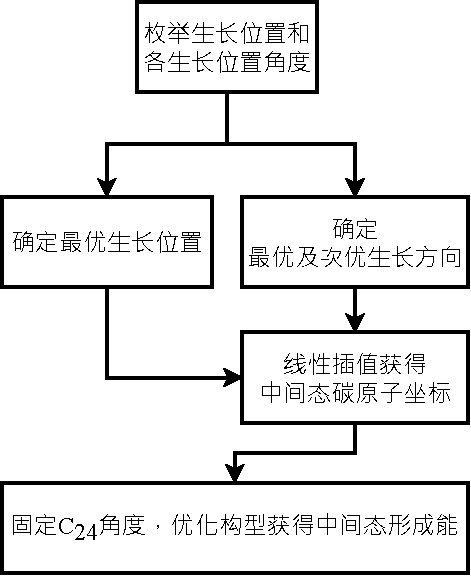
\includegraphics[width=0.4\textwidth]{pic/GO_calculateFlow.pdf}
    }
    \subfloat[]{
        \label{fig:GO_relativeAngle}
        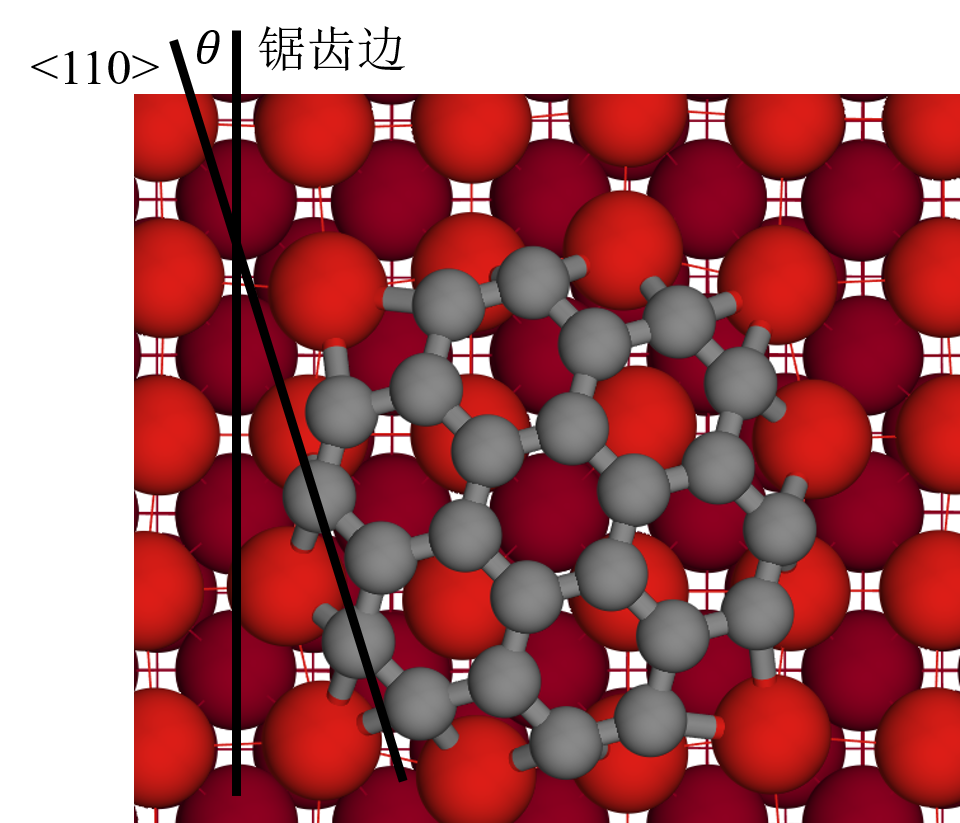
\includegraphics[width=0.4\textwidth]{pic/GO_relativeAngle.png}
    }
    \caption{计算流程图以及$\CCluster{24}$团簇生长角度标识示意图。(a)计算流程图;(b)$\CCluster{24}$团簇在\cemb{Cu}衬底上的生长相对角度标识,其中,\cemb{C}原子为灰色,\cemb{Cu}原子为红色,不同层的\cemb{Cu}原子以不同亮度进行区分}
    \label{fig:GO_calculateFlow_relativeAngle}
\end{figure}

\subsection{石墨烯在平坦\cemb{Cu}衬底表面的生长晶向}
首先对石墨烯$\CCluster{24}$团簇在平坦的\cemb{Cu}衬底表面的优先生长晶向进行探究。如图\ref{fig:GO_001_15_structure}所示,通过计算可以发现在\cemb{Cu(001)}晶面的衬底表面当$\CCluster{24}$团簇中央的空洞位于\cemb{Cu}衬底表面的面心立方位(图\ref{fig:GO_001_15_structure_top}),同时生长角度位$\SI{15}{\degree}$时,所获得的形成能最低。同时,计算获得的$\CCluster{24}$团簇在\cemb{Cu(001)}表面的次优生长方向为$\SI{0}{\degree}$,与先前的文献符合\citing{RN692-2015}。从原子结构上看,石墨烯$\CCluster{24}$团簇边缘的\cemb{C}原子与衬底表面的\cemb{Cu}原子具有较强的相互作用。边缘\cemb{C}原子与衬底表面\cemb{Cu}原子的成键使得$\CCluster{24}$团簇的中央拱起,同时也使得$\CCluster{24}$团簇向更多边缘成键的角度旋转,由此在\cemb{Cu(001)}表面形成了$\SI{15}{\degree}$的优先生长方向。

\begin{figure}[htb]
    \subfloat[]{
        \label{fig:GO_001_15_structure_side}
        \begin{overpic}[width=0.4\textwidth]{pic/GO_C24_flat_001_15deg_structure_side.png}
            \put(85,75){$(0 0 1)$}
        \end{overpic}
    }
    \subfloat[]{
        \label{fig:GO_001_15_structure_top}
        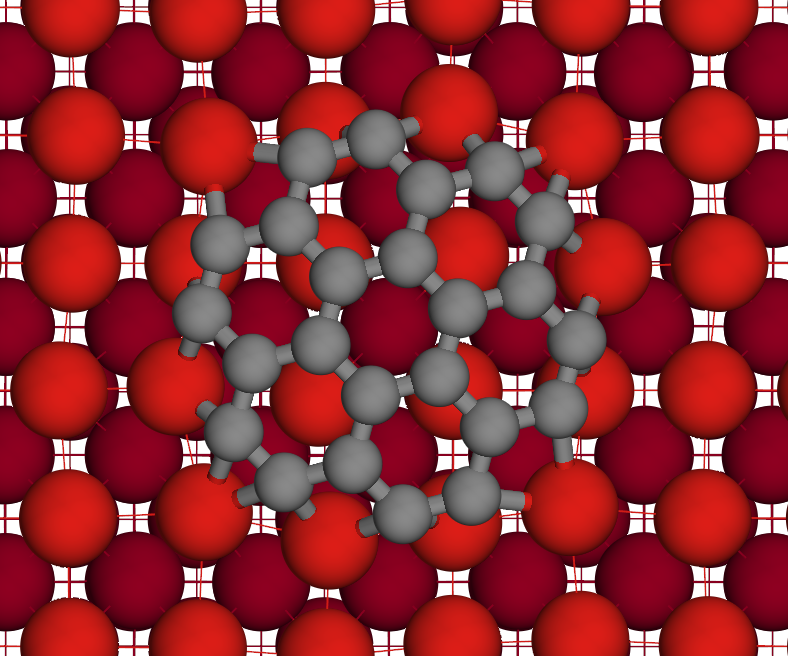
\includegraphics[width=0.4\textwidth]{pic/GO_C24_flat_001_15deg_structure_top.png}
    }

    \caption{\cemb{Cu(001)}晶面石墨烯$\CCluster{24}$团簇的最优生长晶向(\SI{15}{\degree})及原子构型。(a)原子构型侧视图;(b)原子构型俯视图。图中,\cemb{C}原子为灰色,\cemb{Cu}原子为红色,不同层的\cemb{Cu}原子以不同亮度进行区分}
    \label{fig:GO_001_15_structure}
\end{figure}

图\ref{fig:GO_001_energy}给出了通过插值法计算得出的$\CCluster{24}$团簇在\cemb{Cu(001)}表面各个角度的相对形成能。$\CCluster{24}$团簇在平坦的\cemb{Cu(001)}表面具有两个不重合的能量最小值,分别位于$\SI{+15}{\degree}$和$\SI{-15}{\degree}$。$\CCluster{24}$团簇在$\SI{0}{\degree}$和$\SI{30}{\degree}$的生长方向处于能量最高值。从能量最高的生长角度到能量最低的生长角度,$\CCluster{24}$团簇在中间态的相对能量逐渐下降。由于$\CCluster{24}$团簇在旋转至最低能态的过程中均为放热反应,因此绝大部分在成核阶段未处于最优生长方向的石墨烯晶畴会在热力学的作用下逐渐向$\SI{\pm 15}{\degree}$ 的生长晶向靠拢。在\cemb{Cu(001)}表面,$\SI{\pm 15}{\degree}$ 的石墨烯$\CCluster{24}$团簇互为镜面对称,具有相同的形成能。因此在成核生长的过程中,约有一半的石墨烯畴会采取$\SI{-15}{\degree}$的晶向生长,而另一半则会生长为$\SI{+15}{\degree}$的石墨烯畴。从原子结构的角度来看,互为镜像的$\SI{\pm 15}{\degree}$生长的石墨烯畴在几何上并不重叠,由此导致了许多实验中观察到的石墨烯晶畴的非定向生长\citing{RN1062-2012}。

\begin{figure}[htb]
    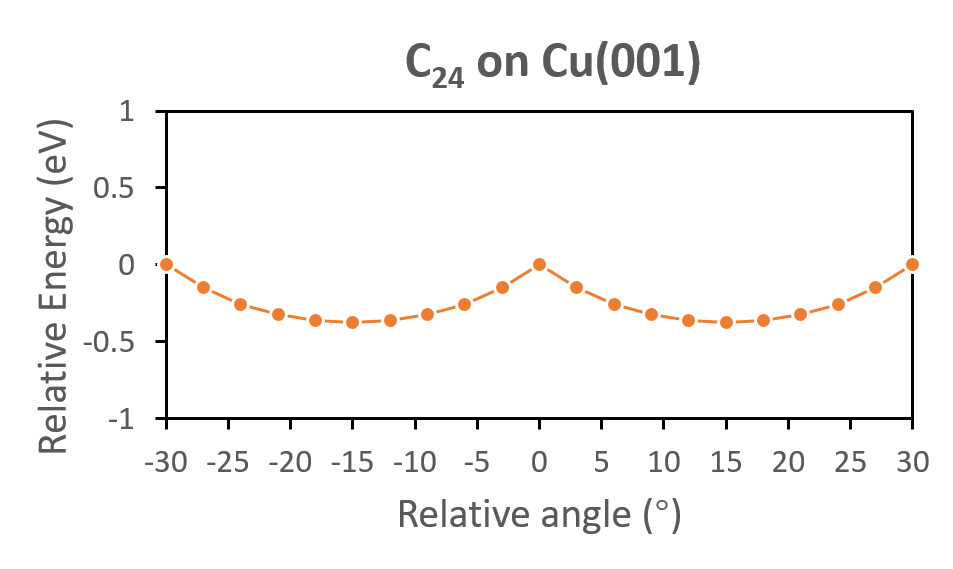
\includegraphics[width=0.8\textwidth]{pic/GO_C24_flat_001_energy.png}
    \caption{\cemb{Cu(001)}晶面上不同生长角度的石墨烯$\CCluster{24}$团簇的相对形成能分布。各生长角度相对形成能的参考构型为生长角度$\SI{0}{\degree}$的构型}
    \label{fig:GO_001_energy}
\end{figure}

另一个常用于生长石墨烯的\cemb{Cu}衬底晶面为\cemb{Cu(111)}面。在平坦的\cemb{Cu(111)}面,可以运用在平坦的\cemb{Cu(001)}表面类似的方法对$\CCluster{24}$团簇的最优生长位点和最优生长方向进行计算。如图\ref{fig:GO_111_structure}所示,不同于在\cemb{Cu(001)}表面$\CCluster{24}$团簇在平坦的\cemb{Cu(111)}表面上的最优生长位点为团簇中央空位垂直于\cemb{Cu(111)}表面原子的顶端(图\ref{fig:GO_111_structure_top})。经过优化后的$\CCluster{24}$团簇的最优生长角度为$\SI{\pm 18}{\degree}$。$\CCluster{24}$团簇边缘的\cemb{C}原子同样也和\cemb{Cu(111)}衬底表面的\cemb{Cu}原子形成了较强的键合,使$\CCluster{24}$团簇呈现处拱起的几何形貌。$\CCluster{24}$团簇在\cemb{Cu(111)}表面和\cemb{Cu(001)}表面优先生长位点和方向的不同可能是来源于不同晶面指数表面对称性的变化。对于单层的\cemb{Cu(001)}表面,其空间对称群为$P4/mmm$,为四方对称。对于单层的\cemb{Cu(111)}表面,其空间对称群为$P6/mmm$,为六方对称。

\begin{figure}[htb]
    \subfloat[]{
        \label{fig:GO_111_structure_side}
        \begin{overpic}[width=0.4\textwidth]{pic/GO_C24_flat_111_18deg_structure_side.png}
            \put(80,75){(111)}
        \end{overpic}
    }
    \subfloat[]{
        \label{fig:GO_111_structure_top}
        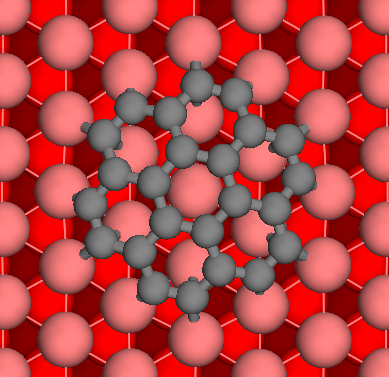
\includegraphics[width=0.4\textwidth]{pic/GO_C24_flat_111_18deg_structure_top.png}
    }

    \caption{\cemb{Cu(111)}晶面石墨烯$\CCluster{24}$团簇的最优生长晶向($\SI{18}{\degree}$)及原子构型。(a)原子构型侧视图;(b)原子构型俯视图。图中,\cemb{C}原子为灰色,\cemb{Cu}原子为红色,不同层的\cemb{Cu}原子以不同亮度进行区分}

    \label{fig:GO_111_structure}
\end{figure}

图\ref{fig:GO_111_energy}给出了利用插值法得出的在平坦的\cemb{Cu(111)}表面石墨烯$\CCluster{24}$团簇在最优生长角度之间的中间态进行形成能分布情况。$\CCluster{24}$团簇在\cemb{Cu(111)}上的次优生长方向为$\SI{\pm 30}{\degree}$。由于衬底对称性的变化,在\cemb{Cu(111)}表面,$\SI{0}{\degree}$ 方向生长的$\CCluster{24}$团簇与$\SI{\pm 30}{\degree}$方向生长的$\CCluster{24}$团簇并不等价。具体而言,遵循$\SI{0}{\degree}$ 方向生长的$\CCluster{24}$团簇的锯齿(zigzag)边与\cemb{Cu(111)}衬底的$\langle 110\rangle$方向平行,扶手椅(armchair)边与$\langle\bar{1}\bar{1}2\rangle$方向平行。而遵循$\SI{\pm 30}{\degree}$方向生长的$\CCluster{24}$团簇则相反,扶手椅(armchair)边与\cemb{Cu(111)}衬底的$\langle 110\rangle$方向平行,锯齿(zigzag)边与$\langle\bar{1}\bar{1}2\rangle$方向平行。\cemb{Cu}$\langle\bar{1}\bar{1}2\rangle$晶向的原子间距为$\SI{4.23}{\angstrom}$,高于\cemb{Cu}$\langle 110\rangle$晶向中$\SI{2.56}{\angstrom}$的\cemb{Cu}原子间距。从计算结果上看,$\SI{\pm 30}{\degree}$方向生长的$\CCluster{24}$团簇的形成能比$\SI{0}{\degree}$ 方向生长的$\CCluster{24}$团簇低大约$\SI{0.9}{\electronvolt}$。与在平坦的\cemb{Cu(001)}晶面上类似,$\CCluster{24}$团簇从任意生长角度到能量最低的$\SI{\pm 18 }{\degree}$的中间态的能量逐渐下降。$\CCluster{24}$团簇在转向最优生长角度的过程均为放热反应,因此绝大部分在成核阶段未处于最优生长方向的石墨烯晶畴会在热力学的作用下逐渐向$\SI{\pm 18}{\degree}$ 的生长晶向靠拢。从原子结构的角度来看,互为镜像的$\SI{\pm 18}{\degree}$ 石墨烯畴在几何上并不重叠。在生长过程中的不同晶畴进行融合时仍会产生晶界。

\begin{figure}[htb]
    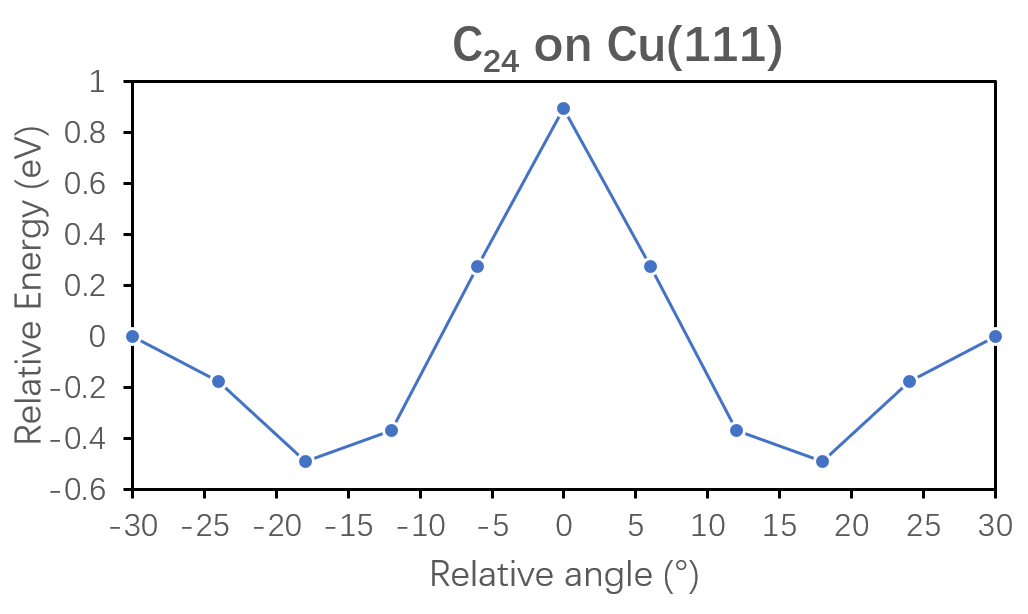
\includegraphics[width=0.8\textwidth]{pic/GO_C24_flat_111_energy.png}
    \caption{\cemb{Cu(111)}晶面上不同生长角度的石墨烯$\CCluster{24}$团簇的相对形成能分布。各生长角度相对形成能的参考构型为生长角度$\SI{\pm 30}{\degree}$的构型}
    \label{fig:GO_111_energy}
\end{figure}

\subsection{石墨烯在\cemb{Cu}表面台阶处的生长晶向}
本小节主要关注石墨烯$\CCluster{24}$团簇在晶面指数为(11n) ($\rm{n \geqslant 1}$)的\cemb{Cu}衬底的优先生长晶向。晶面指数为(11n) ($\rm{n \geqslant 1}$)的\cemb{Cu}表面结构可以看成由不同密度的\cemb{Cu(001)}台面或者\cemb{Cu(111)}台面组合而成。因此,可以将晶面指数为(11n) ($\rm{n \geqslant 1}$)的\cemb{Cu}衬底分为两类\chinesecolon 一类可以看作以\cemb{Cu(001)}台面组合而成,台阶的方向为\cemb{Cu}$\langle 110\rangle$晶向,这类同衬底的晶面指数为(11n) ($\rm{n \geqslant 3}$)。另一类可以看作以\cemb{Cu(111)}台面组合,台阶方向同样为\cemb{Cu}$\langle 110\rangle$晶向,这类\cemb{Cu}衬底的晶面指数为(11n) ($\rm{1 \leqslant n \leqslant 3}$)。而作为二者之间的\cemb{Cu(113)}晶面,是两原子宽的\cemb{Cu(001)}晶面加上两原宽的\cemb{Cu(111)}晶面相对搭接而成。因此,在\cemb{Cu(113)}表面的台阶,既可以看成是(001)台面,也可以看成是(111)台面。

\begin{table}[htb]
    \centering
    \caption{石墨烯$\CCluster{24}$团簇在平坦\cemb{Cu(001)}衬底以及$\langle 110\rangle$台阶边缘的形成能}
    \begin{tabular}{cc}
        \toprule
        衬底类型                                         & 形成能(\si{\electronvolt})  \\
        \midrule
        平坦\cemb{Cu(001)}衬底                           & $-6.24$                      \\
        \cemb{Cu(001)}衬底的$\langle 110\rangle$台阶边缘  & $-9.02$                      \\
        \bottomrule
    \end{tabular}
    \label{tab:GO_flat_vs_step}
\end{table}

上一节的计算表明石墨烯$\CCluster{24}$团簇边缘的\cemb{C}原子与衬底表面\cemb{Cu}原子之间产生了较强的相互作用,从而导致了不同晶面的\cemb{Cu}衬底表面$\CCluster{24}$团簇不同的的优先生长角度。而进一步计算发现,$\CCluster{24}$团簇边缘\cemb{C}原子在\cemb{Cu}衬底表面的台阶处有相比于平坦衬底更强烈的相互作用(表\ref{tab:GO_flat_vs_step})。为了使台阶边缘生长的$\CCluster{24}$团簇的形成能与在平坦台面生长的$\CCluster{24}$团簇的形成能具有可比性。在台阶边缘生长的$\CCluster{24}$团簇的形成能同样使用式\eqref{eq:GO_formationE}进行计算。计算结果显示,倘若\cemb{Cu(001)}衬底表面有一个晶向为$\langle 110\rangle$的台阶,$\CCluster{24}$团簇在台阶边缘的形成能为$E_{\rm f}^{\rm step}=\SI{-9.02}{\electronvolt}$,大大低于在平坦\cemb{Cu(001)}衬底表面的形成能$E_{\rm f}^{\rm flat}=\SI{-6.24}{\electronvolt}$。因此可以判断,石墨烯更倾向于在\cemb{Cu}衬底的台阶处成核。

对于以\cemb{Cu(001)}为台面的\cemb{Cu(11n)} ($\rm{n \geqslant 3}$)衬底。由于石墨烯团簇与\cemb{Cu}衬底的相互作用主要集中在团簇边缘的未饱和\cemb{C}原子。并且台阶作为台面的边缘会极大的影响石墨烯团簇与\cemb{Cu}衬底的形成能。为了不失一般性,本小节的研究中以$\CCluster{24}$团簇的直径作为参考,建立了三个代表性的\cemb{Cu}衬底模型。这三个模型分别对应于台面长度小于$\CCluster{24}$团簇直径的\cemb{Cu(115)}晶面;台面长度大致等于$\CCluster{24}$团簇直径的\cemb{Cu(117)}晶面;以及台面长度远大于小于$\CCluster{24}$团簇直径的(11X) ($\rm X \gg 7 $)晶面。

%figure 11X
\begin{figure}[!b]
    \centering
    \subfloat[]{
        \label{fig:GO_11X_structure_side}
        \begin{overpic}[width=0.4\textwidth,trim={40 0 40 0},clip]{pic/GO_11X_structure_side.png}
            \put(85,60){$\rm (1 1 X)$}
        \end{overpic}
    }
    \subfloat[]{
        \label{fig:GO_11X_structure_top}
        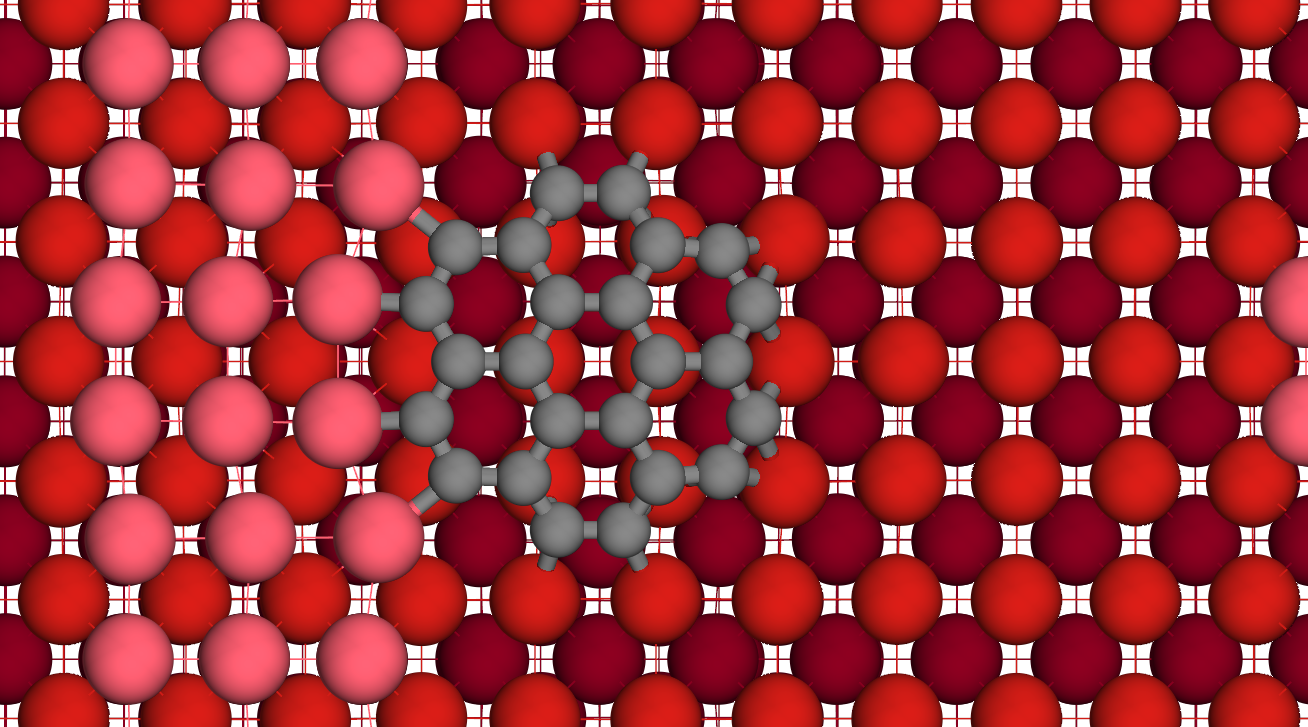
\includegraphics[width=0.4\textwidth,trim={60 20 150 20},clip]{pic/GO_11X_structure_top.png}
    }
\end{figure}
\begin{figure}\ContinuedFloat
    \subfloat[]{
        \label{fig:GO_11X_structure_energy}
        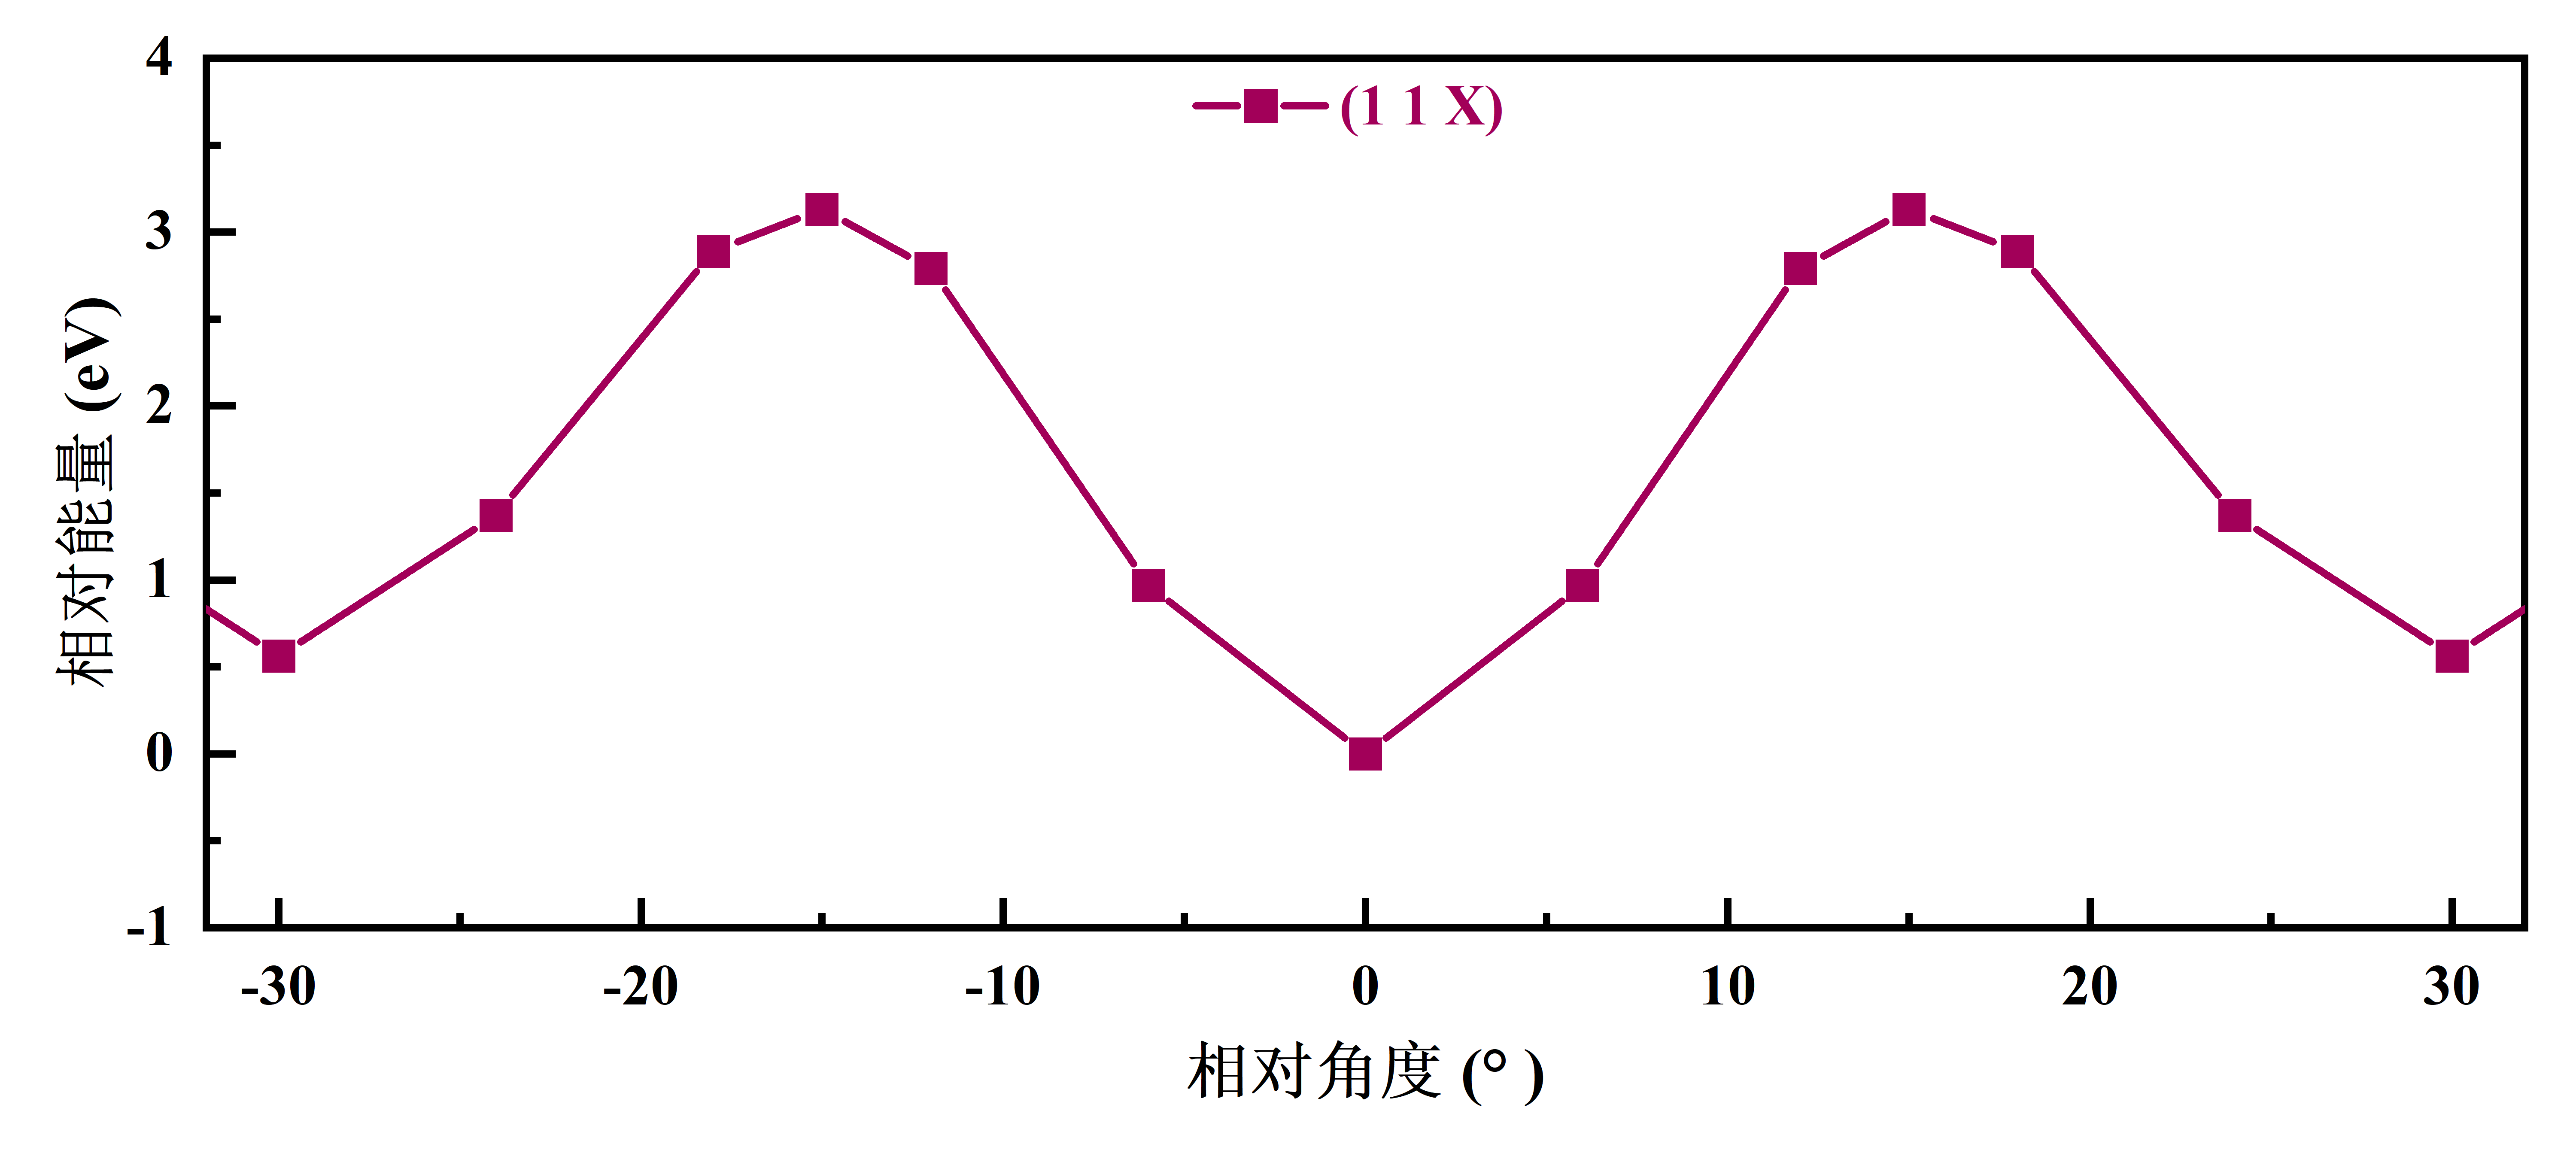
\includegraphics[width=0.8\textwidth]{pic/GO_C24_11X_energy.png}
    }
    \caption{\cemb{Cu(11X)}晶面上石墨烯$\CCluster{24}$团簇的最优生长晶向(\SI{0}{\degree})、原子构型以及各生长角度能量分布图。(a)原子构型侧视图;(b)原子构型俯视图;(c)各生长角度能量分布。图中,\cemb{C}原子为灰色,\cemb{Cu}原子为红色,不同层的\cemb{Cu}原子以不同亮度进行区分}
    \label{fig:GO_C24_11X}
\end{figure}

对于台面长度远大于小于$\CCluster{24}$团簇直径的(11X) ($\rm X \gg 7 $)晶面(图\ref{fig:GO_C24_11X}),计算结果显示当$\CCluster{24}$团簇在台阶处成核生长时$\CCluster{24}$团簇的最优成核位置位于台阶的下方(图\ref{fig:GO_11X_structure_side}和图\ref{fig:GO_11X_structure_top}),$\CCluster{24}$团簇的中央空洞位于\cemb{Cu(001)}台面的六方密堆位。此时一半的$\CCluster{24}$团簇边缘与\cemb{Cu}$\langle 110\rangle$台阶成键,另一半与\cemb{Cu(001)}台面成键。相对于在平坦的\cemb{Cu(001)}表面,$\CCluster{24}$团簇在\cemb{Cu(11X)}表面的两个不重叠的最优生长角度,由于台阶的作用产生了劈裂和偏移,出现了最优生长角度和次优生长角度。

从图\ref{fig:GO_11X_structure_energy}中可以看到,$\CCluster{24}$团簇在\cemb{Cu(11X)}表面的台阶处的最优生长角度为$\SI{0}{\degree}$,次优生长角度为$\SI{\pm 30 }{\degree}$。最优和次优生长角度之间的能量差为$\SI{0.56 }{\electronvolt}$。$\SI{\pm 30 }{\degree}$和$\SI{0}{\degree}$的生长角度之间,有约为$\SI{2.56}{\electronvolt}$的旋转势垒。单一的最优生长角度使得$\CCluster{24}$团簇在\cemb{Cu(11X)}衬底的台阶处展现出定向生长的趋势。较高的旋转势垒使得$\CCluster{24}$团簇在成核生长的过程中需要需要较高的温度才能从次优的$\SI{\pm 30 }{\degree}$生长角度旋转至最优的$\SI{0 }{\degree}$。同时,由于\cemb{Cu(11X)}衬底的(001)台面具有高于$\CCluster{24}$团簇直径的宽度,因此石墨烯晶畴很可能在远离$\langle 110\rangle$台阶的位置成核生长。在远离$\langle 110\rangle$台阶的位置成核生长的石墨烯晶畴类似于在平坦\cemb{Cu(001)}衬底的表面生长。此时生长的石墨烯晶畴则缺乏热力学上的定向趋势。因此在\cemb{Cu(11X)}乃至于\cemb{Cu(001)}表面很难实现石墨烯晶畴的定向生长。

%figure 117 115
\begin{figure}[!htb]
    \subfloat[]{
        \label{fig:GO_117_structure_side}
        \begin{overpic}[width=0.4\textwidth,trim={60 40 40 0},clip]{pic/GO_117_structure_side.png}
            \put(85,53){(117)}
        \end{overpic}
    }
    \subfloat[]{
        \label{fig:GO_117_structure_top}
        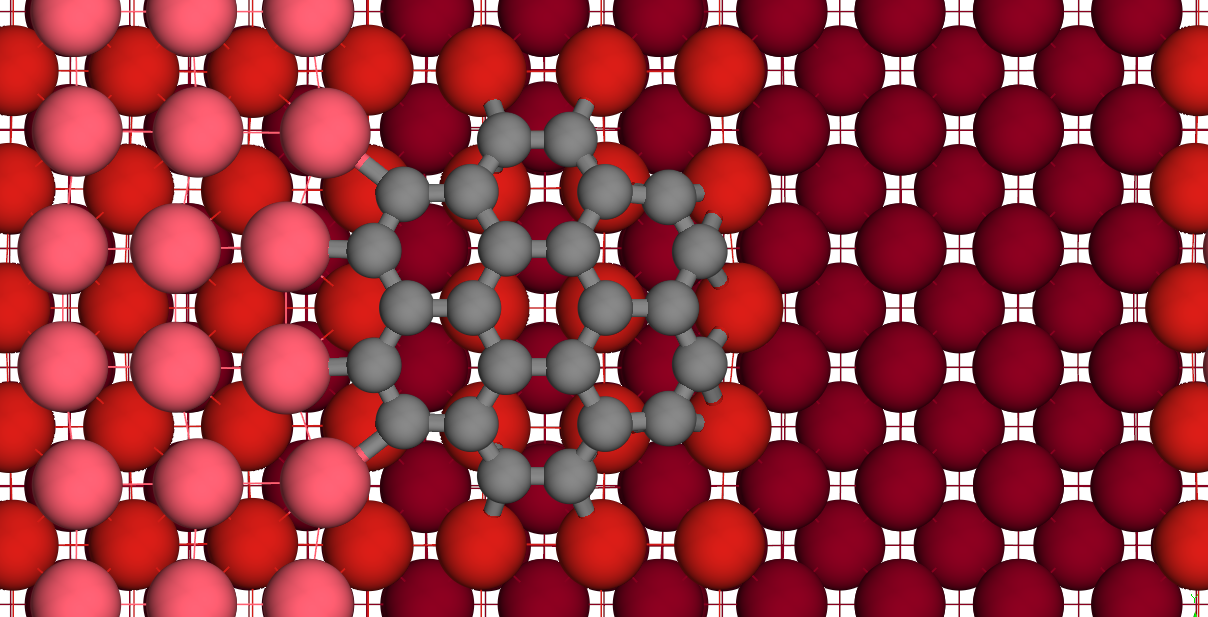
\includegraphics[width=0.4\textwidth,trim={40 0 60 0},clip]{pic/GO_117_structure_top.png}
    }\\[-1ex]
    \subfloat[]{
        \label{fig:GO_115_structure_side}
        \begin{overpic}[width=0.4\textwidth,trim={60 80 40 10},clip]{pic/GO_115_structure_side.png}
            \put(85,53){(115)}
        \end{overpic}
    }
    \subfloat[]{
        \label{fig:GO_115_structure_top}
        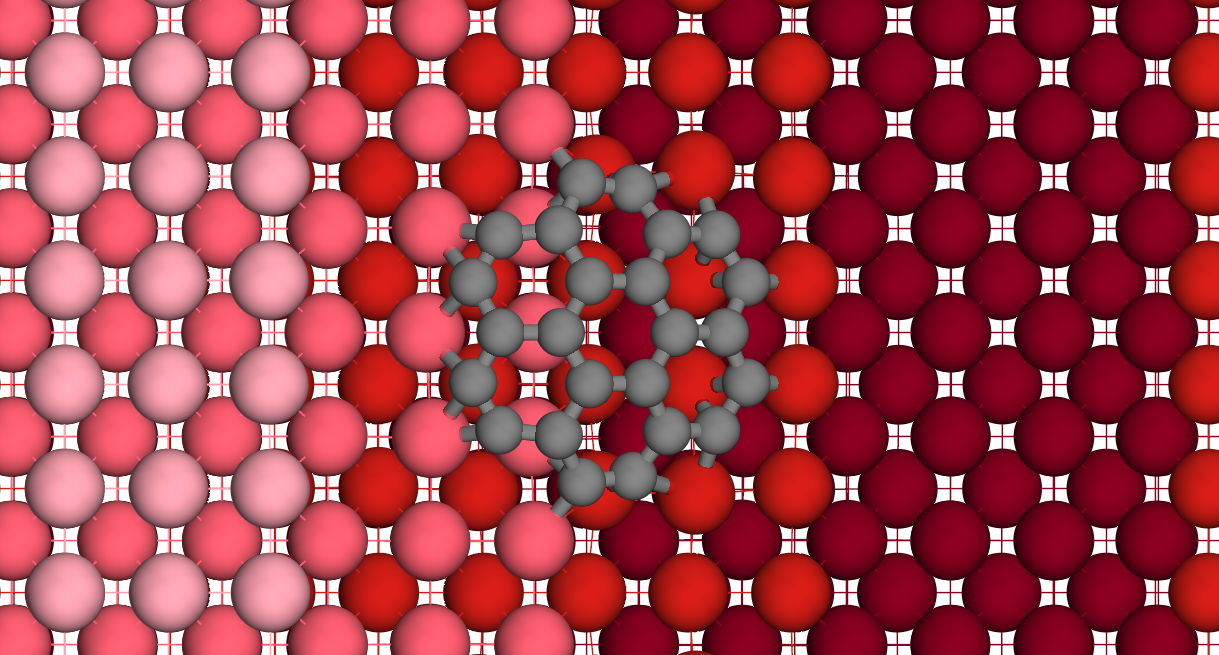
\includegraphics[width=0.4\textwidth,trim={60 20 120 40},clip]{pic/GO_115_structure_top.png}
    }\\[-0.5ex]
    \subfloat[]{
        \label{fig:GO_C24_117_115_energy}
        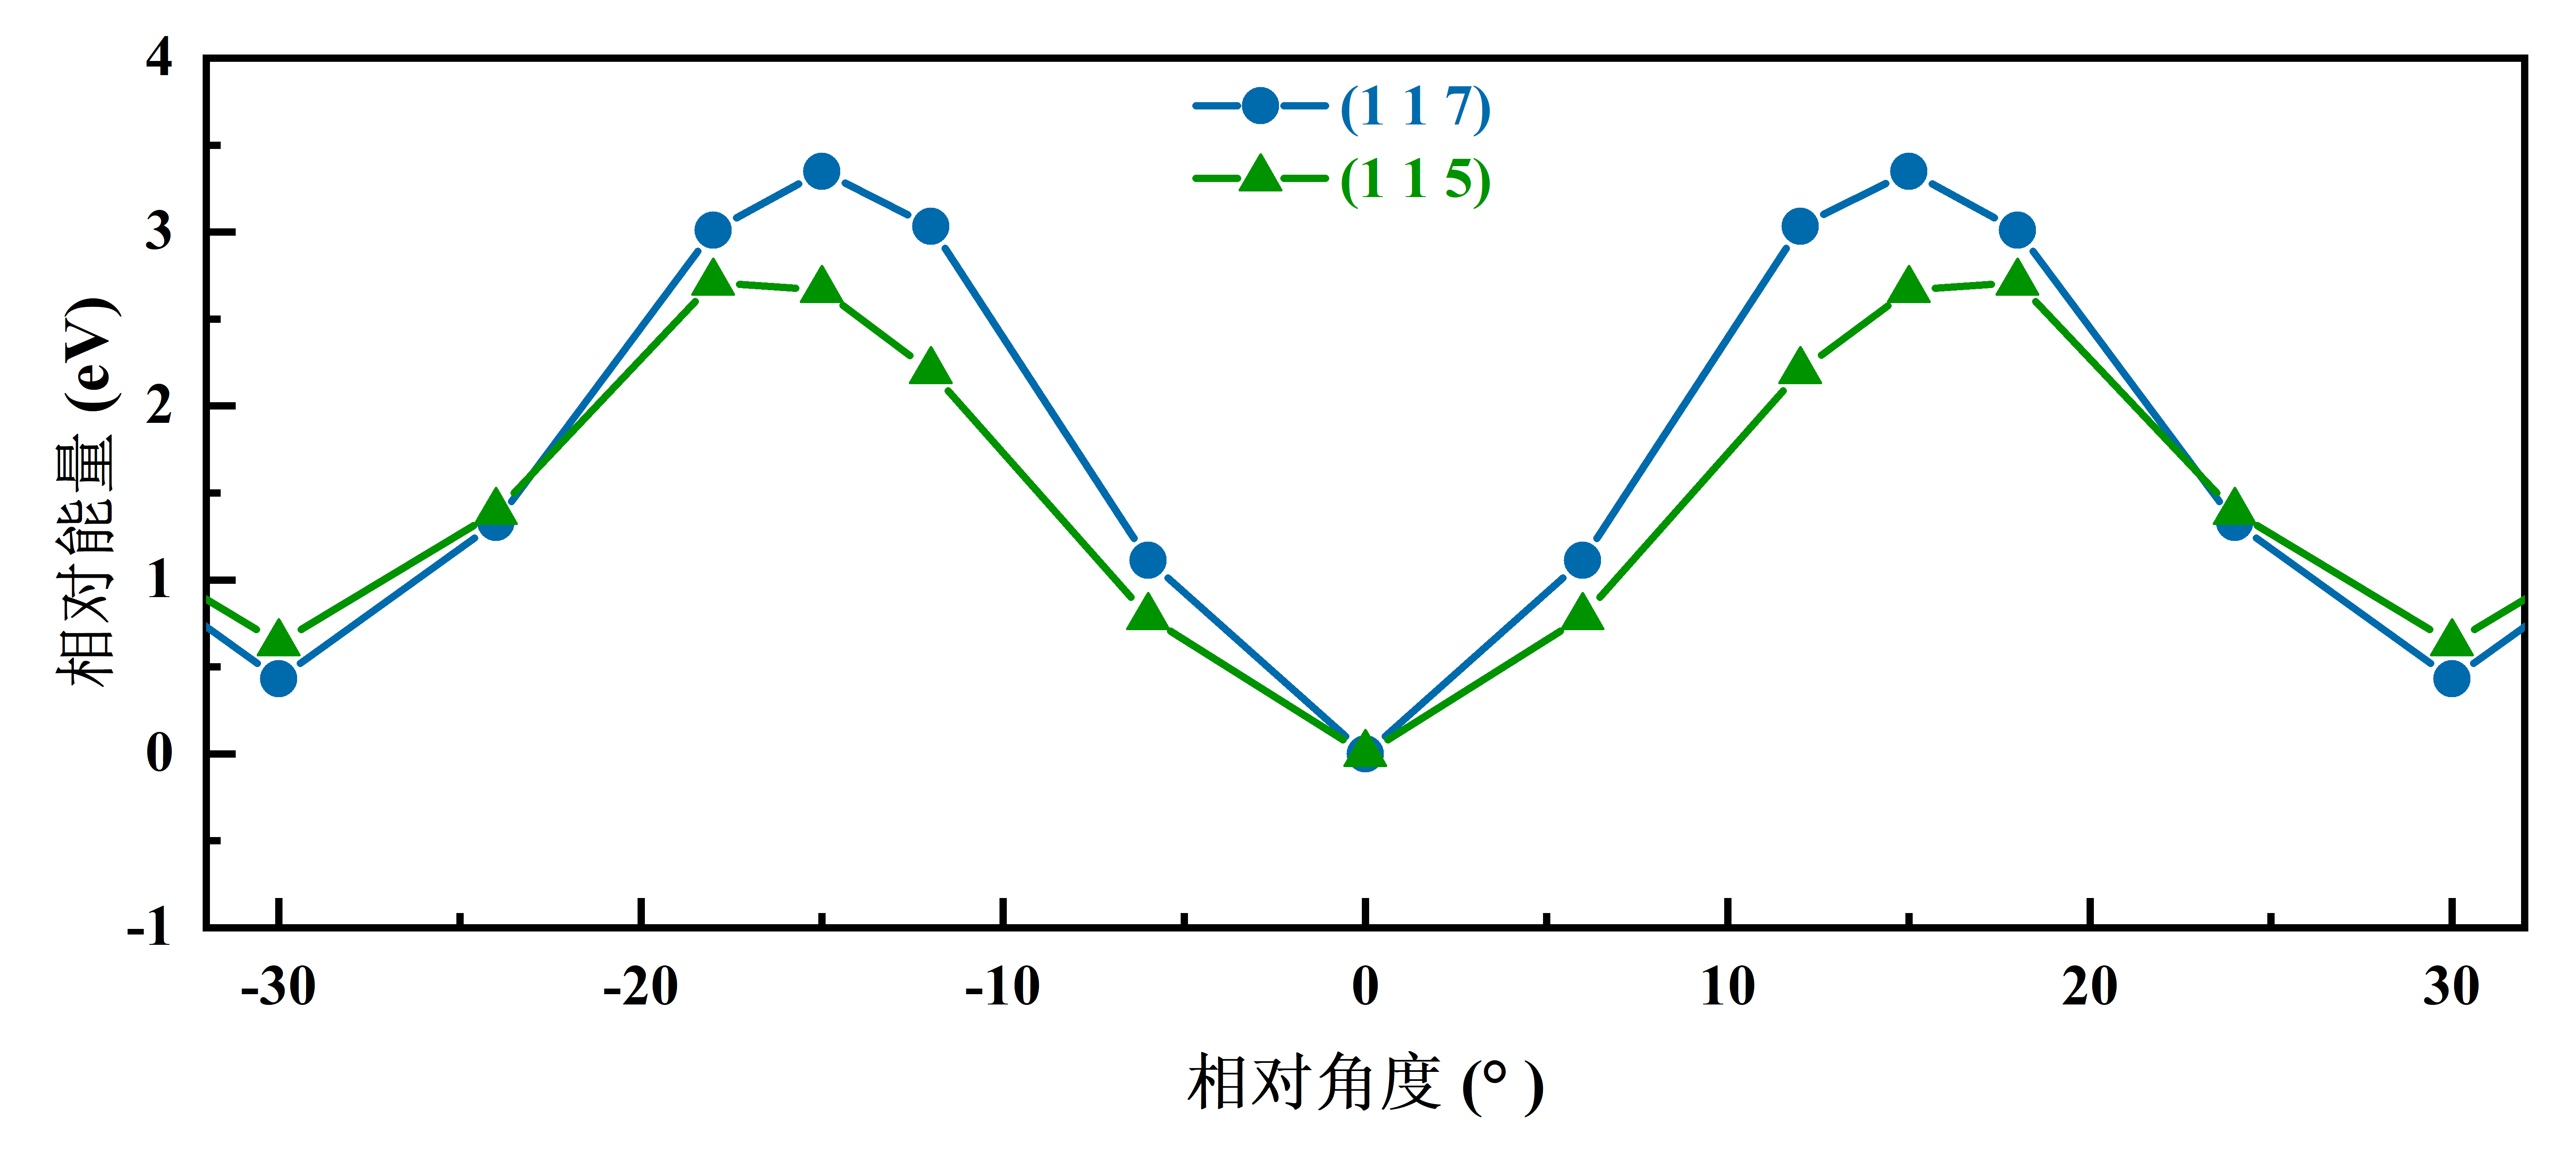
\includegraphics[width=0.8\textwidth]{pic/GO_C24_117_115_energy.png}
    }
    \caption{\cemb{Cu(117)}与(115)晶面上石墨烯$\CCluster{24}$团簇的最优生长晶向(\SI{0}{\degree})、原子构型以及各生长角度能量分布图。(a) (117)晶面原子构型侧视图;(b) (117)晶面俯视图;(c) (115)晶面最优生长角度原子构型侧视图;(d) (115)晶面俯视图;(e) (117)与(115)晶面上$\CCluster{24}$团簇各生长角度能量分布。图中,\cemb{C}原子为灰色,\cemb{Cu}原子为红色,不同层的\cemb{Cu}原子以不同亮度进行区分}
    \label{fig:GO_C24_117_115}
\end{figure}

$\CCluster{24}$团簇在\cemb{Cu(117)}以及(115)晶面的台阶处的生长情况与\cemb{Cu(11X)}表面相似(图\ref{fig:GO_C24_117_115})。在\cemb{Cu(117)}晶面上,由于(001)台面的宽度与$\CCluster{24}$团簇的直径相近,$\CCluster{24}$团簇的一边与第一层台阶下边缘成键,另一层与第二层台阶的上边缘成键(图\ref{fig:GO_117_structure_side}和图\ref{fig:GO_117_structure_top})。$\CCluster{24}$团簇在\cemb{Cu(117)}表面的最优生长位置同样也为\cemb{Cu(001)}台面的六方密堆位。而对于\cemb{Cu(115)}晶面台阶处的$\CCluster{24}$团簇生长,由于\cemb{Cu(115)}晶面上的\cemb{Cu(001)}台面宽度仅有2原子宽,短于$\CCluster{24}$团簇的直径,所以$\CCluster{24}$团簇无法与第一层台阶的下边缘成键(图\ref{fig:GO_115_structure_side}和图\ref{fig:GO_115_structure_top})。导致在\cemb{Cu(115)}晶面上,$\CCluster{24}$团簇的一边与第二层的台面成键,另一边与第三层台阶的上边缘成键。与第二层台阶具有较强相互作用的则是位于$\CCluster{24}$团簇中部的边缘原子。同时,由于$\CCluster{24}$团簇在(115)晶面上的生长需要横跨两层台阶,其最优生长位点相对于(11X)以及(115)晶面也有所变化。正对$\CCluster{24}$团簇中央空位的衬底位点由在(001)台面上的六方密堆位移动至面心立方位。

从能量的角度上看(图\ref{fig:GO_C24_117_115_energy}),$\CCluster{24}$团簇在\cemb{Cu(117)}以及(115)晶面的上的最优生长角度均为$\SI{0 }{\degree}$,次优生长角度位$\SI{\pm 30 }{\degree}$,与\cemb{Cu(11X)}晶面台阶处一致。在\cemb{Cu(117)}晶面上,$\CCluster{24}$团簇在次优生长角度和最优生长角度之间的能量差为$\SI{0.43}{\electronvolt}$。这个能量差低于$\CCluster{24}$团簇在\cemb{Cu(11X)}晶面台阶边缘的$\SI{0.56}{\electronvolt}$次优-最优角能量差,导致在\cemb{Cu(117)}晶面上$\CCluster{24}$团簇从次优生长角转向最优生长角的比例不及生长在(11X)晶面台阶处的$\CCluster{24}$团簇,使得\cemb{Cu(117)}晶面上生长的石墨烯的定向性下降。同时,$\CCluster{24}$团簇从次优的$\SI{\pm 30 }{\degree}$生长角度转向最优的$\SI{0}{\degree}$需要克服的旋转势垒为$\SI{2.91 }{\electronvolt}$,同样高于$\CCluster{24}$团簇在\cemb{Cu(11X)}晶面台阶处的旋转势垒。较高的旋转势垒会导致$\CCluster{24}$团簇从次优生长角向最优生长角的转变难度上升,需要更多的能量或者更长的时间才能反应至最稳态。由于石墨烯晶畴的成核生长与石墨烯晶畴向最优生长角的转变是同时进行的,石墨烯晶畴的进一步生长会引入更多的边缘原子与衬底键合,可能会导致旋转势垒提高到无法依靠热能逾越的地步。因此较高的旋转势垒也可能会导致石墨烯晶畴的定向性下降。对于\cemb{Cu(115)}晶面,$\CCluster{24}$团簇在次优生长角度和最优生长角度之间的能量差为$\SI{0.64}{\electronvolt}$,高于\cemb{Cu(117)}晶面以及\cemb{Cu(11X)}晶面。同时对于$\CCluster{24}$团簇,在\cemb{Cu(115)}晶面上成核生长时,在热力学的作用下从次优生长角度旋转至最优生长角度所需要跨越的旋转势垒为$\SI{2.07 }{\electronvolt}$,低于在\cemb{Cu(117)}以及(11X)晶面的旋转势垒。

通过以上计算可以发现,虽然台面的宽度有所差距,但是对于晶面指数为(11n) ($\rm{n \geqslant 3}$)\cemb{Cu}衬底而言,衬底表面的台阶对石墨烯晶畴的生长方向均有限制作用。其中以(115)晶面\cemb{Cu}衬底最能够使石墨烯晶畴依照以$\SI{0 }{\degree}$的生长角度进行定向成核生长。

对于以(111)为台面的\cemb{Cu(112)}晶面,$\CCluster{24}$团簇在其台阶处的成核生长行为与在平坦的\cemb{Cu(111)}衬底表面有较大的不同(图\ref{fig:GO_C24_112})。在\cemb{Cu(112)}晶面,由于台面的宽度短于$\CCluster{24}$团簇的直径,$\CCluster{24}$团簇无法直接于第一层台阶的下边缘成键。优化后的最优构型显示$\CCluster{24}$团簇在\cemb{Cu(112)}晶面上成核生长时倾向于跨越一层\cemb{Cu}$\langle 110\rangle$台阶(图\ref{fig:GO_112_structure_side}和图\ref{fig:GO_112_structure_top})。$\CCluster{24}$团簇的一边与第一层的\cemb{Cu}台面成键,另一边与第二层的\cemb{Cu}台阶的上表面成键。在台阶的作用下,$\CCluster{24}$团簇在\cemb{Cu(112)}台面上的最优生长方向为$\SI{0}{\degree}$。

%figure 112
\begin{figure}[htb]
    \subfloat[]{
        \label{fig:GO_112_structure_side}
        \begin{overpic}[width=0.4\textwidth,trim=30 20 20 0,clip]{pic/GO_112_structure_side.png}
            \put(85,53){$\rm (1 1 2)$}
        \end{overpic}
    }
    \subfloat[]{
        \label{fig:GO_112_structure_top}
        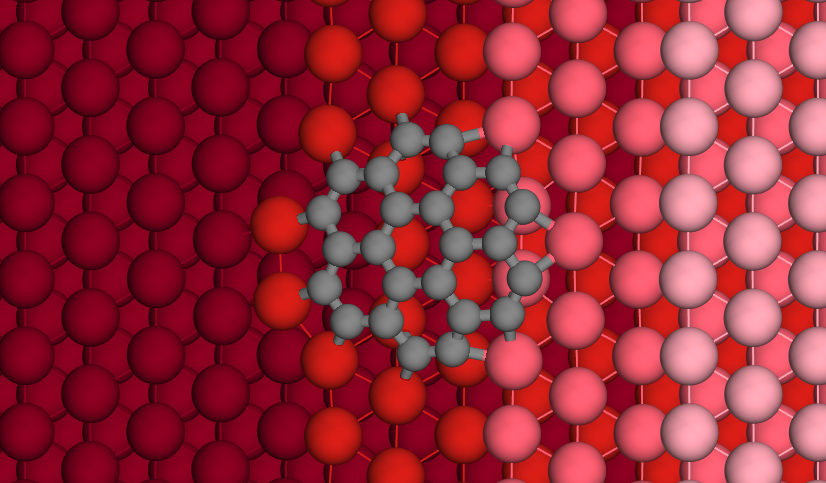
\includegraphics[width=0.4\textwidth,trim=80 40 50 40,clip]{pic/GO_112_structure_top.png}
    }
    \\
%\end{figure}
%\begin{figure}[]\ContinuedFloat
    \subfloat[]{
        \label{fig:GO_112_structure_energy}
        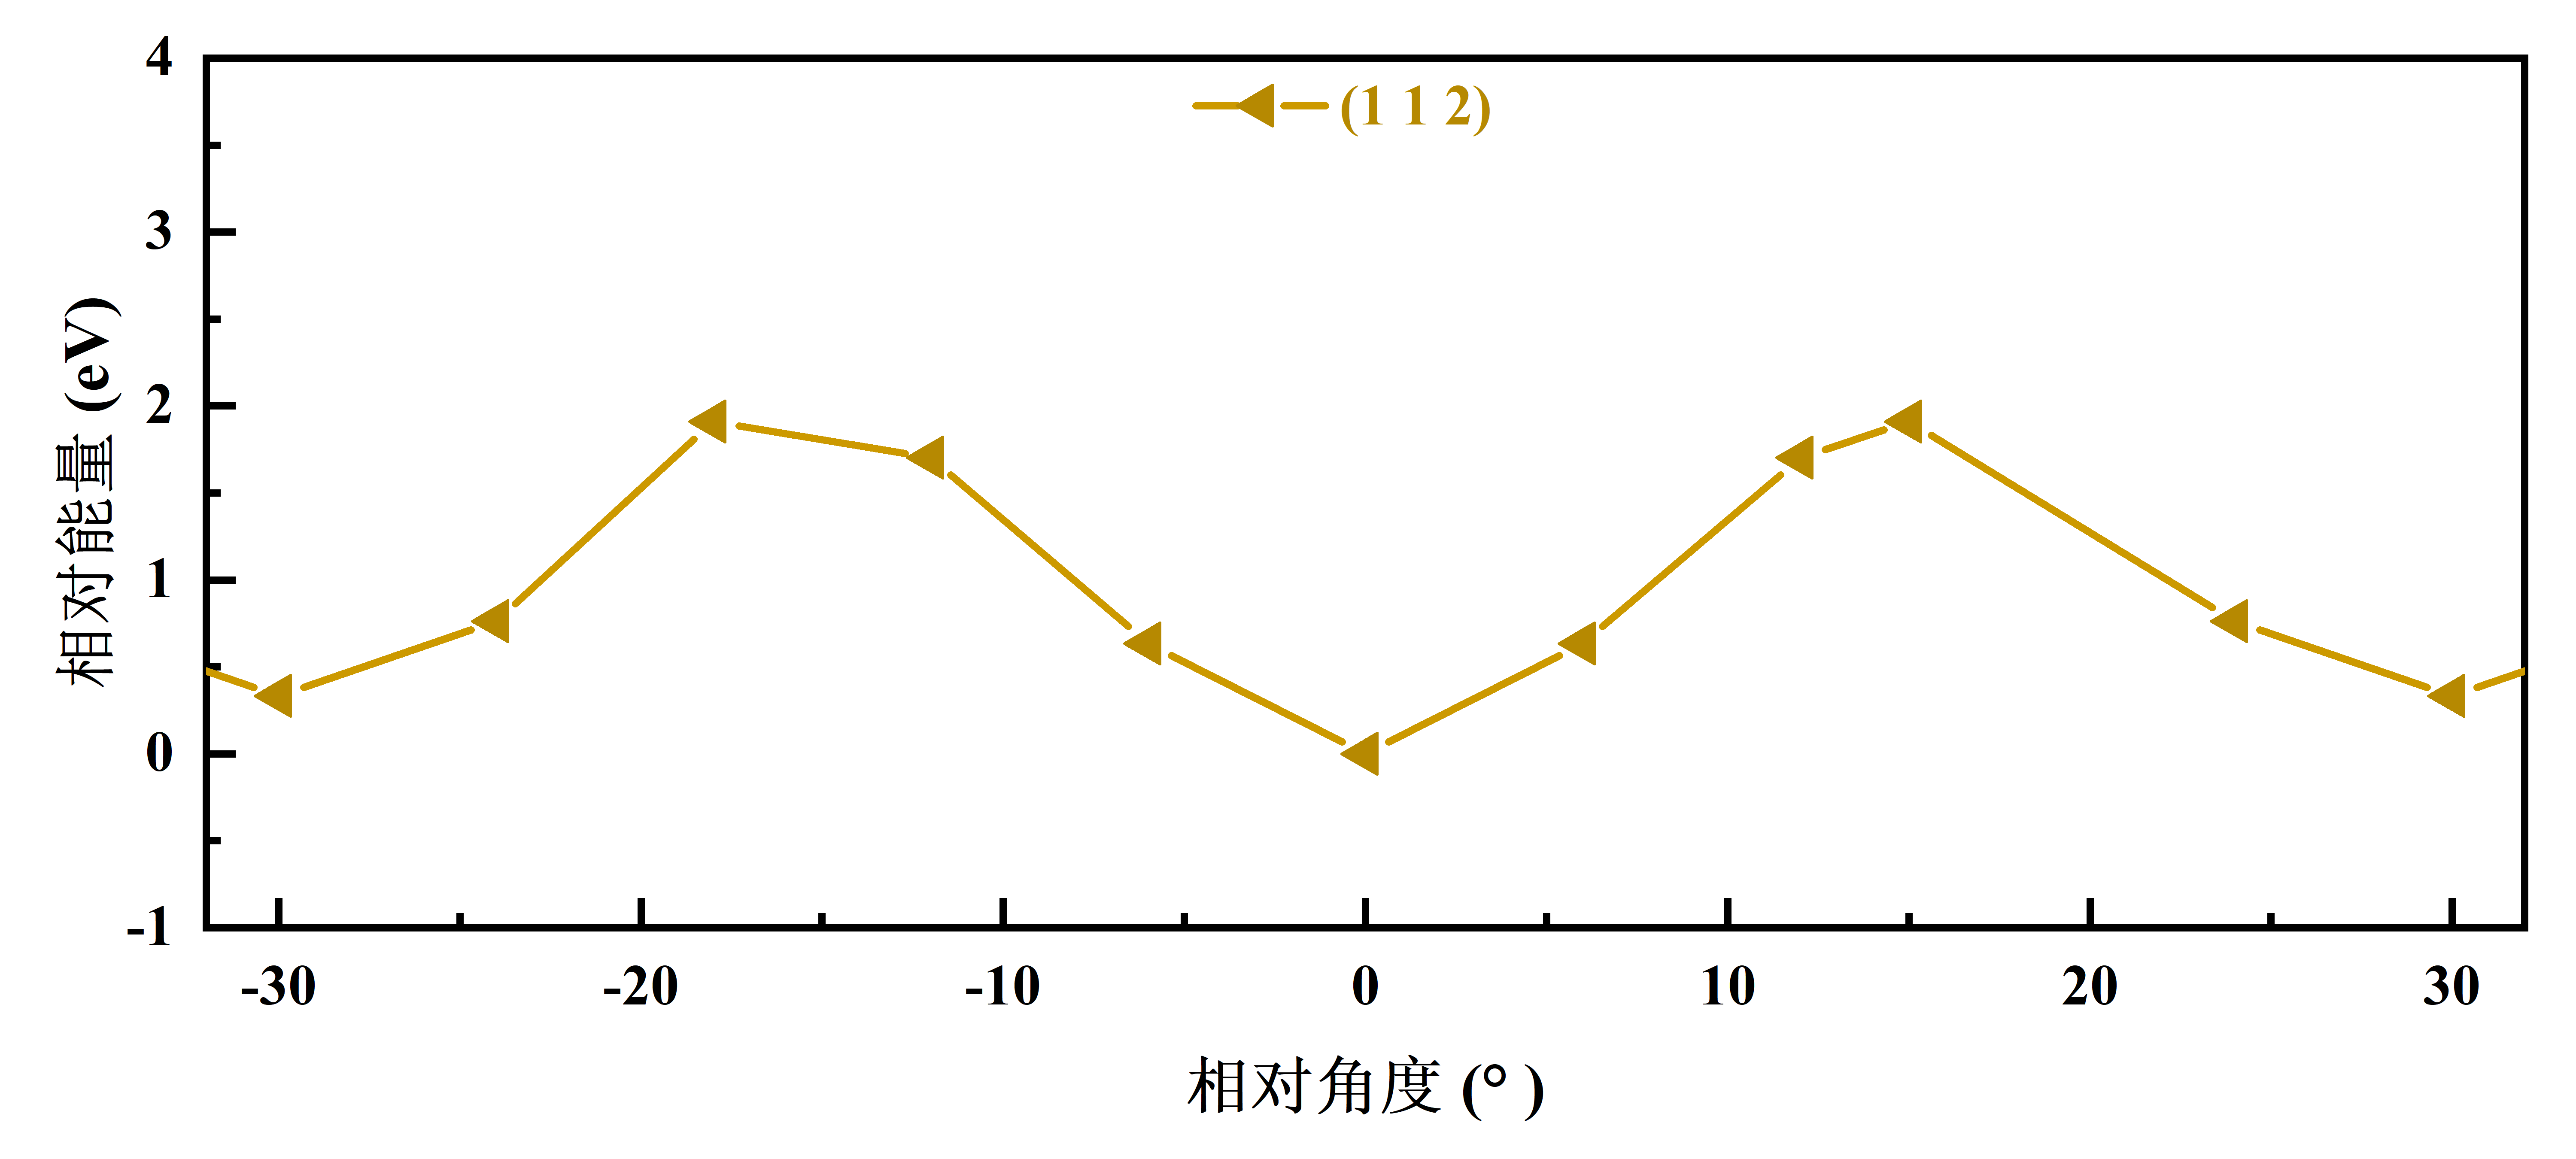
\includegraphics[width=0.8\textwidth]{pic/GO_C24_112_energy.png}
    }
    \caption{\cemb{Cu(112)}晶面上石墨烯$\CCluster{24}$团簇的最优生长晶向(\SI{0}  {\degree})、原子构型以及各生长角度能量分布图。(a)最优生长角度原子构型侧视图;(b)最优生长角度原子构型俯视图;(c)各生长角度能量分布。图中,\cemb{C}原子为灰色,\cemb{Cu}原子为红色,不同层的\cemb{Cu}原子以不同亮度进行区分}
    \label{fig:GO_C24_112}
\end{figure}

如图\ref{fig:GO_112_structure_energy}所示,台阶对于$\CCluster{24}$晶畴边缘\cemb{C}原子较强的相互作用同样使得(111)台面上两个不重叠的最优生长角度($\SI{\pm 18 }{\degree}$)劈裂、偏移至$\SI{0}{\degree}$和$\SI{\pm 30 }{\degree}$。对于\cemb{Cu(112)}晶面,$\CCluster{24}$团簇的最优生长角度为$\SI{0}{\degree}$,次优生长角度为$\SI{\pm 30 }{\degree}$。次优-最优生长角度之间的能量差为$\SI{0.33}{\electronvolt}$,低于先前计算的以\cemb{Cu(001)}台面为基础的台阶模型。可以判断$\CCluster{24}$团簇在\cemb{Cu(112)}衬底上的定向性弱于\cemb{Cu(11n)} ($\rm{n \geqslant 3}$)衬底。旋转势垒方面,在\cemb{Cu(112)}衬底上生长的石墨烯从次优的$\SI{\pm 30 }{\degree}$旋转至最优的$\SI{0}{\degree}$所需要克服的势垒为$\SI{1.57 }{\electronvolt}$,低于\cemb{Cu(11n)} ($\rm{n \geqslant 3}$)衬底衬底。因此在\cemb{Cu(112)}台面,石墨烯晶畴可以在更低的生长温度下从非定向生长演化为定向生长。

而对于\cemb{Cu(113)}面,(001)台面和(111)台面的相互交错不仅使得\cemb{Cu(113)}面具有在晶面指数为(11n) ($\rm{n \geqslant 1}$)这一系列的\cemb{Cu}衬底中拥有最高的表面能\citing{RN1063-1993},同时也对石墨烯$\CCluster{24}$团簇的定向产生了极大的影响。从图\ref{GO_C24_113}中可以看到,在\cemb{Cu(113)}面上$\CCluster{24}$团簇的最优生长构型不仅横跨两个\cemb{Cu}台面,同时团簇两边的边缘\cemb{C}原子都与$\langle 110\rangle$台阶产生了强烈的相互作用。同时,$\CCluster{24}$团簇在\cemb{Cu(113)}表面的最优生长角度也发生了变化,为几何相互不重叠的$\SI{\pm 27 }{\degree}$。因此,类似平坦的\cemb{Cu(001)}表面以及\cemb{Cu(111)}表面,石墨烯团簇在\cemb{Cu(113)}表面难以实现热力学上的自发定向生长。

%figure 113
\begin{figure}[htb]
    \subfloat[]{
        \label{fig:GO_113_structure_side}
        \begin{overpic}[width=0.4\textwidth, trim=20 20 20 30,clip]{pic/GO_113_structure_side.png}
            \put(85,45){$\rm (1 1 3)$}
        \end{overpic}
    }
    \subfloat[]{
        \label{fig:GO_113_structure_top}
        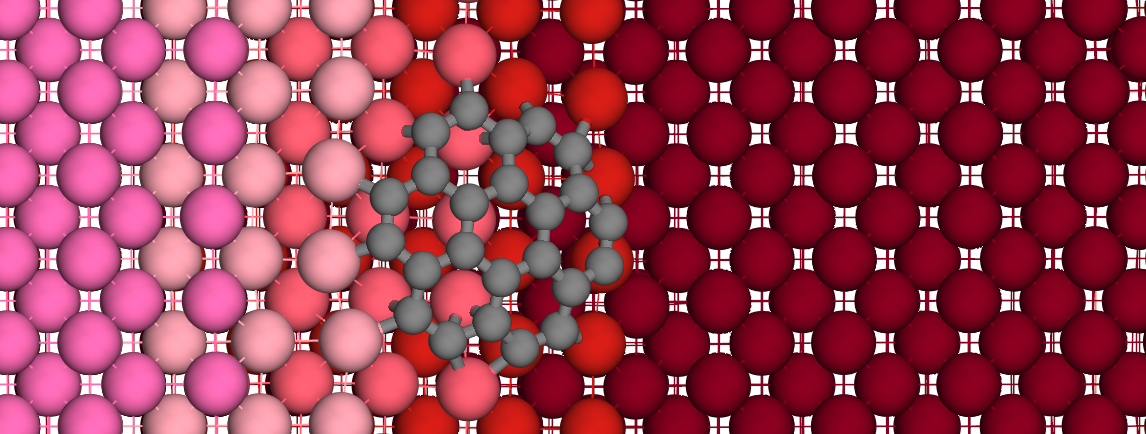
\includegraphics[width=0.4\textwidth,trim=80 0 150 0,clip]{pic/GO_113_structure_top.png}
    }
    \\
%\end{figure}
%\begin{figure}[ht]\ContinuedFloat
    \subfloat[]{
        \label{fig:GO_113_structure_energy}
        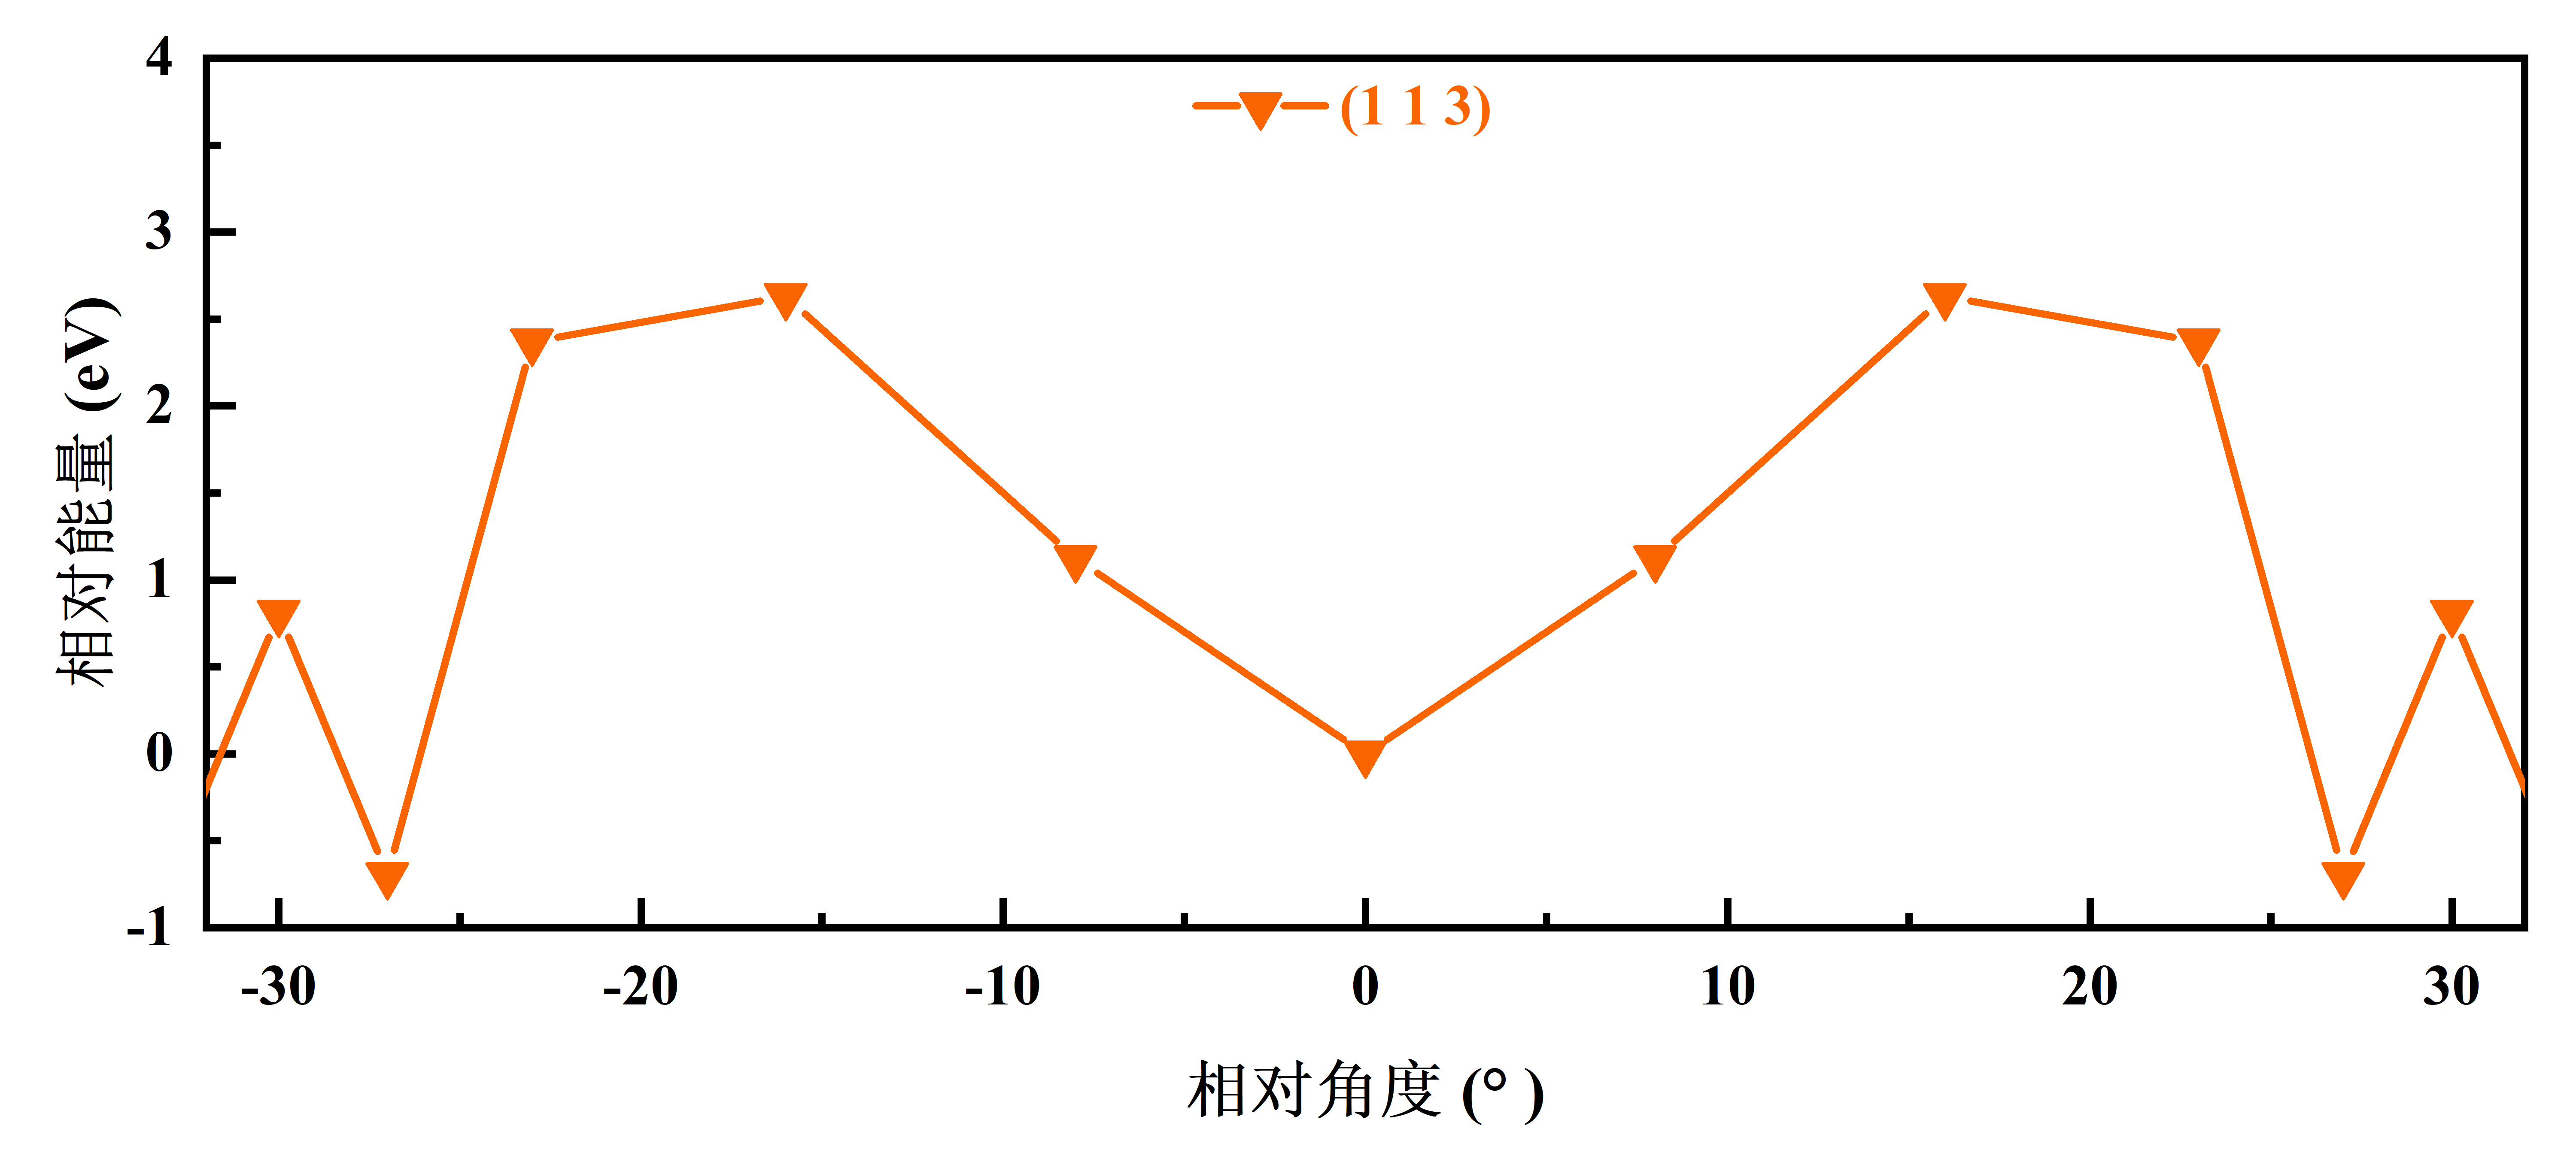
\includegraphics[width=0.8\textwidth]{pic/GO_C24_113_energy.png}
    }
    \caption{\cemb{Cu(113)}晶面上石墨烯$\CCluster{24}$团簇的最优生长晶向($\SI{\pm 270}{\degree}$)、原子构型以及各生长角度能量分布图。(a)原子构型侧视图;(b)原子构型俯视图;(c)各生长角度能量分布。图中,\cemb{C}原子为灰色,\cemb{Cu}原子为红色,不同层的\cemb{Cu}原子以不同亮度进行区分}
    \label{GO_C24_113}
\end{figure}


图\ref{fig:GO_C24_energyDiff_barrier}和表\ref{tab:GO_energyDiff_barrier}中总结了(11n) ($\rm{n \geqslant 1}$)这一系列的\cemb{Cu}衬底上石墨烯$\CCluster{24}$团簇的定向生长能量指标。

\begin{figure}[htb]
    \includegraphics[width=0.8\textwidth]{pic/GO_C24_energyDiff_barrier.png}
    \caption{$\CCluster{24}$团簇在不同衬底表面的次优-最优生长角度能量差(点)和旋转势垒(柱)。图中,能够实现定向生长的衬底以黑点标识,无法实现定向生长的衬底以黑红点标识}
    \label{fig:GO_C24_energyDiff_barrier}
\end{figure}

在能够实现$\CCluster{24}$团簇定向生长的衬底中,\cemb{Cu(115)}晶面具有最高的最优-次优生长角度能量差值,为$\SI{0.64 }{\electronvolt}$。根据热力学的统计定律,可以计算$\CCluster{24}$团簇在热平衡状态下处于最优生长角度和次优生长角度的比例$r$如式\eqref{eq:GO_angleRate}所示\chinesecolon
\begin{equation}
    \label{eq:GO_angleRate}
    r=e^{-\frac{\rm{\Delta} \it E}{k_{\rm B}T}}
\end{equation}
其中$\rm{\Delta} \it E$为两个态之间的能量差,$k_{\rm B}$为玻尔兹曼常数,$T$为温度。对于$\CCluster{24}$团簇在\cemb{Cu(115)}晶面的成核生长,取温度$T$为常见的化学气相沉积生长石墨烯的温度$\SI{1300 }{\kelvin}$,可以计算得出$\CCluster{24}$团簇处于处于最优生长角度和次优生长角度的比例$r\approx 0.0037$。即在热平衡状态写只有不到$\SI{0.4}{\percent}$的石墨烯$\CCluster{24}$团簇处于非定向生长的状态。而对于最优-次优生长角度差值较低的\cemb{Cu(112)}晶面,同样计算可得$\CCluster{24}$团簇在其上生长的角度比例$r\approx 0.053$。相比于\cemb{Cu(115)}面,\cemb{Cu(112)}面的非定向石墨烯畴的比例上升了一个数量级。


进一步考虑$\CCluster{24}$团簇在不同衬底表面从次优生长角度转变至最优生长角度的旋转势垒。在能够实现$\CCluster{24}$团簇定向生长的衬底中,\cemb{Cu(112)}晶面具有最低的旋转势垒,为$\SI{1.57 }{\electronvolt}$。\cemb{Cu(115)}面紧随其后,为$\SI{2.03 }{\electronvolt}$。更低的旋转势垒可以使$\CCluster{24}$团簇更快得达到热平衡的状态。

综合考虑最优-次优能量差和旋转势垒的情况,可以发现对于(11n) ($\rm{n \geqslant 1}$)这一系列的\cemb{Cu}衬底表面存在台阶,石墨烯在能量上会倾向于在衬底表面台阶的边缘定向生长。虽然\cemb{Cu(113)}台面上不重叠的两个最优生长角度会使得石墨烯呈现出不定向生长的趋势,但是由于(113)台面非常高表面能\citing{RN1063-1993},在实际生长过程中的占比很小。可以认为可以使用基于(11n) ($\rm{n \geqslant 1}$)这一系列的指数的多晶\cemb{Cu}衬底,尤其是指数接近\cemb{Cu(112)}晶面,能够对多点成核的石墨烯进行自发的定向生长,从而实现高效低成本的大面积单晶石墨烯的制备。通过与实验研究者合作,本小节所阐述的\cemb{Cu}衬底表面台阶边缘石墨烯优先成核、定向生长的机理已被用于在多晶铜衬底表面生长大规模、方向均一的石墨烯畴\citing{RN839-2020}。实验结果显示在接近\cemb{Cu(112)}晶面的\cemb{Cu}衬底表面实现了生长方向高度一致的石墨烯畴,和本小节说述的理论计算结果吻合。

\begin{table}[htb]
    \caption{石墨烯$\CCluster{24}$团簇在\cemb{Cu(11n)} ($\rm{n \geqslant 1}$)衬底上定向生长的最优角度,最优-次优能量差以及旋转势垒}
    \centering
    \begin{tabular}{ccccc}
        \toprule
        \cemb{Cu}晶面指数  & 最优生长角度             & 次优生长角度            & 能量差                       & 旋转势垒 \\
        \midrule
        (001)      & $\SI{\pm 15 }{\degree}$ & 非定向                  & 非定向                      & 非定向                        \\
        (11X)      & $\SI{0}{\degree}$       & $\SI{\pm 30}{\degree}$ & $\SI{0.56 }{\electronvolt}$ & $\SI{2.56 }{\electronvolt}$  \\
        (117)      & $\SI{0}{\degree}$       & $\SI{\pm 30}{\degree}$ & $\SI{0.43 }{\electronvolt}$ & $\SI{2.91 }{\electronvolt}$  \\
        (115)      & $\SI{0}{\degree}$       & $\SI{\pm 30}{\degree}$ & $\SI{0.63 }{\electronvolt}$ & $\SI{2.07}{\electronvolt}$   \\
        (113)      & $\SI{\pm 27}{\degree}$  & $\SI{0}{\degree}$      & 非定向                      & 非定向                        \\
        (112)      & $\SI{0}{\degree}$       & $\SI{\pm 30}{\degree}$ & $\SI{0.33 }{\electronvolt}$ & $\SI{1.57 }{\electronvolt}$  \\
        (111)      & $\SI{\pm 18 }{\degree}$ & 非定向                 & 非定向                       & 非定向                        \\
        \bottomrule
    \end{tabular}
    \label{tab:GO_energyDiff_barrier}
\end{table}

\section{氧通量调控的石墨烯多层点蚀刻/生长的模式切换机制}
\label{sec:石墨烯氧蚀刻穿透}
\def\muO#1{\it \mu_{\rm O}^{\rm #1} \it}
\def\halfEOm{\it \frac{1}{2}E_{\rm \cemb{O2}} \it}
\def\EOa{\it E_{\rm O} \it }
\def\Cdis{\rm{\left[C_{dis.}\right]} \it }
\def\Oads{\rm{\left[O_{ads.}\right]} \it }
\def\RateV#1#2{\it \nu_{\rm #1}^{\rm #2} \it }
\def\RateK#1#2{\it{k_{\rm #1}^{\rm #2}} \it }
\def\ReactTime#1#2{\it{t_{\rm #1}^{\rm #2}} \it }

\subsection{化学气相沉积法制备石墨烯的生长气氛模拟}
\label{subsec:FLG_gasPhase}
当\cemb{Cu}衬底的表面覆盖满石墨烯后,由于\cemb{Cu}衬底的对甲烷的催化作用被已生长的石墨烯阻挡,此时石墨烯的生长表现出自限制的效应,使石墨烯保持单层的形貌。因此,当要在覆盖满石墨烯的\cemb{Cu}衬底上继续生长双层乃至于多层石墨烯,生长气氛中的甲烷的化学反应动力学过程就变得尤为重要。已有研究者证明,氧气的加入会促进甲烷在气相过程中的裂解,有利于石墨烯第二层的生长\citing{RN1052-2016}。为了进一步探究氧气的引入对于化学气相沉积石墨烯多层的影响。本小节利用气相动力学模拟的方法,对引入氧气的常压化学气相沉积系统(APCVD)中反应气氛中的化学反应以及相应的化学物质的浓度分布进行了计算。

首先,本小节对化学气相沉积过程中石墨烯生长位点的化学组分随时间分布的浓度变化情况进行了模拟仿真(图\ref{fig:FLG_fluent})。依照实验中的生长参数,设定氩氧混合气体的流量为$\SI{120}{SCCM}$。其中氩氧混合气中的氧气浓度比例为$\SI{0.4}{\percent}$。模拟环境中其他输入气体的流量参数为$\SI{8}{SCCM}$的纯氢气,$\SI{20}{SCCM}$的甲烷氩气混合气体(其中甲烷的浓度比例为$\SI{1}{\percent}$)以及$\SI{300}{SCCM}$的纯氩气。以含氧混合气体通入反应炉的时间作为模拟的开始时间$\SI{0}{\second}$,反应炉中的生长气氛的初始状态为只含有纯氩气的保护气氛。

\begin{figure}[htb]
    \centering
    \subfloat[]{
        \label{fig:FLG_fluent_C_molConcen}
        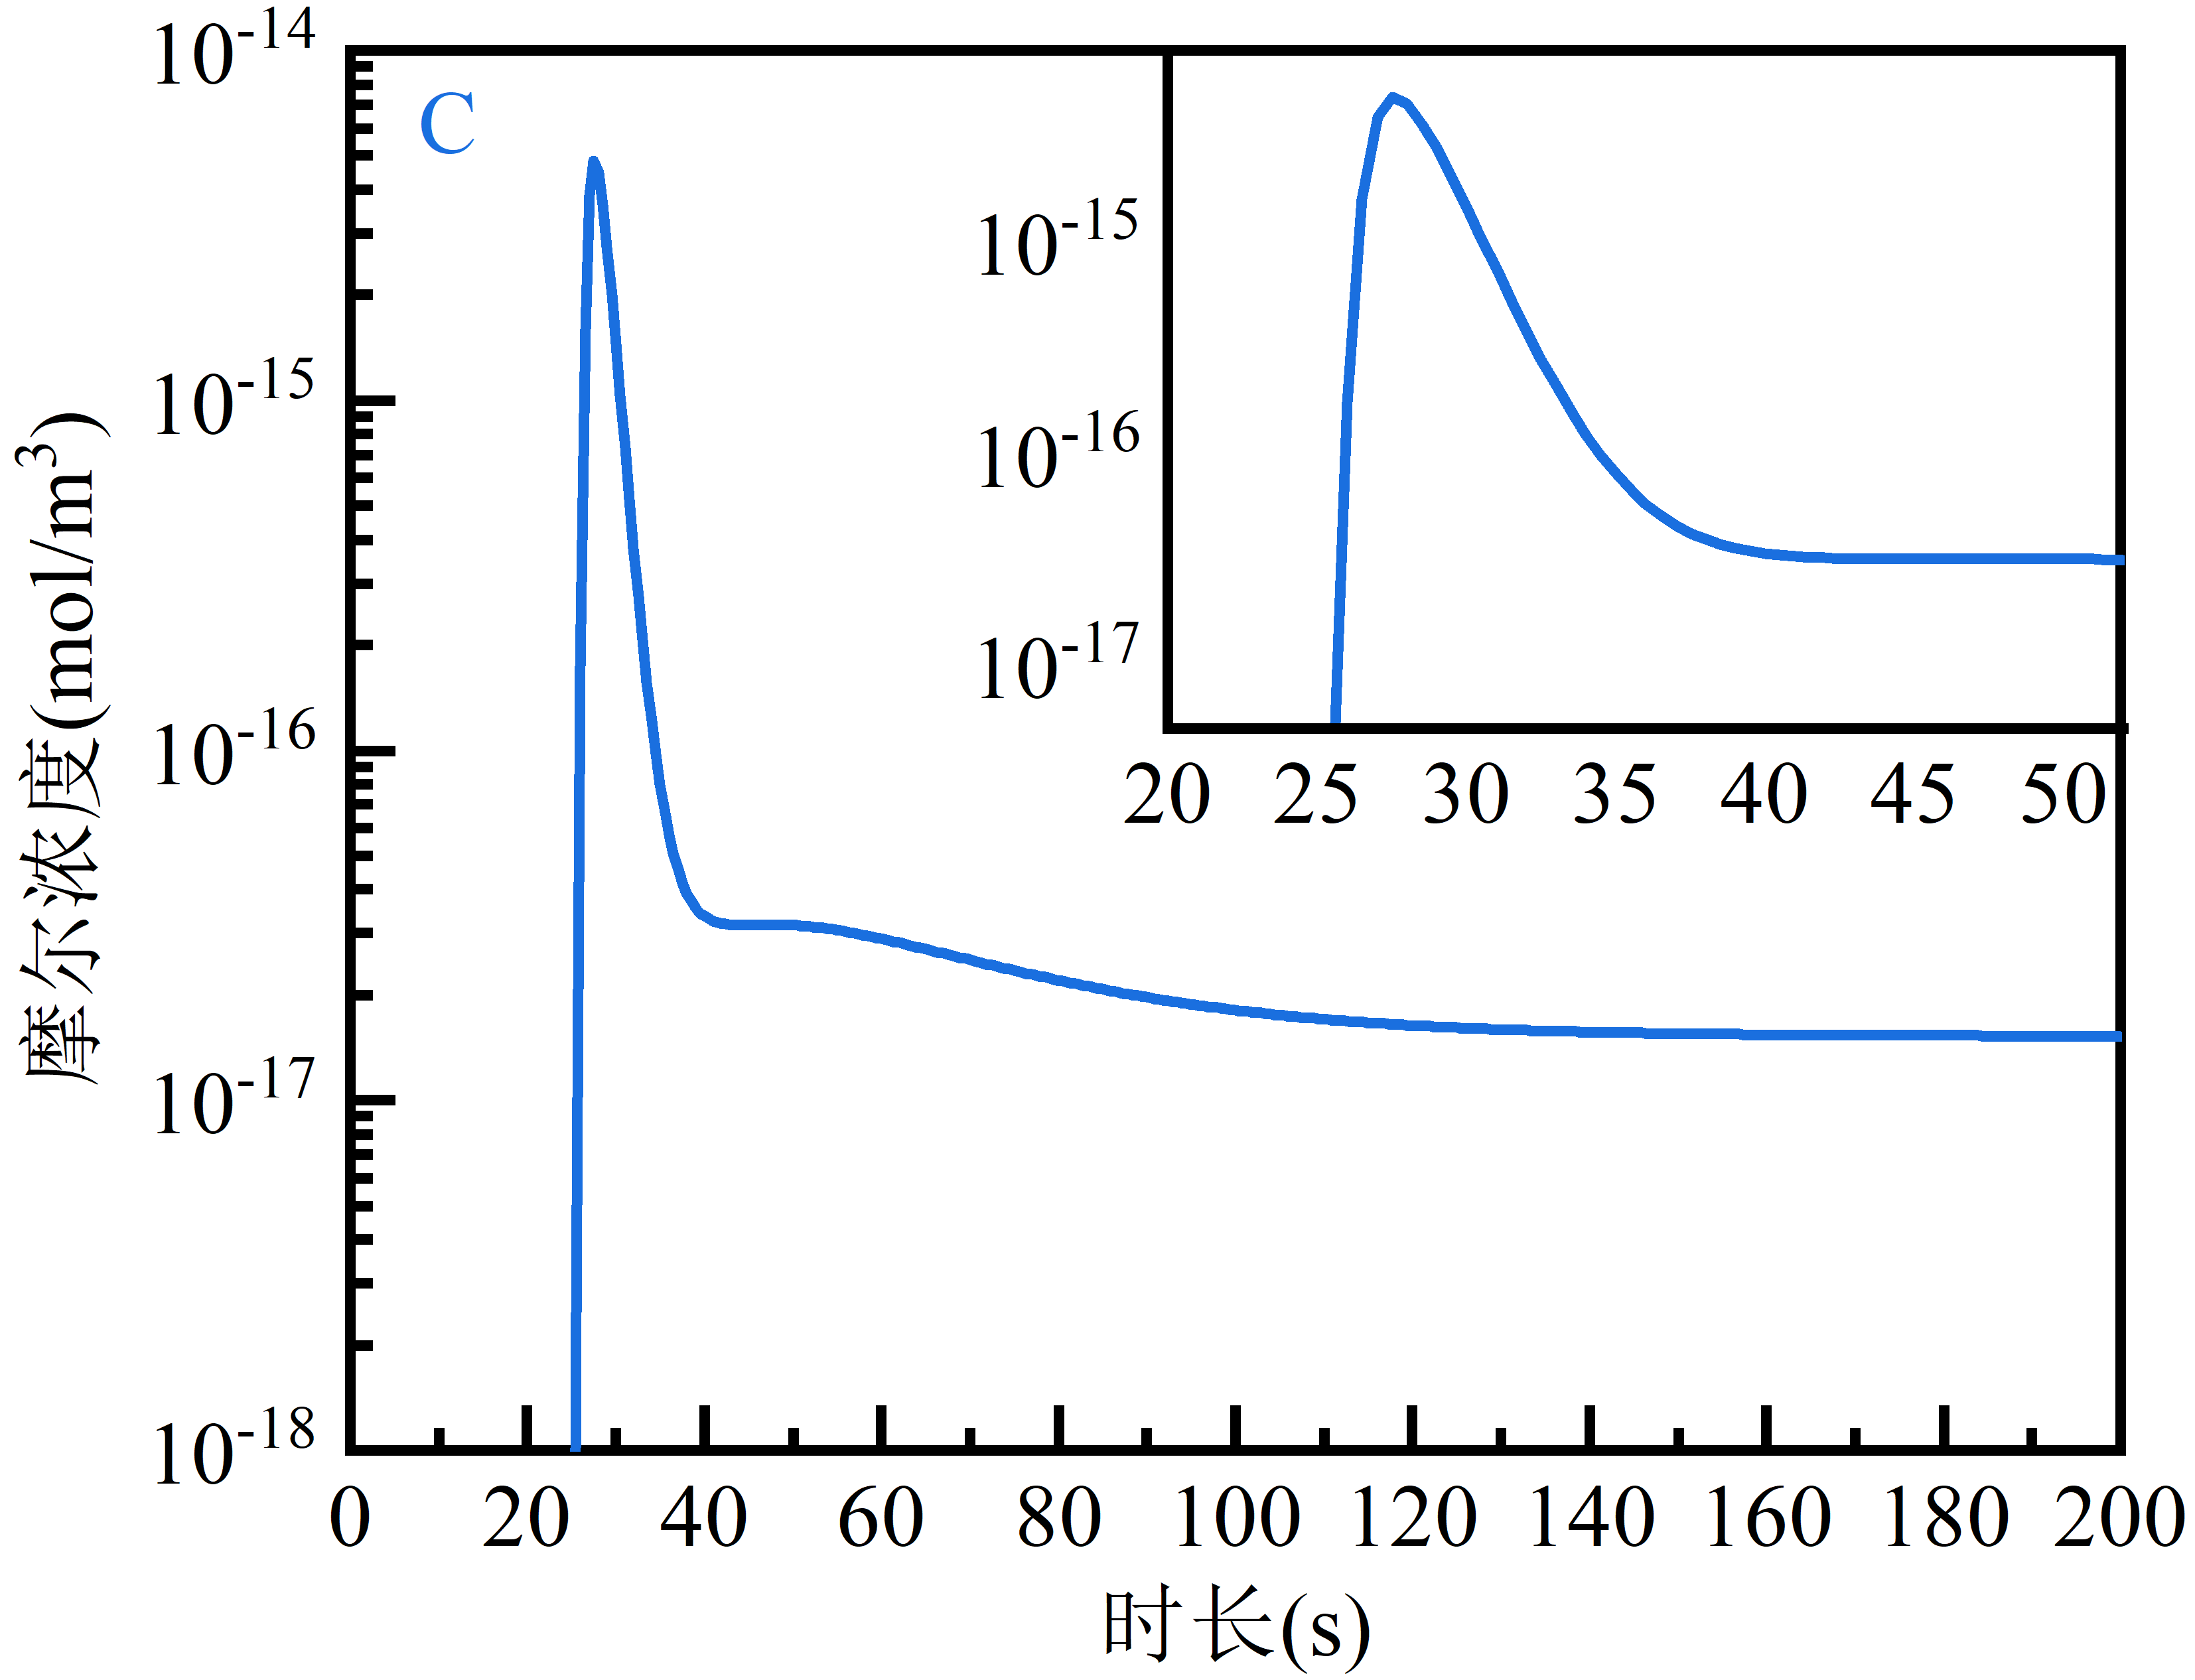
\includegraphics{pic/FLG_fluent_C_molConcen.png}
    }
    \subfloat[]{
        \label{fig:FLG_fluent_O_molConcen}
        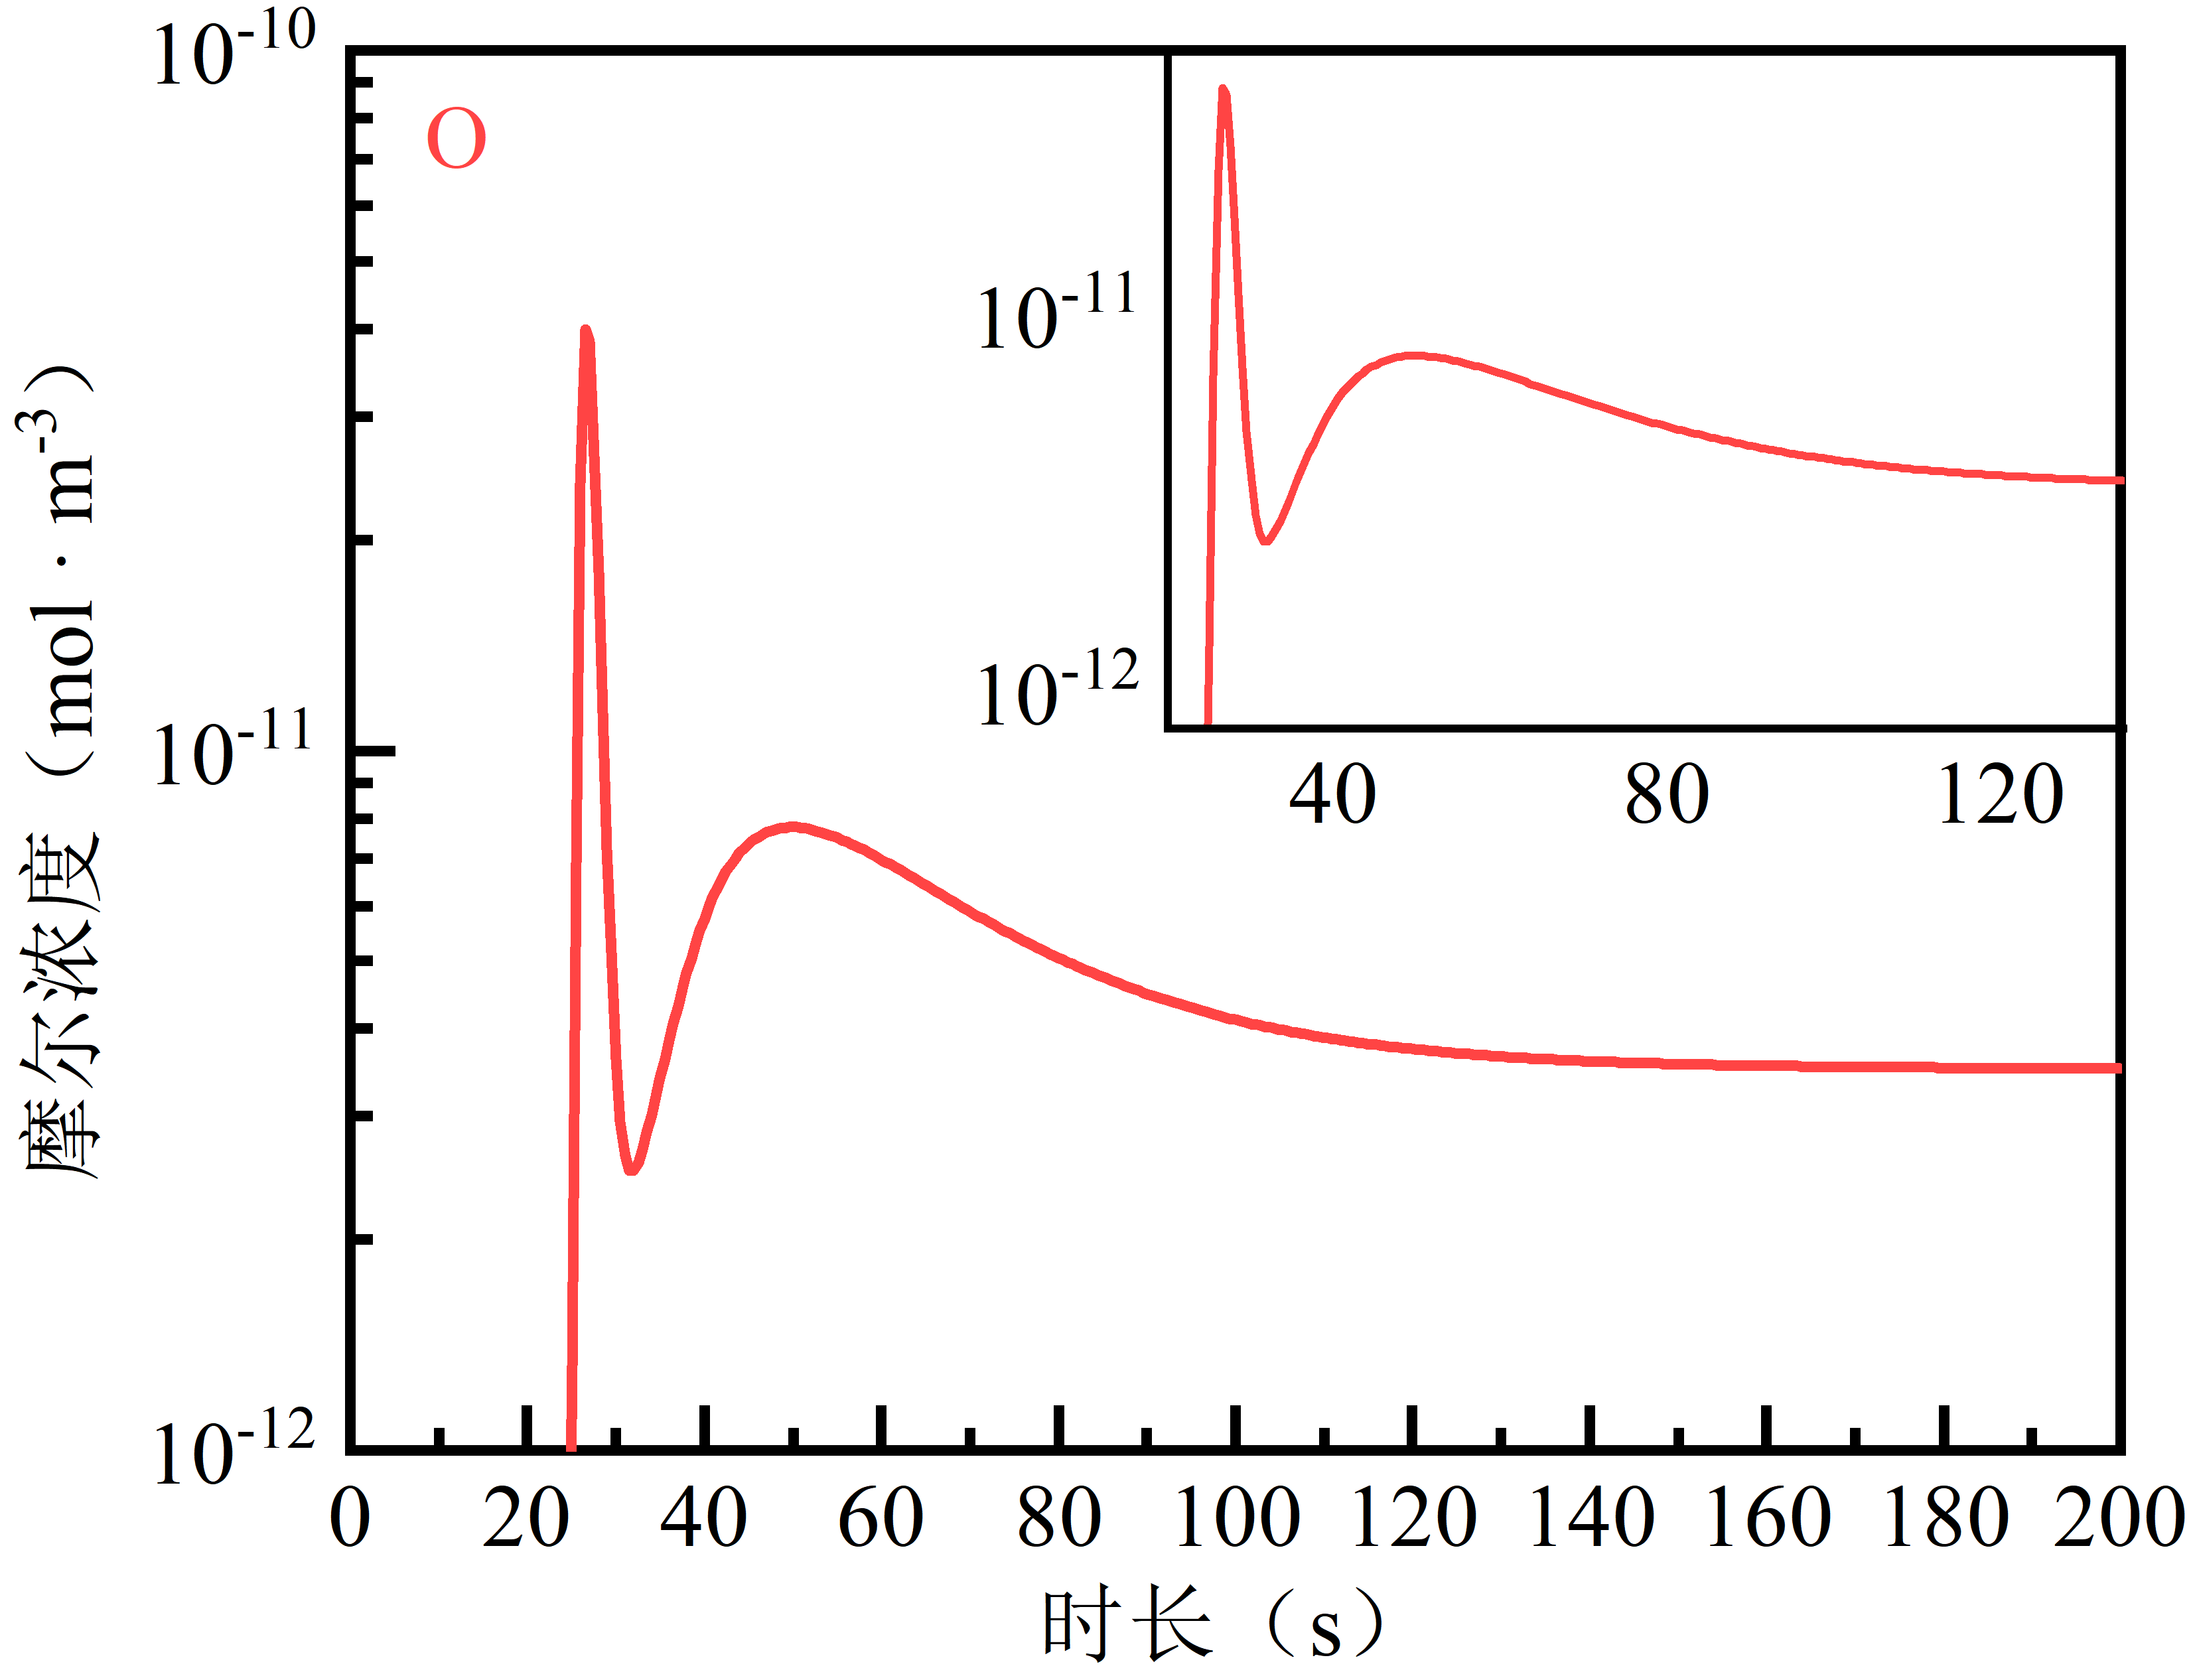
\includegraphics{pic/FLG_fluent_O_molConcen.png}
    }\\
    \subfloat[]{
        \label{fig:FLG_fluent_O-C_ratio}
        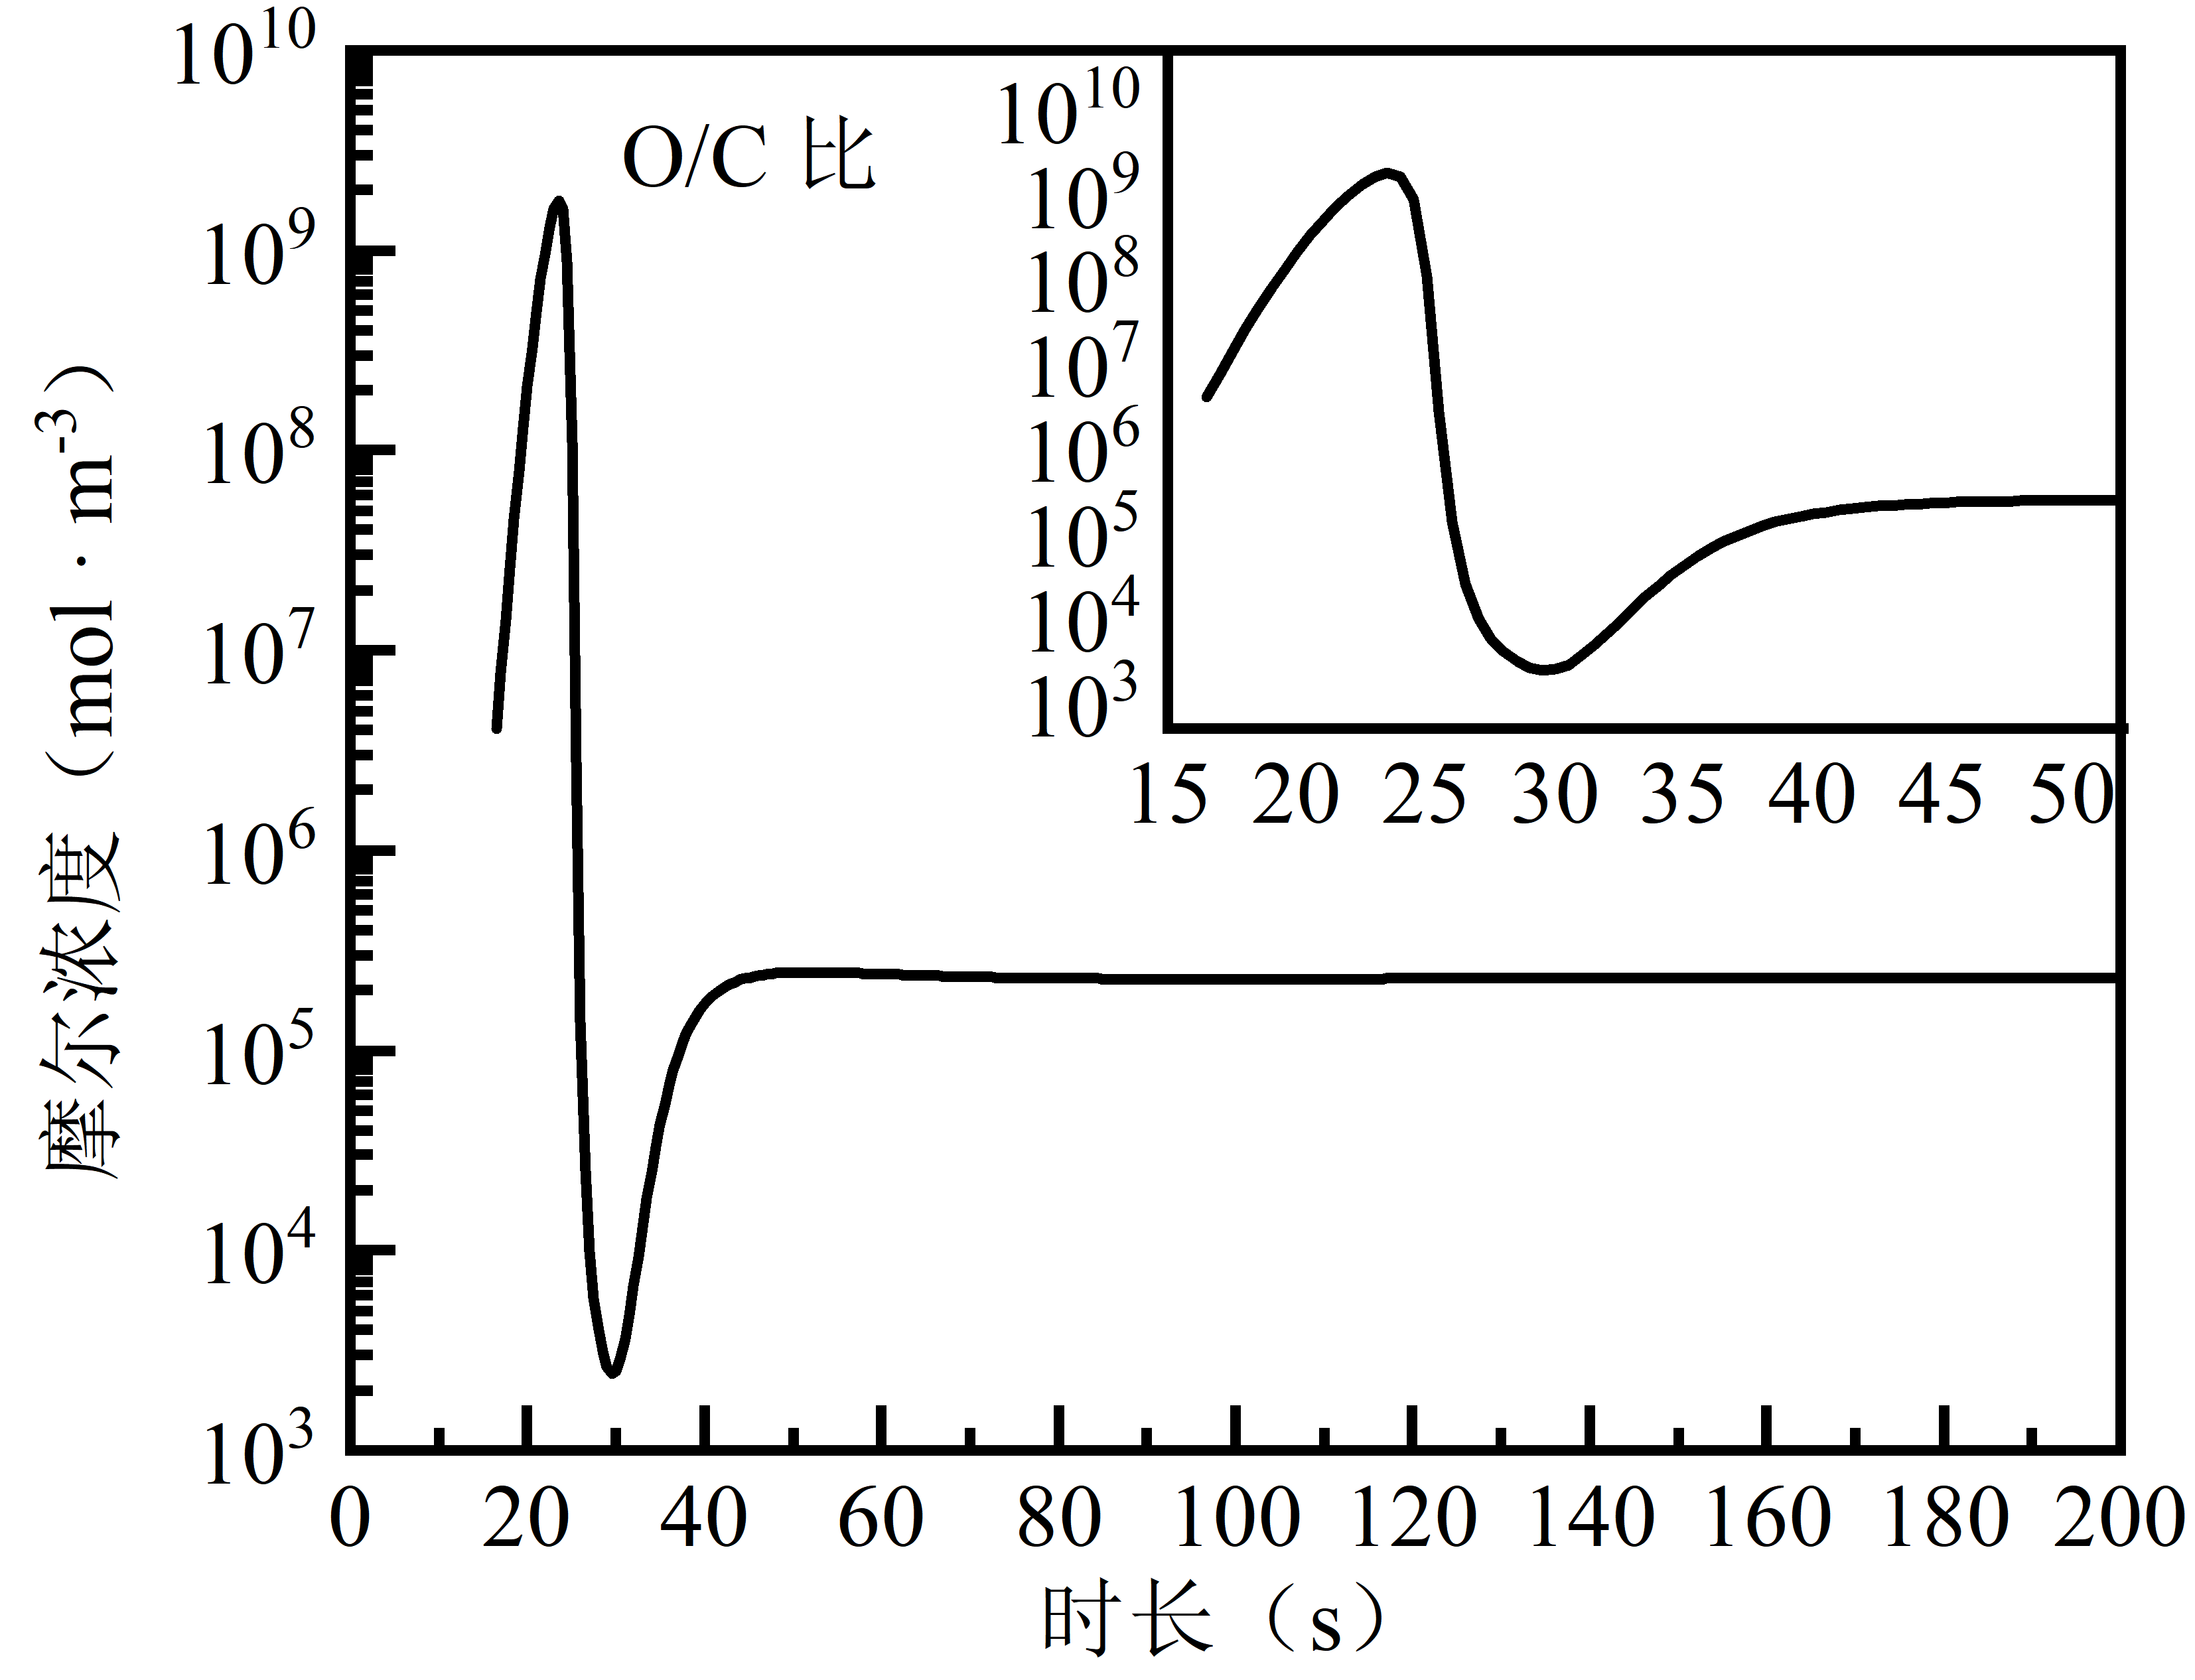
\includegraphics{pic/FLG_fluent_O-C_ratio.png}
    }
    \caption{化学气相沉积过程中石墨烯生长位点的化学组分随时间分布的浓度变化。(a)C自由基浓度;(b)O自由基浓度;(c)O/C比例。}
    \label{fig:FLG_fluent}
\end{figure}

使用反应活性最高的C自由基和O自由基作为生长气氛中直接参与石墨烯生长和蚀刻反应的代表反应物。在常压化学气相沉积的系统内,输入氧气后大约\SI{25}{\second}之后,在石墨烯生长位点开始有明显的甲烷分解反应发生。对于C自由基而言,由于氧气参与并促进甲烷的裂解反应,C自由基的浓度极速上升,最高浓度可达$\SI{4e-15}{\mole\per\cubic\metre}$。随后由于\cemb{CO}以及\cemb{CO2}等碳氧化物的生成,C自由基的浓度迅速下降,并在约第\SI{40}{\second}后C自由基的浓度稳定在$\SI{1e-17}{\mole\per\cubic\metre}$附近。而对于O自由基,情况则更为复杂。在$\SI{25}{\second}$时,氧气经过气体输运到达石墨烯生长位点,被迅速加热开始分解成为\cemb{O}自由基。此时\cemb{O}自由基的最高浓度最高可达$\SI{3e-11}{\mole\per\cubic\metre}$。随后由于参与甲烷裂解和与氢气的化合反应,\cemb{O}自由基的浓度下降至$\SI{2e-12}{\mole\per\cubic\metre}$并在$\SI{3e-12}{\mole\per\cubic\metre}$附近产生震荡。\cemb{O}自由基浓度震荡在约$\SI{50}{\second}$处到达最高值$\SI{8e-12}{\mole\per\cubic\metre}$并逐渐回落至$\SI{3e-12}{\mole\per\cubic\metre}$。考虑到在石墨烯的生长过程中以C自由基和O自由基为代表的活性物质对于石墨烯的生长和蚀刻作用是同时进行的,可以使用O/C比来考察化学气相沉积过程中通入氩氧混合气后生长气氛中的化合物达到平衡状态所需的时间(图\ref{fig:FLG_fluent_O-C_ratio})。在O/C比在通入氩氧混合气的第\SI{45}{\second}后就基本趋于稳定。考虑到实验中生长多层石墨烯通常需要几十分钟乃至几个小时的时间,因此可以认为在生长气氛中引入氧气的情况下,石墨烯生长和蚀刻反应所涉及的化学气氛均已达到稳态。因此,为了考察不同氧气通入量对于石墨烯生长的影响,接下来的计算中将采用更加快速高效的稳态计算方法对石墨烯的生长气氛进行模拟。

图\ref{fig:FLG_chemkin}展示了通入不同流量的氧气情况下石墨烯生长位点的化学组分浓度情况。为了探究前驱体中不同氧气含量对多层石墨烯生长的影响,图\ref{fig:FLG_chemkin}囊括了氩氧混合气输入的流量从$\SI{0}{SCCM}$增加到$\SI{500}{SCCM}$后,石墨烯生长气氛中的气相化学反应和相应稳态下反应物的浓度分布情况。

\begin{figure}[htb]
    \subfloat[]{
        \label{fig:FLG_chemkin_full}
        \includegraphics[width=0.48\textwidth]{pic/FLG_chemkin_full.png}
    }
    \subfloat[]{
        \label{fig:FLG_chemkin_part}
        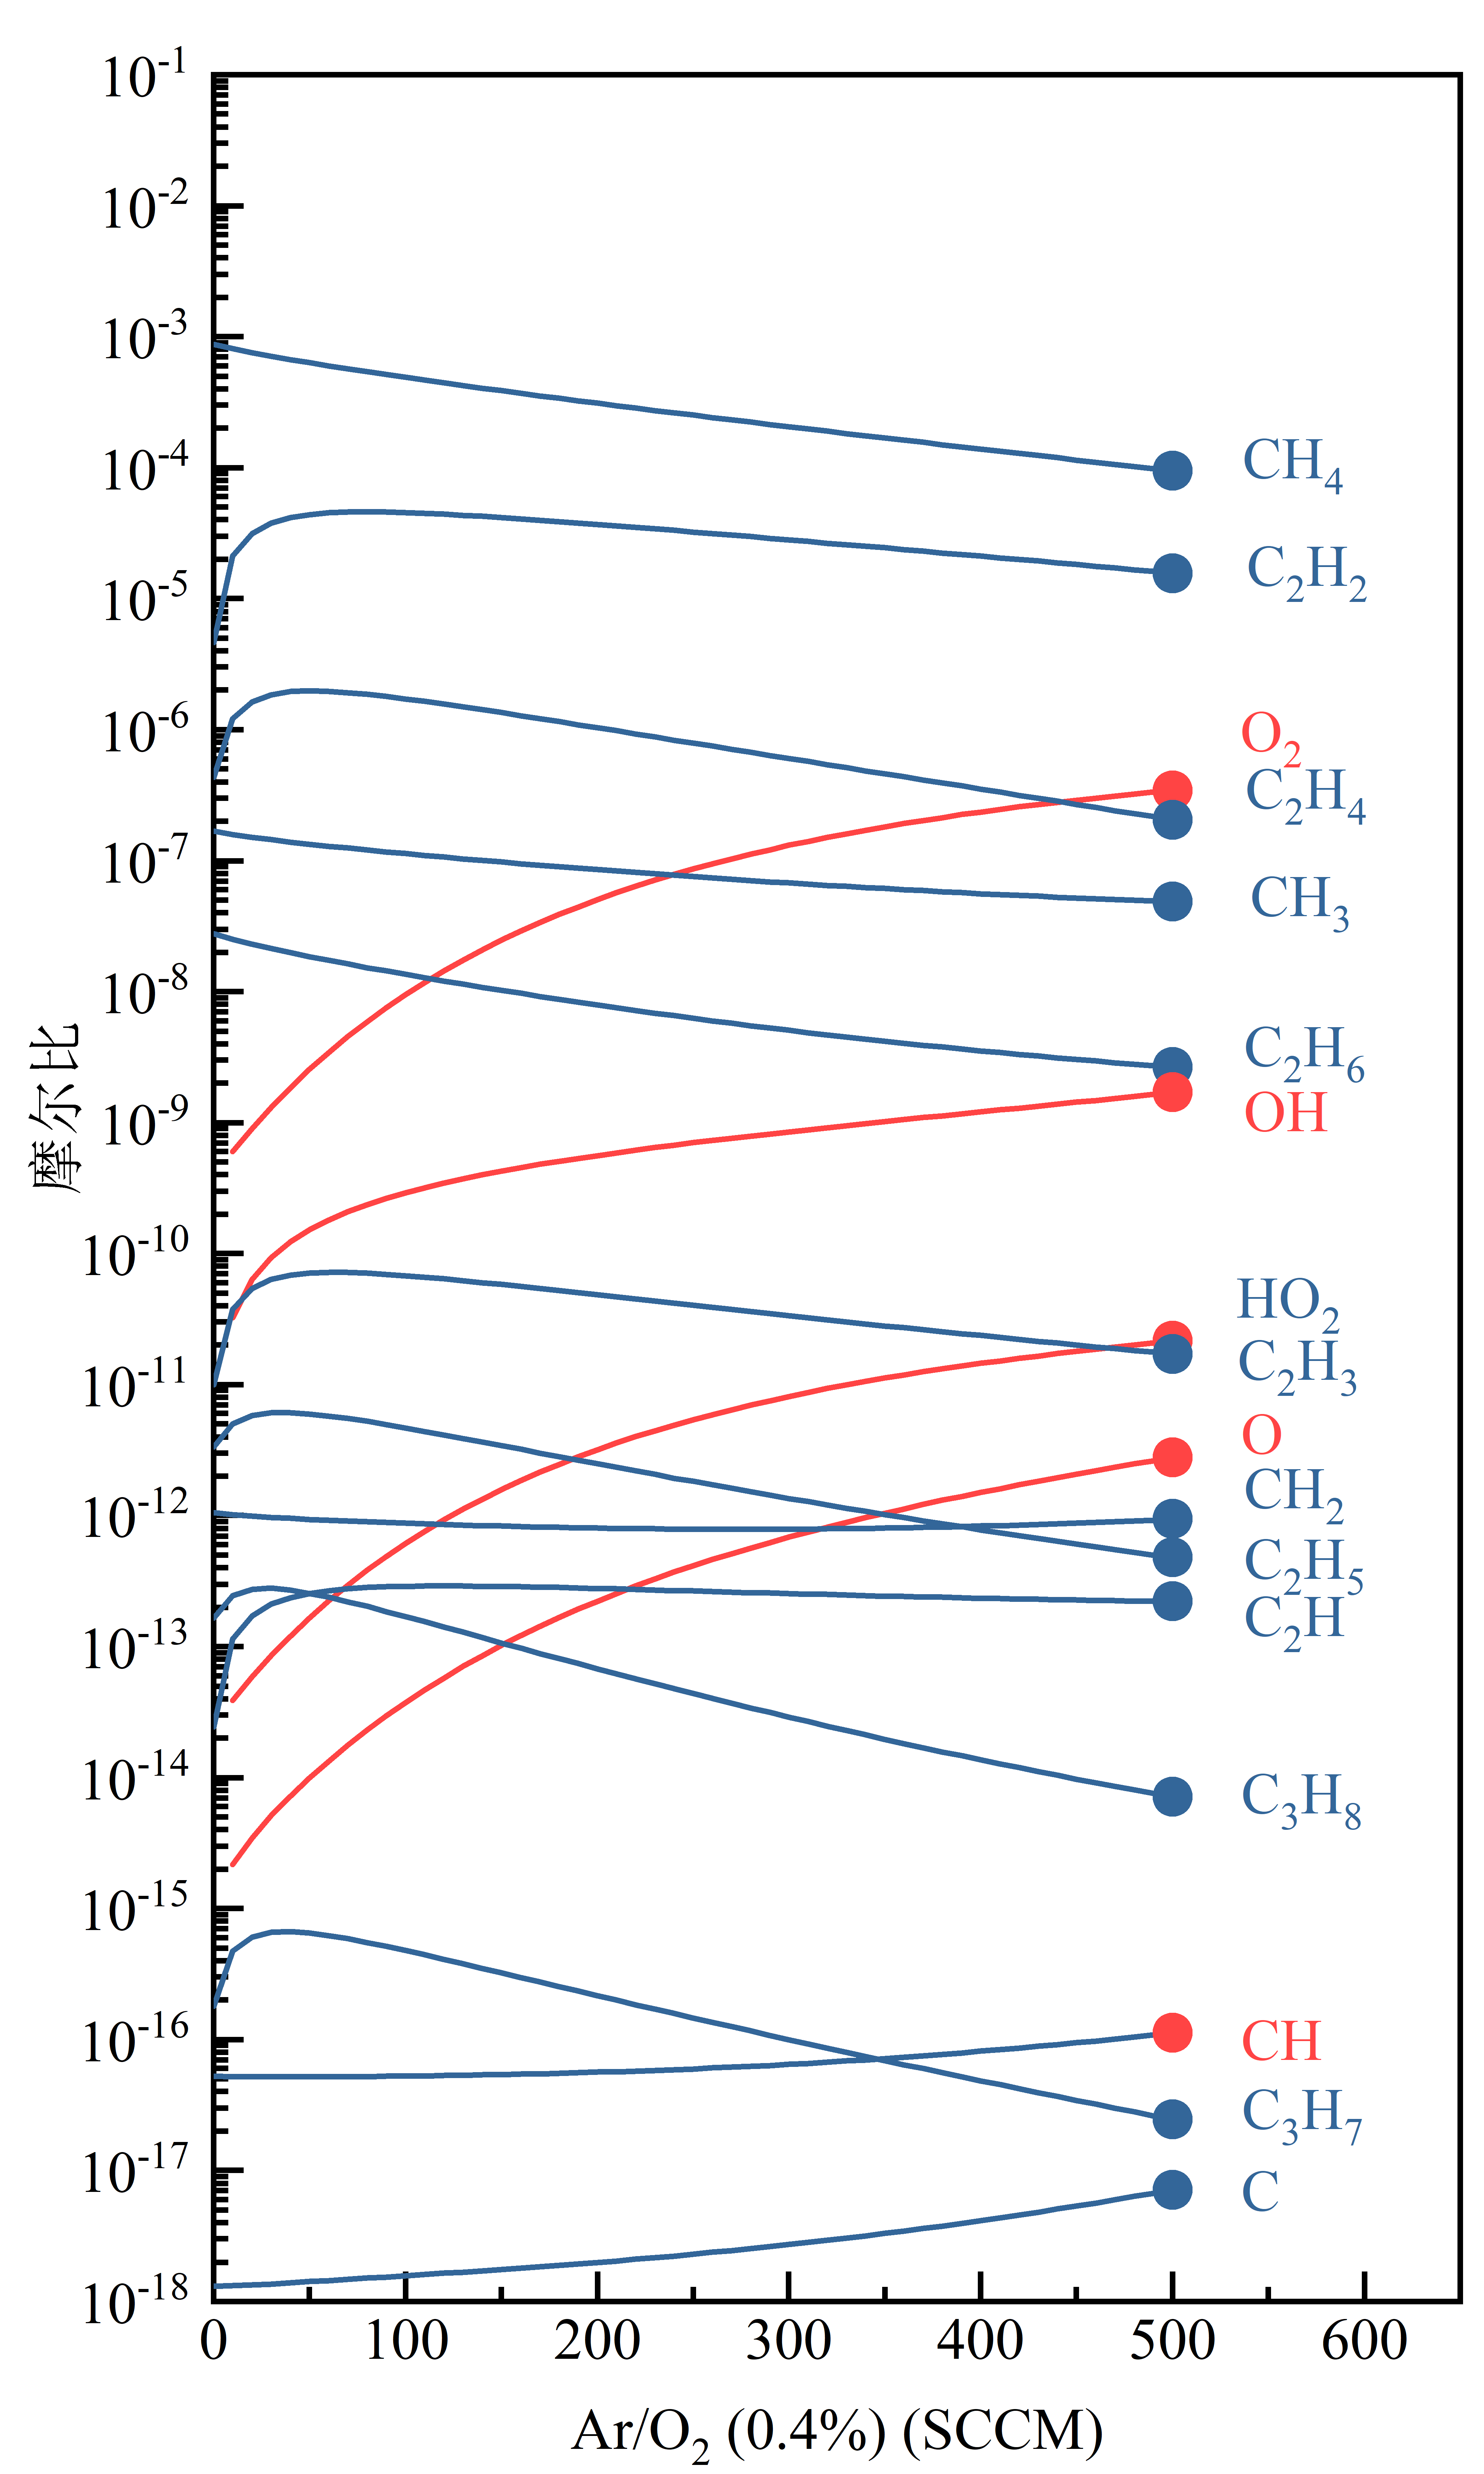
\includegraphics[width=0.48\textwidth]{pic/FLG_chemkin_part.png}
    }
    \caption{生长环境中化学组分浓度分布随着通入氧气流量大小的变化情况。(a)模拟中涉及的所有化合物的浓度分布情况;(b)石墨烯蚀刻物质与生长物质的浓度分布情况}
    \label{fig:FLG_chemkin}
\end{figure}

整体来看,随着通入氧气流量的上升,甲烷的裂解程度也随之上升。甲烷与氧气反应生成大量的一氧化碳和二氧化碳以及种类众多的碳氢氧化合物。而碳氢化合物的浓度随着氧气通入流量的上升呈现出先上升后下降的趋势。氢气的浓度随着更多氧气的通入逐渐下降,但活性氢原子的浓度保持在一个非常稳定的区间。
为了简化分析,在氢-氧-甲烷反应所涉及的所有物质中,在本节的研究中主要关注那些能够蚀刻石墨烯以及能够为石墨烯生长提供碳源的化合物(图\ref{fig:FLG_chemkin_part})。其中,在本章中所考虑的蚀刻物质包括\cemb{O}自由基、氢氧化物和氧气,生长物质包括活性炭自由基,碳氢化合物等。

对于蚀刻物质,计算发现随着氧气通入量的上升,\cemb{O}、\cemb{OH}以及$\cemb{HO2}$的浓度急剧上升。以\cemb{O}自由基为例,活性\cemb{O}自由基的浓度在氩氧混合气的输入流量为$\SI{5}{SCCM}$时约为$\SI{2e-15}{}$。在氩氧混合气的输入流量为$\SI{500}{SCCM}$时,\cemb{O}自由基在气氛中的浓度提升至$\SI{3e-2}{}$,大约提升了三个数量级。而对于$\cemb{OH}$和$\cemb{HO2}$,二者的浓度随着氩氧混合气的输入流量的上升也有两到三个数量级的浓度提升。

而气氛中的生长物质随着氧气通入量的上升呈现出了了非单调的变化。氧气能够促进甲烷的裂解反应,因此气氛中的C和CH的浓度得以缓慢上升,作为甲烷裂解反应物和中间产物的$\cemb{CH4}$,$\cemb{CH3}$,$\cemb{CH2}$则缓慢下降。而其他碳氢化合物在氧气通入量逐渐上升的情况下大部分呈现出先上升后下降的浓度趋势。
\subsection{氧辅助石墨烯多层点的交换蚀刻作用}
\label{subsec:FLG_Oetch}

考虑到蚀刻物质中$\cemb{O}$、$\cemb{OH}$、$\cemb{HO2}$以及$\cemb{O2}$等物质都对石墨烯具有一定的蚀刻作用,且各蚀刻物质之间的浓度较为接近。为了探究石墨烯在含氧化学气相沉积环境下的蚀刻过程,可以在本节的研究中引入氧原子的化学势$\muO{}$来代表生长气氛中蚀刻物质的整体反应活性。因此,化学势$\muO{}$的变化范围为$\halfEOm$ 至 $\EOa$,对应于氧原子在氧气分子($\cemb{O2}$)内的能级水平和氧原子在\cemb{O}自由基($\cemb{O}$)中的能级水平。随着在蚀刻石墨烯的反应中涉及的高活性蚀刻物质(如\cemb{O}自由基O)浓度的上升,化学势$\muO{}$逐渐上升并接近$\EOa$,同时伴随着更多的石墨烯被蚀刻。

随后,利用密度泛函理论,在$\muO{}$的框架内利用式\eqref{eq:FLG_etchEnergy}计算了氧原子蚀刻石墨烯的反应能$\rm{\Delta} \it E$。
\begin{equation}
    \label{eq:FLG_etchEnergy}
    \rm{\Delta} \it E = E_{\rm product} - E_{\rm initial} - \muO{}
\end{equation}
其中,$E_{\rm product}$和 $E_{\rm initial}$分别为各反应步骤中生成物和反应物的能量。

在以\cemb{Cu}为衬底的化学气相沉积石墨烯生长法中,当\cemb{Cu}的表面被单层的石墨烯覆盖满后,石墨烯多层的生长由于自限制效应而趋近于停止。此时的石墨烯-\cemb{Cu}衬底界面处存在大量的游离碳。这些游离碳在石墨烯-\cemb{Cu}衬底的界面处扩散,成核,形成少量的石墨烯多层点。从热力学的角度看,石墨烯多层点的大小于游离碳的浓度$\Cdis$处于平衡状态。当游离碳的浓度$\Cdis$上升时,处于石墨烯-\cemb{Cu}衬底的界面处的石墨烯多层点的成核密度上升,面积扩大。当游离碳的浓度$\Cdis$下降时,石墨烯多层点开始分解,面积缩小。

从密度泛函理论的计算结果来看(图\ref{fig:FLG_DFT_Oetch}),无论有无游离碳,氧原子都可以在石墨烯上吸附,并且吸附的反应能相近。对于氧气来说,由于在石墨烯上吸附需要进行裂解,因此当$\muO{}=\halfEOm$时,氧原子在界面游离碳上方的石墨烯上的吸附能约为$\SI{-0.35}{\electronvolt}$,在纯石墨烯的表面吸附能约为$\SI{-0.28}{\electronvolt}$。而对于\cemb{O}自由基而言,其可以在石墨烯上直接吸附,相应的吸附步骤的反应能也会下降很多。计算显示当$\muO{}=\EOa$时,氧原子在界面游离碳上方的石墨烯上的吸附能约为$\SI{-3.63}{\electronvolt}$,在纯石墨烯上的吸附能约为$\SI{-3.56}{\electronvolt}$。

\begin{figure}[htb]
    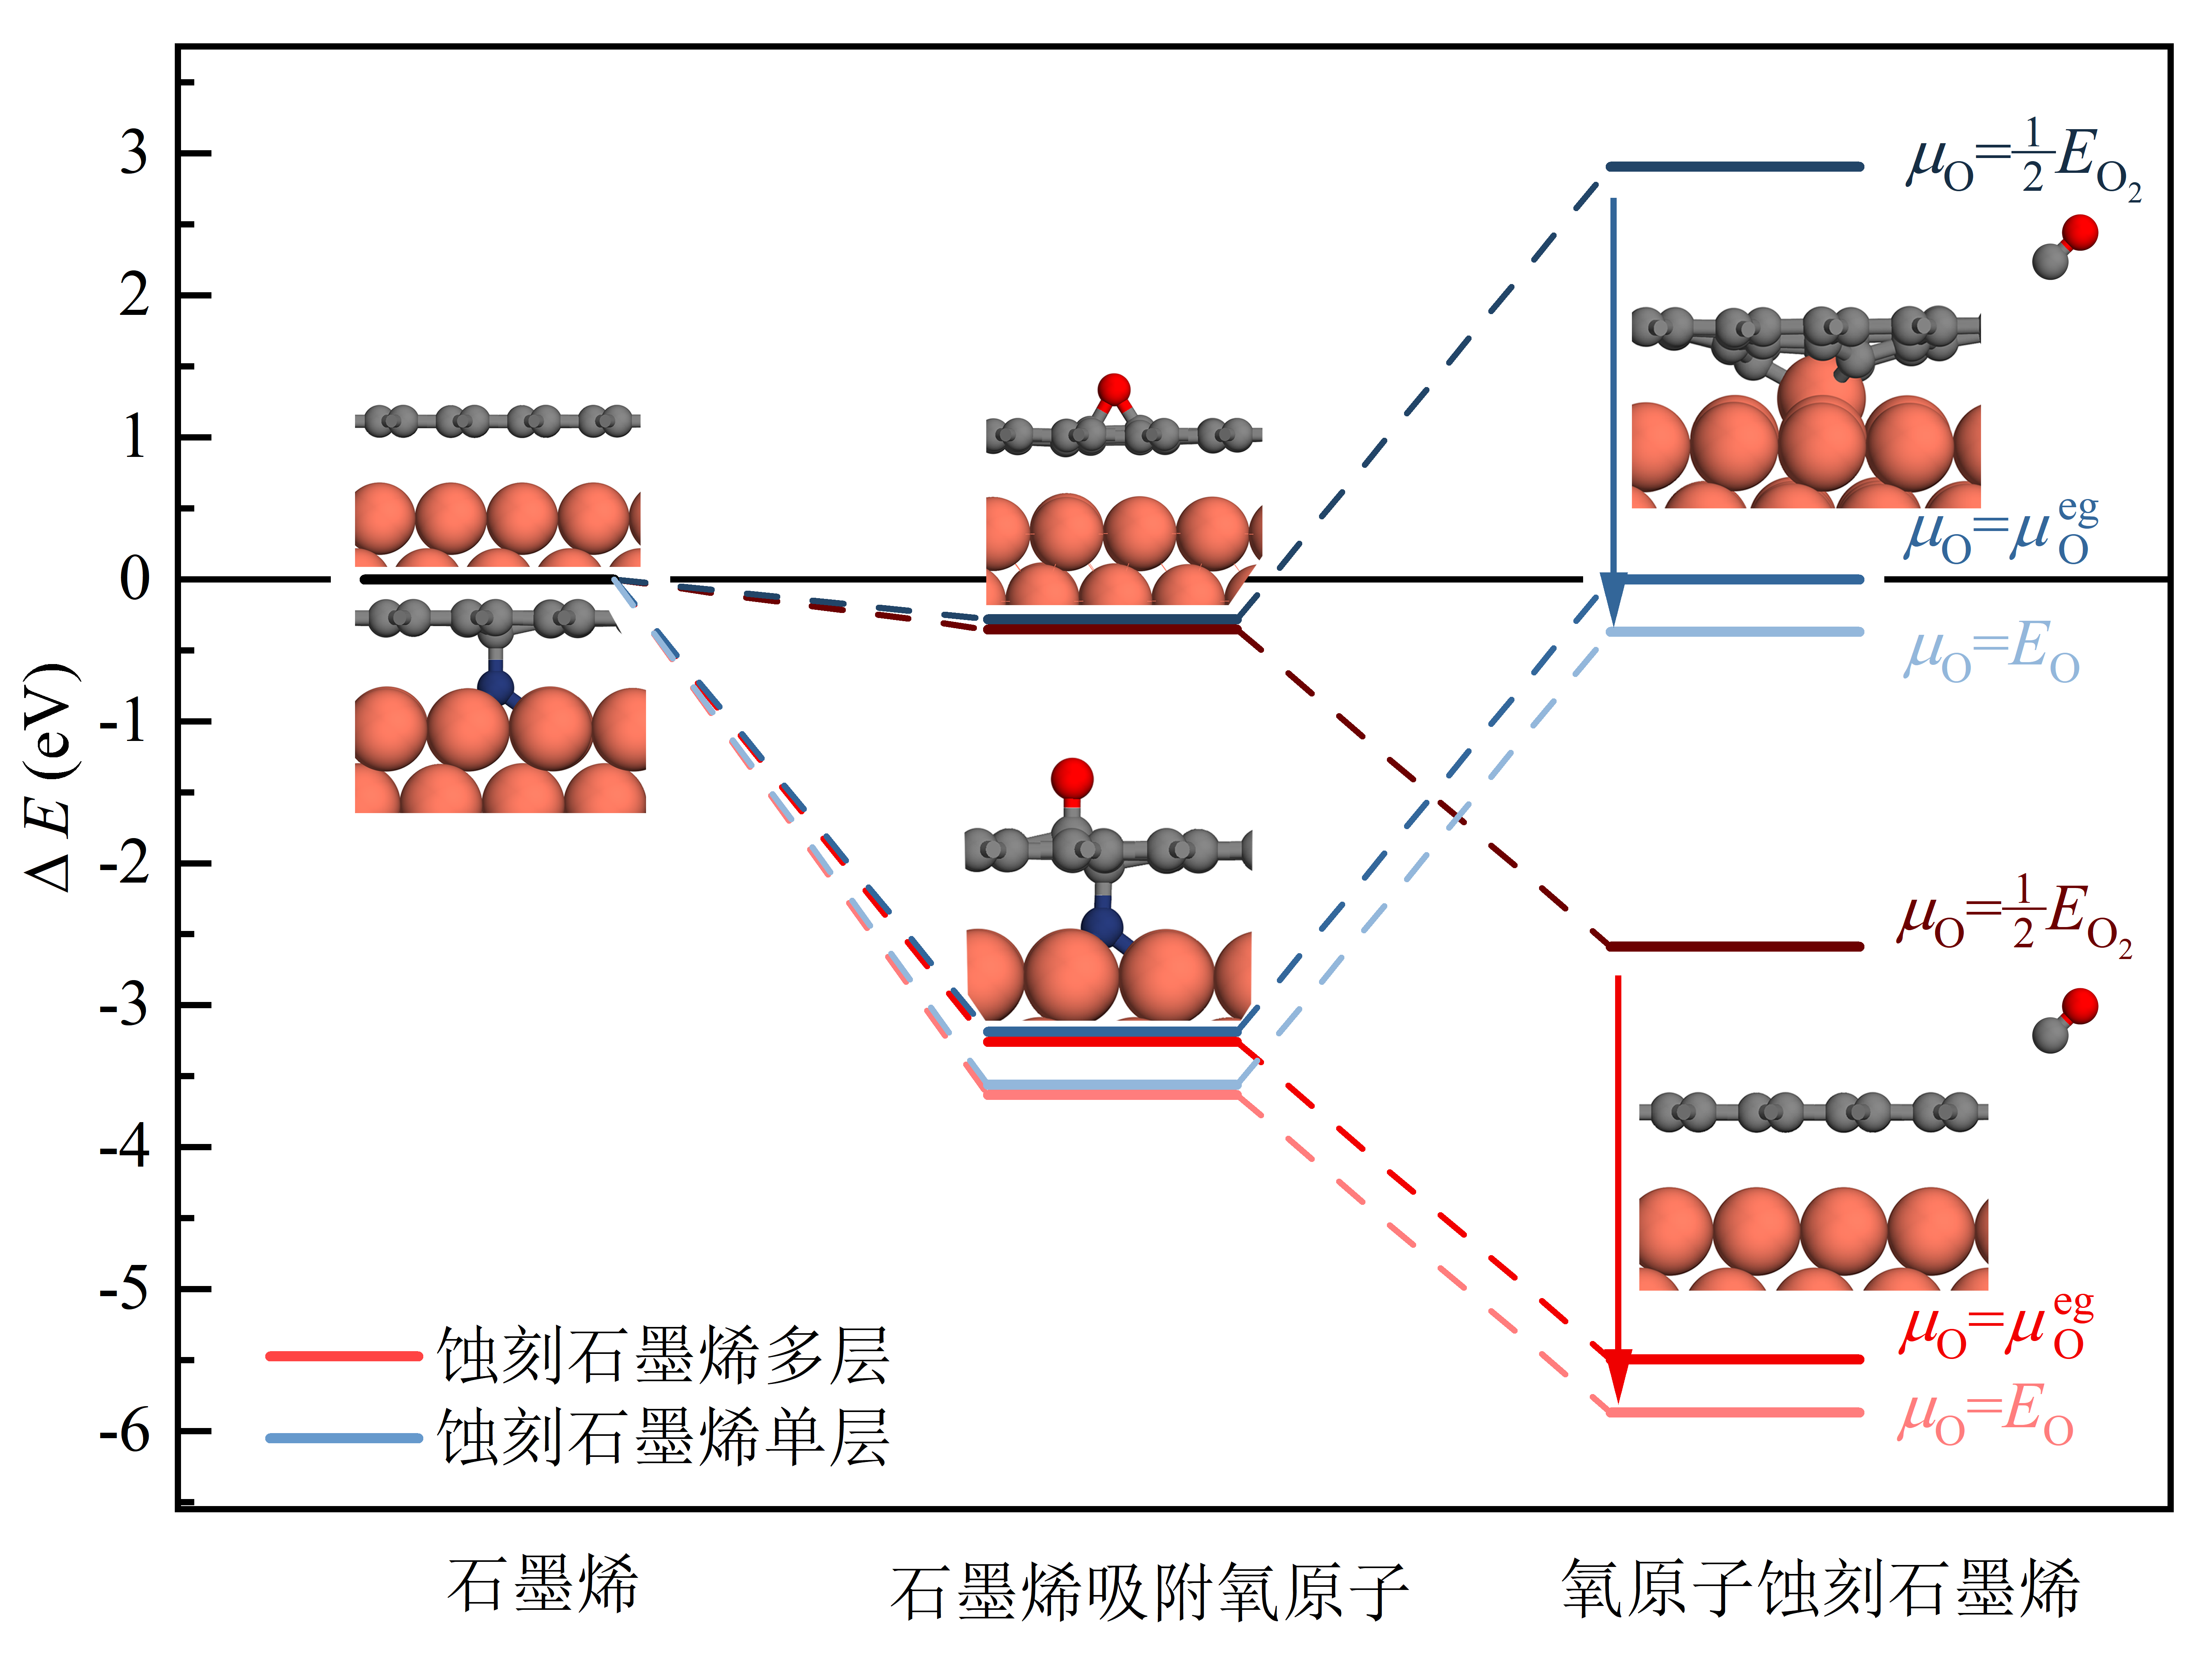
\includegraphics{pic/FLG_DFT_Oetch.png}
    \caption{石墨烯多层以及石墨烯单层在含氧环境下的蚀刻。$\muO{eg}$为氧蚀刻石墨烯单层时的平衡化学势。图中,\cemb{Cu}原子、\cemb{C}原子、氧原子、氢原子分别使用橙色、灰色、红色和白色标识。}
    \label{fig:FLG_DFT_Oetch}
\end{figure}

氧原子吸附在石墨烯上后,和石墨烯表面的\cemb{C}原子发生反应,生成非常稳定的\cemb{CO}。同时,当界面游离碳存在的时候,石墨烯上被氧原子蚀刻而成的碳空位能够被游离碳修复。这种类似于交换作用的机理使得环境中的氧原子能够通过蚀刻石墨烯单层的方式减少界面游离碳的浓度$\Cdis$,进而导致石墨烯多层点的蚀刻。计算显示,氧原子在游离碳上方的石墨烯位点蚀刻石墨烯形成\cemb{CO}的反应在所有考虑的氧原子能级$\muO{}$下都为放热反应,在$\muO{}=\halfEOm$时反应能$\rm{\Delta} \it E=\SI{-2.59}{\electronvolt}$;在$\muO{}=\EOa$时反应能$\rm{\Delta} \it E=\SI{-5.87}{\electronvolt}$。这意味着即使环境中只存在少量的氧气($\muO{} \approx \halfEOm$),生长气氛中的氧就能够通过蚀刻石墨烯单层和游离碳的交换作用对界面处的石墨烯多层进行蚀刻。

当界面处的石墨烯多层被完全蚀刻、游离碳的浓度$\Cdis$也被环境中的氧消耗至零时,氧气与石墨烯单层表面\cemb{C}原子反应产生的碳空位无法被修复,在石墨烯表面产生高能态的单空位缺陷(Single vacancy, SV)。空位缺陷的产生会极高地抬升氧原子蚀刻石墨烯单层的反应能。导致的结果是只有当环境中氧原子的能级水平提高至接近\cemb{O}自由基的能级$\EOa$时,蚀刻反应才能够从吸热反应变为放热反应,此时的$\muO{} \leqslant  \muO{eg}  $,才能够进一步对石墨烯单层进行蚀刻。$\muO{eg}$为氧蚀刻石墨烯单层时的平衡化学势。因此,对于石墨烯单层的蚀刻需要通入更高流量的氧气以抬高生长气氛中氧的反应活性。

\subsection{氧辅助石墨烯多层点的穿透生长作用}
\label{subsec:Opene}
在第\ref{subsec:FLG_gasPhase}节中,利用气相反应动力学的方法模拟了在引入不同流量的氧气的情况下石墨烯生长位点的气相化合物的浓度分布情况。对于生长物质,气相反应动力学计算发现\cemb{C2H2}分子的摩尔浓度相比于其他的生长物质的浓度高出多个数量级。因此考虑将\cemb{C2H2}分子作为本章的主要研究对象,探究其对于石墨烯多层生长的影响。

本节的研究首先通过密度泛函理论计算考察\cemb{C2H2}在石墨烯表面的吸附机理(图\ref{fig:FLG_DFT_C2H2toCHO})。对于无氧生长气氛下的石墨烯,计算结果显示\cemb{C2H2}在其上的吸附反应是吸热的,吸附能为$\SI{0.11}{\electronvolt}$。
这一结果和已有的研究吻合\citing{RN248-2014}。吸热的吸附过程说明\cemb{C2H2}较难在纯石墨烯上吸附,因此也较难对石墨烯多层点的生长产生作用。

在有氧的生长气氛下,第\ref{subsec:FLG_Oetch}节中已经证明了生长气氛中的氧在能量上很容易在石墨烯的表面形成吸附氧原子。当石墨烯的表面存在吸附氧原子时,进一步的计算显示气氛中的\cemb{C2H2}可以与吸附氧原子反应,在石墨烯的表面形成\cemb{C2H2O}。这一步骤的反应能下降为$\SI{-1.54}{\electronvolt}$。随后,石墨烯表面吸附的\cemb{C2H2O}能够进一步和氧反应,形成更为稳定的\cemb{C2H2O2}。\cemb{C2H2O2}在石墨烯的表面可以分解成为两个分离的\cemb{CHO},进一步降低体系能量。在反应过程中,仅有\cemb{C2H2O2}分解为石墨烯表面相邻的\cemb{CHO}(图\ref{fig:FLG_DFT_C2H2toCHO},G-2HCO)过程中有小至$\SI{0.027}{\electronvolt}$的反应能上升,其余过程均为放热反应。因此可以在生长气氛中引入氧气的情况下,气氛中的\cemb{C2H2}可以大量的在石墨烯的表面吸附,随后分解成为同样吸附在石墨烯表面的\cemb{CHO}。

\begin{figure}[htb]
    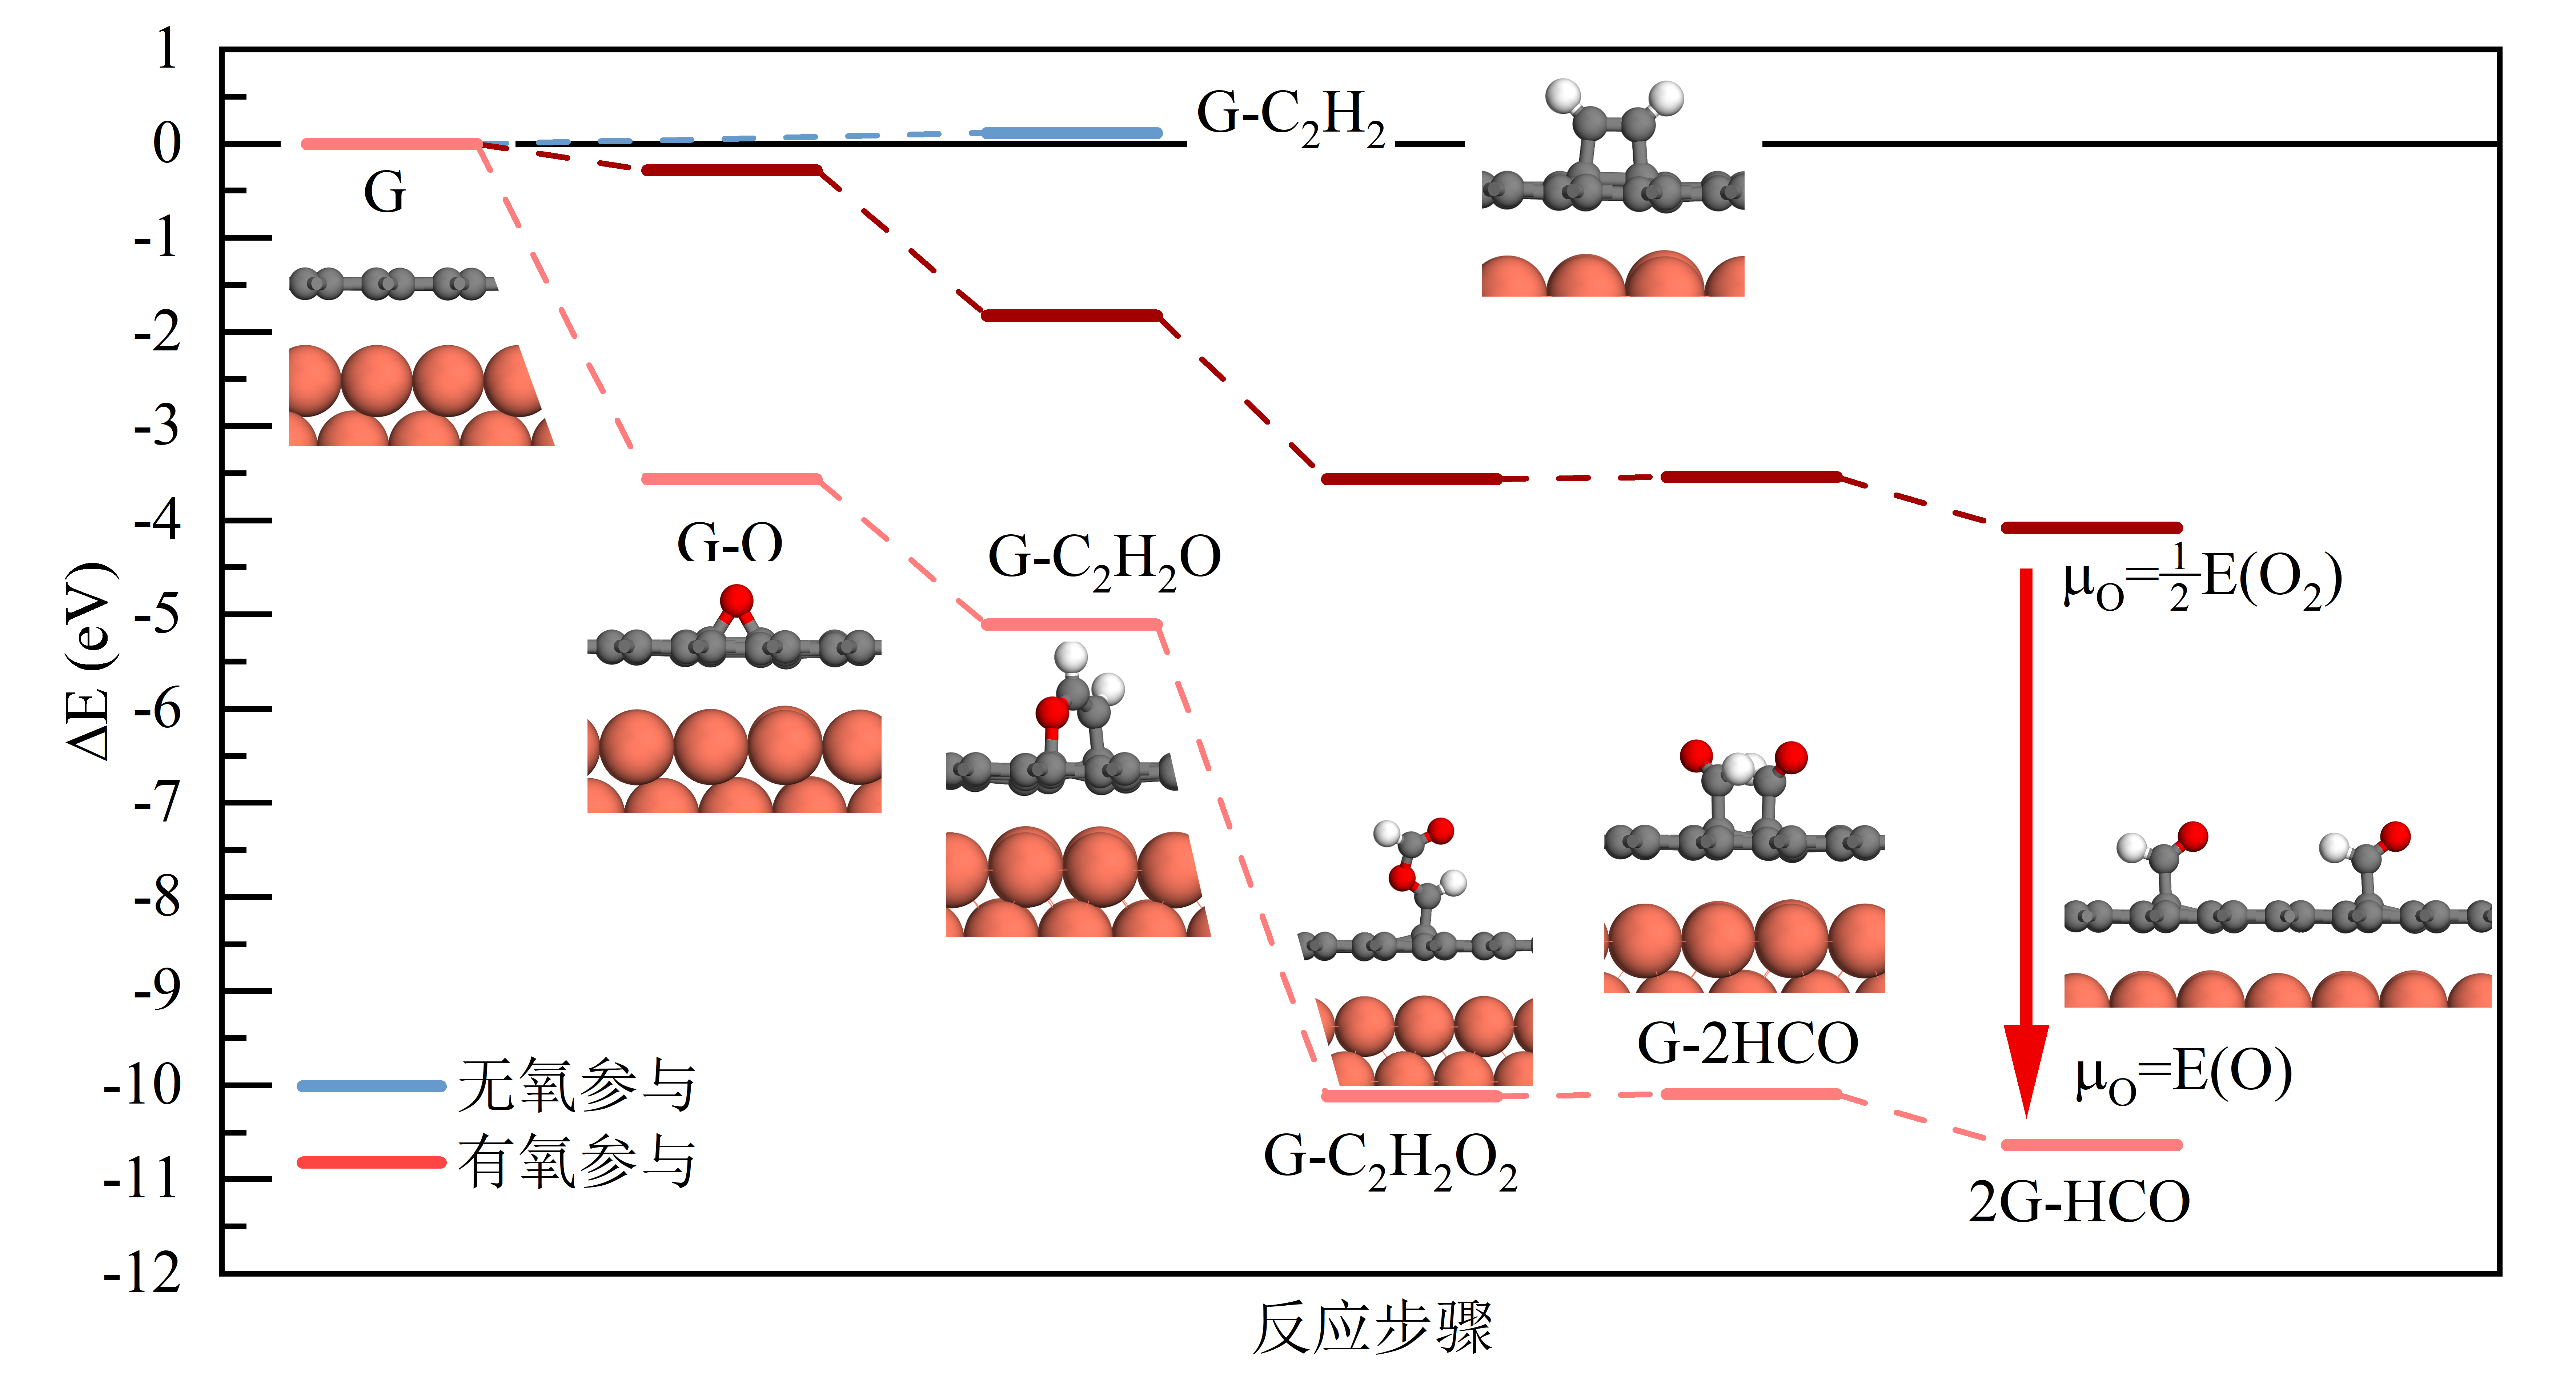
\includegraphics{pic/FLG_DFT_C2H2toCHO.png}
    \caption{氧辅助\cemb{C2H2}在石墨烯表面沉积、分解为\cemb{CHO}。图中,\cemb{Cu}原子、\cemb{C}原子、氧原子、氢原子分别使用橙色、灰色、红色和白色标识}
    \label{fig:FLG_DFT_C2H2toCHO}
\end{figure}

先前的研究表明,碳自由基以及碳氢化合物(\cemb{CH_x})等物质能够通过穿透的方式,在已生长的石墨烯的下方生长石墨烯多层\citing{RN248-2014}。考虑到碳自由基在生长气氛中极低的浓度比例,以及生长环境中较高的氢自由基浓度,在本节的研究中选择\cemb{CH}作为代表化合物考察碳自由基以及碳氢化合物在含氧的生长气氛下对于石墨烯的穿透生长作用。图\ref{fig:FLG_DFT_CHpene}中展示了计算获得的石墨烯表面吸附的\cemb{CH}在有氧和无氧的气氛下可能的穿透反应路线。计算结果显示在无氧的气氛下,\cemb{CH}能够很好得在石墨烯得表面吸附并且通过穿透作用形成界面游离\cemb{C}原子($\rm G-C_{inter}-H$)。

\begin{figure}[htb]
    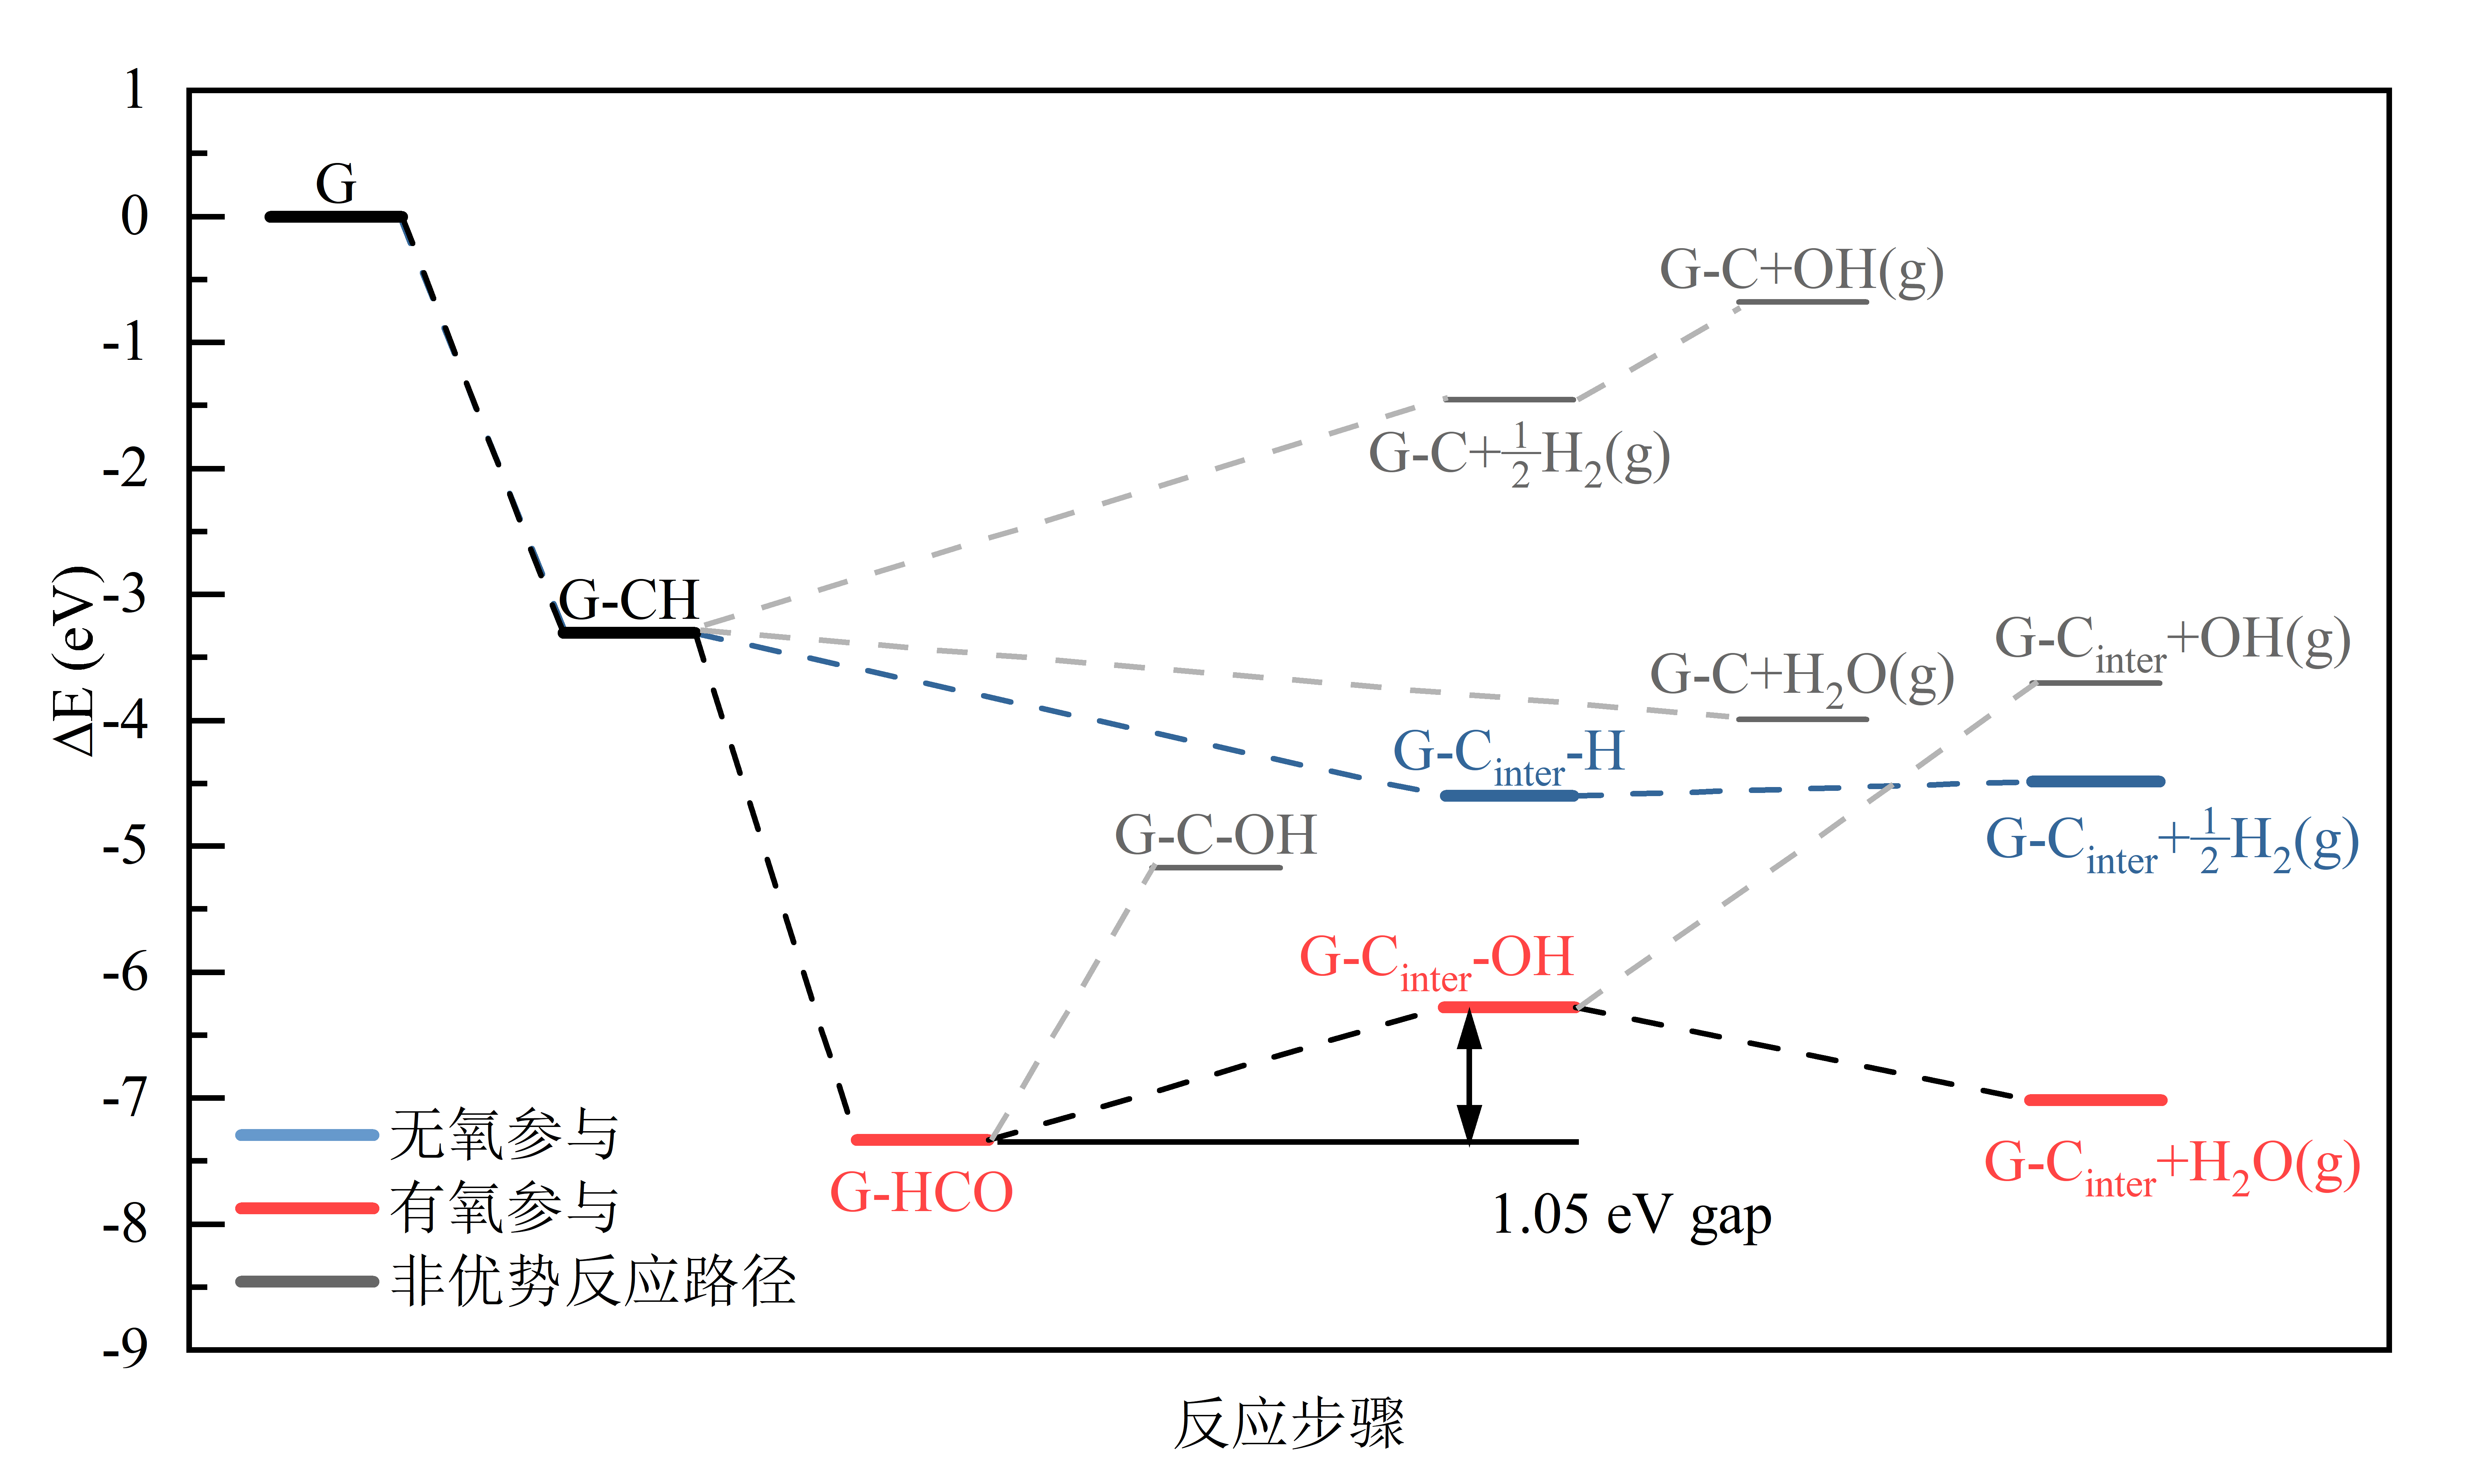
\includegraphics{pic/FLG_DFT_CHpene.png}
    \caption{含氧气氛下石墨烯表面\cemb{CH}的穿透反应过程}
    \label{fig:FLG_DFT_CHpene}
\end{figure}

然而在有氧的情况下,在石墨烯表面吸附的\cemb{CH}会优先和氧原子结合,在石墨烯的表面形成非常稳定的\cemb{CHO}。这一反应的反应能比\cemb{CH}穿透作用的反应能低$\SI{1.03}{\electronvolt}$。氧的引入阻断了\cemb{CH}通过穿透作用生长石墨烯多层的路径,并将其变为在石墨烯表面吸附的\cemb{CHO}。而\cemb{CHO}在石墨烯表面的吸附同样也遇到了困难。计算显示由于\cemb{CHO}在石墨烯表面极高的稳定性,其进行穿透反应所需吸收的能量约为$\SI{1.05}{\electronvolt}$。即使在穿透了\cemb{C}原子后,残留的\cemb{OH}官能团与气氛中的\cemb{H}反应形成水蒸气也仍旧比\cemb{CHO}在石墨烯上吸附的能量要高。

在含氧的生长气氛下,\cemb{Cu}衬底可能产生氧缺陷。而\cemb{Cu}衬底表面的氧缺陷可能会对\cemb{CHO}在石墨烯表面的穿透作用产生影响。为了简化后续计算,首先对不同构型的氧缺陷进行形成能计算和对比,筛选出合适的\cemb{Cu}衬底氧缺陷构型对后续的计算提供代表性衬底表面结构。如图\ref{fig:FLG_DFT_Odefect}所示,本节的主要考虑\cemb{Cu}衬底表面氧的三种简单的点缺陷,分别为\chinesecolon 填隙氧原子缺陷\cemb{O_{i}}、单氧原子替位缺陷\cemb{O_{Cu}}以及双氧原子替位缺陷\cemb{2O_{Cu}},其中替位缺陷均为替换单个\cemb{Cu}原子。形成能的计算使用$E_{\rm f}=E_{\rm Cu}^{\rm defect}+{\rm n_{Cu}}E_{\rm Cu}^{\rm bulk}-\frac{1}{2}{\rm n_{O}}E_{O_{2}} - E_{\rm Cu}^{\rm perfect}$。其中$E_{\rm Cu}^{\rm defect}$和$E_{\rm Cu}^{\rm perfect}$为缺陷\cemb{Cu}衬底和完美\cemb{Cu}衬底的能量;$E_{\rm Cu}^{bulk}$和$E_{O_{2}}$为块体\cemb{Cu}和氧气的能量;${\rm n_{Cu}}$和${\rm n_{O}}$为缺陷反应中涉及的\cemb{Cu}原子和氧原子的数量。计算结果显示三种点缺陷的形成能均为负值,形成能最低的单氧原子替位缺陷\cemb{O_{Cu}}的计算值为$\SI{-1.21}{\electronvolt}$。因此,可以认为在生长了石墨烯的情况下,\cemb{Cu}衬底的表面仍然很容易形成氧原子缺陷。计算得到的形成能最低的氧缺陷构型为双氧原子替位缺陷\cemb{2O_{Cu}},其形成能为$\SI{-1.94}{\electronvolt}$。在后续的计算中,使用双氧原子替位缺陷\cemb{2O_{Cu}}作为主要研究对象,考察\cemb{CHO}在石墨烯表面的穿透作用。


\begin{figure}[htb]
    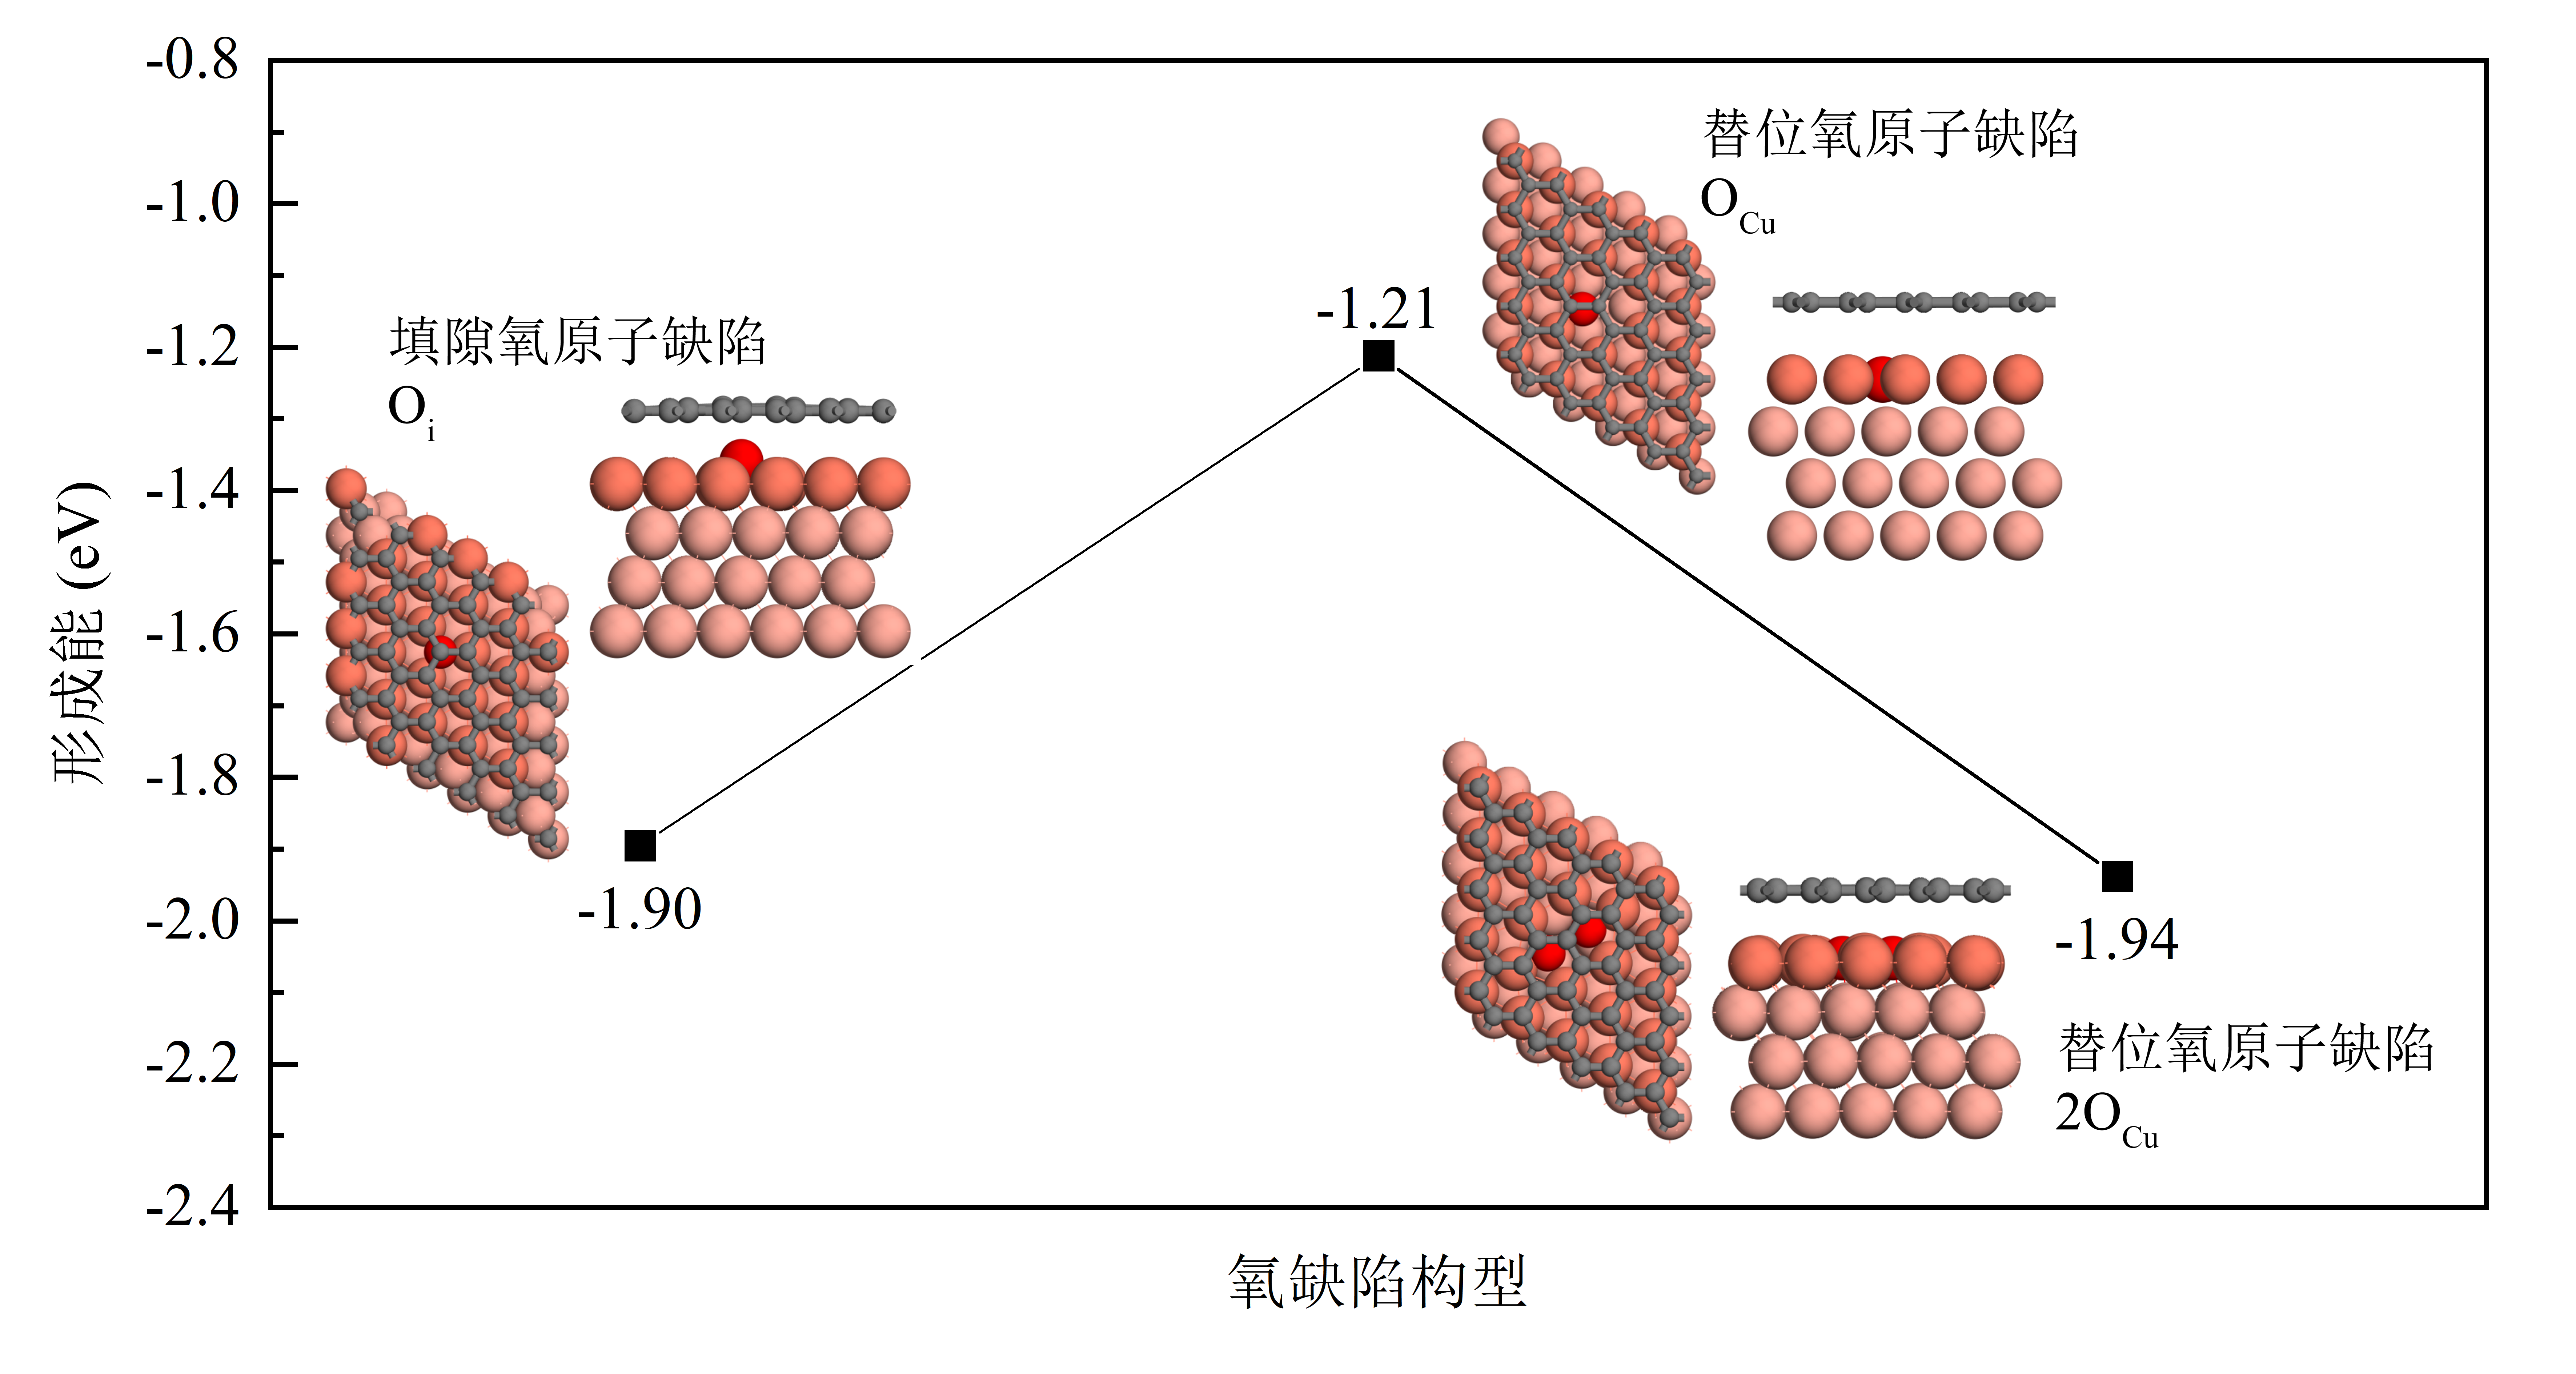
\includegraphics{pic/FLG_DFT_Odefect.png}
    \caption{\cemb{Cu}衬底表面不同构型的氧缺陷的形成能。图中,\cemb{Cu}原子、\cemb{C}原子、氧原子、氢原子分别使用橙色、灰色、红色和白色标识}
    \label{fig:FLG_DFT_Odefect}
\end{figure}

图\ref{fig:FLG_DFT_CHOpene}展示了在\cemb{Cu}衬底上不同位点的石墨烯表面吸附的\cemb{CHO}的穿透反应过程,包含无氧缺陷的原生位点以及双氧原子替位缺陷\cemb{2O_{Cu}}的氧缺陷位点。对比\cemb{CHO}在\cemb{Cu}表面原生位点的石墨烯穿透反应,\cemb{Cu}表面的氧缺陷位点对于游离碳有更高的亲和性,消除了\cemb{CHO}穿透石墨烯的上升势。


\begin{figure}[htb]
    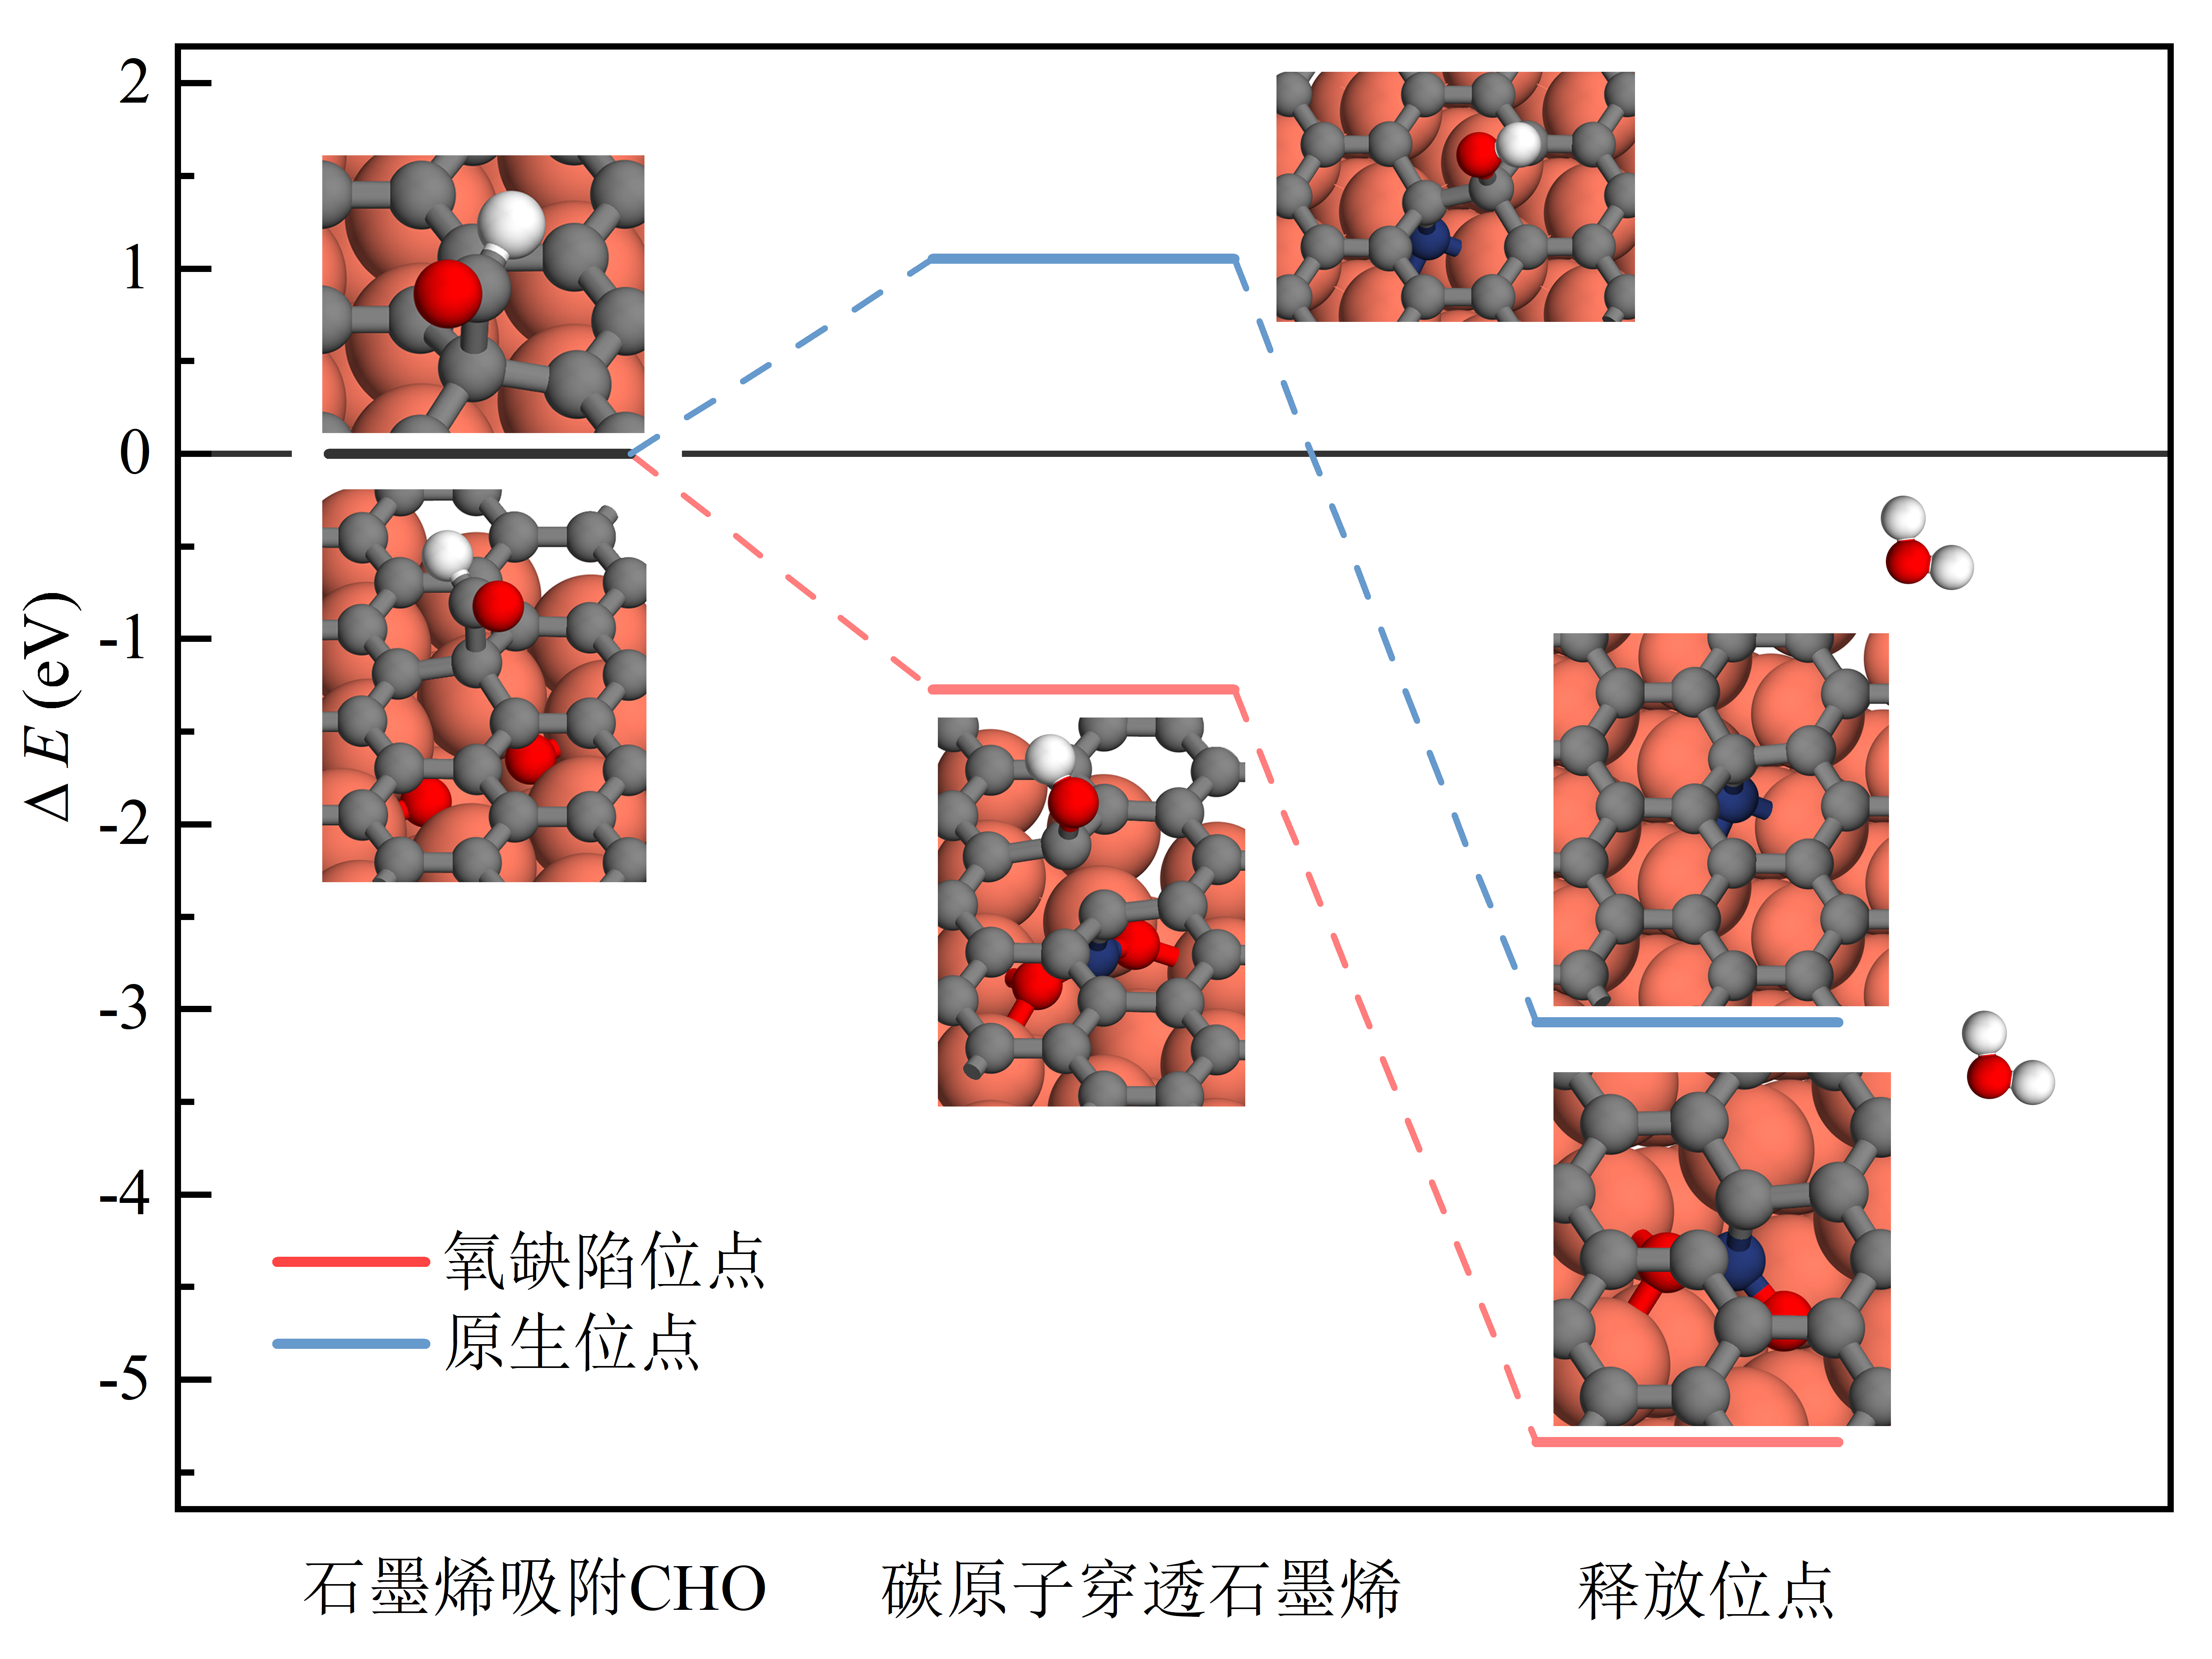
\includegraphics{pic/FLG_DFT_CHOpene.png}
    \caption{\cemb{Cu}衬底上不同位点的石墨烯表面吸附的\cemb{CHO}的穿透反应过程。图中,\cemb{Cu}原子、\cemb{C}原子、氧原子、氢原子分别使用橙色、灰色、红色和白色标识。穿透进入界面的游离\cemb{C}原子使用蓝色标识}
    \label{fig:FLG_DFT_CHOpene}
\end{figure}

在\cemb{Cu}衬底的氧缺陷位点,吸附在石墨烯表面的\cemb{CHO}的穿透反应能为$\SI{-1.27}{\electronvolt}$。同时,在穿透反应完成后,石墨烯上残留的\cemb{OH}官能团能与气氛中的氢反应,进一步降低体系能量并且释放处氧缺陷位点,使得\cemb{CHO}在氧缺陷位点的穿透反应能够持续不断的进行。虽然穿透反应过程中的交换作用使得原石墨烯单层表面的\cemb{C}原子进入界面成为游离碳,但是\cemb{CHO}对于石墨烯表面的\cemb{Cu}衬底位点选择性穿透使得在界面处生长的石墨烯多层的\cemb{C}原子主要来源于含氧气氛内的碳源。


倘若穿透反应能够在石墨烯单层表面的任意位点进行,那么由于石墨烯表面吸附分子的扩散作用,穿透进入界面的游离碳并成核生长为石墨烯多层点的\cemb{C}原子应该主要来自于原石墨烯单层的\cemb{C}原子。因为在随机作用下,只有很少的位点会产生多层点穿透的现象。如果穿透反应对于\cemb{Cu}衬底的氧缺陷位点具有选择性,氧缺陷位点处产生的穿透通道使得大部分的穿透都在氧缺陷位点上方进行,由此会产生在石墨烯单层表面多层点穿透的情况,如此一来穿透进入界面的游离碳并成核生长为石墨烯多层点的\cemb{C}原子则主要来源于生长气氛。因此,通过同位素标记法区别原石墨烯单层表面的\cemb{C}原子以及含氧气氛中的\cemb{C}原子,可以通过实验验证穿透的机制的选择性\citing{RN1262-2021}。

\subsection{氧通量调控的石墨烯多层点蚀刻/生长的模式切换模型}
综合考虑氧气的引入对于界面处石墨烯多层蚀刻和生长的影响,可以发现氧对二者均有促进作用。对于氧蚀刻反应,根据通入的氧气流量的不同导致生长气氛中氧的化学势$\muO{}$的变化,本节的研究将蚀刻反应分为两个阶段。在第一个阶段中,只有界面处的游离碳通过与石墨烯单层的交换左右,被气氛中的氧蚀刻,导致界面游离碳的浓度$\Cdis$下降,界面石墨烯多层点减少。第二个阶段是当通入的氧流量足够高时,氧的化学势超过蚀刻石墨烯单层的平衡化学势$\muO{} \geqslant \muO{eg}$,导致石墨烯单层开始被氧蚀刻。可以将氧对石墨烯的蚀刻作用总结为式\eqref{chemeq:OetchReaction}所示的化学表达式\chinesecolon
\begin{equation}
    \label{chemeq:OetchReaction}
    \begin{split}
        \ce{C($\rm dis.$) + O($\rm ads.$) &->[graphene] CO(g)} \\[+1ex]
        \ce{C(graphene) + O($\rm ads.$) + 2H &->[\hphantom{graphene}] CO(g) } \mbox{ only if $\muO{} \geqslant \muO{eg}$}
    \end{split}
\end{equation}

根据\ref{subsec:Opene}章,氧辅助的穿透反应可以写为式\eqref{chemeq:OpeneReaction}\chinesecolon
\begin{align}
    \label{chemeq:OpeneReaction}
    \cemb{C2H2(g) + 2O($\rm ads.$) + 2H(g) ->[graphene][Cu oxygen defect] 2C(adlayer) + H2O(g)}
\end{align}

根据反应式\eqref{chemeq:OetchReaction},可以写出理想状况下的蚀刻速率(式\eqref{chemeq:etchRate})\chinesecolon
\begin{equation}
    \label{chemeq:etchRate}
    \RateV{e}{}=\rule[0ex]{0ex}{8ex}\left\{
        \begin{array}{ll}
        \smash[t]{\overbrace{\RateK{e}{dis.}\Cdis\Oads}^{\mathclap{{\mbox{\normalsize $\RateV{e}{dis.}$}}}}} & \mbox{}  \\[+1ex]
        \smash[b]{\RateK{e}{dis.}\Cdis\Oads+\RateK{e}{g}\Oads} & \mbox{for $\muO{} \geqslant \muO{eq}$} 
        \end{array}\right.
        %\begin{array}{ll}\hline
        %    \rule[10ex]{1ex}{4ex}\\\hline
        %\end{array}
\end{equation}

和穿透速率(式\eqref{chemeq:peneRate})\chinesecolon
\begin{equation}
    \label{chemeq:peneRate}
    \RateV{g}{}=\RateK{g}{}\cemb{[C2H2][H2]^2}\Oads^2
\end{equation}
其中,$\RateK{e}{dis.}$、$\RateK{e}{g}$和$\RateK{g}{}$分别为游离碳蚀刻,石墨烯单层蚀刻,石墨烯多层生长的反应常数。$\Cdis$、$\cemb{[C2H2]}$、$\cemb{[H]}$和$\Oads$代表界面游离碳、$\cemb{C2H2}$化合物、$\cemb{H}$自由基以及石墨烯上吸附氧的浓度。

考虑蚀刻石墨烯多层的交换作用机理,氧原子对于的界面游离碳消耗可以用式\eqref{eq:FLG_Odis_cost}进行描述\chinesecolon
\begin{equation}
    \label{eq:FLG_Odis_cost}
    \RateV{e}{dis.}=\RateK{e}{dis.}\left(\Cdis-\RateV{e}{dis.}\right)\Oads
\end{equation}
其中,$t$为反应的时间。随着氧原子对石墨烯多层蚀刻的进行,界面游离碳逐渐被消耗,$\Cdis$的下降同时降低了石墨烯多层蚀刻反应的速率。将反应速率$\RateV{e}{dis.}$对反应时间$\ReactTime{O}{}$积分并取平均,可以得到$\ReactTime{O}{}$时间段内的氧气对游离碳的平均蚀刻反应速率如式\eqref{eq:FLG_avgEtchRate}所示\chinesecolon
\begin{equation}
    \label{eq:FLG_avgEtchRate}
    \overline{\RateV{e}{dis.}}=\frac{\int_{0}^{\ReactTime{O}{}} \RateV{e}{dis.} \,dt }{\ReactTime{O}{}}=\frac{\int_{0}^{\ReactTime{O}{}} \frac{\RateK{e}{dis.}\Cdis\Oads}{\RateK{e}{dis.}\Oads \ReactTime{}{} + 1} \,dt}{\ReactTime{O}{}}
\end{equation}

而对于生长反应,$\cemb{CHO}$在石墨烯表面的选择性吸附使得生长反应速率$\RateV{g}{}$存在一个由\cemb{Cu}衬底表面氧缺陷位点数量限制的上界。可以写出在氧缺陷处的穿透通道被饱和之前的生长反应的平均速率如式\eqref{eq:FLG_avgPeneRate}所示\chinesecolon
\begin{equation}
    \label{eq:FLG_avgPeneRate}
    \overline{\RateV{g}{}}=\frac{\int_{0}^{\ReactTime{O}{}} \RateV{g}{} \,dt }{\ReactTime{O}{}}= \frac{\int_{0}^{\ReactTime{O}{}} \RateK{g}{}\cemb{[C2H2][H2]^2}\Oads^2 \,dt }{\ReactTime{O}{}}
\end{equation}

在这些化合物的浓度中,$\cemb{[C2H2]}$和$\cemb{[H]}$的取值可以采用第\ref{subsec:FLG_gasPhase}节中模拟得出的相应的气相化合物的浓度数据。而对于$Odis$,虽然在\ref{subsec:FLG_gasPhase}章中的模拟证明生长环境中的化合物很快就达到了稳态平衡,但由于\cemb{O}自由基($\cemb{O}$)较低的浓度以及氧分子($\cemb{O2}$)在石墨烯表面较低的吸附能。氧气的吸附过程可能会需要很长的一段时间才会达到饱和。为了获得$\Oads$在石墨烯多层生长过程中随时间的变化情况,在本节的研究中使用晶格随机顺序吸附模型(lattice random sequential adsorption model )对氧气以及氧原子在石墨烯表面的吸附进行模拟。

在晶格随机顺序吸附模型中,本节的研究采用二维晶格对石墨烯进行模拟,每个晶格单元对应一个原胞大小的石墨烯。在模拟过程中,考虑生长气氛中氧气分子($\cemb{O2}$)和\cemb{O}自由基($\cemb{O}$)在石墨烯表面的沉积。根据密度泛函理论计算(表\ref{tab:FLG_RSA_coverage}),取$\cemb{O2}$和$\cemb{O}$在石墨烯表面吸附的饱和覆盖率分别为$1$和$1 / 4$。

\begin{table}
    \centering
    \caption{\cemb{O}和\cemb{O2}在石墨烯表面的吸附能力}
    \begin{tabular}{
        >{\centering}m{0.2\textwidth}
        >{\centering}m{0.3\textwidth}
        >{\centering\arraybackslash}m{0.3\textwidth}
    }
        \toprule
        覆盖率  & $\cemb{O}$的吸附能(\si{\electronvolt}) & $\cemb{O2}$的吸附能(\si{\electronvolt}) \\
        \midrule
        1       & -4.50                                    & 0.43                                      \\
        $1 / 4$ & -4.95                                    & -0.026                                    \\
        \bottomrule
    \end{tabular}
    \label{tab:FLG_RSA_coverage}
\end{table}

有别于\cemb{O}自由基($\cemb{O}$)的直接吸附,氧气分子($\cemb{O2}$)在石墨烯上的吸附的同时需要较高的能量进行进行裂解。\cemb{O2}裂解过程对于吸附情况的影响可以通过在氧气分子吸附的过程中添加$\SI{2.39}{\electronvolt}$的势垒进行描述\citing{RN838-2012}。为了将随机吸附模拟过程中的模拟时间时长与实际通入氩氧混合气的时长进行对应,\cemb{O}自由基($\cemb{O}$)和氧气分子($\cemb{O2}$)与石墨烯表面的碰撞频率可根据气体的麦克斯韦-玻尔兹曼分布计算而得,气氛中\cemb{O}自由基($\cemb{O}$)和氧气分子($\cemb{O2}$)的浓度也根据\ref{subsec:FLG_gasPhase}节中的模拟数据进行计算。

图\ref{fig:FLG_RSA_Oadsorb}中给出了通入不同流量的氩氧混合气的情况下石墨烯上吸附的氧原子浓度$\Oads$随时间的变化情况。

\begin{figure}[htb]
    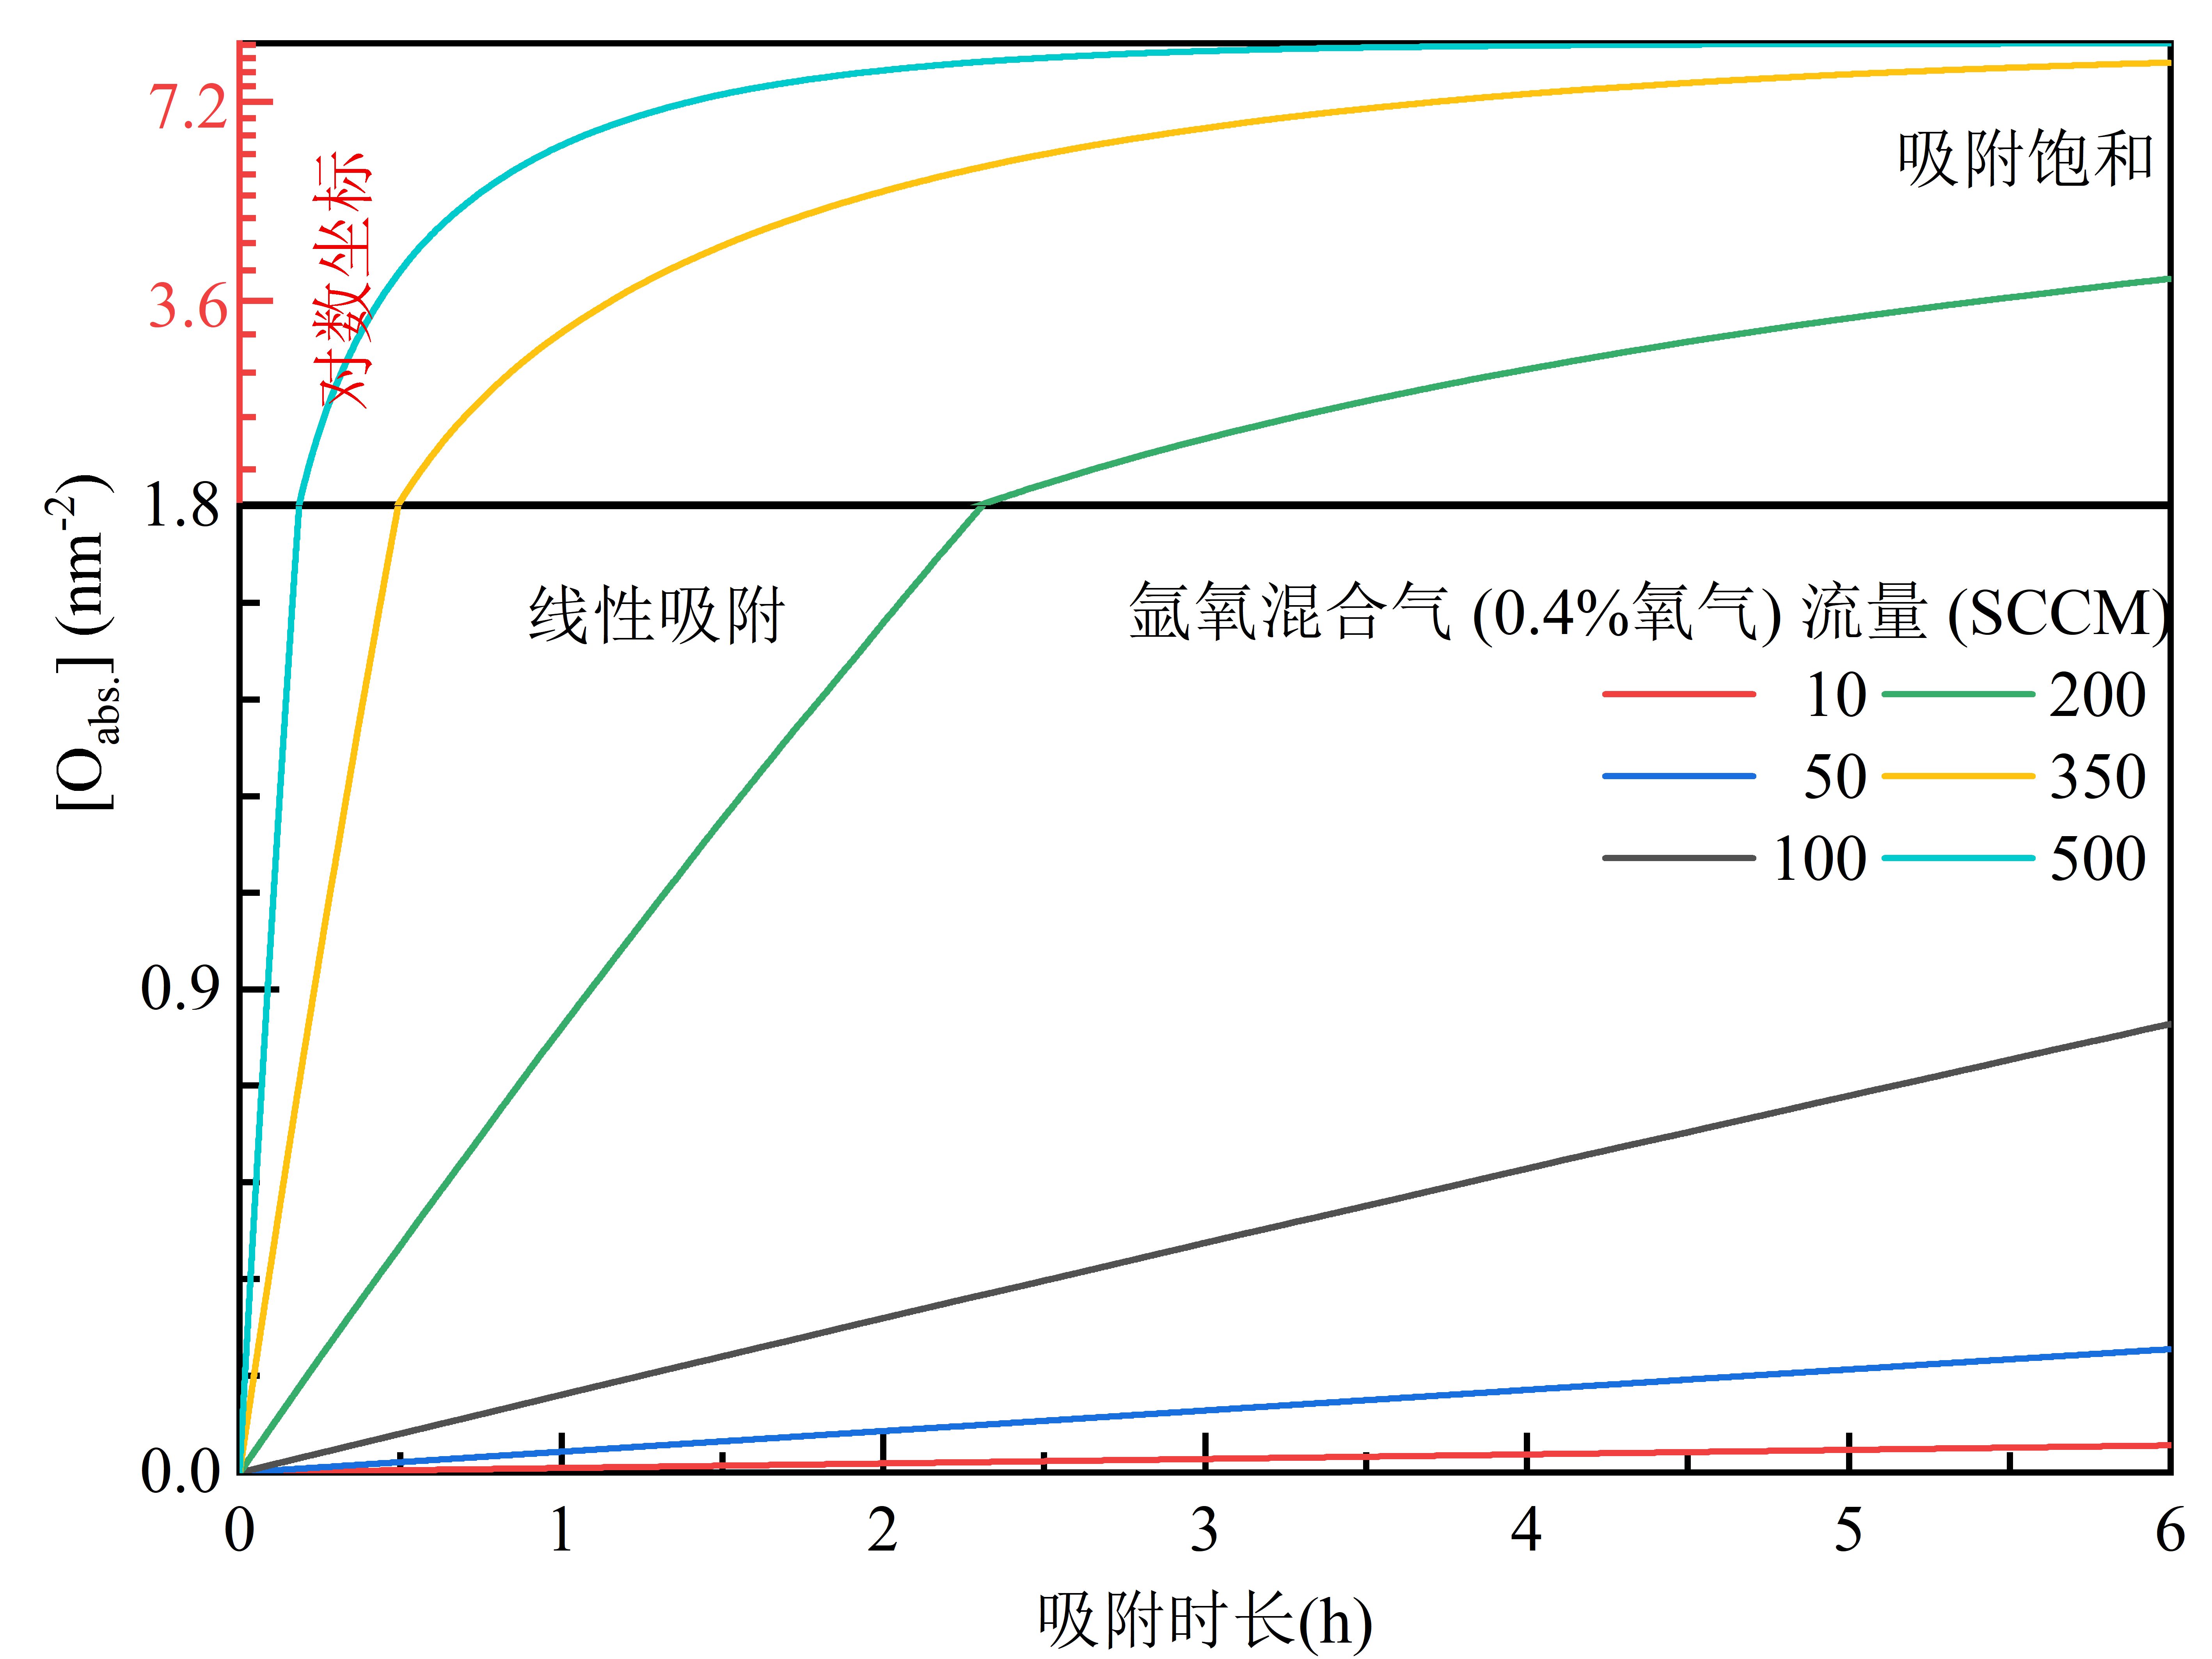
\includegraphics{pic/FLG_RSA_Oadsorb.png}
    \captionsetup{width=\textwidth}
    \caption{不同氩氧混合气通入流量下氧原子在石墨烯表面吸附浓度随时间的变化情况}
    \label{fig:FLG_RSA_Oadsorb}
\end{figure}

计算结果显示模拟得出的$\Oads$服从指数增长定律$\Oads\left(\it t\right)=\Oads\left(\it \infty \right)-\it De^{\it -\sigma t}$,和先前的研究一致\citing{RN837-1990,RN836-1991}。由于$\Oads$的指数形式,直接将$\Oads$带入计算$\overline{\RateV{e}{dis.}}$中的积分项为非初等函数。考虑到在实际的化学气相沉积生长过程中,氧原子在低浓度氧环境中需要花费数天甚至一个月的时间才能达到饱和吸附,远超普通化学气相沉积法制备石墨烯所考虑的生长时间范畴。而高浓度氧环境中会导致石墨烯被完全蚀刻,也不在本节研究所关心的范围内。因此在接下来的分析中,将研究范围集中在氧原子吸附浓度$\Oads$的线性吸附区,这时$\Oads$相对于时间的变化关系可以简化为$\Oads\left(\it t\right)\approx \it D \sigma t$。

为了确认$\Oads$线性简化是否会因为晶格随机顺序吸附模拟过程中所使用的屏蔽系数参数的变动而失效。图\ref{fig:FLG_RSA_OabsorbPera}给出了在中等氧通量的情况下(氩氧混合气流量为\SI{100}{SCCM}),多种模拟参数组合下氧原子在石墨烯表面进行吸附模拟的结果。氧气$\cemb{O2}$屏蔽系数的变化几乎无法传到至最后吸附浓度的变化。这可能是由于氧气较高的解离势垒导致尽管生长气氛中的氧气浓度较高,但氧气在石墨烯表面解离吸附在石墨烯上的能力仍然较弱。而对于\cemb{O}自由基$\cemb{O}$,屏蔽系数由$1$变为$\frac{1}{2}$会降低吸附氧原子的浓度。但考虑到通常化学气相沉积法对石墨烯的生长过程通常在$\SI{10}{\hour}$以内\citing{RN1262-2021}。在这个时间范围之内,\cemb{O}自由基$\cemb{O}$屏蔽系数的变化对吸附氧原子浓度的影响较小。同时也并不会影响吸附氧原子浓度在$\SI{10}{\hour}$之内随时间的线性增长关系。因此,可以认为对氧原子吸附浓度$\Oads$使用$\Oads\left(\it t\right)\approx \it D \sigma t$进行简化并不会受模拟过程中屏蔽系数参数选取的影响。

\begin{figure}[htb]
    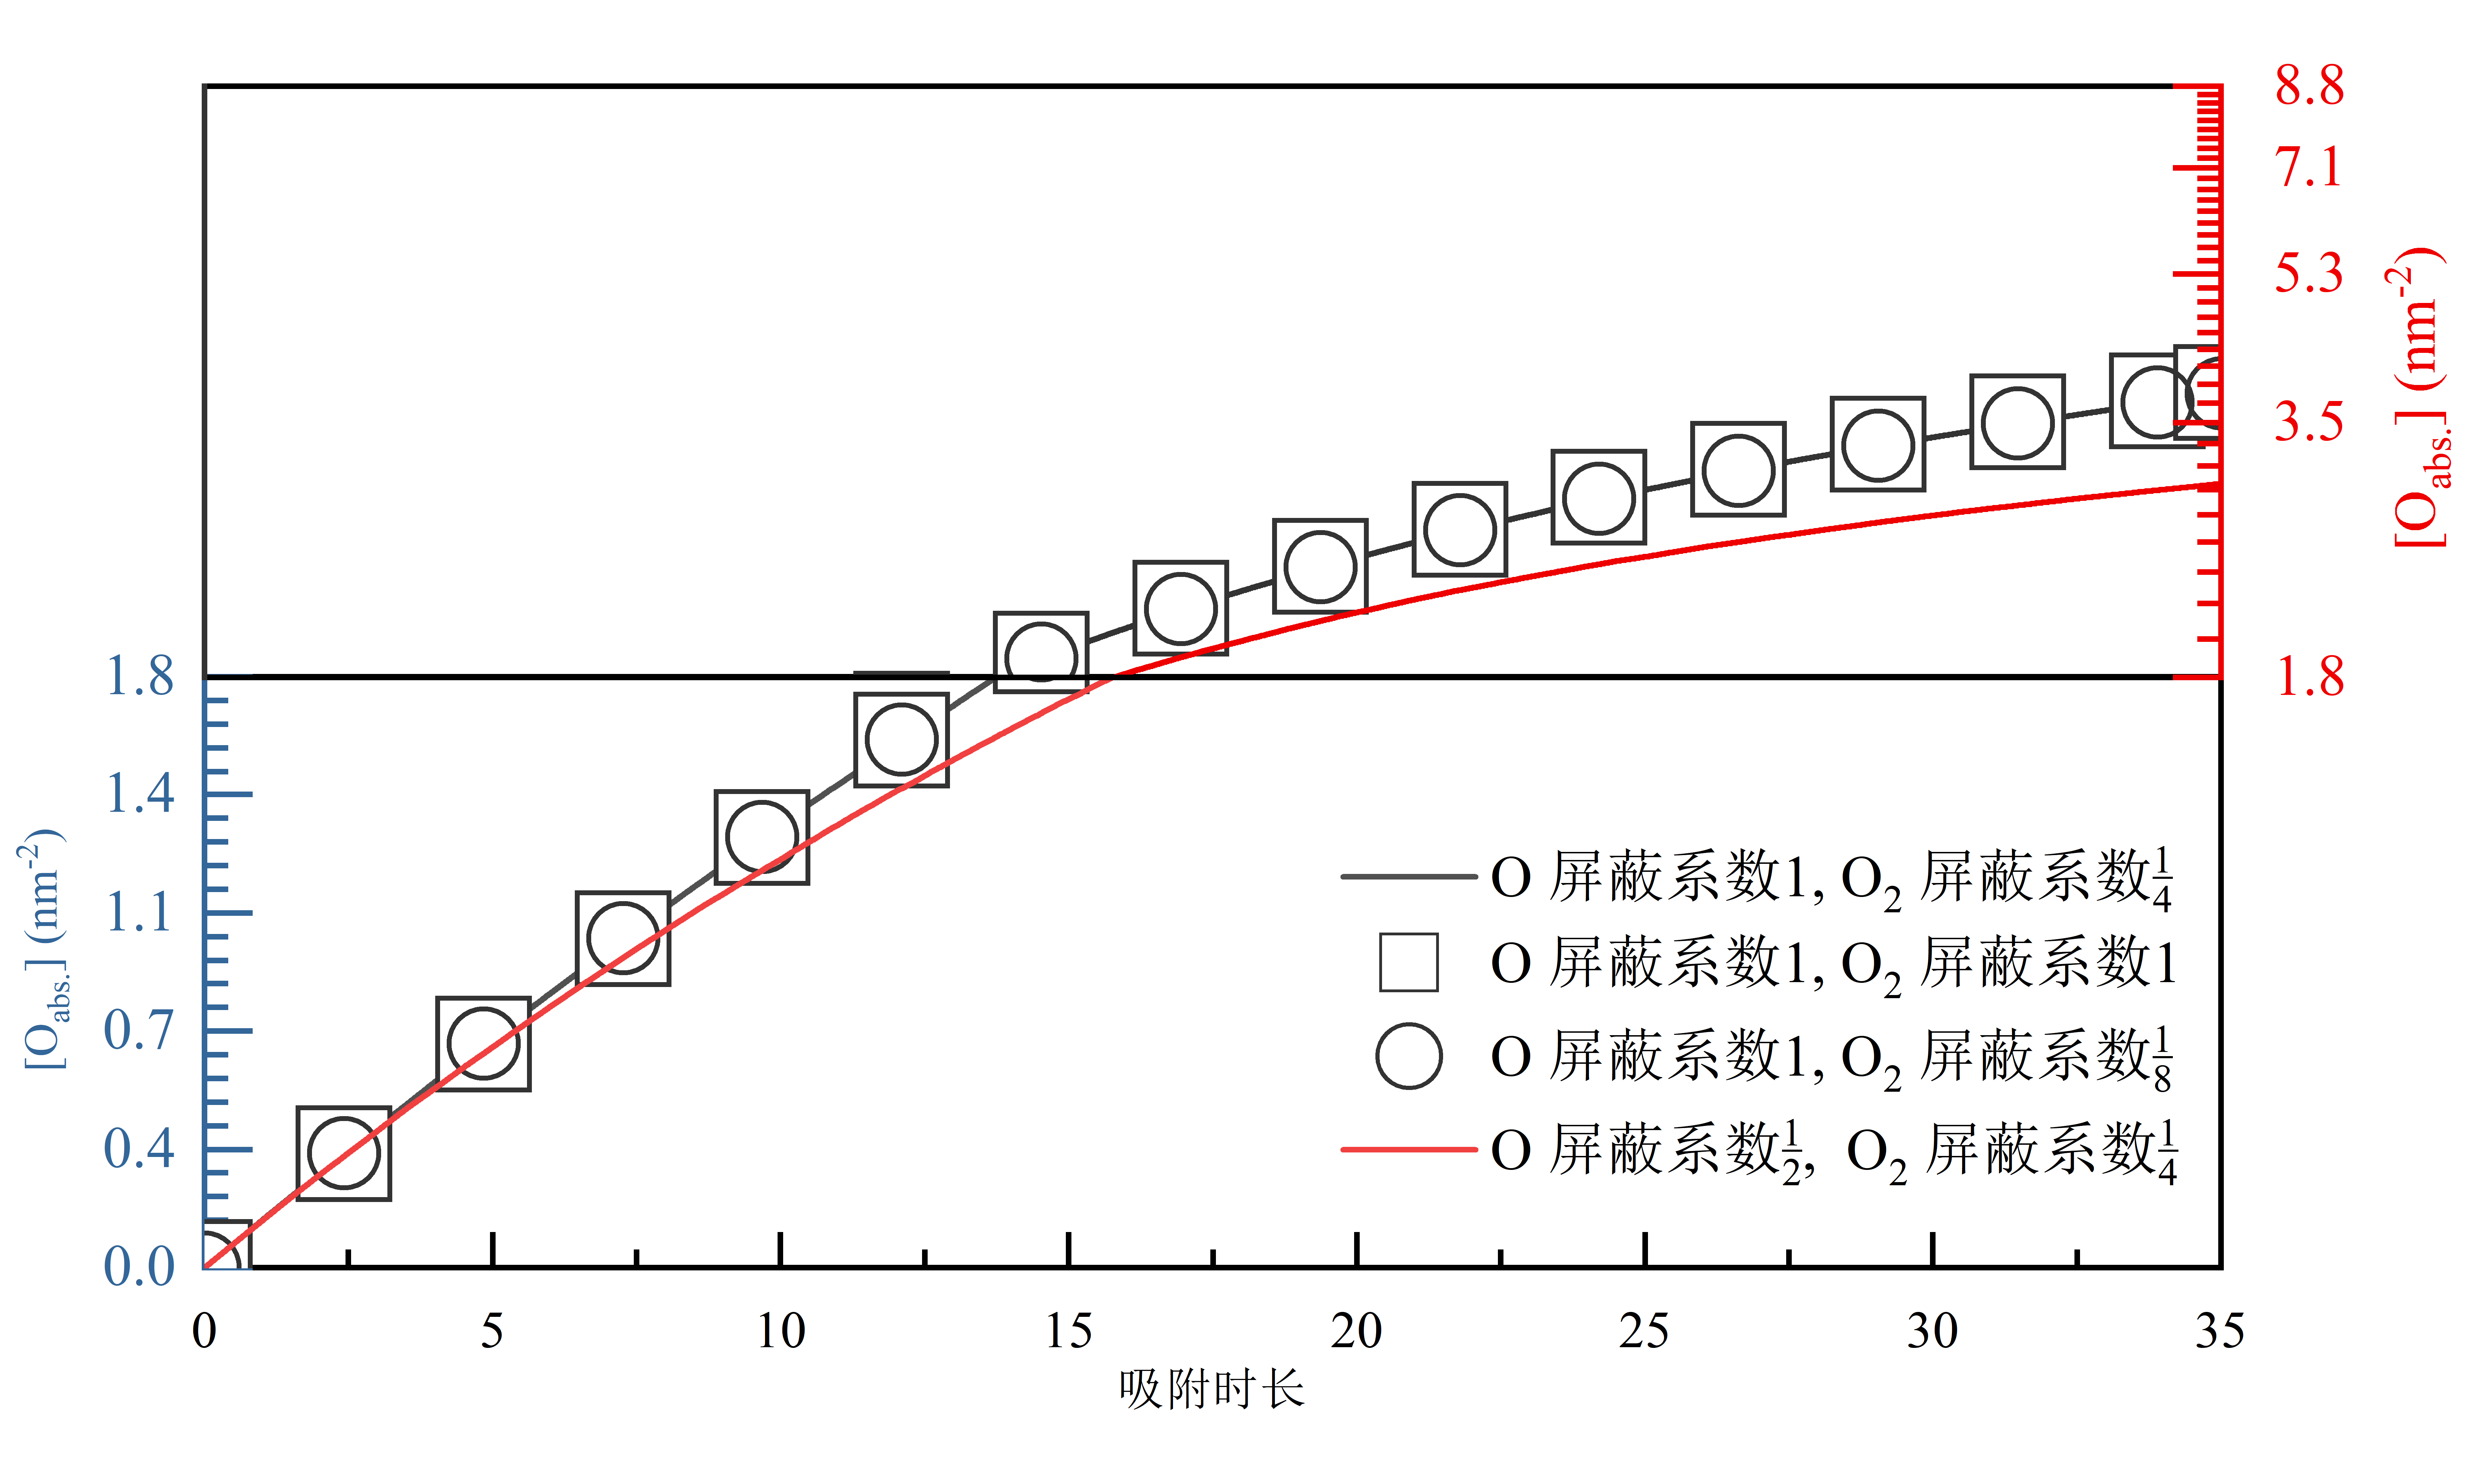
\includegraphics{pic/FLG_RSA_OabsorbPera.png}
    \caption{$\Oads\left(\it t\right)\approx \it D \sigma t$线性近似的晶格随机顺序吸附模拟参数稳定性测试}
    \label{fig:FLG_RSA_OabsorbPera}
\end{figure}

由此,可以计算通入$\ReactTime{O}{}$的氩氧混合气后,石墨烯的蚀刻平均速率为式\eqref{eq:FLG_avgVe}\chinesecolon
\begin{equation}
    \label{eq:FLG_avgVe}
    \overline{\RateV{e}{}}=
    \begin{cases}
        \frac{\Cdis_0 \log\left( 1+\RateK{e}{dis.}\Oads | \,_{t=\ReactTime{O}{}} \ReactTime{O}{} \right) }{\it 2 \ReactTime{O}{}}                                                        & \muO{} <  \muO{eg}         \\[+1ex]
        \frac{\Cdis_0 \log\left( 1+\RateK{e}{dis.}\Oads | \,_{t=\ReactTime{O}{}} \ReactTime{O}{} \right) }{\it 2 \ReactTime{O}{}} + \frac{1}{2}\RateK{e}{g}\Oads| \,_{t=\ReactTime{O}{}} & \muO{} \geqslant \muO{eg}
    \end{cases}
\end{equation}
其中,界面游离碳的初始浓度$\Cdis_0$取相应生长温度下碳的饱和蒸汽进行近似。$\Oads| \,_{t=\ReactTime{O}{}}$为氩氧混合气的时间为$\ReactTime{O}{}$时的石墨烯上的吸附氧原子浓度。

同样,也可以求得在\cemb{Cu}衬底氧缺陷产生的穿透通道饱和前,石墨烯的生长平均速率为式\eqref{eq:FLG_avgVg}\chinesecolon
\begin{equation}
    \label{eq:FLG_avgVg}
    \overline{\RateV{g}{}} =\frac{1}{3}\RateK{g}{}\cemb{[C2H2]}\cemb{[H]^2}\left(\Oads |_{\,\ReactTime{}{}=\ReactTime{O}{}} \right)
\end{equation}

式\eqref{eq:FLG_avgVe}和式\eqref{eq:FLG_avgVg}可以解释氧促石墨烯多层蚀刻和氧促石墨烯生长之间的反应速率的竞争对于石墨烯多层整体蚀刻和生长行为的影响。图\ref{fig:FLG_model_avgV}给出了不同吸附氧原子浓度下,氧辅助石墨烯蚀刻和生长作用的平均反应速率。图\ref{fig:FLG_model_avgV}中的原点代表无氧气输入的情况,此时的石墨烯呈现出自限制的生长行为。当氧气引入生长气氛时,石墨烯表面吸附的氧原子浓度$\Oads$随着氧气通入量或者含氧气氛内反应时间的上升而上升。当吸附氧原子浓度$\Oads$较低时,石墨烯多层的蚀刻速率高于石墨烯多层的生长速率,石墨烯自限制生长下的少量多层点在氧原子的蚀刻作用下逐渐减少,整体表现出石墨烯多层蚀刻的行为(模式I)。当石墨烯表面吸附氧原子的浓度$\Oads$逐渐上升时,氧原子对于石墨烯表面的蚀刻反应速率由于界面游离碳浓度$\Cdis$的下降而放缓,$\cemb{CHO}$的穿透生长反应则随着$\Oads$的上升而继续加速。此时上升的$\Oads$导致石墨烯多层的生长速率高于被界面游离碳浓度不足所限制的石墨烯多层蚀刻速率,整体展现出石墨烯多层生长的行为(模式II)。当$\Oads$的浓度上升至氧的化学势$\muO{}$超过蚀刻石墨烯单层的平衡化学势$\muO{eg}$,气氛中的氧开始直接蚀刻单层石墨烯,导致石墨烯蚀刻反应的速率大幅上升,再次超过被穿透通道饱和所限制的石墨烯多层生长速率。此时石墨烯展现出再蚀刻的行为(模式III)。在模式III中,由于较高的氧活性,不仅石墨烯多层,较为稳定的石墨烯单层也会被高反应活性的氧反应。

与实验研究者合作,通过在石墨烯生长环境中通入少量氧气的方式,成功实现了石墨烯多层点随着氧气通入量上升而出现先蚀刻,后生长,最后完全蚀刻的生长模式\citing{RN1262-2021}。与本小节中所述的氧通量调控的石墨烯多层模式切换模型吻合。

\begin{figure}[tb]
    \subfloat[]{
        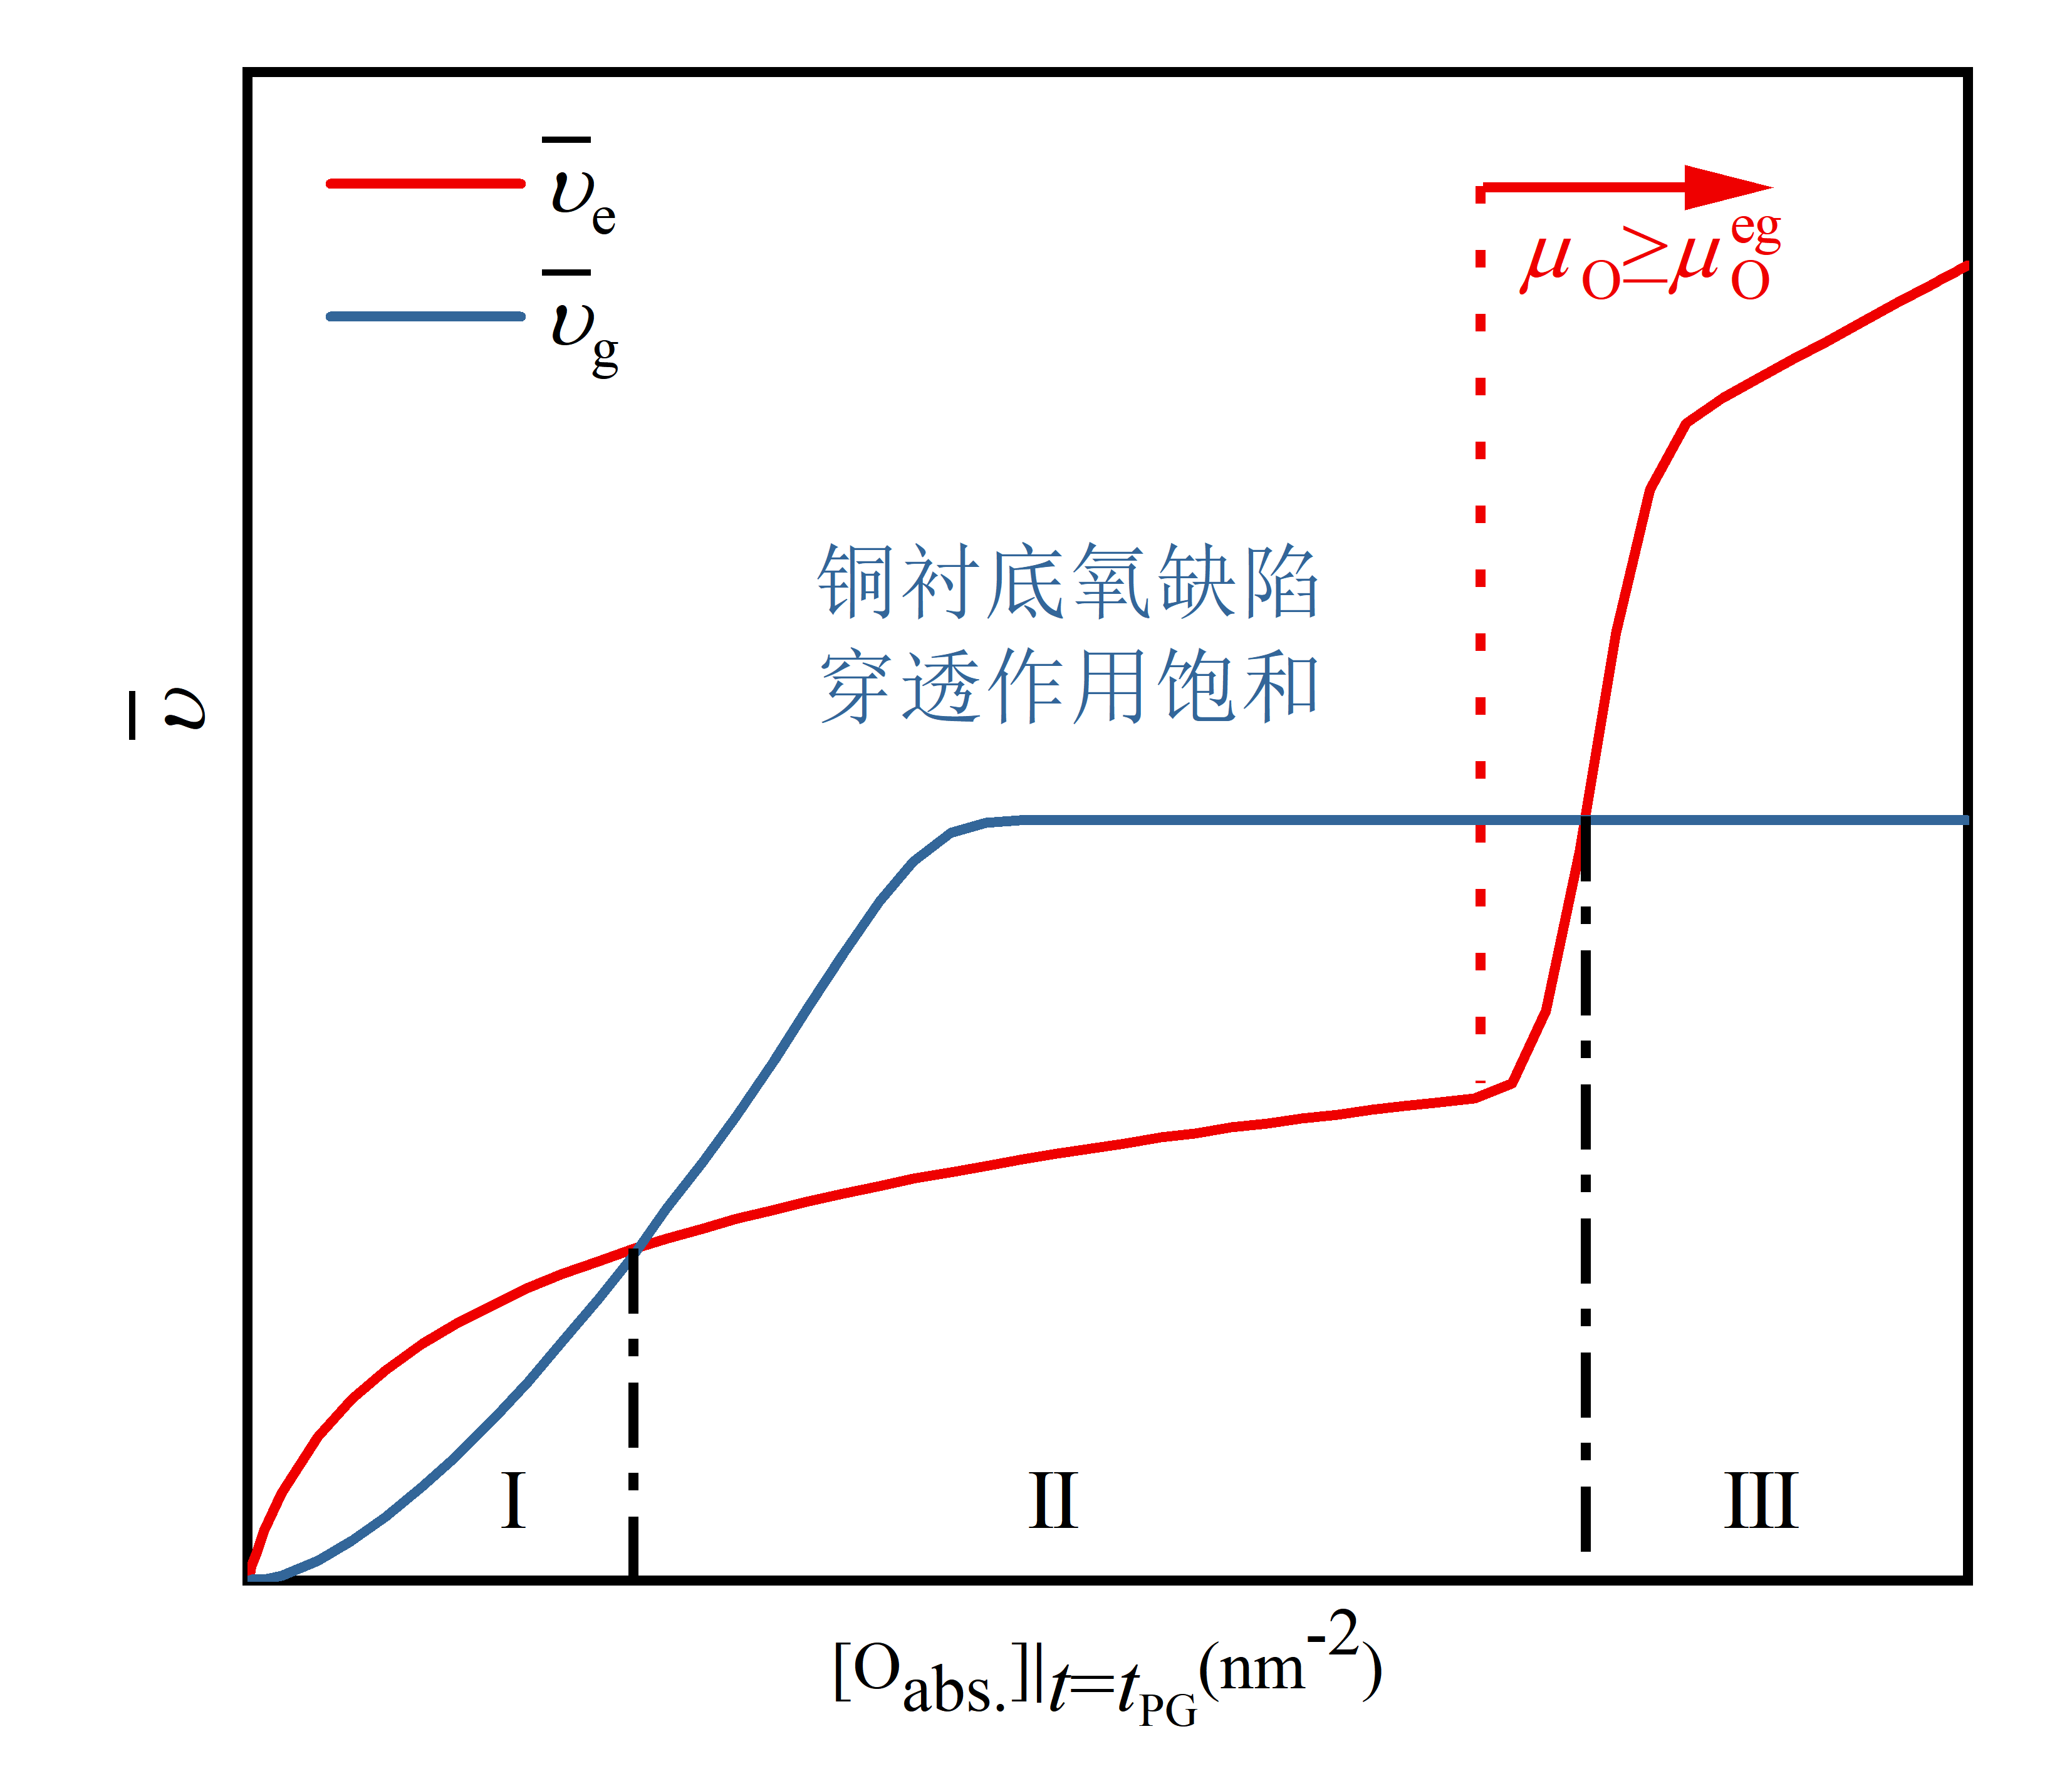
\includegraphics[]{pic/FLG_model_avgV.png}
        \label{fig:FLG_model_avgV}
    }
    \subfloat[]{
        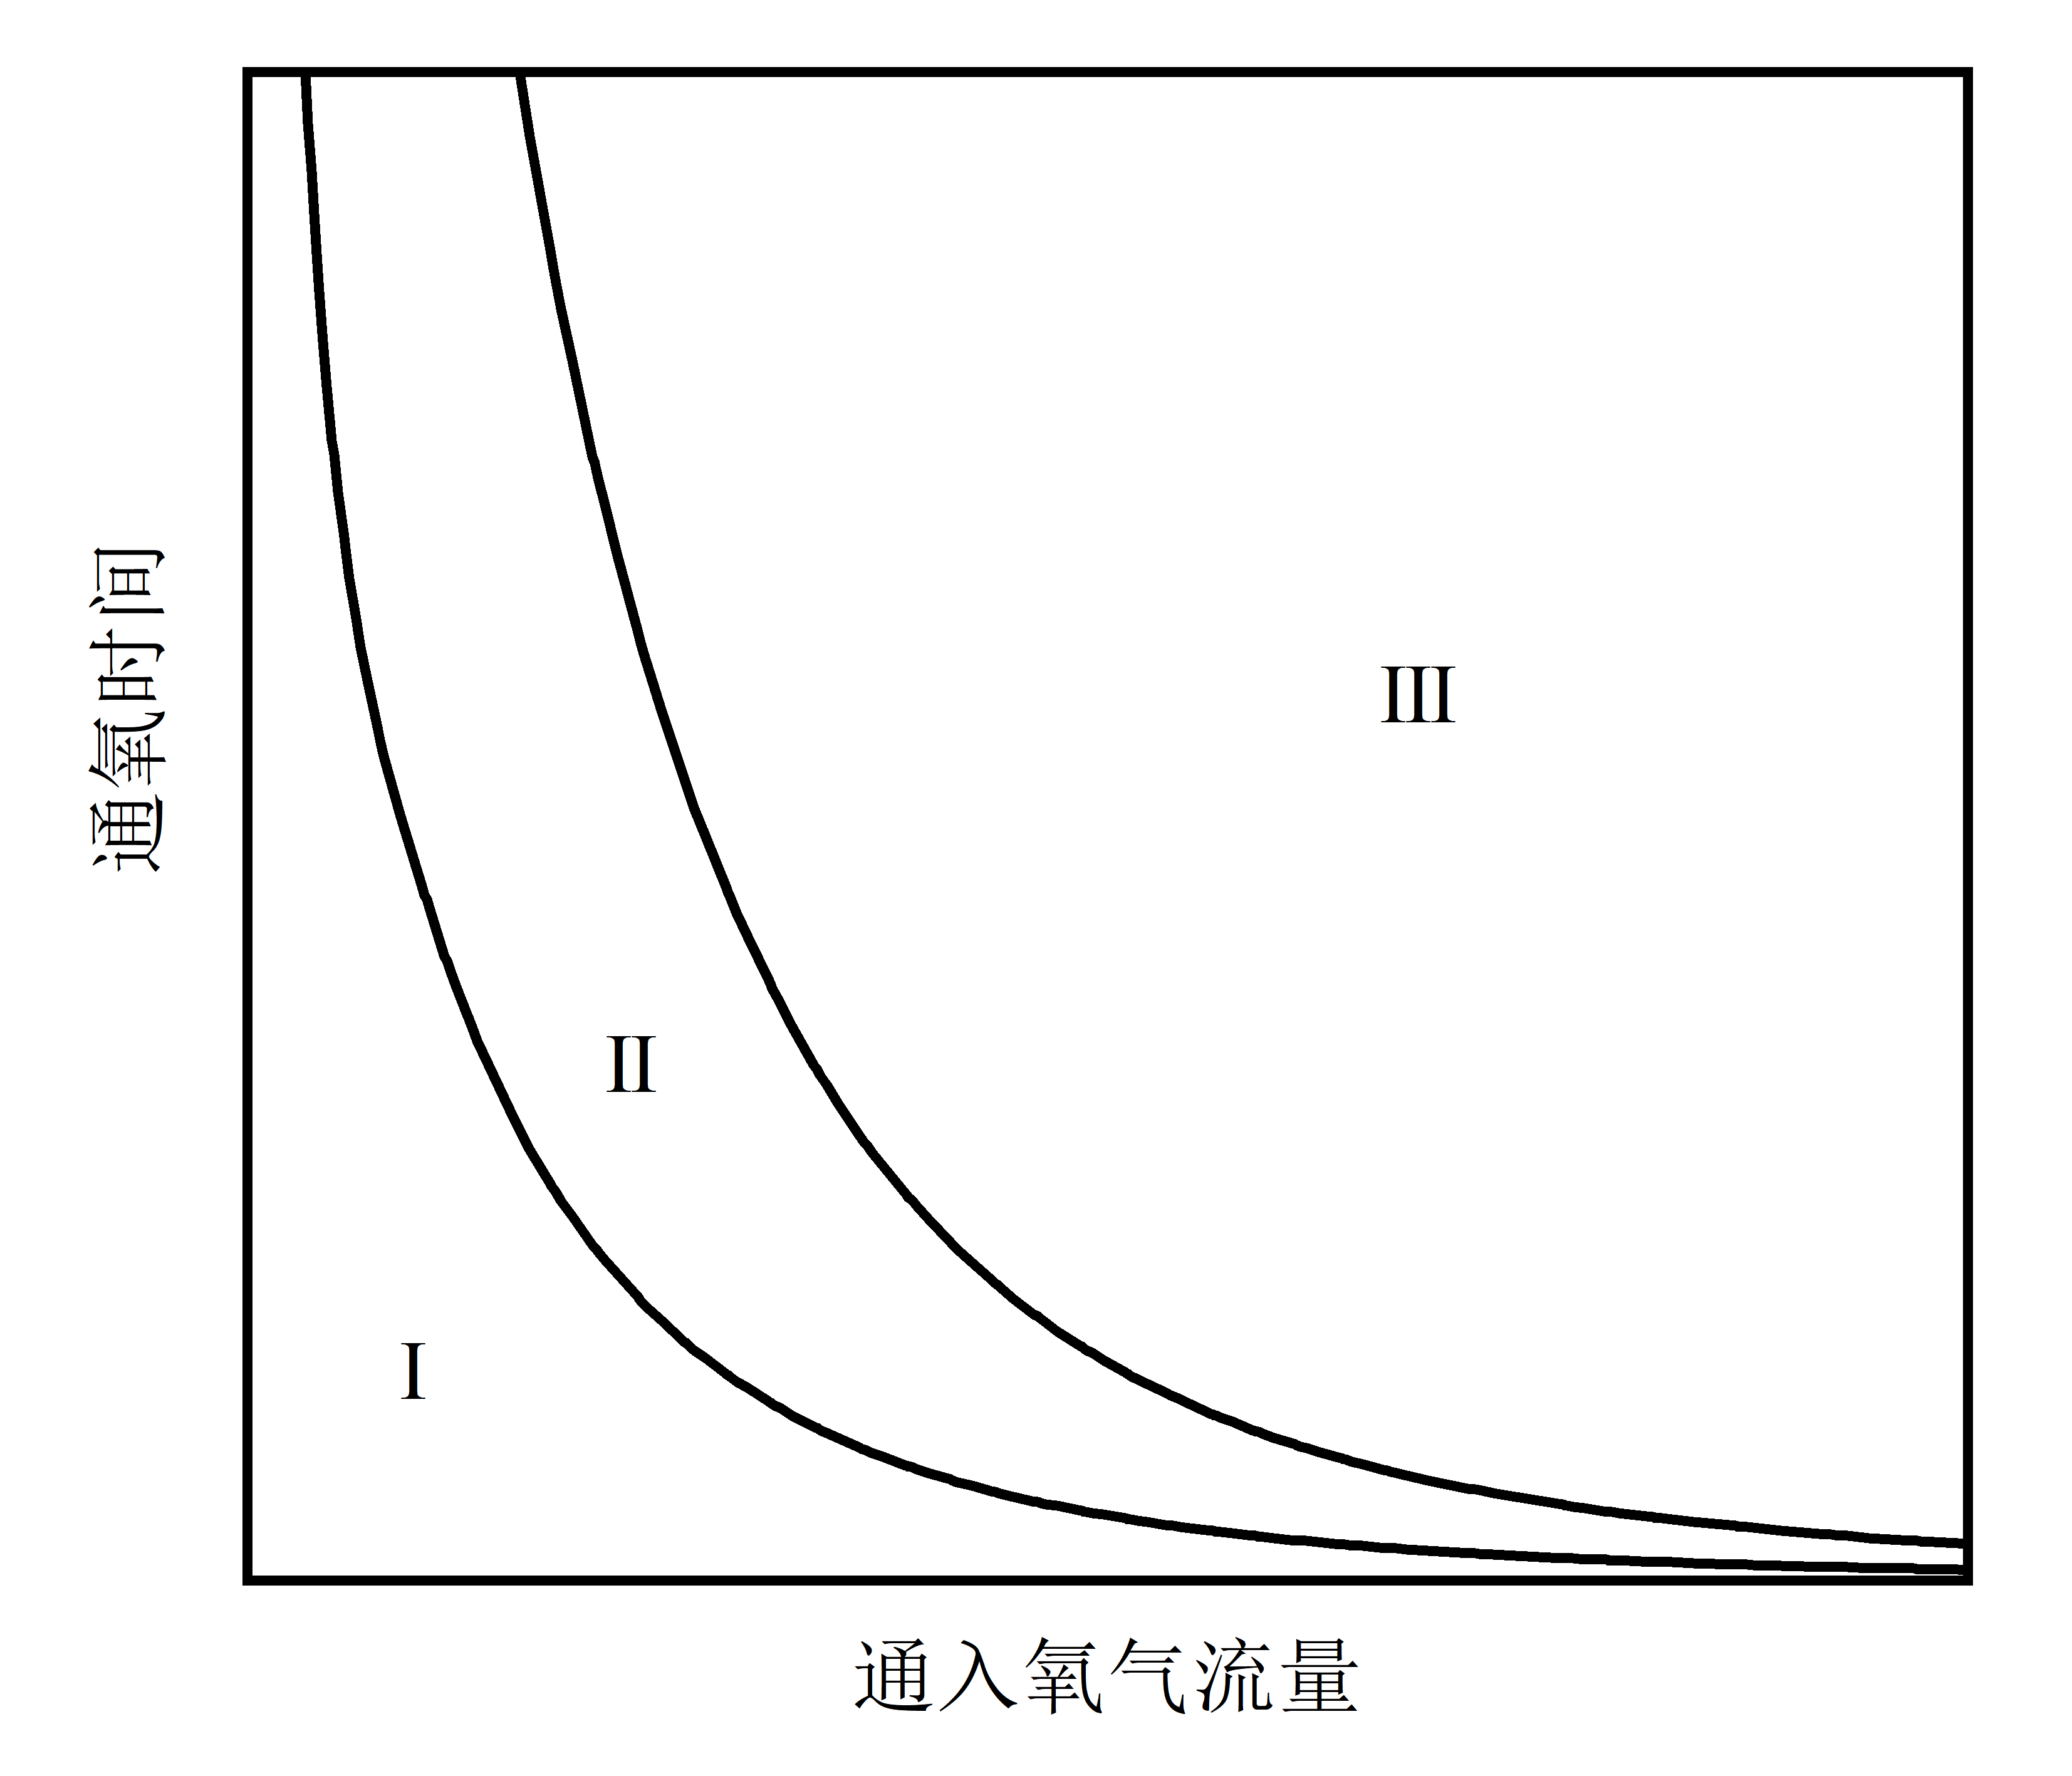
\includegraphics[]{pic/FLG_model_modePhase.png}
        \label{fig:FLG_model_modePhase}
    }
    \caption{氧辅助石墨烯蚀刻和生长作用及模式切换相图。(a)氧辅助石墨烯蚀刻和生长作用的平均反应速率;(b)氧调控的石墨烯蚀刻/生长的模式切换相图。其中,模式I为石墨烯多层蚀刻;模式II为石墨烯多层生长;模式III为石墨烯蚀刻(包括石墨烯多层以及石墨烯单层)}
    \label{fig:FLG_model}
\end{figure}

\section{本章小结}
本章结合多尺度理论计算和建模的方法,对化学气相沉积生长石墨烯过程中衬底形貌和生长气氛对于的石墨烯生长行为的影响进行了研究。研究表明衬底表面的台阶破坏了原衬底表面的对称性,为石墨烯的成核生长提供了优先生长位点和优先生长方向,使得石墨烯能够在多晶\cemb{Cu}的表面实现自发的多点定向成核生长。对于多晶\cemb{Cu}衬底表面石墨烯定向生长的研究有利于进一步消除石墨烯畴之间的晶界,实现大面积石墨烯单晶的低成本快速生长。而对于生长气氛的影响,研究显示氧的引入同时促进了石墨烯多层蚀刻和多层生长的反应。氧气对石墨烯多层的蚀刻和穿透作用的相互竞争突破了原有\cemb{Cu}衬底上石墨烯生长的自限制作用,导致了石墨烯多层交替出现蚀刻和生长的现象。结合气相动力学模拟和第一性原理计算,揭示了含氧气氛下氧气对于石墨烯多层生长和蚀刻速率的非均一促进作用和机理,建立了氧通量调控的石墨烯多层模式切换模型。石墨烯多层点生长模式的氧调控机制的发现有利于实现石墨烯的层数可控生长。本章对于化学气相沉积生长石墨烯的生长机理研究对于黑磷、六方氮化硼等二维材料的定向生长和层数调控生长机理具有一定的启发性。

    \chapter{极性锑化铟的生长机理研究}
\section{引言}
III-V族化合物半导体被认为是下一代电子器件和光电子器件有利的材料候选。以III-V族化合物半导体\cemb{InSb}为例,块体状态的\cemb{InSb}具有较小的带隙和极高的电子迁移能力\citing{RN919-2019, RN897-1984, RN898-2020}。当结构尺度减小至低维,\cemb{InSb}展现出了更多新颖的物理特性,如非常强的自旋-轨道作用\citing{RN887-2021, RN922-2010, RN924-2015},较大的朗德g(Landé g-factor)因子\citing{RN925-2008}以及二维电子气等\citing{RN899-2020, RN926-2021}。这些新颖的物理特性使得低维\cemb{InSb}纳米结构可以用于自旋电子\citing{RN927-2017, RN928-2020},拓扑量子计算等量子器件的构建\citing{RN946-2017, RN737-2015, RN921-2016, RN933-2015}。同时,III-V族化合物半导体的单层化也有研究者进行了稳定性以及电子特性研究\citing{RN918-2013}。

在\ref{cap:石墨烯的生长机理研究}中,我们计算了石墨烯在化学气相沉积环境下的生长机理。以石墨烯为代表的单元素平面二维材料,在理想的晶格状态下所有原子都处于同一平面,具有平面外方向的镜面对称性和反演对称性\citing{RN664-2017, RN903-2021}。而对于晶格结构以闪锌矿(zinc blende,ZB)和纤锌矿(wurtzite,WZ)为主的III-V族化合物半导体,其晶格对称性决定了在<111>晶向缺少反演对称。反演对称性的破缺使得III-V族化合物半导体的(111)晶面具有两个不同的端面,即以III族元素为端点的III极性和以V族元素为端点的V极性。不同极性表面原子的不同导致了III-V化合物半导体不同极性的(111)面表现出不同的物理化学特性\citing{RN910-2004}。III-V化合物半导体的表面极性同时也对生长过程中的III-V化合物的生长机理以及生长形貌产生影响\citing{RN929-2015, RN916-2018}。先前的研究表明,\cemb{InSb(111)}表面的许多新奇的物理现象与所处的极性息息相关。例如在特定极性的\cemb{InSb(111)}表面可以异质外延生长具有优异电子性质的新型材料 \citing{RN902-2016, RN852-2021, RN901-2019, RN900-2017, RN891-2019}。

分子束外延(molecular beam epitaxy,MBE)技术以及各种高级材料观测技术(如球差矫正透射电子显微镜)的发展使得研究者能够进一步研究III-V化合物半导体生长过程中极性的演化及调控手段。1994年,研究者发现在\cemb{InSb/Sn/InSb}异质结构中,底端\cemb{InSb}的极性可以透过5原子层的\cemb{Sn}薄膜,对上层的\cemb{InSb}的极性产生影响。随后的研究发现,大多数的III-V化合物半导体倾向于生长V极性的纳米结构\citing{RN864-2019, RN930-1998, RN931-2010},通过不同的生长手段,也有研究者生长出了III极性的表面\citing{RN930-1998, RN931-2010}。通过对实验参数和生长环境进行细致的控制,研究者能够利用分子束外延的方法对所合成的III-V化合物半导体纳米结构进行生长极性控制 \citing{RN913-2016, RN858-2019, RN889-2011, RN911-2019}。得益于合成技术的发展,研究者对于III-V半导体的生长机制进行了大量的实验观测和理论探究,力图对其中的极性演化规律产生更深的理解,从而能够更好的对III-V化合物半导体低维纳米结构进行定极性生长\citing{RN878-2020, RN940-1979, RN936-2002, RN886-2021, RN932-2018, RN894-2012, RN934-2018, RN941-2016}。

在本章中,以III-V族化合物半导体\cemb{InSb}为例,我们系统的探究了双层\cemb{InSb(111)}在\cemb{Bi(001)}衬底上的生长序列以及形貌演化规律。我们的研究表明在\cemb{Bi}衬底上,\cemb{InSb}的极化从第二层生长开始。单层的\cemb{InSb}在在\cemb{Bi}衬底上表现出非晶的形态。我们绘制了双层\cemb{InSb}在
\cemb{Bi}衬底上的极化相图,并且探究了从单层到双层\cemb{InSb}表面极性变化的物理成因。
\section{计算细节}
在本章中,密度泛函理论主要使用Vienna ab-initio Simulation Package (VASP) 软件包进行计算\citing{RN681-1996, RN682-1996}。在密度泛函理论计算中,我们使用广义梯度近似(GGA)下的Perdew-Burke-Ernzerhof (PBE)泛函描述电子之间的交换关联作用\citing{RN683-1996}。平面波的截断动能取为为$\SI{500}{\electronvolt}$。\cemb{InSb(111)}与衬底\cemb{Bi(001)}之间的范德瓦尔斯作用使用Grimme的DFT-D3方法进行描述,并带有Becke-Johnson阻尼作用 \citing{RN937-2010, RN938-2011}。对于$1 \times 1$和$2 \times 2$大小的切片模型,我们使用以$\Gamma$ 点为中心的$11 \times 11 \times 1$和$7 \times 7 \times 1$的K空间采样网络进行布里渊区积分。而对于实空间体积更大的切片模型以及团簇模型,我们仅对$\Gamma$ 点进行采样。在原子结构优化的计算中,力收敛条件设为$\SI{1e-2}{\electronvolt \per \angstrom}$,电子结构自洽场计算的收敛条件设为$\SI{1e-6}{\electronvolt}$。对于过渡态的计算,我们采用CI-NEB(Climbing Image Nudged Elastic Band)方法对始末反应状态之间的能量鞍点进行搜寻,以确定反应势垒的大小\citing{RN790-2000}。对于过渡态计算,力收敛条件设为$\SI{3e-2}{\electronvolt \per \angstrom}$。

对于极性面的表面能,我们使用赝氢饱和法及四面体法进行计算\citing{RN300-2016}。用于表面能计算的\cemb{InSb}切片模型以及四面体模型均基于优化过的块体\cemb{InSb},并进行了进一步的结构优化。计算表面能的切片模型的大小为$2 \times 2$,包含至少9层\cemb{InSb(111)}双原子层。对于\cemb{InSb(111)/Bi(001)}体系,我们是由六层\cemb{Bi(001)}双原子层作为衬底。衬底底面原子在优化过程中固定在块体构型,用以模拟半无限衬底。在\cemb{Bi(001)}表面,\cemb{InSb(111)}覆盖层的晶格由于约$\SI{1.9}{\percent}$等晶格失配而有微小的形变。切片模型的垂直表面方向放置至少$\SI{20}{\angstrom}$的真空层以防止周期性条件相邻切片的影响。在我们的计算中,块体\cemb{InSb}和块体\cemb{Bi}的晶格常数分别为\SI{6.62}{\angstrom}和\SI{4.79}{\angstrom},与先前文献报道一致\citing{RN939-2013,RN1266-1965}。

为了估计原子之间的作用强弱,我们使用LOBSTER软件包对晶体轨道哈密顿量布居(Crystal Orbital Hamilton Population, COHP)进行了计算和分析\citing{RN951-2011, RN950-1993, RN949-2016}。在本章中,\cemb{InSb(111)/Bi(001)}体系中的成键强弱由-COHP谱和-COHP积分(-ICOHP)进行量化。-ICOHP由-COHP谱中的电子占据态积分而来。在-COHP和-ICOHP中,成键态以正值表示,反键态以负值表示。
\section{单层锑化铟的生长机理}

\subsection{\cemb{Bi(001)}衬底表面锑、铟原子的吸附机理}
\def\TfourSite{\rm T_{4} \it}
\def\HthreeSite{\rm H_{3} \it}
\def\mievpas{\milli\electronvolt\per\angstrom\squared}
\def\InSbMLpolar#1#2{\rm #1-In/#2-Sb}
\def\NumOfAdatom{\it N_{\rm adatoms} \it}
\def\CNinNsb#1#2#3#4{\rm #1/#2{}^{#3InV}_{#4SbT} \it}

对于\cemb{InSb(111)}极性面在\cemb{Bi(001)}衬底表面的生长机理,我们首先对衬底表面锑、铟原子的吸附进行研究。在衬底表面,吸附原子的结合能$\energyVar{b}{}$为\chinesecolon
\[
    \energyVar{b}{}=\left(\energyVar{sub+adatom}{}-\energyVar{sub}{}-N\muVar{adatom}{}\right)/ N
\]

其中,$\energyVar{sub+adatom}{}$和$\energyVar{sub}{}$为吸附有原子的衬底和未吸附原子的衬底的能量。$\muVar{adatom}{}$为吸附原子的化学势。$N$为吸附原子的总数。

我们考虑\cemb{In}和\cemb{Sb}吸附原子在\cemb{Bi(001)}表面吸附覆盖率为$1/ 4$的结合能,计算结果如\ref{fig:IS_Bi_adatoms}所示。根据我们的计算,\cemb{In}原子和\cemb{Sb}原子都更倾向于吸附在\cemb{Bi(001)}衬底表面的$\TfourSite$位和$\HthreeSite$位。如图\ref{fig:IS_structure_T4onBi}和\ref{fig:IS_structure_H3onBi}所示,$\TfourSite$为\cemb{Bi(001)}衬底表面的四重配位顶位,正对于第一层\cemb{Bi}双原子层的下层原子。$HthreeSite$为\cemb{Bi(001)}衬底表面的三种配位空心位,正对于第一层\cemb{Bi}双原子层的空心以及第二层\cemb{Bi}双原子层的上层原子。\cemb{In}原子和\cemb{Sb}原子在\cemb{Bi(001)}衬底表面的吸附能如图\ref{fig:IS_DFT_adatomBind}所示,计算表明\cemb{Bi(001)}衬底表面的$\TfourSite$为\cemb{In}原子和\cemb{Sb}原子的最佳吸附位点。而$\HthreeSite$为二者的次优吸附位点。在吸附能以及后续的能量计算中,我们使用\cemb{In}的化学势$\muVar{In}{}$来表示\cemb{In}元素在生长气氛中的活性水平,体现在\cemb{InSb}化学平衡下\cemb{In}元素和\cemb{Sb}元素的浓度差距。

\begin{figure}[htb]
    \subfloat[]{
        \label{fig:IS_DFT_adatomBind}
        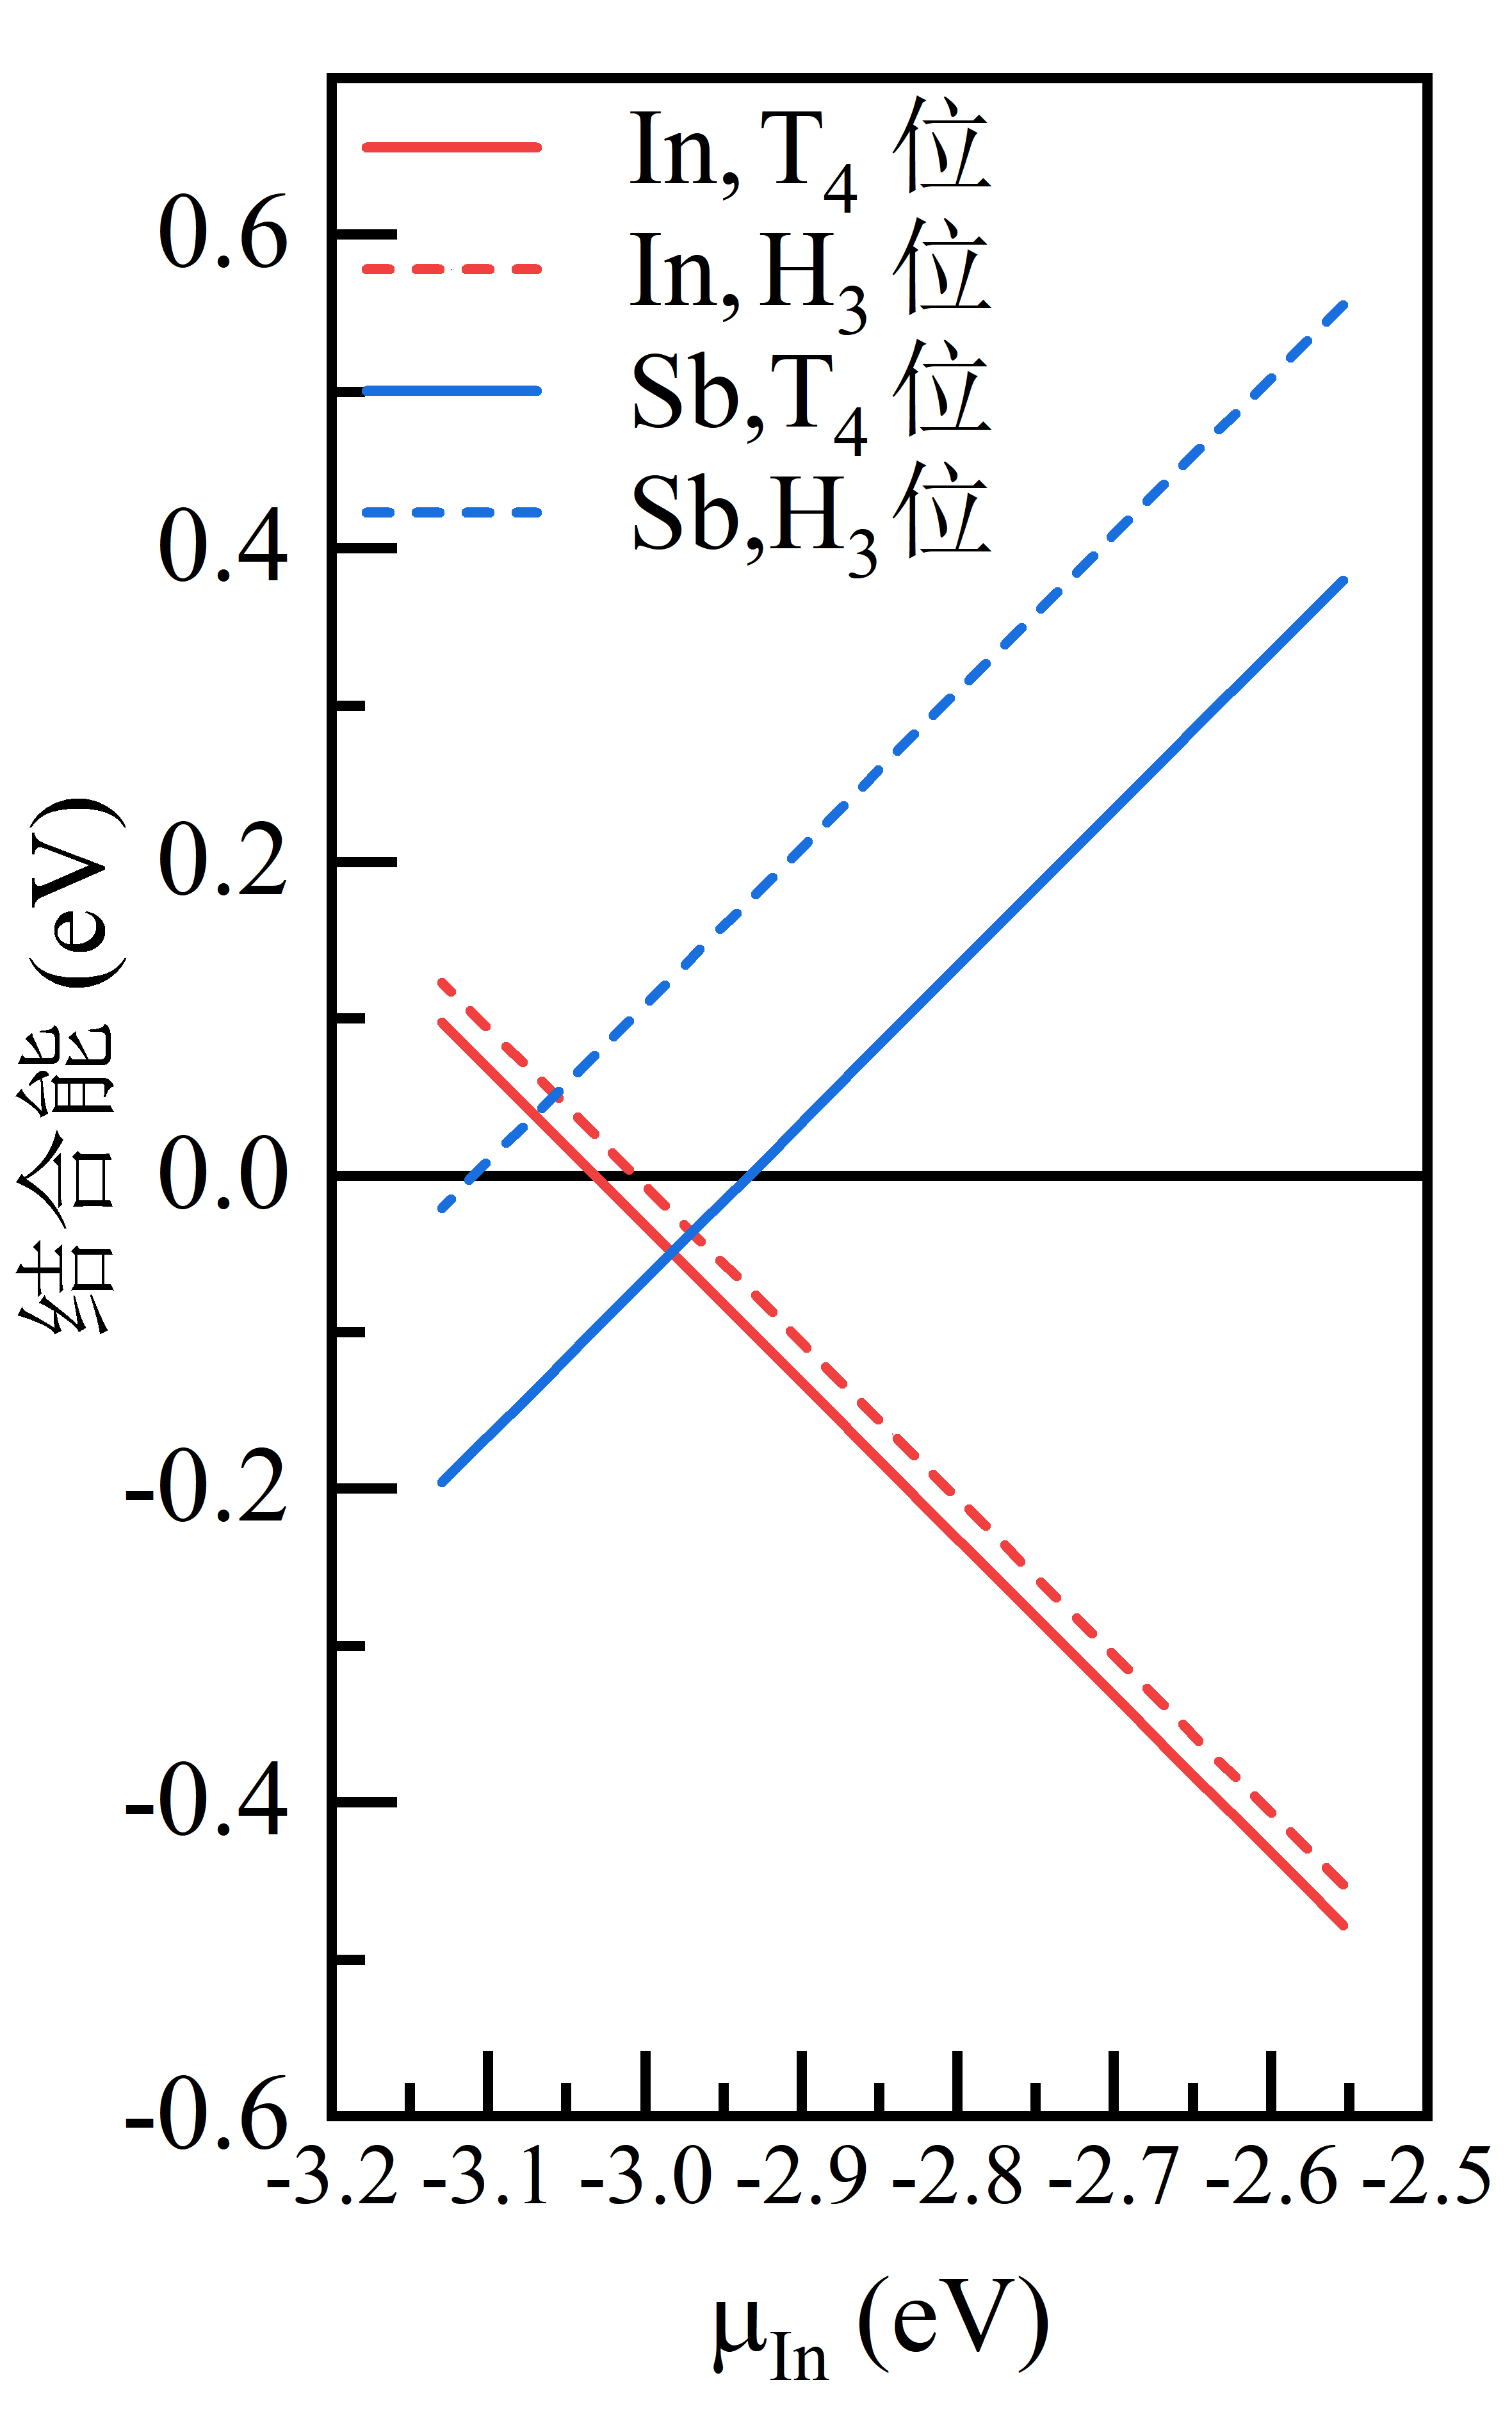
\includegraphics[]{pic/IS_DFT_adatomBind.png}
    }
    \subfloat[]{
        \label{fig:IS_structure_T4onBi}
        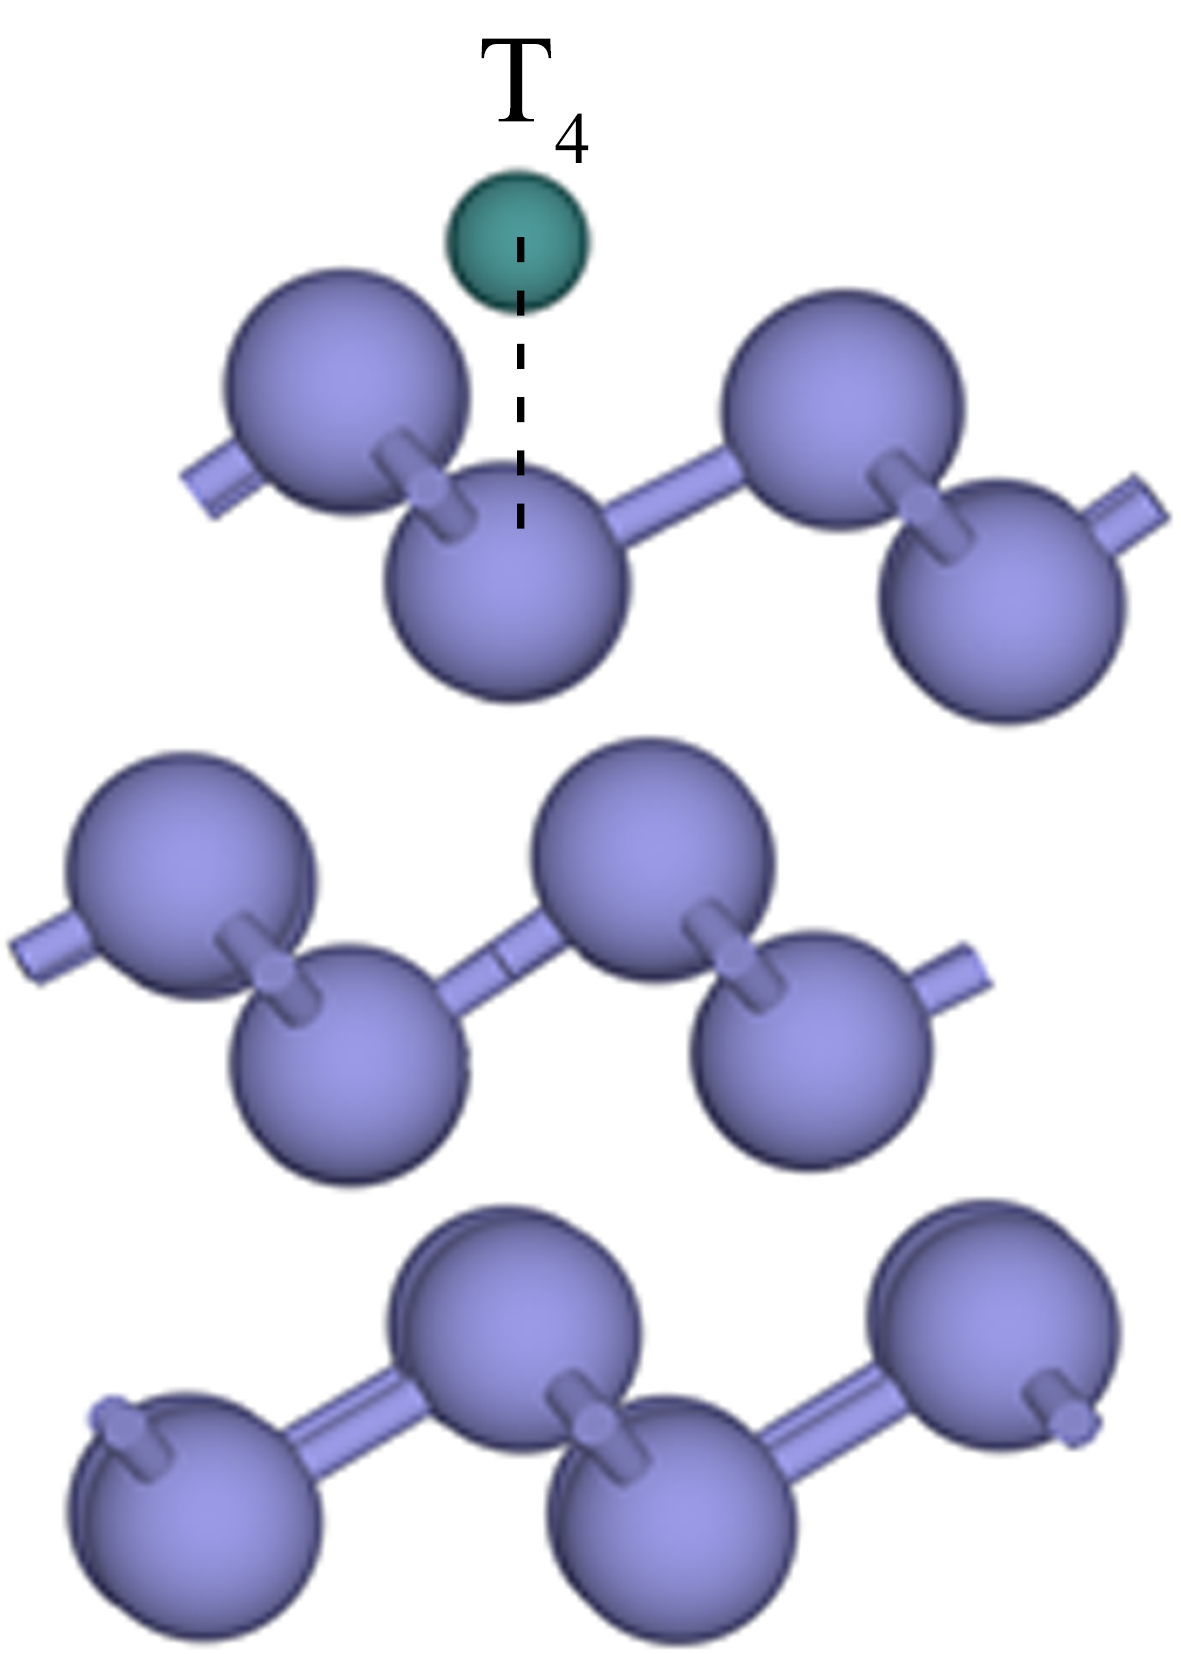
\includegraphics[width=0.3\textwidth,trim={0, -20, 0 0},clip]{pic/IS_structure_T4onBi.png}
    }
    \subfloat[]{
        \label{fig:IS_structure_H3onBi}
        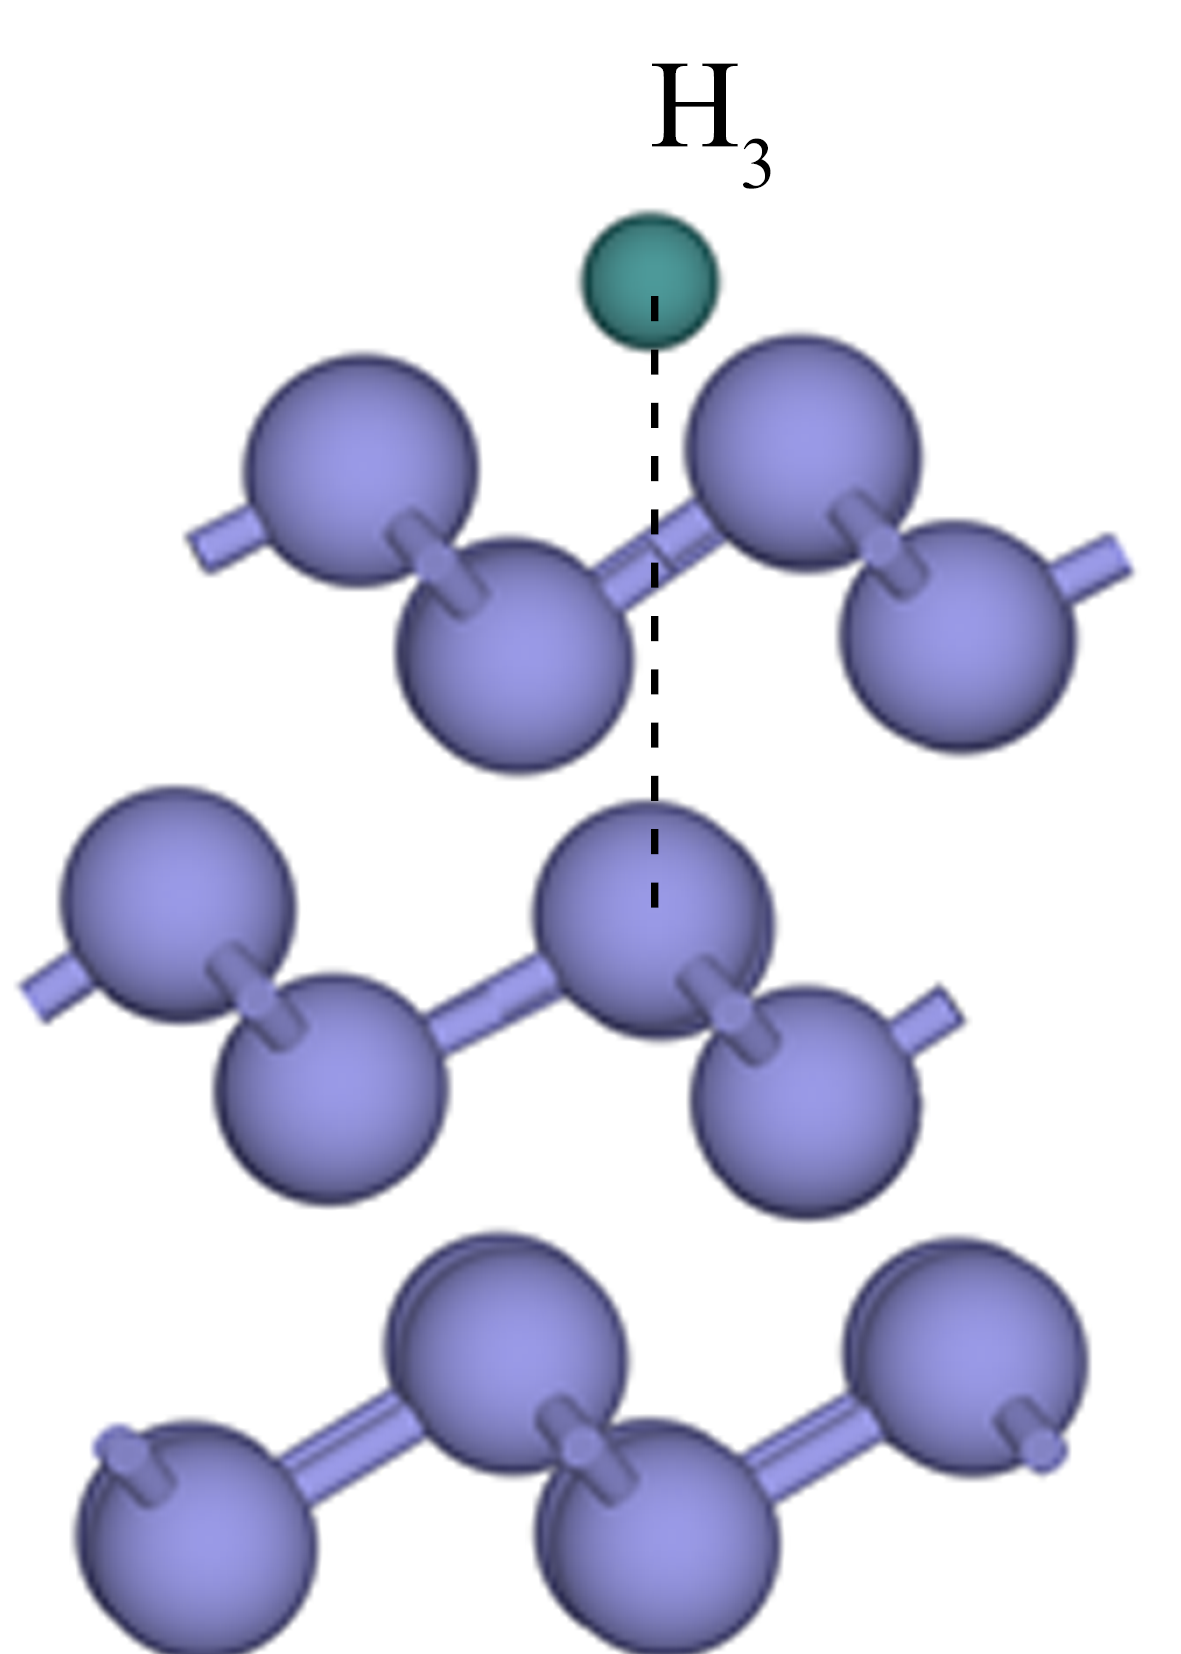
\includegraphics[width=0.3\textwidth,trim={0, -20, 0 0},clip]{pic/IS_structure_H3onBi.png}
    }
    \caption{\cemb{Bi(001)}衬底表面\cemb{In}和\cemb{Sb}吸附原子的结合能和吸附位点。(a)吸附原子结合能;(b)吸附位点T4;(c)吸附位点H3。 原子结构图中,\cemb{Bi}原子使用蓝色表示,吸附原子(\cemb{In}、\cemb{Sb})用绿色表示。}
    \label{fig:IS_Bi_adatoms}
\end{figure}

对于$\muVar{adatom}{}$为吸附原子的化学势,由于生长环境下\cemb{InSb}块体的化学平衡,我们有\chinesecolon
\begin{equation}
    \label{eq:IS_bulkEqmb}
    \muVar{In}{}+\muVar{Sb}{}=\energyVar{InSb}{tot}=\energyVar{In\left(Bulk\right)}{}+\energyVar{Sb\left(Bulk\right)}{}+\Delta H_{f}\left(\cemb{InSb}\right)
\end{equation}

其中$\energyVar{InSb}{tot}$、$\energyVar{In\left(Bulk\right)}{}$和$\energyVar{Sb\left(Bulk\right)}{}$为\cemb{InSb}块体,\cemb{In}块体和\cemb{Sb}块体的能量。因此,在生长气氛中\cemb{InSb}的化学平衡下,$\muVar{In}{}$的变化范围为$\muVar{In}{}\leqslant \energyVar{Sb\left(Bulk\right)}{}+\Delta H_{\rm f}\left(\cemb{InSb}\right) \leqslant \energyVar{In\left(Bulk\right)}{}$,代表\cemb{In}的化学势$\muVar{In}{}$由纯\cemb{Sb}的生长环境变化到纯\cemb{In}的生长环境。

对于吸附在$\TfourSite$位点的\cemb{In}原子,计算所得的在纯\cemb{In}环境下的结合能为\SI{-0.48}{\electronvolt},低于在纯\cemb{Sb}环境下同样吸附在$\TfourSite$位点的\cemb{Sb}原子的结合能(\SI{-0.19}{\electronvolt})。更抵的结合能意味着相比于\cemb{Sb}原子,在能量最低的驱动下有更多的\cemb{In}原子从块体的状态分离并以吸附原子的状态沉积到\cemb{Bi(001)}的表面。对于\cemb{In}原子来说,其在最优吸附位点$\TfourSite$的结合能只比吸附次优吸附位点$\HthreeSite$的结合能低\SI{0.026}{\electronvolt}。而对于\cemb{Sb}原子,其在次优吸附点$\HthreeSite$和最优吸附点$\TfourSite$之间的结合能之差为\SI{0.17}{\electronvolt}。由于\cemb{Sb}原子在次优吸附位点$\HthreeSite$较差的吸附能力,\cemb{Sb}原子只能在接近纯\cemb{Sb}的生长环境中在\cemb{Bi(001)}表面的$\HthreeSite$位点吸附。

进一步考虑生长环境中的化学计量比的变化对于原子吸附的影响。在图\ref{fig:IS_DFT_adatomBind}中可以看到,只有很小的$\muVar{In}{}$区间允许\cemb{In}和\cemb{Sb}同时在\cemb{Bi(001)}衬底表面吸附($\energyVar{f}{} \leqslant 0$)。在这个区间内\cemb{In}原子可以在$\TfourSite$和$\HthreeSite$位点吸附,而\cemb{Sb}原子只能在$\HthreeSite$位点吸附。对于\cemb{In}原子,由于较低的吸附能,相比于\cemb{Sb}原子其能够在较宽的$\muVar{In}{}$区间内在\cemb{Sb}衬底表面吸附。当环境中的\cemb{In}原子化学势稍微向纯\cemb{In}环境倾斜时($\muVar{In}{}\geqslant \SI{-2.9}{\electronvolt}$),仅有\cemb{In}能够在\cemb{Bi}的表面吸附,而\cemb{Sb}原子则由于大于零的结合能倾向于从\cemb{Bi}的表面脱附。

由于\cemb{In}原子和\cemb{Sb}原子在\cemb{Bi(001)}表面不同的吸附行为,在相同的化学气氛下,\cemb{In}和\cemb{Sb}很难同时在\cemb{Bi}衬底的表面独立吸附。出于更高的吸附能力,\cemb{In}在\cemb{InSb}的初期成核生长过程中处于更加主导的地位。在\cemb{In}原子能够沉积的区域,气氛中的\cemb{Sb}原子需要与已吸附的\cemb{In}原子成键、成核,才能够在\cemb{Bi}衬底的表面形成\cemb{InSb}。

我们进一步计算了\cemb{In}和\cemb{Sb}原子吸附在\cemb{Bi(001)}表面后的迁移势垒。如图\ref{fig:IS_DFT_adatomDiff}所示,对于吸附在\cemb{Bi}衬底表面的\cemb{In},其在两个等效的最优吸附$\TfourSite$位点之间迁移的势垒为\SI{0.20}{\electronvolt}。对于\cemb{Sb}原子,其在同样的最优位点$\TfourSite$之间的迁移势垒略低,为$\SI{0.19}{\electronvolt}$。而对于吸附在次优吸附位点$\HthreeSite$的\cemb{Sb}原子,只需要跨越\SI{0.018}{\electronvolt}的势垒就可迁移至最优的$\TfourSite$位点。吸附在$\HthreeSite$位点的\cemb{In}原子需要跨越约\SI{0.17}{\electronvolt}的势垒即可可迁移至能量更有优势的$\HthreeSite$位点。考虑到\cemb{In}原子在最优吸附位点$\TfourSite$和次优吸附位点$\HthreeSite$之间的能量差只有\SI{0.026}{\electronvolt},并且\cemb{In}原子和\cemb{Sb}原子在\cemb{Bi(001)}表面较低的迁移势垒,吸附的\cemb{In}原子在$\TfourSite$和$\HthreeSite$近似于均匀分布。而\cemb{Sb}原子由于在$\TfourSite$位点具有约\SI{0.17}{\electronvolt}的能量优势,因此\cemb{Sb}原子在$\TfourSite$位点吸附的比例较高。

\begin{figure}[htb]
    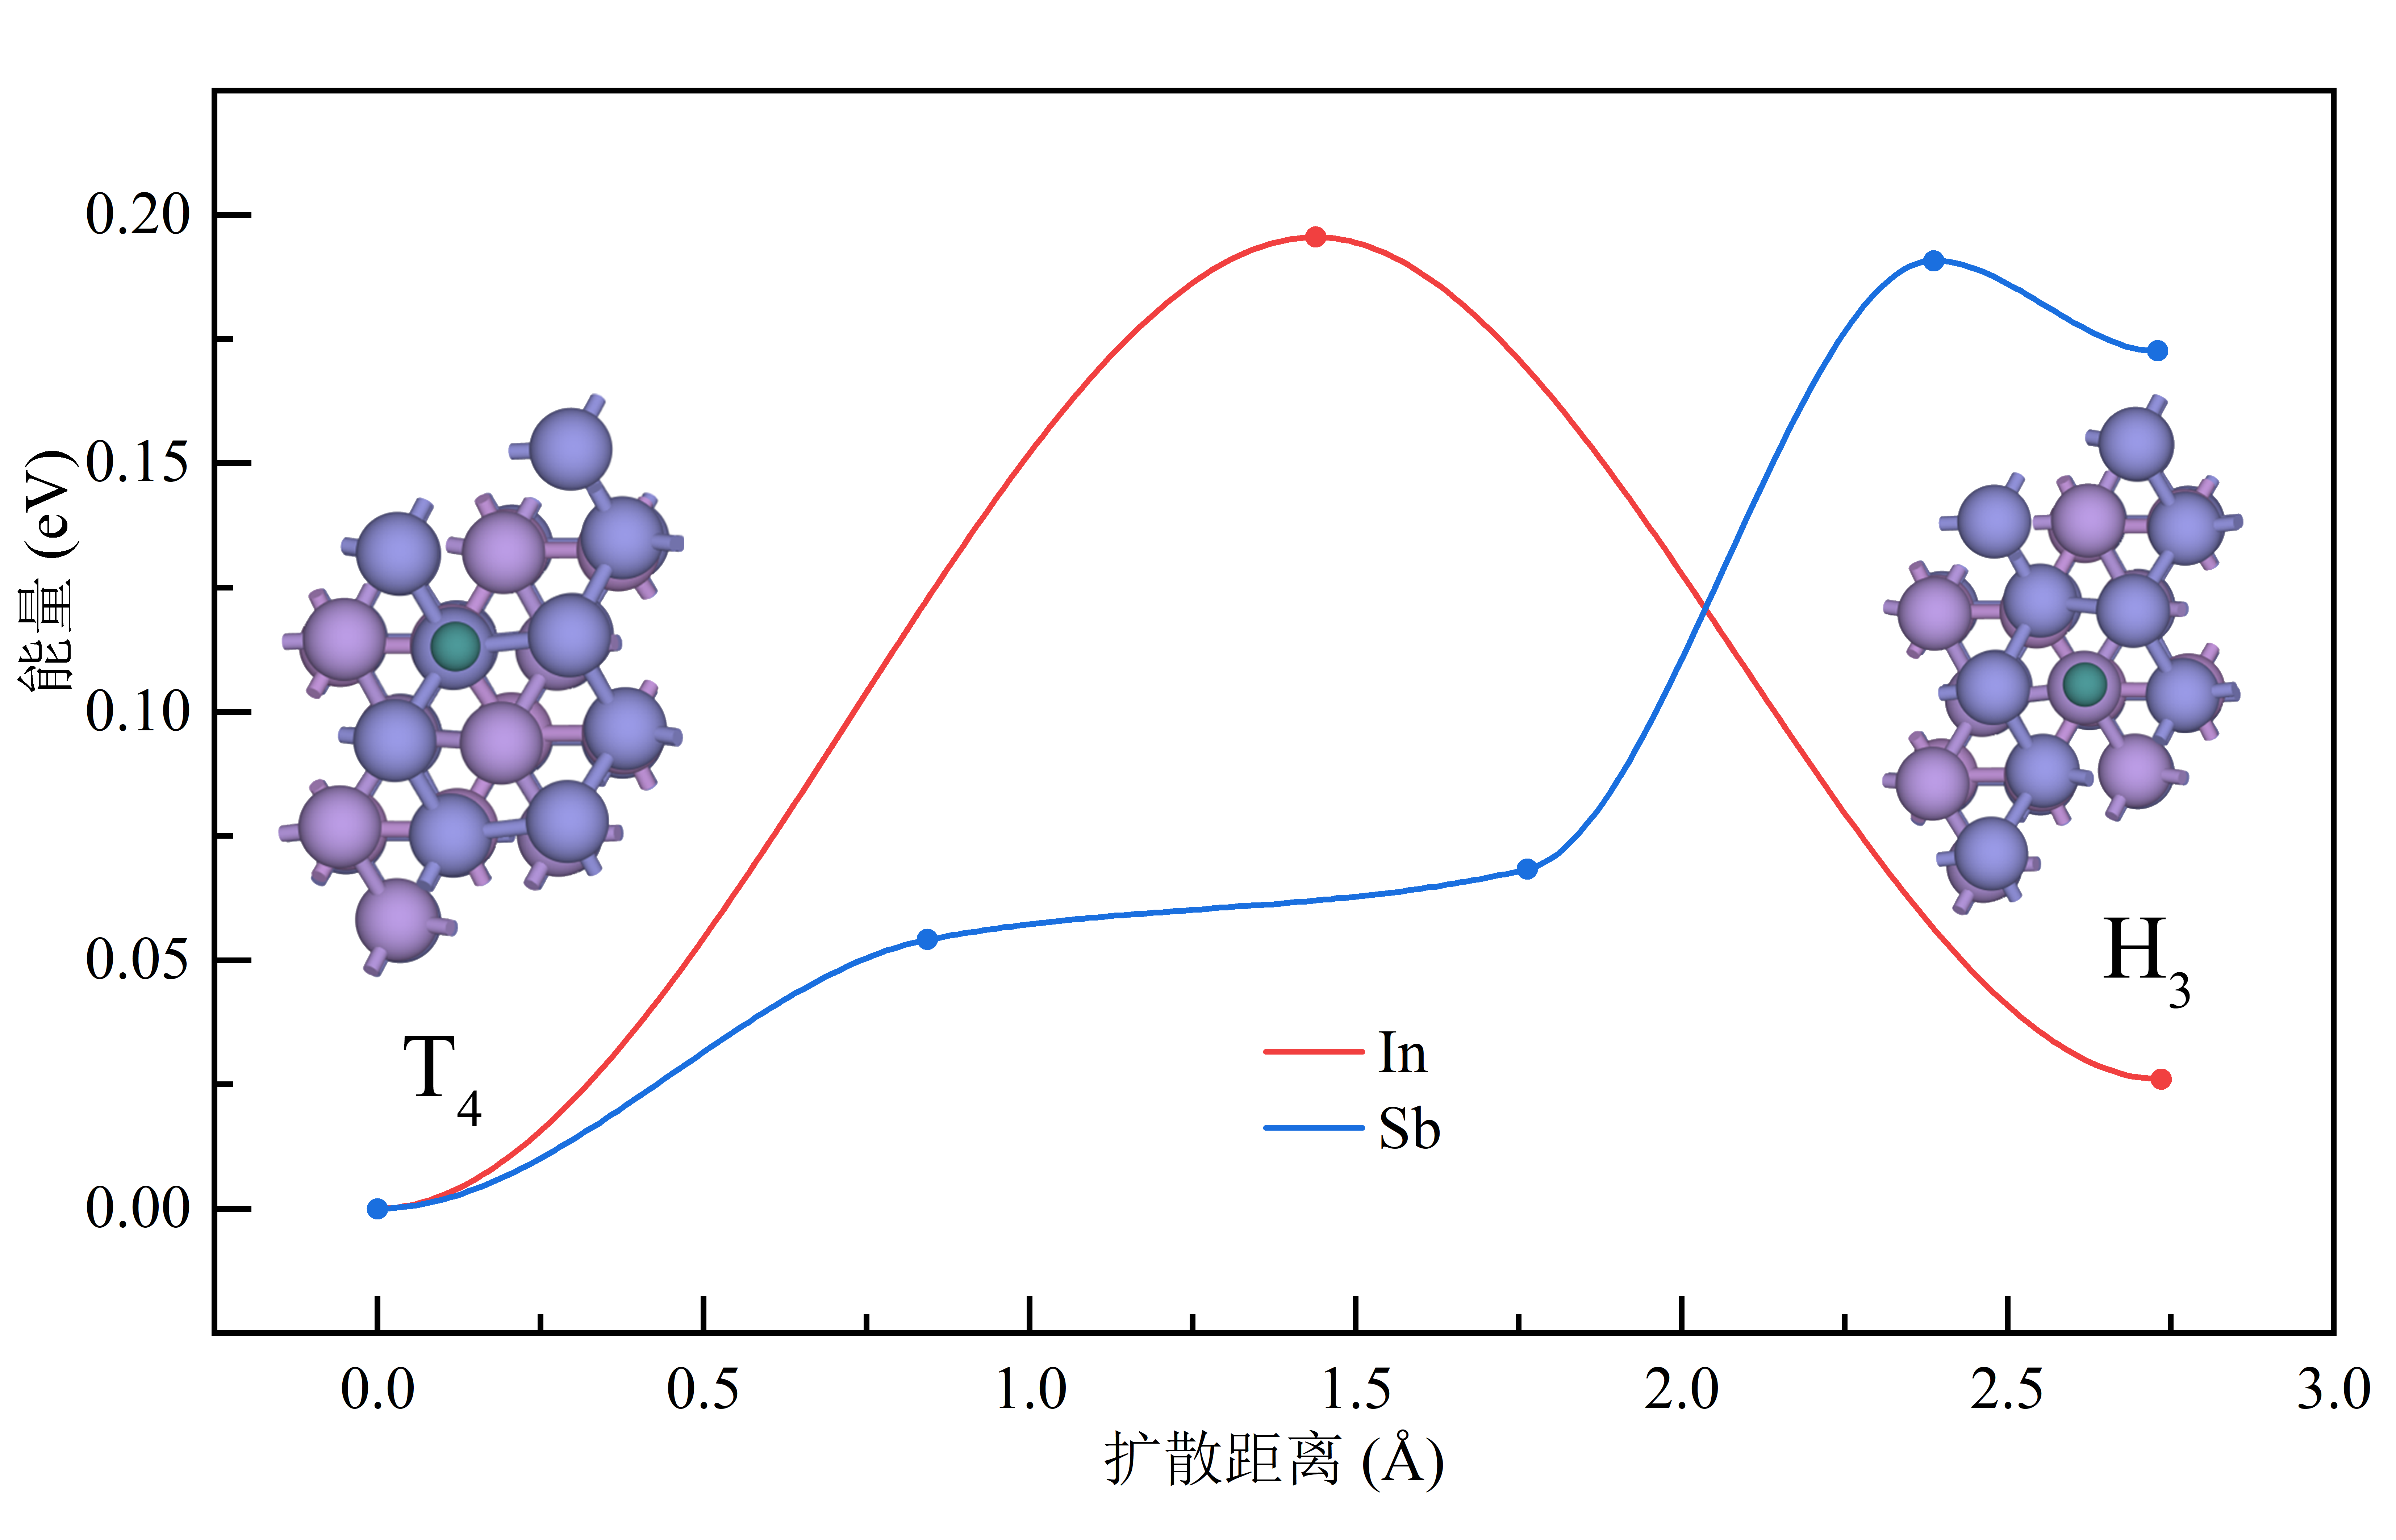
\includegraphics{pic/IS_DFT_adatomDiff.png}
    \caption{\cemb{Bi(001)}衬底表面\cemb{In}和\cemb{Sb}吸附原子的迁移势垒。原子结构图中,\cemb{Bi}原子使用蓝色表示,吸附原子(\cemb{In}、\cemb{Sb})用绿色表示。}
    \label{fig:IS_DFT_adatomDiff}
\end{figure}

为了能进一步探究\cemb{InSb(111)}在\cemb{Bi(001)}衬底上的层状生长机理以及极性的演化过程,我们计算了单层\cemb{InSb}在\cemb{Bi(001)}衬底上的形成能$\energyVar{f}{}$\chinesecolon
\begin{equation}
    \label{eq:IS_formationEnenrgy}
    \energyVar{f}{}=\frac{1}{\alpha}\left(\energyVar{\cemb{InSb}+sub}{}-\energyVar{sub}{}-N_{\rm In}\muVar{In}{}-N_{\rm Sb}\muVar{Sb}{}\right)
\end{equation}

其中,$\alpha$为模拟体系的表面积;$\energyVar{\cemb{InSb}+sub}{}$和$\energyVar{sub}{}$分别为在衬底表面生长了一层\cemb{InSb}的能量以及单独衬底的能量;$N_{\rm In}$和$N_{\rm Sb}$分别为\cemb{InSb}单层中\cemb{In}和\cemb{Sb}原子的数量。

我们首先考虑理想的\cemb{InSb}单层在\cemb{Bi(001)}衬底上的生长情况。在我们的计算中,无论是\cemb{In}极性的\cemb{InSb(111)}单层还是\cemb{Sb}极性,他们都倾向于在\cemb{Bi(001)}衬底表面形成面心立方的堆叠形式(fcc, ABC堆叠)。同时,这也与我们在单\cemb{In/Sb}原子的吸附计算结果一致,即\cemb{In}和\cemb{Sb}作为吸附原子更倾向于吸附在\cemb{Bi(001)}表面的$\TfourSite$位和$\HthreeSite$位。具体而言,\cemb{In}极性的\cemb{InSb(111)}单层在\cemb{Bi(001)}衬底的表面形成能为\SI{-13.74}{\mievpas},高于\cemb{Sb}极性\cemb{InSb(111)}单层的\SI{-9.40}{\mievpas}。因此,对于理想的\cemb{InSb}单层,在\cemb{Bi(001)}衬底上应生长为\cemb{In}极性。在表格\ref{tab:IS_idealInSb_formationEnergy}中,我们总结了不同极性的\cemb{InSb}单层在\cemb{Bi(001)}衬底上的形成能及原子分布。

\begin{table}[h]
    \centering
    \caption{不同极性的\cemb{InSb}单层在\cemb{Bi(001)}衬底上的形成能及原子分布}
    \begin{tabular}{cccc}
        \toprule
        极性          & 形成能(\si{\mievpas}) & \cemb{In}原子位置 & \cemb{Sb}原子位置 \\
        \midrule
        \cemb{In}极性 & -13.74                & $\TfourSite$      & $\HthreeSite$     \\
        \cemb{Sb}极性 & -9.40                 & $\HthreeSite$     & $\TfourSite$      \\
        \bottomrule
    \end{tabular}
    \label{tab:IS_idealInSb_formationEnergy}
\end{table}

\subsection{单层锑化铟的极性演化}

\begin{figure}[htb]
    \subfloat[]{
        \label{fig:IS_structure_1Linsb_04}
        \begin{tabular}{c}
            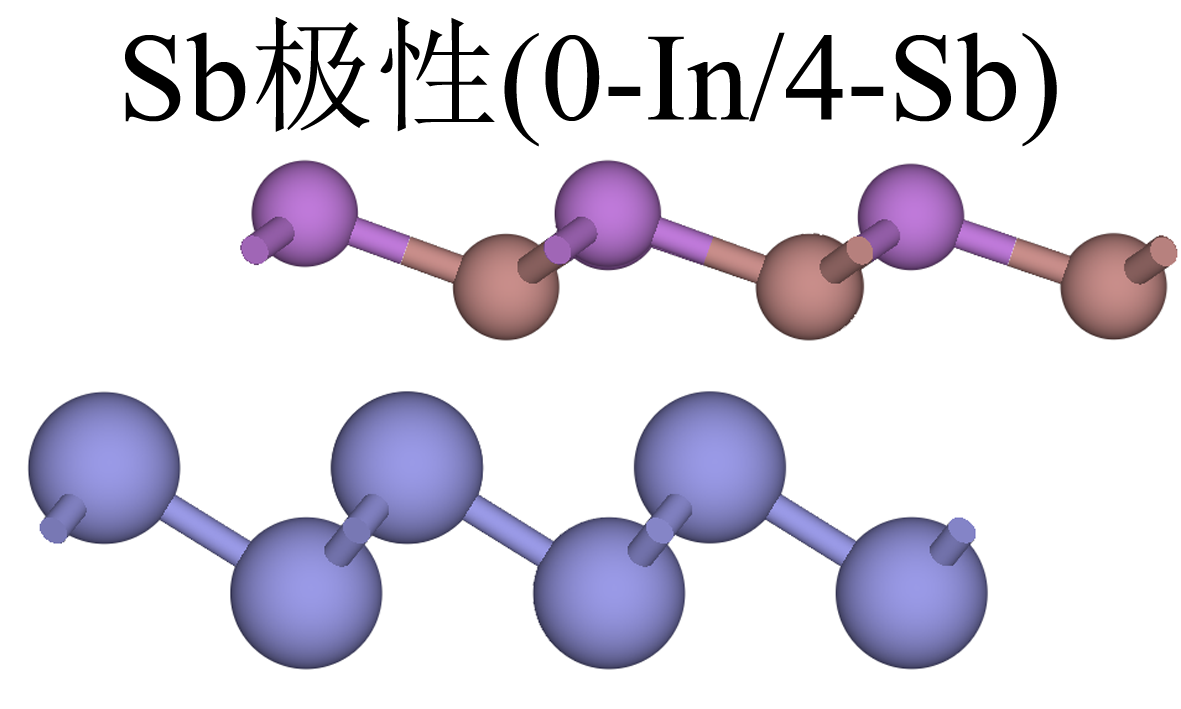
\includegraphics[width=0.28\textwidth]{pic/IS_structure_1Linsb_04side.png} \\
            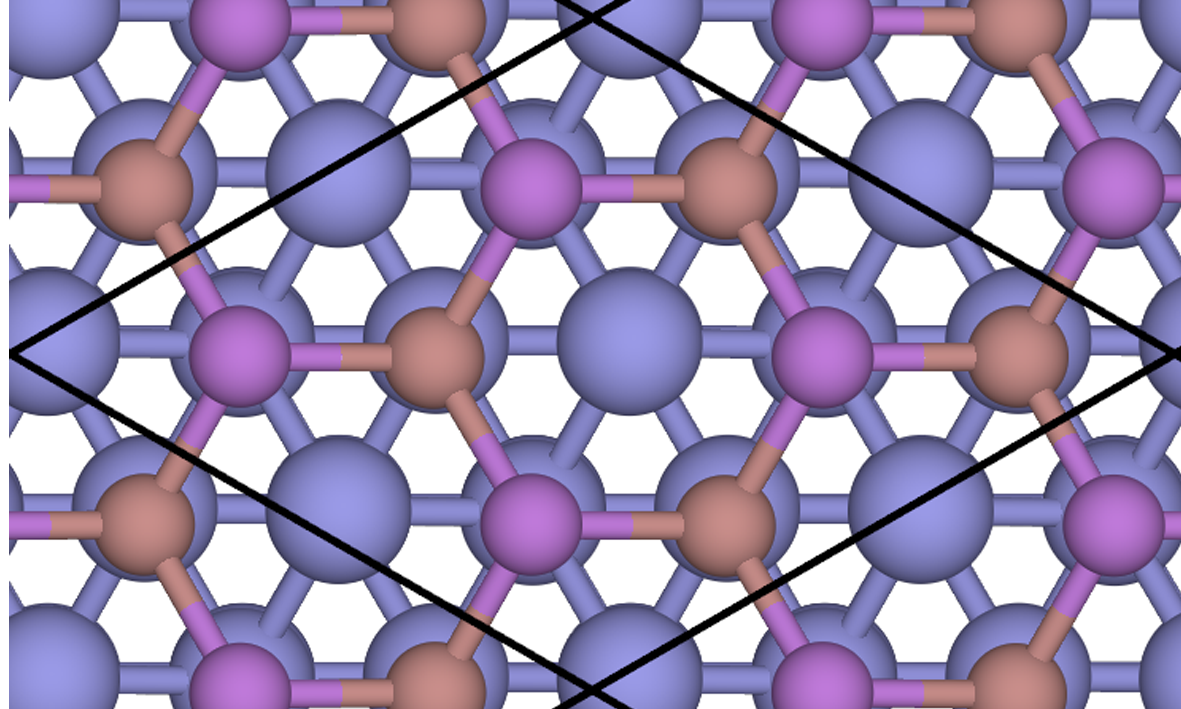
\includegraphics[width=0.28\textwidth]{pic/IS_structure_1Linsb_04top.png}
        \end{tabular}
    }
    \subfloat[]{
        \label{fig:IS_structure_1Linsb_13}
        \begin{tabular}{c}
            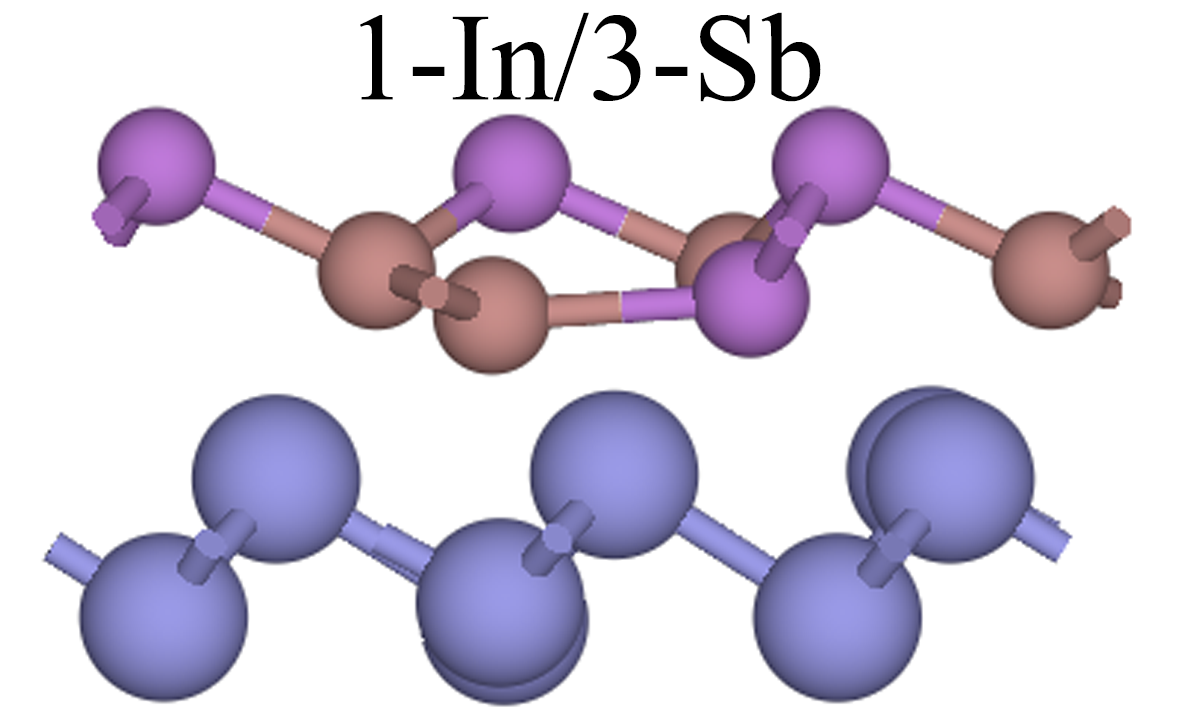
\includegraphics[width=0.28\textwidth]{pic/IS_structure_1Linsb_13side.png} \\
            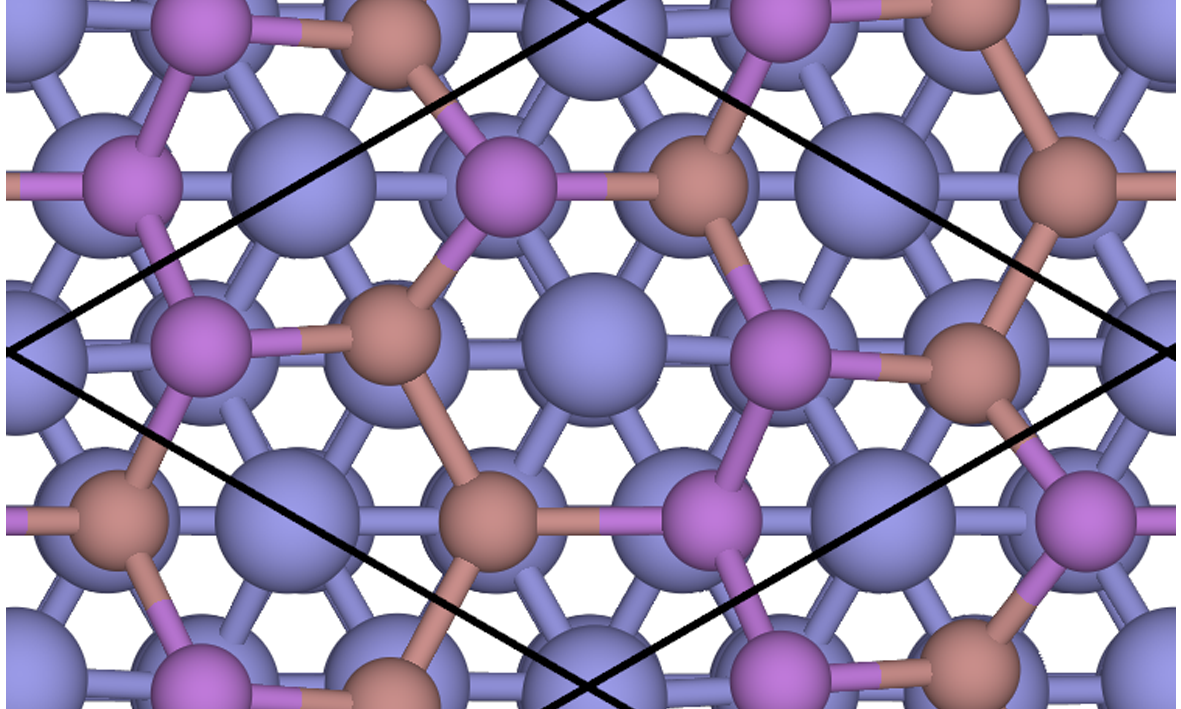
\includegraphics[width=0.28\textwidth]{pic/IS_structure_1Linsb_13top.png}
        \end{tabular}
    }
    \subfloat[]{
        \label{fig:IS_structure_1Linsb_22rec}
        \begin{tabular}{c}
            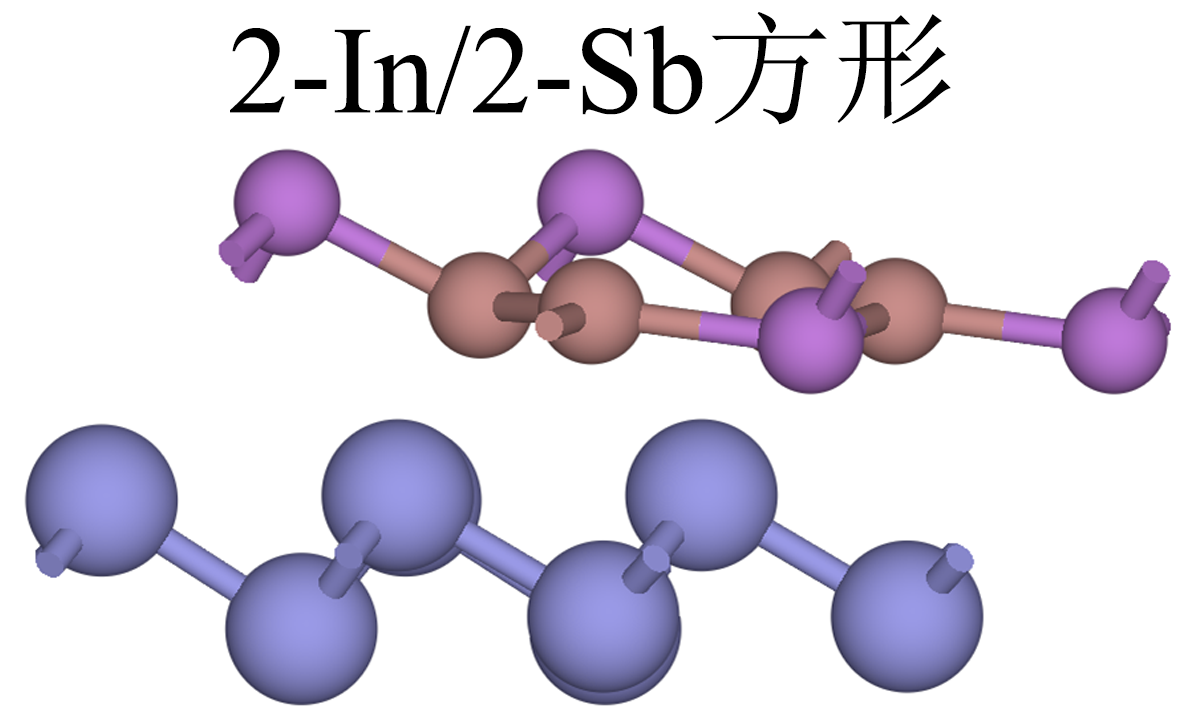
\includegraphics[width=0.28\textwidth]{pic/IS_structure_1Linsb_22recside.png} \\
            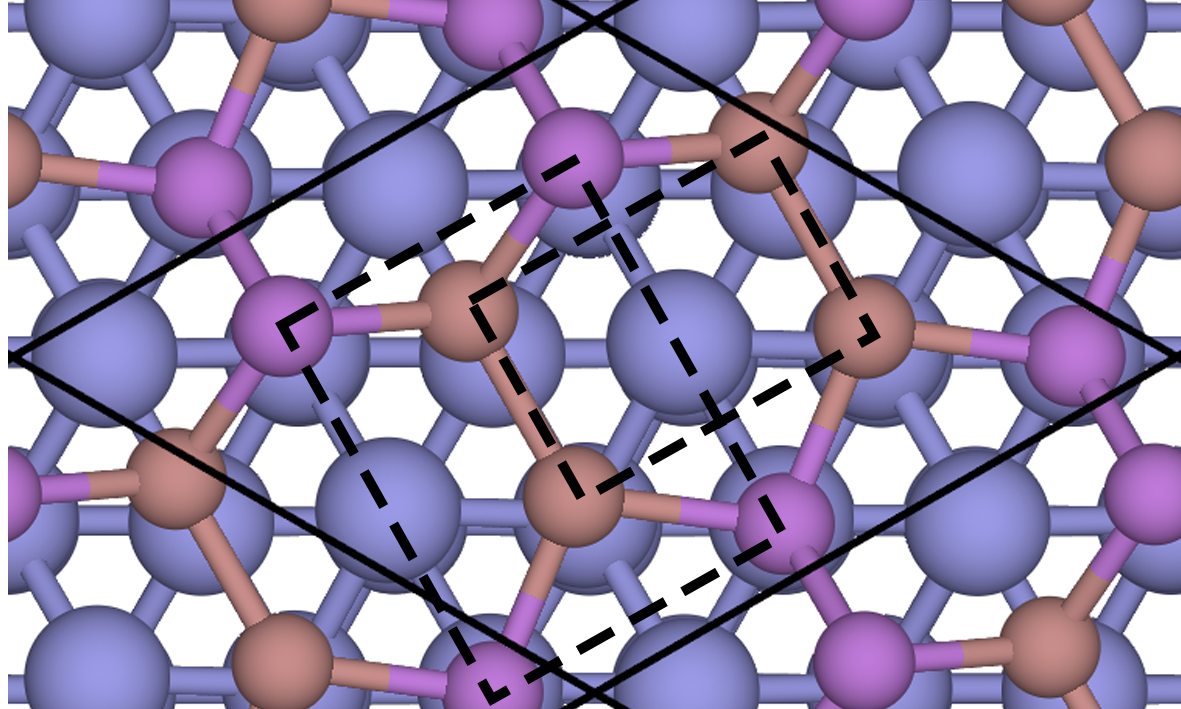
\includegraphics[width=0.28\textwidth]{pic/IS_structure_1Linsb_22rectop.png}
        \end{tabular}
    }\\[-1ex]
    \subfloat[]{
        \label{fig:IS_structure_1Linsb_22str}
        \begin{tabular}{c}
            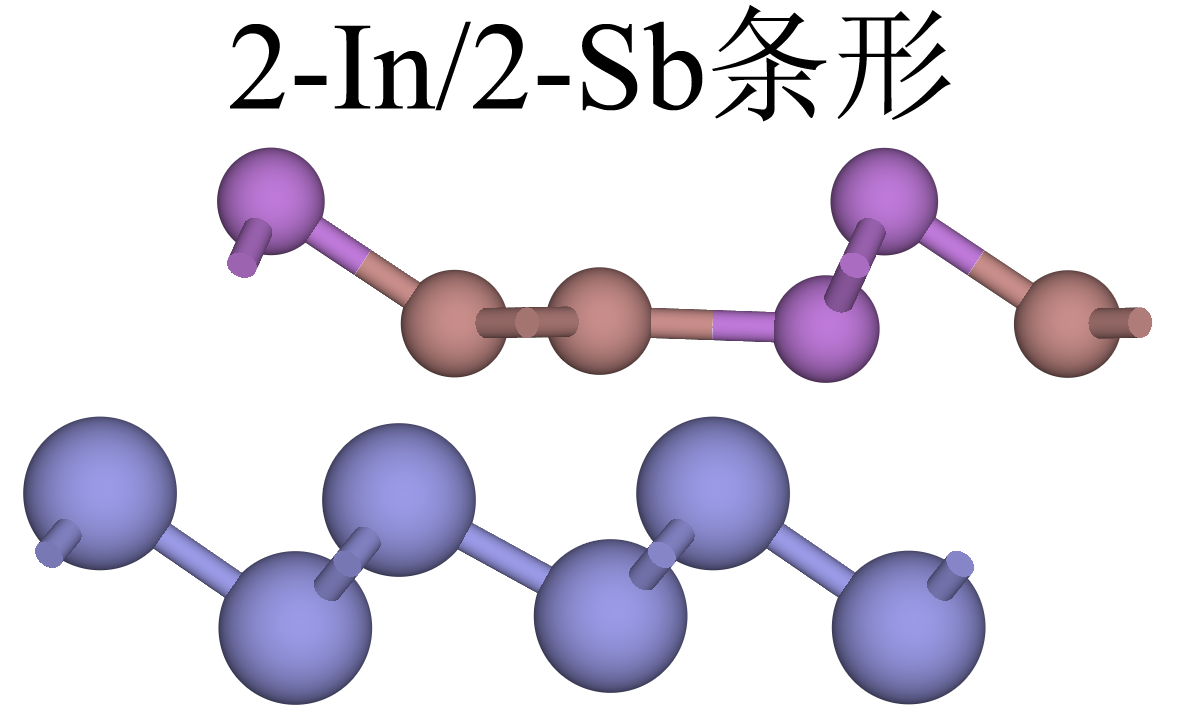
\includegraphics[width=0.28\textwidth]{pic/IS_structure_1Linsb_22strside.png} \\
            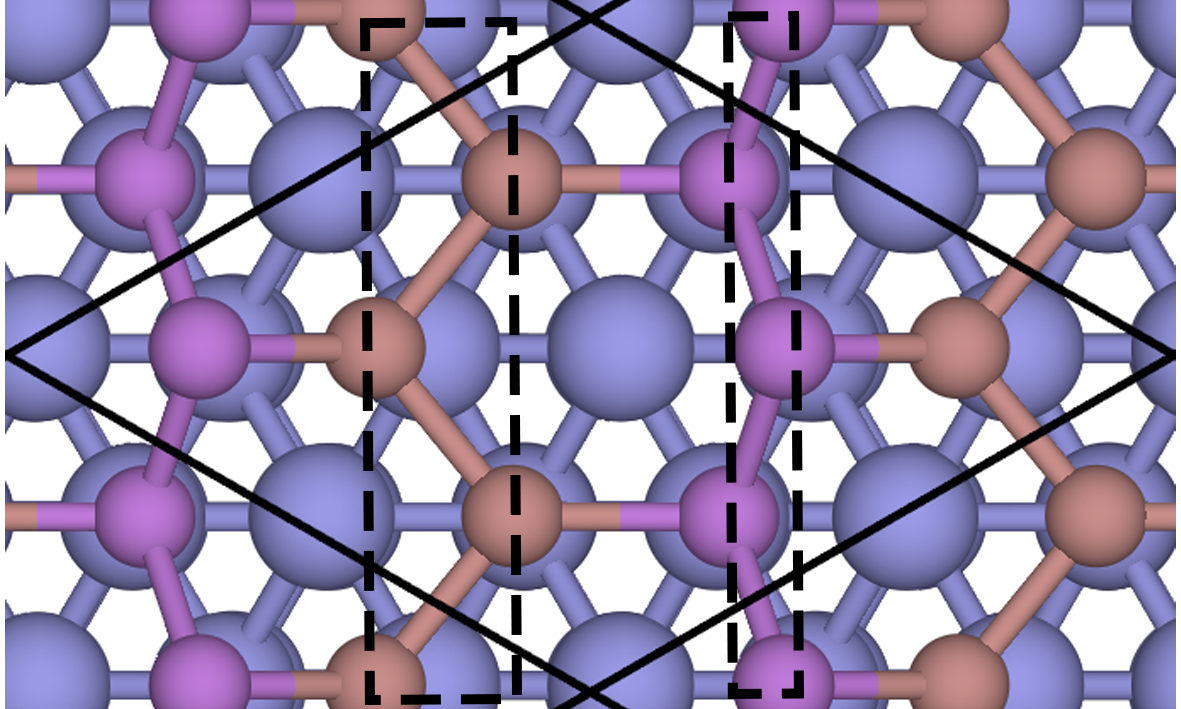
\includegraphics[width=0.28\textwidth]{pic/IS_structure_1Linsb_22strtop.png}
        \end{tabular}
    }
    \subfloat[]{
        \label{fig:IS_structure_1Linsb_31}
        \begin{tabular}{c}
            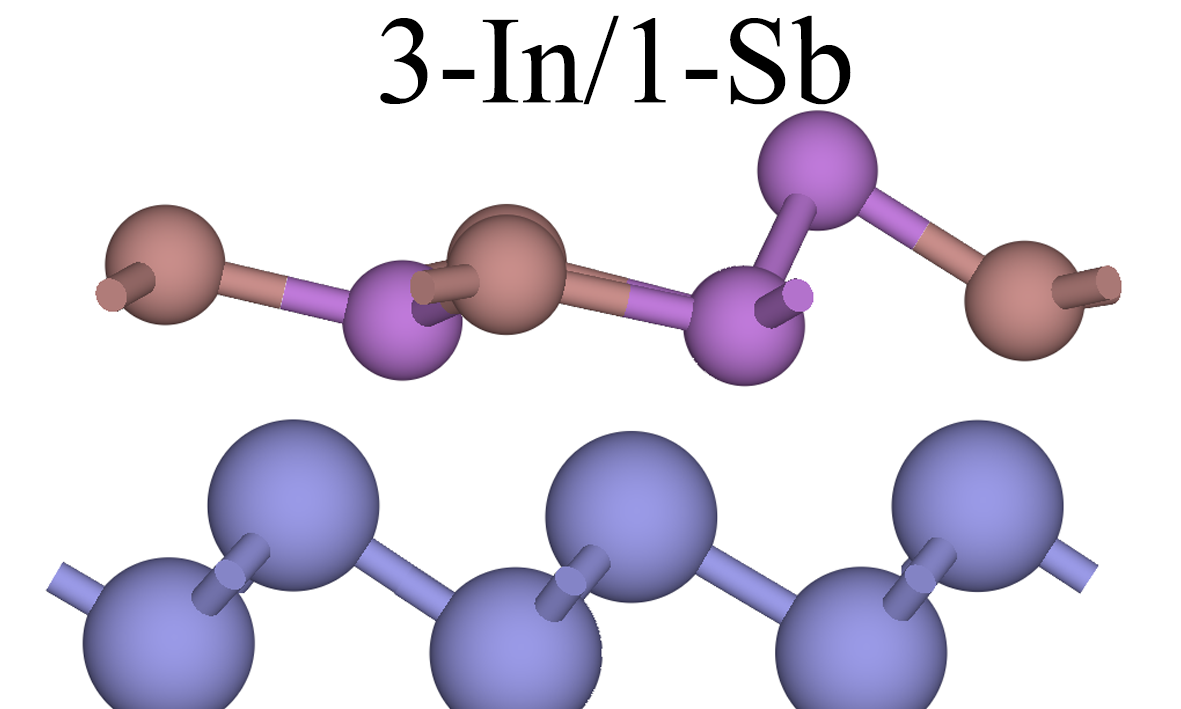
\includegraphics[width=0.28\textwidth]{pic/IS_structure_1Linsb_31side.png} \\
            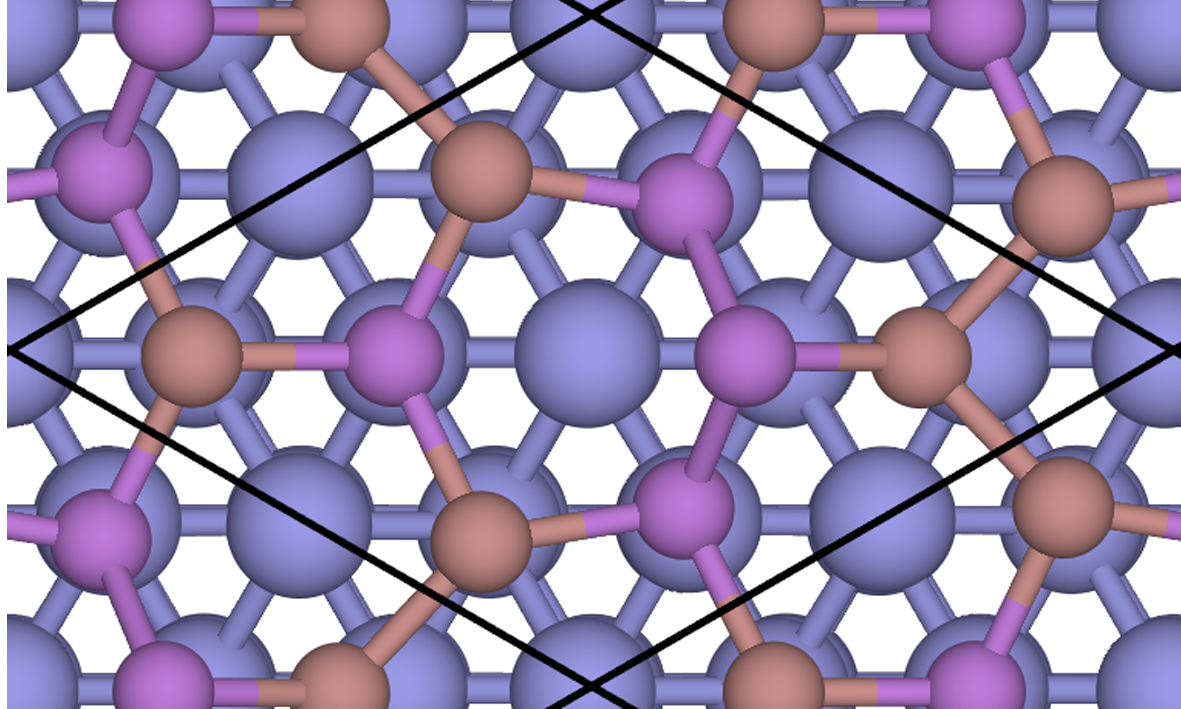
\includegraphics[width=0.28\textwidth]{pic/IS_structure_1Linsb_31top.png}
        \end{tabular}
    }
    \subfloat[]{
        \label{fig:IS_structure_1Linsb_40}
        \begin{tabular}{c}
            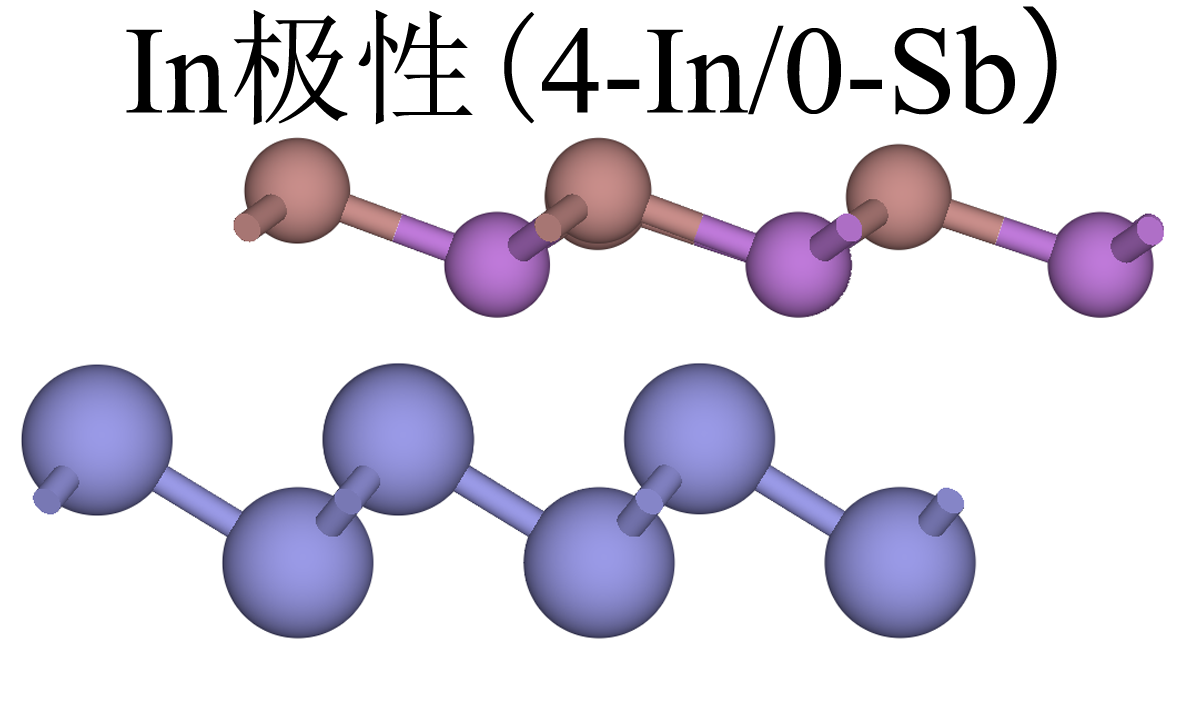
\includegraphics[width=0.28\textwidth]{pic/IS_structure_1Linsb_40side.png} \\
            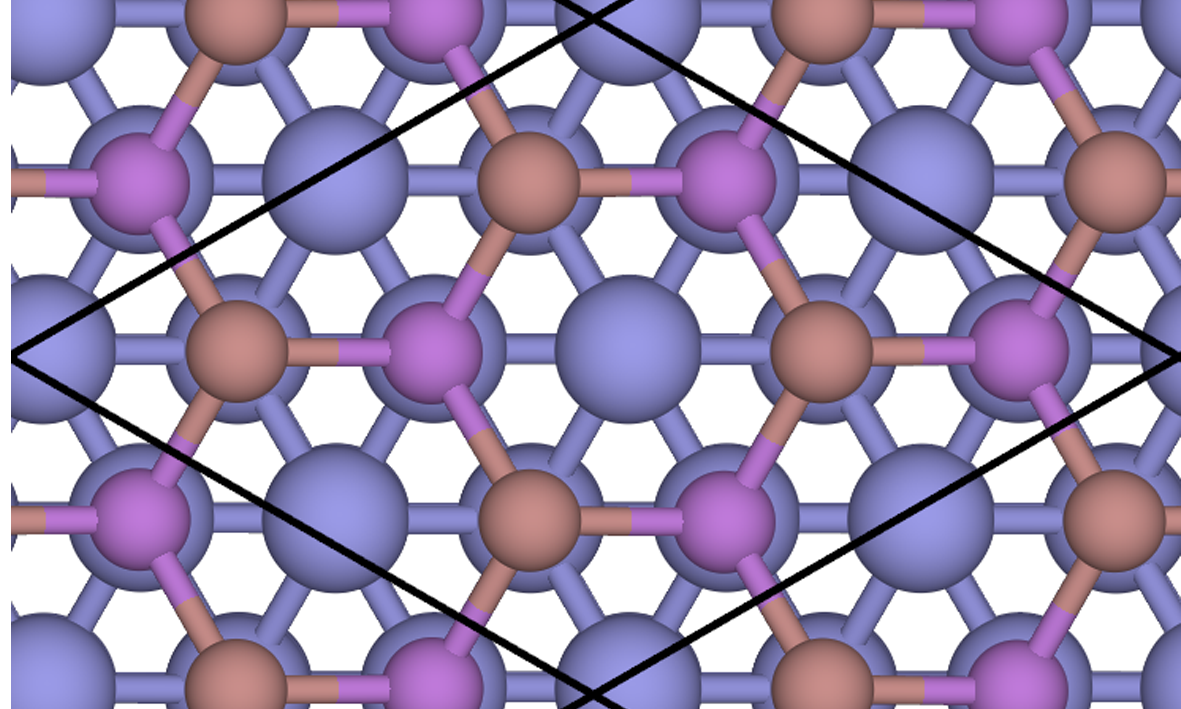
\includegraphics[width=0.28\textwidth]{pic/IS_structure_1Linsb_40top.png}
        \end{tabular}
    }
    \caption{\cemb{Bi(001)}衬底上不同极性单层\cemb{InSb}的原子结构。原子结构图中,\cemb{Bi}原子使用蓝色表示,\cemb{In}原子使用褐色表示,\cemb{Sb}原子使用紫色表示。}
    \label{fig:IS_structure_1Linsb_allPolarity}
\end{figure}

接着,我们将单层\cemb{InSb(111)}极性的考察范围扩大到非理想的情况。考虑到吸附的\cemb{In}原子和\cemb{Sb}原子均倾向于沉积在$\TfourSite$位点和$\HthreeSite$位点,使用包含四个\cemb{In}原子和四个\cemb{Sb}原子的$2 \times 2$切片模型,我们可以列举出六种可能的单层\cemb{InSb}极性。在图\ref{fig:IS_structure_1Linsb_allPolarity}中,我们列出了本章中所考虑的所有单层\cemb{InSb}的极性情况。这里,我们使用\cemb{InSb}单层中处于$\TfourSite$的原子的数量来表示不同极性的\cemb{InSb(111)}单层,例如在$2 \times 2$切片模型中理想的\cemb{In}极性\cemb{InSb}中,四个$\TfourSite$都被\cemb{In}原子占据,因此可以表示为$\InSbMLpolar{4}{0}$。相对应的,\cemb{Sb}极性的\cemb{InSb}可以表示为$\InSbMLpolar{0}{4}$。对于$\InSbMLpolar{2}{2}$极性的\cemb{InSb}单层,有两个不等价的构型。其中一个构型内部\cemb{In}原子和\cemb{Sb}分别构成两个相互嵌套的方形的四个顶角,我们用$\InSbMLpolar{2}{2}$方形表示。另一个构型中\cemb{In}原子和\cemb{Sb}原子呈条状分布,我们用$\InSbMLpolar{2}{2}$条形表示。


如图\ref{fig:IS_DFT_1LInSb_all}所示,我们计算了所有极性的$2 \times 2 \cemb{InSb}$在\cemb{Bi(001)}衬底表面的形成能。在$2 \times 2$模型中,\cemb{In}极性($\InSbMLpolar{4}{0}$)的形成能为\SI{-18.52}{\mievpas},低于$2 \times 2$模型中\cemb{Sb}极性($\InSbMLpolar{0}{4}$)的形成能(\SI{-14.64}{\mievpas})。$2 \times 2 \cemb{InSb}$理想极性(\cemb{Sb}极性和\cemb{In}极性)的计算结果与上一节中$1 \times 1$模型一致。$2 \times 2$模型中更低的形成能可能是由于表面原子在$2 \times 2$模型中有更多的空间可以进行更完全的几何优化。


\begin{figure}[htb]
    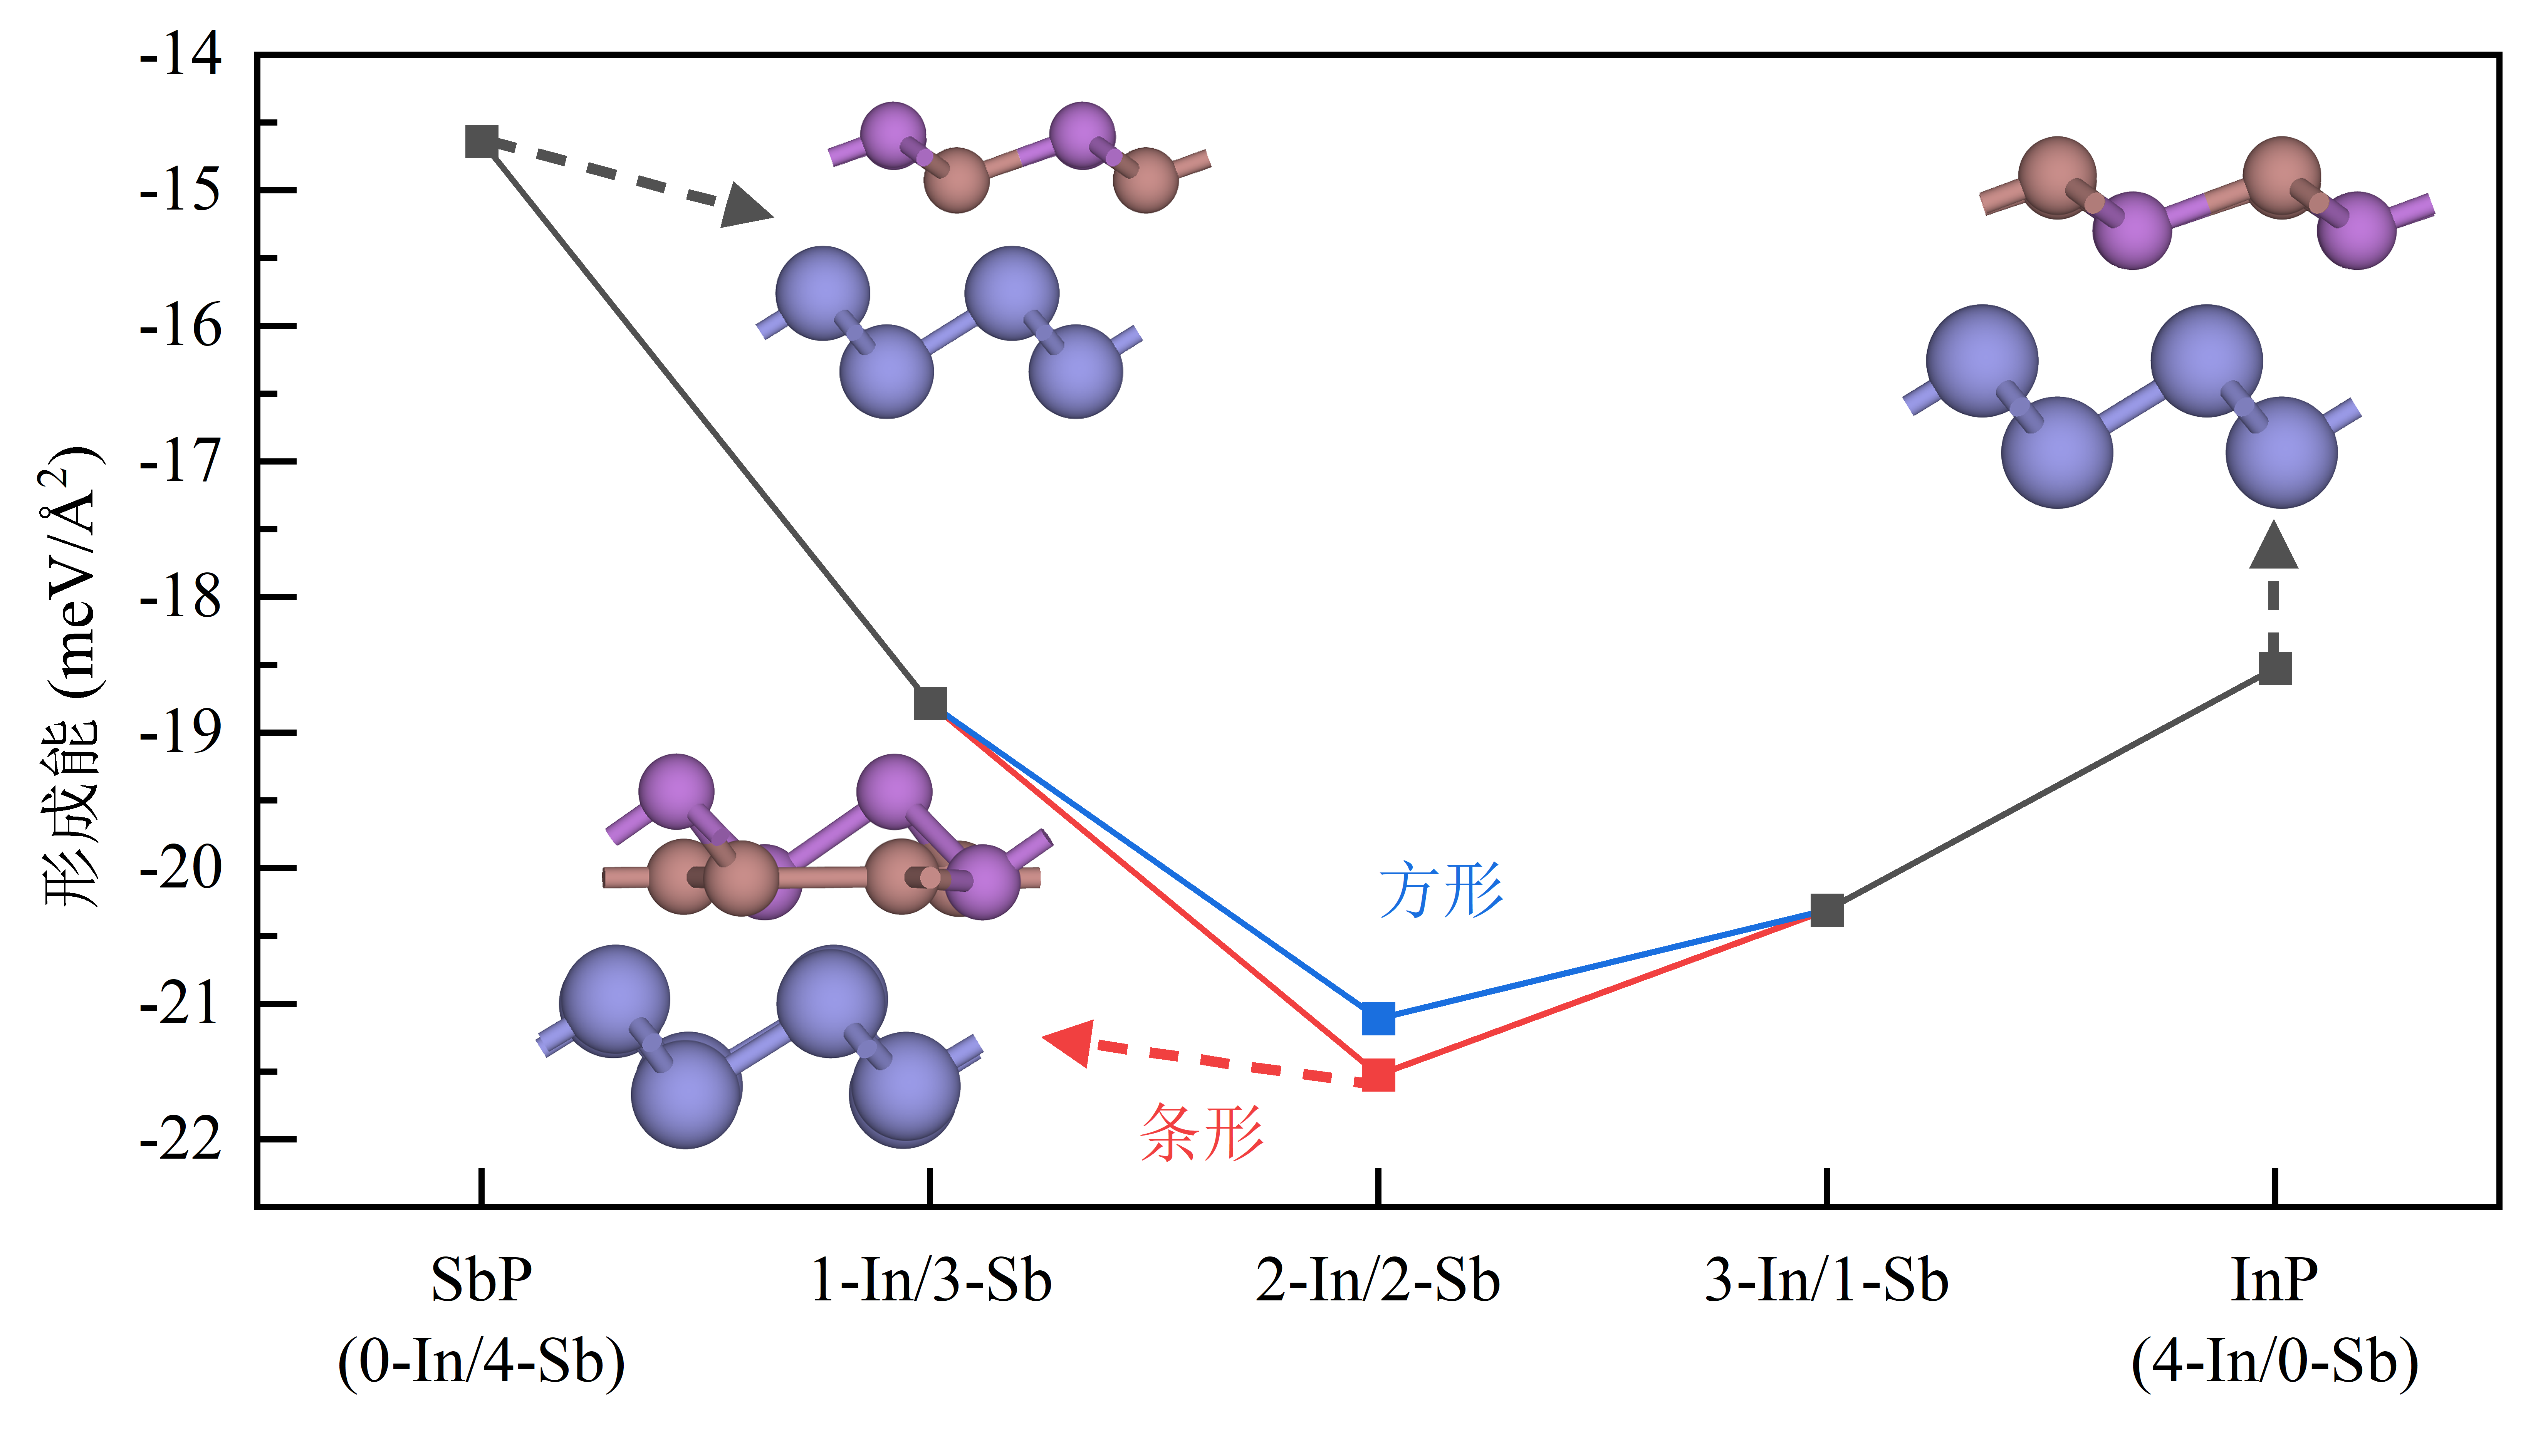
\includegraphics{pic/IS_DFT_1LInSb_all.png}
    \caption{\cemb{Bi(001)}衬底上不同极性单层\cemb{InSb}的形成能。}
    \label{fig:IS_DFT_1LInSb_all}
\end{figure}

在我们的进一步计算中,我们发现混合极性的单层\cemb{InSb(111)}构型(\InSbMLpolar{1}{3}、\InSbMLpolar{2}{2}以及\InSbMLpolar{3}{1})在形成能上更具有优势。从图\ref{fig:IS_DFT_1LInSb_all}上可以看出,混合极性中能量最低的\InSbMLpolar{1}{3}构型的形成能也略低于理想极性中更为稳定的\cemb{In}极性(\InSbMLpolar{4}{0})。因此,由于混合极性具有更高的能量稳定性,在生长的过程中\cemb{InSb}单层会倾向于由理想极性的结构(\cemb{Sb}极性和\cemb{In}极性)转变为混合极性。在4种混合极性中$\InSbMLpolar{2}{2}$结构的单层\cemb{InSb}的形成能最低。其中,$\InSbMLpolar{2}{2}$ 条形构型的形成能略低与$\InSbMLpolar{2}{2}$方形构型的形成能。这两形成能相近的$\InSbMLpolar{2}{2}$构型形成的能量最低态使得混合极性的\cemb{InSb}单层倾向于较为均匀的分布于这两个$\InSbMLpolar{2}{2}$构型之中,形成类似于非晶态的\cemb{InSb}单层。

利用分子动力学模拟方法,我们测试了$\InSbMLpolar{2}{2}$构型的热稳定性。如图\ref{fig:IS_structure_1Linsb_md}所示,我们选用形成能更低的$\InSbMLpolar{2}{2}$ 条形构型作为考察对象(图\ref{fig:IS_structure_1Linsb_md0ps}),模拟温度设为生长\cemb{InSb}常见的\SI{400}{\kelvin}。可能看到,在经过\SI{30}{\pico\second}的分子动力学模拟后。\cemb{InSb}单层的晶格结构被略微破坏,其中\cemb{In}的条状构型已经被热动能破坏,形成类似于菱形的结构,而\cemb{Sb}的条状构型保持较为完好。综合以上的计算结果,我们认为\cemb{InSb(111)}单层在\cemb{Sb(001)}衬底上由于热涨落的作用很可能无法保持在唯一的构型下,而是处于不同混合极性的热平衡态。在热平衡中,不同极性的\cemb{InSb}在热动能的驱动下相互转化,形成非晶态的单层\cemb{InSb}形貌。

\begin{figure}[!htb]
    \subfloat[]{
        \label{fig:IS_structure_1Linsb_md0ps}
        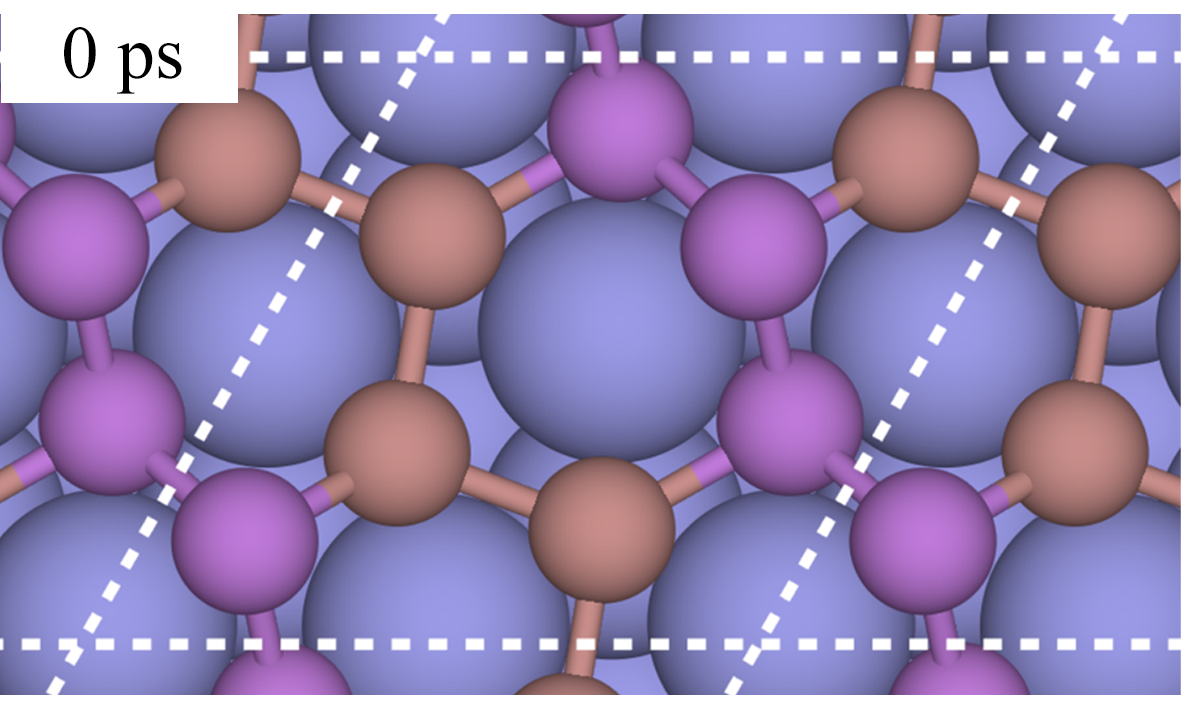
\includegraphics{pic/IS_structure_1Linsb_md0ps.png}
    }
    \subfloat[]{
        \label{fig:IS_structure_1Linsb_md10ps}
        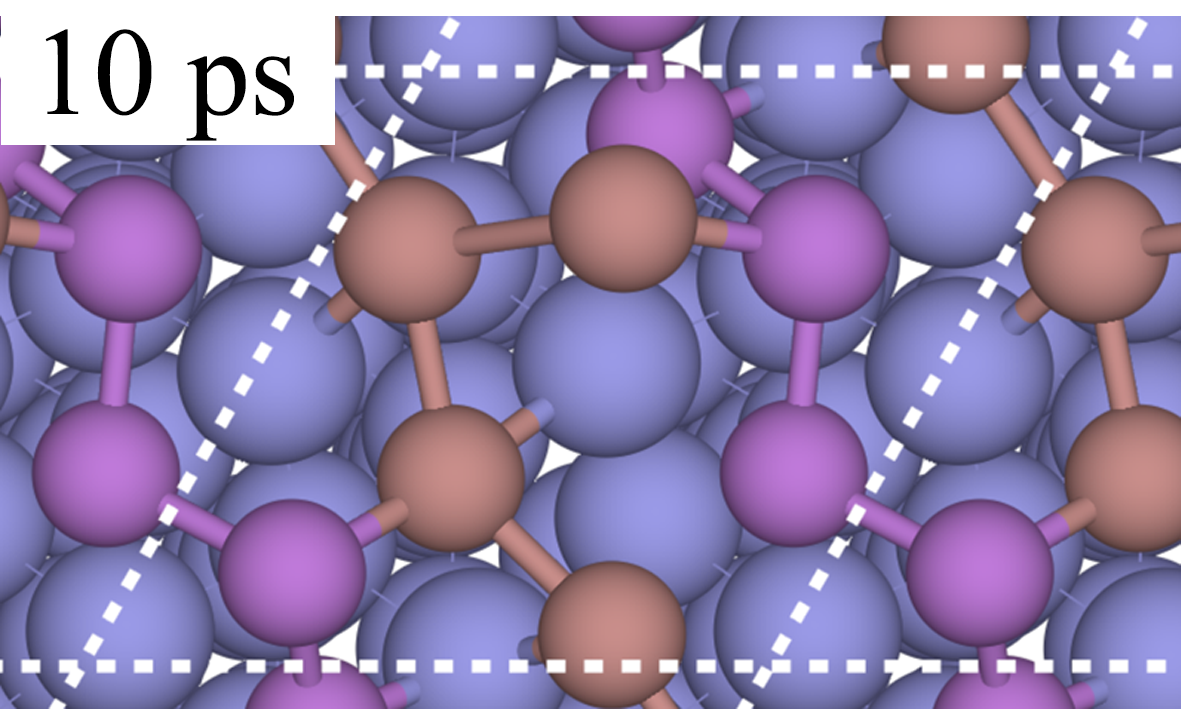
\includegraphics{pic/IS_structure_1Linsb_md10ps.png}
    }\\[-1ex]

    \subfloat[]{
        \label{fig:IS_structure_1Linsb_md20ps}
        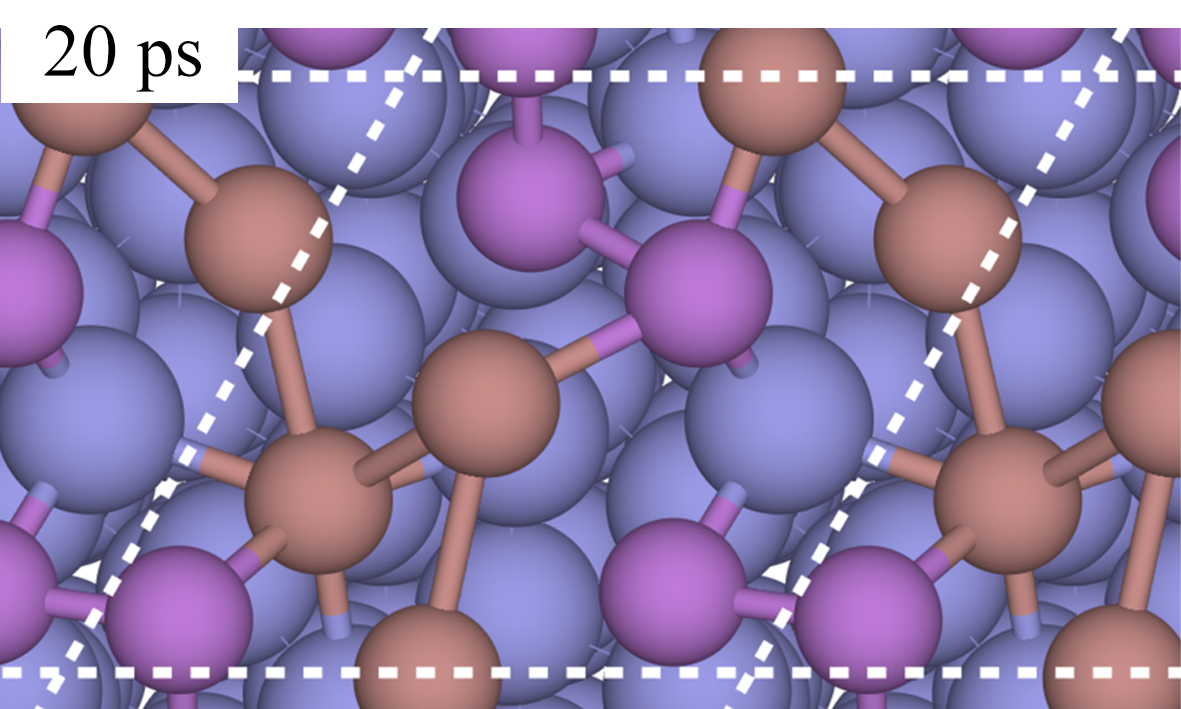
\includegraphics{pic/IS_structure_1Linsb_md20ps.png}
    }
    \subfloat[]{
        \label{fig:IS_structure_1Linsb_md30ps}
        \includegraphics{pic/IS_structure_1Linsb_md30ps.png}
    }
    \caption{\cemb{Bi(001)}衬底上2-In/2-Sb条形极性\cemb{InSb}的分子动力学模拟结果。原子结构图中,\cemb{Bi}原子使用蓝色表示,\cemb{In}原子使用褐色表示,\cemb{Sb}原子使用紫色表示。}
    \label{fig:IS_structure_1Linsb_md}
\end{figure}

单层\cemb{InSb(111)}不同极性之间的转换能力我们通过将单层\cemb{InSb(111)}由一个极性的构型转变为另一个极性的构型所需的势垒进行判定。取\cemb{Sb}极性和\cemb{In}极性的的\cemb{InSb}单层之间的转换作为代表。这两个极性之间的转变涉及\cemb{InSb}单层内部所有的\cemb{In}原子和\cemb{Sb}原子,因此我们将其作为\cemb{InSb}极性转换势垒的上界。过渡态的计算结果如图\ref{fig:IS_DFT_1LInSb_InPtoSbPNeb}所示,从能量更高的\cemb{Sb}极性结构转变到\cemb{In}极性,单层\cemb{InSb}需要跨越约\SI{0.60}{\electronvolt}的势垒。根据统计力学原理\citing{RN945-1935},单层\cemb{InSb}从\cemb{Sb}极性转变到\cemb{In}极性的频率$r$为\chinesecolon
\[
    r=e^{\frac{-\energyVar{a}{}}{\kbconst T}}e^{\frac{\Delta S}{\kbconst}} \frac{\kbconst T}{h}
\]

其中,$\energyVar{a}{}$为反应的激活能,$\kbconst$为玻尔兹曼常数,$T$为温度,$h$为普朗克常数,$\Delta S$为反应过程中初态和过渡态之间的熵变,我们使用密度泛函理论计算结合原子震动能谱分析进行计算。在\SI{400}{\kelvin}的温度下,单层\cemb{InSb}从\cemb{Sb}极性转变到\cemb{In}极性的频率$r$约为\SI{3e5}{\per\second},证明了在\cemb{Bi(001)}衬底表面,\cemb{InSb}单层具有较高的极性转变能力。

\begin{figure}[!htb]
    \includegraphics{pic/IS_DFT_1InSb_flipBarrier.png}
    \caption{\cemb{Bi(001)}衬底上单层\cemb{InSb}的极性转换势垒。原子结构图中,\cemb{Bi}原子使用蓝色表示,\cemb{In}原子使用褐色表示,\cemb{Sb}原子使用紫色表示。}
    \label{fig:IS_DFT_1LInSb_InPtoSbPNeb}
\end{figure}

\section{双层锑化铟的生长机理}
在上一节中,我们通过理论计算表明了单层的\cemb{InS(111)}以$\InSbMLpolar{2}{2}$极性为主,多种极性热平衡混合的构型存在于\cemb{Bi(001)}衬底的表面。我们将第二层\cemb{InSb(001)}放置在单层\cemb{InSb}上方,研究双层\cemb{InSb(111)}在\cemb{Bi(001)}衬底上的生长机理和极性演化情况。

\subsection{双层锑化铟的生长过程}
对于双层\cemb{InSb}在\cemb{Bi(001)}衬底上的生长,我们首先探究第二层\cemb{InSb(111)}对于\cemb{InSb}极性的影响。对于第二层\cemb{InSb(111)},我们选用对应的表面重构构型进行代表。根据先前的研究\citing{RN915-1998, RN896-1998},在\cemb{InSb(111)}的表面由于极性的不同会形成两种不同的表面重构,一种是对应于\cemb{Sb}极性的\cemb{Sb}三聚体(\cemb{Sb} trimer)表面重构,另一种是对应于\cemb{In}极性的\cemb{In}空位(\cemb{In} vacancy)表面重构。

如图\ref{fig:IS_structure_2Linsb}所示,我们考虑不同表面重构的\cemb{InSb}第二层和不同极性的\cemb{InSb}第一层的所有组合进行形成能计算。以\cemb{In}极性的\cemb{InSb}第一层为代表,我们在图\ref{fig:IS_structure_2Linsb_SbT40}和图\ref{fig:IS_structure_2Linsb_InV40}中绘制了优化后的双层\cemb{InSb}的原子结构。可以看到对于\cemb{Sb}三聚体的第二层能够与\cemb{In}极性的第一层的上表面\cemb{In}原子产生相互作用,略微提高于其相接触的\cemb{In}原子的相对高度。对于\cemb{In} 空位的第二层,其在\cemb{In}极性的第一层\cemb{InSb}上方呈现出平面化的形貌。\cemb{In}空位重构中四个\cemb{Sb}原子与第一层上表面的\cemb{In}原子产生作用。

\begin{figure}[!htb]
    \subfloat[]{
        \label{fig:IS_2LInSb_config}
        \includegraphics[width=0.48\textwidth]{pic/IS_2LInSb_config.pdf}
    }
    \begin{minipage}[b]{0.5\textwidth}
        \subfloat[]{
            \label{fig:IS_structure_2Linsb_SbT40}
            \includegraphics[width=0.8\textwidth]{pic/IS_structure_2Linsb_SbT-40_3Dview.png}
        }
        \newline
        \subfloat[]{
            \label{fig:IS_structure_2Linsb_InV40}
            \includegraphics[width=0.8\textwidth]{pic/IS_structure_2Linsb_InV-40_3Dview.png}
        }
    \end{minipage}
    \caption{双层\cemb{InSb}极性极性组合图及原子结构示意图。(a)双层\cemb{InSb}极性极性组合示意图;(b)双层\cemb{InSb}原子结构,\cemb{Sb}三聚体第二层覆盖\cemb{In}极性第一层;(b)双层\cemb{InSb}原子结构,\cemb{In}空位第二层覆盖\cemb{In}极性第一层。原子结构图中,\cemb{Bi}原子使用蓝色表示,\cemb{In}原子使用褐色表示,\cemb{Sb}原子使用紫色表示。}
    \label{fig:IS_structure_2Linsb}
\end{figure}

在图\ref{fig:IS_DFT_2LInSb_formationEnergy}中,我们绘制了\cemb{Bi(001)}衬底上具有不同极性第一层\cemb{InSb}的双层\cemb{InSb}的形成能分布。先前的研究表明,不同的前驱体比例会对生长形貌产生极大的影响\citing{RN935-2002, RN398-2002}。因此同\cemb{In}和\cemb{Sb}原子的吸附机制研究一致,我们引入\cemb{In}原子的化学势$\muVar{In}{}$代表生长环境中$\cemb{In}:\cemb{Sb}$比的变化。为了绘图清晰,我们在图\ref{fig:IS_DFT_2LInSb_formationEnergy}只绘制了不同构型在纯\cemb{Sb}环境和纯\cemb{In}环境两个极限下的形成能取值。由于在\cemb{Sb}三聚体重构和\cemb{In}空位重构中,均为\cemb{Sb}原子的数量占有,因此根据式\ref{eq:IS_formationEnenrgy}和式\ref{eq:IS_bulkEqmb},以\cemb{Sb}三聚体重构和\cemb{In}空位重构为第二层的双层\cemb{InSb}的形成能均会随着\cemb{In}原子化学式$\muVar{In}{}$的上升(接近纯\cemb{In}环境)而上升。

\begin{figure}[!htb]
    \subfloat[]{
        \includegraphics[width=0.45\textwidth]{pic/IS_DFT_2LInSb_SbTonAll.png}
        \label{fig:IS_DFT_2LInSb_SbTonAll}
    }
    \subfloat[]{
        \includegraphics[width=0.45\textwidth]{pic/IS_DFT_2LInSb_InVonAll.png}
        \label{fig:IS_DFT_2LInSb_InVonAll}
    }
    \caption{\cemb{Bi(001)}衬底上双层\cemb{InSb}的形成能分布。(a)以Sb三聚体为第二层的双层\cemb{InSb}的形成能分布;(b)以In空位层为第二层的双层\cemb{InSb}的形成能分布。}
    \label{fig:IS_DFT_2LInSb_formationEnergy}
\end{figure}

当第二层为\cemb{Sb}三聚体重构时,第一层为理想极化结构(\cemb{Sb}极性和\cemb{In}极性)的双层\cemb{InSb}相比于第一层为混合极化结构的双层\cemb{InSb}拥有更低的形成能。理想极化的第一层\cemb{InSb}在形成能分布中作为两个极小值点,吸引其他拥有混合极性第一层的双层\cemb{InSb}向理想极化转变。使得原本在非静态单层中以混合极性为主的平衡态分化成为\cemb{Sb}极性和\cemb{In}极性共存的多晶态。同时,当生长环境中的接近纯\cemb{In}极限时,第一层为混合极性的双层\cemb{InSb}的形成能大于零而第一层为理想极性的双层\cemb{InSb}的形成能保持在小于零的状态。在这种情况下,由于较高的\cemb{In}原子活性,可能会导致第一层为混合极性的双层\cemb{InSb}分解,进一步加速了双层\cemb{InSb}向理想极性的第一层构型转化。

当第二层为\cemb{In}空位重构时,\cemb{In}空位层和作为第一层的\cemb{Sb}极性\cemb{InSb}之间的作用没有\cemb{Sb}三聚体作为第二层时的那么强烈。\cemb{In}空位重构的第二层无法\cemb{Sb}极性的第一层的形成能降低到混合极性之下。导致了第二层为\cemb{In}空位重构时,在双层\cemb{InSb}中只有第一层为\cemb{In}极性时为最小能量态。在\cemb{In}空位重构下,\cemb{Sb}极性的第一层只需要跨越\SI{0.63}{\mievpas}的能量台阶(\InSbMLpolar{1}{3})即可一步步翻转至\cemb{In}极性的第一层,其中的过程均为放热反应。在这种情况下,我们认为当第二层为\cemb{In}空位重构时,极性为混合极性或者\cemb{Sb}极性的第一层会逐渐极化至\cemb{In}极性。

在图\ref{fig:IS_DFT_2LInSb_formationEnergy}中,形成能的计算显示在生长了第二层\cemb{InSb}后,重构的第二层\cemb{InSb}会使得第一层已生长的非晶态\cemb{InSb}趋向于转变为多晶的形态(第二层为\cemb{Sb}三聚体重构)或者\cemb{In}极性的形态(第二层为\cemb{In}空位重构)。

为了探究在双层\cemb{InSb}中第一层\cemb{InSb}由非晶态向单一\cemb{In}极性转变的动力学过程,我们以\cemb{In}空位作为第二层,$\InSbMLpolar{2}{2}$条形构型作为第一层组成的双层\cemb{InSb}作为研究对象,在\cemb{Bi}衬底上进行分子动力学模拟。如图\ref{fig:IS_structure_2Linsb_md50ps}所示,在经过了\SI{50}{\pico\second}的分子动力学模拟后,可以看到第一层的$\InSbMLpolar{2}{2}$构型已经完全被破坏。有一个原属于第一层的\cemb{Sb}原子越过一二层\cemb{InSb}的界面,被挤入了第二层。同时,第一层的\cemb{InSb}由于缺少了一个\cemb{Sb}原子,原本晶格中的褶皱变得扁平。随着分子动力学模拟的继续,第一个\cemb{In}极性的次表面出现在模拟开始约\SI{60}{\pico\second}的时候(图\ref{fig:IS_structure_2Linsb_md60ps})。这个次表面是一个位于顶点的\cemb{In}原子和三个位于底部的\cemb{Sb}原子组成的四面体结构,并且在我们的模拟过程中一直维持到了\SI{100}{\pico\second}(图\ref{fig:IS_structure_2Linsb_md100ps})。

\begin{figure}[!htb]
    \subfloat[]{
        \includegraphics[width=0.4\textwidth]{pic/IS_structure_2Linsb_md50ps.png}
        \label{fig:IS_structure_2Linsb_md50ps}
    }
    \subfloat[]{
        \includegraphics[width=0.4\textwidth]{pic/IS_structure_2Linsb_md60ps.png}
        \label{fig:IS_structure_2Linsb_md60ps}
    }\\[-0.5ex]
    \subfloat[]{
        \includegraphics[width=0.4\textwidth]{pic/IS_structure_2Linsb_md100ps.png}
        \label{fig:IS_structure_2Linsb_md100ps}
    }
    \subfloat[]{
        \includegraphics[width=0.4\textwidth]{pic/IS_structure_2Linsb_md100psopt.png}
        \label{fig:IS_structure_2Linsb_md100psopt}
    }
    \caption{\cemb{Bi(001)}衬底上双层\cemb{InSb}极性演化的分子动力学模拟结果。(a)分子动力学模拟50ps后的原子结构图;(b)分b动力学模拟60ps后的原子结构图;(c)分子动力学模拟100ps后的原子结构图;(d)100ps对应中间态的原子结构图。原子结构图中,\cemb{Bi}原子使用蓝色表示,\cemb{In}原子使用褐色表示,\cemb{Sb}原子使用紫色表示。}
    \label{fig:IS_structure_2Linsb_md}
\end{figure}

由于计算能力和模拟时长的限制,我们未能在模拟的时限内发现\cemb{In}空位重构层下第一层\cemb{InSb}完全转变为\cemb{In}极化构型。我们对进行了分子动力学模拟\SI{100}{\pico\second}后的双层\cemb{InSb}模型进行了结构优化,以去除分子动力学模拟中的热扰动热扰动,获得在热动能的驱动下,双层\cemb{InSb}极性演化的中间态。如图\ref{fig:IS_structure_2Linsb_md100psopt}所示,在经过结构优化后,双层\cemb{InSb}极性演化的中间态具有两个\cemb{In}次表面四面体,显示出半\cemb{In}极化的结构。同时,形成能的计算显示这个双层\cemb{InSb}极性演化的中间态的形成能介于\cemb{In}极性的第一层和$\InSbMLpolar{2}{2}$的第一层之间。进一步印证了在热动能的驱使下,双层\cemb{InSb}会逐渐从原本以混合极性为主的非晶态慢慢极化至\cemb{In}极性。

\begin{figure}[!htb]
    \subfloat[]{
        \includegraphics{pic/IS_DFT_2InSb_adatoms.png}
    }\\[-0.5ex]
    \subfloat[]{
        \includegraphics{pic/IS_structure_2Linsb_adatoms_InT4.png}
    }
    \subfloat[]{
        \includegraphics{pic/IS_structure_2Linsb_adatoms_InH3.png}
    }\\[-0.5ex]
    \subfloat[]{
        \includegraphics{pic/IS_structure_2Linsb_adatoms_SbT4.png}
    }
    \subfloat[]{
        \includegraphics{pic/IS_structure_2Linsb_adatoms_SbH3.png}
    }
    \caption{\cemb{In}原子和\cemb{Sb}原子在\InSbMLpolar{2}{2}条形单层\cemb{InSb}表面吸附的结合能和吸附原子结构图。(a)吸附原子结合能;(b)\cemb{In}原子吸附在$\TfourSite$位;(c)\cemb{Sb}原子吸附在$\HthreeSite$位;(d)\cemb{In}原子吸附在$\TfourSite$位;(e)\cemb{Sb}原子吸附在$\HthreeSite$位。原子结构图中,\cemb{Bi}原子使用蓝色表示,\cemb{In}原子使用褐色表示,\cemb{Sb}原子使用紫色表示。}
    \label{fig:IS_2Linsb_adatom}
\end{figure}


为了揭示双层\cemb{InSb}的极化过程,我们首先对第二层\cemb{InSb}的生长过程进行探究。与在\cemb{Bi(001)}表面生长单层\cemb{InSb}类似,我们计算了\cemb{In}和\cemb{Sb}原子在单层\cemb{InSb}表面的吸附过程。考虑单层\cemb{InSb}以混合极性为主的非静态构型以及不同极性的形成能高低(图\ref{fig:IS_DFT_1LInSb_all}),我们选用$\InSbMLpolar{2}{2}$条形结构的单层\cemb{InSb}作为吸附表面。如图\ref{fig:IS_2Linsb_adatom}所示,我们同样考虑单层\cemb{InSb}表面$\TfourSite$位点和$\HthreeSite$位点对于\cemb{In}和\cemb{Sb}原子的吸附能力。与在\cemb{Bi}表面吸附不同,单层\cemb{InSb}对于\cemb{In}原子的吸附能力弱于\cemb{Sb}原子。在各自的浓度比例极限中,\cemb{Sb}原子吸附在\cemb{InSb}表面具有比\cemb{In}原子更高的结合能。同时,\cemb{Sb}原子与单层\cemb{InSb}更强的相互作用使得\cemb{Sb}原子吸附的为放热反应的$\muVar{In}{}$范围宽于\cemb{In}原子。对于\cemb{Sb}原子而言,其可以在生长环境中\cemb{In}原子浓度略高的情况下在单层\cemb{InSb}的表面吸附($\muVar{In}{}\leqslant \SI{-2.70}{\electronvolt}$)。而\cemb{In}原子只能在$\muVar{In}{} \geqslant \SI{-2.68}{\electronvolt}$的生长环境下才倾向于在单层的\cemb{InSb}表面吸附。在$\InSbMLpolar{2}{2}$条形结构的\cemb{InSb}的表面,没有能够同时吸附\cemb{In}原子和\cemb{Sb}原子的$\muVar{In}{}$窗口。因此,在第二层\cemb{InSb}成核生长的早期,由于生长环境中原子比例和化学活性的不同,在\cemb{In}和\cemb{Sb}之间只有一种原子能够直接在单层\cemb{InSb}表面吸附。我们可以通过调节生长环境中的浓度比例调控在单层\cemb{InSb}的优先吸附原子类型。

\begin{figure}[!htb]
    \subfloat[]{
        \includegraphics{pic/IS_structure_InxSb3-x_A.png}
    }
    \subfloat[]{
        \includegraphics{pic/IS_structure_InxSb3-x_B.png}
    }
    \caption{单层\cemb{InSb}表面生长团簇(\cemb{In_xSb_{3-x}})的构型。(a)A类\cemb{In_xSb_{3-x}}团簇的原子构型;(b)B类\cemb{In_xSb_{3-x}}团簇的原子构型}
    \label{fig:IS_structure_InxSb3-x}
\end{figure} 

随着生长的进行,原本难以在单层\cemb{InSb}表面吸附的原子可能和已吸附的原子成键,形成团簇。团簇的生长形态和化学组成同样可能受到生长环境中$\muVar{In}{}$变化的影响。考虑第二层为到\cemb{Sb}三聚体重构时,于双层\cemb{InSb}的形成能谱(图\ref{fig:IS_DFT_2LInSb_SbTonAll})可以认为第一层混合极性的\cemb{InSb}的晶体化转变开始于作为第二层的\cemb{Sb}团簇重构层将第一层引导至理想极性的构型(\cemb{In}极性或者\cemb{Sb}极性)。同时,我们注意到从原子结构的角度看,\cemb{In}空位重构的原子结构可以由\cemb{Sb}三聚体重构表面继续吸附三个\cemb{In}原子和一个\cemb{Sb}原子形成。因此,在生长的过程中,\cemb{In}重构表面的第二层可能是从团簇阶段的\cemb{Sb}三聚体重构表面演化而来,并在\cemb{Sb}三聚体重构的第二层基础上进一步将第一层多晶态的\cemb{InSb}完全极化至\cemb{In}极性。

在生长过程的团簇阶段,我们需要验证\cemb{Sb}三聚体是否是生长过程中最为可能的团簇形态。因此,我们进一步考察了团簇生长阶段不同形貌的三聚体在\cemb{InSb}自极化过程中的形貌以及作为第二层的\cemb{InSb}团簇在不同$\muVar{In}{}$环境下的演化规律。通过先前的计算,我们已经得知作为第二层的\cemb{Sb}三聚体重构可以将原本极性混乱的第一层\cemb{InSb}引导至\cemb{In}极性或者\cemb{Sb}极性。而\cemb{In}极性的第一层构型是以\cemb{Sb}三聚体重构为第二层的双层石墨烯的的全局能量最低态。因此,我们将第一层构型的关注点限定在\cemb{In}极性,考察不同元素比例的\cemb{In_xSb_{3-x}}三聚体的生长机理。我们将\cemb{In}极性\cemb{InSb}上生长的\cemb{In_xSb_{3-x}}三聚体分为两类(图\ref{fig:IS_structure_InxSb3-x}),A类的构型和先前所计算的\cemb{Sb}三聚体类似,三聚体内部的原子处于$\TfourSite$位三角形的顶点位。B类构型由A类构型在平面内旋转\SI{60}{\degree}得到,其三聚体内部的原子处于$\TfourSite$位三角形的边位。

\begin{figure}[!htb]
    \subfloat[]{
        \includegraphics[width=0.9\textwidth]{pic/IS_DFT_2InSb_InxSbxT_All.png}
    }\\[-1ex]
    \subfloat[]{
        \includegraphics{pic/IS_structure_In1Sb2_A.png}
    }
    \subfloat[]{
        \includegraphics{pic/IS_structure_In3Sb0_B.png}
    }
    \caption{单层\cemb{InSb}表面\cemb{In_xSb_{3-x}}团簇的形成能及代表性团簇结构原子构型。(a)不同化学计量比\cemb{In_xSb_{3-x}}团簇的形成能分布;(b)A类\cemb{In1Sb2}的原子构型;(c)B类\cemb{In3Sb0}的原子构型。}
    \label{fig:IS_DFT_2InSb_InxSbxT_All}
\end{figure}

在图\ref{fig:IS_DFT_2InSb_InxSbxT_All}中,我们计算了在\cemb{In}极性的\cemb{InSb}表面生长不同化学计量比的\cemb{In_xSb_{3-x}}团簇的形成能情况。整体来看,随着\cemb{Sb}原子化学计量比的上升,\cemb{In_xSb_{3-x}}团簇的形成能逐渐下降。在所有考虑的团簇中, A类\cemb{In0Sb3}团簇(\cemb{Sb}三聚体重构)的形成能在在大部分的$\muVar{In}{}$条件下取到最低值。这与\cemb{Sb}三聚体重构作为生长实验中自然形成的\cemb{Sb}极性的表面重构现象一致\citing{RN896-1998}。而包含\cemb{In}元素的团簇仅在生长环境中\cemb{In}原子浓度较高,$\muVar{In}{}$的取值接近纯\cemb{In}极限时才有能量上的优势。

从原子结构的角度看,\cemb{Sb}原子在\cemb{InSb}表面形成的重构倾向于保持A类团簇的构型,而\cemb{In}原子组成的重构则倾向于形成B类团簇的结构。在\cemb{InSb}混合团簇的原子结构中,\cemb{In}的加入更倾向于单独吸附在$\TfourSite$位点,破坏了\cemb{Sb}三聚体在\cemb{InSb}表面的等边三角形构型。对于只含有\cemb{In}原子的\cemb{In3Sb0}团簇,结构优化的结果显示第二层的\cemb{In}原子之间仅存在非常弱的相互作用。这个较弱的相互作用只将原本各自独立吸附在$\TfourSite$位和$\HthreeSite$位的\cemb{In}原子向团簇的中心偏移了很小的位移。综合以上的计算结果,我们可以认为在生长第二层\cemb{InSb}以及双层\cemb{InSb}的自极化过程中,团簇阶段主要以\cemb{Sb}三聚体的形式存在。而在团簇阶段中\cemb{InSb}第一层表面的\cemb{In}原子则主要以较为分散的吸附原子的形式存在。

\begin{figure}[!htb]
    \includegraphics{pic/IS_DFT_1InSb_FlipVsInV.png}
    \caption{\cemb{Bi(001)}表面不同极性单层\cemb{InSb}和\cemb{In}空位重构层的形成能对比。}
    \label{fig:IS_DFT_1InSb_FlipVsInV}
\end{figure}

此外,我们发现在B形状\cemb{In2Sb1}第二层下方的\cemb{In}极性\cemb{InSb}在在原子优化后变为了\cemb{In}空位层。多余的\cemb{In}原子被挤入第二层的团簇之中,形成了
包含三个\cemb{In}原子的\cemb{In}三聚体。我们同时检查了\cemb{In}空位的重构构型在单层\cemb{InSb}中的形成能情况。如图\ref{fig:IS_DFT_1InSb_FlipVsInV}所示,只有在接近纯\cemb{Sb}环境的情况下,在\cemb{Bi(001)}表面\cemb{In}空位的形成能略低于\cemb{In}极性单层和\InSbMLpolar{1}{3}混合极性单层的形成能。随着生长环境中\cemb{In}原子浓度的上升,\cemb{In}原子的活性上升,环境中的\cemb{In}原子会倾向于填补\cemb{InSb}中的\cemb{In}空位,导致\cemb{In}空位的形成能也上升并且会超过\cemb{Sb}极性的单层\cemb{InSb}的形成能。

在\cemb{Sb}三聚体的和$\muVar{In}{}$的作用下,双层\cemb{InSb}中第一层的原子结构可以在\cemb{In}极性和\cemb{In}空位重构之间来回变换。在这个过程中需要将\cemb{In}极性\cemb{InSb}第一层中的一个\cemb{In}原子挤出原本的晶格位置。如图\ref{fig:IS_DFT_2InSb_InPtoInV}所示,当\cemb{In}极性\cemb{InSb}第一层中的一个\cemb{In}原子被挤出后,会停留在\cemb{InSb}的表面原本的$\TfourSite$形成独立的吸附原子。\cemb{InSb}单层在缺失了一个\cemb{In}原子之后形成了类似于\cemb{In}空位重构的平面形式。挤出的\cemb{In}原子会于第一层\cemb{InSb}中的\cemb{Sb}原子成键,将其略微拉出\cemb{In}空位重构所形成的平面。根据我们的计算,将\cemb{In}极性的\cemb{InSb}中的一个\cemb{In}原子挤出为吸附原子的反应为吸热反应,需要吸收约\SI{5}{\mievpas}的能量。

\begin{figure}[!htb]
    \includegraphics{pic/IS_DFT_2InSb_InPtoInV.png}
    \caption{\cemb{Sb}三聚体重构为第二层时,第一层\cemb{InSb}在\cemb{In}极性和\cemb{In}空位重构构型之间的转换过程。}
    \label{fig:IS_DFT_2InSb_InPtoInV}
\end{figure}

进一步考虑第一层\cemb{InSb}位\cemb{In}空位重构构型的情况,我们在图\ref{fig:IS_2Linsb_InVfirstlayer}中比较了当第二层\cemb{InSb}生长了\cemb{Sb}三聚体重构和\cemb{In}空位层后,第一层位\cemb{In}极性或者\cemb{In}空位层的形成能情况。对于以\cemb{Sb}三聚体重构作为第二层的双层\cemb{InSb},\cemb{In}极性第一层和\cemb{In}空位重构第一层的形成能非常接近。由于\cemb{In}空位重构的第一层缺少一个\cemb{In}原子,其在\cemb{Sb}浓度较高的生长环境中相比于\cemb{In}极性的第一层具有更低的形成能。而当生长环境中的\cemb{In}原子浓度升高后,\cemb{In}原子的活性上升,\cemb{In}极性的\cemb{InSb}第一层开始在形成能方面占据优势。在\cemb{Sb}三聚体结构的第二层下,\cemb{In}空位和\cemb{In}极性的第一层\cemb{InSb}的转变化学式$\muVar{In}{}$为$\muVar{In}{InP-InV\left(SbT\right)}=\SI{-2.8583}{\electronvolt}$。

而对于以\cemb{In}空位重构作为第二层的双层\cemb{InSb},我们可以发现在我们所考虑的$\muVar{In}{}$范围内,以\cemb{In}重构层为第二层比以\cemb{Sb}三聚体重构为第二层的双层\cemb{InSb}具有更低的形成能。同时,以\cemb{In}空位重构作为第一层\cemb{InSb}构型的形成能在最有优势的纯\cemb{Sb}极限环境下仍然不及\cemb{In}极性的构型稳定。因此,当双层\cemb{InSb}在生长的过程中,第二层的\cemb{InSb}由团簇阶段的三聚体生长为\cemb{In}空位重构层时,第一层的\cemb{In}空位构型会在第二层\cemb{In}空位重构层的作用下还原为\cemb{In}极性的构型。

考虑到第一层以混合极性为主的非静态\cemb{InSb}只能在\cemb{Sb}三聚体重构第二层的作用下转变为以\cemb{Sb}极性和\cemb{In}极性为主的多晶态双层\cemb{InSb}。同时在$\muVar{In}{}$的影响下,还会有部分第一层\cemb{InSb}会从\cemb{In}极性转变为以\cemb{In}空位重构的构型。而当更多的原子从生长气氛中沉积到单层\cemb{InSb}的表面,第二层\cemb{InSb}的生长阶段由以\cemb{Sb}三聚体为主的团簇阶段变为\cemb{In}空位表面重构阶段,不仅双层\cemb{InSb}的形成能得到了进一步的降低,第一层中\cemb{Sb}极性的表面也会在\cemb{In}空位表面重构的作用下进一步极化至\cemb{In}极性的构型,同时第一层中\cemb{In}空位也会在体系能量最低的作用下的被还原为\cemb{In}极性。

\begin{figure}[!htb]
    \subfloat[]{
        \includegraphics{pic/IS_DFT_2LInSb_SbT-InV-InT_InV-InP.png}
    }\hspace{-5mm}
    \begin{minipage}[b]{0.4\textwidth}
        \subfloat[]{
            \label{fig:IS_structure_SbTonInV}
            \includegraphics[width=0.9\textwidth]{pic/IS_structure_SbTonInV.png}
        }
        \newline
        \subfloat[]{
            \includegraphics[width=0.9\textwidth]{pic/IS_structure_InVonInV.png}
        }
    \end{minipage}
    \caption{\cemb{Sb}三聚体层和\cemb{In}重构层在\cemb{In}极性和\cemb{In}空位层生长的形成能以及原子结构图。(a)形成能随$\muVar{In}{}$的变化情况;(b)\cemb{Sb}三聚体层\cemb{In}空位\cemb{InSb}上生长的结构图;(c)\cemb{In}空位层\cemb{In}空位\cemb{InSb}上生长的结构图。}
    \label{fig:IS_2Linsb_InVfirstlayer}
\end{figure}

我们将\cemb{InSb}第二层从原子吸附到形成\cemb{In}空位表面重构层的生长序列随着生长环境\cemb{$\muVar{In}{}$}的变化绘制成了生长阶段相图(图\ref{fig:IS_DFT_stagePhase})。在原子吸附阶段,由于在$\InSbMLpolar{2}{2}$ 条形单层\cemb{InSb}表面存在\cemb{Sb}原子和\cemb{In}原子都无法吸附的$\muVar{In}{}$区间(原子脱附区,相图中使用灰色表示)。在这个区间内,由于单层\cemb{InSb}表面原子的缺乏,在第二层\cemb{InSb}生长进入团簇的阶段无法直接形成形成\cemb{In_xSb_{3-x}}团簇。只有当一定数量的\cemb{Sb}原子在热涨落的作用下在\cemb{InSb}的表面聚集,克服表面原子脱附的趋势后才能形成\cemb{Sb}团簇降低形成能。

当环境中的$\muVar{In}{}$位于\cemb{Sb}原子的吸附区间时,生长环境中的\cemb{Sb}原子在混合极性的\cemb{InSb}单层表面沉积,形成\cemb{Sb}三聚体团簇并将第一层的\cemb{InSb}结构引导至\cemb{Sb}极性或者\cemb{In}极性。更低的$\muVar{In}{}$(更加接近纯\cemb{Sb}极限环境)还可能使第一层中的某些\cemb{In}原子脱离,在第一层\cemb{InSb}中形成\cemb{In}缺陷($\muVar{In}{}\leqslant \muVar{In}{InP-InV\left(SbT\right)}$)。

在$\muVar{In}{}$取值的另一边,\cemb{In}原子吸附区的开端,由于缺乏\cemb{Sb}原子,无法在单层的\cemb{InSb}直接形成\cemb{Sb}三聚体团簇。生长环境中的\cemb{Sb}原子只能借助已吸附的\cemb{In}原子,形成\cemb{In1Sb2}团簇作为中间态。经过进一步的结构演化后,\cemb{In1Sb2}团簇中的\cemb{In}原子被环境中的\cemb{Sb}原子替代,形成更加稳定的\cemb{Sb}三聚体团簇。当$\muVar{In}{}$的取值更加接近纯\cemb{In}极限环境时,在\cemb{In}极性表面形成\cemb{Sb}三聚体的形成能会高于在\cemb{In}空位重构的第一层表面形成\cemb{In3Sb1}团簇的能量。在这种情况下,第二层\cemb{InSb}以\cemb{In3Sb1}团簇的形式存在,并且会将第一层\cemb{InSb}的结构转化成类似于\cemb{In}空位重构的构型。

随着生长的继续进行,更多环境中的\cemb{In}原子和\cemb{Sb}原子参与到第二层\cemb{InSb}的生长之中,使得第二层\cemb{InSb}的结构向\cemb{In}空位表面重构转化。\cemb{In}空位表面重构在第二层\cemb{InSb}的形成同时也驱使第一层\cemb{InSb}的构型转变为统一的\cemb{In}极性,完成双层\cemb{InSb}的自极化过程。

\begin{figure}[!htb]
    \includegraphics{pic/IS_DFT_stagePhase.png}
    \caption{双层\cemb{InSb}不同生长阶段的自极化相图。}
    \label{fig:IS_DFT_stagePhase}
\end{figure}

\subsection{双层锑化铟的极性演化}

在上一章中,我们对于双层\cemb{InSb}生长的极化过程的研究集中在第二层\cemb{InSb}的覆盖率为1的情况。在本章中,通过引入不同覆盖度的第二层\cemb{InSb},我们可以进一步探究\cemb{InSb}极化过程和沉积时间之间的关系。在本章中,我们将双层\cemb{InSb}的极化过程分为三个阶段\chinesecolon 第一个阶段为非晶态阶段(无第二层);第二个阶段为多晶阶段(第二层为\cemb{Sb}三聚体重构);第三个阶段为\cemb{In}极性阶段(第二层为\cemb{In}空位重构)。对于第一层的\cemb{InSb},我们选用$\InSbMLpolar{2}{2}$ 条形构型和\cemb{In}极性($\InSbMLpolar{4}{0}$)构型来表示非极化的和在第二层\cemb{InSb}作用下极化的第一层\cemb{InSb}。对于沉积时间,我们假设生长环境中的原子在单层\cemb{InSb}的表面沉积是连续、均匀的。因此我们使用在单层\cemb{InSb}表面沉积、形成第二层\cemb{InSb}的吸附原子数量$\NumOfAdatom$来代表第二层\cemb{InSb}的沉积生长时间。同时,为了对具有不同覆盖度不同覆盖度的第二层的双层\cemb{InSb}进行计算,如图\ref{fig:IS_diagram_2Linsb_partial}所示,我们将模拟原胞扩大到$4 \times 4$\cemb{InSb}切片模型,并将整个\cemb{InSb}单层区域的表面分成四个独立的第二层\cemb{InSb}生长区块,可以提供以$1/ 4$覆盖率为间隔的部分覆盖\cemb{InSb}第二层生长。

\begin{figure}[htb]
    \includegraphics{pic/IS_diagram_2Linsb_partial.png}
    \caption{$4 \times 4$\cemb{InSb}切片模型中四个独立的第二层\cemb{InSb}生长区块示意图。}
    \label{fig:IS_diagram_2Linsb_partial}
\end{figure}

对于双层\cemb{InSb}的生长,在本章中我们将关注重点放在第二层为\cemb{Sb}三聚体表面重构构型和\cemb{In}空位表面重构对于第一层\cemb{InSb}极性的转化过程。为了减小搜索范围,当第二层为\cemb{Sb}三聚体重构时,第一层\cemb{InSb}中\cemb{In}空位的形成仅通过$\muVar{In}{}$与转变点$\muVar{In}{InP-InV\left(SbT\right)}$的关系进行判定。

我们使用$C^{N_{\rm InV}\rm InV}_{N_{\rm SbT}\rm SbT}$来表示部分二层生长的双层\cemb{InSb}的原子构型。其中$C$是已生长的第二层\cemb{InSb}的总覆盖度,$N_{\rm InV}$和$N_{\rm SbT}$代表\cemb{In}空位重构和\cemb{Sb}三聚体重构在模拟晶胞中占据的区块的数量。

在图\ref{fig:IS_DFT_2LInSb_partEnergy}中,我们绘制了在纯\cemb{Sb}和纯\cemb{In}极限的生长环境下双层\cemb{InSb}随着沉积时间增长的形成能分布和极性演化过程。在纯\cemb{Sb}环境中,\cemb{Sb}三聚体表面重构拥有非常高的形成能能量优势。随着沉积原子数的上升,越来越多的\cemb{Sb}三聚体表面重构在单层\cemb{InSb}的表面生长,并且将各自下方区域的第一层\cemb{InSb}局部得转变为\cemb{In}极性或者\cemb{Sb}极性的结构。第一层\cemb{InSb}的首次极化开始于$\CNinNsb{3}{4}{0}{3}$。在$\CNinNsb{3}{4}{0}{3}$构型的双层\cemb{InSb}中,最后一块未生长第二层\cemb{InSb}的区块在边界能的作用下自发转变成与周围相同极化的晶态结构,使得整个双层\cemb{InSb}在覆盖度为$\frac{3}{4}$的\cemb{Sb}三聚体第二层的作用下被极化为以\cemb{In}极性和\cemb{Sb}极性为主的多晶构型。在纯\cemb{Sb}极限环境中高活性的\cemb{Sb}原子不仅促进了\cemb{Sb}三聚体重构第二层的生长,而且还阻止了以\cemb{In}空位重构为构型的第二层的形成。根据我们的形成能计算,包含6个吸附原子的$\CNinNsb{1}{2}{0}{2}$构型的形成能低于包含7个吸附原子的$\CNinNsb{1}{4}{1}{0}$。因此在生长了覆盖率为$\frac{1}{2}$的\cemb{Sb}三聚体重构第二层后,生长气氛中的\cemb{In}原子和\cemb{Sb}原子并不会在已经形成的\cemb{Sb}三聚体团簇的基础上继续生长出\cemb{In}空位重构,而是直接在未生长第二层的表面生长\cemb{Sb}三聚体重构第二层,从而形成能量更低的$\CNinNsb{3}{4}{0}{3}$构型的双层\cemb{InSb}。同时,包含9个吸附原子的$\CNinNsb{3}{4}{0}{3}$构型的形成能也低于包含10个吸附原子的$\CNinNsb{1}{2}{1}{1}$构型。因此在生长了覆盖率$\frac{1}{3}$的\cemb{Sb}三聚体重构的第二层后,\cemb{In}空位第二层同样无法在三聚体重构的基础上生成。知道生长了满覆盖的\cemb{Sb}三聚体重构后,包含12个吸附原子的$\CNinNsb{1}{1}{0}{4}$的形成能低于包含13个吸附原子的$\CNinNsb{3}{4}{1}{2}$、包含14个吸附原子的$\CNinNsb{1}{2}{2}{0}$、包含16个吸附原子的$\CNinNsb{1}{1}{1}{3}$、包含17个吸附原子的$\CNinNsb{3}{4}{2}{1}$。在跳过了这四个构型后,在纯\cemb{Sb}极限环境下的$\CNinNsb{1}{1}{0}{4}$构型倾向于直接生成更加稳定的$\CNinNsb{1}{1}{2}{2}$,包含20个吸附原子。$\CNinNsb{1}{1}{2}{2}$构型的形成同时在\cemb{In}空位重构的作用下,第一层\cemb{InSb}的被极化为\cemb{In}极性,完成双层\cemb{InSb}的极化过程。继续吸附生长环境中更多的原子可以形成满覆盖的\cemb{In}空位重构第二层,进一步降低\cemb{In}极性第二层的形成能,提升极化水平。

\begin{figure}
    \includegraphics{pic/IS_DFT_2LInSb_partEnergy.png}
    \caption{不同生长环境下双层\cemb{InSb}随着沉积时间增长的形成能分布和极性演化过程。}
    \label{fig:IS_DFT_2LInSb_partEnergy}
\end{figure}


在纯\cemb{In}环境中,环境中的\cemb{Sb}原子很难在单层的\cemb{InSb}表面沉积,同时较高的$\muVar{In}{}$取值也导致形成\cemb{Sb}三聚体重构第二层的形成能较大。在这种情况下,随着生长过程而吸附在单层\cemb{InSb}表面的原子更倾向于直接形成\cemb{In}空位的第二层($\CNinNsb{1}{4}{1}{0}$),同时也将对应区块下的第一次层\cemb{InSb}局域地极化成\cemb{In}极性地构型。在聚集了14个吸附原子后,\cemb{InSb}单层的表面形成了覆盖率为$\frac{1}{2}$的\cemb{In}空位重构第二层。在这个过程中,双层\cemb{InSb}的极化过程直接跳过了多晶的步骤,$\CNinNsb{1}{2}{2}{0}$结构的第二层将未覆盖第二层的区域一并转变为了\cemb{In}极性的构型。在这种情况下,未覆盖第二层的单层\cemb{InSb},由于不同极性之间过高的晶界能,被迫与另邻位的被第二层所极化区域保持同样的极性构造,以保持形成能的最小化。虽然早早得完成了全区域第一层向\cemb{In}极性结构的转变,但在$\CNinNsb{1}{2}{2}{0}$结构的第二层下,全\cemb{In}极性的第一层的形成能仅比包含非晶态的第一层的形成能高\SI{0.07}{\mievpas}。如此小的差距并不能保证双层\cemb{InSb}能够在热动能的影响下继续保持\cemb{In}极性的状态。进一步的计算表明,$\CNinNsb{1}{2}{2}{0}$继续吸附气氛中的三个\cemb{Sb}原子后,会在第二层中形成$\CNinNsb{3}{4}{2}{1}$结构。这个结构的产生不仅破坏了的原本规整的第二层\cemb{InSb}的晶格,而且还会在双层\cemb{InSb}的极化过程中成为一个陷阱步骤。使得原本在$\CNinNsb{1}{2}{2}{0}$结构的第二层下完成极化的\cemb{In}极性双层\cemb{InSb}转变为非晶态的构型。要越过这个$\CNinNsb{3}{4}{2}{1}$导致的陷阱步骤,需要进一步在单层\cemb{InSb}的表面上沉积原子,使得第二层的覆盖率达到1,形成$\CNinNsb{1}{1}{2}{2}$结构。在$\CNinNsb{1}{1}{2}{2}$结构的第二层下,第一层\cemb{InSb}的结构到\cemb{In}极性的状态,但$\CNinNsb{1}{1}{2}{2}$结构下\cemb{In}极性的双层\cemb{InSb}的形成能只比陷阱步$\CNinNsb{3}{4}{2}{1}$结构下非晶态的双层\cemb{InSb}的形成能低\SI{0.27}{\mievpas}。因此只靠形成$\CNinNsb{1}{1}{2}{2}$结构的第二层并不能保证双层\cemb{InSb}的再次完全极化。为了进一步巩固极化的成果,需要吸附生长环境中更多的原子,计算显示\cemb{In}空位重构在第二层的覆盖率越大,\cemb{In}极性的双层\cemb{InSb}的形成能相对于非晶态陷阱步的优势就越大。在$\CNinNsb{1}{1}{4}{0}$结构的第二层下,\cemb{In}极性的双层\cemb{InSb}的形成能比陷阱步$\CNinNsb{3}{4}{2}{1}$结构下非晶态的形成能低大约\SI{10.61}{\mievpas}。

\begin{figure}
    \subfloat[]{
        \includegraphics{pic/IS_structure_partical_1-2_0-2.png}
    }
    \subfloat[]{
        \includegraphics{pic/IS_structure_partical_1-2_2-0.png}
    }\\[-1ex]
    \subfloat[]{
        \includegraphics{pic/IS_structure_partical_3-4_2-1.png}
    }
    \subfloat[]{
        \includegraphics{pic/IS_structure_partical_3-4_0-3.png}
    }
\end{figure}

对于极化陷阱步$\CNinNsb{3}{4}{2}{1}$结构的形成,我们在这里从原子结构的角度进行简单分析。
%//TODO continue here

\begin{figure}
    \includegraphics{pic/IS_DFT_2LInSb_partPhase.png}
\end{figure}
\subsection{双层锑化铟的极性演化机理}
\subsubsection{赝氢饱和法和四面体法计算不同\cemb{InSb}表面的表面形成能}
在赝氢饱和法中,具有 %//TODO

在四面体法中,%//TODO
\begin{figure}
    \subfloat[]{
        \includegraphics{pic/IS_structure_slab_pseH_SbT.png}
    }\\[-0.5ex]
    \subfloat[]{
        \includegraphics{pic/IS_structure_slab_pseH_InP.png}
    }
\end{figure}

\begin{figure}
    \subfloat[]{
        \includegraphics[width=0.45\textwidth]{pic/IS_structure_cluster_2.png}
    }
    \subfloat[]{
        \includegraphics[width=0.45\textwidth]{pic/IS_structure_cluster_3.png}
    }\\[-0.5ex]
    \subfloat[]{
        \includegraphics[width=0.45\textwidth]{pic/IS_structure_cluster_7.png}
    }
    \subfloat[]{
        \includegraphics[width=0.45\textwidth]{pic/IS_structure_cluster_8.png}
    }
\end{figure}

\subsubsection{表面能驱动的双层锑化铟的极性演化机理}

\begin{figure}
    \includegraphics{pic/IS_DFT_surfaceE_InPSbP.png}
\end{figure}

\begin{figure}
    \includegraphics{pic/IS_DFT_PDOS-COHP.png}
\end{figure}

\begin{figure}
    \includegraphics{pic/IS_DFT_surfaceE_InVSbT.png}
\end{figure}
\section{总结}
    % LTeX: language=zh-CN
\chapter{基于石墨烯的二维材料异质结的生长机理研究}
\section{引言}
在\ref{cap:石墨烯的生长机理研究}和\ref{cap:InSb}中,本论文分别研究了以石墨烯和\cemb{InSb}为代表的非极性和极性二维材料的生长机理。将不同的二维材料进行堆叠或者拼接,可以形成具有不同功能的二维异质结。本章以基于石墨烯的二维材料异质结作为主要研究对象,对纵向堆叠和横向拼接的两种不同的二维材料异质结的生长机理进行探究。石墨烯作为经典的二维材料,由于独特的晶体结构和电子结构特性,在超导,量子计算和量子晶体管等方面具有独特的优势\citing{RN1068-2020,RN1071-2021,RN1065-2013,RN997-2007,RN1008-2015}。而要将石墨烯真正运用到器件之中,与现行的平面硅工艺兼容,研究者需要将石墨烯转移到\cemb{SiO2}等绝缘衬底的表面。而石墨烯在\cemb{SiO2}为代表的绝缘衬底表面通常以无序的状态存在,破碎的晶格大幅度的消弱了石墨烯在这些绝缘衬底表面的电子性质。
而作为二维材料中的绝缘体,六方氮化硼\cemb{h-BN}具有较大的带隙同时也保有二维材料高质量的面内结构。趋近完美的二维晶体结构使得\cemb{h-BN}在禁带内具有极低的缺陷态密度以及较高的击穿电压。同时,\cemb{h-BN}与石墨烯之间的晶格失配只有\SI{2}{\percent},使得\cemb{h-BN}非常适合在高性能电子器件中替代\cemb{SiO2}作为石墨烯的衬底材料 \citing{RN959-2010}。这种将不同的二维材料纵向堆叠起来可以制成纵向异质结,许多新奇的物理现象已经在石墨烯和\cemb{h-BN}的二维异质结中被发现,如在外磁场下的霍夫斯塔特电子-场强蝴蝶分型图像\citing{RN1286-2013, RN1287-2013, RN1285-2013}。从生产的角度,石墨烯/\cembNHS{h-BN}纵向二维异质结具有非常好的制备质量,同时保持了石墨烯高度可调的物理特性。这些都使得石墨烯/\cembNHS{h-BN}纵向二维异质结成为了一个非常好的观测新奇量子现象的基础平台。

常用于大规模低成本制备石墨烯的化学气相沉积法通常需要\cemb{Cu}等金属衬底的催化作用的协助。由于\cemb{h-BN}对于甲烷等含碳前驱体裂解反应的催化活性远不及金属衬底,石墨烯在\cemb{h-BN}上直接生长的速率同样也远低于在金属衬底上的生长速率。因此,一些研究者试图通过增加前驱体裂解速率的方式提升纵向二维异质结的合成效率。例如,在2015年,研究者通过添加作为气体催化剂的硅烷等方式,提高石墨烯在\cemb{h-BN}表面的生长速率\citing{RN1059-2015}。但以上方式通常使用较高的生长温度或者使用等离子体辅助的方式进行生长石墨烯。在这种情况下,虽然石墨烯能够在\cemb{h-BN}的表面生长,但是高温会破坏\cemb{h-BN}生长所需的金属衬底。因此需要寻找到一种生长流程,使得温度维持在金属衬底能够生长\cemb{h-BN}能够的同时尽可能的加快石墨烯在\cemb{h-BN}表面的生长速率。

在\ref{cap:CG}章中,本论文构建了一种利用\cemb{Cu}蒸气近邻催化效应在\cemb{h-BN}表面直接堆叠生长石墨烯的方法。该方法利用从外缘\cemb{Cu}源处蒸发而出的\cemb{Cu}蒸气作为催化剂,在\cemb{h-BN}的表面产生对\cemb{CH4}的近邻催化效应,加速甲烷在\cemb{h-BN}表面的裂解,从而达到加速\cemb{h-BN}表面石墨烯生长的目的。利用理论计算的方法,证明了\cemb{Cu}蒸气从蒸发源到达\cemb{h-BN}表面并进行\cemb{CH4}裂解催化的可行性,同时给出了裂解而成的\cemb{C}原子在\cemb{h-BN}表面成核生长成石墨烯的生长序列。该章节的研究证明通过这种直接堆叠生长的方法能够能够实现石墨烯/\cembNHS{h-BN}的双层以及多层堆叠交替大规模生长,进一步提升石墨烯/\cembNHS{h-BN}二维纵向异质结在高性能电子器件应用的可行性,推进石墨烯/\cembNHS{h-BN}二维纵向异质结的工程化和集成化。

二维材料的另一种形成异质结的方式是在平面内进行拼接,形成横向二维异质结。同时,横向二维异质结中的一维形式的边沿接触能够在界面原子的尺度内提供非常小的接触面积和较低的接触阻抗\citing{RN1284-2014}。同时,在横向二维材料异质结中,由于界面原子之间通常为共价键或者离子键键合,没有纵向二维异质结中以范德华作用相连接的原子层间间隙,边沿接触为二维材料的载流子注入提供了可能。

过渡族金属硫族化合物(TMDs)是一类由过渡金属(\cemb{Ti}、\cemb{V}以及\cemb{Mo}等)过渡族金属元素和硫族元素(\cemb{S}和\cemb{Se}等)所组成的层状材料。此类材料具有宽泛的带隙范围和能带结构,可以组合出具有多种能带匹配的的二维半导体异质结,被认为可以在包括包括发光二极管,单极和双极型电子器件,隧穿场效应管高性能电子和光电子器件中发挥广泛的作用\citing{RN957-2016, RN958-2018}。过渡族金属硫族化合物的二维化会导致过渡族金属硫族化合物的电子性质产生有趣的变化。如\cemb{MoS2}、\cemb{WS2}和\cemb{WSe2}等材料经过二维化后,电子结构由在块体状态下的间接带隙变为的直接带隙\citing{RN984-2010,RN985-2013,RN986-2015}。\cemb{MoS2}在二维化之后表现出栅极诱导的超导态\citing{RN1304-2016}。

\cemb{VSe2}是一种典型的过渡族金属硫族化合物材料,单层的\cemb{VSe2}表现出本征的磁有序电子结构,被研究者认为是一种少见的磁性二维材料\citing{RN1318-2018, RN1320-2018, RN1321-2020, RN1319-2018}。在\cemb{VSe2}中,\cemb{V4+}离子中3d轨道仅有一个电子。这个未配对的电子使得\cemb{VSe2}具有许多电子自旋相关的特性。相邻的\cemb{V-V}原子对之间强烈的电子耦合导致了电流密度波(Current density wave, CDW)的存在。同时,不同于其他磁性二维材料,磁性\cemb{VSe2}具有高于室温的居里温度。单层的的\cemb{VSe2}的距离温度高达\SI{470}{\kelvin}\citing{RN1322-2019},显著高于以\cemb{CrI3}和\cemb{Fe3GeTe2}的二维磁性材料\citing{RN1325-2017, RN1326-2018}。

通常来说,在金半接触界面的肖特基势垒会导致载流子的输运受到抑制。与传统的\cemb{Au}等金属电极相比,石墨烯拥有非常低的功函数。因此通过将石墨烯与\cemb{VSe2}等过渡金属硫化物二维材料相连接可以实现非常低的小肖特基势垒,提升二维电子器件的载流子输运性能。

在\ref{cap:VS}章中,本论文使用密度泛函理论计算对石墨烯/\cembNHS{VSe2}横向异质结的构建进行了初步的探索。研究发现在具有台阶的少层石墨烯表面,\cemb{VSe2}的生长具有石墨烯台阶层数的选择性。单层的\cemb{VSe2}更加倾向于在双层的石墨烯台阶的边缘生长。单层的\cemb{VSe2}在双层石墨烯台阶处的选择性生长有利于推动石墨烯/\cembNHS{VSe2}横向异质结的大规模制备,进一步提升石墨烯/\cembNHS{VSe2}二维横向异质结在高性能电子器件应用的可行性,推进石墨烯/\cembNHS{VSe2}二维横向异质结的工程化和集成化。

\section{计算参量设定}

本章中主要使用VASP软件包进行密度泛函理论的计算。在密度泛函理论计算中,使用广义梯度近似(GGA)框架下的PBE泛函描述电子之间的交换关联作用。平面波的截断动能取为$\SI{500}{\electronvolt}$。为了研究\cemb{Cu}/\cemb{h-BN}衬底表面石墨烯的生长情况,本章所研究的表面构型主要采用切片模型,并在切片模型的垂直表面方向放置至少$\SI{20}{\angstrom}$的真空层以防止周期性条件相邻周期切片的影响。在切片模型中,作为石墨烯生长衬底的\cemb{Cu}/\cemb{h-BN}包含四原子层的\cemb{Cu(111)}以及单原子层的\cemb{h-BN}。在\cemb{Cu}的表面,经过计算,\cemb{h-BN}的最优堆叠方式为\cemb{N}原子位于\cemb{Cu}衬底的顶位,\cemb{B}原子位于\cemb{Cu}衬底的面心立方位。
在原子结构优化的计算中,力收敛条件设为$\SI{2e-2}{\electronvolt \per \angstrom}$,电子结构自洽场计算的收敛条件设为$\SI{1e-6}{\electronvolt}$。

对于碳团簇(\cemb{C_x})、石墨烯、\cemb{h-BN}和\cemb{Cu}衬底之间之间的范德瓦尔斯作用使用Grimme的DFT-D3方法进行描述,并带有Becke-Johnson阻尼作用 \citing{RN937-2010, RN938-2011}。使用Grimme的DFT-D2方法对于石墨烯和\cemb{VSe2}之间的范德瓦尔斯作用进行描述\citing{RN834-2006}。

对于过渡态的计算,在本章的研究中采用CI-NEB方法对始末反应状态之间的能量鞍点进行搜寻,确定反应势垒的大小\citing{RN790-2000}。过渡态计算中的力收敛条件设为$\SI{3e-2}{\electronvolt \per \angstrom}$。

\section{石墨烯/\cembNHS{h-BN}纵向异质结的生长机理}
    \label{cap:CG}

    图\ref{fig:CG_diagram_routine}和图\ref{fig:CG_diagram_growthSketch}展示了在本章的研究中主要关注的利用\cemb{Cu}蒸气近邻催化效应在\cemb{h-BN}表面直接堆叠生长石墨烯的装置示意图和生长机理示意图。首先,可以在下方的\cemb{Cu}衬底表面利用常规的低压化学气相沉积法大面积的生长\cemb{h-BN}。这里使用液态环硼氮烷(borazine)作为生长前驱体。下方的加热器为\cemb{h-BN}大面积生长时提供合适的生长温度。当\cemb{h-BN}覆盖满下方\cemb{Cu}衬底的表面时,在生长区域上方引入带有加热器的第二片\cemb{Cu}源用于蒸发产生\cemb{Cu}蒸气催化剂。蒸发开始了额一段时间之后,\cemb{Cu}蒸气在扩散作用下充满\cemb{h-BN}上方的空间,此时引入甲烷\cemb{CH4}作为石墨烯生长的前驱体,通过调整\cemb{h-BN}和上方铜蒸发源之间的距离至合适的位置,就可以在下方\cemb{Cu}表面的已生长\cemb{h-BN}的表面直接堆叠生长石墨烯。需要注意的是,由于作为前驱体的甲烷\cemb{CH4}直接通入衬底和蒸发源之间的间隙,因此会在上方\cemb{Cu}蒸发源的表面形成石墨烯,当石墨烯覆盖满上方的\cemb{Cu}蒸发源的表面后,\cemb{Cu}蒸发源将会失去产生原有的\cemb{Cu}蒸气的能力,无法继续为\cemb{h-BN}表面甲烷的裂解提供气态催化剂。这时需要通过机械装置(图\ref{fig:CG_diagram_routine})替换掉已经蒸发能力衰减的\cemb{Cu}蒸发源,利用新换上的表面无石墨烯的\cemb{Cu}蒸发源继续提供\cemb{Cu}蒸气在\cemb{h-BN}表面生长石墨烯。

    \begin{figure}[htb]
        \subfloat[]{
            \centering
            \includegraphics{pic/CG_diagram_routine.png}
            \label{fig:CG_diagram_routine}
        }\\[-0.5ex]
        \subfloat[]{
            \includegraphics{pic/CG_diagram_growthSketch.png}
            \label{fig:CG_diagram_growthSketch}
        }
        \caption{利用\cemb{Cu}蒸气近邻催化效应在\cemb{h-BN}表面直接堆叠生长石墨烯。(a)生长装置示意图;(b)石墨烯/\cembNHS{h-BN}异质结生长过程示意图}
        \label{fig:CG_diagram_CVD}
    \end{figure}

    \subsection{气态\cemb{Cu}催化剂的扩散}
    \label{CG:FEM_CuVapor}
    事实上,在\cemb{h-BN}上方的\cemb{Cu}蒸发源对于石墨烯在\cemb{h-BN}表面的直接石墨烯生长可能纯在两种作用\chinesecolon 一种是如上文所说的,\cemb{Cu}蒸发源的表面蒸发出浓度较高的\cemb{Cu}蒸气,这些\cemb{Cu}蒸气在扩散至\cemb{h-BN}表面仍然能够保持较高的浓度和分压。随后在\cemb{Cu}蒸气的催化作用下,生长气氛中的\cemb{CH4}逐渐脱氢裂解为活性碳原子\cemb{C},在\cemb{h-BN}表面成核生长成为石墨烯。另一种方式是\cemb{CH4}直接在\cemb{Cu}的表面脱氢裂解,产生的活性碳原子(\cemb{C})和活性碳氢化合物(\cemb{CH})等基团在热动能的作用下脱离\cemb{Cu}铜蒸发源的表面,扩散至下方\cemb{h-BN}的表面进行成核,生长石墨烯。

    为了判定并且验证在\cemb{h-BN}表面生长石墨烯的生长机制,本节的研究中首先使用自由分子流模拟\cemb{Cu}蒸发源产生的\cemb{Cu}蒸气在扩散至\cemb{h-BN}表面后的浓度。图\ref{fig:CG_diagram_FEM_structure}为所构建的在自由分子流模型下\cemb{Cu}蒸气产生和扩散的模拟结构图。考虑圆盘形的\cemb{Cu}衬底和\cemb{Cu}蒸发源,半径为\SI{500}{\micro\meter}。\cemb{Cu}蒸发源悬挂在\cemb{Cu}衬底和\cemb{h-BN}的上方,间隔一定距离。\cemb{Cu}蒸发源的温度设置为\SI{1200}{\kelvin},此时蒸发出的\cemb{Cu}蒸气的饱和蒸汽压约为\SI{1.25E-13}{\pascal}。对于蒸发出的\cemb{Cu}蒸气,关注从蒸发源下表面蒸发出的\cemb{Cu}原子流,蒸发产生的\cemb{Cu}原子流遵循朗缪尔蒸发公式(Langmuir’s Equation of evaporation)。
    
    \begin{figure}[htb]
        \includegraphics{pic/CG_diagram_FEM_structure.png}
        \caption{化学气相沉积腔体内\cemb{Cu}蒸气扩散模拟示意图}
        \label{fig:CG_diagram_FEM_structure}
    \end{figure}

    使用自由分子流模拟,首先考察上方的\cemb{Cu}蒸发源未被石墨烯覆盖的情况。图\ref{fig:CG_FEM_fullCu}中展示了蒸发源和\cemb{Cu/h-BN}表面的距离在$\SI{4}{\micro\meter} \sim \SI{100}{\micro\meter}$的时候和,蒸发至下方\cemb{Cu/h-BN}表面的\cemb{Cu}蒸气的气压分布情况。对于\cemb{Cu/h-BN}表面,即使上方\cemb{Cu}蒸发源的距离从\SI{4}{\micro\meter}扩大至\SI{100}{\micro\meter}其的中心处的\cemb{Cu}蒸气的气压略微下降,接近于蒸发温度下的\cemb{Cu}原子的饱和蒸汽压\SI{1.25e-13}{\pascal}。当\cemb{Cu}蒸发源和\cemb{Cu/h-BN}之间的距离很近时,\cemb{Cu/h-BN}表面\cemb{Cu}蒸气的气压随着半径的衰减很小,只在接近边缘的位置由于\cemb{Cu}蒸气的向外扩散,导致\cemb{Cu/h-BN}表面边缘处(半径$\geqslant \SI{400}{\micro\meter}$)出现了\cemb{Cu}蒸气气压的明显下降。
    
    \begin{figure}[htb]
        \includegraphics{pic/CG_FEM_fullCu.png}
        \caption{不同间距下\cemb{Cu/h-BN}表面\cemb{Cu}蒸气的气压分布情况}
        \label{fig:CG_FEM_fullCu}
    \end{figure}


    当\cemb{Cu}蒸发源和\cemb{Cu/h-BN}的距离扩大时,在\cemb{Cu/h-BN}表面\cemb{Cu}蒸气气压随着半径的衰减作用变强。当二者的距离提高到\SI{100}{\micro\meter}时,在\cemb{Cu/h-BN}表面半径为\SI{300}{\micro\meter}位置就已经可以观察到较为明显的\cemb{Cu}蒸气气压下降。当\cemb{Cu}蒸发源未被石墨烯覆盖的时候,在\cemb{Cu/h-BN}表面最外缘处(\SI{500}{\micro\meter})的\cemb{Cu}蒸气气压随与\cemb{Cu}蒸发源之间距离的上升而下降的驱使不明显。当距离为\SI{4}{\micro\meter}时,\cemb{Cu/h-BN}表面最外缘处的\cemb{Cu}蒸气气压为\SI{8e-4}{\pascal}。而当距离扩展到\SI{100}{\micro\meter}时,在\cemb{Cu/h-BN}表面最外缘处仍可以保持大约\SI{6e-4}{\pascal}的\cemb{Cu}蒸气。

    当在\cemb{Cu/h-BN}的表面生长了一段时间的石墨烯后,由于\cemb{CH4}在\cemb{Cu}蒸发源的表面同样会裂解沉积生长石墨烯,\cemb{Cu}蒸发源会有部分表面覆盖上新生长的石墨烯而从而失去蒸发\cemb{Cu}蒸气的能力。考虑到石墨烯生长前驱体\cemb{CH4}通常来自\cemb{Cu}蒸发源外部的气流,因此可以简单的将\cemb{Cu}蒸发源表面随着生长过程进行而生长的石墨烯限制在\cemb{Cu}蒸发源圆盘的外缘(半径$\geqslant \SI{250}{\micro\meter}$)。图\ref{fig:CG_FEM_halfCu}中展示了在被石墨烯覆盖了上方\cemb{Cu}蒸发源的外半圈的情况下,从内半圈蒸发而出的\cemb{Cu}原子流扩散至\cemb{Cu/h-BN}表面的气压分布情况。相比于完整的\cemb{Cu}蒸发源,即使在\cemb{Cu}蒸发源和\cemb{Cu/h-BN}相距很近的情况下(\SI{4}{\micro\meter}),被石墨烯覆盖的\cemb{Cu}蒸发源只能在\cemb{Cu/h-BN}表面的正对于未被石墨烯覆盖的\cemb{Cu}蒸发源的位置维持较高压强的\cemb{Cu}铜蒸气(半径$\leqslant \SI{250}{\micro\meter}$)。
    同时,在这些正对于未被石墨烯覆盖的\cemb{Cu}蒸发源的位置,扩散至其上的\cemb{Cu}蒸气的浓度随着距离上升而下降的速度也略快于未被石墨烯覆盖时的情况。

    \begin{figure}[htb]
        \includegraphics{pic/CG_FEM_halfCu.png}
        \caption{不同间距下\cemb{Cu}蒸发源的外半圈被石墨烯覆盖后蒸发,扩散至\cemb{Cu/h-BN}表面的\cemb{Cu}蒸气的气压分布情况}
        \label{fig:CG_FEM_halfCu}
    \end{figure}

    而在\cemb{Cu/h-BN}表面正对于上方被石墨烯覆盖的\cemb{Cu}蒸发源的位置,扩散至这些位置的\cemb{Cu}蒸气的浓度急剧下降。在模拟系统中\cemb{Cu/h-BN}表面的边缘(\SI{500}{\micro\meter}),\cemb{Cu}蒸气的浓度下降至约\SI{1e-4}{\pascal},远低于未被石墨烯覆盖时的\SI{6E-4}{\pascal}。值得注意的是,在\cemb{Cu/h-BN}边缘的位置,\cemb{Cu}蒸发源和\cemb{Cu/h-BN}距离较远时\cemb{Cu}蒸气的浓度反超了距离较近时的情况(半径$\geqslant \SI{450}{\micro\meter}$)。这是由于在与\cemb{Cu}蒸发源的距离较远时,\cemb{Cu/h-BN}表面边缘能够更好的接收到来自\cemb{Cu}蒸发源中央的\cemb{Cu}蒸气原子,而这些原子在距离较近时会直接扩散至\cemb{Cu/h-BN}表面中央的区域。
    因此,悬挂的\cemb{Cu}蒸发源需要在生长过程中经常性得进行更换,以保持较为完整的\cemb{Cu}表面,防止石墨烯覆盖后对\cemb{Cu}蒸气扩散至下方\cemb{Cu/h-BN}表面的\cemb{Cu}蒸气的浓度和均匀度产生影响,最终导致在\cemb{Cu/h-BN}表面石墨烯生长速度减慢以及生长均匀性变差的情况。

    考虑到在实际的生长过程中,用于提供\cemb{Cu}蒸气的\cemb{Cu}蒸发源可以比生长区域大得多(尺寸在\si{\centi\meter}级),因此可以利用模拟\cemb{Cu/h-BN}中心处的\cemb{Cu}蒸气气压来代表生长区域中参与近邻催化裂解\cemb{CH4}的\cemb{Cu}蒸气气压。图\ref{fig:CG_FEM_fullCuCenterVariousDistance}中给出了\cemb{Cu}蒸发源和\cemb{Cu/h-BN}距离从微米级\si{\micro\meter}扩大至厘米级\si{\milli\meter}的情况下,在石墨烯生长区域中\cemb{Cu}蒸气的气压变化情况。当距离小于\SI{1}{\milli\meter}(\SI{1000}{\micro\meter})时,从\cemb{Cu}蒸发源蒸发,扩散至\cemb{Cu/h-BN}表面的\cemb{Cu}蒸气的气压变化较小,且非常接近于\cemb{Cu}原子的饱和蒸汽压\SI{1.25e-13}{\pascal}。而当二者之间的距离继续增大,\cemb{Cu}蒸气的压强极速下降。距离为\SI{10}{\milli\meter}(\SI{10000}{\micro\meter})时,模拟得到的在\cemb{Cu/h-BN}表面的\cemb{Cu}蒸气的气压仅有约\SI{4e-4}{\pascal}。\cemb{Cu/h-BN}表面的\cemb{Cu}蒸气气压随距离的变化与实验中的现象一致\citing{RN1263-2021}。
    
    随着\cemb{Cu}蒸发源和\cemb{Cu/h-BN}表面之间的距离由\SI{10}{\micro\meter}增长至\SI{1}{\milli\meter}和\SI{10}{\milli\meter},在\cemb{Cu/h-BN}表面直接生长的石墨烯的覆盖率也随之减少。

    \begin{figure}[htb]
        \includegraphics{pic/CG_FEM_fullCuCenterVariousDistance.png}
        \caption{从\cemb{Cu}蒸发源蒸发,扩散至\cemb{Cu/h-BN}衬底表面中央的\cemb{Cu}蒸气的气压随间距的变化情况}
        \label{fig:CG_FEM_fullCuCenterVariousDistance}
    \end{figure}

    另一方面,考虑到在温度为\SI{1300}{\kelvin}时,石墨碳的饱和蒸汽压仅有\SI{1e-17}{\pascal}\citing{RN788-2004}。因此可以认为相比于从扩散而来的\cemb{C}和\cemb{CH},在\cemb{Cu/h-BN}表面直接堆叠生长的石墨烯更可能来源于前驱体\cemb{CH4}利用\cemb{Cu}蒸气的近邻催化作用在\cemb{Cu/h-BN}表面裂解而产生的\cemb{C}以及\cemb{CH}等活性碳化物。

    \subsection{气态\cemb{Cu}催化剂对甲烷裂解反应的催化性能}
    在\ref{CG:FEM_CuVapor}节中,\cemb{Cu}蒸气的自由分子流模拟证明了当\cemb{Cu}蒸发源和\cemb{Cu/h-BN}衬底的距离足够近时,能够有足够的\cemb{Cu}蒸气扩散至\cemb{h-BN}的表面进行\cemb{CH4}裂解的催化作用。在本节的研究中,将利用密度泛函理论计算探究\cemb{Cu}蒸气对于\cemb{CH4}脱氢裂解反应的催化作用。在计算中,使用包含$1\sim 3$个原子的\cemb{Cu}团簇(\cemb{Cu}、\cemb{Cu2}以及\cemb{Cu3})代表\cemb{Cu}蒸气中的气态物质。\cemb{Cu}蒸气对于\cemb{CH4}裂解反应的催化能力通过考察\cemb{CH4}在不同\cemb{Cu}团簇表面的脱氢反应的激活能进行标定。在本节的激活能计算中,将\cemb{CH4}的裂解反应简化为如式\eqref{chemeq:CH4deH}所示的\cemb{CH4}脱氢的四步脱氢基元反应,每步反应都从吸附在\cemb{Cu}团簇上的\cemb{CH4}分子中脱出一个\cemb{H}原子\chinesecolon
    \begin{equation}
        \label{chemeq:CH4deH}
        \begin{split}
            \cemb{CH4 &-> CH3 + H}\\
            \cemb{CH3 &-> CH2 + H}\\
            \cemb{CH2 &-> CH + H}\\
            \cemb{CH &-> C + H}
        \end{split}
    \end{equation}

    经过四步脱氢反应后,生长气氛中的\cemb{CH4}分子转变为活性的\cemb{C}原子,\cemb{C}原子在\cemb{Cu/h-BN}的表面作为碳源直接参与石墨烯的堆叠生长。图\ref{fig:CG_DFT_CuCHx}给出了利用密度泛函理论方法和NEB过渡态计算得出的在不同\cemb{Cu}团簇的表面,\cemb{CH4}四步脱氢裂解反应的反应激活能和反应能的情况。在图\ref{fig:CG_DFT_CuCHx}中,额外给出了无催化剂的参与下\cemb{CH4}脱氢裂解反应的能量变化曲线作为参考。

    \begin{figure}[htb]
        \includegraphics{pic/CG_DFT_CuCHx.png}
        \caption{\cemb{CH4}在\cemb{Cu}、\cemb{Cu2}以及\cemb{Cu3}团簇以及无催化剂表面脱氢裂解的反应能和反应激活能变化情况。其中TS代表反应过渡态,其值为反应所需的激活能大小。在原子结构中,铜原子为橙色;碳原子为灰色;氢原子为白色}
        \label{fig:CG_DFT_CuCHx}
    \end{figure}

    从计算结果中可以发现,在没有\cemb{Cu}等催化剂的介入下\cemb{CH4}脱氢每步大约需要$\SI{3.69}{\electronvolt}\sim  \SI{4.9}{\electronvolt}$的激活能。如此高的反应激活需求使得反应气氛中的\cemb{CH4}难以直接裂解为\cemb{C}和\cemb{CH}等活性基团以供石墨烯的生长。当\cemb{Cu}团簇被引入作为催化剂后,密度泛函理论计算得到的\cemb{CH4}脱氢反应的激活能相比于无催化剂的情况产生了大幅度的下降。四步脱氢反应的激活能由无催化剂的最高约\SI{4.9}{\electronvolt}下降至\cemb{Cu}团簇作为催化剂的最高约\SI{2.7}{\electronvolt}。同时还可以发现,随着\cemb{Cu}团簇内包含的\cemb{Cu}原子的数目上升,\cemb{CH4}脱氢裂解反应的激活能和反应能由逐渐下降的趋势。

    通过和无催化剂辅助情况下\cemb{CH4}脱氢裂解的激活能和反应能进行比较,可以认为\cemb{Cu}团簇能够使\cemb{CH4}的脱氢裂解反应能量需求大幅下降。表\ref{tab:CH4_cata}总结了\cemb{CH4}在\cemb{Cu}团簇表面和在平坦的\cemb{Cu(111)}衬底表面催化裂解过程的反应激活能($\energyVar{a}{}$)和反应能$\rm{\Delta} \it \energyVar{}{}$的数值情况,进一步对\cemb{Cu}团簇的催化能力进行分析,考察其是否能够支撑石墨烯的快速生长。

    \begin{table}[htb]
    \def\aColWidth{0.20\textwidth}
    \def\bColWidth{0.10\textwidth}
    \def\cColWidth{0.12\textwidth}
    \def\dColWidth{0.12\textwidth}
    \def\eColWidth{0.12\textwidth}
    \def\fColWidth{0.12\textwidth}
    \def\abColwidth{0.3\textwidth}
    \caption{\mbox{\cemb{Cu}团簇和\cemb{Cu(111)}衬底表面\cemb{CH4}脱氢裂解反应的激活能$\energyVar{a}{}$和反应能$\Delta\energyVar{}{}$}}
    \label{tab:CH4_cata}
    \begin{tabular}{
        m{\aColWidth}
        >{\centering}m{\bColWidth}
        >{\centering}m{\cColWidth}
        >{\centering}m{\dColWidth}
        >{\centering}m{\eColWidth}
        >{\centering\arraybackslash}m{\fColWidth}
    }
    \toprule
    \multicolumn{2}{c}{\multirow{3.5}{*}{反应步骤}}&\multicolumn{3}{c}{\cemb{Cu}团簇构型}&\shortstack[c]{\cemb{Cu}衬底\\表面}\\
    \cmidrule{3-6}
    &&\cemb{Cu}团簇&\cemb{Cu2}团簇&\cemb{Cu3}团簇&\shortstack[c]{\cemb{Cu(111)}\\表面\citing{RN789-2013}}\\
    \midrule
    \multirow{2}{\abColwidth}{\cemb{CH4 -> CH3 + H}} & $\energyVar{a}{}\ \ (\si{\electronvolt})$&1.51&1.57&0.92&1.88\\
    &$\Delta \energyVar{}{}\;(\si{\electronvolt})$&0.43&0.35&0.05&0.86\\
    \multirow{2}{\abColwidth}{\cemb{CH3 -> CH2 + H}} &$\energyVar{a}{}\ \ (\si{\electronvolt})$&2.52&1.61&1.54&1.47\\
    &$\Delta \energyVar{}{}\;(\si{\electronvolt})$&2.34&0.76&1.53&1.05\\
    \multirow{2}{\abColwidth}{\cemb{CH2 -> CH + H}} &$\energyVar{a}{}\ \ (\si{\electronvolt})$&2.37&2.70&1.53&1.05\\
    &$\Delta \energyVar{}{}\;(\si{\electronvolt})$&2.15&2.70&1.05&0.32\\
    \multirow{2}{\abColwidth}{\cemb{CH\hphantom{$_{2}$} -> C + H}} &$\energyVar{a}{}\ \ (\si{\electronvolt})$&2.25&1.53&1.23&2.21\\
    &$\Delta \energyVar{}{}\;(\si{\electronvolt})$&2.25&1.38&1.23&1.20\\
    \midrule
    \multirow{2}{\abColwidth}{\shortstack{总反应\\\cemb{CH4 -> C + 4H}}}&$\energyVar{a}{}\ \ (\si{\electronvolt})$&2.52&2.70&1.54&2.21\\
    &$\Delta \energyVar{}{}\;(\si{\electronvolt})$&7.17&5.19&3.09&3.08\\
    \bottomrule
    \end{tabular}
\end{table}

    从激活能$\energyVar{a}{}$的计算分布来看\cemb{CH3 -> CH2 + H}为\cemb{CH4}的脱氢裂解反应在\cemb{Cu}团簇和\cemb{Cu3}团簇表面的决速步,需要分别翻越\SI{2.52}{\electronvolt}和\SI{1.53}{\electronvolt}的能量。对于\cemb{CH4}在\cemb{Cu2}表面的脱氢催化反应,激活能最大的脱氢步骤为\cemb{CH2 -> CH + H},此步的激活能为\SI{2.70}{\electronvolt}。在本节研究中所考虑的代表\cemb{Cu}蒸气的三种\cemb{Cu}团簇中,\cemb{Cu3}团簇的激活能低于\cemb{CH4}在\cemb{Cu}衬底表面脱氢裂解的激活能\SI{2.21}{\electronvolt}。在\cemb{Cu(001)}衬底的表面\cemb{CH4}裂解的决速步为最后一步\cemb{CH -> C + H}。因此相比于直接提供\cemb{C}原子,在\cemb{Cu(111)}衬底的表面\cemb{CH4}的脱氢裂解还能提供大量的\cemb{CH}基团进行石墨烯的成核生长。而在\cemb{Cu3}团簇的表面,由\cemb{CH4 -> CH + 3H}生成\cemb{CH}集团的反应过程的所需的最高激活能$\energyVar{a}{}=\SI{1.54}{\electronvolt}$,仅仅比\cemb{Cu(111)}表面同样生成\cemb{CH}的反应激活能(\SI{1.47}{\electronvolt})高\SI{0.07}{\electronvolt}。因此可以认为在\cemb{Cu3}团簇的表面,\cemb{CH4}裂解生成\cemb{CH}的的能力仅稍逊与\cemb{Cu(111)}的表面,同样能够提供大量的\cemb{CH}用于石墨烯在\cemb{Cu/h-BN}表面的直接成核生长。 

    进一步考虑\cemb{CH4}脱氢裂解的反应能情况。在\cemb{Cu}团簇的表面,\cemb{CH4}裂解的总应能随着团簇内包含\cemb{Cu}数量的上升由在\cemb{Cu}表面的\SI{7.17}{\electronvolt}下降至在\cemb{Cu3}表面的\SI{3.09}{\electronvolt},接近于在\cemb{Cu(111)}表面的\SI{3.08}{\electronvolt}的反应吸热。更低的反应能意味着有更多的\cemb{CH4}在热动能的推动下转化为\cemb{C},为\cemb{Cu/h-BN}表面生长的石墨烯提供更为充足的碳源。
    
    \begin{figure}[htb]
        \subfloat[]{
            \includegraphics[width=0.45\textwidth]{pic/CG_DFT_Cu3-CH4-CH3.png}
        }
        \subfloat[]{
            \includegraphics[width=0.45\textwidth]{pic/CG_DFT_Cu3-CH3-CH2.png}
        }\\[-0.5ex]
        \subfloat[]{
            \includegraphics[width=0.45\textwidth]{pic/CG_DFT_Cu3-CH2-CH.png}
        }
        \subfloat[]{
            \includegraphics[width=0.45\textwidth]{pic/CG_DFT_Cu3-CH-C.png}
        }
        \caption{\cemb{Cu3}团簇表面\cemb{CH4}脱氢解离的四个反应步骤的反应过程以及能量变化。(a)\ce{CH4 -> CH3 + H}反应\mbox{;}(b)\ce{CH3 -> CH2 + H}反应\mbox{;}(c)\ce{CH2 -> CH + H}反应\mbox{;}(d)\ce{CH -> C + H}反应。在原子结构中,铜原子为橙色;碳原子为灰色;氢原子为白色}
        \label{fig:CG_DFT_Cu3-CH4-C}
    \end{figure}

    图\ref{fig:CG_DFT_Cu3-CH4-C}中给出了在\cemb{Cu3}团簇表面\cemb{CH4}脱氢解离的四个反应步骤的反应过程以及能量变化图。从图中可以发现,在\cemb{Cu3}团簇的表面,\cemb{CH4}吸附在\cemb{Cu}三角形的顶点处,\cemb{CH4}脱氢的过程也在这个顶点\cemb{Cu}原子上发生。在\cemb{CH4}脱氢为\cemb{CH3}的过程中,\cemb{CH4}中的一个\cemb{H}原子朝\cemb{Cu}三角形的一个棱边运动,剩下的\cemb{CH3}部分也在\cemb{Cu}顶点原子的作用下朝三角形的另一个边运动。这个过程需要吸收\SI{0.92}{\electronvolt}的能量跨越势垒。当脱氢的过程完成后,\cemb{CH3}和脱离的\cemb{H}原子分别立于\cemb{Cu3}团簇三角形的两边。\cemb{C}和脱离的\cemb{H}原子分别和两个\cemb{Cu}原子成键,这步反应需要吸收\SI{0.05}{\electronvolt}的能量。对于\cemb{CH4}在\cemb{Cu3}团簇上脱氢裂解的决速步,\cemb{CH3 -> CH2 + H}反应,在初始状态下\cemb{CH3}在\cemb{Cu3}的\cemb{Cu}三角形顶角吸附。在脱氢的过程中,\cemb{CH2}原子团首先移动到\cemb{Cu3}三角形的棱边处和两个顶角的\cemb{Cu}原子成键,此时脱离的\cemb{H}原子在原顶角的位置与\cemb{Cu}相连。移动到这个过渡态至少需要吸收\SI{1.54}{\electronvolt}的能量。随后分离的\cemb{H}原子继续向\cemb{Cu3}三角形的棱边移动,释放出部分吸收的热量,最终在另一个棱边处完成此步脱氢反应,最终消耗\SI{0.76}{\electronvolt}的能量。
    
    在\cemb{CH2}的脱氢反应中,\cemb{CH2}原子团稳定在\cemb{Cu3}三角形的棱边处。反应开始后,\cemb{CH}原子团和分离的\cemb{H}原子分别从\cemb{Cu3}三角形面外绕行的方式进行运动。在攀上了势垒为\SI{1.53}{\electronvolt}的过渡态后,\cemb{CH}原子团位于\cemb{Cu3}三角形表面的中心位置,\cemb{C}原子同时与三个\cemb{Cu}原子具有相互作用,而\cemb{H}原子保持在与一个顶角\cemb{Cu}相连的位置,但也朝向\cemb{Cu3}三角形面的法线方向。随后,\cemb{H}原子继续向\cemb{Cu3}三角形的棱边运动,最终在棱边处于两个顶角的\cemb{Cu}原子成键。此步反应的反应吸热为\SI{1.05}{\electronvolt}。在最终的脱氢步中,过渡态和反应终态极为接近,\cemb{CH}原子团吸收了\SI{1.23}{\electronvolt}的能量后与最后一个\cemb{H}原子分离,形成具有高活性的\cemb{C}吸附原子。
    
    \subsection{石墨烯在\ce{h-BN}表面生长的形貌演化}
    
    当前驱体\cemb{CH4}在\cemb{Cu}蒸气的作用下在\cemb{Cu/h-BN}的表面脱氢,裂解成活性\cemb{C}、\cemb{CH}等物质。这些具有活性的含碳化合物在\cemb{Cu/h-BN}的表面进一步沉积,成核,生长成为石墨烯。为了进一步探究在\cemb{Cu/h-BN}表面的生长机理,本节使用第一性原理的方法计算并考察了\cemb{C}团簇在\cemb{Cu/h-BN}表面的成核生长过程。
    
    在本节的计算中,使用石墨烯的平均\cemb{C}原子形成能
    $$\energyVar{f}{}=\left(\energyVar{total}{}-\energyVar{Cu/h-BN}{}-N\times \energyVar{C}{}\right)\slash N$$
    来表征不同\cemb{C}团簇的能级水平。其中,$\energyVar{total}{}$为在\cemb{Cu/h-BN}表面生长\cemb{C}团簇后整个体系的总能量;$\energyVar{Cu/h-BN}{}$为单独\cemb{Cu/h-BN}衬底的能量;$N$为形成\cemb{C}团簇的\cemb{C}原子的个数;$\energyVar{C}{}$为\cemb{C}原子的能量。

    考虑到先前的研究表明,石墨烯在\cemb{Cu}衬底表面生长的早期阶段中\cemb{C}团簇中的\cemb{C}原子更容易形成sp的杂化形式,而不是形成在石墨烯中常见的$\rm sp^2$杂化\citing{RN822-2011}。因此,除了石墨烯的六边形团簇外还需要考虑了由sp杂化\cemb{C}原子组成的线形和环形\cemb{C}团簇在石墨烯生长阶段的早期的形成情况。

    图\ref{fig:CG_DFT_C_cluster_onBN}中给出了包含$1 \sim 24$个\cemb{C}原子的六边形、线形和环形的\cemb{C}团簇在\cemb{Cu/h-BN}表面生长的形成能分布情况。从图中可以发现单个\cemb{C}原子在\cemb{Cu/h-BN}表面吸附的形成能为\SI{-4.02}{\electronvolt\per\atom}。单个的\cemb{C}原子吸附在\cemb{h-BN}表面的\cemb{N}原子上方,并且与下方的\cemb{N}原子以及斜侧方的三个\cemb{B}原子均有成键。\cemb{C}原子在\cemb{Cu/h-BN}表面的吸附破坏了\cemb{h-BN}单层的平面结构,使得吸附位点的\cemb{N}原子向\cemb{Cu}衬底沉降,与表面的\cemb{Cu}原子产生键合。


    \begin{figure}[htb]
        \includegraphics{pic/CG_DFT_C_cluster_onBN.png}
        \caption{$1 \sim 24$个\cemb{C}原子的六边形、线形和环形的\cemb{C}团簇在\cemb{Cu/h-BN}表面生长的形成能以及\cemb{C}单原子和\cemb{C2}团簇在\cemb{Cu/h-BN}表面生长的原子结构。原子结构图中,铜原子为橙色;氮原子为蓝色;硼原子为绿色;碳原子为灰色}
        \label{fig:CG_DFT_C_cluster_onBN}
    \end{figure}

    在\cemb{Cu/h-BN}表面吸附的单个\cemb{C}原子在与生长环境或者\cemb{Cu/h-BN}表面的另一个\cemb{C}原子结合后,可以形成\cemb{C2}团簇,形成能下降至\SI{-5.63}{\electronvolt\per\atom}。双原子的\cemb{C2}团簇之间较强的\cemb{C-C}键使得原本吸附在\cemb{N}原子上方的\cemb{C}吸附原子移动到\cemb{B}原子的上方,在\cemb{h-BN}表面锯齿晶向(zigzag)相邻的两个\cemb{B}原子上方形成\cemb{C2}团簇。\cemb{C2}团簇的形成将下方的\cemb{B}原子略微拉扯出\cemb{h-BN}平面。


    第三个\cemb{C}原子加入\cemb{C}团簇后,\cemb{C3}团簇在\cemb{h-BN}表面呈现出直立的三角形形貌(\ref{fig:CG_structure_3C})。在直立的三角形结构下,\cemb{C3}团簇的\cemb{C}原子平均形成能下降至\SI{-5.96}{\electronvolt\per\atom}。此时,\cemb{C3}三角形团簇的下方两个顶点\cemb{C}原子与\cemb{h-BN}表面的相邻的两个\cemb{B}原子成键。三角形的边长略小于相邻两个\cemb{B}原子之间的距离。包含四个\cemb{C}原子的\cemb{C4}团簇恢复了平面的结构(\ref{fig:CG_structure_4C}),在\cemb{h-BN}表面形成菱形的形貌。这种菱形结构的\cemb{C4}团簇的平均\cemb{C}原子结合能为\SI{-5.97}{\electronvolt\per\atom},仅比\cemb{C3}三角形团簇下降了\SI{0.01}{\electronvolt\per\atom}。相比之下,由四个\cemb{C}原子组成的\cemb{C4}线形团簇具有非常大的形成能下降(\ref{fig:CG_structure_4CL})。\cemb{C4}线形团簇类似于\cemb{2}团簇,线形的两端与\cemb{h-BN}表面的\cemb{B}原子成键,中央的\cemb{C}原子上翘,形成类似于弓形的结构。形成能计算中,\cemb{C4}线形团簇在\cemb{h-BN}的表面以与锯齿边平行的方向形成,平均\cemb{C}原子形成能为\SI{-6.52}{\electronvolt\per\atom},远低于形成平面菱形结构的\cemb{C4}团簇。从\cemb{C4}团簇开始,线形的\cemb{C}团簇在\cemb{h-BN}的表面相比于六边形和环形的二维结构的\cemb{C}团簇具有相当的形成能优势。在平面菱形的\cemb{C4}团簇上进一步添加一个\cemb{C}原子形成具有平面构型的\cemb{C5}团簇\ref{fig:CG_structure_5C},其平均\cemb{C}原子结合能仅下降至\SI{-6.02}{\electronvolt\per\atom}。此时的\cemb{C5}团簇的一个顶角从\cemb{h-BN}的表面脱离并向上翘起,以释放团簇内\cemb{C}原子之间的应力,维持$\rm sp^2$杂化的\cemb{C}原子之间的平面结构。

    \begin{figure}[htb]
        \subfloat[]{
            \includegraphics{pic/CG_structure_3C.png}
            \label{fig:CG_structure_3C}
        }
        \subfloat[]{
            \includegraphics{pic/CG_structure_4C.png}
            \label{fig:CG_structure_4C}
        }\\[-0.5ex]
        \subfloat[]{
            \includegraphics{pic/CG_structure_4CL.png}
            \label{fig:CG_structure_4CL}
        }
        \subfloat[]{
            \includegraphics{pic/CG_structure_5C.png}
            \label{fig:CG_structure_5C}
        }
        \caption{\cemb{Cu/h-BN}表面\cemb{C}团簇的原子结构图。(a)\cemb{C3}团簇;(b)\cemb{C4}团簇;(c)\cemb{C4}线形团簇;(d)\cemb{C5}团簇。原子结构图中,铜原子为橙色;氮原子为蓝色;硼原子为绿色;碳原子为灰色}
        \label{fig:CG_structure_3-5C}
    \end{figure}

    当\cemb{C}团簇中的\cemb{C}原子数量上升到6个,即可形成具有类石墨烯结构的\cemb{C6}六边形团簇。在\cemb{Cu/h-BN}表面上,\cemb{C6}六边形团簇的两个相对的\cemb{C}原子与\cemb{h-BN}扶手椅边(armchair)方向的两个\cemb{B}原子成键,其余的四个\cemb{C}原子上翘。\cemb{C6}六边形团簇的六元环整体形成舟形的原子结构(图\ref{fig:CG_structure_6CH})。此时的\cemb{C}原子平均形成能为\SI{-6.17}{\electronvolt\per\atom},相比于平面形的\cemb{C4}和\cemb{C5}团簇有较大的形成能下降。但包含六个sp杂化\cemb{C}原子的\cemb{C6}线形团簇的平均形成能为\SI{-6.77}{\electronvolt\per\atom},相比于\cemb{C6}六边形团簇具有更好的能量优势。\cemb{C6}线形团簇同样处于\cemb{h-BN}锯齿边的\cemb{B}原子的上方,整个\cemb{C6}线形团簇在\cemb{h-BN}的表面横跨4个\cemb{B}原子,两端的\cemb{C}原子与\cemb{B}原子成键,整体呈现出弓形的原子结构(图\ref{fig:CG_structure_6CL})。

    \begin{figure}[htb]
        \subfloat[]{
            \includegraphics{pic/CG_structure_6CH.png}
            \label{fig:CG_structure_6CH}
        }
        \subfloat[]{
            \includegraphics{pic/CG_structure_6CL.png}
            \label{fig:CG_structure_6CL}
        }\\[-1ex]
        \subfloat[]{
            \includegraphics{pic/CG_structure_10CH.png}
            \label{fig:CG_structure_10CH}
        }
        \subfloat[]{
            \includegraphics{pic/CG_structure_10CR.png}
            \label{fig:CG_structure_10CR}
        }
        \caption{\cemb{Cu/h-BN}表面\cemb{C}团簇的原子结构图。(a)\cemb{C6}六边形团簇;(b)\cemb{6}线形团簇;(c)\cemb{C10}六边形团簇;(d)\cemb{C10}环形团簇。原子结构图中,铜原子为橙色;氮原子为蓝色;硼原子为绿色;碳原子为灰色}
        \label{fig:CG_CG_structure_6-10C}
    \end{figure}

    当\cemb{C}团簇中的\cemb{C}原子数量上升到10个,平面结构的\cemb{C}团簇从\cemb{C6}六边形团簇进一步分裂出环形的原子构型。\cemb{C10}环形团簇的\cemb{C}原子平均形成能为\SI{-6.74}{\electronvolt\per\atom},略低于\cemb{C10}六边形团簇的\SI{-6.61}{\electronvolt\per\atom}。从原子结构上看(图\ref{fig:CG_structure_10CH}和图\ref{fig:CG_structure_10CR}),\cemb{C10}六边形团簇在\cemb{h-BN}表面形成了两个六元环结构。同\cemb{C6}六边形团簇一致,\cemb{C10}六边形团簇锯齿边的四个\cemb{C}原子与\cemb{h-BN}衬底的\cemb{B}原子成键。
    而\cemb{C10}环形团簇用两个弓形的线形团簇组成,整体在\cemb{Cu/h-BN}表面呈舟形。\cemb{C10}环形团簇仅有两端的\cemb{C}原子与\cemb{h-BN}表面的\cemb{B}原子产生相互作用。对比\cemb{C10}六边形团簇的原子结构,\cemb{C10}环形团簇将中间$\rm sp^2$杂化的\cemb{C}原子的连接断开,形成类似于线形的sp杂化\cemb{C}原子,从而降低了形成能。
    
    %\begin{figure}[htb]
    \begin{figure}[!b]
        \subfloat[]{
            \includegraphics{pic/CG_DFT_CdiffonHBNCu.png}
            \label{pic:CG_DFT_CdiffonHBNCu}
        }
        \subfloat[]{
            \includegraphics{pic/CG_DFT_CdiffonGhBNCu.png}
            \label{pic:CG_DFT_CdiffonGhBNCu}
        }
        %\\
    \end{figure}
    \begin{figure}[h]\ContinuedFloat
        \subfloat[]{
            \includegraphics{pic/CG_structure_12C2L.png}
            \label{fig:CG_structure_12C2L}
        }
        \subfloat[]{
            \includegraphics{pic/CG_structure_16C2L.png}
            \label{fig:CG_structure_16C2L}
        }
        \caption{游离\cemb{C}原子的扩散势垒以及\cemb{Cu/h-BN}表面\cemb{C}团簇的原子结构图。(a)\cemb{C}原子在\cemb{Cu/h-BN}表面的扩散势垒;(b)\cemb{C}原子在石墨烯/\cembNHS{h-BN}异质结表面的扩散势垒;(c)\cemb{C12}双线形团簇;(d)\cemb{C16}双线形团簇。原子结构图中,铜原子为橙色;氮原子为蓝色;硼原子为绿色;碳原子为灰色}
        \label{}
    \end{figure}

    而对于线形的\cemb{C}团簇,由于其一维的原子结构,可以认为生长气氛中的\cemb{C}原子直接吸附至\cemb{C}线形团簇的表面参与生长的概率远低于平面结构的\cemb{C}六边形团簇和\cemb{C}环形团簇。因此\cemb{C}线形团簇的生长来源主要为在\cemb{h-BN}表面扩散的游离的\cemb{C}原子。在图\ref{pic:CG_DFT_CdiffonHBNCu}中给出了游离的\cemb{C}原子在\cemb{h-BN}表面的扩散势垒。由于\cemb{C}原子和\cemb{h-BN}表面非常强烈的相互作用,\cemb{C}原子在\cemb{h-BN}表面由\cemb{N}原子上方的吸附位点经过\cemb{B}原子到达相邻的等价吸附位点需要越过的势垒高度为\SI{2.39}{\electronvolt}。作为对比,图\ref{pic:CG_DFT_CdiffonGhBNCu}给出了计算了覆盖在\cemb{Cu/h-BN}表面的石墨烯上游离的\cemb{C}原子的扩散势垒,用以模拟沉积的\cemb{C}原子在\cemb{C}六边形团簇上的扩散情况。在\cemb{h-BN}上石墨烯表面的\cemb{C}原子的扩散势垒为\SI{0.85}{\electronvolt},远低于\cemb{C}原子在\cemb{h-BN}表面的扩散势垒。因此,可以认为对于\cemb{C}线形团簇而言,由于受到\cemb{C}原子高迁移势垒的限制单个\cemb{C}线形团簇难以在实际的成核生长过程中生长到非常长的结构。在动力学因素的限制下,\cemb{C}原子仅仅能和近邻的\cemb{C}原子相结合,形成如图\ref{fig:CG_structure_12C2L}和图\ref{fig:CG_structure_16C2L}所示的多条短的\cemb{C}线形团簇。当\cemb{C}线形团簇由于\cemb{C}原子高迁移势垒而受困于以多条短线组成的\cemb{C}团簇的暂稳态后,\cemb{C}线形团簇的平均\cemb{C}原子形成能开始缓慢上升。以6个\cemb{C}原子线形团簇为基元的\cemb{C12}$\left(2 \times 6\right)$线形团簇和\cemb{C18}$\left(3 \times 6\right)$线形团簇的平均\cemb{C}原子形成能为\SI{-6.63}{\electronvolt\per\atom}和\SI{-6.59}{\electronvolt\per\atom}。以8个\cemb{C}原子线形团簇为基元的双线(\cemb{C16}$\left(2 \times 8\right)$,图\ref{fig:CG_structure_16C2L})、三线形团簇(\cemb{C24}$\left(3 \times 8\right)$)的形成能也略高于\cemb{C8}线形团簇的能量。
    
    当\cemb{C}团簇中的\cemb{C}原子数量上升到14个,14个\cemb{C}原子能够在\cemb{h-BN}的表面形成三个六元环(\cemb{C14}六边形团簇,图\ref{fig:CG_structure_14CH})。\cemb{C14}六边形团簇的平均\cemb{C}原子形成能(\SI{-6.74}{\electronvolt\per\atom})略高于将六元环内部相邻的$\rm sp^2$杂化\cemb{C}原子的连接打开,形成\cemb{C14}环形团簇的形成能(\SI{-6.85}{\electronvolt\per\atom})。在\cemb{C14}环形团簇中,有3个\cemb{C}原子与\cemb{h-BN}表面的\cemb{B}原子成键,恰好对应于\cemb{h-BN}上次近邻\cemb{B}原子所组成的矩形的三个顶角原子。

    \begin{figure}[!b]
        \subfloat[]{
            \includegraphics{pic/CG_structure_14CH.png}
            \label{fig:CG_structure_14CH}
        }
        \subfloat[]{
            \includegraphics{pic/CG_structure_14CR.png}
            \label{fig:CG_structure_14CR}
        }
    \end{figure}
    \begin{figure}\ContinuedFloat
        \subfloat[]{
            \includegraphics{pic/CG_structure_19CH.png}
        }
        \subfloat[]{
            \includegraphics{pic/CG_structure_19CR.png}
        }
        \caption{\cemb{Cu/h-BN}表面\cemb{C}团簇的原子结构图。(a)\cemb{C4}六边形团簇;(b)\cemb{14}环形团簇;(c)\cemb{C19}六边形团簇;(d)\cemb{C19}环形团簇。原子结构图中,铜原子为橙色;氮原子为蓝色;硼原子为绿色;碳原子为灰色}
        \label{fig:CG_CG_structure_14-19C}
    \end{figure}


    \cemb{C}六边形团簇形成能高于环形团簇的情况在团簇内\cemb{C}原子数量到达19个时发生了逆转。\cemb{C19}六边形团簇的平均\cemb{C}原子结合能(\SI{-6.98}{\electronvolt\per\atom})低于\cemb{19}环形团簇的结合能(\SI{-6.94}{\electronvolt\per\atom})。在\cemb{C19}六边形团簇中,19个\cemb{C}原子形成了5个六元环。\cemb{h-BN}衬底表面的\cemb{B}原子只能束缚住其中4个六元环,有1个六元环由于六边形团簇平面内应力释放的原因脱离了\cemb{B}原子的吸引,减小了\cemb{C19}六边形团簇整体的弯曲程度。同样,对于\cemb{C19}环形团簇,在优化后的结构中,有一半以上的\cemb{C}原子脱离了\cemb{h-BN}的束缚,在真空中尽可能的延展以接近理想的sp杂化\cemb{C}的直线构型。

    随着更多的\cemb{C}原子附着在\cemb{C}团簇上,\cemb{C}团簇生长为包含5个\cemb{C}六元环的\cemb{C22}六边形团簇(\ref{fig:CG_structure_22CH})和包含6个\cemb{C}六元环的\cemb{C24}六边形团簇(\ref{fig:CG_structure_22CH})。这些在六边形团簇中,与\cemb{h-BN}表面具有明显相互作用的均为锯齿边缘的\cemb{C}原子,而扶手椅边缘的\cemb{C}原子则向上翘起对六边形团簇内$\rm sp^2$杂化\cemb{C}原子的平面内应力进行释放。

    同时,可以发现,在\cemb{h-BN}表面与\cemb{C}团簇边缘原子产生相互作用的基本为\cemb{B}原子。在石墨烯生长的初期阶段,\cemb{C}原子组成的团簇首先倾向于形成以sp杂化\cemb{C}为主要组成的线形的团簇。但由于沉积的\cemb{C}原子在\cemb{h-BN}表面迁移困难,当形成\cemb{C}团簇的原子数上升到十几个\cemb{C}原子时,\cemb{C}团簇倾向于呈现出环形的相貌。由于$\rm sp^2$杂化\cemb{C}在原子数较少的\cemb{C}团簇内形成能的相对弱势,只有当\cemb{C}团簇内的\cemb{C}原子大于19个时,\cemb{C}团簇才会倾向于将结构演化为以\cemb{C}六元环为基本单元的\cemb{C}六边形团簇,从而实现同样以\cemb{C}六元环为基本单元的石墨烯在\cemb{Cu/h-BN}表面的生长。

    \begin{figure}[htb]
        \subfloat[]{
            \includegraphics{pic/CG_structure_22CH.png}
            \label{fig:CG_structure_22CH}
        }
        \subfloat[]{
            \includegraphics{pic/CG_structure_24CH.png}
            \label{fig:CG_structure_24CH}
        }
        \caption{\cemb{Cu/h-BN}表面\cemb{C}团簇的原子结构图。(a)\cemb{C22}六边形团簇;(b)\cemb{24}六边形团簇。原子结构图中,铜原子为橙色;氮原子为蓝色;硼原子为绿色;碳原子为灰色}
        \label{fig:CG_CG_structure_22-24C}
    \end{figure}

\section{石墨烯/\cembNHS{VSe2}横向异质结的生长机理}
    \subsection{石墨烯表面\cemb{V}原子、\cemb{Se}原子的吸附机理}
    \label{cap:VS}
    对于石墨烯/\cembNHS{VSe2}的生长,本节首先利用密度泛函理论计算了\cemb{V}原子和\cemb{Se}原子在石墨烯表面的吸附情况。如图\ref{fig:VS_VandSeOnG}所示,\cemb{V}原子在石墨烯表面的最佳吸附位点为\cemb{C}六元环的中央空位。吸附后,\cemb{V}原子略微偏离六元环的中央空位位点,此时\cemb{V-C}键的键长约为\SIrange[range-phrase=$\sim$]{2.27}{2.40}{\angstrom}。而对于\cemb{Se}原子,其在石墨烯表面的最佳吸附位点为\cemb{C}六元环边缘的桥位。此时,\cemb{Se}原子与相邻的两个\cemb{C}原子成键,键长为\SI{2.14}{\angstrom}。

    \begin{figure}[htb]
        \subfloat[]{
            \includegraphics{pic/VS_structure_VOnG.png}
        }
        \subfloat[]{
            \includegraphics{pic/VS_structure_SeOnG.png}
        }
        \caption{\cemb{V}原子和\cemb{Se}原子在石墨烯表面的最优吸附位点。(a)\cemb{V}原子在石墨烯表面吸附;(b)\cemb{Se}原子在石墨烯表面吸附。在原子结构图中,钒原子为蓝色;碳原子为灰色;硒原子为橙色}
        \label{fig:VS_VandSeOnG}
    \end{figure}

    在石墨烯的表面,吸附原子的结合能$\energyVar{b}{}$可以用来表征不同原子吸附能力的强弱,其计算方法如式\eqref{eq:VS_adatomBinding}所示\chinesecolon
    \begin{equation}
        \label{eq:VS_adatomBinding}
        \energyVar{b}{}=\left(\energyVar{sub+adatom}{}-\energyVar{sub}{}-N\muVar{adatom}{}\right)/ N
    \end{equation}
    其中,$\energyVar{sub+adatom}{}$和$\energyVar{sub}{}$为吸附有原子的衬底和未吸附原子的衬底的能量。$\muVar{adatom}{}$为吸附原子的化学势。$N$为吸附原子的总数。

    对于$\muVar{adatom}{}$为吸附原子的化学势,首先考虑于生长环境下\cemb{VSe2}块体的化学平衡,有式\eqref{eq:VS_bulkEqmb}\chinesecolon
    \begin{equation}
        \label{eq:VS_bulkEqmb}
        \muVar{V}{}+2\muVar{Se}{}=\energyVar{\ce{VSe2}}{tot}=\energyVar{V\left(Bulk\right)}{}+2\energyVar{Se\left(Bulk\right)}{}+\rm{\Delta} \it H_{\rm f}\left(\ce{VSe2}\right)
    \end{equation}
    其中,$\energyVar{\ce{VSe2}}{tot}$、$\energyVar{V\left(Bulk\right)}{}$和$\energyVar{Se\left(Bulk\right)}{}$为\cemb{VSe2}块体,\cemb{V}块体和\cemb{Se}块体的能量。因此,在\cemb{VSe2}块体的化学平衡的限制下,$\muVar{V}{}$的变化范围为$\energyVar{V\left(Bulk\right)}{}+\rm{\Delta} \it H_{\rm f}\left(\ce{VSe2}\right) \leqslant \muVar{V}{}  \leqslant \energyVar{V\left(Bulk\right)}{}$,代表\cemb{V}的化学势$\muVar{V}{}$由纯\cemb{Se}的生长环境变化到纯\cemb{V}的生长环境。

    图\ref{fig:VS_DFT_adatoms}中给出了\cemb{V}原子和\cemb{Se}原子在石墨烯对应的最优吸附位点的吸附能随化学势$\muVar{V}{}$的变化情况。对于\cemb{V}原子和\cemb{Se}原子,在\cemb{VSe2}块体平衡的限制下均无法在石墨烯表面自发吸附。对于\cemb{V}原子,在纯\cemb{V}的极限环境下,从生长气氛中裂解,吸附到石墨烯表面所需要吸收的能量为\SI{4.48}{\electronvolt}。而在纯\cemb{Se}的极限环境下,\cemb{V}原子从裂解到吸附在石墨烯表面需要吸收的能量为\SI{6.38}{\electronvolt}。\cemb{Se}原子在\cemb{VSe2}块体平衡的限制下的吸附能力强于\cemb{V}原子。在纯\cemb{V}的极限环境下,\cemb{Se}原子从生长气环境中裂解,吸附在石墨烯的表面只需要消耗\SI{2.32}{\electronvolt}的能量。而在纯\cemb{V}的极限环境下,生长气氛中的\cemb{Se}原子吸附在石墨烯的表面所吸收的能量只上升至\SI{3.27}{\electronvolt},低于此环境下\cemb{V}原子在石墨烯表面的结合能。

    \begin{figure}[htb]
        \includegraphics{pic/VS_DFT_adatoms.png}
        \caption{石墨烯表面\cemb{V}原子和\cemb{Se}原子的吸附能随化学势$\muVar{V}{}$的变化情况}
        \label{fig:VS_DFT_adatoms}
    \end{figure}

    而要使\cemb{V}原子和\cemb{Se}原子能够自发的在石墨烯的表面吸附,为\cemb{VSe2}的生长提供物质来源,需要进一步提高生长环境中气态分子的能量,使得前驱体\cemb{VSe2}在气相的状态下分解为包含\cemb{Se}原子和\cemb{V}原子的自由基,突破\cemb{VSe2}块体的化学平衡的限制。为了考虑更高活性的\cemb{V}原子和\cemb{Se}原子在石墨烯表面的吸附情况,需要进一步将$\muVar{V}{}$的取值范围扩展到气态\cemb{Se}原子和气态\cemb{V}原子环境中的能级水平。对于气态的\cemb{V}原子,其在石墨烯表面吸附的结合能为\SI{-1.30}{\electronvolt},略高于气态的\cemb{Se}原子在石墨烯表面吸附的结合能(\SI{-0.59}{\electronvolt})。在气态的状态下,\cemb{V}原子和\cemb{Se}原子均可在石墨烯的表面自发吸附。因此如果需要在石墨烯的表面生长\cemb{VSe2},生长环境需要提供足够高的温度使得气相中的\cemb{VSe2}得以裂解为活性的气态\cemb{V}自由基和气态\cemb{Se}自由基。

\subsection{石墨烯/\cembNHS{VSe2}横向异质结的生长机理}
    在石墨烯台阶的边缘直接生长\cemb{VSe2}可形成石墨烯/\cembNHS{VSe2}横向异质结。在石墨烯/\cembNHS{VSe2}横向异质结中,石墨烯边缘的\cemb{C}原子和\cemb{VSe2}边缘的\cemb{V}原子或者\cemb{Se}原子成键。本节关注具有与自然形成的块体\cemb{VSe2}具有相似原子层结构的1T相单层\cemb{VSe2}在石墨烯台阶不同边缘(扶手椅边缘和锯齿边缘)的生长。与石墨烯类似,\cemb{VSe2}也有扶手椅和锯齿两种不同的边缘。对于扶手椅边缘的\cemb{VSe2},其边缘由空悬的\cemb{V}原子和\cemb{Se}原子共同组成。对于锯齿边缘的\cemb{VSe2},在本章中先关注具有\cemb{Se}空悬原子的边缘构型。由于相似的边缘晶格构型,在本节的研究中石墨烯和\cemb{VSe2}之间的边界线匹配限制在同种边缘之间。也就是石墨烯扶手椅边缘匹配\cemb{VSe2}扶手椅边缘,而石墨烯锯齿边缘匹配\cemb{VSe2}锯齿边缘。

    由此,可以构建如图\ref{fig:VS_structure_ac_zz}三种不同的双层石墨烯/\cembNHS{VSe2}横向异质结的边界线匹配构型。   
     \begin{figure}[htb]
        \subfloat[]{
            \includegraphics{pic/VS_structure_armchair_VSe2-2SG.png}
            \label{fig:VS_structure_armchair_VSe2-2SG}
        }
        \subfloat[]{
            \includegraphics{pic/VS_structure_zigzag_VSe2-2SG.png}
            \label{fig:VS_structure_zigzag_VSe2-2SG}
        }
        \caption{石墨烯/\cembNHS{VSe2}三种横向二维异质结的原子结构图。(a)扶手椅边界线;(b)锯齿边界线。在原子结构图中,钒原子为蓝色;碳原子为灰色;硒原子为橙色}
        \label{fig:VS_structure_ac_zz}
    \end{figure}
    
    对于扶手椅边界线,\cemb{VSe2}边缘的\cemb{V}原子与\cemb{Se}原子都与石墨烯边缘的\cemb{C}原子产生了一定的相互作用,双层石墨烯的高度正好对应于\cemb{VSe2}上下两个\cemb{Se}原子端面的高度。与\cemb{VSe}的扶手椅边缘成键后,原本位AB堆叠的双层石墨烯上下两层的堆叠方式产生了一定的偏移,

    而对于双层石墨烯与\cemb{VSe2}锯齿边缘之间的匹配,由于对称性上的差异,本节计算了两周不同的形式(图\ref{fig:VS_structure_zigzag_VSe2-2SG})。在A型锯齿边界中,\cemb{VSe2}与真空相接触的\cemb{Se}锯齿边缘相比于与底层石墨烯衬底接触的\cemb{Se}锯齿边缘更加侵入双层石墨烯台阶的内部。而在B型锯齿边界中,石墨烯/\cembNHS{VSe2}异质结在最底层的石墨烯表面进行了翻转,底层石墨烯衬底接触的\cemb{Se}锯齿边缘形成了嵌入双层石墨烯内部的边界线结构。

    为了探究石墨烯/\cembNHS{VSe2}横向异质结之间边界线的最优匹配模式,本节利用式\eqref{eq:IS_formationEdensity}计算了各构型的界线的平均形成能密度$\varepsilon$,以此来判别不同构型之间在形成能能级上的高低\chinesecolon
    \begin{equation}
        \label{eq:IS_formationEdensity}
        \varepsilon = \frac{1}{l} \left( \energyVar{G/\ce{VSe2}}{} -\energyVar{G}{} -\energyVar{\ce{VSe2}}{} \right)
    \end{equation}
    其中,$\energyVar{G/\ce{VSe2}}{}$、$\energyVar{G}{}$和$\energyVar{\ce{VSe2}}{}$为石墨烯/\cembNHS{VSe2}横向异质结、组成横向异质结的单独状态下的石墨烯和单独状态下的\cemb{VSe2}的计算总能量。$l$为石墨烯/\cembNHS{VSe2}横向异质结的边界线的长度。
    
    图\ref{fig:VS_DFT_VSe2-G_stepAndEdge}中给出了单层和双层石墨烯和\cemb{VSe2}组成的横向异质结的平均边界结合能密度。
    对于单层石墨烯台阶与\cemb{VSe2}组成的横向异质结,边界结合最弱的形态为扶手椅匹配,此时的平均结合能密度为\SI{-0.66}{\electronvolt\per\angstrom}。形成A型锯齿匹配的单层石墨烯/\cembNHS{VSe2}横向异质结的结合边界稍稍强与扶手椅匹配,平均结合能密度达到了\SI{-0.78}{\electronvolt\per\angstrom}。而形成B型锯齿匹配的单层石墨烯/\cembNHS{VSe2}横向异质结在三种边界匹配中具有最高的结合强度,达到了\SI{-0.78}{\electronvolt\per\angstrom}。

    \begin{figure}[htb]
        \includegraphics{pic/VS_DFT_VSe2-G_stepAndEdge.png}
        \caption{不同构型的石墨烯/\cembNHS{VSe2}横向异质结的平均边界结合能密度}
        \label{fig:VS_DFT_VSe2-G_stepAndEdge}
    \end{figure}

    对于在双层的石墨烯台阶的边缘形成的\cemb{VSe2}横向二维异质结,石墨烯/\cembNHS{VSe2}边界线处的平均结合能均高于在单层的石墨烯台阶的结合能。和单层石墨烯台阶时类似,\cemb{VSe2}与双层石墨烯台阶匹配时相比于形成扶手椅型匹配的边界线更倾向于形成锯齿形匹配。当形成扶手椅匹配的时,\cemb{VSe2}与双层石墨烯台阶边界线的形成能密度为\SI{-1.02}{\electronvolt\per\angstrom}。将扶手椅匹配变为锯齿匹配则可以将边界线的形成能密度大幅下降。B型锯齿匹配为双层石墨烯和单层\cemb{VSe2}横向异质结边界线的最优匹配构型,其平均结合能密度为\SI{-1.55}{\electronvolt\per\angstrom},略高于A型锯齿匹配的\SI{-1.45}{\electronvolt\per\angstrom}。

    石墨烯/\cembNHS{VSe2}中A、B型锯齿匹配的边界结合强度的差异主要来自最下层石墨烯衬底对于边界处\cemb{C}原子和\cemb{Se}原子之间相互作用的耦合。如图\ref{fig:VS_structure_zigzag_VSe2-2SG}所示,在石墨烯与\cemb{VSe2}相接触的位置,B型锯齿边界处最下方的石墨烯衬底呈现出略微下凹的结构,而A型锯齿边界处的衬底则为褶皱起伏状。

    综合上述的计算结果,可以推断从热力学的角度,单层的\cemb{VSe2}可以自发地在单层或者双层石墨烯台阶的边缘生长,形成石墨烯/\cembNHS{VSe2}横向异质结。同时形成能密度的计算显示对于1T相的\cemb{VSe2},石墨烯台阶的锯齿形边缘相比于扶手椅型的边缘更容易形成石墨烯/\cembNHS{VSe2}横向异质结。

    由于在具有台阶的少层石墨烯上生长\cemb{VSe2}时,作为生长物质源的\cemb{V}原子和\cemb{Se}原子大多先沉积到石墨烯的表面,再通过表面迁移的方式参与到\cemb{VSe2}的生长之中。接下来,通过研究\cemb{V}原子和\cemb{Se}原子在单层和双层石墨烯/\cembNHS{VSe2}横向异质结的边界线处的扩散行为,来对\cemb{VSe2}在单、双层石墨烯台阶边缘进行生长时的动力学行为进行解构。

    图\ref{fig:VS_DFT_NEB_V_GtVSe}中给出了了\cemb{V}原子在单双层石墨烯/\cembNHS{VSe2}横向异质结边界线处的通过过渡态NEB计算获得的扩散能量曲线。对于单层石墨烯/\cembNHS{VSe2}横向异质结的边界线,\cemb{V}原子需要跨越高达\SI{3.47}{\electronvolt}的势垒才能够从单层石墨烯台阶的表面扩散至\cemb{VSe2}的表面,参与后续\cemb{VSe2}的生长。同时,在单层石墨烯/\cembNHS{VSe2}异质结中,\cemb{V}原子在边界线石墨烯侧的能量比在边界线\cemb{VSe2}侧的能量低\SI{2.22}{\electronvolt}。这表示\cemb{V}原子在单层石墨烯到\cemb{VSe2}的扩散过程不仅需要跨越极高的扩散势垒,还需要吸较高的能量。导致在热平衡状态下,停留在单层石墨烯台阶表面的\cemb{V}原子的比例要远高于停留在相接的\cemb{VSe2}表面的\cemb{V}原子的比例。

    \begin{figure}[htb]
        \includegraphics{pic/VS_DFT_NEB_V_GtVSe.png}
        \captionsetup{width=\textwidth}
        \caption{\cemb{V}原子在单、双层石墨烯/\cembNHS{VSe2}横向异质结边界线处的扩散能量曲线}
        \label{fig:VS_DFT_NEB_V_GtVSe}
    \end{figure}
    

    从\cemb{V}原子在单层石墨烯/\cembNHS{VSe2}的边界线处迁移前后的原子结构(图\ref{fig:VS_structure_VNeb1SG})也可以发现在单层石墨烯一侧吸附的\cemb{V}原子需要脱离石墨烯边缘\cemb{C}原子和\cemb{VSe2}层下方\cemb{Se}原子的相互作用,向上穿过\cemb{VSe2}层上方的\cemb{Se}原子之间的空隙,到达边界线\cemb{VSe2}侧的\cemb{V}原子上方,与上方的\cemb{Se}原子成键。

    动力学和热力学上如此困难的扩散路径会导致与单层石墨烯台阶相连的\cemb{VSe2}表面缺少游离的\cemb{V}原子,进而阻碍\cemb{VSe2}的后续生长。

    而对于双层石墨烯/\cembNHS{VSe2},\cemb{V}原子在边界线处的扩散能量曲线更为平坦。从双层石墨烯的表面迁移至相接的\cemb{VSe2}的表面,\cemb{VSe2}只需要跨越\SI{0.07}{\electronvolt}的势垒。同时,在\cemb{VSe2}侧的表面,\cemb{V}原子的能量比在双层石墨烯一侧的表面要低\SI{-2.67}{\electronvolt}。更低的能量使得\cemb{V}原子能够由双层石墨烯的一侧的表面自发的扩散至\cemb{VSe2}一侧的表面。
    \begin{figure}[htb]
    %\begin{figure}[!b]
        \subfloat[]{
            \includegraphics{pic/VS_structure_VNeb1SG.png}
            \label{fig:VS_structure_VNeb1SG}
        }
        \\[-1ex]
    %\end{figure}
    %\begin{figure}\ContinuedFloat
        \subfloat[]{
            \includegraphics{pic/VS_structure_VNeb2SG.png}
            \label{fig:VS_structure_VNeb2SG}
        }
        \caption{\cemb{V}原子在单、双层石墨烯与\cemb{VSe2}形成的横向异质结的边界线处的扩散路径和原子结构示意图。(a)单层石墨烯/\cembNHS{VSe2}横向异质结边界线处的扩散;(b)双层石墨烯/\cembNHS{VSe2}横向异质结边界线处的扩散。在原子结构图中,钒原子为蓝色;碳原子为灰色;硒原子为橙色}
        \label{fig:VS_structure_VNeb}
    \end{figure}

    从\cemb{V}原子在双层石墨烯/\cembNHS{VSe2}边界处的扩散路径(图\ref{fig:VS_structure_VNeb})也可以看出,由于双层石墨烯和单层\cemb{VSe2}相似的原子层厚度,\cemb{V}原子从石墨烯一侧扩散至\cemb{VSe2}一侧的过程中不需要进行原子层台阶的攀爬,导致了较小的扩散势垒。同时,由于第二层石墨烯台阶边缘的\cemb{C}原子在一定程度上饱和了\cemb{VSe2}上方的\cemb{Se}原子,使得\cemb{V}原子在石墨烯一侧仅与石墨烯表面的\cemb{C}原子成键。而当\cemb{V}原子扩散至边界线的\cemb{VSe2}一侧时,\cemb{V}原子和\cemb{VSe2}表面强烈的相互作用使得\cemb{V}原子部分嵌入\cemb{VSe2}上表面的\cemb{Se}原子层中,导致了\cemb{V}原子在\cemb{VSe2}一侧的能量远低于在双层石墨烯一侧的能量。

    动力学上较低的扩散势垒和热力学上较高的能量驱动力使得\cemb{V}原子很容易从双层石墨烯的表面扩散至相接的\cemb{VSe2}的表面。使得\cemb{VSe2}表面具有较为充足的游离\cemb{V}原子供\cemb{VSe2}进行生长。

    对于\cemb{Se}原子在单、双层石墨烯/\cembNHS{VSe2}横向异质结边界线处的扩散行为,图\ref{fig:VS_DFT_NEB_Se_GtVSe}中给出了相应的扩散能量曲线。对于单层石墨烯\cemb{VSe2}横向异质结,\cemb{Se}原子从边界线的单层石墨烯一侧扩散至\cemb{VSe2}一侧需要跨越\SI{0.86}{\electronvolt}的扩散势垒。从始末状态看,\cemb{Se}原子从石墨烯一侧迁移至\cemb{VSe2}一侧需要吸收\SI{0.61}{\electronvolt}的能量。对于\cemb{Se}原子,在单层石墨烯/\cembNHS{VSe2}异质结边界线上扩散的势垒和反应能均小于\cemb{V}原子扩散的情况。在热平衡下,大多数的\cemb{Se}原子停留在单层石墨烯以及石墨烯一侧的边界线处,有部分\cemb{Se}原子在热动能的作用下吸收能量跨越迁移势垒进入\cemb{VSe2}一侧,参与后续\cemb{VSe2}的生长。
    
    \begin{figure}[htb]
        \includegraphics{pic/VS_DFT_NEB_Se_GtVSe.png}
        \caption{\cemb{Se}原子在单、双层石墨烯/\cembNHS{VSe2}横向异质结边界线处的扩散能量曲线}
        \label{fig:VS_DFT_NEB_Se_GtVSe}
    \end{figure}

    \cemb{Se}原子在双层石墨烯/\cembNHS{VSe2}边界线处的扩散行为与\cemb{V}原子扩散有较大普通。从边界线的双层石墨烯一侧扩散至\cemb{VSe2}一侧,\cemb{Se}原子需要跨越\SI{1.24}{\electronvolt}的能量势垒。这个能量势垒高于\cemb{Se}原子跨越单层石墨烯/\cembNHS{VSe2}边界线的势垒高度。但边界线的在\cemb{VSe}一侧,\cemb{Se}原子的能量相比于在双层石墨烯的一侧仅高了\SI{0.12}{\electronvolt}。更低的扩散反应能量意味着在双层石墨烯/\cembNHS{VSe2}异质结上,\cemb{Se}原子扩散至边界线的\cemb{VSe2}一侧的比例高于在单层石墨烯/\cembNHS{VSe2}上的情况。与\cemb{V}原子在单、双层石墨烯/\cembNHS{VSe2}边界处扩散行为不同的是,\cemb{Se}原子在平坦的双层石墨烯/\cembNHS{VSe2}边界线处扩散的扩散势垒(\SI{1.24}{\electronvolt})高于需要翻越半个原子台阶的单层石墨烯/\cembNHS{VSe2}边界处的扩散。
    
    从扩散前后的原子结构来看,在单层石墨烯/\cembNHS{VSe2}横向异质结边界处的石墨烯一侧,游离的\cemb{Se}原子与\cemb{VSe2}的上表面\cemb{Se}成键(图\ref{fig:VS_structure_SeNeb1SG})。相比于与下表面\cemb{Se}成键的\cemb{V}原子,\cemb{Se}原子在单层石墨烯上成键时的高度与相接\cemb{VSe2}的上表面更加接近。同时,在扩散过程中,\cemb{Se}原子只需要断裂与单层石墨烯表面\cemb{C}原子之间的相互作用,使得\cemb{Se}原子在单层石墨烯/\cembNHS{VSe2}边界线扩散时的扩散势垒远低与\cemb{V}原子扩散的情况。而对于游离的\cemb{Se}原子在双层石墨烯/\cembNHS{VSe2}的边界线处的扩散行为(图\ref{fig:VS_structure_SeNeb2SG})。在双层石墨烯一侧,\cemb{Se}原子同时与第二层石墨烯边界的\cemb{C}原子以及\cemb{VSe2}边界的上表面\cemb{Se}原子产生了较强的相互作用。在扩散至边界线的\cemb{VSe2}一侧的过程中,游离的\cemb{Se}原子需要断开与边界线处\cemb{Se}原子的成键,由此导致了\cemb{Se}在双层石墨烯/\cembNHS{VSe2}表面较高的扩散势垒。

    \begin{figure}[htb]
        \subfloat[]{
            \includegraphics{pic/VS_structure_SeNeb1SG.png}
            \label{fig:VS_structure_SeNeb1SG}
        }\\[-0.5ex]
        \subfloat[]{
            \includegraphics{pic/VS_structure_SeNeb2SG.png}
            \label{fig:VS_structure_SeNeb2SG}
        }
        \caption{\cemb{Se}原子在单、双层石墨烯与\cemb{VSe2}形成的横向异质结的边界线处的扩散路径和原子结构示意图。(a)单层石墨烯/\cembNHS{VSe2}横向异质结边界线处的扩散;(b)双层石墨烯/\cembNHS{VSe2}横向异质结边界线处的扩散。在原子结构图中,钒原子为蓝色;碳原子为灰色;硒原子为橙色}
        \label{fig:VS_structure_SeNeb}
    \end{figure}

    对比\cemb{V}原子在单、双石墨烯/\cembNHS{VSe2}边界线处的扩散行为,在双层石墨烯/\cembNHS{VSe2}表面扩散的游离\cemb{V}原子能够自发的从双层石墨烯的一侧向\cemb{VSe2}的一侧扩散。而对于游离的\cemb{Se}原子,无论是在具有高度差的单层石墨烯/\cembNHS{VSe2}横向异质结还是在平坦的双层石墨烯\cemb{VSe2}横向异质结,都需要吸收一定的能量才能够从异质结中石墨烯的一侧扩散至\cemb{VSe2}的一侧。在热力学上,无论是\cemb{V}原子还是\cemb{Se}原子,在双层石墨烯/\cembNHS{VSe2}横向异质结上都具有相比于单层石墨烯/\cembNHS{VSe2}更低的反应能。
    从动力学的角度上看,对于\cemb{Se}原子在单、双层石墨烯/\cembNHS{VSe2}扩散所需要跨越的扩散势垒远低于\cemb{V}原子在单层石墨烯/\cembNHS{VSe2}边界线处扩散所需跨越的扩散势垒。而\cemb{V}原子在双层石墨烯/\cembNHS{VSe2}边界线处的具有极低的扩散势垒。综合\cemb{V}原子和\cemb{Se}在单、双层石墨烯/\cembNHS{VSe2}表面扩散的热力学和动力学因素。可以推断石墨烯台阶边缘能否生长出一定规模的\cemb{VSe2}形成横向异质结主要由石墨烯表面游离\cemb{V}的扩散决定。在\cemb{V}原子自发从双层石墨烯向\cemb{VSe2}高速扩散的基础上,在双层石墨烯台阶边缘成核的\cemb{VSe2}的表面具有高浓度的游离\cemb{V}原子,为此处\cemb{VSe2}尺寸的增长提供了基础。而\cemb{V}原子在单层石墨烯/\cembNHS{VSe2}边界线处极高的扩散势垒和反应吸热使得\cemb{VSe2}表面缺乏游离的\cemb{V}原子。\cemb{V}原子的短缺会较大程度上阻碍了此处\cemb{VSe2}的继续生长。
    
    
\section{本章小结}
    本章对二维材料组成的纵向异质结和横向异质结的生长机理进行了初步探究。对于石墨烯/\cembNHS{h-BN}组成的二维纵向异质结,本章构建了一种利用\cemb{Cu}蒸气近邻催化效应在\cemb{h-BN}表面直接堆叠生长石墨烯的方法。通过结合流体力学方法和密度泛函理论方法,本章通过计算和分析证明了\cemb{Cu}蒸气从蒸发源到达\cemb{h-BN}表面并进行\cemb{CH4}裂解催化的可行性。接着,本章探究了活性\cemb{C}原子在\cemb{h-BN}表面由单个吸附的\cemb{C}原子成核生长成\cemb{C24}团簇的生长演化序列。计算表明\cemb{C}原子团簇在\cemb{h-BN}表面的的生长形貌由初期的线形团簇(\cemb{C}原子数量$\leqslant 12$)转变为中期的环形团簇(\cemb{C}原子数量$\leqslant 17$)最后才能转变为石墨烯结构的六边形团簇(\cemb{C}原子数量 $\geqslant 19$)。利用\cemb{Cu}蒸气近邻催化效应在\cemb{h-BN}表面直接堆叠生长石墨烯的方法能够在不引入额外杂质的情况下大幅提高石墨烯在\cemb{h-BN}表面的生长速率,提升石墨烯/\cembNHS{h-BN}二维纵向异质结的产率,推进基于石墨烯/\cembNHS{h-BN}二维纵向异质结的电子器件的产业化水平。同时,

    而对于由石墨烯/\cembNHS{VSe2}组成的二维横向异质结,本章利用密度泛函理论计算方法对包含少层石墨烯表面台阶边缘\cemb{VSe2}的生长机制进行了初步的探究。计算发现在单纯的\cemb{VSe2}平衡下的化合物环境中,\cemb{V}原子和\cemb{Se}原子很难从块体或者团簇的状态中裂解,吸附到石墨烯的表面进行\cemb{VSe2}的生长。需要在生长环境中利用高温等方式进一步提升\cemb{V}原子和\cemb{Se}原子的能级水平,使其在气相中裂解成为气态的\cemb{V}自由基和\cemb{Se}自由基才能使二者自发的在石墨烯的表面吸附。同时,密度泛函理论的计算发现在单层的\cemb{VSe2}具有石墨烯台阶边缘的选择性生长的特点。在热力学和动力学双重因素的驱使下,单层的\cemb{VSe2}倾向于在双层的石墨烯台阶边缘以锯齿形匹配的方式形成双层石墨烯/\cembNHS{VSe2}横向异质结。双层石墨烯台阶锯齿边缘\cemb{VSe2}的选择性生长机理有利于实现石墨烯/\cembNHS{VSe2}组成的二维横向异质结的生长位置调控,同时能够进一步提高石墨烯/\cembNHS{VSe2}组成的二维横向异质结的生长均匀性,提高异质结的合成质量。
    % LTeX: language=zh-CN

\chapter{总结与展望}
\section{总结}
针对二维材料及其异质结的生长机理,本论文分别对二维材料以及二维材料组成的异质结进行了生长过程的探究以及生长机理的分析,深入讨论了衬底、气氛、生长时间、外缘催化剂、生长温度等因素对于二维材料及二维材料异质结生长过程和形貌调控的作用和影响,为二维材料及其异质结的高质量可控生长提供了理论基础和机理解释。本论文的研究分为两个大方向,分别为二维材料的生长机理和二维材料异质结的生长机理。

对于二维材料的生长机理,本论文从经典的二维材料石墨烯入手,深入探究了化学气相沉积生长过程中衬底和生长气氛对于单层石墨烯定向生长和多层石墨烯生长模式切换的作用机理。关于衬底在生长过程中对石墨烯的影响,本论文证明了衬底表面的台阶破坏了原衬底表面的对称性,为石墨烯的成核生长提供了优先生长位点和优先生长方向,使得石墨烯能够进行定向生长。定向生长的石墨烯能够减少多点成核石墨烯之间的晶界,实现大规模石墨烯单晶的快速生成。关于生长气氛对于层石墨烯生长模式切换的作用机理,本论文揭示了气氛中氧气的存在突破了原有\cemb{Cu}衬底上石墨烯生长的自限制作用。氧对石墨烯多层的蚀刻和穿透作用的相互竞争导致了石墨烯多层交替出现蚀刻和生长的现象。通过对氧辅助多层石墨烯生长、蚀刻作用进行建模,我们给出了氧辅助多层石墨烯生长、蚀刻模式切换模型并且绘制了相应的生长模式切换相图。氧辅助多层石墨烯生长模式的切换有利于实现石墨烯生长过程中的层数调控。

随后,本论文将二维材料的生长机理的研究由平面非极性二维材料石墨烯拓展至非平面极性二维材料\cemb{InSb},系统地探究了\cemb{Bi(001)}衬底表面双层\cemb{InSb(111)}的生长机理和极性演化过程。研究发现单层\cemb{InSb(111)}表现出以多种混合极性平衡而成的非晶态而生长的第二层\cemb{InSb(111)}能够将双层\cemb{InSb}自发极化至\cemb{In}极性。针对双层\cemb{InSb}的极化过程,本论文给出了双层\cemb{InSb}在不同In原子化学势μIn条件下包含不同沉积原子数的生长相图。同时,本论文通过赝氢饱和法和四面体法将表面能和界面能分离,发现双层\cemb{InSb}的极化作用归功于重构\cemb{InSb}表面大幅下降的表面能。而具有低能态的表面重构结构在双层\cemb{InSb}体系中最终战胜\cemb{Bi}对于界面处\cemb{InSb}原子的吸引,将第一层\cemb{InSb}转变为\cemb{InSb}极性的构型。生长极性相图和极性演化机理的研究有助于加深我们对低维III-V化合物半导体纳米结构生长过程的理解,同时帮助我们对低维III-V化合物半导体纳米结构的生长过程和生长形貌进行更有效的控制。

在二维材料生长机理研究的基础上,本论文进一步探究了石墨烯/\cembNHS{h-BN}纵向堆叠而成的二维纵向异质结和石墨烯/\cemb{VSe2}横向拼接而成的二维横向异质结的生长机理。关于石墨烯/\cembNHS{h-BN}二维纵向异质结,本论文构建了一种利用\cemb{Cu}蒸气近邻催化效应在\cemb{h-BN}表面直接堆叠生长石墨烯的方法。通过结合流体力学计算和第一性原理计算,本论文对了\cemb{Cu}蒸气蒸气近邻催化CH4裂解的可行性进行了证明,同时探究了活性\cemb{C}原子在\cemb{h-BN}表面由单个吸附的\cemb{C}原子成核生长成\cemb{C24}团簇的生长演化序列。利用\cemb{Cu}蒸气近邻催化效应在\cemb{h-BN}表面直接堆叠生长石墨烯的方法能够在不引入额外杂质的情况下大幅提高石墨烯在\cemb{h-BN}表面的生长速率,提升石墨烯/\cembNHS{h-BN}二维纵向异质结的产率,推进基于石墨烯/\cembNHS{h-BN}二维纵向异质结的电子器件的产业化水平。随后,本论文对石墨烯/\cembNHS{VSe2}横向异质结的生长机理进行了研究。计算表明证明对于石墨烯/\cembNHS{VSe2}横向异质结的生长需要在生长环境中利用高温等方式进一步提升\cemb{V}原子和\cemb{Se}原子的能级水平,使其在气相中裂解成为气态的\cemb{V}自由基和\cemb{Se}自由基。同时,本论文发现了在单层的\cemb{VSe2}具有石墨烯台阶边缘的选择性生长的特点。在热力学和动力学双重因素的驱使下,单层的\cemb{VSe2}倾向于在双层的石墨烯台阶边缘以锯齿形匹配的方式形成横向异质结。双层石墨烯台阶锯齿边缘\cemb{VSe2}的选择性生长机理有利于实现石墨烯/\cembNHS{VSe2}组成的二维横向异质结的生长位置调控,进一步异质结的生长均匀性。

对于上述工作,本论文具有以下创新点\chinesecolon
\begin{enumerate}[label=(\arabic*),wide]
    \item 结合气相反应动力学模拟和第一性原理方法,建立氧辅助石墨烯多层生长/蚀刻模式变换模型,为石墨烯生长过程中的层数调控提供理论指导。
    \item 对\cemb{Bi}衬底表面双层\cemb{InSb}生长过程和极性演化进行了系统的研究,发现单层\cemb{InSb}非晶态的结构,探究了二层InSb对首层的极化作用,绘制了双层\cemb{InSb}的极性演化相图。
    \item 通过赝氢饱和法和四面体法,对双层\cemb{InSb}极性演化过程中表面能和界面能的作用进行了解耦,证明双层\cemb{InSb}中二层对首层的极化作用来源于表面能的下降并通过界面作用进行驱动。
    \item 结合自由分子流模拟和第一性原理方法,提出了石墨烯在二维六方氮化硼表面快速直接生长的Cu蒸气近邻催化方式,阐明了二维六方氮化硼表面石墨烯的早期生长序列和形貌演化过程。
\end{enumerate}
\section{未来展望}

%//TODO 展望
    \thesisacknowledgement
\IfSubStr{\MYANONYMOUS}{Y}{
}{
    从踏入大学校门算起,已经在电子科技大学生活,学习,研究了近九年时光。虽然一直在抱怨成都没有太阳的天空、无从下口的辣味美食、口罩不离的空气质量。但从18岁至27岁,九年的时光让成都成为了我的第二故乡。电子科技大学作为究极的理工科院校,在九年漫长的理工科学习时光之中,我仍旧感受到了在冰冷的公式和定理推论的缝隙之中外溢的人文情怀。那是正如“求真求实大气大为”的校训所表述的,科研工作者、工程师所代表的,在公式和定理框架之下的,对于真理和极限不断追求的热忱,以及对于认识世界的好奇和改变世界的勇气。是好奇和勇气带领我一直在攻读博士的道路上砥砺前行。
    
    在学业的路上,我首先要感谢我的导师牛晓滨教授。不知不觉间在牛老师的门下已经学习和研究超过了五年时间,牛老师学识渊博,理论嗅觉敏锐,给予我们最大的探索的自由和尽可能多的资源支持。在整个攻读博士的生涯中,每篇论文每个工作都在和牛老师的激烈探讨中完成,牛老师独到的理论见解,清晰的物理图像,严谨的治学态度让我们深感敬佩。与学术上的严谨和苛求相对应的是牛老师对我们生活上的关系,情感上的关注和思想上的关怀,态度的反差体现的是牛老师追求真理的固执和立德树人的教育理念。感谢牛老师辛苦的培养和指导。

    我要感谢与我合作的实验研究者,包括李雪松教授、王丽平研究员、胡文成教授、熊杰教授、李含冬教授以及沈长青同学、姚梦麒同学、蒋澄同学、杨晖同学、侯雨婷同学。和实验研究者的合作犹如拔河,但目的却是把碗口粗的绳索生生拔断,并且分析断口的形态。每次讨论会上的争论,对于模型偏差的异议,对于废弃数据的懊恼,对于研究计划的改进,对于模型吻合的兴奋,都使得我们对在认知世界,探索世界的路上迈出了更为坚实的一步。与实验研究者的同行让我对实验有了更深理解和敬畏,感谢各位的辛苦工作。
    
    感谢ICAM课题组中的其他老师和同学,感谢王建伟老师对我学术上的建议和指导。感谢张生辉同学这几年的同甘共苦。感谢胡杰师兄、赵旭红师妹、魏川茗师弟、张坦师弟,感谢各位几年来对我的关照。

    感谢刘晓教授,虽然只在您的门下学习了一年的量子场论课程,但场论的学习让我触摸到了一个完全不同的粒子物理世界,您对知识的渴求和对真理的执着是我不断追求的榜样。

    感谢罗林霏的陪伴和支持,有幸在平淡的学术生涯中遇见。因为有你,在任何可能的事情上我都想要比当下做的更好,同时让我更有勇气去尝试完全没有涉及的领域。作为学术上的师兄,好胜心让我尽可能的维持技术上的领先。但机智的你总能在不经意间给予我致命一击,彻底破坏我想要塑造的万能设定。作为生活中的同伴,万分感谢你对比较混沌的我的各种理解包容,以后还敢。

    感谢我的父母和家人,都说攻读博士的道路是艰辛的。感谢父母的理解和鼓励,家人作为我永远的后盾,让原本波折的博士道路变得和缓。

    学业的结束是事业的开始,希望求知的好奇不要被未来的琐事所消耗,希望求索的勇气不要被未来的困难所打倒。希望我能以微薄的学识和无限的努力,在某一领域迈出毫厘的一步,为社会做出微小的贡献,为人类提升细微的可能性。
    %//TODO 致谢
}

    \thesisbibliography[large]{reference}
    \IfSubStr{\MYANONYMOUS}{Y}{
        \thesisaccomplish{anonymousPublications}
    }{
        \thesisaccomplish{publications}
    }
}{
    \makecover
    \originalitydeclaration % ! 独创性声明,最终需要替换为签字扫描版
    %\signatureofdeclaration{signature.pdf} 包含签字的扫描版独创性声明
    % LTeX: language=zh-CN
\begin{chineseabstract}
    具有优异的物理化学性质的二维材料及二维材料异质结在电子,光电子等领域具有广阔的应用前景和不凡的研究价值。迄今为止,二维材料及二维材料异质结在新型电子、光电子器件的研究中得到了大量的关注。各种隶属于不同材料体系的二维材料及二维材料异质结被通过不同的制备手段合成而出。但是,由于二维材料复杂的生长过程和生长动力学机制,想要低成本、快速、形貌高可控地生长制备出大面积、高质量的二维材料及二维材料异质结仍旧困难重重。首先是二维材料及二维材料异质结生长过程中复杂的反应机理,衬底化学反应、气相化学反应,生长温度等各种微小参数的变化都会影响二维材料及二维材料异质结的生长质量和形貌调控可行性。其次是二维材料精细的电子结构进一步提高了对二维材料及二维材料异质结生长质量和调控精确等级的要求。
    
    为了能够更好地理解二维材料及二维材料异质结的生长过程,为二维材料及二维材料异质结的高质量可控生长提供理论基础,本论文对多种二维材料以及二维材料异质结进行了深入的机理研究,讨论了包括衬底、生长气氛在内的多种生长参数对于二维材料及二维材料异质结生长过程和形貌演化的影响,并且建立了相应的生长模型。

    本论文从石墨烯出发,首先探究了在化学气相沉积法中衬底对于单层石墨烯生长的影响。研究发现衬底表面的台阶会改变石墨烯的成核机制。与平坦衬底上生长的石墨烯不同,在台阶边缘生长的石墨烯会自发的向优先生长方向进行结构演化,实现石墨烯在多晶铜衬底表面的多点自发定向生长。多点自发定向生长的石墨烯能够大幅减少石墨烯晶畴之间的晶界,实现大面积石墨烯单晶的快速生长。随后,本论文进一步探究了气相沉积法生长石墨烯过程中化学气氛对于多层石墨烯的生长作用。深入研究了气氛中的氧对于多层石墨烯的生长和蚀刻行为的非均一的促进机制。通过对氧促生长、氧促蚀刻之间竞争关系的进一步探究,建立了氧辅助多层石墨烯生长、蚀刻模式切换模型,绘制了多层石墨烯的生长、蚀刻模式切换相图。对于石墨烯生长机理的研究为石墨烯单层大面积单晶生长以及石墨烯多层调控提供了理论基础。

    接着,本论文对更为相比于平面二维材料具有更复杂结构的非平面极性二维材料的生长机理进行了研究。系统的计算了非平面极性二维材料\cemb{InSb(111)}在\cemb{Bi(001)}衬底表面的从原子吸附到非晶态单层生长再到双层\cemb{In}极性自极化的整个生长过程和极性演化规律。揭示了\cemb{Bi}衬底表面单原子层\cemb{InSb}的非晶态构型。探究了双层\cemb{InSb}由非晶态构型极化至\cemb{In}极性过程的结构演化过程,绘制了双层\cemb{InSb}的生长极性演化相图。最后,通过将表面能和界面能解耦的方式,深入探究了二者在单层\cemb{InSb}生长、双层\cemb{InSb}极化过程的作用和竞争机制。发现了非晶态单层\cemb{InSb}来源于\cemb{Bi}衬底对\cemb{InSb}强烈的相互作用,而双层\cemb{InSb}的极化则归功于二层重构\cemb{InSb}表面能的大幅下降。对于双层\cemb{InSb(111)}生长机理和极性演化机制的研究有利于加深我们对低维III-V化合物半导体纳米结构生长过程的理解,帮助我们对低维III-V化合物半导体纳米结构的生长过程和生长形貌进行更有效的控制。

    最后,本论文在二维材料生长机理研究的基础上,对纵向堆叠的石墨烯/\cembNHS{h-BN}二维材料异质结和横向拼接的石墨烯/\cembNHS{VSe2}二维材料异质结的生长机理进行了探索。提出并证明了利用\cemb{Cu}蒸气在\cemb{h-BN}表面催化裂解\cemb{CH4},加速生长石墨烯/\cembNHS{h-BN}纵向二维异质结的方法及可行性。探究了石墨烯在\cemb{h-BN}表面的生长序列,给出了石墨烯早期生长阶段从线性团簇到环形团簇到六边形团簇的形貌演化过程。对石墨烯/\cembNHS{VSe2}横向二维异质结的生长机理的研究发现石墨烯/\cembNHS{VSe2}横向异质结的生长需要高活性的\cemb{V}、\cemb{Se}自由基作为前驱体进行吸附、成核。接着,本论文从热力学和动力学的角度探究了单层\cemb{VSe2}在双层石墨烯台阶边缘的选择性生长机制。对于二维材料异质结生长机制的探究为石墨烯/\cembNHS{h-BN}纵向二维异质结的生长提供了快速高效且不引入额外杂质的生长方式;对石墨烯/\cembNHS{VSe2}横向二维异质结生长机理的研究给出了异质结生长的限制条件,\cemb{VSe2}的选择性生长为异质结的空间位置可控生长提供了新的思路。

    本论文对于二维材料及二维材料异质结的生长机理的研究为更低成本、更高质量、形貌调控更精确的二维材料及二维材料异质结的生长方式提供了丰富的理论基础和有效的理论模型,有利于进一步推进二维材料及二维材料异质结的实用化水平。

    \chinesekeyword{生长机理,理论计算,二维材料,二维材料异质结}
\end{chineseabstract}
    % LTeX: language=en-US
\begin{englishabstract}
    Two-dimensional materials and its heterostructures with excellent physical and chemical properties have broad application prospects and extraordinary research value in the fields of electronics and optoelectronics.

    Various 2D materials and 2D material heterostructures have been synthesized by different synthesis methods. However, due to the complex growth process and growth  mechanism of 2D materials, it is still difficult to synthesis large-area, high-quality 2D materials and two-dimensional heterostructures in a low-cost, fast, and highly controllable way. The first obstruction is the complex reaction mechanism in the growth process of two-dimensional materials. Small changes in  parameters such as substrate chemical reaction, gas-phase chemical reaction, and growth temperature will heavily affect the growth quality and morphology of two-dimensional materials and two-dimensional heterostructures. Secondly, the fine electronic structure of two-dimensional materials further improves the requirements for the growth quality and control precision level of two-dimensional materials and two-dimensional heterostructures.

    This dissertation aim to make better understanding of the growth process and provide theoretical reference for high-quality and highly controllable growth method of two-dimensional materials and its heterostructures. In this dissertation, growth process and mechanism of two-dimensional materials and its heterostructures were carefully investigated. Substrate, growth atmosphere and other growth parameters were studied and discussed for their influence of the growth process and morphology evolution of two-dimensional materials and its heterostructures. The corresponding growth mechanisms and growth model was addressed.

    Starting from graphene, this paper explored the substrate factors on the growth of graphene in chemical vapor deposition(CVD). The steps on the substrate surface can alter the nucleation behavior of graphene domain in early growth stage. Different from the flat Cu substrate, the graphene grow beside the steps on Cu substrate tends to spontaneously evolve to the most preferred growth orientation, which make the multipoint orientated growth of graphene on the polycrystalline Cu substrate possible. The multipoint orientated growth of graphene can greatly reduce the grain boundaries between graphene domains and realize the rapid growth of large-area graphene single crystals.
    
    % Dissertation
    %//TODO english abstract need to be done
    
    \englishkeyword{Growth Mechanism, Theoretical Calculation, Two-dimensional Materials, Two-dimensional Heterostructures}
\end{englishabstract}
    \newcommand{\MYREFFLAG}{N}
    \IfSubStr{\MYCAPFLAG}{-1-}{
        % LTeX: language=zh-CN
% TODO LIST
% 第一章 绪论
% 二维材料及其异质结
% 背景
%% 二维材料
%% 二维材料异质结
%% 实验现状
%% 理论现状
\chapter{绪\hspace{6pt}论}

\section{研究工作的背景及意义}
自从石墨烯被发现以来,二维材料由于其独特的电子结构性质,极强的声光耦合特性,多样化的特性调控手段,已经引起了大量研究者的关注。

相比于传统的块体材料,二维材料由于其独特的电子性质、极强的声光耦合


\section{国内外研究现状}
        \renewcommand{\MYREFFLAG}{Y}
        }{}
    \IfSubStr{\MYCAPFLAG}{-2-}{
        % LTeX: language=zh-CN
% TODO LIST
% 第二章 理论计算方法简介
\chapter{计算原理与方法}
\section{第一性原理计算方法}
第一性原理计算方法利用量子力学的基本原理,在无实验参数介入的情况下对量子系统进行模拟。对于一个包含电子和原子核的物理系统,在不考虑相对论效应的情况下,可以根据量子力学理论,将整个系统的定态薛定谔方程$\hat{H}\Psi =E\Psi$可以具体写成式\eqref{eq:DFT_ti-schEqu_tot}的形式\chinesecolon
\begin{equation}
    \label{eq:DFT_ti-schEqu_tot}
    \begin{split}
        \biggl[-\sum_{i} \frac{\hbar}{2m_e}\nabla_i^2-\sum_{u} \frac{\hbar^2}{2M_u}\nabla_u^2-\sum_{i,u}\frac{e^2}{4\pi\epsilon_0}\frac{Z_u}{\left\lvert {\bm r}_i - {\bm R}_u \right\rvert } \biggr. \\[+1ex]
        \biggl.+\frac{1}{2} \sum_{u\neq v}\frac{e^2}{4\pi\epsilon_0}\frac{Z_uZ_v}{\left\lvert {\bm R}_u-{\bm R}_v\right\rvert} + \frac{1}{2}\sum_{i\neq j}\frac{e^2}{4\pi\epsilon_0} \frac{1}{\left\lvert {\bm r}_i - {\bm r}_j \right\rvert} \biggr]&\Psi_{\rm e+n}=E_{\rm e+n}\Psi_{\rm e+n}
    \end{split}
\end{equation}
其中,$m_e$和$M_u$为系统内电子和原子核的质量;$e$和$Z_u$为电子和原子核的电荷量;${\bm r}_i$和${\bm R}_u$为电子和原子和在物理系统中的空间坐标向量;$\hbar$和$\epsilon_0$为约化普朗克常数和真空电容率常数。

考虑到在量子体系中,原子核的质量$M_u$通常比电子的质量$m_e$高三个数量级以上。因此在电子和原子核产生相互作用时,电子的运动速度通常远高于原子核的运动速度。此时可以运用绝热近似(波恩-奥本海默近似),将总波函数$\Psi_{\rm e+n}$中电子坐标和原子的坐标近似分离,写成二者的乘积形式\citing{RN1457-2014}。对于一个拥有$I$个电子和$M$个原子核的物理系统,绝热近似下的总波函数$\Psi_{\rm e+n}$可以写为\chinesecolon $\Psi_{\rm e+n}=\Psi_{\rm e}\left({\bm r}_1,{\bm r}_2,\cdots,{\bm r}_I\right)\Psi_{\rm n}\left({\bm R}_1,{\bm R}_2,\cdots,{\bm R}_U\right)$。在绝热近似下,式\eqref{eq:DFT_ti-schEqu_tot}可以进行进一步地简化。此时,原子核的动能项$\sum_{u} \frac{\hbar^2}{2M_u}\nabla_u^2$近似为0,而原子核与原子核之间的势能项$ \frac{1}{2} \sum_{u\neq v}\frac{e^2}{4\pi\epsilon_0}\frac{Z_uZ_v}{\left\lvert {\bm R}_u-{\bm R}_v\right\rvert}$为固定常数。由此,式\eqref{eq:DFT_ti-schEqu_tot}简化为关于电子能量的薛定谔方程(式\eqref{eq:DFT_schEqu_e})\chinesecolon
\begin{equation}
    \label{eq:DFT_schEqu_e}
    \left[-\sum_{i}\frac{\hbar}{2m_e}\nabla_i^2 -\sum_{i,u}\frac{e^2}{4\pi\epsilon_0}\frac{Z_{\rm u}}{\left\lvert{\bm r}_i - {\bm R}_u\right\rvert} + \frac{1}{2}\sum_{i\neq j}\frac{e^2}{4\pi\epsilon_0} \frac{1}{\left\lvert {\bm r}_i - {\bm r}_j \right\rvert} \right]\Psi_{\rm e}=E_{\rm e}\Psi_{\rm e}
\end{equation}
此时的$E_{\rm e}$为电子总能量。

通过求解式\eqref{eq:DFT_schEqu_e},可以获得电子波函数$\Psi_{\rm e}$和基态电子总能量$E_{\rm e}$。完成对包含电子和原子核的物理系统的求解。

\subsection{密度泛函理论} 
通常来说,当考虑的物理系统中包含大量电子时,式\eqref{eq:DFT_schEqu_e}中关于电子-电子相互作用项的求解将变得极为复杂。对于单电子体系,其波函数的希尔伯特空间为$L^2\left(R^3\right)\bigotimes \mathbb{C}^2$。而具有$N$个电子的物理系统,其电子的波函数$\Psi_{\rm e}\in L^2\left(R^{3N}\right)\bigotimes \mathbb{C}^{2^N}$。由此导致计算$N$电子体系的计算资源需求按$3N$的指数倍增长,使得式\eqref{eq:DFT_schEqu_e}几乎无法在现有的计算条件下运用至待研究的物理体系中。为此,研究者发展出了许多近似方法来降低式\eqref{eq:DFT_schEqu_e}的计算复杂度,例如Hatree-Fork方法将电子-电子相互作用简化为电子与其他电子形成的平均场之间的作用,大大减少了计算量\citing{RN1460-2015}。而随后发展出的密度泛函理论方法进一步推进了第一性原理计算在计算固体领域的实用化进程。

密度泛函理论计算方法的理论基础由Hohenberg和Kohn于1964年提出并证明\citing{RN1459-1964}\chinesecolon 体系的基态能量$\energyVar{e0}{}$是体系中电子密度的唯一泛函,如式\eqref{eq:DFT_erho}所示
\begin{equation}
    \label{eq:DFT_erho}
    \energyVar{e0}{}=\energyVar{e0}{}\left[\rho\right]
\end{equation}
但这个电子密度的唯一泛函$\energyVar{e0}{}\left[\rho\right]$的具体形式仍未可知。

在1965年,Kohn和Sham假设存在一个虚拟的无相互作用的多电子系统作为辅助。这个无相互作用的多电子系统的电子密度分布和所考察的原体系的电子密度分布相同\citing{RN1461-1965}。由此,可以将基态能量$\energyVar{e0}{}$表示为这个辅助系统的电子密度的泛函。也就是$\energyVar{e0}{}=\energyVar{e0}{}\left[\rho'\right]$。其中$\rho'=\sum_i\left\lvert \psi' _i\left(r\right)\right\rvert^2$为引入的无相互作用的多电子系统的电子密度,$\psi'_i$为单电子的态密度。

此时的电子基态总能可以写为式\eqref{eq:DFT_Ee0_ks}\chinesecolon
\begin{equation}
    \label{eq:DFT_Ee0_ks}
    \begin{split}
        \energyVar{e0}{}&=\energyVar{k}{}+\energyVar{u}{}+\energyVar{H}{}+\energyVar{xc}{}\\[+1ex]
        &=\overbrace{\rule[0ex]{0ex}{3.2ex}-\frac{1}{2}\sum_i\int\psi'^*_i\left({\bm r}\right)\nabla^2\psi'_i\left({\bm r}\right)d{\bm r}}^{\energyVar{k}{}} + \overbrace{\rule[0ex]{0ex}{3.2ex}\int\rho'\left({\bm r}\right)V_{\rm u}d{\bm r}}^{\energyVar{u}{}}\\[+1ex]
        &+\overbrace{\int\int \frac{\rho'\left({\bm r}_1\right)\rho’\left({\bm r}_2\right)}{\left\lvert{\bm r}_1 - {\bm r}_2\right\rvert}d{\bm r}_1d{\bm r}_2}^{\energyVar{H}{}}+\energyVar{ex}{}\left(\rho'\right)
    \end{split}
\end{equation}
其中,$\energyVar{k}{}$为电子动能,$\energyVar{u}{}$为体系内原子核对电子的相互作用势能;$\energyVar{H}{}$为电子与电子之间不考虑多体作用时的库伦作用能,又称为Hatree势能;$\energyVar{xc}{}$为包含体系内所有电子多体作用的交换关联能。

倘若能够精确地知道交换关联项$\energyVar{xc}{}$的具体形式并且进行精确求解,就能够将体系的原哈密顿量对应成基态能量的泛函。在这个过程中仅仅使用了绝热近似将电子和原子核的波函数进行分离。然而,由于交换关联项$\energyVar{xc}{}$包含了体系内所有电子多体作用,因此其本质上求解复杂的度与求解原多体问题一致。因此,需要在交换关联能中针对不同的体系引入相应的近似,在足够精确的情况下快速地对体系进行求解。

将式\eqref{eq:DFT_Ee0_ks}进行变分,就可以将电子基态能量改写为关于辅助单电子波函数的泛函的形式(式\eqref{eq:DFT_KSequ})\chinesecolon
\begin{equation}
    \label{eq:DFT_KSequ}
    \left[-\frac{1}{2}\nabla^2+V_{\rm u}({\bm r})+V_{\rm H}\left({\bm r}\right)+V_{\rm xc}\left({\bm r}\right)\right]\psi'_i\left({\bm r}\right)=\varepsilon'_i\psi'_i\left({\bm r}\right) 
\end{equation}
其中,$V_{\rm u}({\bm r})$对于原子核对于电子的作用势场,对应于式\eqref{eq:DFT_schEqu_e}中的$-\sum_{i,u}\frac{e^2}{4\pi\epsilon_0}\frac{Z_{\rm u}}{\left\lvert{\bm r}_i - {\bm R}_u\right\rvert}$;$V_{\rm H}\left({\bm r}\right)$对应于不考虑相互作用时,电子-电子之间的库伦作用。而交换关联势$V_{\rm xc}\left({\bm r}\right)$的定义为式\eqref{eq:DFT_EexDef}\chinesecolon
\begin{equation}
    \label{eq:DFT_EexDef}
    V_{\rm xc}\left({\bm r}\right)\psi'_i\left({\bm r}\right)=\frac{\delta \energyVar{xc}{}\left[\psi'^*\left({\bm r}\right),\psi'\left({\bm r}\right)\right]}{\delta \psi_i^*\left({\bm r}\right)}
\end{equation}

式\eqref{eq:DFT_KSequ}被称为Kohn-Sham方程,具有与单电子薛定谔方程具有相似的形式,并且可以通过自洽的方式进行求解。

\subsection{交换关联泛函}

对于式\eqref{eq:DFT_Ee0_ks}中,交换关联能项$\energyVar{xc}{}$的近似,最简单的形式是使用局域密度近似法(local density approximation, LDA)\citing{RN1462-1981,RN1463-1980}。在此方法中,近似地交换关联能$\energyVar{xc}{LDA}$只和空间点的电荷密度有关(式\eqref{eq:DFT_LDA})\chinesecolon
\begin{equation}
    \label{eq:DFT_LDA}
    \energyVar{xc}{LDA}\left[\rho\right]=\int \rho({\bm r}) \epsilon_{\rm xc}^{\rm unif} \left(\rho\left({\bm r}\right)\right) d{\bm r}
\end{equation}
其中,$\epsilon_{\rm xc}^{\rm unif}\left(\rho\left({\bm r}\right)\right)$为每个电子在无限均匀且密度为$\rho$的电子其中的交换关联能。局域密度近似法较为适合电子密度变化缓慢的体系,如今固体材料计算领域更为常用的基于广域梯度近似法的PBE泛函在局域密度近似法的基础上进一步考虑了空间点电荷的变化梯度\citing{RN683-1996},如式\eqref{eq:DFT_GGA}所示\chinesecolon
\begin{equation}
    \label{eq:DFT_GGA}
    \energyVar{xc}{GGA}\left[\rho\right]=\int\epsilon_{\rm xc}^{GGA}\left(\rho\left({\bm r}\right),\nabla\rho\left({\bm r}\right)\right)d{\bm r}
\end{equation}

通常,交换关联能$\energyVar{xc}{}$可以分解为交换作用和关联作用的独立贡献\chinesecolon $\energyVar{xc}{}=\energyVar{x}{}+\energyVar{c}{}$。对于广域梯度近似法的关联作用,PBE泛函使用如下的形式进行构造(式\eqref{eq:DFT_PBE})\chinesecolon
\begin{equation}
    \label{eq:DFT_PBE}
    \energyVar{C}{GGA}\left[\rho\right]=\int \rho\left[\epsilon_{\rm c}^{\rm unif}\left(r_{\rm s},\zeta\right)+H\left(r_{\rm s},\zeta,t\right)\right] d{\bm r}
\end{equation}
其中,$\epsilon_{\rm C}^{\rm unif}\left(r_{\rm s},\zeta\right)$为局域电子密度对于关联能的贡献。$r_s$为局域塞茨半径(Seitz redius);$\zeta$为自旋极化量;$t$为无量纲密度梯度参数。PBE泛函数使用以下三个渐进行为对泛函内电子密度的梯度贡献项$H\left(r_{\rm s},\zeta,t\right)$进行构造。

\begin{enumerate}[labelsep=0em,label=(\arabic*),wide]
    \item 当电子密度变化非常缓慢时($t\rightarrow 0$),$H$趋近与自己的二阶梯度展开\citing{RN1467-1991}(式\eqref{eq:DFT_PBE_cd1})\chinesecolon
    \begin{equation}
        \label{eq:DFT_PBE_cd1}
        \lim_{t\rightarrow0}H=\frac{e^2}{a_{0}}\beta\phi^3t^2
        \end{equation}
    其中,$\phi$为自旋因子,$\phi\left(\zeta\right)=\frac{1}{2}\left[\left(1+\zeta\right)^{2/ 3}+\left(1-\zeta\right)^{2/ 3}\right]$;$a_{0}$、$\beta$为常数。
    \item 当电子密度变化非常剧烈时($t\rightarrow \infty$),有式\eqref{eq:DFT_PBE_cd1}
    \begin{equation}
        \label{eq:DFT_PBE_cd2}
        \lim_{t\rightarrow\infty}H=-\epsilon_{\rm c}^{\rm unif}
    \end{equation}
    确保此时的关联能为0,以符合现实物理体系中电子密度分布的远端交换作用占主导的情况。
    \item 对电子密度进行线性放缩的变换($\rho\left({\bm r}\right)\rightarrow \lambda^3\rho(\lambda {\bm r}), \lambda\rightarrow \infty$)必须在关联作用中以常数放缩形式表现出来\citing{RN1468-1989}。要满足这个条件,$H$必须在此变化极限条件下对$\epsilon_{\rm c}^{\rm unif}$项中的对数函数进行的约化。此时,一个$H$需要满足的渐进行为为式\eqref{eq:DFT_PBE_cd3}
    \begin{equation}
        \label{eq:DFT_PBE_cd3}
        H\rightarrow\left(\frac{e^2}{a_0}\right)\gamma\phi^3\ln t^2
    \end{equation}
    其中,$\gamma$为$\zeta$的函数,在这里近似地取为常数$\gamma=\frac{1-\ln2}{\pi^2}$
\end{enumerate}

    结合以上条件,可以构造出$H$有如式\eqref{eq:DFT_PBE_H}的形式\chinesecolon
    \begin{equation}
        \label{eq:DFT_PBE_H}
        H=\left(\frac{e^2}{a_0}\right)\gamma\phi^3\times \ln\left[1+\frac{\beta}{\gamma}t^2\left(\frac{1+At^2}{1+At^2+A^2t^4}\right)\right]
    \end{equation}
    其中$A$为式\eqref{eq:DFT_PBE_H_A}\chinesecolon
    \begin{equation}
        \label{eq:DFT_PBE_H_A}
        A=\frac{\beta}{\gamma}\left[\exp\left(\frac{-\epsilon_{\rm c}^{\rm unif}}{\gamma\phi^3e^2/ a_0}\right)-1\right]^{-1}
    \end{equation}

而对于交换作用$\energyVar{x}{GGA}$,PBE泛函认为其需要满足以下四个渐进行为\chinesecolon
\begin{enumerate}[labelsep=0em,label=(\arabic*),wide]
    \item 对电子密度进行线性放缩的变换($\rho\left({\bm r}\right)\rightarrow \lambda^3\rho(\lambda {\bm r}), \lambda\rightarrow \infty$)必须在交换作用中以$\lambda$的线性放缩形式表现出来\citing{RN1469-1985}。此时,有式\eqref{eq:DFT_PBE_EX_cd1}\chinesecolon
    \begin{equation}
        \label{eq:DFT_PBE_EX_cd1}
        \energyVar{x}{GGA}=\int\rho\left({\bm r}\right)\epsilon_x^{\rm unif}\left(\rho\right)F_{\rm x}\left(s\right)
    \end{equation}
    其中,$\epsilon_x^{\rm unif}=-\frac{3e^2k_{\rm F}}{4\pi}$,$k_{\rm F}$为费米波数。同时,由于需要满足均匀电子气极限条件,可以得到$F_{x}\left(0\right)=1$
    \item 交换能需要满足如式\eqref{eq:DFT_PBE_EX_cd2}所示的自旋缩放关系\citing{RN1470-1979}\chinesecolon
    \begin{equation}
        \label{eq:DFT_PBE_EX_cd2}
        \energyVar{x}{GGA}\left(\rho_{\rm up},\rho_{\rm down}\right)=\frac{\energyVar{x}{GGA}\left(2\rho_{\rm up}\right)+\energyVar{x}{GGA}\left(2\rho_{\rm donw}\right)}{2}
    \end{equation}
    \item 在自旋非极化的均匀电子气中,LDA形式的交换关联能非常好地描述该电子体系的物理状态。因此,PBE的交换关联能$\energyVar{xc}{GGA}$在这种情况下有与LDA交换关联能$\energyVar{xc}{LDA}$相同的线性相应,此时需要符合式\eqref{eq:DFT_PBE_EX_cd3}\chinesecolon
    \begin{equation}
        \label{eq:DFT_PBE_EX_cd3}
        F_{\rm x}\left(s\right)\rightarrow 1+\mu s^2
    \end{equation}
    其中,$\mu$为等效梯度参数。
    \item 交换能需要满足式\eqref{eq:DFT_PBE_EX_cd1}所示的利勃-牛津不等关系\chinesecolon
    \begin{equation}
        \label{eq:DFT_PBE_EX_cd4}
        \energyVar{x}{GGA}\left(\rho\right)\geqslant\energyVar{xc}{GGA}\left(\rho\right)\geqslant -1.679e^2\int \rho\left({\bm r}\right)^{\frac{4}{3}} d{\bm r}
    \end{equation}
\end{enumerate}

根据以上条件,可以构造出$F_{\rm x}\left(s\right)$有如式\eqref{eq:DFT_PBE_Fx}的形式\chinesecolon
\begin{equation}
    \label{eq:DFT_PBE_Fx}
    F_{\rm x}\left(s\right)=1+\kappa -\frac{\kappa }{1+\frac{\mu s^2}{\kappa}}
\end{equation}
其中$\kappa$为常数,取0.804。

至此,本文分别构造了PBE泛函中交换关联能的交换作用贡献$\energyVar{x}{GGA}$和关联作用贡献$\energyVar{c}{GGA}$。使用PBE泛函作为交换关联能的近似,能够在大幅减少式\eqref{eq:DFT_KSequ}的自洽计算的复杂度,并且保持相当高水平的精确度。
%\subsection{投影缀加波函数方法赝势}
%//TODO optional PAW
\section{气相反应动力学模拟}
通过求解气相中各种化合物之间复杂的化学动力学方程组,可以对气体的热力学状态,化学组成组成成分等参量进行模拟。

对于由$I$个基元反应并涉及$K$个分子的化学环境,通常可以写出如式\eqref{eq:CHEM_chem_reaction}的反应通式
\begin{equation}
    \label{eq:CHEM_chem_reaction}
    \sum_{k=1}^Kv'_{ki}\chi_k\Leftrightarrow \sum_{k=1}^K v''_{ki}\chi_k\enspace\left(i=1,\cdots,I\right)
\end{equation}
其中,$v'_{ki}$为第$k$个化学分子在第$i$个基元反应中的正向化学反应计量数,$v''_{ki}$为相应的逆向化学反应计量数。$\chi_k$为第$k$个化学分子的化学式。

基于上述基元反应组,可以将第$k$个化学分子的产率$w_k$表示为式\eqref{eq:CHEM_productRate}\chinesecolon
\begin{equation}
    \label{eq:CHEM_productRate}
    w_k=\sum_{i=1}^Iv_{ki}q_i
\end{equation}
其中,净化学反应计量数$v_{ki}$为正负反应计量数之差$v_{ki}=v'_{ki}-v''_{ki}$;$q_i$为第$i$个化学反应的反应进度。对于一个化学反应,其反应进度可以用正负反应速率之差进行表示(式\eqref{eq:CHEM_rateOfProgress})\chinesecolon
\begin{equation}
    \label{eq:CHEM_rateOfProgress}
    q_i=k'_i\prod_{k=1}^{K}\left[X_k\right]^{v'_{ki}}-k''_i\prod_{k=1}^{K}\left[X_k\right]^{v''_{ki}}
\end{equation}

在式\eqref{eq:CHEM_rateOfProgress}中,$\left[X_k\right]$为第$k$个化合物的浓度。$k'_i$和$k'’_i$为第$i$个反应的正负反应速率常数。化学反应的速率和分子的浓度有关。通常来说,参与反应的分子的浓度越高,分子与分子之间碰撞、发生反应的概率越大,从而导致反应速率的增加。同时,化学方程式中化学物质的计量数会指数式地影响反应分子浓度变换导致的反应速率的变化。

而对于化学反应的反应速率常数$k'_i$和$k''_i$,其体现了温度对于化学反应速率的影响。在温度较高的情况下,分子的运动更加剧烈,同样会导致分子与分子之间碰撞的概率越大,导致反应速率的增加。同时,温度的上升会提升分子的平均动能,使得有更多的反应物分子具有足够的能量翻越化学反应所需要克服的活化能$\energyVar{a}{}$。温度对于反应速率常数的影响通常使用阿伦尼乌斯公式(Arrhenius equation)进行描述。对于正向反应的反应速率,阿伦尼乌斯公式的具体形式为式\eqref{eq:CHEM_aE}\chinesecolon
\begin{equation}
    \label{eq:CHEM_aE}
    k'_i=A_iT^{\beta_i}\exp\left(-\frac{E_a^i}{R_{\rm c}T}\right)
\end{equation}
其中,$A_i$为反应$i$的指前因子,$\beta_i$为温度指数,$R$为普适气体常数,$E_a^i$为反应的激活能。在模拟中,对于化学反应的动力学描述就来源于利用实验或者理论计算预先测定的基元反应的三个反应参数$A_i$、$\beta_i$和$E_a^i$。

而对于逆向反应的反应速率$k''_i$,其和正向反应速率$k'_i$和浓度标的平衡常数$K_i^{\rm equ}$在热力学系统中可以通过式\eqref{eq:CHEM_rateAndEqub}进行关联\chinesecolon
\begin{equation}
    \label{eq:CHEM_rateAndEqub}
    K_i^{\rm equ}=\frac{k'_i}{k''_i}
\end{equation}

根据范特霍夫方程,在不同温度下化学反应的平衡常数$K_i^{\rm equ}$可以写为式\eqref{eq:CHEM_Kequb}\chinesecolon
\begin{equation}
    \label{eq:CHEM_Kequb}
    K_i^{\rm equ}=\exp\left(\frac{\Delta S_i^0}{R}-\frac{\Delta H_i^0}{RT}\right)\times\left(\frac{P}{RT}\right)^{\sum_k v_{ki}}
\end{equation}
其中,$\Delta S_i^0$和$\Delta H_i^0$为化学反应的焓变和熵变,$P$为气压。化学反应的焓变和熵变可以通过反应中涉及的化学物质的标准生成焓计算而来(式\eqref{eq:CHEM_HandS})\chinesecolon
\begin{equation}
    \label{eq:CHEM_HandS}
    \begin{split}
        \frac{\Delta S_i^0}{R}&=\sum_{k=1}^K v_{ki}\frac{S_k^0}{R}\\
        \frac{\Delta H_i^0}{RT}&=\sum_{k=1}^K v_{ki}\frac{H_k^0}{RT}
    \end{split}
\end{equation}

至此,就可以通过气相反应中的基元化学反应方程式和化学物质的热力学参数对整个气相反应动力学进行描述。

\subsection{管道流的流体力学模拟}
通常,在化学气相沉积等方法中,用于参与反应的前驱体通过气流的方式源源不断得向衬底表面进行输送。在这个过程中,前驱体在气流中完成化学反应,并与气流一起形成了衬底表面薄膜生长的化学环境。因此,需要对反应炉中的气流进行流体动力学模拟,以反应气流状态对于生长化学气氛的影响。

对于管式反应炉中气流,可以将其简化为圆柱形管道中稳流的流体动力学问题,并使用二维轴对称连续纳维-斯托克斯方程进行进行描述。纳维-斯托克斯方程基于流体的守恒关系,给出了流体的连续运动方程,其通常的形式为式\eqref{eq:CHEM_massC}和式\eqref{eq:CHEM_kinectC}\chinesecolon
\begin{enumerate}[labelsep=0em,label=(\arabic*),wide]
    \item 质量守恒
    \begin{equation}
        \label{eq:CHEM_massC}
        \begin{split}
            \frac{\partial \rho}{\partial t}+{\nabla}\cdot\left(\rho{\textbf V}\right)&=0 \\[+1ex]
            \frac{D\rho}{Dt}+\rho{\nabla}\cdot{\textbf V}&=0
        \end{split}
    \end{equation}
    \item 动量守恒
    \begin{equation}
        \label{eq:CHEM_kinectC}
        \rho\frac{D{\textbf V}}{Dt}=\rho\left[\frac{\partial{\textbf V}}{\partial t}+\left(\textbf{V}\cdot\nabla\right)\textbf{V}\right]
    \end{equation}
\end{enumerate}
其中,$\rho$为流体质量密度,$\textbf{V}$为流体速度,$D/Dt$为随体导数算符。在圆柱坐标下$\left(z,r,\theta\right)$,纳维-斯托克斯公式可以写为式\eqref{eq:CHEM_NS_1}到式\eqref{eq:CHEM_NS_4}\chinesecolon
\begin{align}
    \label{eq:CHEM_NS_1} \mbox{质量守恒\chinesecolon} & \frac{\partial \rho}{t}+\frac{\partial \rho u}{\partial z}+\frac{1}{r}\frac{\partial r \rho v}{\partial r}+\frac{1}{r}\frac{\partial\rho w}{\partial \theta}=0\\[1ex]
    \label{eq:CHEM_NS_2} \mbox{动量守恒(z轴)\chinesecolon} &  \rho\left(\frac{Du}{Dt}\right)=\rho\left(\frac{\partial u}{\partial t}+u\frac{\partial u}{\partial z}+v\frac{\partial u}{\partial r}+\frac{w}{r}\frac{\partial u}{\partial \theta}\right)\\[1ex]
    \label{eq:CHEM_NS_3} \mbox{动量守恒(r轴)\chinesecolon} & \rho\left(\frac{Dv}{Dt}-\frac{w^2}{r}\right) = \rho\left(\frac{\partial v}{\partial t}+u\frac{\partial v}{\partial z}+v\frac{\partial v}{\partial r}+\frac{w}{r}\frac{\partial v}{\partial \theta} - \frac{w^2}{r}\right)\\[1ex]
    \label{eq:CHEM_NS_4} \mbox{动量守恒($\theta$轴)\chinesecolon} & \rho\left(\frac{Dw}{Dt}+\frac{vw}{r}\right)=\rho\left(\frac{\partial w}{\partial t}+u\frac{\partial w}{\partial z}+ v\frac{\partial w}{\partial r}+\frac{w}{r}\frac{\partial w}{\partial \theta}+\frac{vw}{r}\right)
\end{align}
其中,$u$,$v$,$w$分别为$z$,$r$,$\theta$轴的速度分量,$p$为压强。

对于圆柱形管道中均匀稳流,可以忽略其绕对称轴旋转($\theta$轴)的运动。因此在没有收体积外力的情况下,圆柱形管道中均匀稳流的纳维-斯托克斯公式可以进一步简化为式\eqref{eq:CHEM_NS_Clin_1}至式\eqref{eq:CHEM_NS_Clin_3}\chinesecolon
\begin{align}
    \label{eq:CHEM_NS_Clin_1} \mbox{质量守恒\chinesecolon} & \frac{\partial \rho u}{\rho z}+\frac{1}{r}\frac{\partial r \rho v}{\partial r}=0\\[1ex]
    \label{eq:CHEM_NS_Clin_2} \mbox{轴向动量守恒\chinesecolon} & \begin{aligned}[t] \rho u \frac{\partial u}{\partial z} + \rho v \frac{\partial u}{\partial r} = & - \frac{\partial P}{\partial z}  + \frac{\partial}{z}\left(\frac{4}{3}\mu\frac{\partial u}{\partial z}-\frac{2}{3}\mu\frac{1}{r}\frac{\partial rv}{\partial r}\right)\\[1ex]
                 & + \frac{1}{r}\frac{\partial}{\partial r}\left[\mu r\left(\frac{\partial v}{\partial z}+\frac{\partial u}{\partial r}\right)\right]
                                        \end{aligned}\\[1ex]
    \label{eq:CHEM_NS_Clin_3} \mbox{径向动量守恒\chinesecolon} & \begin{aligned}[t] \rho u \frac{\partial v}{\partial z} +\rho v \frac{\partial v}{\partial r} = & -\frac{\partial P}{\partial r} + \frac{\partial }{\partial z}\left[\mu\left(\frac{\partial v}{\partial z}+\frac{\partial u}{\partial r}\right)\right]+\frac{2\mu}{r}\left[\frac{\partial u}{\partial r}-\frac{v}{r}\right]\\[1ex]
        & + \frac{\partial }{\partial r}\left[\frac{4}{3}\mu\frac{\partial v}{\partial r}-\frac{2}{3}\mu\left(\frac{\partial u}{\partial z}+\frac{v}{r}\right)\right]
    \end{aligned}
\end{align}

除了纳维-斯托克斯公式外,由于气相反应发生在流体中,因此流体内有不止一种化学物质,这些化学物质同样要满足各自的质量守恒方程以及化学反应过程中的能量守恒方程(式\eqref{eq:CFD_specis_origin}和式\eqref{eq:CFD_energy_origin})\chinesecolon
\begin{align}
    \label{eq:CFD_specis_origin}
    \mbox{分子质量守恒\chinesecolon}& \left(\frac{dm_k}{dt}\right)_{\rm system}=\left[\rho\frac{DY_k}{Dt}\right]\delta V=-\int_S{\bf j}_k\cdot{\bf n}dA+\int_Vw_kW_kdV\\[1ex]
    \label{eq:CFD_energy_origin}
    \mbox{能量守恒\chinesecolon}& \rho\frac{Dh}{Dt}=\frac{Dp}{Dt}+\nabla\cdot\left(\lambda\nabla T\right)-\sum_k^K \nabla\cdot h_k\;{\bf j}_k+\Phi 
\end{align}

在质量守恒中,物质$k$的质量变化量等于反应生成的物质$k$的质量$\int_Vw_kW_kdV$减去由于扩散作用流出的物质$k$的质量$\int_S{\bf j}_k\cdot{\bf n}dA$。$Y_k$、${\bf j}_k$、$W_k$为第$k$个化学物质的质量百分数、为扩散质量流为摩尔质量。

在能量守恒中,能量的变化等于做功的能量$\frac{Dp}{Dt}$加上热交换的能量$\nabla\cdot\left(\lambda\nabla T\right)-\sum_k^K \nabla\cdot h_k{\bf j}_k$以及耗散能$\Phi $。其中,$\lambda$为流体的平均热导率;$h_k$为物质$k$的焓。

将方程\ref{eq:CFD_specis_origin}和\ref{eq:CFD_specis_origin}转化为圆柱坐标并进行相应的简化,可以得到圆柱形管道中均匀稳流的分子质量守恒方程和能量守恒方程如式\eqref{eq:CFD_species_result}和式\eqref{eq:CFD_energy_result}所示\chinesecolon
\begin{align}
    \label{eq:CFD_species_result} \mbox{分子质量守恒\chinesecolon}&\rho u\frac{\partial Y_k}{\partial z} + \rho v \frac{\partial Y_k}{\partial r}=\left(\frac{\partial j_{kz}}{\partial z}+\frac{1}{r}\frac{\partial r j_{k,r}}{\partial r}\right)+w_kW_k\\[1ex]
    \label{eq:CFD_energy_result} \mbox{能量守恒\chinesecolon}&\begin{aligned}[t]\rho c_p u\frac{\partial T}{\partial Z}+\rho c_p v \frac{\partial T}{\partial R}=&u\frac{\partial P}{\partial z}+\frac{\partial}{\partial z}\left(\lambda \frac{\partial T}{\partial z}\right)+\frac{1}{r}\frac{\partial}{\partial r}\left(r\lambda\frac{\partial T}{\partial r}\right)\\[1ex]
        &-\sum_k^K c_{pk}\left(j_{kz}\frac{\partial T}{\partial z}+j_{kr}\frac{\partial T}{\partial r}\right)-\sum_k^Kh_kw_kW_k
    \end{aligned}
\end{align}

至此,推导出了圆柱形管道中的均匀稳流的控制方程,包括质量守恒方程、动能守恒方程、分子质量守恒方程以及能量守恒方程。通过以上守恒方程,可以对圆柱形管道中的均匀稳流进行模拟。

\section{自由分子流模拟}
    在流体动力学中,克鲁森数(Knudsen number)通常用来区分连续流体和稀薄流体以及所适用的流体力学控制方程。克鲁森数$\rm Kn$的定义为式\eqref{eq:FM_Kn}\chinesecolon
    \begin{equation}
        \label{eq:FM_Kn}
        {\rm Kn}=\frac{\lambda}{l}
    \end{equation}
    其中$\lambda$为气体分子运动的平均自由程\chinesecolon,$l$为所考虑体系的特征长度。气体分子运动的平均自由程$\lambda$可以表示为式\eqref{eq:FM_freePath}\chinesecolon
    \begin{equation}
        \label{eq:FM_freePath}
        \lambda=\frac{\mu \sqrt{\frac{2k_{\rm B}T}{m}}}{P}
    \end{equation}
    $\kbconst$为玻尔兹曼常数,$m$是气体分子的质量,$T$是气体的温度,$P$为气体的气压。

    根据不同流体动力学系统中克鲁森数不同的取值,将气流分为三个区域。当流体体系中的克鲁森数非常小的时候(${\rm Kn}\ll 1$),可以将运动的气体分子看成连续介质。这时,气体满足连续性假设,可以利用流体力学中的纳维-斯托克斯方程(Navier-Stokes equations)\citing{RN1448-2013}进行分析。当体系中的克鲁森数非常大的时候(${\rm Kn}\gg 1$),由于相对较大的分子平均自由程,可以忽略气体分子之间的相互碰撞作用,使得每个气体分子的运动可以看出独立的过程。在这个区域的流体体系成为自由分子流。当克鲁森数约等于1的时候(${\rm Kn}\simeq 1$),既不能将此区域下的流体体系看成连续介质,使用N-S方程进行计算。由于和体系特征长度相近的平均自由程,同样无法忽略气体之间的相互碰撞,独立的考虑每个分子的运动情况。在这个区域的流体体系被称为过渡流,通常使用玻尔兹曼方程进行模拟计算\citing{RN1458-2002}。

    当克鲁森数(${\rm Kn}$)大于1时,根据先前的定义,流体处于自由分子流的区域,此时在体系内运功的气态分子之间的相互碰撞可以被忽略。可以将关注的重点放在气态分子在模拟系统中的运动轨迹以及分子于边界壁之间的作用关系。对于自由分子流的模拟,通常有两种方法。一种是使用蒙特卡罗法对对大量模拟体系中运动的气态分子进行随机化的轨迹模拟。另一种方法是使用角参数法计算。在本论文中,由于只关注气态分子在边界壁表面的统计分布情况,因此选用计算量更小的角参数法。

    在角参数法计算中,需要统计任一边界壁表面基元上从其他所有可能的表面基元直线入射的气体分子的流量。因此,需要计算在有边界壁的情况下,气态分子与边界壁相互作用下的速度分布函数。
    
    \subsection{自由分子流的速度分布函数}

    假设边界壁对气体分子不存在长时间的吸附作用,气体分子在碰撞到边界壁后直接出射、扩散至气体环境中。在这种情况下,可以计算边界壁表面出射的密度分布函数$\rho\left(\theta, v\right)$。其中$\theta$为气体分子的出射角度,$v$为气体分子的出射速度。此时,气体分子反射的角度分布满足余弦公式(式\eqref{eq:FM_COSIN})\chinesecolon
    \begin{equation}
        \label{eq:FM_COSIN}
        f\left(\theta\right)d\theta =\frac{1}{2}\cos\theta d\theta 
    \end{equation}    
    考虑二维的情况,反射角度$\theta$的取值范围为$\left(-\frac{\pi}{2},\frac{\pi}{2}\right)$

    假设密度分布函数$\rho\left(\theta, v\right)$中随机变量反射角度$\theta$和反射速度$v$相互独立,可以将$\rho\left(\theta, v\right)$写成式\eqref{eq:FM_rho_theta_v}的形式\chinesecolon
    \begin{equation}
        \label{eq:FM_rho_theta_v}
        \rho\left(\sin\theta,v\right)=\rho_v\left(v\right)\rho_\theta\left(\sin\theta\right)
    \end{equation}
    为方便后续计算,这里将密度分布函数$\rho\left(\theta, v\right)$中反射角度$\theta$写成正弦的形式,既$\rho(\sin\theta,v)$。

    在二维的情况下,可以将反射分子的速度$v$分解为$v_x$和$v_y$,分别对应于反射分子平行于边界壁表面和垂直于边界壁表面的速度分量。$v_x$和$v_y$满足$v_x=v\sin\theta$和$v_y=v\cos\theta$。

    对于平行于边界壁表面的速度分量,由于对称性的关系,认为气态分子在边界壁反射的$v_x$分量服从式\eqref{eq:FM_vxDensity}所示的玻尔兹曼分布\chinesecolon
    \begin{equation}
        \label{eq:FM_vxDensity}
        \rho_x\left(v_x\right)=\sqrt{\frac{m}{2\pi\kbconst T}}\exp\left({-\frac{mv_x^2}{2\kbconst T}}\right)
    \end{equation}

    然而,在边界壁的表面,垂直方向的反射运动并不满足对称性要求,因此垂直于边界壁表面的速度分量$v_y$并不满足玻尔兹曼分布。接下来对垂直于边界壁方向的分子速度分量分布进行推导。
    
    应用二维直角坐标系和极坐标系之间变换的雅可比行列式(式\eqref{eq:FM_jac})\chinesecolon
    \begin{equation}
        \label{eq:FM_jac}
        \left\lvert \frac{\partial \left(v_x,v_y\right)}{\partial \left(v,\sin\theta\right)}\right\rvert=\frac{v}{\cos\theta}
    \end{equation}
    可以写出分子速度的密度分布函数$\rho\left(\sin\theta,v\right)$的极坐标形式和直角坐标形式的关系如式\eqref{eq:FM_rho_coodConvert}\chinesecolon
    \begin{equation}
        \label{eq:FM_rho_coodConvert}
        \rho\left(\sin\theta, v\right)=\frac{v}{\cos\theta}\rho\left(v_x,v_y\right)
    \end{equation}

    类似于$\rho\left(\sin\theta,v\right)$,极坐标下的速度分量$v_x$和$v_y$为独立的随机变量$\rho\left(v_x,v_y\right)=\rho_x\left(v_x\right)\rho_y\left(v_y\right)$

    将密度分布函数$\rho\left(\sin\theta,v\right)$求全角度积分,可以得到速度模量的密度分布函数如式\eqref{eq:FM_vDensity}所示
    \begin{equation}
        \label{eq:FM_vDensity}
        \begin{split}
            \rho_v\left(v\right)&=\int_{-1}^{1} \rho\left(\sin\theta,v\right) \,d\sin\theta \\[+1ex]
            &= \int_{-1}^{1} \frac{v}{\cos\theta} \rho_x\left(v_x\right)\rho_y\left(v_y\right) \,d\sin\theta
        \end{split}
    \end{equation}

    对于密度分布函数$\rho\left(\sin\theta,v\right)$,其应该满足式\eqref{eq:FM_normalze_vDensity}所示的归一化条件\chinesecolon
    \begin{equation}
        \label{eq:FM_normalze_vDensity}
        \int_{0}^{\infty} \rho_v\left(v\right) \,dv = 1
    \end{equation}
    
    将式\eqref{eq:FM_vDensity}和式\eqref{eq:FM_vxDensity}带入归一化条件(式\eqref{eq:FM_normalze_vDensity}),可以得到关于垂直边界壁方向速度密度分布函数的方程(式\eqref{eq:FM_vyDensity})\chinesecolon
    \begin{equation}
        \label{eq:FM_vyDensity}
        \begin{split}
            & \int_{-1}^{1} \int_{0}^{\infty} \frac{v}{\cos\theta} \sqrt{\frac{m}{2\pi\kbconst T}}\exp\left({-\frac{mv^2\sin^2\theta}{2\kbconst T}}\right)\rho_y\left(v_y\right) \,dv  \,d\sin\theta =1\\[+1ex]
\Rightarrow & \rho_y\left(v_y\right)=\frac{mv\cos\theta}{\kbconst T}\exp\left({-\frac{mv^2\cos^2\theta}{2\kbconst T}}\right)=\frac{v_y}{\kbconst T}\exp\left(-\frac{mv_y^2}{2\kbconst T}\right)
        \end{split}
    \end{equation}

    结合式\eqref{eq:FM_vxDensity}和式\eqref{eq:FM_vyDensity},可以得到气态分子在边界壁反射的具体速度密度分布函数$\rho_v\left(v\right)$如式\eqref{eq:FM_reflect_vRho}所示\chinesecolon
    \begin{equation}
        \label{eq:FM_reflect_vRho}
        \rho_v\left(v\right)=\sqrt{\frac{2}{\pi}} \left(\frac{m}{\kbconst T}\right)^{3/ 2}v^2\exp{\left(-\frac{mv^2}{2\kbconst T}\right)}
    \end{equation}

    至此,就可以通过计算每一个界壁表面基元上入射的气体分子的总流量,从而对体系内的自由分子流进行模拟。
        \renewcommand{\MYREFFLAG}{Y}
        }{}
    \IfSubStr{\MYCAPFLAG}{-3-}{
        % LTeX: language=zh-CN
\def\CCluster#1{\rm{C_{#1}}}
\chapter{\ce{Cu}衬底表面化学气相沉积石墨烯的生长机理研究}
\label{cap:石墨烯的生长机理研究}
\section{引言}
如今,化学气相沉积法已经成为大规模石墨烯生长的主要合成方法。以\cemb{Cu}、\cemb{Ni}为代表的金属衬底对含碳前驱体的催化作用极大提升了石墨烯的产率\citing{RN1072-2017}。其中,\cemb{Cu}衬底所具有的自限制效应及较低的碳溶解度抑制了多层石墨烯的生长,提升了石墨烯单层性\citing{RN1041-2009}。由于石墨烯在化学气相沉积法进行生长的过程中通常为多点成核同时生长,因此尽管在\cemb{Cu}衬底的表面生长的单层石墨烯通常为多晶的形式。各石墨烯晶畴之间由于生长取向的不同存在晶界\citing{RN1116-2011}。而要实现大面积单层石墨烯单晶的生长,则需要尽可能地扩大单个石墨烯晶畴的面积,尽可能地消除晶界。目前,化学气相沉积法实现大面积石墨烯单晶生长的方式主要有两种。一种是对石墨烯的成核数量进行限制。通过在衬底上实现单点成核,将单晶畴石墨烯缓慢长大的方式实现大面积的单晶石墨烯薄膜\citing{RN801-2009}。另一种方式是对石墨烯的生长晶向进行调控,通过将多个晶向相同的石墨烯晶畴融合的方式,尽可能地消除石墨烯晶畴之间的晶界,石墨烯晶畴相互拼接形成单晶石墨烯薄膜\citing{RN692-2015}。相比于限制成核的方式,控制石墨烯生长晶向使多点成核的石墨烯畴同时同向生长的方式更容易实现石墨烯单晶的低成本、大规模制备。

由于\cemb{Cu}衬底与\cemb{C}原子较弱的相互作用,石墨烯在\cemb{Cu}衬底上的生长方式主要遵循扩散生长机制。在扩散生长机制的作用下,含碳前驱体在\cemb{Cu}衬底表面裂解形成具有活性的\cemb{C}原子,\cemb{C}原子在\cemb{Cu}衬底表面扩散成核生长形成石墨烯晶畴。可以认为,石墨烯的生长过程主要发生在\cemb{Cu}衬底的表面,因此理解石墨烯生长过程中和\cemb{Cu}衬底表面的作用是理解石墨烯生长机理以及控制石墨烯生长晶向的关键。同时,已有研究表明,在氢原子不足的情况下,石墨烯晶畴边缘的\cemb{C}原子能够与\cemb{Cu}衬底成键。边缘碳与\cemb{Cu}衬底的作用会导致石墨烯畴在成核生长的过程中倾向于某些特定的角度,而且高指数晶面所产生的台阶可能会进一步增强这种角度限制作用\citing{RN694-2019, RN693-2014}。

在\ref{sec:石墨烯优先生长取向}章中,本论文利用密度泛函理论计算了石墨烯在\cemb{Cu}衬底表面存在台阶时的优先生长取向。计算结果证明衬底表面的台阶破坏了原衬底表面的对称性,为石墨烯的成核生长提供了优先生长位点,同时使得石墨烯晶畴的优势生长角度由原来在平坦衬底上非重叠的$\SI{\pm 18}{\degree}$ 、 $\SI{\pm 15}{\degree}$坍缩至\cemb{Cu}衬底台阶边缘的$\SI{\pm 0}{\degree}$ 或者 $\SI{\pm 30}{\degree}$,石墨烯晶畴展现出倾向于单一方向的成核生长。

在大面积石墨烯单晶生长的基础上,本研究希望能够在化学气相沉积生长石墨烯的过程中对石墨烯的层数做进一步的调控。作为一种二维材料,对石墨烯的层数和堆叠方式进行控制可以改变石墨烯的电子结构和光电性质,使其能够更好的在电子和光电子器件中发挥作用\citing{RN1068-2020, RN1100-2021, RN1071-2021, RN1065-2013, RN1067-2020, RN854-2020, RN1066-2015, RN855-2018}。
虽然\cemb{Cu}衬底自限制效应及较低的碳溶解度,极大地提升了石墨烯单层性,但也带来了石墨烯生长过程中层数调控的困难\citing{RN1102-2013, RN1081-2019, RN1080-2015} 。目前,已有许多研究者利用各种方法实现了双层或者是少层石墨烯的生长。这些非单层石墨烯的生长机制基本上可以分为三类,包括多层石墨烯共同生长;多层石墨烯在首层石墨烯上表面生长;多层石墨烯在首层石墨烯下表面生长。这里的上表面对应于暴露在生长环境中的石墨烯表面,而下表面则对应于和衬底向接触的石墨烯表面。

甲烷等含碳前驱体在化学气相沉积的过程中作为反应物,经过热解反应、气相化学反应、组分输运过程,在衬底的表面转化为石墨烯。通常研究者会在生长石墨烯时引入氢气,氢气和甲烷的组合可以较方便的调整石墨烯生长环境中碳源的浓度,方便对石墨烯的尺寸、形态进行控制。同时在氢气环境下甲烷裂解不会产生额外的副产物,保证了石墨烯生长碳源的纯度。而氧气的引入会清除衬底表面的杂质碳,从而降低石墨烯的成核密度,提升石墨烯的晶畴大小\citing{RN1083-2016, RN1104-2013, RN1085-2016}。同时,氧气的引入会进一步改变甲烷裂解的反应过程,为衬底下方碳的背扩散提供额外的碳源。通过背扩散的方式进入到\cemb{Cu}-石墨烯界面之间的碳源会在石墨烯的下表面成核\citing{RN1079-2014, RN1052-2016, RN1080-2015}。这种利用碳在衬底内的背扩散是生长多层石墨烯的一种方式,研究者还利用同位素标记和理论计算等方法证明了\cemb{C}原子在石墨烯边缘侧扩散\citing{RN1102-2013, RN247-2014}以及石墨烯表面直接穿透\citing{RN248-2014}的方式都可以在石墨烯的下表面生长多层石墨烯。

在\ref{sec:石墨烯氧蚀刻穿透}章中,通过结合化学反应动力学模拟和密度泛函理论计算的方法,本论文建立了石墨烯生长过程多层点的中氧通量调控的蚀刻/生长的模式切换模型。在这个模型中,氧气一方面能够通过交换作用,透过第一层石墨烯蚀刻处于石墨烯-衬底界面处的石墨烯附加层。另一方面,氧气也能够辅助生长环境中的碳源,穿过石墨烯覆盖层,在石墨烯-衬底界面处进行石墨烯附加层的成核生长。本章节中建立的反应模型阐述了氧气对石墨烯多层的蚀刻和穿透作用的相互竞争突破了原有\cemb{Cu}衬底上石墨烯生长的自限制作用,导致了石墨烯多层交替出现蚀刻和生长的现象。

\section{计算参量设定}

本章中主要使用Vienna ab-initio Simulation Package (VASP) 软件包进行密度泛函理论计算\citing{RN681-1996, RN682-1996}。由于石墨烯畴$\CCluster{24}$与\cemb{Cu}衬底均为非磁性体系,出于计算资源的限制,经过测试后在 \ref{sec:石墨烯优先生长取向} 章中均采用自旋非极化的计算设置。在密度泛函理论计算中,使用广义梯度近似(GGA)框架下的PBE泛函描述电子之间的交换关联作用\citing{RN683-1996}。平面波的截断动能取为$\SI{400}{\electronvolt}$。为了研究\cemb{Cu}衬底表面石墨烯的生长情况,本章采用切片模型并在垂直表面方向放置至少$\SI{20}{\angstrom}$的真空层以防止周期性条件相邻周期切片的影响。在原子结构优化的计算中,力收敛条件设为$\SI{2e-2}{\electronvolt \per \angstrom}$,电子结构自洽场计算的收敛条件设为$\SI{1e-6}{\electronvolt}$。

在\ref{sec:石墨烯优先生长取向}章中,由于切片模型较大的模拟晶胞尺寸,相应的密度泛函理论计算中取布里渊区的$\Gamma$点作为积分采样的K空间网格。

在\ref{sec:石墨烯氧蚀刻穿透}章中,\cemb{Cu}衬底-石墨烯体系内的范德瓦尔斯作用使用Grimme的DFT-D2方法进行描述\citing{RN834-2006}。
不失一般性的,该章节的研究中选用\cemb{Cu(111)}面作为生长多层石墨烯的金属衬底。在切片模型中,衬底部分由至少四原子层的\cemb{Cu(111)}面组成,对应的密度泛函理论计算中取以布里渊区的$\Gamma$点为中心的$2\times 2\times 1$网络作为积分采样的K空间网格。

对于化学气相沉积系统中化合物组成浓度的计算,该章节的研究使用CHEMKIN软件进行稳态下的气相动力学模拟。而对于化学气相沉积系统中含时浓度分布的计算,该章节的研究使用Fluent软件将流体力学与气相动力学进行耦合,以模拟化学气相沉积系统的生长气氛中瞬态的组成浓度分布。甲烷-氧气-氢气之间的化学反应机制、反应参数以及输运性质由GRI-MECH 3.0反应数据库提供,模拟共涉及碳、氧、氢三个元素攻击201个元化学反应过程。反应炉设置为常见的一英寸管,直径为\SI{5.08}{\centi\metre},长度为\SI{60}{\centi\metre}。反应炉的中央\SI{40}{\centi\metre}区域为高温区,温度为\SI{1323}{\kelvin}。石墨烯的生长位置位于高温区的中央。

\section{\ce{Cu}衬底晶向和表面台阶对石墨烯定向生长的作用}
\label{sec:石墨烯优先生长取向}
为了探究石墨烯在\cemb{Cu}衬底表面的优先生长取向,在本小节的研究中使用碳团簇$\CCluster{24}$作为主要研究对象,对石墨烯成核生长过程的早期过程中\cemb{Cu}衬底表面晶向和台阶的密度对于石墨烯生长方向的影响进行考察。对于\cemb{Cu}衬底表面晶面结构的选取,本小节的研究选择\cemb{Cu(001)}和\cemb{Cu(111)}晶面以及以二者为台面的台阶\cemb{Cu}表面结构作为研究对象,覆盖\cemb{Cu}衬底表面晶面指数为(11n) ($\rm{n \geqslant 1}$)的情况。
本节的研究中使用$E_{\rm{f}}$用来表征不同生长方向的$\CCluster{24}$团簇在\cemb{Cu}衬底表面的形成能,其计算方法如式\eqref{eq:GO_formationE}所示:
\begin{equation}
    \label{eq:GO_formationE}
    E_{\rm{f}}=
    (E_{\rm{Cu+\CCluster{24}}}-E_{\rm{Cu}}-E_{\rm{\CCluster{24}}})
\end{equation}
其中,$E_{\rm{Cu+\CCluster{24}}}$为通过第一性原理计算获得的石墨烯$\CCluster{24}$团簇吸附在\cemb{Cu}衬底上的总能量,$E_{\rm{Cu}}$为单独\cemb{Cu}衬底的能量,$E_{\rm{\CCluster{24}}}$为单独石墨烯$\CCluster{24}$团簇的能量。

图\ref{fig:GO_calculateFlow}中给出了本小节研究中所采用的石墨烯团簇生长晶向的计算流程。对于不同衬底表面上石墨烯$\CCluster{24}$团簇优先生长方向的搜索以及不同生长方向的相对能量计算,本小节的研究中使用全优化的方式枚举计算不同衬底表面石墨烯$\CCluster{24}$团簇的最优和次优生长方向。在对衬底表面石墨烯$\CCluster{24}$团簇全优化的过程中仅有\cemb{Cu}衬底最底下一层的\cemb{Cu}原子固定为相应的块体坐标,以模拟现实生长过程中的半无限衬底的情况。其余的原子在三维X、Y和Z轴方向均进行充分的结构弛豫。为了尽可能搜寻石墨烯$\CCluster{24}$团簇在不同衬底表面的能量最低构型,在计算中尽可能地枚举了不等价的生长位点,并在每个生长位点上以$\SI{6}{\degree}$或者$\SI{3}{\degree}$的间隔枚举不同的生长方向。确定不同衬底表面石墨烯$\CCluster{24}$团簇的最优和次优生长角度后,使用线性插值的方式计算最优和次优生长方向之间的石墨烯$\CCluster{24}$团簇内部的\cemb{C}原子位置作为中间态。在对$\CCluster{24}$团簇原子坐标进行线性插值的过程中,插值坐标的精度保持原结构水准。最后,通过固定\cemb{C}原子XY轴,在Z轴方向优化的方式对这些固定团簇生长角度的中间态进行部分结构优化,获得石墨烯$\CCluster{24}$团簇在最稳和次稳生长方向之间各个生长角度的形成能$E_{\rm{f}}$。考虑到本章的主要研究对象为晶面指数为(11n) ($\rm{n \geqslant 1}$)的\cemb{Cu}衬底。(11n) ($\rm{n \geqslant 1}$)中的高指数\cemb{Cu}衬底可以看看成由\cemb{Cu(100)}或者\cemb{Cu(111)}台面与$\langle 110\rangle$晶向的台阶组合而成。石墨烯$\CCluster{24}$团簇的生长方向以其相对于衬底的方向进行标识。不失一般性的,在本小节的研究中统一使用$\CCluster{24}$团簇的锯齿边(zigzag)与\cemb{Cu}衬底表面的$\langle 110\rangle$晶向的相对夹角$\Theta$作为$\CCluster{24}$团簇的生长方向的指标(图\ref{fig:GO_relativeAngle})。

\begin{figure}[htb]
    \subfloat[]{
        \label{fig:GO_calculateFlow}
        \includegraphics[width=0.4\textwidth]{pic/GO_calculateFlow.pdf}
    }
    \subfloat[]{
        \label{fig:GO_relativeAngle}
        \includegraphics[width=0.4\textwidth]{pic/GO_relativeAngle.png}
    }
    \caption{计算流程图以及$\CCluster{24}$团簇生长角度标识示意图。(a)计算流程图;(b)$\CCluster{24}$团簇在\cemb{Cu}衬底上的生长相对角度标识,其中,\cemb{C}原子为灰色,\cemb{Cu}原子为红色,不同层的\cemb{Cu}原子以不同亮度进行区分}
    \label{fig:GO_calculateFlow_relativeAngle}
\end{figure}

\subsection{石墨烯在平坦\cemb{Cu}衬底表面的生长晶向}
首先对石墨烯$\CCluster{24}$团簇在平坦的\cemb{Cu}衬底表面的优先生长晶向进行探究。如图\ref{fig:GO_001_15_structure}所示,通过计算可以发现在\cemb{Cu(001)}晶面的衬底表面当$\CCluster{24}$团簇中央的空洞位于\cemb{Cu}衬底表面的面心立方位(图\ref{fig:GO_001_15_structure_top}),同时生长角度位$\SI{15}{\degree}$时,所获得的形成能最低。同时,计算获得的$\CCluster{24}$团簇在\cemb{Cu(001)}表面的次优生长方向为$\SI{0}{\degree}$,与先前的文献符合\citing{RN692-2015}。从原子结构上看,石墨烯$\CCluster{24}$团簇边缘的\cemb{C}原子与衬底表面的\cemb{Cu}原子具有较强的相互作用。边缘\cemb{C}原子与衬底表面\cemb{Cu}原子的成键使得$\CCluster{24}$团簇的中央拱起,同时也使得$\CCluster{24}$团簇向更多边缘成键的角度旋转,由此在\cemb{Cu(001)}表面形成了$\SI{15}{\degree}$的优先生长方向。

\begin{figure}[htb]
    \subfloat[]{
        \label{fig:GO_001_15_structure_side}
        \begin{overpic}[width=0.4\textwidth]{pic/GO_C24_flat_001_15deg_structure_side.png}
            \put(85,75){$(0 0 1)$}
        \end{overpic}
    }
    \subfloat[]{
        \label{fig:GO_001_15_structure_top}
        \includegraphics[width=0.4\textwidth]{pic/GO_C24_flat_001_15deg_structure_top.png}
    }

    \caption{\cemb{Cu(001)}晶面石墨烯$\CCluster{24}$团簇的最优生长晶向(\SI{15}{\degree})及原子构型。(a)原子构型侧视图;(b)原子构型俯视图。图中,\cemb{C}原子为灰色,\cemb{Cu}原子为红色,不同层的\cemb{Cu}原子以不同亮度进行区分}
    \label{fig:GO_001_15_structure}
\end{figure}

图\ref{fig:GO_001_energy}给出了通过插值法计算得出的$\CCluster{24}$团簇在\cemb{Cu(001)}表面各个角度的相对形成能。$\CCluster{24}$团簇在平坦的\cemb{Cu(001)}表面具有两个不重合的能量最小值,分别位于$\SI{+15}{\degree}$和$\SI{-15}{\degree}$。$\CCluster{24}$团簇在$\SI{0}{\degree}$和$\SI{30}{\degree}$的生长方向处于能量最高值。从能量最高的生长角度到能量最低的生长角度,$\CCluster{24}$团簇在中间态的相对能量逐渐下降。由于$\CCluster{24}$团簇在旋转至最低能态的过程中均为放热反应,因此绝大部分在成核阶段未处于最优生长方向的石墨烯晶畴会在热力学的作用下逐渐向$\SI{\pm 15}{\degree}$ 的生长晶向靠拢。在\cemb{Cu(001)}表面,$\SI{\pm 15}{\degree}$ 的石墨烯$\CCluster{24}$团簇互为镜面对称,具有相同的形成能。因此在成核生长的过程中,约有一半的石墨烯畴会采取$\SI{-15}{\degree}$的晶向生长,而另一半则会生长为$\SI{+15}{\degree}$的石墨烯畴。从原子结构的角度来看,互为镜像的$\SI{\pm 15}{\degree}$生长的石墨烯畴在几何上并不重叠,由此导致了许多实验中观察到的石墨烯晶畴的非定向生长\citing{RN1062-2012}。

\begin{figure}[htb]
    \includegraphics[width=0.8\textwidth]{pic/GO_C24_flat_001_energy.png}
    \caption{\cemb{Cu(001)}晶面上不同生长角度的石墨烯$\CCluster{24}$团簇的相对形成能分布。各生长角度相对形成能的参考构型为生长角度$\SI{0}{\degree}$的构型}
    \label{fig:GO_001_energy}
\end{figure}

另一个常用于生长石墨烯的\cemb{Cu}衬底晶面为\cemb{Cu(111)}面。在平坦的\cemb{Cu(111)}面,可以运用在平坦的\cemb{Cu(001)}表面类似的方法对$\CCluster{24}$团簇的最优生长位点和最优生长方向进行计算。如图\ref{fig:GO_111_structure}所示,不同于在\cemb{Cu(001)}表面$\CCluster{24}$团簇在平坦的\cemb{Cu(111)}表面上的最优生长位点为团簇中央空位垂直于\cemb{Cu(111)}表面原子的顶端(图\ref{fig:GO_111_structure_top})。经过优化后的$\CCluster{24}$团簇的最优生长角度为$\SI{\pm 18}{\degree}$。$\CCluster{24}$团簇边缘的\cemb{C}原子同样也和\cemb{Cu(111)}衬底表面的\cemb{Cu}原子形成了较强的键合,使$\CCluster{24}$团簇呈现处拱起的几何形貌。$\CCluster{24}$团簇在\cemb{Cu(111)}表面和\cemb{Cu(001)}表面优先生长位点和方向的不同可能是来源于不同晶面指数表面对称性的变化。对于单层的\cemb{Cu(001)}表面,其空间对称群为$P4/mmm$,为四方对称。对于单层的\cemb{Cu(111)}表面,其空间对称群为$P6/mmm$,为六方对称。

\begin{figure}[htb]
    \subfloat[]{
        \label{fig:GO_111_structure_side}
        \begin{overpic}[width=0.4\textwidth]{pic/GO_C24_flat_111_18deg_structure_side.png}
            \put(80,75){(111)}
        \end{overpic}
    }
    \subfloat[]{
        \label{fig:GO_111_structure_top}
        \includegraphics[width=0.4\textwidth]{pic/GO_C24_flat_111_18deg_structure_top.png}
    }

    \caption{\cemb{Cu(111)}晶面石墨烯$\CCluster{24}$团簇的最优生长晶向($\SI{18}{\degree}$)及原子构型。(a)原子构型侧视图;(b)原子构型俯视图。图中,\cemb{C}原子为灰色,\cemb{Cu}原子为红色,不同层的\cemb{Cu}原子以不同亮度进行区分}

    \label{fig:GO_111_structure}
\end{figure}

图\ref{fig:GO_111_energy}给出了利用插值法得出的在平坦的\cemb{Cu(111)}表面石墨烯$\CCluster{24}$团簇在最优生长角度之间的中间态进行形成能分布情况。$\CCluster{24}$团簇在\cemb{Cu(111)}上的次优生长方向为$\SI{\pm 30}{\degree}$。由于衬底对称性的变化,在\cemb{Cu(111)}表面,$\SI{0}{\degree}$ 方向生长的$\CCluster{24}$团簇与$\SI{\pm 30}{\degree}$方向生长的$\CCluster{24}$团簇并不等价。具体而言,遵循$\SI{0}{\degree}$ 方向生长的$\CCluster{24}$团簇的锯齿(zigzag)边与\cemb{Cu(111)}衬底的$\langle 110\rangle$方向平行,扶手椅(armchair)边与$\langle\bar{1}\bar{1}2\rangle$方向平行。而遵循$\SI{\pm 30}{\degree}$方向生长的$\CCluster{24}$团簇则相反,扶手椅(armchair)边与\cemb{Cu(111)}衬底的$\langle 110\rangle$方向平行,锯齿(zigzag)边与$\langle\bar{1}\bar{1}2\rangle$方向平行。\cemb{Cu}$\langle\bar{1}\bar{1}2\rangle$晶向的原子间距为$\SI{4.23}{\angstrom}$,高于\cemb{Cu}$\langle 110\rangle$晶向中$\SI{2.56}{\angstrom}$的\cemb{Cu}原子间距。从计算结果上看,$\SI{\pm 30}{\degree}$方向生长的$\CCluster{24}$团簇的形成能比$\SI{0}{\degree}$ 方向生长的$\CCluster{24}$团簇低大约$\SI{0.9}{\electronvolt}$。与在平坦的\cemb{Cu(001)}晶面上类似,$\CCluster{24}$团簇从任意生长角度到能量最低的$\SI{\pm 18 }{\degree}$的中间态的能量逐渐下降。$\CCluster{24}$团簇在转向最优生长角度的过程均为放热反应,因此绝大部分在成核阶段未处于最优生长方向的石墨烯晶畴会在热力学的作用下逐渐向$\SI{\pm 18}{\degree}$ 的生长晶向靠拢。从原子结构的角度来看,互为镜像的$\SI{\pm 18}{\degree}$ 石墨烯畴在几何上并不重叠。在生长过程中的不同晶畴进行融合时仍会产生晶界。

\begin{figure}[htb]
    \includegraphics[width=0.8\textwidth]{pic/GO_C24_flat_111_energy.png}
    \caption{\cemb{Cu(111)}晶面上不同生长角度的石墨烯$\CCluster{24}$团簇的相对形成能分布。各生长角度相对形成能的参考构型为生长角度$\SI{\pm 30}{\degree}$的构型}
    \label{fig:GO_111_energy}
\end{figure}

\subsection{石墨烯在\cemb{Cu}表面台阶处的生长晶向}
本小节主要关注石墨烯$\CCluster{24}$团簇在晶面指数为(11n) ($\rm{n \geqslant 1}$)的\cemb{Cu}衬底的优先生长晶向。晶面指数为(11n) ($\rm{n \geqslant 1}$)的\cemb{Cu}表面结构可以看成由不同密度的\cemb{Cu(001)}台面或者\cemb{Cu(111)}台面组合而成。因此,可以将晶面指数为(11n) ($\rm{n \geqslant 1}$)的\cemb{Cu}衬底分为两类\chinesecolon 一类可以看作以\cemb{Cu(001)}台面组合而成,台阶的方向为\cemb{Cu}$\langle 110\rangle$晶向,这类同衬底的晶面指数为(11n) ($\rm{n \geqslant 3}$)。另一类可以看作以\cemb{Cu(111)}台面组合,台阶方向同样为\cemb{Cu}$\langle 110\rangle$晶向,这类\cemb{Cu}衬底的晶面指数为(11n) ($\rm{1 \leqslant n \leqslant 3}$)。而作为二者之间的\cemb{Cu(113)}晶面,是两原子宽的\cemb{Cu(001)}晶面加上两原宽的\cemb{Cu(111)}晶面相对搭接而成。因此,在\cemb{Cu(113)}表面的台阶,既可以看成是(001)台面,也可以看成是(111)台面。

\begin{table}[htb]
    \centering
    \caption{石墨烯$\CCluster{24}$团簇在平坦\cemb{Cu(001)}衬底以及$\langle 110\rangle$台阶边缘的形成能}
    \begin{tabular}{cc}
        \toprule
        衬底类型                                         & 形成能(\si{\electronvolt})  \\
        \midrule
        平坦\cemb{Cu(001)}衬底                           & $-6.24$                      \\
        \cemb{Cu(001)}衬底的$\langle 110\rangle$台阶边缘  & $-9.02$                      \\
        \bottomrule
    \end{tabular}
    \label{tab:GO_flat_vs_step}
\end{table}

上一节的计算表明石墨烯$\CCluster{24}$团簇边缘的\cemb{C}原子与衬底表面\cemb{Cu}原子之间产生了较强的相互作用,从而导致了不同晶面的\cemb{Cu}衬底表面$\CCluster{24}$团簇不同的的优先生长角度。而进一步计算发现,$\CCluster{24}$团簇边缘\cemb{C}原子在\cemb{Cu}衬底表面的台阶处有相比于平坦衬底更强烈的相互作用(表\ref{tab:GO_flat_vs_step})。为了使台阶边缘生长的$\CCluster{24}$团簇的形成能与在平坦台面生长的$\CCluster{24}$团簇的形成能具有可比性。在台阶边缘生长的$\CCluster{24}$团簇的形成能同样使用式\eqref{eq:GO_formationE}进行计算。计算结果显示,倘若\cemb{Cu(001)}衬底表面有一个晶向为$\langle 110\rangle$的台阶,$\CCluster{24}$团簇在台阶边缘的形成能为$E_{\rm f}^{\rm step}=\SI{-9.02}{\electronvolt}$,大大低于在平坦\cemb{Cu(001)}衬底表面的形成能$E_{\rm f}^{\rm flat}=\SI{-6.24}{\electronvolt}$。因此可以判断,石墨烯更倾向于在\cemb{Cu}衬底的台阶处成核。

对于以\cemb{Cu(001)}为台面的\cemb{Cu(11n)} ($\rm{n \geqslant 3}$)衬底。由于石墨烯团簇与\cemb{Cu}衬底的相互作用主要集中在团簇边缘的未饱和\cemb{C}原子。并且台阶作为台面的边缘会极大的影响石墨烯团簇与\cemb{Cu}衬底的形成能。为了不失一般性,本小节的研究中以$\CCluster{24}$团簇的直径作为参考,建立了三个代表性的\cemb{Cu}衬底模型。这三个模型分别对应于台面长度小于$\CCluster{24}$团簇直径的\cemb{Cu(115)}晶面;台面长度大致等于$\CCluster{24}$团簇直径的\cemb{Cu(117)}晶面;以及台面长度远大于小于$\CCluster{24}$团簇直径的(11X) ($\rm X \gg 7 $)晶面。

%figure 11X
\begin{figure}[!b]
    \centering
    \subfloat[]{
        \label{fig:GO_11X_structure_side}
        \begin{overpic}[width=0.4\textwidth,trim={40 0 40 0},clip]{pic/GO_11X_structure_side.png}
            \put(85,60){$\rm (1 1 X)$}
        \end{overpic}
    }
    \subfloat[]{
        \label{fig:GO_11X_structure_top}
        \includegraphics[width=0.4\textwidth,trim={60 20 150 20},clip]{pic/GO_11X_structure_top.png}
    }
\end{figure}
\begin{figure}\ContinuedFloat
    \subfloat[]{
        \label{fig:GO_11X_structure_energy}
        \includegraphics[width=0.8\textwidth]{pic/GO_C24_11X_energy.png}
    }
    \caption{\cemb{Cu(11X)}晶面上石墨烯$\CCluster{24}$团簇的最优生长晶向(\SI{0}{\degree})、原子构型以及各生长角度能量分布图。(a)原子构型侧视图;(b)原子构型俯视图;(c)各生长角度能量分布。图中,\cemb{C}原子为灰色,\cemb{Cu}原子为红色,不同层的\cemb{Cu}原子以不同亮度进行区分}
    \label{fig:GO_C24_11X}
\end{figure}

对于台面长度远大于小于$\CCluster{24}$团簇直径的(11X) ($\rm X \gg 7 $)晶面(图\ref{fig:GO_C24_11X}),计算结果显示当$\CCluster{24}$团簇在台阶处成核生长时$\CCluster{24}$团簇的最优成核位置位于台阶的下方(图\ref{fig:GO_11X_structure_side}和图\ref{fig:GO_11X_structure_top}),$\CCluster{24}$团簇的中央空洞位于\cemb{Cu(001)}台面的六方密堆位。此时一半的$\CCluster{24}$团簇边缘与\cemb{Cu}$\langle 110\rangle$台阶成键,另一半与\cemb{Cu(001)}台面成键。相对于在平坦的\cemb{Cu(001)}表面,$\CCluster{24}$团簇在\cemb{Cu(11X)}表面的两个不重叠的最优生长角度,由于台阶的作用产生了劈裂和偏移,出现了最优生长角度和次优生长角度。

从图\ref{fig:GO_11X_structure_energy}中可以看到,$\CCluster{24}$团簇在\cemb{Cu(11X)}表面的台阶处的最优生长角度为$\SI{0}{\degree}$,次优生长角度为$\SI{\pm 30 }{\degree}$。最优和次优生长角度之间的能量差为$\SI{0.56 }{\electronvolt}$。$\SI{\pm 30 }{\degree}$和$\SI{0}{\degree}$的生长角度之间,有约为$\SI{2.56}{\electronvolt}$的旋转势垒。单一的最优生长角度使得$\CCluster{24}$团簇在\cemb{Cu(11X)}衬底的台阶处展现出定向生长的趋势。较高的旋转势垒使得$\CCluster{24}$团簇在成核生长的过程中需要需要较高的温度才能从次优的$\SI{\pm 30 }{\degree}$生长角度旋转至最优的$\SI{0 }{\degree}$。同时,由于\cemb{Cu(11X)}衬底的(001)台面具有高于$\CCluster{24}$团簇直径的宽度,因此石墨烯晶畴很可能在远离$\langle 110\rangle$台阶的位置成核生长。在远离$\langle 110\rangle$台阶的位置成核生长的石墨烯晶畴类似于在平坦\cemb{Cu(001)}衬底的表面生长。此时生长的石墨烯晶畴则缺乏热力学上的定向趋势。因此在\cemb{Cu(11X)}乃至于\cemb{Cu(001)}表面很难实现石墨烯晶畴的定向生长。

%figure 117 115
\begin{figure}[!htb]
    \subfloat[]{
        \label{fig:GO_117_structure_side}
        \begin{overpic}[width=0.4\textwidth,trim={60 40 40 0},clip]{pic/GO_117_structure_side.png}
            \put(85,53){(117)}
        \end{overpic}
    }
    \subfloat[]{
        \label{fig:GO_117_structure_top}
        \includegraphics[width=0.4\textwidth,trim={40 0 60 0},clip]{pic/GO_117_structure_top.png}
    }\\[-1ex]
    \subfloat[]{
        \label{fig:GO_115_structure_side}
        \begin{overpic}[width=0.4\textwidth,trim={60 80 40 10},clip]{pic/GO_115_structure_side.png}
            \put(85,53){(115)}
        \end{overpic}
    }
    \subfloat[]{
        \label{fig:GO_115_structure_top}
        \includegraphics[width=0.4\textwidth,trim={60 20 120 40},clip]{pic/GO_115_structure_top.png}
    }\\[-0.5ex]
    \subfloat[]{
        \label{fig:GO_C24_117_115_energy}
        \includegraphics[width=0.8\textwidth]{pic/GO_C24_117_115_energy.png}
    }
    \caption{\cemb{Cu(117)}与(115)晶面上石墨烯$\CCluster{24}$团簇的最优生长晶向(\SI{0}{\degree})、原子构型以及各生长角度能量分布图。(a) (117)晶面原子构型侧视图;(b) (117)晶面俯视图;(c) (115)晶面最优生长角度原子构型侧视图;(d) (115)晶面俯视图;(e) (117)与(115)晶面上$\CCluster{24}$团簇各生长角度能量分布。图中,\cemb{C}原子为灰色,\cemb{Cu}原子为红色,不同层的\cemb{Cu}原子以不同亮度进行区分}
    \label{fig:GO_C24_117_115}
\end{figure}

$\CCluster{24}$团簇在\cemb{Cu(117)}以及(115)晶面的台阶处的生长情况与\cemb{Cu(11X)}表面相似(图\ref{fig:GO_C24_117_115})。在\cemb{Cu(117)}晶面上,由于(001)台面的宽度与$\CCluster{24}$团簇的直径相近,$\CCluster{24}$团簇的一边与第一层台阶下边缘成键,另一层与第二层台阶的上边缘成键(图\ref{fig:GO_117_structure_side}和图\ref{fig:GO_117_structure_top})。$\CCluster{24}$团簇在\cemb{Cu(117)}表面的最优生长位置同样也为\cemb{Cu(001)}台面的六方密堆位。而对于\cemb{Cu(115)}晶面台阶处的$\CCluster{24}$团簇生长,由于\cemb{Cu(115)}晶面上的\cemb{Cu(001)}台面宽度仅有2原子宽,短于$\CCluster{24}$团簇的直径,所以$\CCluster{24}$团簇无法与第一层台阶的下边缘成键(图\ref{fig:GO_115_structure_side}和图\ref{fig:GO_115_structure_top})。导致在\cemb{Cu(115)}晶面上,$\CCluster{24}$团簇的一边与第二层的台面成键,另一边与第三层台阶的上边缘成键。与第二层台阶具有较强相互作用的则是位于$\CCluster{24}$团簇中部的边缘原子。同时,由于$\CCluster{24}$团簇在(115)晶面上的生长需要横跨两层台阶,其最优生长位点相对于(11X)以及(115)晶面也有所变化。正对$\CCluster{24}$团簇中央空位的衬底位点由在(001)台面上的六方密堆位移动至面心立方位。

从能量的角度上看(图\ref{fig:GO_C24_117_115_energy}),$\CCluster{24}$团簇在\cemb{Cu(117)}以及(115)晶面的上的最优生长角度均为$\SI{0 }{\degree}$,次优生长角度位$\SI{\pm 30 }{\degree}$,与\cemb{Cu(11X)}晶面台阶处一致。在\cemb{Cu(117)}晶面上,$\CCluster{24}$团簇在次优生长角度和最优生长角度之间的能量差为$\SI{0.43}{\electronvolt}$。这个能量差低于$\CCluster{24}$团簇在\cemb{Cu(11X)}晶面台阶边缘的$\SI{0.56}{\electronvolt}$次优-最优角能量差,导致在\cemb{Cu(117)}晶面上$\CCluster{24}$团簇从次优生长角转向最优生长角的比例不及生长在(11X)晶面台阶处的$\CCluster{24}$团簇,使得\cemb{Cu(117)}晶面上生长的石墨烯的定向性下降。同时,$\CCluster{24}$团簇从次优的$\SI{\pm 30 }{\degree}$生长角度转向最优的$\SI{0}{\degree}$需要克服的旋转势垒为$\SI{2.91 }{\electronvolt}$,同样高于$\CCluster{24}$团簇在\cemb{Cu(11X)}晶面台阶处的旋转势垒。较高的旋转势垒会导致$\CCluster{24}$团簇从次优生长角向最优生长角的转变难度上升,需要更多的能量或者更长的时间才能反应至最稳态。由于石墨烯晶畴的成核生长与石墨烯晶畴向最优生长角的转变是同时进行的,石墨烯晶畴的进一步生长会引入更多的边缘原子与衬底键合,可能会导致旋转势垒提高到无法依靠热能逾越的地步。因此较高的旋转势垒也可能会导致石墨烯晶畴的定向性下降。对于\cemb{Cu(115)}晶面,$\CCluster{24}$团簇在次优生长角度和最优生长角度之间的能量差为$\SI{0.64}{\electronvolt}$,高于\cemb{Cu(117)}晶面以及\cemb{Cu(11X)}晶面。同时对于$\CCluster{24}$团簇,在\cemb{Cu(115)}晶面上成核生长时,在热力学的作用下从次优生长角度旋转至最优生长角度所需要跨越的旋转势垒为$\SI{2.07 }{\electronvolt}$,低于在\cemb{Cu(117)}以及(11X)晶面的旋转势垒。

通过以上计算可以发现,虽然台面的宽度有所差距,但是对于晶面指数为(11n) ($\rm{n \geqslant 3}$)\cemb{Cu}衬底而言,衬底表面的台阶对石墨烯晶畴的生长方向均有限制作用。其中以(115)晶面\cemb{Cu}衬底最能够使石墨烯晶畴依照以$\SI{0 }{\degree}$的生长角度进行定向成核生长。

对于以(111)为台面的\cemb{Cu(112)}晶面,$\CCluster{24}$团簇在其台阶处的成核生长行为与在平坦的\cemb{Cu(111)}衬底表面有较大的不同(图\ref{fig:GO_C24_112})。在\cemb{Cu(112)}晶面,由于台面的宽度短于$\CCluster{24}$团簇的直径,$\CCluster{24}$团簇无法直接于第一层台阶的下边缘成键。优化后的最优构型显示$\CCluster{24}$团簇在\cemb{Cu(112)}晶面上成核生长时倾向于跨越一层\cemb{Cu}$\langle 110\rangle$台阶(图\ref{fig:GO_112_structure_side}和图\ref{fig:GO_112_structure_top})。$\CCluster{24}$团簇的一边与第一层的\cemb{Cu}台面成键,另一边与第二层的\cemb{Cu}台阶的上表面成键。在台阶的作用下,$\CCluster{24}$团簇在\cemb{Cu(112)}台面上的最优生长方向为$\SI{0}{\degree}$。

%figure 112
\begin{figure}[htb]
    \subfloat[]{
        \label{fig:GO_112_structure_side}
        \begin{overpic}[width=0.4\textwidth,trim=30 20 20 0,clip]{pic/GO_112_structure_side.png}
            \put(85,53){$\rm (1 1 2)$}
        \end{overpic}
    }
    \subfloat[]{
        \label{fig:GO_112_structure_top}
        \includegraphics[width=0.4\textwidth,trim=80 40 50 40,clip]{pic/GO_112_structure_top.png}
    }
    \\
%\end{figure}
%\begin{figure}[]\ContinuedFloat
    \subfloat[]{
        \label{fig:GO_112_structure_energy}
        \includegraphics[width=0.8\textwidth]{pic/GO_C24_112_energy.png}
    }
    \caption{\cemb{Cu(112)}晶面上石墨烯$\CCluster{24}$团簇的最优生长晶向(\SI{0}  {\degree})、原子构型以及各生长角度能量分布图。(a)最优生长角度原子构型侧视图;(b)最优生长角度原子构型俯视图;(c)各生长角度能量分布。图中,\cemb{C}原子为灰色,\cemb{Cu}原子为红色,不同层的\cemb{Cu}原子以不同亮度进行区分}
    \label{fig:GO_C24_112}
\end{figure}

如图\ref{fig:GO_112_structure_energy}所示,台阶对于$\CCluster{24}$晶畴边缘\cemb{C}原子较强的相互作用同样使得(111)台面上两个不重叠的最优生长角度($\SI{\pm 18 }{\degree}$)劈裂、偏移至$\SI{0}{\degree}$和$\SI{\pm 30 }{\degree}$。对于\cemb{Cu(112)}晶面,$\CCluster{24}$团簇的最优生长角度为$\SI{0}{\degree}$,次优生长角度为$\SI{\pm 30 }{\degree}$。次优-最优生长角度之间的能量差为$\SI{0.33}{\electronvolt}$,低于先前计算的以\cemb{Cu(001)}台面为基础的台阶模型。可以判断$\CCluster{24}$团簇在\cemb{Cu(112)}衬底上的定向性弱于\cemb{Cu(11n)} ($\rm{n \geqslant 3}$)衬底。旋转势垒方面,在\cemb{Cu(112)}衬底上生长的石墨烯从次优的$\SI{\pm 30 }{\degree}$旋转至最优的$\SI{0}{\degree}$所需要克服的势垒为$\SI{1.57 }{\electronvolt}$,低于\cemb{Cu(11n)} ($\rm{n \geqslant 3}$)衬底衬底。因此在\cemb{Cu(112)}台面,石墨烯晶畴可以在更低的生长温度下从非定向生长演化为定向生长。

而对于\cemb{Cu(113)}面,(001)台面和(111)台面的相互交错不仅使得\cemb{Cu(113)}面具有在晶面指数为(11n) ($\rm{n \geqslant 1}$)这一系列的\cemb{Cu}衬底中拥有最高的表面能\citing{RN1063-1993},同时也对石墨烯$\CCluster{24}$团簇的定向产生了极大的影响。从图\ref{GO_C24_113}中可以看到,在\cemb{Cu(113)}面上$\CCluster{24}$团簇的最优生长构型不仅横跨两个\cemb{Cu}台面,同时团簇两边的边缘\cemb{C}原子都与$\langle 110\rangle$台阶产生了强烈的相互作用。同时,$\CCluster{24}$团簇在\cemb{Cu(113)}表面的最优生长角度也发生了变化,为几何相互不重叠的$\SI{\pm 27 }{\degree}$。因此,类似平坦的\cemb{Cu(001)}表面以及\cemb{Cu(111)}表面,石墨烯团簇在\cemb{Cu(113)}表面难以实现热力学上的自发定向生长。

%figure 113
\begin{figure}[htb]
    \subfloat[]{
        \label{fig:GO_113_structure_side}
        \begin{overpic}[width=0.4\textwidth, trim=20 20 20 30,clip]{pic/GO_113_structure_side.png}
            \put(85,45){$\rm (1 1 3)$}
        \end{overpic}
    }
    \subfloat[]{
        \label{fig:GO_113_structure_top}
        \includegraphics[width=0.4\textwidth,trim=80 0 150 0,clip]{pic/GO_113_structure_top.png}
    }
    \\
%\end{figure}
%\begin{figure}[ht]\ContinuedFloat
    \subfloat[]{
        \label{fig:GO_113_structure_energy}
        \includegraphics[width=0.8\textwidth]{pic/GO_C24_113_energy.png}
    }
    \caption{\cemb{Cu(113)}晶面上石墨烯$\CCluster{24}$团簇的最优生长晶向($\SI{\pm 270}{\degree}$)、原子构型以及各生长角度能量分布图。(a)原子构型侧视图;(b)原子构型俯视图;(c)各生长角度能量分布。图中,\cemb{C}原子为灰色,\cemb{Cu}原子为红色,不同层的\cemb{Cu}原子以不同亮度进行区分}
    \label{GO_C24_113}
\end{figure}


图\ref{fig:GO_C24_energyDiff_barrier}和表\ref{tab:GO_energyDiff_barrier}中总结了(11n) ($\rm{n \geqslant 1}$)这一系列的\cemb{Cu}衬底上石墨烯$\CCluster{24}$团簇的定向生长能量指标。

\begin{figure}[htb]
    \includegraphics[width=0.8\textwidth]{pic/GO_C24_energyDiff_barrier.png}
    \caption{$\CCluster{24}$团簇在不同衬底表面的次优-最优生长角度能量差(点)和旋转势垒(柱)。图中,能够实现定向生长的衬底以黑点标识,无法实现定向生长的衬底以黑红点标识}
    \label{fig:GO_C24_energyDiff_barrier}
\end{figure}

在能够实现$\CCluster{24}$团簇定向生长的衬底中,\cemb{Cu(115)}晶面具有最高的最优-次优生长角度能量差值,为$\SI{0.64 }{\electronvolt}$。根据热力学的统计定律,可以计算$\CCluster{24}$团簇在热平衡状态下处于最优生长角度和次优生长角度的比例$r$如式\eqref{eq:GO_angleRate}所示\chinesecolon
\begin{equation}
    \label{eq:GO_angleRate}
    r=e^{-\frac{\rm{\Delta} \it E}{k_{\rm B}T}}
\end{equation}
其中$\rm{\Delta} \it E$为两个态之间的能量差,$k_{\rm B}$为玻尔兹曼常数,$T$为温度。对于$\CCluster{24}$团簇在\cemb{Cu(115)}晶面的成核生长,取温度$T$为常见的化学气相沉积生长石墨烯的温度$\SI{1300 }{\kelvin}$,可以计算得出$\CCluster{24}$团簇处于处于最优生长角度和次优生长角度的比例$r\approx 0.0037$。即在热平衡状态写只有不到$\SI{0.4}{\percent}$的石墨烯$\CCluster{24}$团簇处于非定向生长的状态。而对于最优-次优生长角度差值较低的\cemb{Cu(112)}晶面,同样计算可得$\CCluster{24}$团簇在其上生长的角度比例$r\approx 0.053$。相比于\cemb{Cu(115)}面,\cemb{Cu(112)}面的非定向石墨烯畴的比例上升了一个数量级。


进一步考虑$\CCluster{24}$团簇在不同衬底表面从次优生长角度转变至最优生长角度的旋转势垒。在能够实现$\CCluster{24}$团簇定向生长的衬底中,\cemb{Cu(112)}晶面具有最低的旋转势垒,为$\SI{1.57 }{\electronvolt}$。\cemb{Cu(115)}面紧随其后,为$\SI{2.03 }{\electronvolt}$。更低的旋转势垒可以使$\CCluster{24}$团簇更快得达到热平衡的状态。

综合考虑最优-次优能量差和旋转势垒的情况,可以发现对于(11n) ($\rm{n \geqslant 1}$)这一系列的\cemb{Cu}衬底表面存在台阶,石墨烯在能量上会倾向于在衬底表面台阶的边缘定向生长。虽然\cemb{Cu(113)}台面上不重叠的两个最优生长角度会使得石墨烯呈现出不定向生长的趋势,但是由于(113)台面非常高表面能\citing{RN1063-1993},在实际生长过程中的占比很小。可以认为可以使用基于(11n) ($\rm{n \geqslant 1}$)这一系列的指数的多晶\cemb{Cu}衬底,尤其是指数接近\cemb{Cu(112)}晶面,能够对多点成核的石墨烯进行自发的定向生长,从而实现高效低成本的大面积单晶石墨烯的制备。通过与实验研究者合作,本小节所阐述的\cemb{Cu}衬底表面台阶边缘石墨烯优先成核、定向生长的机理已被用于在多晶铜衬底表面生长大规模、方向均一的石墨烯畴\citing{RN839-2020}。实验结果显示在接近\cemb{Cu(112)}晶面的\cemb{Cu}衬底表面实现了生长方向高度一致的石墨烯畴,和本小节说述的理论计算结果吻合。

\begin{table}[htb]
    \caption{石墨烯$\CCluster{24}$团簇在\cemb{Cu(11n)} ($\rm{n \geqslant 1}$)衬底上定向生长的最优角度,最优-次优能量差以及旋转势垒}
    \centering
    \begin{tabular}{ccccc}
        \toprule
        \cemb{Cu}晶面指数  & 最优生长角度             & 次优生长角度            & 能量差                       & 旋转势垒 \\
        \midrule
        (001)      & $\SI{\pm 15 }{\degree}$ & 非定向                  & 非定向                      & 非定向                        \\
        (11X)      & $\SI{0}{\degree}$       & $\SI{\pm 30}{\degree}$ & $\SI{0.56 }{\electronvolt}$ & $\SI{2.56 }{\electronvolt}$  \\
        (117)      & $\SI{0}{\degree}$       & $\SI{\pm 30}{\degree}$ & $\SI{0.43 }{\electronvolt}$ & $\SI{2.91 }{\electronvolt}$  \\
        (115)      & $\SI{0}{\degree}$       & $\SI{\pm 30}{\degree}$ & $\SI{0.63 }{\electronvolt}$ & $\SI{2.07}{\electronvolt}$   \\
        (113)      & $\SI{\pm 27}{\degree}$  & $\SI{0}{\degree}$      & 非定向                      & 非定向                        \\
        (112)      & $\SI{0}{\degree}$       & $\SI{\pm 30}{\degree}$ & $\SI{0.33 }{\electronvolt}$ & $\SI{1.57 }{\electronvolt}$  \\
        (111)      & $\SI{\pm 18 }{\degree}$ & 非定向                 & 非定向                       & 非定向                        \\
        \bottomrule
    \end{tabular}
    \label{tab:GO_energyDiff_barrier}
\end{table}

\section{氧通量调控的石墨烯多层点蚀刻/生长的模式切换机制}
\label{sec:石墨烯氧蚀刻穿透}
\def\muO#1{\it \mu_{\rm O}^{\rm #1} \it}
\def\halfEOm{\it \frac{1}{2}E_{\rm \cemb{O2}} \it}
\def\EOa{\it E_{\rm O} \it }
\def\Cdis{\rm{\left[C_{dis.}\right]} \it }
\def\Oads{\rm{\left[O_{ads.}\right]} \it }
\def\RateV#1#2{\it \nu_{\rm #1}^{\rm #2} \it }
\def\RateK#1#2{\it{k_{\rm #1}^{\rm #2}} \it }
\def\ReactTime#1#2{\it{t_{\rm #1}^{\rm #2}} \it }

\subsection{化学气相沉积法制备石墨烯的生长气氛模拟}
\label{subsec:FLG_gasPhase}
当\cemb{Cu}衬底的表面覆盖满石墨烯后,由于\cemb{Cu}衬底的对甲烷的催化作用被已生长的石墨烯阻挡,此时石墨烯的生长表现出自限制的效应,使石墨烯保持单层的形貌。因此,当要在覆盖满石墨烯的\cemb{Cu}衬底上继续生长双层乃至于多层石墨烯,生长气氛中的甲烷的化学反应动力学过程就变得尤为重要。已有研究者证明,氧气的加入会促进甲烷在气相过程中的裂解,有利于石墨烯第二层的生长\citing{RN1052-2016}。为了进一步探究氧气的引入对于化学气相沉积石墨烯多层的影响。本小节利用气相动力学模拟的方法,对引入氧气的常压化学气相沉积系统(APCVD)中反应气氛中的化学反应以及相应的化学物质的浓度分布进行了计算。

首先,本小节对化学气相沉积过程中石墨烯生长位点的化学组分随时间分布的浓度变化情况进行了模拟仿真(图\ref{fig:FLG_fluent})。依照实验中的生长参数,设定氩氧混合气体的流量为$\SI{120}{SCCM}$。其中氩氧混合气中的氧气浓度比例为$\SI{0.4}{\percent}$。模拟环境中其他输入气体的流量参数为$\SI{8}{SCCM}$的纯氢气,$\SI{20}{SCCM}$的甲烷氩气混合气体(其中甲烷的浓度比例为$\SI{1}{\percent}$)以及$\SI{300}{SCCM}$的纯氩气。以含氧混合气体通入反应炉的时间作为模拟的开始时间$\SI{0}{\second}$,反应炉中的生长气氛的初始状态为只含有纯氩气的保护气氛。

\begin{figure}[htb]
    \centering
    \subfloat[]{
        \label{fig:FLG_fluent_C_molConcen}
        \includegraphics{pic/FLG_fluent_C_molConcen.png}
    }
    \subfloat[]{
        \label{fig:FLG_fluent_O_molConcen}
        \includegraphics{pic/FLG_fluent_O_molConcen.png}
    }\\
    \subfloat[]{
        \label{fig:FLG_fluent_O-C_ratio}
        \includegraphics{pic/FLG_fluent_O-C_ratio.png}
    }
    \caption{化学气相沉积过程中石墨烯生长位点的化学组分随时间分布的浓度变化。(a)C自由基浓度;(b)O自由基浓度;(c)O/C比例。}
    \label{fig:FLG_fluent}
\end{figure}

使用反应活性最高的C自由基和O自由基作为生长气氛中直接参与石墨烯生长和蚀刻反应的代表反应物。在常压化学气相沉积的系统内,输入氧气后大约\SI{25}{\second}之后,在石墨烯生长位点开始有明显的甲烷分解反应发生。对于C自由基而言,由于氧气参与并促进甲烷的裂解反应,C自由基的浓度极速上升,最高浓度可达$\SI{4e-15}{\mole\per\cubic\metre}$。随后由于\cemb{CO}以及\cemb{CO2}等碳氧化物的生成,C自由基的浓度迅速下降,并在约第\SI{40}{\second}后C自由基的浓度稳定在$\SI{1e-17}{\mole\per\cubic\metre}$附近。而对于O自由基,情况则更为复杂。在$\SI{25}{\second}$时,氧气经过气体输运到达石墨烯生长位点,被迅速加热开始分解成为\cemb{O}自由基。此时\cemb{O}自由基的最高浓度最高可达$\SI{3e-11}{\mole\per\cubic\metre}$。随后由于参与甲烷裂解和与氢气的化合反应,\cemb{O}自由基的浓度下降至$\SI{2e-12}{\mole\per\cubic\metre}$并在$\SI{3e-12}{\mole\per\cubic\metre}$附近产生震荡。\cemb{O}自由基浓度震荡在约$\SI{50}{\second}$处到达最高值$\SI{8e-12}{\mole\per\cubic\metre}$并逐渐回落至$\SI{3e-12}{\mole\per\cubic\metre}$。考虑到在石墨烯的生长过程中以C自由基和O自由基为代表的活性物质对于石墨烯的生长和蚀刻作用是同时进行的,可以使用O/C比来考察化学气相沉积过程中通入氩氧混合气后生长气氛中的化合物达到平衡状态所需的时间(图\ref{fig:FLG_fluent_O-C_ratio})。在O/C比在通入氩氧混合气的第\SI{45}{\second}后就基本趋于稳定。考虑到实验中生长多层石墨烯通常需要几十分钟乃至几个小时的时间,因此可以认为在生长气氛中引入氧气的情况下,石墨烯生长和蚀刻反应所涉及的化学气氛均已达到稳态。因此,为了考察不同氧气通入量对于石墨烯生长的影响,接下来的计算中将采用更加快速高效的稳态计算方法对石墨烯的生长气氛进行模拟。

图\ref{fig:FLG_chemkin}展示了通入不同流量的氧气情况下石墨烯生长位点的化学组分浓度情况。为了探究前驱体中不同氧气含量对多层石墨烯生长的影响,图\ref{fig:FLG_chemkin}囊括了氩氧混合气输入的流量从$\SI{0}{SCCM}$增加到$\SI{500}{SCCM}$后,石墨烯生长气氛中的气相化学反应和相应稳态下反应物的浓度分布情况。

\begin{figure}[htb]
    \subfloat[]{
        \label{fig:FLG_chemkin_full}
        \includegraphics[width=0.48\textwidth]{pic/FLG_chemkin_full.png}
    }
    \subfloat[]{
        \label{fig:FLG_chemkin_part}
        \includegraphics[width=0.48\textwidth]{pic/FLG_chemkin_part.png}
    }
    \caption{生长环境中化学组分浓度分布随着通入氧气流量大小的变化情况。(a)模拟中涉及的所有化合物的浓度分布情况;(b)石墨烯蚀刻物质与生长物质的浓度分布情况}
    \label{fig:FLG_chemkin}
\end{figure}

整体来看,随着通入氧气流量的上升,甲烷的裂解程度也随之上升。甲烷与氧气反应生成大量的一氧化碳和二氧化碳以及种类众多的碳氢氧化合物。而碳氢化合物的浓度随着氧气通入流量的上升呈现出先上升后下降的趋势。氢气的浓度随着更多氧气的通入逐渐下降,但活性氢原子的浓度保持在一个非常稳定的区间。
为了简化分析,在氢-氧-甲烷反应所涉及的所有物质中,在本节的研究中主要关注那些能够蚀刻石墨烯以及能够为石墨烯生长提供碳源的化合物(图\ref{fig:FLG_chemkin_part})。其中,在本章中所考虑的蚀刻物质包括\cemb{O}自由基、氢氧化物和氧气,生长物质包括活性炭自由基,碳氢化合物等。

对于蚀刻物质,计算发现随着氧气通入量的上升,\cemb{O}、\cemb{OH}以及$\cemb{HO2}$的浓度急剧上升。以\cemb{O}自由基为例,活性\cemb{O}自由基的浓度在氩氧混合气的输入流量为$\SI{5}{SCCM}$时约为$\SI{2e-15}{}$。在氩氧混合气的输入流量为$\SI{500}{SCCM}$时,\cemb{O}自由基在气氛中的浓度提升至$\SI{3e-2}{}$,大约提升了三个数量级。而对于$\cemb{OH}$和$\cemb{HO2}$,二者的浓度随着氩氧混合气的输入流量的上升也有两到三个数量级的浓度提升。

而气氛中的生长物质随着氧气通入量的上升呈现出了了非单调的变化。氧气能够促进甲烷的裂解反应,因此气氛中的C和CH的浓度得以缓慢上升,作为甲烷裂解反应物和中间产物的$\cemb{CH4}$,$\cemb{CH3}$,$\cemb{CH2}$则缓慢下降。而其他碳氢化合物在氧气通入量逐渐上升的情况下大部分呈现出先上升后下降的浓度趋势。
\subsection{氧辅助石墨烯多层点的交换蚀刻作用}
\label{subsec:FLG_Oetch}

考虑到蚀刻物质中$\cemb{O}$、$\cemb{OH}$、$\cemb{HO2}$以及$\cemb{O2}$等物质都对石墨烯具有一定的蚀刻作用,且各蚀刻物质之间的浓度较为接近。为了探究石墨烯在含氧化学气相沉积环境下的蚀刻过程,可以在本节的研究中引入氧原子的化学势$\muO{}$来代表生长气氛中蚀刻物质的整体反应活性。因此,化学势$\muO{}$的变化范围为$\halfEOm$ 至 $\EOa$,对应于氧原子在氧气分子($\cemb{O2}$)内的能级水平和氧原子在\cemb{O}自由基($\cemb{O}$)中的能级水平。随着在蚀刻石墨烯的反应中涉及的高活性蚀刻物质(如\cemb{O}自由基O)浓度的上升,化学势$\muO{}$逐渐上升并接近$\EOa$,同时伴随着更多的石墨烯被蚀刻。

随后,利用密度泛函理论,在$\muO{}$的框架内利用式\eqref{eq:FLG_etchEnergy}计算了氧原子蚀刻石墨烯的反应能$\rm{\Delta} \it E$。
\begin{equation}
    \label{eq:FLG_etchEnergy}
    \rm{\Delta} \it E = E_{\rm product} - E_{\rm initial} - \muO{}
\end{equation}
其中,$E_{\rm product}$和 $E_{\rm initial}$分别为各反应步骤中生成物和反应物的能量。

在以\cemb{Cu}为衬底的化学气相沉积石墨烯生长法中,当\cemb{Cu}的表面被单层的石墨烯覆盖满后,石墨烯多层的生长由于自限制效应而趋近于停止。此时的石墨烯-\cemb{Cu}衬底界面处存在大量的游离碳。这些游离碳在石墨烯-\cemb{Cu}衬底的界面处扩散,成核,形成少量的石墨烯多层点。从热力学的角度看,石墨烯多层点的大小于游离碳的浓度$\Cdis$处于平衡状态。当游离碳的浓度$\Cdis$上升时,处于石墨烯-\cemb{Cu}衬底的界面处的石墨烯多层点的成核密度上升,面积扩大。当游离碳的浓度$\Cdis$下降时,石墨烯多层点开始分解,面积缩小。

从密度泛函理论的计算结果来看(图\ref{fig:FLG_DFT_Oetch}),无论有无游离碳,氧原子都可以在石墨烯上吸附,并且吸附的反应能相近。对于氧气来说,由于在石墨烯上吸附需要进行裂解,因此当$\muO{}=\halfEOm$时,氧原子在界面游离碳上方的石墨烯上的吸附能约为$\SI{-0.35}{\electronvolt}$,在纯石墨烯的表面吸附能约为$\SI{-0.28}{\electronvolt}$。而对于\cemb{O}自由基而言,其可以在石墨烯上直接吸附,相应的吸附步骤的反应能也会下降很多。计算显示当$\muO{}=\EOa$时,氧原子在界面游离碳上方的石墨烯上的吸附能约为$\SI{-3.63}{\electronvolt}$,在纯石墨烯上的吸附能约为$\SI{-3.56}{\electronvolt}$。

\begin{figure}[htb]
    \includegraphics{pic/FLG_DFT_Oetch.png}
    \caption{石墨烯多层以及石墨烯单层在含氧环境下的蚀刻。$\muO{eg}$为氧蚀刻石墨烯单层时的平衡化学势。图中,\cemb{Cu}原子、\cemb{C}原子、氧原子、氢原子分别使用橙色、灰色、红色和白色标识。}
    \label{fig:FLG_DFT_Oetch}
\end{figure}

氧原子吸附在石墨烯上后,和石墨烯表面的\cemb{C}原子发生反应,生成非常稳定的\cemb{CO}。同时,当界面游离碳存在的时候,石墨烯上被氧原子蚀刻而成的碳空位能够被游离碳修复。这种类似于交换作用的机理使得环境中的氧原子能够通过蚀刻石墨烯单层的方式减少界面游离碳的浓度$\Cdis$,进而导致石墨烯多层点的蚀刻。计算显示,氧原子在游离碳上方的石墨烯位点蚀刻石墨烯形成\cemb{CO}的反应在所有考虑的氧原子能级$\muO{}$下都为放热反应,在$\muO{}=\halfEOm$时反应能$\rm{\Delta} \it E=\SI{-2.59}{\electronvolt}$;在$\muO{}=\EOa$时反应能$\rm{\Delta} \it E=\SI{-5.87}{\electronvolt}$。这意味着即使环境中只存在少量的氧气($\muO{} \approx \halfEOm$),生长气氛中的氧就能够通过蚀刻石墨烯单层和游离碳的交换作用对界面处的石墨烯多层进行蚀刻。

当界面处的石墨烯多层被完全蚀刻、游离碳的浓度$\Cdis$也被环境中的氧消耗至零时,氧气与石墨烯单层表面\cemb{C}原子反应产生的碳空位无法被修复,在石墨烯表面产生高能态的单空位缺陷(Single vacancy, SV)。空位缺陷的产生会极高地抬升氧原子蚀刻石墨烯单层的反应能。导致的结果是只有当环境中氧原子的能级水平提高至接近\cemb{O}自由基的能级$\EOa$时,蚀刻反应才能够从吸热反应变为放热反应,此时的$\muO{} \leqslant  \muO{eg}  $,才能够进一步对石墨烯单层进行蚀刻。$\muO{eg}$为氧蚀刻石墨烯单层时的平衡化学势。因此,对于石墨烯单层的蚀刻需要通入更高流量的氧气以抬高生长气氛中氧的反应活性。

\subsection{氧辅助石墨烯多层点的穿透生长作用}
\label{subsec:Opene}
在第\ref{subsec:FLG_gasPhase}节中,利用气相反应动力学的方法模拟了在引入不同流量的氧气的情况下石墨烯生长位点的气相化合物的浓度分布情况。对于生长物质,气相反应动力学计算发现\cemb{C2H2}分子的摩尔浓度相比于其他的生长物质的浓度高出多个数量级。因此考虑将\cemb{C2H2}分子作为本章的主要研究对象,探究其对于石墨烯多层生长的影响。

本节的研究首先通过密度泛函理论计算考察\cemb{C2H2}在石墨烯表面的吸附机理(图\ref{fig:FLG_DFT_C2H2toCHO})。对于无氧生长气氛下的石墨烯,计算结果显示\cemb{C2H2}在其上的吸附反应是吸热的,吸附能为$\SI{0.11}{\electronvolt}$。
这一结果和已有的研究吻合\citing{RN248-2014}。吸热的吸附过程说明\cemb{C2H2}较难在纯石墨烯上吸附,因此也较难对石墨烯多层点的生长产生作用。

在有氧的生长气氛下,第\ref{subsec:FLG_Oetch}节中已经证明了生长气氛中的氧在能量上很容易在石墨烯的表面形成吸附氧原子。当石墨烯的表面存在吸附氧原子时,进一步的计算显示气氛中的\cemb{C2H2}可以与吸附氧原子反应,在石墨烯的表面形成\cemb{C2H2O}。这一步骤的反应能下降为$\SI{-1.54}{\electronvolt}$。随后,石墨烯表面吸附的\cemb{C2H2O}能够进一步和氧反应,形成更为稳定的\cemb{C2H2O2}。\cemb{C2H2O2}在石墨烯的表面可以分解成为两个分离的\cemb{CHO},进一步降低体系能量。在反应过程中,仅有\cemb{C2H2O2}分解为石墨烯表面相邻的\cemb{CHO}(图\ref{fig:FLG_DFT_C2H2toCHO},G-2HCO)过程中有小至$\SI{0.027}{\electronvolt}$的反应能上升,其余过程均为放热反应。因此可以在生长气氛中引入氧气的情况下,气氛中的\cemb{C2H2}可以大量的在石墨烯的表面吸附,随后分解成为同样吸附在石墨烯表面的\cemb{CHO}。

\begin{figure}[htb]
    \includegraphics{pic/FLG_DFT_C2H2toCHO.png}
    \caption{氧辅助\cemb{C2H2}在石墨烯表面沉积、分解为\cemb{CHO}。图中,\cemb{Cu}原子、\cemb{C}原子、氧原子、氢原子分别使用橙色、灰色、红色和白色标识}
    \label{fig:FLG_DFT_C2H2toCHO}
\end{figure}

先前的研究表明,碳自由基以及碳氢化合物(\cemb{CH_x})等物质能够通过穿透的方式,在已生长的石墨烯的下方生长石墨烯多层\citing{RN248-2014}。考虑到碳自由基在生长气氛中极低的浓度比例,以及生长环境中较高的氢自由基浓度,在本节的研究中选择\cemb{CH}作为代表化合物考察碳自由基以及碳氢化合物在含氧的生长气氛下对于石墨烯的穿透生长作用。图\ref{fig:FLG_DFT_CHpene}中展示了计算获得的石墨烯表面吸附的\cemb{CH}在有氧和无氧的气氛下可能的穿透反应路线。计算结果显示在无氧的气氛下,\cemb{CH}能够很好得在石墨烯得表面吸附并且通过穿透作用形成界面游离\cemb{C}原子($\rm G-C_{inter}-H$)。

\begin{figure}[htb]
    \includegraphics{pic/FLG_DFT_CHpene.png}
    \caption{含氧气氛下石墨烯表面\cemb{CH}的穿透反应过程}
    \label{fig:FLG_DFT_CHpene}
\end{figure}

然而在有氧的情况下,在石墨烯表面吸附的\cemb{CH}会优先和氧原子结合,在石墨烯的表面形成非常稳定的\cemb{CHO}。这一反应的反应能比\cemb{CH}穿透作用的反应能低$\SI{1.03}{\electronvolt}$。氧的引入阻断了\cemb{CH}通过穿透作用生长石墨烯多层的路径,并将其变为在石墨烯表面吸附的\cemb{CHO}。而\cemb{CHO}在石墨烯表面的吸附同样也遇到了困难。计算显示由于\cemb{CHO}在石墨烯表面极高的稳定性,其进行穿透反应所需吸收的能量约为$\SI{1.05}{\electronvolt}$。即使在穿透了\cemb{C}原子后,残留的\cemb{OH}官能团与气氛中的\cemb{H}反应形成水蒸气也仍旧比\cemb{CHO}在石墨烯上吸附的能量要高。

在含氧的生长气氛下,\cemb{Cu}衬底可能产生氧缺陷。而\cemb{Cu}衬底表面的氧缺陷可能会对\cemb{CHO}在石墨烯表面的穿透作用产生影响。为了简化后续计算,首先对不同构型的氧缺陷进行形成能计算和对比,筛选出合适的\cemb{Cu}衬底氧缺陷构型对后续的计算提供代表性衬底表面结构。如图\ref{fig:FLG_DFT_Odefect}所示,本节的主要考虑\cemb{Cu}衬底表面氧的三种简单的点缺陷,分别为\chinesecolon 填隙氧原子缺陷\cemb{O_{i}}、单氧原子替位缺陷\cemb{O_{Cu}}以及双氧原子替位缺陷\cemb{2O_{Cu}},其中替位缺陷均为替换单个\cemb{Cu}原子。形成能的计算使用$E_{\rm f}=E_{\rm Cu}^{\rm defect}+{\rm n_{Cu}}E_{\rm Cu}^{\rm bulk}-\frac{1}{2}{\rm n_{O}}E_{O_{2}} - E_{\rm Cu}^{\rm perfect}$。其中$E_{\rm Cu}^{\rm defect}$和$E_{\rm Cu}^{\rm perfect}$为缺陷\cemb{Cu}衬底和完美\cemb{Cu}衬底的能量;$E_{\rm Cu}^{bulk}$和$E_{O_{2}}$为块体\cemb{Cu}和氧气的能量;${\rm n_{Cu}}$和${\rm n_{O}}$为缺陷反应中涉及的\cemb{Cu}原子和氧原子的数量。计算结果显示三种点缺陷的形成能均为负值,形成能最低的单氧原子替位缺陷\cemb{O_{Cu}}的计算值为$\SI{-1.21}{\electronvolt}$。因此,可以认为在生长了石墨烯的情况下,\cemb{Cu}衬底的表面仍然很容易形成氧原子缺陷。计算得到的形成能最低的氧缺陷构型为双氧原子替位缺陷\cemb{2O_{Cu}},其形成能为$\SI{-1.94}{\electronvolt}$。在后续的计算中,使用双氧原子替位缺陷\cemb{2O_{Cu}}作为主要研究对象,考察\cemb{CHO}在石墨烯表面的穿透作用。


\begin{figure}[htb]
    \includegraphics{pic/FLG_DFT_Odefect.png}
    \caption{\cemb{Cu}衬底表面不同构型的氧缺陷的形成能。图中,\cemb{Cu}原子、\cemb{C}原子、氧原子、氢原子分别使用橙色、灰色、红色和白色标识}
    \label{fig:FLG_DFT_Odefect}
\end{figure}

图\ref{fig:FLG_DFT_CHOpene}展示了在\cemb{Cu}衬底上不同位点的石墨烯表面吸附的\cemb{CHO}的穿透反应过程,包含无氧缺陷的原生位点以及双氧原子替位缺陷\cemb{2O_{Cu}}的氧缺陷位点。对比\cemb{CHO}在\cemb{Cu}表面原生位点的石墨烯穿透反应,\cemb{Cu}表面的氧缺陷位点对于游离碳有更高的亲和性,消除了\cemb{CHO}穿透石墨烯的上升势。


\begin{figure}[htb]
    \includegraphics{pic/FLG_DFT_CHOpene.png}
    \caption{\cemb{Cu}衬底上不同位点的石墨烯表面吸附的\cemb{CHO}的穿透反应过程。图中,\cemb{Cu}原子、\cemb{C}原子、氧原子、氢原子分别使用橙色、灰色、红色和白色标识。穿透进入界面的游离\cemb{C}原子使用蓝色标识}
    \label{fig:FLG_DFT_CHOpene}
\end{figure}

在\cemb{Cu}衬底的氧缺陷位点,吸附在石墨烯表面的\cemb{CHO}的穿透反应能为$\SI{-1.27}{\electronvolt}$。同时,在穿透反应完成后,石墨烯上残留的\cemb{OH}官能团能与气氛中的氢反应,进一步降低体系能量并且释放处氧缺陷位点,使得\cemb{CHO}在氧缺陷位点的穿透反应能够持续不断的进行。虽然穿透反应过程中的交换作用使得原石墨烯单层表面的\cemb{C}原子进入界面成为游离碳,但是\cemb{CHO}对于石墨烯表面的\cemb{Cu}衬底位点选择性穿透使得在界面处生长的石墨烯多层的\cemb{C}原子主要来源于含氧气氛内的碳源。


倘若穿透反应能够在石墨烯单层表面的任意位点进行,那么由于石墨烯表面吸附分子的扩散作用,穿透进入界面的游离碳并成核生长为石墨烯多层点的\cemb{C}原子应该主要来自于原石墨烯单层的\cemb{C}原子。因为在随机作用下,只有很少的位点会产生多层点穿透的现象。如果穿透反应对于\cemb{Cu}衬底的氧缺陷位点具有选择性,氧缺陷位点处产生的穿透通道使得大部分的穿透都在氧缺陷位点上方进行,由此会产生在石墨烯单层表面多层点穿透的情况,如此一来穿透进入界面的游离碳并成核生长为石墨烯多层点的\cemb{C}原子则主要来源于生长气氛。因此,通过同位素标记法区别原石墨烯单层表面的\cemb{C}原子以及含氧气氛中的\cemb{C}原子,可以通过实验验证穿透的机制的选择性\citing{RN1262-2021}。

\subsection{氧通量调控的石墨烯多层点蚀刻/生长的模式切换模型}
综合考虑氧气的引入对于界面处石墨烯多层蚀刻和生长的影响,可以发现氧对二者均有促进作用。对于氧蚀刻反应,根据通入的氧气流量的不同导致生长气氛中氧的化学势$\muO{}$的变化,本节的研究将蚀刻反应分为两个阶段。在第一个阶段中,只有界面处的游离碳通过与石墨烯单层的交换左右,被气氛中的氧蚀刻,导致界面游离碳的浓度$\Cdis$下降,界面石墨烯多层点减少。第二个阶段是当通入的氧流量足够高时,氧的化学势超过蚀刻石墨烯单层的平衡化学势$\muO{} \geqslant \muO{eg}$,导致石墨烯单层开始被氧蚀刻。可以将氧对石墨烯的蚀刻作用总结为式\eqref{chemeq:OetchReaction}所示的化学表达式\chinesecolon
\begin{equation}
    \label{chemeq:OetchReaction}
    \begin{split}
        \ce{C($\rm dis.$) + O($\rm ads.$) &->[graphene] CO(g)} \\[+1ex]
        \ce{C(graphene) + O($\rm ads.$) + 2H &->[\hphantom{graphene}] CO(g) } \mbox{ only if $\muO{} \geqslant \muO{eg}$}
    \end{split}
\end{equation}

根据\ref{subsec:Opene}章,氧辅助的穿透反应可以写为式\eqref{chemeq:OpeneReaction}\chinesecolon
\begin{align}
    \label{chemeq:OpeneReaction}
    \cemb{C2H2(g) + 2O($\rm ads.$) + 2H(g) ->[graphene][Cu oxygen defect] 2C(adlayer) + H2O(g)}
\end{align}

根据反应式\eqref{chemeq:OetchReaction},可以写出理想状况下的蚀刻速率(式\eqref{chemeq:etchRate})\chinesecolon
\begin{equation}
    \label{chemeq:etchRate}
    \RateV{e}{}=\rule[0ex]{0ex}{8ex}\left\{
        \begin{array}{ll}
        \smash[t]{\overbrace{\RateK{e}{dis.}\Cdis\Oads}^{\mathclap{{\mbox{\normalsize $\RateV{e}{dis.}$}}}}} & \mbox{}  \\[+1ex]
        \smash[b]{\RateK{e}{dis.}\Cdis\Oads+\RateK{e}{g}\Oads} & \mbox{for $\muO{} \geqslant \muO{eq}$} 
        \end{array}\right.
        %\begin{array}{ll}\hline
        %    \rule[10ex]{1ex}{4ex}\\\hline
        %\end{array}
\end{equation}

和穿透速率(式\eqref{chemeq:peneRate})\chinesecolon
\begin{equation}
    \label{chemeq:peneRate}
    \RateV{g}{}=\RateK{g}{}\cemb{[C2H2][H2]^2}\Oads^2
\end{equation}
其中,$\RateK{e}{dis.}$、$\RateK{e}{g}$和$\RateK{g}{}$分别为游离碳蚀刻,石墨烯单层蚀刻,石墨烯多层生长的反应常数。$\Cdis$、$\cemb{[C2H2]}$、$\cemb{[H]}$和$\Oads$代表界面游离碳、$\cemb{C2H2}$化合物、$\cemb{H}$自由基以及石墨烯上吸附氧的浓度。

考虑蚀刻石墨烯多层的交换作用机理,氧原子对于的界面游离碳消耗可以用式\eqref{eq:FLG_Odis_cost}进行描述\chinesecolon
\begin{equation}
    \label{eq:FLG_Odis_cost}
    \RateV{e}{dis.}=\RateK{e}{dis.}\left(\Cdis-\RateV{e}{dis.}\right)\Oads
\end{equation}
其中,$t$为反应的时间。随着氧原子对石墨烯多层蚀刻的进行,界面游离碳逐渐被消耗,$\Cdis$的下降同时降低了石墨烯多层蚀刻反应的速率。将反应速率$\RateV{e}{dis.}$对反应时间$\ReactTime{O}{}$积分并取平均,可以得到$\ReactTime{O}{}$时间段内的氧气对游离碳的平均蚀刻反应速率如式\eqref{eq:FLG_avgEtchRate}所示\chinesecolon
\begin{equation}
    \label{eq:FLG_avgEtchRate}
    \overline{\RateV{e}{dis.}}=\frac{\int_{0}^{\ReactTime{O}{}} \RateV{e}{dis.} \,dt }{\ReactTime{O}{}}=\frac{\int_{0}^{\ReactTime{O}{}} \frac{\RateK{e}{dis.}\Cdis\Oads}{\RateK{e}{dis.}\Oads \ReactTime{}{} + 1} \,dt}{\ReactTime{O}{}}
\end{equation}

而对于生长反应,$\cemb{CHO}$在石墨烯表面的选择性吸附使得生长反应速率$\RateV{g}{}$存在一个由\cemb{Cu}衬底表面氧缺陷位点数量限制的上界。可以写出在氧缺陷处的穿透通道被饱和之前的生长反应的平均速率如式\eqref{eq:FLG_avgPeneRate}所示\chinesecolon
\begin{equation}
    \label{eq:FLG_avgPeneRate}
    \overline{\RateV{g}{}}=\frac{\int_{0}^{\ReactTime{O}{}} \RateV{g}{} \,dt }{\ReactTime{O}{}}= \frac{\int_{0}^{\ReactTime{O}{}} \RateK{g}{}\cemb{[C2H2][H2]^2}\Oads^2 \,dt }{\ReactTime{O}{}}
\end{equation}

在这些化合物的浓度中,$\cemb{[C2H2]}$和$\cemb{[H]}$的取值可以采用第\ref{subsec:FLG_gasPhase}节中模拟得出的相应的气相化合物的浓度数据。而对于$Odis$,虽然在\ref{subsec:FLG_gasPhase}章中的模拟证明生长环境中的化合物很快就达到了稳态平衡,但由于\cemb{O}自由基($\cemb{O}$)较低的浓度以及氧分子($\cemb{O2}$)在石墨烯表面较低的吸附能。氧气的吸附过程可能会需要很长的一段时间才会达到饱和。为了获得$\Oads$在石墨烯多层生长过程中随时间的变化情况,在本节的研究中使用晶格随机顺序吸附模型(lattice random sequential adsorption model )对氧气以及氧原子在石墨烯表面的吸附进行模拟。

在晶格随机顺序吸附模型中,本节的研究采用二维晶格对石墨烯进行模拟,每个晶格单元对应一个原胞大小的石墨烯。在模拟过程中,考虑生长气氛中氧气分子($\cemb{O2}$)和\cemb{O}自由基($\cemb{O}$)在石墨烯表面的沉积。根据密度泛函理论计算(表\ref{tab:FLG_RSA_coverage}),取$\cemb{O2}$和$\cemb{O}$在石墨烯表面吸附的饱和覆盖率分别为$1$和$1 / 4$。

\begin{table}
    \centering
    \caption{\cemb{O}和\cemb{O2}在石墨烯表面的吸附能力}
    \begin{tabular}{
        >{\centering}m{0.2\textwidth}
        >{\centering}m{0.3\textwidth}
        >{\centering\arraybackslash}m{0.3\textwidth}
    }
        \toprule
        覆盖率  & $\cemb{O}$的吸附能(\si{\electronvolt}) & $\cemb{O2}$的吸附能(\si{\electronvolt}) \\
        \midrule
        1       & -4.50                                    & 0.43                                      \\
        $1 / 4$ & -4.95                                    & -0.026                                    \\
        \bottomrule
    \end{tabular}
    \label{tab:FLG_RSA_coverage}
\end{table}

有别于\cemb{O}自由基($\cemb{O}$)的直接吸附,氧气分子($\cemb{O2}$)在石墨烯上的吸附的同时需要较高的能量进行进行裂解。\cemb{O2}裂解过程对于吸附情况的影响可以通过在氧气分子吸附的过程中添加$\SI{2.39}{\electronvolt}$的势垒进行描述\citing{RN838-2012}。为了将随机吸附模拟过程中的模拟时间时长与实际通入氩氧混合气的时长进行对应,\cemb{O}自由基($\cemb{O}$)和氧气分子($\cemb{O2}$)与石墨烯表面的碰撞频率可根据气体的麦克斯韦-玻尔兹曼分布计算而得,气氛中\cemb{O}自由基($\cemb{O}$)和氧气分子($\cemb{O2}$)的浓度也根据\ref{subsec:FLG_gasPhase}节中的模拟数据进行计算。

图\ref{fig:FLG_RSA_Oadsorb}中给出了通入不同流量的氩氧混合气的情况下石墨烯上吸附的氧原子浓度$\Oads$随时间的变化情况。

\begin{figure}[htb]
    \includegraphics{pic/FLG_RSA_Oadsorb.png}
    \captionsetup{width=\textwidth}
    \caption{不同氩氧混合气通入流量下氧原子在石墨烯表面吸附浓度随时间的变化情况}
    \label{fig:FLG_RSA_Oadsorb}
\end{figure}

计算结果显示模拟得出的$\Oads$服从指数增长定律$\Oads\left(\it t\right)=\Oads\left(\it \infty \right)-\it De^{\it -\sigma t}$,和先前的研究一致\citing{RN837-1990,RN836-1991}。由于$\Oads$的指数形式,直接将$\Oads$带入计算$\overline{\RateV{e}{dis.}}$中的积分项为非初等函数。考虑到在实际的化学气相沉积生长过程中,氧原子在低浓度氧环境中需要花费数天甚至一个月的时间才能达到饱和吸附,远超普通化学气相沉积法制备石墨烯所考虑的生长时间范畴。而高浓度氧环境中会导致石墨烯被完全蚀刻,也不在本节研究所关心的范围内。因此在接下来的分析中,将研究范围集中在氧原子吸附浓度$\Oads$的线性吸附区,这时$\Oads$相对于时间的变化关系可以简化为$\Oads\left(\it t\right)\approx \it D \sigma t$。

为了确认$\Oads$线性简化是否会因为晶格随机顺序吸附模拟过程中所使用的屏蔽系数参数的变动而失效。图\ref{fig:FLG_RSA_OabsorbPera}给出了在中等氧通量的情况下(氩氧混合气流量为\SI{100}{SCCM}),多种模拟参数组合下氧原子在石墨烯表面进行吸附模拟的结果。氧气$\cemb{O2}$屏蔽系数的变化几乎无法传到至最后吸附浓度的变化。这可能是由于氧气较高的解离势垒导致尽管生长气氛中的氧气浓度较高,但氧气在石墨烯表面解离吸附在石墨烯上的能力仍然较弱。而对于\cemb{O}自由基$\cemb{O}$,屏蔽系数由$1$变为$\frac{1}{2}$会降低吸附氧原子的浓度。但考虑到通常化学气相沉积法对石墨烯的生长过程通常在$\SI{10}{\hour}$以内\citing{RN1262-2021}。在这个时间范围之内,\cemb{O}自由基$\cemb{O}$屏蔽系数的变化对吸附氧原子浓度的影响较小。同时也并不会影响吸附氧原子浓度在$\SI{10}{\hour}$之内随时间的线性增长关系。因此,可以认为对氧原子吸附浓度$\Oads$使用$\Oads\left(\it t\right)\approx \it D \sigma t$进行简化并不会受模拟过程中屏蔽系数参数选取的影响。

\begin{figure}[htb]
    \includegraphics{pic/FLG_RSA_OabsorbPera.png}
    \caption{$\Oads\left(\it t\right)\approx \it D \sigma t$线性近似的晶格随机顺序吸附模拟参数稳定性测试}
    \label{fig:FLG_RSA_OabsorbPera}
\end{figure}

由此,可以计算通入$\ReactTime{O}{}$的氩氧混合气后,石墨烯的蚀刻平均速率为式\eqref{eq:FLG_avgVe}\chinesecolon
\begin{equation}
    \label{eq:FLG_avgVe}
    \overline{\RateV{e}{}}=
    \begin{cases}
        \frac{\Cdis_0 \log\left( 1+\RateK{e}{dis.}\Oads | \,_{t=\ReactTime{O}{}} \ReactTime{O}{} \right) }{\it 2 \ReactTime{O}{}}                                                        & \muO{} <  \muO{eg}         \\[+1ex]
        \frac{\Cdis_0 \log\left( 1+\RateK{e}{dis.}\Oads | \,_{t=\ReactTime{O}{}} \ReactTime{O}{} \right) }{\it 2 \ReactTime{O}{}} + \frac{1}{2}\RateK{e}{g}\Oads| \,_{t=\ReactTime{O}{}} & \muO{} \geqslant \muO{eg}
    \end{cases}
\end{equation}
其中,界面游离碳的初始浓度$\Cdis_0$取相应生长温度下碳的饱和蒸汽进行近似。$\Oads| \,_{t=\ReactTime{O}{}}$为氩氧混合气的时间为$\ReactTime{O}{}$时的石墨烯上的吸附氧原子浓度。

同样,也可以求得在\cemb{Cu}衬底氧缺陷产生的穿透通道饱和前,石墨烯的生长平均速率为式\eqref{eq:FLG_avgVg}\chinesecolon
\begin{equation}
    \label{eq:FLG_avgVg}
    \overline{\RateV{g}{}} =\frac{1}{3}\RateK{g}{}\cemb{[C2H2]}\cemb{[H]^2}\left(\Oads |_{\,\ReactTime{}{}=\ReactTime{O}{}} \right)
\end{equation}

式\eqref{eq:FLG_avgVe}和式\eqref{eq:FLG_avgVg}可以解释氧促石墨烯多层蚀刻和氧促石墨烯生长之间的反应速率的竞争对于石墨烯多层整体蚀刻和生长行为的影响。图\ref{fig:FLG_model_avgV}给出了不同吸附氧原子浓度下,氧辅助石墨烯蚀刻和生长作用的平均反应速率。图\ref{fig:FLG_model_avgV}中的原点代表无氧气输入的情况,此时的石墨烯呈现出自限制的生长行为。当氧气引入生长气氛时,石墨烯表面吸附的氧原子浓度$\Oads$随着氧气通入量或者含氧气氛内反应时间的上升而上升。当吸附氧原子浓度$\Oads$较低时,石墨烯多层的蚀刻速率高于石墨烯多层的生长速率,石墨烯自限制生长下的少量多层点在氧原子的蚀刻作用下逐渐减少,整体表现出石墨烯多层蚀刻的行为(模式I)。当石墨烯表面吸附氧原子的浓度$\Oads$逐渐上升时,氧原子对于石墨烯表面的蚀刻反应速率由于界面游离碳浓度$\Cdis$的下降而放缓,$\cemb{CHO}$的穿透生长反应则随着$\Oads$的上升而继续加速。此时上升的$\Oads$导致石墨烯多层的生长速率高于被界面游离碳浓度不足所限制的石墨烯多层蚀刻速率,整体展现出石墨烯多层生长的行为(模式II)。当$\Oads$的浓度上升至氧的化学势$\muO{}$超过蚀刻石墨烯单层的平衡化学势$\muO{eg}$,气氛中的氧开始直接蚀刻单层石墨烯,导致石墨烯蚀刻反应的速率大幅上升,再次超过被穿透通道饱和所限制的石墨烯多层生长速率。此时石墨烯展现出再蚀刻的行为(模式III)。在模式III中,由于较高的氧活性,不仅石墨烯多层,较为稳定的石墨烯单层也会被高反应活性的氧反应。

与实验研究者合作,通过在石墨烯生长环境中通入少量氧气的方式,成功实现了石墨烯多层点随着氧气通入量上升而出现先蚀刻,后生长,最后完全蚀刻的生长模式\citing{RN1262-2021}。与本小节中所述的氧通量调控的石墨烯多层模式切换模型吻合。

\begin{figure}[tb]
    \subfloat[]{
        \includegraphics[]{pic/FLG_model_avgV.png}
        \label{fig:FLG_model_avgV}
    }
    \subfloat[]{
        \includegraphics[]{pic/FLG_model_modePhase.png}
        \label{fig:FLG_model_modePhase}
    }
    \caption{氧辅助石墨烯蚀刻和生长作用及模式切换相图。(a)氧辅助石墨烯蚀刻和生长作用的平均反应速率;(b)氧调控的石墨烯蚀刻/生长的模式切换相图。其中,模式I为石墨烯多层蚀刻;模式II为石墨烯多层生长;模式III为石墨烯蚀刻(包括石墨烯多层以及石墨烯单层)}
    \label{fig:FLG_model}
\end{figure}

\section{本章小结}
本章结合多尺度理论计算和建模的方法,对化学气相沉积生长石墨烯过程中衬底形貌和生长气氛对于的石墨烯生长行为的影响进行了研究。研究表明衬底表面的台阶破坏了原衬底表面的对称性,为石墨烯的成核生长提供了优先生长位点和优先生长方向,使得石墨烯能够在多晶\cemb{Cu}的表面实现自发的多点定向成核生长。对于多晶\cemb{Cu}衬底表面石墨烯定向生长的研究有利于进一步消除石墨烯畴之间的晶界,实现大面积石墨烯单晶的低成本快速生长。而对于生长气氛的影响,研究显示氧的引入同时促进了石墨烯多层蚀刻和多层生长的反应。氧气对石墨烯多层的蚀刻和穿透作用的相互竞争突破了原有\cemb{Cu}衬底上石墨烯生长的自限制作用,导致了石墨烯多层交替出现蚀刻和生长的现象。结合气相动力学模拟和第一性原理计算,揭示了含氧气氛下氧气对于石墨烯多层生长和蚀刻速率的非均一促进作用和机理,建立了氧通量调控的石墨烯多层模式切换模型。石墨烯多层点生长模式的氧调控机制的发现有利于实现石墨烯的层数可控生长。本章对于化学气相沉积生长石墨烯的生长机理研究对于黑磷、六方氮化硼等二维材料的定向生长和层数调控生长机理具有一定的启发性。

        \renewcommand{\MYREFFLAG}{Y}
        }{}
    \IfSubStr{\MYCAPFLAG}{-4-}{
        \chapter{极性锑化铟的生长机理研究}
\section{引言}
III-V族化合物半导体被认为是下一代电子器件和光电子器件有利的材料候选。以III-V族化合物半导体\cemb{InSb}为例,块体状态的\cemb{InSb}具有较小的带隙和极高的电子迁移能力\citing{RN919-2019, RN897-1984, RN898-2020}。当结构尺度减小至低维,\cemb{InSb}展现出了更多新颖的物理特性,如非常强的自旋-轨道作用\citing{RN887-2021, RN922-2010, RN924-2015},较大的朗德g(Landé g-factor)因子\citing{RN925-2008}以及二维电子气等\citing{RN899-2020, RN926-2021}。这些新颖的物理特性使得低维\cemb{InSb}纳米结构可以用于自旋电子\citing{RN927-2017, RN928-2020},拓扑量子计算等量子器件的构建\citing{RN946-2017, RN737-2015, RN921-2016, RN933-2015}。同时,III-V族化合物半导体的单层化也有研究者进行了稳定性以及电子特性研究\citing{RN918-2013}。

在\ref{cap:石墨烯的生长机理研究}中,我们计算了石墨烯在化学气相沉积环境下的生长机理。以石墨烯为代表的单元素平面二维材料,在理想的晶格状态下所有原子都处于同一平面,具有平面外方向的镜面对称性和反演对称性\citing{RN664-2017, RN903-2021}。而对于晶格结构以闪锌矿(zinc blende,ZB)和纤锌矿(wurtzite,WZ)为主的III-V族化合物半导体,其晶格对称性决定了在<111>晶向缺少反演对称。反演对称性的破缺使得III-V族化合物半导体的(111)晶面具有两个不同的端面,即以III族元素为端点的III极性和以V族元素为端点的V极性。不同极性表面原子的不同导致了III-V化合物半导体不同极性的(111)面表现出不同的物理化学特性\citing{RN910-2004}。III-V化合物半导体的表面极性同时也对生长过程中的III-V化合物的生长机理以及生长形貌产生影响\citing{RN929-2015, RN916-2018}。先前的研究表明,\cemb{InSb(111)}表面的许多新奇的物理现象与所处的极性息息相关。例如在特定极性的\cemb{InSb(111)}表面可以异质外延生长具有优异电子性质的新型材料 \citing{RN902-2016, RN852-2021, RN901-2019, RN900-2017, RN891-2019}。

分子束外延(molecular beam epitaxy,MBE)技术以及各种高级材料观测技术(如球差矫正透射电子显微镜)的发展使得研究者能够进一步研究III-V化合物半导体生长过程中极性的演化及调控手段。1994年,研究者发现在\cemb{InSb/Sn/InSb}异质结构中,底端\cemb{InSb}的极性可以透过5原子层的\cemb{Sn}薄膜,对上层的\cemb{InSb}的极性产生影响。随后的研究发现,大多数的III-V化合物半导体倾向于生长V极性的纳米结构\citing{RN864-2019, RN930-1998, RN931-2010},通过不同的生长手段,也有研究者生长出了III极性的表面\citing{RN930-1998, RN931-2010}。通过对实验参数和生长环境进行细致的控制,研究者能够利用分子束外延的方法对所合成的III-V化合物半导体纳米结构进行生长极性控制 \citing{RN913-2016, RN858-2019, RN889-2011, RN911-2019}。得益于合成技术的发展,研究者对于III-V半导体的生长机制进行了大量的实验观测和理论探究,力图对其中的极性演化规律产生更深的理解,从而能够更好的对III-V化合物半导体低维纳米结构进行定极性生长\citing{RN878-2020, RN940-1979, RN936-2002, RN886-2021, RN932-2018, RN894-2012, RN934-2018, RN941-2016}。

在本章中,以III-V族化合物半导体\cemb{InSb}为例,我们系统的探究了双层\cemb{InSb(111)}在\cemb{Bi(001)}衬底上的生长序列以及形貌演化规律。我们的研究表明在\cemb{Bi}衬底上,\cemb{InSb}的极化从第二层生长开始。单层的\cemb{InSb}在在\cemb{Bi}衬底上表现出非晶的形态。我们绘制了双层\cemb{InSb}在
\cemb{Bi}衬底上的极化相图,并且探究了从单层到双层\cemb{InSb}表面极性变化的物理成因。
\section{计算细节}
在本章中,密度泛函理论主要使用Vienna ab-initio Simulation Package (VASP) 软件包进行计算\citing{RN681-1996, RN682-1996}。在密度泛函理论计算中,我们使用广义梯度近似(GGA)下的Perdew-Burke-Ernzerhof (PBE)泛函描述电子之间的交换关联作用\citing{RN683-1996}。平面波的截断动能取为为$\SI{500}{\electronvolt}$。\cemb{InSb(111)}与衬底\cemb{Bi(001)}之间的范德瓦尔斯作用使用Grimme的DFT-D3方法进行描述,并带有Becke-Johnson阻尼作用 \citing{RN937-2010, RN938-2011}。对于$1 \times 1$和$2 \times 2$大小的切片模型,我们使用以$\Gamma$ 点为中心的$11 \times 11 \times 1$和$7 \times 7 \times 1$的K空间采样网络进行布里渊区积分。而对于实空间体积更大的切片模型以及团簇模型,我们仅对$\Gamma$ 点进行采样。在原子结构优化的计算中,力收敛条件设为$\SI{1e-2}{\electronvolt \per \angstrom}$,电子结构自洽场计算的收敛条件设为$\SI{1e-6}{\electronvolt}$。对于过渡态的计算,我们采用CI-NEB(Climbing Image Nudged Elastic Band)方法对始末反应状态之间的能量鞍点进行搜寻,以确定反应势垒的大小\citing{RN790-2000}。对于过渡态计算,力收敛条件设为$\SI{3e-2}{\electronvolt \per \angstrom}$。

对于极性面的表面能,我们使用赝氢饱和法及四面体法进行计算\citing{RN300-2016}。用于表面能计算的\cemb{InSb}切片模型以及四面体模型均基于优化过的块体\cemb{InSb},并进行了进一步的结构优化。计算表面能的切片模型的大小为$2 \times 2$,包含至少9层\cemb{InSb(111)}双原子层。对于\cemb{InSb(111)/Bi(001)}体系,我们是由六层\cemb{Bi(001)}双原子层作为衬底。衬底底面原子在优化过程中固定在块体构型,用以模拟半无限衬底。在\cemb{Bi(001)}表面,\cemb{InSb(111)}覆盖层的晶格由于约$\SI{1.9}{\percent}$等晶格失配而有微小的形变。切片模型的垂直表面方向放置至少$\SI{20}{\angstrom}$的真空层以防止周期性条件相邻切片的影响。在我们的计算中,块体\cemb{InSb}和块体\cemb{Bi}的晶格常数分别为\SI{6.62}{\angstrom}和\SI{4.79}{\angstrom},与先前文献报道一致\citing{RN939-2013,RN1266-1965}。

为了估计原子之间的作用强弱,我们使用LOBSTER软件包对晶体轨道哈密顿量布居(Crystal Orbital Hamilton Population, COHP)进行了计算和分析\citing{RN951-2011, RN950-1993, RN949-2016}。在本章中,\cemb{InSb(111)/Bi(001)}体系中的成键强弱由-COHP谱和-COHP积分(-ICOHP)进行量化。-ICOHP由-COHP谱中的电子占据态积分而来。在-COHP和-ICOHP中,成键态以正值表示,反键态以负值表示。
\section{单层锑化铟的生长机理}

\subsection{\cemb{Bi(001)}衬底表面锑、铟原子的吸附机理}
\def\TfourSite{\rm T_{4} \it}
\def\HthreeSite{\rm H_{3} \it}
\def\mievpas{\milli\electronvolt\per\angstrom\squared}
\def\InSbMLpolar#1#2{\rm #1-In/#2-Sb}
\def\NumOfAdatom{\it N_{\rm adatoms} \it}
\def\CNinNsb#1#2#3#4{\rm #1/#2{}^{#3InV}_{#4SbT} \it}

对于\cemb{InSb(111)}极性面在\cemb{Bi(001)}衬底表面的生长机理,我们首先对衬底表面锑、铟原子的吸附进行研究。在衬底表面,吸附原子的结合能$\energyVar{b}{}$为\chinesecolon
\[
    \energyVar{b}{}=\left(\energyVar{sub+adatom}{}-\energyVar{sub}{}-N\muVar{adatom}{}\right)/ N
\]

其中,$\energyVar{sub+adatom}{}$和$\energyVar{sub}{}$为吸附有原子的衬底和未吸附原子的衬底的能量。$\muVar{adatom}{}$为吸附原子的化学势。$N$为吸附原子的总数。

我们考虑\cemb{In}和\cemb{Sb}吸附原子在\cemb{Bi(001)}表面吸附覆盖率为$1/ 4$的结合能,计算结果如\ref{fig:IS_Bi_adatoms}所示。根据我们的计算,\cemb{In}原子和\cemb{Sb}原子都更倾向于吸附在\cemb{Bi(001)}衬底表面的$\TfourSite$位和$\HthreeSite$位。如图\ref{fig:IS_structure_T4onBi}和\ref{fig:IS_structure_H3onBi}所示,$\TfourSite$为\cemb{Bi(001)}衬底表面的四重配位顶位,正对于第一层\cemb{Bi}双原子层的下层原子。$HthreeSite$为\cemb{Bi(001)}衬底表面的三种配位空心位,正对于第一层\cemb{Bi}双原子层的空心以及第二层\cemb{Bi}双原子层的上层原子。\cemb{In}原子和\cemb{Sb}原子在\cemb{Bi(001)}衬底表面的吸附能如图\ref{fig:IS_DFT_adatomBind}所示,计算表明\cemb{Bi(001)}衬底表面的$\TfourSite$为\cemb{In}原子和\cemb{Sb}原子的最佳吸附位点。而$\HthreeSite$为二者的次优吸附位点。在吸附能以及后续的能量计算中,我们使用\cemb{In}的化学势$\muVar{In}{}$来表示\cemb{In}元素在生长气氛中的活性水平,体现在\cemb{InSb}化学平衡下\cemb{In}元素和\cemb{Sb}元素的浓度差距。

\begin{figure}[htb]
    \subfloat[]{
        \label{fig:IS_DFT_adatomBind}
        \includegraphics[]{pic/IS_DFT_adatomBind.png}
    }
    \subfloat[]{
        \label{fig:IS_structure_T4onBi}
        \includegraphics[width=0.3\textwidth,trim={0, -20, 0 0},clip]{pic/IS_structure_T4onBi.png}
    }
    \subfloat[]{
        \label{fig:IS_structure_H3onBi}
        \includegraphics[width=0.3\textwidth,trim={0, -20, 0 0},clip]{pic/IS_structure_H3onBi.png}
    }
    \caption{\cemb{Bi(001)}衬底表面\cemb{In}和\cemb{Sb}吸附原子的结合能和吸附位点。(a)吸附原子结合能;(b)吸附位点T4;(c)吸附位点H3。 原子结构图中,\cemb{Bi}原子使用蓝色表示,吸附原子(\cemb{In}、\cemb{Sb})用绿色表示。}
    \label{fig:IS_Bi_adatoms}
\end{figure}

对于$\muVar{adatom}{}$为吸附原子的化学势,由于生长环境下\cemb{InSb}块体的化学平衡,我们有\chinesecolon
\begin{equation}
    \label{eq:IS_bulkEqmb}
    \muVar{In}{}+\muVar{Sb}{}=\energyVar{InSb}{tot}=\energyVar{In\left(Bulk\right)}{}+\energyVar{Sb\left(Bulk\right)}{}+\Delta H_{f}\left(\cemb{InSb}\right)
\end{equation}

其中$\energyVar{InSb}{tot}$、$\energyVar{In\left(Bulk\right)}{}$和$\energyVar{Sb\left(Bulk\right)}{}$为\cemb{InSb}块体,\cemb{In}块体和\cemb{Sb}块体的能量。因此,在生长气氛中\cemb{InSb}的化学平衡下,$\muVar{In}{}$的变化范围为$\muVar{In}{}\leqslant \energyVar{Sb\left(Bulk\right)}{}+\Delta H_{\rm f}\left(\cemb{InSb}\right) \leqslant \energyVar{In\left(Bulk\right)}{}$,代表\cemb{In}的化学势$\muVar{In}{}$由纯\cemb{Sb}的生长环境变化到纯\cemb{In}的生长环境。

对于吸附在$\TfourSite$位点的\cemb{In}原子,计算所得的在纯\cemb{In}环境下的结合能为\SI{-0.48}{\electronvolt},低于在纯\cemb{Sb}环境下同样吸附在$\TfourSite$位点的\cemb{Sb}原子的结合能(\SI{-0.19}{\electronvolt})。更抵的结合能意味着相比于\cemb{Sb}原子,在能量最低的驱动下有更多的\cemb{In}原子从块体的状态分离并以吸附原子的状态沉积到\cemb{Bi(001)}的表面。对于\cemb{In}原子来说,其在最优吸附位点$\TfourSite$的结合能只比吸附次优吸附位点$\HthreeSite$的结合能低\SI{0.026}{\electronvolt}。而对于\cemb{Sb}原子,其在次优吸附点$\HthreeSite$和最优吸附点$\TfourSite$之间的结合能之差为\SI{0.17}{\electronvolt}。由于\cemb{Sb}原子在次优吸附位点$\HthreeSite$较差的吸附能力,\cemb{Sb}原子只能在接近纯\cemb{Sb}的生长环境中在\cemb{Bi(001)}表面的$\HthreeSite$位点吸附。

进一步考虑生长环境中的化学计量比的变化对于原子吸附的影响。在图\ref{fig:IS_DFT_adatomBind}中可以看到,只有很小的$\muVar{In}{}$区间允许\cemb{In}和\cemb{Sb}同时在\cemb{Bi(001)}衬底表面吸附($\energyVar{f}{} \leqslant 0$)。在这个区间内\cemb{In}原子可以在$\TfourSite$和$\HthreeSite$位点吸附,而\cemb{Sb}原子只能在$\HthreeSite$位点吸附。对于\cemb{In}原子,由于较低的吸附能,相比于\cemb{Sb}原子其能够在较宽的$\muVar{In}{}$区间内在\cemb{Sb}衬底表面吸附。当环境中的\cemb{In}原子化学势稍微向纯\cemb{In}环境倾斜时($\muVar{In}{}\geqslant \SI{-2.9}{\electronvolt}$),仅有\cemb{In}能够在\cemb{Bi}的表面吸附,而\cemb{Sb}原子则由于大于零的结合能倾向于从\cemb{Bi}的表面脱附。

由于\cemb{In}原子和\cemb{Sb}原子在\cemb{Bi(001)}表面不同的吸附行为,在相同的化学气氛下,\cemb{In}和\cemb{Sb}很难同时在\cemb{Bi}衬底的表面独立吸附。出于更高的吸附能力,\cemb{In}在\cemb{InSb}的初期成核生长过程中处于更加主导的地位。在\cemb{In}原子能够沉积的区域,气氛中的\cemb{Sb}原子需要与已吸附的\cemb{In}原子成键、成核,才能够在\cemb{Bi}衬底的表面形成\cemb{InSb}。

我们进一步计算了\cemb{In}和\cemb{Sb}原子吸附在\cemb{Bi(001)}表面后的迁移势垒。如图\ref{fig:IS_DFT_adatomDiff}所示,对于吸附在\cemb{Bi}衬底表面的\cemb{In},其在两个等效的最优吸附$\TfourSite$位点之间迁移的势垒为\SI{0.20}{\electronvolt}。对于\cemb{Sb}原子,其在同样的最优位点$\TfourSite$之间的迁移势垒略低,为$\SI{0.19}{\electronvolt}$。而对于吸附在次优吸附位点$\HthreeSite$的\cemb{Sb}原子,只需要跨越\SI{0.018}{\electronvolt}的势垒就可迁移至最优的$\TfourSite$位点。吸附在$\HthreeSite$位点的\cemb{In}原子需要跨越约\SI{0.17}{\electronvolt}的势垒即可可迁移至能量更有优势的$\HthreeSite$位点。考虑到\cemb{In}原子在最优吸附位点$\TfourSite$和次优吸附位点$\HthreeSite$之间的能量差只有\SI{0.026}{\electronvolt},并且\cemb{In}原子和\cemb{Sb}原子在\cemb{Bi(001)}表面较低的迁移势垒,吸附的\cemb{In}原子在$\TfourSite$和$\HthreeSite$近似于均匀分布。而\cemb{Sb}原子由于在$\TfourSite$位点具有约\SI{0.17}{\electronvolt}的能量优势,因此\cemb{Sb}原子在$\TfourSite$位点吸附的比例较高。

\begin{figure}[htb]
    \includegraphics{pic/IS_DFT_adatomDiff.png}
    \caption{\cemb{Bi(001)}衬底表面\cemb{In}和\cemb{Sb}吸附原子的迁移势垒。原子结构图中,\cemb{Bi}原子使用蓝色表示,吸附原子(\cemb{In}、\cemb{Sb})用绿色表示。}
    \label{fig:IS_DFT_adatomDiff}
\end{figure}

为了能进一步探究\cemb{InSb(111)}在\cemb{Bi(001)}衬底上的层状生长机理以及极性的演化过程,我们计算了单层\cemb{InSb}在\cemb{Bi(001)}衬底上的形成能$\energyVar{f}{}$\chinesecolon
\begin{equation}
    \label{eq:IS_formationEnenrgy}
    \energyVar{f}{}=\frac{1}{\alpha}\left(\energyVar{\cemb{InSb}+sub}{}-\energyVar{sub}{}-N_{\rm In}\muVar{In}{}-N_{\rm Sb}\muVar{Sb}{}\right)
\end{equation}

其中,$\alpha$为模拟体系的表面积;$\energyVar{\cemb{InSb}+sub}{}$和$\energyVar{sub}{}$分别为在衬底表面生长了一层\cemb{InSb}的能量以及单独衬底的能量;$N_{\rm In}$和$N_{\rm Sb}$分别为\cemb{InSb}单层中\cemb{In}和\cemb{Sb}原子的数量。

我们首先考虑理想的\cemb{InSb}单层在\cemb{Bi(001)}衬底上的生长情况。在我们的计算中,无论是\cemb{In}极性的\cemb{InSb(111)}单层还是\cemb{Sb}极性,他们都倾向于在\cemb{Bi(001)}衬底表面形成面心立方的堆叠形式(fcc, ABC堆叠)。同时,这也与我们在单\cemb{In/Sb}原子的吸附计算结果一致,即\cemb{In}和\cemb{Sb}作为吸附原子更倾向于吸附在\cemb{Bi(001)}表面的$\TfourSite$位和$\HthreeSite$位。具体而言,\cemb{In}极性的\cemb{InSb(111)}单层在\cemb{Bi(001)}衬底的表面形成能为\SI{-13.74}{\mievpas},高于\cemb{Sb}极性\cemb{InSb(111)}单层的\SI{-9.40}{\mievpas}。因此,对于理想的\cemb{InSb}单层,在\cemb{Bi(001)}衬底上应生长为\cemb{In}极性。在表格\ref{tab:IS_idealInSb_formationEnergy}中,我们总结了不同极性的\cemb{InSb}单层在\cemb{Bi(001)}衬底上的形成能及原子分布。

\begin{table}[h]
    \centering
    \caption{不同极性的\cemb{InSb}单层在\cemb{Bi(001)}衬底上的形成能及原子分布}
    \begin{tabular}{cccc}
        \toprule
        极性          & 形成能(\si{\mievpas}) & \cemb{In}原子位置 & \cemb{Sb}原子位置 \\
        \midrule
        \cemb{In}极性 & -13.74                & $\TfourSite$      & $\HthreeSite$     \\
        \cemb{Sb}极性 & -9.40                 & $\HthreeSite$     & $\TfourSite$      \\
        \bottomrule
    \end{tabular}
    \label{tab:IS_idealInSb_formationEnergy}
\end{table}

\subsection{单层锑化铟的极性演化}

\begin{figure}[htb]
    \subfloat[]{
        \label{fig:IS_structure_1Linsb_04}
        \begin{tabular}{c}
            \includegraphics[width=0.28\textwidth]{pic/IS_structure_1Linsb_04side.png} \\
            \includegraphics[width=0.28\textwidth]{pic/IS_structure_1Linsb_04top.png}
        \end{tabular}
    }
    \subfloat[]{
        \label{fig:IS_structure_1Linsb_13}
        \begin{tabular}{c}
            \includegraphics[width=0.28\textwidth]{pic/IS_structure_1Linsb_13side.png} \\
            \includegraphics[width=0.28\textwidth]{pic/IS_structure_1Linsb_13top.png}
        \end{tabular}
    }
    \subfloat[]{
        \label{fig:IS_structure_1Linsb_22rec}
        \begin{tabular}{c}
            \includegraphics[width=0.28\textwidth]{pic/IS_structure_1Linsb_22recside.png} \\
            \includegraphics[width=0.28\textwidth]{pic/IS_structure_1Linsb_22rectop.png}
        \end{tabular}
    }\\[-1ex]
    \subfloat[]{
        \label{fig:IS_structure_1Linsb_22str}
        \begin{tabular}{c}
            \includegraphics[width=0.28\textwidth]{pic/IS_structure_1Linsb_22strside.png} \\
            \includegraphics[width=0.28\textwidth]{pic/IS_structure_1Linsb_22strtop.png}
        \end{tabular}
    }
    \subfloat[]{
        \label{fig:IS_structure_1Linsb_31}
        \begin{tabular}{c}
            \includegraphics[width=0.28\textwidth]{pic/IS_structure_1Linsb_31side.png} \\
            \includegraphics[width=0.28\textwidth]{pic/IS_structure_1Linsb_31top.png}
        \end{tabular}
    }
    \subfloat[]{
        \label{fig:IS_structure_1Linsb_40}
        \begin{tabular}{c}
            \includegraphics[width=0.28\textwidth]{pic/IS_structure_1Linsb_40side.png} \\
            \includegraphics[width=0.28\textwidth]{pic/IS_structure_1Linsb_40top.png}
        \end{tabular}
    }
    \caption{\cemb{Bi(001)}衬底上不同极性单层\cemb{InSb}的原子结构。原子结构图中,\cemb{Bi}原子使用蓝色表示,\cemb{In}原子使用褐色表示,\cemb{Sb}原子使用紫色表示。}
    \label{fig:IS_structure_1Linsb_allPolarity}
\end{figure}

接着,我们将单层\cemb{InSb(111)}极性的考察范围扩大到非理想的情况。考虑到吸附的\cemb{In}原子和\cemb{Sb}原子均倾向于沉积在$\TfourSite$位点和$\HthreeSite$位点,使用包含四个\cemb{In}原子和四个\cemb{Sb}原子的$2 \times 2$切片模型,我们可以列举出六种可能的单层\cemb{InSb}极性。在图\ref{fig:IS_structure_1Linsb_allPolarity}中,我们列出了本章中所考虑的所有单层\cemb{InSb}的极性情况。这里,我们使用\cemb{InSb}单层中处于$\TfourSite$的原子的数量来表示不同极性的\cemb{InSb(111)}单层,例如在$2 \times 2$切片模型中理想的\cemb{In}极性\cemb{InSb}中,四个$\TfourSite$都被\cemb{In}原子占据,因此可以表示为$\InSbMLpolar{4}{0}$。相对应的,\cemb{Sb}极性的\cemb{InSb}可以表示为$\InSbMLpolar{0}{4}$。对于$\InSbMLpolar{2}{2}$极性的\cemb{InSb}单层,有两个不等价的构型。其中一个构型内部\cemb{In}原子和\cemb{Sb}分别构成两个相互嵌套的方形的四个顶角,我们用$\InSbMLpolar{2}{2}$方形表示。另一个构型中\cemb{In}原子和\cemb{Sb}原子呈条状分布,我们用$\InSbMLpolar{2}{2}$条形表示。


如图\ref{fig:IS_DFT_1LInSb_all}所示,我们计算了所有极性的$2 \times 2 \cemb{InSb}$在\cemb{Bi(001)}衬底表面的形成能。在$2 \times 2$模型中,\cemb{In}极性($\InSbMLpolar{4}{0}$)的形成能为\SI{-18.52}{\mievpas},低于$2 \times 2$模型中\cemb{Sb}极性($\InSbMLpolar{0}{4}$)的形成能(\SI{-14.64}{\mievpas})。$2 \times 2 \cemb{InSb}$理想极性(\cemb{Sb}极性和\cemb{In}极性)的计算结果与上一节中$1 \times 1$模型一致。$2 \times 2$模型中更低的形成能可能是由于表面原子在$2 \times 2$模型中有更多的空间可以进行更完全的几何优化。


\begin{figure}[htb]
    \includegraphics{pic/IS_DFT_1LInSb_all.png}
    \caption{\cemb{Bi(001)}衬底上不同极性单层\cemb{InSb}的形成能。}
    \label{fig:IS_DFT_1LInSb_all}
\end{figure}

在我们的进一步计算中,我们发现混合极性的单层\cemb{InSb(111)}构型(\InSbMLpolar{1}{3}、\InSbMLpolar{2}{2}以及\InSbMLpolar{3}{1})在形成能上更具有优势。从图\ref{fig:IS_DFT_1LInSb_all}上可以看出,混合极性中能量最低的\InSbMLpolar{1}{3}构型的形成能也略低于理想极性中更为稳定的\cemb{In}极性(\InSbMLpolar{4}{0})。因此,由于混合极性具有更高的能量稳定性,在生长的过程中\cemb{InSb}单层会倾向于由理想极性的结构(\cemb{Sb}极性和\cemb{In}极性)转变为混合极性。在4种混合极性中$\InSbMLpolar{2}{2}$结构的单层\cemb{InSb}的形成能最低。其中,$\InSbMLpolar{2}{2}$ 条形构型的形成能略低与$\InSbMLpolar{2}{2}$方形构型的形成能。这两形成能相近的$\InSbMLpolar{2}{2}$构型形成的能量最低态使得混合极性的\cemb{InSb}单层倾向于较为均匀的分布于这两个$\InSbMLpolar{2}{2}$构型之中,形成类似于非晶态的\cemb{InSb}单层。

利用分子动力学模拟方法,我们测试了$\InSbMLpolar{2}{2}$构型的热稳定性。如图\ref{fig:IS_structure_1Linsb_md}所示,我们选用形成能更低的$\InSbMLpolar{2}{2}$ 条形构型作为考察对象(图\ref{fig:IS_structure_1Linsb_md0ps}),模拟温度设为生长\cemb{InSb}常见的\SI{400}{\kelvin}。可能看到,在经过\SI{30}{\pico\second}的分子动力学模拟后。\cemb{InSb}单层的晶格结构被略微破坏,其中\cemb{In}的条状构型已经被热动能破坏,形成类似于菱形的结构,而\cemb{Sb}的条状构型保持较为完好。综合以上的计算结果,我们认为\cemb{InSb(111)}单层在\cemb{Sb(001)}衬底上由于热涨落的作用很可能无法保持在唯一的构型下,而是处于不同混合极性的热平衡态。在热平衡中,不同极性的\cemb{InSb}在热动能的驱动下相互转化,形成非晶态的单层\cemb{InSb}形貌。

\begin{figure}[!htb]
    \subfloat[]{
        \label{fig:IS_structure_1Linsb_md0ps}
        \includegraphics{pic/IS_structure_1Linsb_md0ps.png}
    }
    \subfloat[]{
        \label{fig:IS_structure_1Linsb_md10ps}
        \includegraphics{pic/IS_structure_1Linsb_md10ps.png}
    }\\[-1ex]

    \subfloat[]{
        \label{fig:IS_structure_1Linsb_md20ps}
        \includegraphics{pic/IS_structure_1Linsb_md20ps.png}
    }
    \subfloat[]{
        \label{fig:IS_structure_1Linsb_md30ps}
        \includegraphics{pic/IS_structure_1Linsb_md30ps.png}
    }
    \caption{\cemb{Bi(001)}衬底上2-In/2-Sb条形极性\cemb{InSb}的分子动力学模拟结果。原子结构图中,\cemb{Bi}原子使用蓝色表示,\cemb{In}原子使用褐色表示,\cemb{Sb}原子使用紫色表示。}
    \label{fig:IS_structure_1Linsb_md}
\end{figure}

单层\cemb{InSb(111)}不同极性之间的转换能力我们通过将单层\cemb{InSb(111)}由一个极性的构型转变为另一个极性的构型所需的势垒进行判定。取\cemb{Sb}极性和\cemb{In}极性的的\cemb{InSb}单层之间的转换作为代表。这两个极性之间的转变涉及\cemb{InSb}单层内部所有的\cemb{In}原子和\cemb{Sb}原子,因此我们将其作为\cemb{InSb}极性转换势垒的上界。过渡态的计算结果如图\ref{fig:IS_DFT_1LInSb_InPtoSbPNeb}所示,从能量更高的\cemb{Sb}极性结构转变到\cemb{In}极性,单层\cemb{InSb}需要跨越约\SI{0.60}{\electronvolt}的势垒。根据统计力学原理\citing{RN945-1935},单层\cemb{InSb}从\cemb{Sb}极性转变到\cemb{In}极性的频率$r$为\chinesecolon
\[
    r=e^{\frac{-\energyVar{a}{}}{\kbconst T}}e^{\frac{\Delta S}{\kbconst}} \frac{\kbconst T}{h}
\]

其中,$\energyVar{a}{}$为反应的激活能,$\kbconst$为玻尔兹曼常数,$T$为温度,$h$为普朗克常数,$\Delta S$为反应过程中初态和过渡态之间的熵变,我们使用密度泛函理论计算结合原子震动能谱分析进行计算。在\SI{400}{\kelvin}的温度下,单层\cemb{InSb}从\cemb{Sb}极性转变到\cemb{In}极性的频率$r$约为\SI{3e5}{\per\second},证明了在\cemb{Bi(001)}衬底表面,\cemb{InSb}单层具有较高的极性转变能力。

\begin{figure}[!htb]
    \includegraphics{pic/IS_DFT_1InSb_flipBarrier.png}
    \caption{\cemb{Bi(001)}衬底上单层\cemb{InSb}的极性转换势垒。原子结构图中,\cemb{Bi}原子使用蓝色表示,\cemb{In}原子使用褐色表示,\cemb{Sb}原子使用紫色表示。}
    \label{fig:IS_DFT_1LInSb_InPtoSbPNeb}
\end{figure}

\section{双层锑化铟的生长机理}
在上一节中,我们通过理论计算表明了单层的\cemb{InS(111)}以$\InSbMLpolar{2}{2}$极性为主,多种极性热平衡混合的构型存在于\cemb{Bi(001)}衬底的表面。我们将第二层\cemb{InSb(001)}放置在单层\cemb{InSb}上方,研究双层\cemb{InSb(111)}在\cemb{Bi(001)}衬底上的生长机理和极性演化情况。

\subsection{双层锑化铟的生长过程}
对于双层\cemb{InSb}在\cemb{Bi(001)}衬底上的生长,我们首先探究第二层\cemb{InSb(111)}对于\cemb{InSb}极性的影响。对于第二层\cemb{InSb(111)},我们选用对应的表面重构构型进行代表。根据先前的研究\citing{RN915-1998, RN896-1998},在\cemb{InSb(111)}的表面由于极性的不同会形成两种不同的表面重构,一种是对应于\cemb{Sb}极性的\cemb{Sb}三聚体(\cemb{Sb} trimer)表面重构,另一种是对应于\cemb{In}极性的\cemb{In}空位(\cemb{In} vacancy)表面重构。

如图\ref{fig:IS_structure_2Linsb}所示,我们考虑不同表面重构的\cemb{InSb}第二层和不同极性的\cemb{InSb}第一层的所有组合进行形成能计算。以\cemb{In}极性的\cemb{InSb}第一层为代表,我们在图\ref{fig:IS_structure_2Linsb_SbT40}和图\ref{fig:IS_structure_2Linsb_InV40}中绘制了优化后的双层\cemb{InSb}的原子结构。可以看到对于\cemb{Sb}三聚体的第二层能够与\cemb{In}极性的第一层的上表面\cemb{In}原子产生相互作用,略微提高于其相接触的\cemb{In}原子的相对高度。对于\cemb{In} 空位的第二层,其在\cemb{In}极性的第一层\cemb{InSb}上方呈现出平面化的形貌。\cemb{In}空位重构中四个\cemb{Sb}原子与第一层上表面的\cemb{In}原子产生作用。

\begin{figure}[!htb]
    \subfloat[]{
        \label{fig:IS_2LInSb_config}
        \includegraphics[width=0.48\textwidth]{pic/IS_2LInSb_config.pdf}
    }
    \begin{minipage}[b]{0.5\textwidth}
        \subfloat[]{
            \label{fig:IS_structure_2Linsb_SbT40}
            \includegraphics[width=0.8\textwidth]{pic/IS_structure_2Linsb_SbT-40_3Dview.png}
        }
        \newline
        \subfloat[]{
            \label{fig:IS_structure_2Linsb_InV40}
            \includegraphics[width=0.8\textwidth]{pic/IS_structure_2Linsb_InV-40_3Dview.png}
        }
    \end{minipage}
    \caption{双层\cemb{InSb}极性极性组合图及原子结构示意图。(a)双层\cemb{InSb}极性极性组合示意图;(b)双层\cemb{InSb}原子结构,\cemb{Sb}三聚体第二层覆盖\cemb{In}极性第一层;(b)双层\cemb{InSb}原子结构,\cemb{In}空位第二层覆盖\cemb{In}极性第一层。原子结构图中,\cemb{Bi}原子使用蓝色表示,\cemb{In}原子使用褐色表示,\cemb{Sb}原子使用紫色表示。}
    \label{fig:IS_structure_2Linsb}
\end{figure}

在图\ref{fig:IS_DFT_2LInSb_formationEnergy}中,我们绘制了\cemb{Bi(001)}衬底上具有不同极性第一层\cemb{InSb}的双层\cemb{InSb}的形成能分布。先前的研究表明,不同的前驱体比例会对生长形貌产生极大的影响\citing{RN935-2002, RN398-2002}。因此同\cemb{In}和\cemb{Sb}原子的吸附机制研究一致,我们引入\cemb{In}原子的化学势$\muVar{In}{}$代表生长环境中$\cemb{In}:\cemb{Sb}$比的变化。为了绘图清晰,我们在图\ref{fig:IS_DFT_2LInSb_formationEnergy}只绘制了不同构型在纯\cemb{Sb}环境和纯\cemb{In}环境两个极限下的形成能取值。由于在\cemb{Sb}三聚体重构和\cemb{In}空位重构中,均为\cemb{Sb}原子的数量占有,因此根据式\ref{eq:IS_formationEnenrgy}和式\ref{eq:IS_bulkEqmb},以\cemb{Sb}三聚体重构和\cemb{In}空位重构为第二层的双层\cemb{InSb}的形成能均会随着\cemb{In}原子化学式$\muVar{In}{}$的上升(接近纯\cemb{In}环境)而上升。

\begin{figure}[!htb]
    \subfloat[]{
        \includegraphics[width=0.45\textwidth]{pic/IS_DFT_2LInSb_SbTonAll.png}
        \label{fig:IS_DFT_2LInSb_SbTonAll}
    }
    \subfloat[]{
        \includegraphics[width=0.45\textwidth]{pic/IS_DFT_2LInSb_InVonAll.png}
        \label{fig:IS_DFT_2LInSb_InVonAll}
    }
    \caption{\cemb{Bi(001)}衬底上双层\cemb{InSb}的形成能分布。(a)以Sb三聚体为第二层的双层\cemb{InSb}的形成能分布;(b)以In空位层为第二层的双层\cemb{InSb}的形成能分布。}
    \label{fig:IS_DFT_2LInSb_formationEnergy}
\end{figure}

当第二层为\cemb{Sb}三聚体重构时,第一层为理想极化结构(\cemb{Sb}极性和\cemb{In}极性)的双层\cemb{InSb}相比于第一层为混合极化结构的双层\cemb{InSb}拥有更低的形成能。理想极化的第一层\cemb{InSb}在形成能分布中作为两个极小值点,吸引其他拥有混合极性第一层的双层\cemb{InSb}向理想极化转变。使得原本在非静态单层中以混合极性为主的平衡态分化成为\cemb{Sb}极性和\cemb{In}极性共存的多晶态。同时,当生长环境中的接近纯\cemb{In}极限时,第一层为混合极性的双层\cemb{InSb}的形成能大于零而第一层为理想极性的双层\cemb{InSb}的形成能保持在小于零的状态。在这种情况下,由于较高的\cemb{In}原子活性,可能会导致第一层为混合极性的双层\cemb{InSb}分解,进一步加速了双层\cemb{InSb}向理想极性的第一层构型转化。

当第二层为\cemb{In}空位重构时,\cemb{In}空位层和作为第一层的\cemb{Sb}极性\cemb{InSb}之间的作用没有\cemb{Sb}三聚体作为第二层时的那么强烈。\cemb{In}空位重构的第二层无法\cemb{Sb}极性的第一层的形成能降低到混合极性之下。导致了第二层为\cemb{In}空位重构时,在双层\cemb{InSb}中只有第一层为\cemb{In}极性时为最小能量态。在\cemb{In}空位重构下,\cemb{Sb}极性的第一层只需要跨越\SI{0.63}{\mievpas}的能量台阶(\InSbMLpolar{1}{3})即可一步步翻转至\cemb{In}极性的第一层,其中的过程均为放热反应。在这种情况下,我们认为当第二层为\cemb{In}空位重构时,极性为混合极性或者\cemb{Sb}极性的第一层会逐渐极化至\cemb{In}极性。

在图\ref{fig:IS_DFT_2LInSb_formationEnergy}中,形成能的计算显示在生长了第二层\cemb{InSb}后,重构的第二层\cemb{InSb}会使得第一层已生长的非晶态\cemb{InSb}趋向于转变为多晶的形态(第二层为\cemb{Sb}三聚体重构)或者\cemb{In}极性的形态(第二层为\cemb{In}空位重构)。

为了探究在双层\cemb{InSb}中第一层\cemb{InSb}由非晶态向单一\cemb{In}极性转变的动力学过程,我们以\cemb{In}空位作为第二层,$\InSbMLpolar{2}{2}$条形构型作为第一层组成的双层\cemb{InSb}作为研究对象,在\cemb{Bi}衬底上进行分子动力学模拟。如图\ref{fig:IS_structure_2Linsb_md50ps}所示,在经过了\SI{50}{\pico\second}的分子动力学模拟后,可以看到第一层的$\InSbMLpolar{2}{2}$构型已经完全被破坏。有一个原属于第一层的\cemb{Sb}原子越过一二层\cemb{InSb}的界面,被挤入了第二层。同时,第一层的\cemb{InSb}由于缺少了一个\cemb{Sb}原子,原本晶格中的褶皱变得扁平。随着分子动力学模拟的继续,第一个\cemb{In}极性的次表面出现在模拟开始约\SI{60}{\pico\second}的时候(图\ref{fig:IS_structure_2Linsb_md60ps})。这个次表面是一个位于顶点的\cemb{In}原子和三个位于底部的\cemb{Sb}原子组成的四面体结构,并且在我们的模拟过程中一直维持到了\SI{100}{\pico\second}(图\ref{fig:IS_structure_2Linsb_md100ps})。

\begin{figure}[!htb]
    \subfloat[]{
        \includegraphics[width=0.4\textwidth]{pic/IS_structure_2Linsb_md50ps.png}
        \label{fig:IS_structure_2Linsb_md50ps}
    }
    \subfloat[]{
        \includegraphics[width=0.4\textwidth]{pic/IS_structure_2Linsb_md60ps.png}
        \label{fig:IS_structure_2Linsb_md60ps}
    }\\[-0.5ex]
    \subfloat[]{
        \includegraphics[width=0.4\textwidth]{pic/IS_structure_2Linsb_md100ps.png}
        \label{fig:IS_structure_2Linsb_md100ps}
    }
    \subfloat[]{
        \includegraphics[width=0.4\textwidth]{pic/IS_structure_2Linsb_md100psopt.png}
        \label{fig:IS_structure_2Linsb_md100psopt}
    }
    \caption{\cemb{Bi(001)}衬底上双层\cemb{InSb}极性演化的分子动力学模拟结果。(a)分子动力学模拟50ps后的原子结构图;(b)分b动力学模拟60ps后的原子结构图;(c)分子动力学模拟100ps后的原子结构图;(d)100ps对应中间态的原子结构图。原子结构图中,\cemb{Bi}原子使用蓝色表示,\cemb{In}原子使用褐色表示,\cemb{Sb}原子使用紫色表示。}
    \label{fig:IS_structure_2Linsb_md}
\end{figure}

由于计算能力和模拟时长的限制,我们未能在模拟的时限内发现\cemb{In}空位重构层下第一层\cemb{InSb}完全转变为\cemb{In}极化构型。我们对进行了分子动力学模拟\SI{100}{\pico\second}后的双层\cemb{InSb}模型进行了结构优化,以去除分子动力学模拟中的热扰动热扰动,获得在热动能的驱动下,双层\cemb{InSb}极性演化的中间态。如图\ref{fig:IS_structure_2Linsb_md100psopt}所示,在经过结构优化后,双层\cemb{InSb}极性演化的中间态具有两个\cemb{In}次表面四面体,显示出半\cemb{In}极化的结构。同时,形成能的计算显示这个双层\cemb{InSb}极性演化的中间态的形成能介于\cemb{In}极性的第一层和$\InSbMLpolar{2}{2}$的第一层之间。进一步印证了在热动能的驱使下,双层\cemb{InSb}会逐渐从原本以混合极性为主的非晶态慢慢极化至\cemb{In}极性。

\begin{figure}[!htb]
    \subfloat[]{
        \includegraphics{pic/IS_DFT_2InSb_adatoms.png}
    }\\[-0.5ex]
    \subfloat[]{
        \includegraphics{pic/IS_structure_2Linsb_adatoms_InT4.png}
    }
    \subfloat[]{
        \includegraphics{pic/IS_structure_2Linsb_adatoms_InH3.png}
    }\\[-0.5ex]
    \subfloat[]{
        \includegraphics{pic/IS_structure_2Linsb_adatoms_SbT4.png}
    }
    \subfloat[]{
        \includegraphics{pic/IS_structure_2Linsb_adatoms_SbH3.png}
    }
    \caption{\cemb{In}原子和\cemb{Sb}原子在\InSbMLpolar{2}{2}条形单层\cemb{InSb}表面吸附的结合能和吸附原子结构图。(a)吸附原子结合能;(b)\cemb{In}原子吸附在$\TfourSite$位;(c)\cemb{Sb}原子吸附在$\HthreeSite$位;(d)\cemb{In}原子吸附在$\TfourSite$位;(e)\cemb{Sb}原子吸附在$\HthreeSite$位。原子结构图中,\cemb{Bi}原子使用蓝色表示,\cemb{In}原子使用褐色表示,\cemb{Sb}原子使用紫色表示。}
    \label{fig:IS_2Linsb_adatom}
\end{figure}


为了揭示双层\cemb{InSb}的极化过程,我们首先对第二层\cemb{InSb}的生长过程进行探究。与在\cemb{Bi(001)}表面生长单层\cemb{InSb}类似,我们计算了\cemb{In}和\cemb{Sb}原子在单层\cemb{InSb}表面的吸附过程。考虑单层\cemb{InSb}以混合极性为主的非静态构型以及不同极性的形成能高低(图\ref{fig:IS_DFT_1LInSb_all}),我们选用$\InSbMLpolar{2}{2}$条形结构的单层\cemb{InSb}作为吸附表面。如图\ref{fig:IS_2Linsb_adatom}所示,我们同样考虑单层\cemb{InSb}表面$\TfourSite$位点和$\HthreeSite$位点对于\cemb{In}和\cemb{Sb}原子的吸附能力。与在\cemb{Bi}表面吸附不同,单层\cemb{InSb}对于\cemb{In}原子的吸附能力弱于\cemb{Sb}原子。在各自的浓度比例极限中,\cemb{Sb}原子吸附在\cemb{InSb}表面具有比\cemb{In}原子更高的结合能。同时,\cemb{Sb}原子与单层\cemb{InSb}更强的相互作用使得\cemb{Sb}原子吸附的为放热反应的$\muVar{In}{}$范围宽于\cemb{In}原子。对于\cemb{Sb}原子而言,其可以在生长环境中\cemb{In}原子浓度略高的情况下在单层\cemb{InSb}的表面吸附($\muVar{In}{}\leqslant \SI{-2.70}{\electronvolt}$)。而\cemb{In}原子只能在$\muVar{In}{} \geqslant \SI{-2.68}{\electronvolt}$的生长环境下才倾向于在单层的\cemb{InSb}表面吸附。在$\InSbMLpolar{2}{2}$条形结构的\cemb{InSb}的表面,没有能够同时吸附\cemb{In}原子和\cemb{Sb}原子的$\muVar{In}{}$窗口。因此,在第二层\cemb{InSb}成核生长的早期,由于生长环境中原子比例和化学活性的不同,在\cemb{In}和\cemb{Sb}之间只有一种原子能够直接在单层\cemb{InSb}表面吸附。我们可以通过调节生长环境中的浓度比例调控在单层\cemb{InSb}的优先吸附原子类型。

\begin{figure}[!htb]
    \subfloat[]{
        \includegraphics{pic/IS_structure_InxSb3-x_A.png}
    }
    \subfloat[]{
        \includegraphics{pic/IS_structure_InxSb3-x_B.png}
    }
    \caption{单层\cemb{InSb}表面生长团簇(\cemb{In_xSb_{3-x}})的构型。(a)A类\cemb{In_xSb_{3-x}}团簇的原子构型;(b)B类\cemb{In_xSb_{3-x}}团簇的原子构型}
    \label{fig:IS_structure_InxSb3-x}
\end{figure} 

随着生长的进行,原本难以在单层\cemb{InSb}表面吸附的原子可能和已吸附的原子成键,形成团簇。团簇的生长形态和化学组成同样可能受到生长环境中$\muVar{In}{}$变化的影响。考虑第二层为到\cemb{Sb}三聚体重构时,于双层\cemb{InSb}的形成能谱(图\ref{fig:IS_DFT_2LInSb_SbTonAll})可以认为第一层混合极性的\cemb{InSb}的晶体化转变开始于作为第二层的\cemb{Sb}团簇重构层将第一层引导至理想极性的构型(\cemb{In}极性或者\cemb{Sb}极性)。同时,我们注意到从原子结构的角度看,\cemb{In}空位重构的原子结构可以由\cemb{Sb}三聚体重构表面继续吸附三个\cemb{In}原子和一个\cemb{Sb}原子形成。因此,在生长的过程中,\cemb{In}重构表面的第二层可能是从团簇阶段的\cemb{Sb}三聚体重构表面演化而来,并在\cemb{Sb}三聚体重构的第二层基础上进一步将第一层多晶态的\cemb{InSb}完全极化至\cemb{In}极性。

在生长过程的团簇阶段,我们需要验证\cemb{Sb}三聚体是否是生长过程中最为可能的团簇形态。因此,我们进一步考察了团簇生长阶段不同形貌的三聚体在\cemb{InSb}自极化过程中的形貌以及作为第二层的\cemb{InSb}团簇在不同$\muVar{In}{}$环境下的演化规律。通过先前的计算,我们已经得知作为第二层的\cemb{Sb}三聚体重构可以将原本极性混乱的第一层\cemb{InSb}引导至\cemb{In}极性或者\cemb{Sb}极性。而\cemb{In}极性的第一层构型是以\cemb{Sb}三聚体重构为第二层的双层石墨烯的的全局能量最低态。因此,我们将第一层构型的关注点限定在\cemb{In}极性,考察不同元素比例的\cemb{In_xSb_{3-x}}三聚体的生长机理。我们将\cemb{In}极性\cemb{InSb}上生长的\cemb{In_xSb_{3-x}}三聚体分为两类(图\ref{fig:IS_structure_InxSb3-x}),A类的构型和先前所计算的\cemb{Sb}三聚体类似,三聚体内部的原子处于$\TfourSite$位三角形的顶点位。B类构型由A类构型在平面内旋转\SI{60}{\degree}得到,其三聚体内部的原子处于$\TfourSite$位三角形的边位。

\begin{figure}[!htb]
    \subfloat[]{
        \includegraphics[width=0.9\textwidth]{pic/IS_DFT_2InSb_InxSbxT_All.png}
    }\\[-1ex]
    \subfloat[]{
        \includegraphics{pic/IS_structure_In1Sb2_A.png}
    }
    \subfloat[]{
        \includegraphics{pic/IS_structure_In3Sb0_B.png}
    }
    \caption{单层\cemb{InSb}表面\cemb{In_xSb_{3-x}}团簇的形成能及代表性团簇结构原子构型。(a)不同化学计量比\cemb{In_xSb_{3-x}}团簇的形成能分布;(b)A类\cemb{In1Sb2}的原子构型;(c)B类\cemb{In3Sb0}的原子构型。}
    \label{fig:IS_DFT_2InSb_InxSbxT_All}
\end{figure}

在图\ref{fig:IS_DFT_2InSb_InxSbxT_All}中,我们计算了在\cemb{In}极性的\cemb{InSb}表面生长不同化学计量比的\cemb{In_xSb_{3-x}}团簇的形成能情况。整体来看,随着\cemb{Sb}原子化学计量比的上升,\cemb{In_xSb_{3-x}}团簇的形成能逐渐下降。在所有考虑的团簇中, A类\cemb{In0Sb3}团簇(\cemb{Sb}三聚体重构)的形成能在在大部分的$\muVar{In}{}$条件下取到最低值。这与\cemb{Sb}三聚体重构作为生长实验中自然形成的\cemb{Sb}极性的表面重构现象一致\citing{RN896-1998}。而包含\cemb{In}元素的团簇仅在生长环境中\cemb{In}原子浓度较高,$\muVar{In}{}$的取值接近纯\cemb{In}极限时才有能量上的优势。

从原子结构的角度看,\cemb{Sb}原子在\cemb{InSb}表面形成的重构倾向于保持A类团簇的构型,而\cemb{In}原子组成的重构则倾向于形成B类团簇的结构。在\cemb{InSb}混合团簇的原子结构中,\cemb{In}的加入更倾向于单独吸附在$\TfourSite$位点,破坏了\cemb{Sb}三聚体在\cemb{InSb}表面的等边三角形构型。对于只含有\cemb{In}原子的\cemb{In3Sb0}团簇,结构优化的结果显示第二层的\cemb{In}原子之间仅存在非常弱的相互作用。这个较弱的相互作用只将原本各自独立吸附在$\TfourSite$位和$\HthreeSite$位的\cemb{In}原子向团簇的中心偏移了很小的位移。综合以上的计算结果,我们可以认为在生长第二层\cemb{InSb}以及双层\cemb{InSb}的自极化过程中,团簇阶段主要以\cemb{Sb}三聚体的形式存在。而在团簇阶段中\cemb{InSb}第一层表面的\cemb{In}原子则主要以较为分散的吸附原子的形式存在。

\begin{figure}[!htb]
    \includegraphics{pic/IS_DFT_1InSb_FlipVsInV.png}
    \caption{\cemb{Bi(001)}表面不同极性单层\cemb{InSb}和\cemb{In}空位重构层的形成能对比。}
    \label{fig:IS_DFT_1InSb_FlipVsInV}
\end{figure}

此外,我们发现在B形状\cemb{In2Sb1}第二层下方的\cemb{In}极性\cemb{InSb}在在原子优化后变为了\cemb{In}空位层。多余的\cemb{In}原子被挤入第二层的团簇之中,形成了
包含三个\cemb{In}原子的\cemb{In}三聚体。我们同时检查了\cemb{In}空位的重构构型在单层\cemb{InSb}中的形成能情况。如图\ref{fig:IS_DFT_1InSb_FlipVsInV}所示,只有在接近纯\cemb{Sb}环境的情况下,在\cemb{Bi(001)}表面\cemb{In}空位的形成能略低于\cemb{In}极性单层和\InSbMLpolar{1}{3}混合极性单层的形成能。随着生长环境中\cemb{In}原子浓度的上升,\cemb{In}原子的活性上升,环境中的\cemb{In}原子会倾向于填补\cemb{InSb}中的\cemb{In}空位,导致\cemb{In}空位的形成能也上升并且会超过\cemb{Sb}极性的单层\cemb{InSb}的形成能。

在\cemb{Sb}三聚体的和$\muVar{In}{}$的作用下,双层\cemb{InSb}中第一层的原子结构可以在\cemb{In}极性和\cemb{In}空位重构之间来回变换。在这个过程中需要将\cemb{In}极性\cemb{InSb}第一层中的一个\cemb{In}原子挤出原本的晶格位置。如图\ref{fig:IS_DFT_2InSb_InPtoInV}所示,当\cemb{In}极性\cemb{InSb}第一层中的一个\cemb{In}原子被挤出后,会停留在\cemb{InSb}的表面原本的$\TfourSite$形成独立的吸附原子。\cemb{InSb}单层在缺失了一个\cemb{In}原子之后形成了类似于\cemb{In}空位重构的平面形式。挤出的\cemb{In}原子会于第一层\cemb{InSb}中的\cemb{Sb}原子成键,将其略微拉出\cemb{In}空位重构所形成的平面。根据我们的计算,将\cemb{In}极性的\cemb{InSb}中的一个\cemb{In}原子挤出为吸附原子的反应为吸热反应,需要吸收约\SI{5}{\mievpas}的能量。

\begin{figure}[!htb]
    \includegraphics{pic/IS_DFT_2InSb_InPtoInV.png}
    \caption{\cemb{Sb}三聚体重构为第二层时,第一层\cemb{InSb}在\cemb{In}极性和\cemb{In}空位重构构型之间的转换过程。}
    \label{fig:IS_DFT_2InSb_InPtoInV}
\end{figure}

进一步考虑第一层\cemb{InSb}位\cemb{In}空位重构构型的情况,我们在图\ref{fig:IS_2Linsb_InVfirstlayer}中比较了当第二层\cemb{InSb}生长了\cemb{Sb}三聚体重构和\cemb{In}空位层后,第一层位\cemb{In}极性或者\cemb{In}空位层的形成能情况。对于以\cemb{Sb}三聚体重构作为第二层的双层\cemb{InSb},\cemb{In}极性第一层和\cemb{In}空位重构第一层的形成能非常接近。由于\cemb{In}空位重构的第一层缺少一个\cemb{In}原子,其在\cemb{Sb}浓度较高的生长环境中相比于\cemb{In}极性的第一层具有更低的形成能。而当生长环境中的\cemb{In}原子浓度升高后,\cemb{In}原子的活性上升,\cemb{In}极性的\cemb{InSb}第一层开始在形成能方面占据优势。在\cemb{Sb}三聚体结构的第二层下,\cemb{In}空位和\cemb{In}极性的第一层\cemb{InSb}的转变化学式$\muVar{In}{}$为$\muVar{In}{InP-InV\left(SbT\right)}=\SI{-2.8583}{\electronvolt}$。

而对于以\cemb{In}空位重构作为第二层的双层\cemb{InSb},我们可以发现在我们所考虑的$\muVar{In}{}$范围内,以\cemb{In}重构层为第二层比以\cemb{Sb}三聚体重构为第二层的双层\cemb{InSb}具有更低的形成能。同时,以\cemb{In}空位重构作为第一层\cemb{InSb}构型的形成能在最有优势的纯\cemb{Sb}极限环境下仍然不及\cemb{In}极性的构型稳定。因此,当双层\cemb{InSb}在生长的过程中,第二层的\cemb{InSb}由团簇阶段的三聚体生长为\cemb{In}空位重构层时,第一层的\cemb{In}空位构型会在第二层\cemb{In}空位重构层的作用下还原为\cemb{In}极性的构型。

考虑到第一层以混合极性为主的非静态\cemb{InSb}只能在\cemb{Sb}三聚体重构第二层的作用下转变为以\cemb{Sb}极性和\cemb{In}极性为主的多晶态双层\cemb{InSb}。同时在$\muVar{In}{}$的影响下,还会有部分第一层\cemb{InSb}会从\cemb{In}极性转变为以\cemb{In}空位重构的构型。而当更多的原子从生长气氛中沉积到单层\cemb{InSb}的表面,第二层\cemb{InSb}的生长阶段由以\cemb{Sb}三聚体为主的团簇阶段变为\cemb{In}空位表面重构阶段,不仅双层\cemb{InSb}的形成能得到了进一步的降低,第一层中\cemb{Sb}极性的表面也会在\cemb{In}空位表面重构的作用下进一步极化至\cemb{In}极性的构型,同时第一层中\cemb{In}空位也会在体系能量最低的作用下的被还原为\cemb{In}极性。

\begin{figure}[!htb]
    \subfloat[]{
        \includegraphics{pic/IS_DFT_2LInSb_SbT-InV-InT_InV-InP.png}
    }\hspace{-5mm}
    \begin{minipage}[b]{0.4\textwidth}
        \subfloat[]{
            \label{fig:IS_structure_SbTonInV}
            \includegraphics[width=0.9\textwidth]{pic/IS_structure_SbTonInV.png}
        }
        \newline
        \subfloat[]{
            \includegraphics[width=0.9\textwidth]{pic/IS_structure_InVonInV.png}
        }
    \end{minipage}
    \caption{\cemb{Sb}三聚体层和\cemb{In}重构层在\cemb{In}极性和\cemb{In}空位层生长的形成能以及原子结构图。(a)形成能随$\muVar{In}{}$的变化情况;(b)\cemb{Sb}三聚体层\cemb{In}空位\cemb{InSb}上生长的结构图;(c)\cemb{In}空位层\cemb{In}空位\cemb{InSb}上生长的结构图。}
    \label{fig:IS_2Linsb_InVfirstlayer}
\end{figure}

我们将\cemb{InSb}第二层从原子吸附到形成\cemb{In}空位表面重构层的生长序列随着生长环境\cemb{$\muVar{In}{}$}的变化绘制成了生长阶段相图(图\ref{fig:IS_DFT_stagePhase})。在原子吸附阶段,由于在$\InSbMLpolar{2}{2}$ 条形单层\cemb{InSb}表面存在\cemb{Sb}原子和\cemb{In}原子都无法吸附的$\muVar{In}{}$区间(原子脱附区,相图中使用灰色表示)。在这个区间内,由于单层\cemb{InSb}表面原子的缺乏,在第二层\cemb{InSb}生长进入团簇的阶段无法直接形成形成\cemb{In_xSb_{3-x}}团簇。只有当一定数量的\cemb{Sb}原子在热涨落的作用下在\cemb{InSb}的表面聚集,克服表面原子脱附的趋势后才能形成\cemb{Sb}团簇降低形成能。

当环境中的$\muVar{In}{}$位于\cemb{Sb}原子的吸附区间时,生长环境中的\cemb{Sb}原子在混合极性的\cemb{InSb}单层表面沉积,形成\cemb{Sb}三聚体团簇并将第一层的\cemb{InSb}结构引导至\cemb{Sb}极性或者\cemb{In}极性。更低的$\muVar{In}{}$(更加接近纯\cemb{Sb}极限环境)还可能使第一层中的某些\cemb{In}原子脱离,在第一层\cemb{InSb}中形成\cemb{In}缺陷($\muVar{In}{}\leqslant \muVar{In}{InP-InV\left(SbT\right)}$)。

在$\muVar{In}{}$取值的另一边,\cemb{In}原子吸附区的开端,由于缺乏\cemb{Sb}原子,无法在单层的\cemb{InSb}直接形成\cemb{Sb}三聚体团簇。生长环境中的\cemb{Sb}原子只能借助已吸附的\cemb{In}原子,形成\cemb{In1Sb2}团簇作为中间态。经过进一步的结构演化后,\cemb{In1Sb2}团簇中的\cemb{In}原子被环境中的\cemb{Sb}原子替代,形成更加稳定的\cemb{Sb}三聚体团簇。当$\muVar{In}{}$的取值更加接近纯\cemb{In}极限环境时,在\cemb{In}极性表面形成\cemb{Sb}三聚体的形成能会高于在\cemb{In}空位重构的第一层表面形成\cemb{In3Sb1}团簇的能量。在这种情况下,第二层\cemb{InSb}以\cemb{In3Sb1}团簇的形式存在,并且会将第一层\cemb{InSb}的结构转化成类似于\cemb{In}空位重构的构型。

随着生长的继续进行,更多环境中的\cemb{In}原子和\cemb{Sb}原子参与到第二层\cemb{InSb}的生长之中,使得第二层\cemb{InSb}的结构向\cemb{In}空位表面重构转化。\cemb{In}空位表面重构在第二层\cemb{InSb}的形成同时也驱使第一层\cemb{InSb}的构型转变为统一的\cemb{In}极性,完成双层\cemb{InSb}的自极化过程。

\begin{figure}[!htb]
    \includegraphics{pic/IS_DFT_stagePhase.png}
    \caption{双层\cemb{InSb}不同生长阶段的自极化相图。}
    \label{fig:IS_DFT_stagePhase}
\end{figure}

\subsection{双层锑化铟的极性演化}

在上一章中,我们对于双层\cemb{InSb}生长的极化过程的研究集中在第二层\cemb{InSb}的覆盖率为1的情况。在本章中,通过引入不同覆盖度的第二层\cemb{InSb},我们可以进一步探究\cemb{InSb}极化过程和沉积时间之间的关系。在本章中,我们将双层\cemb{InSb}的极化过程分为三个阶段\chinesecolon 第一个阶段为非晶态阶段(无第二层);第二个阶段为多晶阶段(第二层为\cemb{Sb}三聚体重构);第三个阶段为\cemb{In}极性阶段(第二层为\cemb{In}空位重构)。对于第一层的\cemb{InSb},我们选用$\InSbMLpolar{2}{2}$ 条形构型和\cemb{In}极性($\InSbMLpolar{4}{0}$)构型来表示非极化的和在第二层\cemb{InSb}作用下极化的第一层\cemb{InSb}。对于沉积时间,我们假设生长环境中的原子在单层\cemb{InSb}的表面沉积是连续、均匀的。因此我们使用在单层\cemb{InSb}表面沉积、形成第二层\cemb{InSb}的吸附原子数量$\NumOfAdatom$来代表第二层\cemb{InSb}的沉积生长时间。同时,为了对具有不同覆盖度不同覆盖度的第二层的双层\cemb{InSb}进行计算,如图\ref{fig:IS_diagram_2Linsb_partial}所示,我们将模拟原胞扩大到$4 \times 4$\cemb{InSb}切片模型,并将整个\cemb{InSb}单层区域的表面分成四个独立的第二层\cemb{InSb}生长区块,可以提供以$1/ 4$覆盖率为间隔的部分覆盖\cemb{InSb}第二层生长。

\begin{figure}[htb]
    \includegraphics{pic/IS_diagram_2Linsb_partial.png}
    \caption{$4 \times 4$\cemb{InSb}切片模型中四个独立的第二层\cemb{InSb}生长区块示意图。}
    \label{fig:IS_diagram_2Linsb_partial}
\end{figure}

对于双层\cemb{InSb}的生长,在本章中我们将关注重点放在第二层为\cemb{Sb}三聚体表面重构构型和\cemb{In}空位表面重构对于第一层\cemb{InSb}极性的转化过程。为了减小搜索范围,当第二层为\cemb{Sb}三聚体重构时,第一层\cemb{InSb}中\cemb{In}空位的形成仅通过$\muVar{In}{}$与转变点$\muVar{In}{InP-InV\left(SbT\right)}$的关系进行判定。

我们使用$C^{N_{\rm InV}\rm InV}_{N_{\rm SbT}\rm SbT}$来表示部分二层生长的双层\cemb{InSb}的原子构型。其中$C$是已生长的第二层\cemb{InSb}的总覆盖度,$N_{\rm InV}$和$N_{\rm SbT}$代表\cemb{In}空位重构和\cemb{Sb}三聚体重构在模拟晶胞中占据的区块的数量。

在图\ref{fig:IS_DFT_2LInSb_partEnergy}中,我们绘制了在纯\cemb{Sb}和纯\cemb{In}极限的生长环境下双层\cemb{InSb}随着沉积时间增长的形成能分布和极性演化过程。在纯\cemb{Sb}环境中,\cemb{Sb}三聚体表面重构拥有非常高的形成能能量优势。随着沉积原子数的上升,越来越多的\cemb{Sb}三聚体表面重构在单层\cemb{InSb}的表面生长,并且将各自下方区域的第一层\cemb{InSb}局部得转变为\cemb{In}极性或者\cemb{Sb}极性的结构。第一层\cemb{InSb}的首次极化开始于$\CNinNsb{3}{4}{0}{3}$。在$\CNinNsb{3}{4}{0}{3}$构型的双层\cemb{InSb}中,最后一块未生长第二层\cemb{InSb}的区块在边界能的作用下自发转变成与周围相同极化的晶态结构,使得整个双层\cemb{InSb}在覆盖度为$\frac{3}{4}$的\cemb{Sb}三聚体第二层的作用下被极化为以\cemb{In}极性和\cemb{Sb}极性为主的多晶构型。在纯\cemb{Sb}极限环境中高活性的\cemb{Sb}原子不仅促进了\cemb{Sb}三聚体重构第二层的生长,而且还阻止了以\cemb{In}空位重构为构型的第二层的形成。根据我们的形成能计算,包含6个吸附原子的$\CNinNsb{1}{2}{0}{2}$构型的形成能低于包含7个吸附原子的$\CNinNsb{1}{4}{1}{0}$。因此在生长了覆盖率为$\frac{1}{2}$的\cemb{Sb}三聚体重构第二层后,生长气氛中的\cemb{In}原子和\cemb{Sb}原子并不会在已经形成的\cemb{Sb}三聚体团簇的基础上继续生长出\cemb{In}空位重构,而是直接在未生长第二层的表面生长\cemb{Sb}三聚体重构第二层,从而形成能量更低的$\CNinNsb{3}{4}{0}{3}$构型的双层\cemb{InSb}。同时,包含9个吸附原子的$\CNinNsb{3}{4}{0}{3}$构型的形成能也低于包含10个吸附原子的$\CNinNsb{1}{2}{1}{1}$构型。因此在生长了覆盖率$\frac{1}{3}$的\cemb{Sb}三聚体重构的第二层后,\cemb{In}空位第二层同样无法在三聚体重构的基础上生成。知道生长了满覆盖的\cemb{Sb}三聚体重构后,包含12个吸附原子的$\CNinNsb{1}{1}{0}{4}$的形成能低于包含13个吸附原子的$\CNinNsb{3}{4}{1}{2}$、包含14个吸附原子的$\CNinNsb{1}{2}{2}{0}$、包含16个吸附原子的$\CNinNsb{1}{1}{1}{3}$、包含17个吸附原子的$\CNinNsb{3}{4}{2}{1}$。在跳过了这四个构型后,在纯\cemb{Sb}极限环境下的$\CNinNsb{1}{1}{0}{4}$构型倾向于直接生成更加稳定的$\CNinNsb{1}{1}{2}{2}$,包含20个吸附原子。$\CNinNsb{1}{1}{2}{2}$构型的形成同时在\cemb{In}空位重构的作用下,第一层\cemb{InSb}的被极化为\cemb{In}极性,完成双层\cemb{InSb}的极化过程。继续吸附生长环境中更多的原子可以形成满覆盖的\cemb{In}空位重构第二层,进一步降低\cemb{In}极性第二层的形成能,提升极化水平。

\begin{figure}
    \includegraphics{pic/IS_DFT_2LInSb_partEnergy.png}
    \caption{不同生长环境下双层\cemb{InSb}随着沉积时间增长的形成能分布和极性演化过程。}
    \label{fig:IS_DFT_2LInSb_partEnergy}
\end{figure}


在纯\cemb{In}环境中,环境中的\cemb{Sb}原子很难在单层的\cemb{InSb}表面沉积,同时较高的$\muVar{In}{}$取值也导致形成\cemb{Sb}三聚体重构第二层的形成能较大。在这种情况下,随着生长过程而吸附在单层\cemb{InSb}表面的原子更倾向于直接形成\cemb{In}空位的第二层($\CNinNsb{1}{4}{1}{0}$),同时也将对应区块下的第一次层\cemb{InSb}局域地极化成\cemb{In}极性地构型。在聚集了14个吸附原子后,\cemb{InSb}单层的表面形成了覆盖率为$\frac{1}{2}$的\cemb{In}空位重构第二层。在这个过程中,双层\cemb{InSb}的极化过程直接跳过了多晶的步骤,$\CNinNsb{1}{2}{2}{0}$结构的第二层将未覆盖第二层的区域一并转变为了\cemb{In}极性的构型。在这种情况下,未覆盖第二层的单层\cemb{InSb},由于不同极性之间过高的晶界能,被迫与另邻位的被第二层所极化区域保持同样的极性构造,以保持形成能的最小化。虽然早早得完成了全区域第一层向\cemb{In}极性结构的转变,但在$\CNinNsb{1}{2}{2}{0}$结构的第二层下,全\cemb{In}极性的第一层的形成能仅比包含非晶态的第一层的形成能高\SI{0.07}{\mievpas}。如此小的差距并不能保证双层\cemb{InSb}能够在热动能的影响下继续保持\cemb{In}极性的状态。进一步的计算表明,$\CNinNsb{1}{2}{2}{0}$继续吸附气氛中的三个\cemb{Sb}原子后,会在第二层中形成$\CNinNsb{3}{4}{2}{1}$结构。这个结构的产生不仅破坏了的原本规整的第二层\cemb{InSb}的晶格,而且还会在双层\cemb{InSb}的极化过程中成为一个陷阱步骤。使得原本在$\CNinNsb{1}{2}{2}{0}$结构的第二层下完成极化的\cemb{In}极性双层\cemb{InSb}转变为非晶态的构型。要越过这个$\CNinNsb{3}{4}{2}{1}$导致的陷阱步骤,需要进一步在单层\cemb{InSb}的表面上沉积原子,使得第二层的覆盖率达到1,形成$\CNinNsb{1}{1}{2}{2}$结构。在$\CNinNsb{1}{1}{2}{2}$结构的第二层下,第一层\cemb{InSb}的结构到\cemb{In}极性的状态,但$\CNinNsb{1}{1}{2}{2}$结构下\cemb{In}极性的双层\cemb{InSb}的形成能只比陷阱步$\CNinNsb{3}{4}{2}{1}$结构下非晶态的双层\cemb{InSb}的形成能低\SI{0.27}{\mievpas}。因此只靠形成$\CNinNsb{1}{1}{2}{2}$结构的第二层并不能保证双层\cemb{InSb}的再次完全极化。为了进一步巩固极化的成果,需要吸附生长环境中更多的原子,计算显示\cemb{In}空位重构在第二层的覆盖率越大,\cemb{In}极性的双层\cemb{InSb}的形成能相对于非晶态陷阱步的优势就越大。在$\CNinNsb{1}{1}{4}{0}$结构的第二层下,\cemb{In}极性的双层\cemb{InSb}的形成能比陷阱步$\CNinNsb{3}{4}{2}{1}$结构下非晶态的形成能低大约\SI{10.61}{\mievpas}。

\begin{figure}
    \subfloat[]{
        \includegraphics{pic/IS_structure_partical_1-2_0-2.png}
    }
    \subfloat[]{
        \includegraphics{pic/IS_structure_partical_1-2_2-0.png}
    }\\[-1ex]
    \subfloat[]{
        \includegraphics{pic/IS_structure_partical_3-4_2-1.png}
    }
    \subfloat[]{
        \includegraphics{pic/IS_structure_partical_3-4_0-3.png}
    }
\end{figure}

对于极化陷阱步$\CNinNsb{3}{4}{2}{1}$结构的形成,我们在这里从原子结构的角度进行简单分析。
%//TODO continue here

\begin{figure}
    \includegraphics{pic/IS_DFT_2LInSb_partPhase.png}
\end{figure}
\subsection{双层锑化铟的极性演化机理}
\subsubsection{赝氢饱和法和四面体法计算不同\cemb{InSb}表面的表面形成能}
在赝氢饱和法中,具有 %//TODO

在四面体法中,%//TODO
\begin{figure}
    \subfloat[]{
        \includegraphics{pic/IS_structure_slab_pseH_SbT.png}
    }\\[-0.5ex]
    \subfloat[]{
        \includegraphics{pic/IS_structure_slab_pseH_InP.png}
    }
\end{figure}

\begin{figure}
    \subfloat[]{
        \includegraphics[width=0.45\textwidth]{pic/IS_structure_cluster_2.png}
    }
    \subfloat[]{
        \includegraphics[width=0.45\textwidth]{pic/IS_structure_cluster_3.png}
    }\\[-0.5ex]
    \subfloat[]{
        \includegraphics[width=0.45\textwidth]{pic/IS_structure_cluster_7.png}
    }
    \subfloat[]{
        \includegraphics[width=0.45\textwidth]{pic/IS_structure_cluster_8.png}
    }
\end{figure}

\subsubsection{表面能驱动的双层锑化铟的极性演化机理}

\begin{figure}
    \includegraphics{pic/IS_DFT_surfaceE_InPSbP.png}
\end{figure}

\begin{figure}
    \includegraphics{pic/IS_DFT_PDOS-COHP.png}
\end{figure}

\begin{figure}
    \includegraphics{pic/IS_DFT_surfaceE_InVSbT.png}
\end{figure}
\section{总结}
        \renewcommand{\MYREFFLAG}{Y}
        }{}
    \IfSubStr{\MYCAPFLAG}{-5-}{
        % LTeX: language=zh-CN
\chapter{基于石墨烯的二维材料异质结的生长机理研究}
\section{引言}
在\ref{cap:石墨烯的生长机理研究}和\ref{cap:InSb}中,本论文分别研究了以石墨烯和\cemb{InSb}为代表的非极性和极性二维材料的生长机理。将不同的二维材料进行堆叠或者拼接,可以形成具有不同功能的二维异质结。本章以基于石墨烯的二维材料异质结作为主要研究对象,对纵向堆叠和横向拼接的两种不同的二维材料异质结的生长机理进行探究。石墨烯作为经典的二维材料,由于独特的晶体结构和电子结构特性,在超导,量子计算和量子晶体管等方面具有独特的优势\citing{RN1068-2020,RN1071-2021,RN1065-2013,RN997-2007,RN1008-2015}。而要将石墨烯真正运用到器件之中,与现行的平面硅工艺兼容,研究者需要将石墨烯转移到\cemb{SiO2}等绝缘衬底的表面。而石墨烯在\cemb{SiO2}为代表的绝缘衬底表面通常以无序的状态存在,破碎的晶格大幅度的消弱了石墨烯在这些绝缘衬底表面的电子性质。
而作为二维材料中的绝缘体,六方氮化硼\cemb{h-BN}具有较大的带隙同时也保有二维材料高质量的面内结构。趋近完美的二维晶体结构使得\cemb{h-BN}在禁带内具有极低的缺陷态密度以及较高的击穿电压。同时,\cemb{h-BN}与石墨烯之间的晶格失配只有\SI{2}{\percent},使得\cemb{h-BN}非常适合在高性能电子器件中替代\cemb{SiO2}作为石墨烯的衬底材料 \citing{RN959-2010}。这种将不同的二维材料纵向堆叠起来可以制成纵向异质结,许多新奇的物理现象已经在石墨烯和\cemb{h-BN}的二维异质结中被发现,如在外磁场下的霍夫斯塔特电子-场强蝴蝶分型图像\citing{RN1286-2013, RN1287-2013, RN1285-2013}。从生产的角度,石墨烯/\cembNHS{h-BN}纵向二维异质结具有非常好的制备质量,同时保持了石墨烯高度可调的物理特性。这些都使得石墨烯/\cembNHS{h-BN}纵向二维异质结成为了一个非常好的观测新奇量子现象的基础平台。

常用于大规模低成本制备石墨烯的化学气相沉积法通常需要\cemb{Cu}等金属衬底的催化作用的协助。由于\cemb{h-BN}对于甲烷等含碳前驱体裂解反应的催化活性远不及金属衬底,石墨烯在\cemb{h-BN}上直接生长的速率同样也远低于在金属衬底上的生长速率。因此,一些研究者试图通过增加前驱体裂解速率的方式提升纵向二维异质结的合成效率。例如,在2015年,研究者通过添加作为气体催化剂的硅烷等方式,提高石墨烯在\cemb{h-BN}表面的生长速率\citing{RN1059-2015}。但以上方式通常使用较高的生长温度或者使用等离子体辅助的方式进行生长石墨烯。在这种情况下,虽然石墨烯能够在\cemb{h-BN}的表面生长,但是高温会破坏\cemb{h-BN}生长所需的金属衬底。因此需要寻找到一种生长流程,使得温度维持在金属衬底能够生长\cemb{h-BN}能够的同时尽可能的加快石墨烯在\cemb{h-BN}表面的生长速率。

在\ref{cap:CG}章中,本论文构建了一种利用\cemb{Cu}蒸气近邻催化效应在\cemb{h-BN}表面直接堆叠生长石墨烯的方法。该方法利用从外缘\cemb{Cu}源处蒸发而出的\cemb{Cu}蒸气作为催化剂,在\cemb{h-BN}的表面产生对\cemb{CH4}的近邻催化效应,加速甲烷在\cemb{h-BN}表面的裂解,从而达到加速\cemb{h-BN}表面石墨烯生长的目的。利用理论计算的方法,证明了\cemb{Cu}蒸气从蒸发源到达\cemb{h-BN}表面并进行\cemb{CH4}裂解催化的可行性,同时给出了裂解而成的\cemb{C}原子在\cemb{h-BN}表面成核生长成石墨烯的生长序列。该章节的研究证明通过这种直接堆叠生长的方法能够能够实现石墨烯/\cembNHS{h-BN}的双层以及多层堆叠交替大规模生长,进一步提升石墨烯/\cembNHS{h-BN}二维纵向异质结在高性能电子器件应用的可行性,推进石墨烯/\cembNHS{h-BN}二维纵向异质结的工程化和集成化。

二维材料的另一种形成异质结的方式是在平面内进行拼接,形成横向二维异质结。同时,横向二维异质结中的一维形式的边沿接触能够在界面原子的尺度内提供非常小的接触面积和较低的接触阻抗\citing{RN1284-2014}。同时,在横向二维材料异质结中,由于界面原子之间通常为共价键或者离子键键合,没有纵向二维异质结中以范德华作用相连接的原子层间间隙,边沿接触为二维材料的载流子注入提供了可能。

过渡族金属硫族化合物(TMDs)是一类由过渡金属(\cemb{Ti}、\cemb{V}以及\cemb{Mo}等)过渡族金属元素和硫族元素(\cemb{S}和\cemb{Se}等)所组成的层状材料。此类材料具有宽泛的带隙范围和能带结构,可以组合出具有多种能带匹配的的二维半导体异质结,被认为可以在包括包括发光二极管,单极和双极型电子器件,隧穿场效应管高性能电子和光电子器件中发挥广泛的作用\citing{RN957-2016, RN958-2018}。过渡族金属硫族化合物的二维化会导致过渡族金属硫族化合物的电子性质产生有趣的变化。如\cemb{MoS2}、\cemb{WS2}和\cemb{WSe2}等材料经过二维化后,电子结构由在块体状态下的间接带隙变为的直接带隙\citing{RN984-2010,RN985-2013,RN986-2015}。\cemb{MoS2}在二维化之后表现出栅极诱导的超导态\citing{RN1304-2016}。

\cemb{VSe2}是一种典型的过渡族金属硫族化合物材料,单层的\cemb{VSe2}表现出本征的磁有序电子结构,被研究者认为是一种少见的磁性二维材料\citing{RN1318-2018, RN1320-2018, RN1321-2020, RN1319-2018}。在\cemb{VSe2}中,\cemb{V4+}离子中3d轨道仅有一个电子。这个未配对的电子使得\cemb{VSe2}具有许多电子自旋相关的特性。相邻的\cemb{V-V}原子对之间强烈的电子耦合导致了电流密度波(Current density wave, CDW)的存在。同时,不同于其他磁性二维材料,磁性\cemb{VSe2}具有高于室温的居里温度。单层的的\cemb{VSe2}的距离温度高达\SI{470}{\kelvin}\citing{RN1322-2019},显著高于以\cemb{CrI3}和\cemb{Fe3GeTe2}的二维磁性材料\citing{RN1325-2017, RN1326-2018}。

通常来说,在金半接触界面的肖特基势垒会导致载流子的输运受到抑制。与传统的\cemb{Au}等金属电极相比,石墨烯拥有非常低的功函数。因此通过将石墨烯与\cemb{VSe2}等过渡金属硫化物二维材料相连接可以实现非常低的小肖特基势垒,提升二维电子器件的载流子输运性能。

在\ref{cap:VS}章中,本论文使用密度泛函理论计算对石墨烯/\cembNHS{VSe2}横向异质结的构建进行了初步的探索。研究发现在具有台阶的少层石墨烯表面,\cemb{VSe2}的生长具有石墨烯台阶层数的选择性。单层的\cemb{VSe2}更加倾向于在双层的石墨烯台阶的边缘生长。单层的\cemb{VSe2}在双层石墨烯台阶处的选择性生长有利于推动石墨烯/\cembNHS{VSe2}横向异质结的大规模制备,进一步提升石墨烯/\cembNHS{VSe2}二维横向异质结在高性能电子器件应用的可行性,推进石墨烯/\cembNHS{VSe2}二维横向异质结的工程化和集成化。

\section{计算参量设定}

本章中主要使用VASP软件包进行密度泛函理论的计算。在密度泛函理论计算中,使用广义梯度近似(GGA)框架下的PBE泛函描述电子之间的交换关联作用。平面波的截断动能取为$\SI{500}{\electronvolt}$。为了研究\cemb{Cu}/\cemb{h-BN}衬底表面石墨烯的生长情况,本章所研究的表面构型主要采用切片模型,并在切片模型的垂直表面方向放置至少$\SI{20}{\angstrom}$的真空层以防止周期性条件相邻周期切片的影响。在切片模型中,作为石墨烯生长衬底的\cemb{Cu}/\cemb{h-BN}包含四原子层的\cemb{Cu(111)}以及单原子层的\cemb{h-BN}。在\cemb{Cu}的表面,经过计算,\cemb{h-BN}的最优堆叠方式为\cemb{N}原子位于\cemb{Cu}衬底的顶位,\cemb{B}原子位于\cemb{Cu}衬底的面心立方位。
在原子结构优化的计算中,力收敛条件设为$\SI{2e-2}{\electronvolt \per \angstrom}$,电子结构自洽场计算的收敛条件设为$\SI{1e-6}{\electronvolt}$。

对于碳团簇(\cemb{C_x})、石墨烯、\cemb{h-BN}和\cemb{Cu}衬底之间之间的范德瓦尔斯作用使用Grimme的DFT-D3方法进行描述,并带有Becke-Johnson阻尼作用 \citing{RN937-2010, RN938-2011}。使用Grimme的DFT-D2方法对于石墨烯和\cemb{VSe2}之间的范德瓦尔斯作用进行描述\citing{RN834-2006}。

对于过渡态的计算,在本章的研究中采用CI-NEB方法对始末反应状态之间的能量鞍点进行搜寻,确定反应势垒的大小\citing{RN790-2000}。过渡态计算中的力收敛条件设为$\SI{3e-2}{\electronvolt \per \angstrom}$。

\section{石墨烯/\cembNHS{h-BN}纵向异质结的生长机理}
    \label{cap:CG}

    图\ref{fig:CG_diagram_routine}和图\ref{fig:CG_diagram_growthSketch}展示了在本章的研究中主要关注的利用\cemb{Cu}蒸气近邻催化效应在\cemb{h-BN}表面直接堆叠生长石墨烯的装置示意图和生长机理示意图。首先,可以在下方的\cemb{Cu}衬底表面利用常规的低压化学气相沉积法大面积的生长\cemb{h-BN}。这里使用液态环硼氮烷(borazine)作为生长前驱体。下方的加热器为\cemb{h-BN}大面积生长时提供合适的生长温度。当\cemb{h-BN}覆盖满下方\cemb{Cu}衬底的表面时,在生长区域上方引入带有加热器的第二片\cemb{Cu}源用于蒸发产生\cemb{Cu}蒸气催化剂。蒸发开始了额一段时间之后,\cemb{Cu}蒸气在扩散作用下充满\cemb{h-BN}上方的空间,此时引入甲烷\cemb{CH4}作为石墨烯生长的前驱体,通过调整\cemb{h-BN}和上方铜蒸发源之间的距离至合适的位置,就可以在下方\cemb{Cu}表面的已生长\cemb{h-BN}的表面直接堆叠生长石墨烯。需要注意的是,由于作为前驱体的甲烷\cemb{CH4}直接通入衬底和蒸发源之间的间隙,因此会在上方\cemb{Cu}蒸发源的表面形成石墨烯,当石墨烯覆盖满上方的\cemb{Cu}蒸发源的表面后,\cemb{Cu}蒸发源将会失去产生原有的\cemb{Cu}蒸气的能力,无法继续为\cemb{h-BN}表面甲烷的裂解提供气态催化剂。这时需要通过机械装置(图\ref{fig:CG_diagram_routine})替换掉已经蒸发能力衰减的\cemb{Cu}蒸发源,利用新换上的表面无石墨烯的\cemb{Cu}蒸发源继续提供\cemb{Cu}蒸气在\cemb{h-BN}表面生长石墨烯。

    \begin{figure}[htb]
        \subfloat[]{
            \centering
            \includegraphics{pic/CG_diagram_routine.png}
            \label{fig:CG_diagram_routine}
        }\\[-0.5ex]
        \subfloat[]{
            \includegraphics{pic/CG_diagram_growthSketch.png}
            \label{fig:CG_diagram_growthSketch}
        }
        \caption{利用\cemb{Cu}蒸气近邻催化效应在\cemb{h-BN}表面直接堆叠生长石墨烯。(a)生长装置示意图;(b)石墨烯/\cembNHS{h-BN}异质结生长过程示意图}
        \label{fig:CG_diagram_CVD}
    \end{figure}

    \subsection{气态\cemb{Cu}催化剂的扩散}
    \label{CG:FEM_CuVapor}
    事实上,在\cemb{h-BN}上方的\cemb{Cu}蒸发源对于石墨烯在\cemb{h-BN}表面的直接石墨烯生长可能纯在两种作用\chinesecolon 一种是如上文所说的,\cemb{Cu}蒸发源的表面蒸发出浓度较高的\cemb{Cu}蒸气,这些\cemb{Cu}蒸气在扩散至\cemb{h-BN}表面仍然能够保持较高的浓度和分压。随后在\cemb{Cu}蒸气的催化作用下,生长气氛中的\cemb{CH4}逐渐脱氢裂解为活性碳原子\cemb{C},在\cemb{h-BN}表面成核生长成为石墨烯。另一种方式是\cemb{CH4}直接在\cemb{Cu}的表面脱氢裂解,产生的活性碳原子(\cemb{C})和活性碳氢化合物(\cemb{CH})等基团在热动能的作用下脱离\cemb{Cu}铜蒸发源的表面,扩散至下方\cemb{h-BN}的表面进行成核,生长石墨烯。

    为了判定并且验证在\cemb{h-BN}表面生长石墨烯的生长机制,本节的研究中首先使用自由分子流模拟\cemb{Cu}蒸发源产生的\cemb{Cu}蒸气在扩散至\cemb{h-BN}表面后的浓度。图\ref{fig:CG_diagram_FEM_structure}为所构建的在自由分子流模型下\cemb{Cu}蒸气产生和扩散的模拟结构图。考虑圆盘形的\cemb{Cu}衬底和\cemb{Cu}蒸发源,半径为\SI{500}{\micro\meter}。\cemb{Cu}蒸发源悬挂在\cemb{Cu}衬底和\cemb{h-BN}的上方,间隔一定距离。\cemb{Cu}蒸发源的温度设置为\SI{1200}{\kelvin},此时蒸发出的\cemb{Cu}蒸气的饱和蒸汽压约为\SI{1.25E-13}{\pascal}。对于蒸发出的\cemb{Cu}蒸气,关注从蒸发源下表面蒸发出的\cemb{Cu}原子流,蒸发产生的\cemb{Cu}原子流遵循朗缪尔蒸发公式(Langmuir’s Equation of evaporation)。
    
    \begin{figure}[htb]
        \includegraphics{pic/CG_diagram_FEM_structure.png}
        \caption{化学气相沉积腔体内\cemb{Cu}蒸气扩散模拟示意图}
        \label{fig:CG_diagram_FEM_structure}
    \end{figure}

    使用自由分子流模拟,首先考察上方的\cemb{Cu}蒸发源未被石墨烯覆盖的情况。图\ref{fig:CG_FEM_fullCu}中展示了蒸发源和\cemb{Cu/h-BN}表面的距离在$\SI{4}{\micro\meter} \sim \SI{100}{\micro\meter}$的时候和,蒸发至下方\cemb{Cu/h-BN}表面的\cemb{Cu}蒸气的气压分布情况。对于\cemb{Cu/h-BN}表面,即使上方\cemb{Cu}蒸发源的距离从\SI{4}{\micro\meter}扩大至\SI{100}{\micro\meter}其的中心处的\cemb{Cu}蒸气的气压略微下降,接近于蒸发温度下的\cemb{Cu}原子的饱和蒸汽压\SI{1.25e-13}{\pascal}。当\cemb{Cu}蒸发源和\cemb{Cu/h-BN}之间的距离很近时,\cemb{Cu/h-BN}表面\cemb{Cu}蒸气的气压随着半径的衰减很小,只在接近边缘的位置由于\cemb{Cu}蒸气的向外扩散,导致\cemb{Cu/h-BN}表面边缘处(半径$\geqslant \SI{400}{\micro\meter}$)出现了\cemb{Cu}蒸气气压的明显下降。
    
    \begin{figure}[htb]
        \includegraphics{pic/CG_FEM_fullCu.png}
        \caption{不同间距下\cemb{Cu/h-BN}表面\cemb{Cu}蒸气的气压分布情况}
        \label{fig:CG_FEM_fullCu}
    \end{figure}


    当\cemb{Cu}蒸发源和\cemb{Cu/h-BN}的距离扩大时,在\cemb{Cu/h-BN}表面\cemb{Cu}蒸气气压随着半径的衰减作用变强。当二者的距离提高到\SI{100}{\micro\meter}时,在\cemb{Cu/h-BN}表面半径为\SI{300}{\micro\meter}位置就已经可以观察到较为明显的\cemb{Cu}蒸气气压下降。当\cemb{Cu}蒸发源未被石墨烯覆盖的时候,在\cemb{Cu/h-BN}表面最外缘处(\SI{500}{\micro\meter})的\cemb{Cu}蒸气气压随与\cemb{Cu}蒸发源之间距离的上升而下降的驱使不明显。当距离为\SI{4}{\micro\meter}时,\cemb{Cu/h-BN}表面最外缘处的\cemb{Cu}蒸气气压为\SI{8e-4}{\pascal}。而当距离扩展到\SI{100}{\micro\meter}时,在\cemb{Cu/h-BN}表面最外缘处仍可以保持大约\SI{6e-4}{\pascal}的\cemb{Cu}蒸气。

    当在\cemb{Cu/h-BN}的表面生长了一段时间的石墨烯后,由于\cemb{CH4}在\cemb{Cu}蒸发源的表面同样会裂解沉积生长石墨烯,\cemb{Cu}蒸发源会有部分表面覆盖上新生长的石墨烯而从而失去蒸发\cemb{Cu}蒸气的能力。考虑到石墨烯生长前驱体\cemb{CH4}通常来自\cemb{Cu}蒸发源外部的气流,因此可以简单的将\cemb{Cu}蒸发源表面随着生长过程进行而生长的石墨烯限制在\cemb{Cu}蒸发源圆盘的外缘(半径$\geqslant \SI{250}{\micro\meter}$)。图\ref{fig:CG_FEM_halfCu}中展示了在被石墨烯覆盖了上方\cemb{Cu}蒸发源的外半圈的情况下,从内半圈蒸发而出的\cemb{Cu}原子流扩散至\cemb{Cu/h-BN}表面的气压分布情况。相比于完整的\cemb{Cu}蒸发源,即使在\cemb{Cu}蒸发源和\cemb{Cu/h-BN}相距很近的情况下(\SI{4}{\micro\meter}),被石墨烯覆盖的\cemb{Cu}蒸发源只能在\cemb{Cu/h-BN}表面的正对于未被石墨烯覆盖的\cemb{Cu}蒸发源的位置维持较高压强的\cemb{Cu}铜蒸气(半径$\leqslant \SI{250}{\micro\meter}$)。
    同时,在这些正对于未被石墨烯覆盖的\cemb{Cu}蒸发源的位置,扩散至其上的\cemb{Cu}蒸气的浓度随着距离上升而下降的速度也略快于未被石墨烯覆盖时的情况。

    \begin{figure}[htb]
        \includegraphics{pic/CG_FEM_halfCu.png}
        \caption{不同间距下\cemb{Cu}蒸发源的外半圈被石墨烯覆盖后蒸发,扩散至\cemb{Cu/h-BN}表面的\cemb{Cu}蒸气的气压分布情况}
        \label{fig:CG_FEM_halfCu}
    \end{figure}

    而在\cemb{Cu/h-BN}表面正对于上方被石墨烯覆盖的\cemb{Cu}蒸发源的位置,扩散至这些位置的\cemb{Cu}蒸气的浓度急剧下降。在模拟系统中\cemb{Cu/h-BN}表面的边缘(\SI{500}{\micro\meter}),\cemb{Cu}蒸气的浓度下降至约\SI{1e-4}{\pascal},远低于未被石墨烯覆盖时的\SI{6E-4}{\pascal}。值得注意的是,在\cemb{Cu/h-BN}边缘的位置,\cemb{Cu}蒸发源和\cemb{Cu/h-BN}距离较远时\cemb{Cu}蒸气的浓度反超了距离较近时的情况(半径$\geqslant \SI{450}{\micro\meter}$)。这是由于在与\cemb{Cu}蒸发源的距离较远时,\cemb{Cu/h-BN}表面边缘能够更好的接收到来自\cemb{Cu}蒸发源中央的\cemb{Cu}蒸气原子,而这些原子在距离较近时会直接扩散至\cemb{Cu/h-BN}表面中央的区域。
    因此,悬挂的\cemb{Cu}蒸发源需要在生长过程中经常性得进行更换,以保持较为完整的\cemb{Cu}表面,防止石墨烯覆盖后对\cemb{Cu}蒸气扩散至下方\cemb{Cu/h-BN}表面的\cemb{Cu}蒸气的浓度和均匀度产生影响,最终导致在\cemb{Cu/h-BN}表面石墨烯生长速度减慢以及生长均匀性变差的情况。

    考虑到在实际的生长过程中,用于提供\cemb{Cu}蒸气的\cemb{Cu}蒸发源可以比生长区域大得多(尺寸在\si{\centi\meter}级),因此可以利用模拟\cemb{Cu/h-BN}中心处的\cemb{Cu}蒸气气压来代表生长区域中参与近邻催化裂解\cemb{CH4}的\cemb{Cu}蒸气气压。图\ref{fig:CG_FEM_fullCuCenterVariousDistance}中给出了\cemb{Cu}蒸发源和\cemb{Cu/h-BN}距离从微米级\si{\micro\meter}扩大至厘米级\si{\milli\meter}的情况下,在石墨烯生长区域中\cemb{Cu}蒸气的气压变化情况。当距离小于\SI{1}{\milli\meter}(\SI{1000}{\micro\meter})时,从\cemb{Cu}蒸发源蒸发,扩散至\cemb{Cu/h-BN}表面的\cemb{Cu}蒸气的气压变化较小,且非常接近于\cemb{Cu}原子的饱和蒸汽压\SI{1.25e-13}{\pascal}。而当二者之间的距离继续增大,\cemb{Cu}蒸气的压强极速下降。距离为\SI{10}{\milli\meter}(\SI{10000}{\micro\meter})时,模拟得到的在\cemb{Cu/h-BN}表面的\cemb{Cu}蒸气的气压仅有约\SI{4e-4}{\pascal}。\cemb{Cu/h-BN}表面的\cemb{Cu}蒸气气压随距离的变化与实验中的现象一致\citing{RN1263-2021}。
    
    随着\cemb{Cu}蒸发源和\cemb{Cu/h-BN}表面之间的距离由\SI{10}{\micro\meter}增长至\SI{1}{\milli\meter}和\SI{10}{\milli\meter},在\cemb{Cu/h-BN}表面直接生长的石墨烯的覆盖率也随之减少。

    \begin{figure}[htb]
        \includegraphics{pic/CG_FEM_fullCuCenterVariousDistance.png}
        \caption{从\cemb{Cu}蒸发源蒸发,扩散至\cemb{Cu/h-BN}衬底表面中央的\cemb{Cu}蒸气的气压随间距的变化情况}
        \label{fig:CG_FEM_fullCuCenterVariousDistance}
    \end{figure}

    另一方面,考虑到在温度为\SI{1300}{\kelvin}时,石墨碳的饱和蒸汽压仅有\SI{1e-17}{\pascal}\citing{RN788-2004}。因此可以认为相比于从扩散而来的\cemb{C}和\cemb{CH},在\cemb{Cu/h-BN}表面直接堆叠生长的石墨烯更可能来源于前驱体\cemb{CH4}利用\cemb{Cu}蒸气的近邻催化作用在\cemb{Cu/h-BN}表面裂解而产生的\cemb{C}以及\cemb{CH}等活性碳化物。

    \subsection{气态\cemb{Cu}催化剂对甲烷裂解反应的催化性能}
    在\ref{CG:FEM_CuVapor}节中,\cemb{Cu}蒸气的自由分子流模拟证明了当\cemb{Cu}蒸发源和\cemb{Cu/h-BN}衬底的距离足够近时,能够有足够的\cemb{Cu}蒸气扩散至\cemb{h-BN}的表面进行\cemb{CH4}裂解的催化作用。在本节的研究中,将利用密度泛函理论计算探究\cemb{Cu}蒸气对于\cemb{CH4}脱氢裂解反应的催化作用。在计算中,使用包含$1\sim 3$个原子的\cemb{Cu}团簇(\cemb{Cu}、\cemb{Cu2}以及\cemb{Cu3})代表\cemb{Cu}蒸气中的气态物质。\cemb{Cu}蒸气对于\cemb{CH4}裂解反应的催化能力通过考察\cemb{CH4}在不同\cemb{Cu}团簇表面的脱氢反应的激活能进行标定。在本节的激活能计算中,将\cemb{CH4}的裂解反应简化为如式\eqref{chemeq:CH4deH}所示的\cemb{CH4}脱氢的四步脱氢基元反应,每步反应都从吸附在\cemb{Cu}团簇上的\cemb{CH4}分子中脱出一个\cemb{H}原子\chinesecolon
    \begin{equation}
        \label{chemeq:CH4deH}
        \begin{split}
            \cemb{CH4 &-> CH3 + H}\\
            \cemb{CH3 &-> CH2 + H}\\
            \cemb{CH2 &-> CH + H}\\
            \cemb{CH &-> C + H}
        \end{split}
    \end{equation}

    经过四步脱氢反应后,生长气氛中的\cemb{CH4}分子转变为活性的\cemb{C}原子,\cemb{C}原子在\cemb{Cu/h-BN}的表面作为碳源直接参与石墨烯的堆叠生长。图\ref{fig:CG_DFT_CuCHx}给出了利用密度泛函理论方法和NEB过渡态计算得出的在不同\cemb{Cu}团簇的表面,\cemb{CH4}四步脱氢裂解反应的反应激活能和反应能的情况。在图\ref{fig:CG_DFT_CuCHx}中,额外给出了无催化剂的参与下\cemb{CH4}脱氢裂解反应的能量变化曲线作为参考。

    \begin{figure}[htb]
        \includegraphics{pic/CG_DFT_CuCHx.png}
        \caption{\cemb{CH4}在\cemb{Cu}、\cemb{Cu2}以及\cemb{Cu3}团簇以及无催化剂表面脱氢裂解的反应能和反应激活能变化情况。其中TS代表反应过渡态,其值为反应所需的激活能大小。在原子结构中,铜原子为橙色;碳原子为灰色;氢原子为白色}
        \label{fig:CG_DFT_CuCHx}
    \end{figure}

    从计算结果中可以发现,在没有\cemb{Cu}等催化剂的介入下\cemb{CH4}脱氢每步大约需要$\SI{3.69}{\electronvolt}\sim  \SI{4.9}{\electronvolt}$的激活能。如此高的反应激活需求使得反应气氛中的\cemb{CH4}难以直接裂解为\cemb{C}和\cemb{CH}等活性基团以供石墨烯的生长。当\cemb{Cu}团簇被引入作为催化剂后,密度泛函理论计算得到的\cemb{CH4}脱氢反应的激活能相比于无催化剂的情况产生了大幅度的下降。四步脱氢反应的激活能由无催化剂的最高约\SI{4.9}{\electronvolt}下降至\cemb{Cu}团簇作为催化剂的最高约\SI{2.7}{\electronvolt}。同时还可以发现,随着\cemb{Cu}团簇内包含的\cemb{Cu}原子的数目上升,\cemb{CH4}脱氢裂解反应的激活能和反应能由逐渐下降的趋势。

    通过和无催化剂辅助情况下\cemb{CH4}脱氢裂解的激活能和反应能进行比较,可以认为\cemb{Cu}团簇能够使\cemb{CH4}的脱氢裂解反应能量需求大幅下降。表\ref{tab:CH4_cata}总结了\cemb{CH4}在\cemb{Cu}团簇表面和在平坦的\cemb{Cu(111)}衬底表面催化裂解过程的反应激活能($\energyVar{a}{}$)和反应能$\rm{\Delta} \it \energyVar{}{}$的数值情况,进一步对\cemb{Cu}团簇的催化能力进行分析,考察其是否能够支撑石墨烯的快速生长。

    \begin{table}[htb]
    \def\aColWidth{0.20\textwidth}
    \def\bColWidth{0.10\textwidth}
    \def\cColWidth{0.12\textwidth}
    \def\dColWidth{0.12\textwidth}
    \def\eColWidth{0.12\textwidth}
    \def\fColWidth{0.12\textwidth}
    \def\abColwidth{0.3\textwidth}
    \caption{\mbox{\cemb{Cu}团簇和\cemb{Cu(111)}衬底表面\cemb{CH4}脱氢裂解反应的激活能$\energyVar{a}{}$和反应能$\Delta\energyVar{}{}$}}
    \label{tab:CH4_cata}
    \begin{tabular}{
        m{\aColWidth}
        >{\centering}m{\bColWidth}
        >{\centering}m{\cColWidth}
        >{\centering}m{\dColWidth}
        >{\centering}m{\eColWidth}
        >{\centering\arraybackslash}m{\fColWidth}
    }
    \toprule
    \multicolumn{2}{c}{\multirow{3.5}{*}{反应步骤}}&\multicolumn{3}{c}{\cemb{Cu}团簇构型}&\shortstack[c]{\cemb{Cu}衬底\\表面}\\
    \cmidrule{3-6}
    &&\cemb{Cu}团簇&\cemb{Cu2}团簇&\cemb{Cu3}团簇&\shortstack[c]{\cemb{Cu(111)}\\表面\citing{RN789-2013}}\\
    \midrule
    \multirow{2}{\abColwidth}{\cemb{CH4 -> CH3 + H}} & $\energyVar{a}{}\ \ (\si{\electronvolt})$&1.51&1.57&0.92&1.88\\
    &$\Delta \energyVar{}{}\;(\si{\electronvolt})$&0.43&0.35&0.05&0.86\\
    \multirow{2}{\abColwidth}{\cemb{CH3 -> CH2 + H}} &$\energyVar{a}{}\ \ (\si{\electronvolt})$&2.52&1.61&1.54&1.47\\
    &$\Delta \energyVar{}{}\;(\si{\electronvolt})$&2.34&0.76&1.53&1.05\\
    \multirow{2}{\abColwidth}{\cemb{CH2 -> CH + H}} &$\energyVar{a}{}\ \ (\si{\electronvolt})$&2.37&2.70&1.53&1.05\\
    &$\Delta \energyVar{}{}\;(\si{\electronvolt})$&2.15&2.70&1.05&0.32\\
    \multirow{2}{\abColwidth}{\cemb{CH\hphantom{$_{2}$} -> C + H}} &$\energyVar{a}{}\ \ (\si{\electronvolt})$&2.25&1.53&1.23&2.21\\
    &$\Delta \energyVar{}{}\;(\si{\electronvolt})$&2.25&1.38&1.23&1.20\\
    \midrule
    \multirow{2}{\abColwidth}{\shortstack{总反应\\\cemb{CH4 -> C + 4H}}}&$\energyVar{a}{}\ \ (\si{\electronvolt})$&2.52&2.70&1.54&2.21\\
    &$\Delta \energyVar{}{}\;(\si{\electronvolt})$&7.17&5.19&3.09&3.08\\
    \bottomrule
    \end{tabular}
\end{table}

    从激活能$\energyVar{a}{}$的计算分布来看\cemb{CH3 -> CH2 + H}为\cemb{CH4}的脱氢裂解反应在\cemb{Cu}团簇和\cemb{Cu3}团簇表面的决速步,需要分别翻越\SI{2.52}{\electronvolt}和\SI{1.53}{\electronvolt}的能量。对于\cemb{CH4}在\cemb{Cu2}表面的脱氢催化反应,激活能最大的脱氢步骤为\cemb{CH2 -> CH + H},此步的激活能为\SI{2.70}{\electronvolt}。在本节研究中所考虑的代表\cemb{Cu}蒸气的三种\cemb{Cu}团簇中,\cemb{Cu3}团簇的激活能低于\cemb{CH4}在\cemb{Cu}衬底表面脱氢裂解的激活能\SI{2.21}{\electronvolt}。在\cemb{Cu(001)}衬底的表面\cemb{CH4}裂解的决速步为最后一步\cemb{CH -> C + H}。因此相比于直接提供\cemb{C}原子,在\cemb{Cu(111)}衬底的表面\cemb{CH4}的脱氢裂解还能提供大量的\cemb{CH}基团进行石墨烯的成核生长。而在\cemb{Cu3}团簇的表面,由\cemb{CH4 -> CH + 3H}生成\cemb{CH}集团的反应过程的所需的最高激活能$\energyVar{a}{}=\SI{1.54}{\electronvolt}$,仅仅比\cemb{Cu(111)}表面同样生成\cemb{CH}的反应激活能(\SI{1.47}{\electronvolt})高\SI{0.07}{\electronvolt}。因此可以认为在\cemb{Cu3}团簇的表面,\cemb{CH4}裂解生成\cemb{CH}的的能力仅稍逊与\cemb{Cu(111)}的表面,同样能够提供大量的\cemb{CH}用于石墨烯在\cemb{Cu/h-BN}表面的直接成核生长。 

    进一步考虑\cemb{CH4}脱氢裂解的反应能情况。在\cemb{Cu}团簇的表面,\cemb{CH4}裂解的总应能随着团簇内包含\cemb{Cu}数量的上升由在\cemb{Cu}表面的\SI{7.17}{\electronvolt}下降至在\cemb{Cu3}表面的\SI{3.09}{\electronvolt},接近于在\cemb{Cu(111)}表面的\SI{3.08}{\electronvolt}的反应吸热。更低的反应能意味着有更多的\cemb{CH4}在热动能的推动下转化为\cemb{C},为\cemb{Cu/h-BN}表面生长的石墨烯提供更为充足的碳源。
    
    \begin{figure}[htb]
        \subfloat[]{
            \includegraphics[width=0.45\textwidth]{pic/CG_DFT_Cu3-CH4-CH3.png}
        }
        \subfloat[]{
            \includegraphics[width=0.45\textwidth]{pic/CG_DFT_Cu3-CH3-CH2.png}
        }\\[-0.5ex]
        \subfloat[]{
            \includegraphics[width=0.45\textwidth]{pic/CG_DFT_Cu3-CH2-CH.png}
        }
        \subfloat[]{
            \includegraphics[width=0.45\textwidth]{pic/CG_DFT_Cu3-CH-C.png}
        }
        \caption{\cemb{Cu3}团簇表面\cemb{CH4}脱氢解离的四个反应步骤的反应过程以及能量变化。(a)\ce{CH4 -> CH3 + H}反应\mbox{;}(b)\ce{CH3 -> CH2 + H}反应\mbox{;}(c)\ce{CH2 -> CH + H}反应\mbox{;}(d)\ce{CH -> C + H}反应。在原子结构中,铜原子为橙色;碳原子为灰色;氢原子为白色}
        \label{fig:CG_DFT_Cu3-CH4-C}
    \end{figure}

    图\ref{fig:CG_DFT_Cu3-CH4-C}中给出了在\cemb{Cu3}团簇表面\cemb{CH4}脱氢解离的四个反应步骤的反应过程以及能量变化图。从图中可以发现,在\cemb{Cu3}团簇的表面,\cemb{CH4}吸附在\cemb{Cu}三角形的顶点处,\cemb{CH4}脱氢的过程也在这个顶点\cemb{Cu}原子上发生。在\cemb{CH4}脱氢为\cemb{CH3}的过程中,\cemb{CH4}中的一个\cemb{H}原子朝\cemb{Cu}三角形的一个棱边运动,剩下的\cemb{CH3}部分也在\cemb{Cu}顶点原子的作用下朝三角形的另一个边运动。这个过程需要吸收\SI{0.92}{\electronvolt}的能量跨越势垒。当脱氢的过程完成后,\cemb{CH3}和脱离的\cemb{H}原子分别立于\cemb{Cu3}团簇三角形的两边。\cemb{C}和脱离的\cemb{H}原子分别和两个\cemb{Cu}原子成键,这步反应需要吸收\SI{0.05}{\electronvolt}的能量。对于\cemb{CH4}在\cemb{Cu3}团簇上脱氢裂解的决速步,\cemb{CH3 -> CH2 + H}反应,在初始状态下\cemb{CH3}在\cemb{Cu3}的\cemb{Cu}三角形顶角吸附。在脱氢的过程中,\cemb{CH2}原子团首先移动到\cemb{Cu3}三角形的棱边处和两个顶角的\cemb{Cu}原子成键,此时脱离的\cemb{H}原子在原顶角的位置与\cemb{Cu}相连。移动到这个过渡态至少需要吸收\SI{1.54}{\electronvolt}的能量。随后分离的\cemb{H}原子继续向\cemb{Cu3}三角形的棱边移动,释放出部分吸收的热量,最终在另一个棱边处完成此步脱氢反应,最终消耗\SI{0.76}{\electronvolt}的能量。
    
    在\cemb{CH2}的脱氢反应中,\cemb{CH2}原子团稳定在\cemb{Cu3}三角形的棱边处。反应开始后,\cemb{CH}原子团和分离的\cemb{H}原子分别从\cemb{Cu3}三角形面外绕行的方式进行运动。在攀上了势垒为\SI{1.53}{\electronvolt}的过渡态后,\cemb{CH}原子团位于\cemb{Cu3}三角形表面的中心位置,\cemb{C}原子同时与三个\cemb{Cu}原子具有相互作用,而\cemb{H}原子保持在与一个顶角\cemb{Cu}相连的位置,但也朝向\cemb{Cu3}三角形面的法线方向。随后,\cemb{H}原子继续向\cemb{Cu3}三角形的棱边运动,最终在棱边处于两个顶角的\cemb{Cu}原子成键。此步反应的反应吸热为\SI{1.05}{\electronvolt}。在最终的脱氢步中,过渡态和反应终态极为接近,\cemb{CH}原子团吸收了\SI{1.23}{\electronvolt}的能量后与最后一个\cemb{H}原子分离,形成具有高活性的\cemb{C}吸附原子。
    
    \subsection{石墨烯在\ce{h-BN}表面生长的形貌演化}
    
    当前驱体\cemb{CH4}在\cemb{Cu}蒸气的作用下在\cemb{Cu/h-BN}的表面脱氢,裂解成活性\cemb{C}、\cemb{CH}等物质。这些具有活性的含碳化合物在\cemb{Cu/h-BN}的表面进一步沉积,成核,生长成为石墨烯。为了进一步探究在\cemb{Cu/h-BN}表面的生长机理,本节使用第一性原理的方法计算并考察了\cemb{C}团簇在\cemb{Cu/h-BN}表面的成核生长过程。
    
    在本节的计算中,使用石墨烯的平均\cemb{C}原子形成能
    $$\energyVar{f}{}=\left(\energyVar{total}{}-\energyVar{Cu/h-BN}{}-N\times \energyVar{C}{}\right)\slash N$$
    来表征不同\cemb{C}团簇的能级水平。其中,$\energyVar{total}{}$为在\cemb{Cu/h-BN}表面生长\cemb{C}团簇后整个体系的总能量;$\energyVar{Cu/h-BN}{}$为单独\cemb{Cu/h-BN}衬底的能量;$N$为形成\cemb{C}团簇的\cemb{C}原子的个数;$\energyVar{C}{}$为\cemb{C}原子的能量。

    考虑到先前的研究表明,石墨烯在\cemb{Cu}衬底表面生长的早期阶段中\cemb{C}团簇中的\cemb{C}原子更容易形成sp的杂化形式,而不是形成在石墨烯中常见的$\rm sp^2$杂化\citing{RN822-2011}。因此,除了石墨烯的六边形团簇外还需要考虑了由sp杂化\cemb{C}原子组成的线形和环形\cemb{C}团簇在石墨烯生长阶段的早期的形成情况。

    图\ref{fig:CG_DFT_C_cluster_onBN}中给出了包含$1 \sim 24$个\cemb{C}原子的六边形、线形和环形的\cemb{C}团簇在\cemb{Cu/h-BN}表面生长的形成能分布情况。从图中可以发现单个\cemb{C}原子在\cemb{Cu/h-BN}表面吸附的形成能为\SI{-4.02}{\electronvolt\per\atom}。单个的\cemb{C}原子吸附在\cemb{h-BN}表面的\cemb{N}原子上方,并且与下方的\cemb{N}原子以及斜侧方的三个\cemb{B}原子均有成键。\cemb{C}原子在\cemb{Cu/h-BN}表面的吸附破坏了\cemb{h-BN}单层的平面结构,使得吸附位点的\cemb{N}原子向\cemb{Cu}衬底沉降,与表面的\cemb{Cu}原子产生键合。


    \begin{figure}[htb]
        \includegraphics{pic/CG_DFT_C_cluster_onBN.png}
        \caption{$1 \sim 24$个\cemb{C}原子的六边形、线形和环形的\cemb{C}团簇在\cemb{Cu/h-BN}表面生长的形成能以及\cemb{C}单原子和\cemb{C2}团簇在\cemb{Cu/h-BN}表面生长的原子结构。原子结构图中,铜原子为橙色;氮原子为蓝色;硼原子为绿色;碳原子为灰色}
        \label{fig:CG_DFT_C_cluster_onBN}
    \end{figure}

    在\cemb{Cu/h-BN}表面吸附的单个\cemb{C}原子在与生长环境或者\cemb{Cu/h-BN}表面的另一个\cemb{C}原子结合后,可以形成\cemb{C2}团簇,形成能下降至\SI{-5.63}{\electronvolt\per\atom}。双原子的\cemb{C2}团簇之间较强的\cemb{C-C}键使得原本吸附在\cemb{N}原子上方的\cemb{C}吸附原子移动到\cemb{B}原子的上方,在\cemb{h-BN}表面锯齿晶向(zigzag)相邻的两个\cemb{B}原子上方形成\cemb{C2}团簇。\cemb{C2}团簇的形成将下方的\cemb{B}原子略微拉扯出\cemb{h-BN}平面。


    第三个\cemb{C}原子加入\cemb{C}团簇后,\cemb{C3}团簇在\cemb{h-BN}表面呈现出直立的三角形形貌(\ref{fig:CG_structure_3C})。在直立的三角形结构下,\cemb{C3}团簇的\cemb{C}原子平均形成能下降至\SI{-5.96}{\electronvolt\per\atom}。此时,\cemb{C3}三角形团簇的下方两个顶点\cemb{C}原子与\cemb{h-BN}表面的相邻的两个\cemb{B}原子成键。三角形的边长略小于相邻两个\cemb{B}原子之间的距离。包含四个\cemb{C}原子的\cemb{C4}团簇恢复了平面的结构(\ref{fig:CG_structure_4C}),在\cemb{h-BN}表面形成菱形的形貌。这种菱形结构的\cemb{C4}团簇的平均\cemb{C}原子结合能为\SI{-5.97}{\electronvolt\per\atom},仅比\cemb{C3}三角形团簇下降了\SI{0.01}{\electronvolt\per\atom}。相比之下,由四个\cemb{C}原子组成的\cemb{C4}线形团簇具有非常大的形成能下降(\ref{fig:CG_structure_4CL})。\cemb{C4}线形团簇类似于\cemb{2}团簇,线形的两端与\cemb{h-BN}表面的\cemb{B}原子成键,中央的\cemb{C}原子上翘,形成类似于弓形的结构。形成能计算中,\cemb{C4}线形团簇在\cemb{h-BN}的表面以与锯齿边平行的方向形成,平均\cemb{C}原子形成能为\SI{-6.52}{\electronvolt\per\atom},远低于形成平面菱形结构的\cemb{C4}团簇。从\cemb{C4}团簇开始,线形的\cemb{C}团簇在\cemb{h-BN}的表面相比于六边形和环形的二维结构的\cemb{C}团簇具有相当的形成能优势。在平面菱形的\cemb{C4}团簇上进一步添加一个\cemb{C}原子形成具有平面构型的\cemb{C5}团簇\ref{fig:CG_structure_5C},其平均\cemb{C}原子结合能仅下降至\SI{-6.02}{\electronvolt\per\atom}。此时的\cemb{C5}团簇的一个顶角从\cemb{h-BN}的表面脱离并向上翘起,以释放团簇内\cemb{C}原子之间的应力,维持$\rm sp^2$杂化的\cemb{C}原子之间的平面结构。

    \begin{figure}[htb]
        \subfloat[]{
            \includegraphics{pic/CG_structure_3C.png}
            \label{fig:CG_structure_3C}
        }
        \subfloat[]{
            \includegraphics{pic/CG_structure_4C.png}
            \label{fig:CG_structure_4C}
        }\\[-0.5ex]
        \subfloat[]{
            \includegraphics{pic/CG_structure_4CL.png}
            \label{fig:CG_structure_4CL}
        }
        \subfloat[]{
            \includegraphics{pic/CG_structure_5C.png}
            \label{fig:CG_structure_5C}
        }
        \caption{\cemb{Cu/h-BN}表面\cemb{C}团簇的原子结构图。(a)\cemb{C3}团簇;(b)\cemb{C4}团簇;(c)\cemb{C4}线形团簇;(d)\cemb{C5}团簇。原子结构图中,铜原子为橙色;氮原子为蓝色;硼原子为绿色;碳原子为灰色}
        \label{fig:CG_structure_3-5C}
    \end{figure}

    当\cemb{C}团簇中的\cemb{C}原子数量上升到6个,即可形成具有类石墨烯结构的\cemb{C6}六边形团簇。在\cemb{Cu/h-BN}表面上,\cemb{C6}六边形团簇的两个相对的\cemb{C}原子与\cemb{h-BN}扶手椅边(armchair)方向的两个\cemb{B}原子成键,其余的四个\cemb{C}原子上翘。\cemb{C6}六边形团簇的六元环整体形成舟形的原子结构(图\ref{fig:CG_structure_6CH})。此时的\cemb{C}原子平均形成能为\SI{-6.17}{\electronvolt\per\atom},相比于平面形的\cemb{C4}和\cemb{C5}团簇有较大的形成能下降。但包含六个sp杂化\cemb{C}原子的\cemb{C6}线形团簇的平均形成能为\SI{-6.77}{\electronvolt\per\atom},相比于\cemb{C6}六边形团簇具有更好的能量优势。\cemb{C6}线形团簇同样处于\cemb{h-BN}锯齿边的\cemb{B}原子的上方,整个\cemb{C6}线形团簇在\cemb{h-BN}的表面横跨4个\cemb{B}原子,两端的\cemb{C}原子与\cemb{B}原子成键,整体呈现出弓形的原子结构(图\ref{fig:CG_structure_6CL})。

    \begin{figure}[htb]
        \subfloat[]{
            \includegraphics{pic/CG_structure_6CH.png}
            \label{fig:CG_structure_6CH}
        }
        \subfloat[]{
            \includegraphics{pic/CG_structure_6CL.png}
            \label{fig:CG_structure_6CL}
        }\\[-1ex]
        \subfloat[]{
            \includegraphics{pic/CG_structure_10CH.png}
            \label{fig:CG_structure_10CH}
        }
        \subfloat[]{
            \includegraphics{pic/CG_structure_10CR.png}
            \label{fig:CG_structure_10CR}
        }
        \caption{\cemb{Cu/h-BN}表面\cemb{C}团簇的原子结构图。(a)\cemb{C6}六边形团簇;(b)\cemb{6}线形团簇;(c)\cemb{C10}六边形团簇;(d)\cemb{C10}环形团簇。原子结构图中,铜原子为橙色;氮原子为蓝色;硼原子为绿色;碳原子为灰色}
        \label{fig:CG_CG_structure_6-10C}
    \end{figure}

    当\cemb{C}团簇中的\cemb{C}原子数量上升到10个,平面结构的\cemb{C}团簇从\cemb{C6}六边形团簇进一步分裂出环形的原子构型。\cemb{C10}环形团簇的\cemb{C}原子平均形成能为\SI{-6.74}{\electronvolt\per\atom},略低于\cemb{C10}六边形团簇的\SI{-6.61}{\electronvolt\per\atom}。从原子结构上看(图\ref{fig:CG_structure_10CH}和图\ref{fig:CG_structure_10CR}),\cemb{C10}六边形团簇在\cemb{h-BN}表面形成了两个六元环结构。同\cemb{C6}六边形团簇一致,\cemb{C10}六边形团簇锯齿边的四个\cemb{C}原子与\cemb{h-BN}衬底的\cemb{B}原子成键。
    而\cemb{C10}环形团簇用两个弓形的线形团簇组成,整体在\cemb{Cu/h-BN}表面呈舟形。\cemb{C10}环形团簇仅有两端的\cemb{C}原子与\cemb{h-BN}表面的\cemb{B}原子产生相互作用。对比\cemb{C10}六边形团簇的原子结构,\cemb{C10}环形团簇将中间$\rm sp^2$杂化的\cemb{C}原子的连接断开,形成类似于线形的sp杂化\cemb{C}原子,从而降低了形成能。
    
    %\begin{figure}[htb]
    \begin{figure}[!b]
        \subfloat[]{
            \includegraphics{pic/CG_DFT_CdiffonHBNCu.png}
            \label{pic:CG_DFT_CdiffonHBNCu}
        }
        \subfloat[]{
            \includegraphics{pic/CG_DFT_CdiffonGhBNCu.png}
            \label{pic:CG_DFT_CdiffonGhBNCu}
        }
        %\\
    \end{figure}
    \begin{figure}[h]\ContinuedFloat
        \subfloat[]{
            \includegraphics{pic/CG_structure_12C2L.png}
            \label{fig:CG_structure_12C2L}
        }
        \subfloat[]{
            \includegraphics{pic/CG_structure_16C2L.png}
            \label{fig:CG_structure_16C2L}
        }
        \caption{游离\cemb{C}原子的扩散势垒以及\cemb{Cu/h-BN}表面\cemb{C}团簇的原子结构图。(a)\cemb{C}原子在\cemb{Cu/h-BN}表面的扩散势垒;(b)\cemb{C}原子在石墨烯/\cembNHS{h-BN}异质结表面的扩散势垒;(c)\cemb{C12}双线形团簇;(d)\cemb{C16}双线形团簇。原子结构图中,铜原子为橙色;氮原子为蓝色;硼原子为绿色;碳原子为灰色}
        \label{}
    \end{figure}

    而对于线形的\cemb{C}团簇,由于其一维的原子结构,可以认为生长气氛中的\cemb{C}原子直接吸附至\cemb{C}线形团簇的表面参与生长的概率远低于平面结构的\cemb{C}六边形团簇和\cemb{C}环形团簇。因此\cemb{C}线形团簇的生长来源主要为在\cemb{h-BN}表面扩散的游离的\cemb{C}原子。在图\ref{pic:CG_DFT_CdiffonHBNCu}中给出了游离的\cemb{C}原子在\cemb{h-BN}表面的扩散势垒。由于\cemb{C}原子和\cemb{h-BN}表面非常强烈的相互作用,\cemb{C}原子在\cemb{h-BN}表面由\cemb{N}原子上方的吸附位点经过\cemb{B}原子到达相邻的等价吸附位点需要越过的势垒高度为\SI{2.39}{\electronvolt}。作为对比,图\ref{pic:CG_DFT_CdiffonGhBNCu}给出了计算了覆盖在\cemb{Cu/h-BN}表面的石墨烯上游离的\cemb{C}原子的扩散势垒,用以模拟沉积的\cemb{C}原子在\cemb{C}六边形团簇上的扩散情况。在\cemb{h-BN}上石墨烯表面的\cemb{C}原子的扩散势垒为\SI{0.85}{\electronvolt},远低于\cemb{C}原子在\cemb{h-BN}表面的扩散势垒。因此,可以认为对于\cemb{C}线形团簇而言,由于受到\cemb{C}原子高迁移势垒的限制单个\cemb{C}线形团簇难以在实际的成核生长过程中生长到非常长的结构。在动力学因素的限制下,\cemb{C}原子仅仅能和近邻的\cemb{C}原子相结合,形成如图\ref{fig:CG_structure_12C2L}和图\ref{fig:CG_structure_16C2L}所示的多条短的\cemb{C}线形团簇。当\cemb{C}线形团簇由于\cemb{C}原子高迁移势垒而受困于以多条短线组成的\cemb{C}团簇的暂稳态后,\cemb{C}线形团簇的平均\cemb{C}原子形成能开始缓慢上升。以6个\cemb{C}原子线形团簇为基元的\cemb{C12}$\left(2 \times 6\right)$线形团簇和\cemb{C18}$\left(3 \times 6\right)$线形团簇的平均\cemb{C}原子形成能为\SI{-6.63}{\electronvolt\per\atom}和\SI{-6.59}{\electronvolt\per\atom}。以8个\cemb{C}原子线形团簇为基元的双线(\cemb{C16}$\left(2 \times 8\right)$,图\ref{fig:CG_structure_16C2L})、三线形团簇(\cemb{C24}$\left(3 \times 8\right)$)的形成能也略高于\cemb{C8}线形团簇的能量。
    
    当\cemb{C}团簇中的\cemb{C}原子数量上升到14个,14个\cemb{C}原子能够在\cemb{h-BN}的表面形成三个六元环(\cemb{C14}六边形团簇,图\ref{fig:CG_structure_14CH})。\cemb{C14}六边形团簇的平均\cemb{C}原子形成能(\SI{-6.74}{\electronvolt\per\atom})略高于将六元环内部相邻的$\rm sp^2$杂化\cemb{C}原子的连接打开,形成\cemb{C14}环形团簇的形成能(\SI{-6.85}{\electronvolt\per\atom})。在\cemb{C14}环形团簇中,有3个\cemb{C}原子与\cemb{h-BN}表面的\cemb{B}原子成键,恰好对应于\cemb{h-BN}上次近邻\cemb{B}原子所组成的矩形的三个顶角原子。

    \begin{figure}[!b]
        \subfloat[]{
            \includegraphics{pic/CG_structure_14CH.png}
            \label{fig:CG_structure_14CH}
        }
        \subfloat[]{
            \includegraphics{pic/CG_structure_14CR.png}
            \label{fig:CG_structure_14CR}
        }
    \end{figure}
    \begin{figure}\ContinuedFloat
        \subfloat[]{
            \includegraphics{pic/CG_structure_19CH.png}
        }
        \subfloat[]{
            \includegraphics{pic/CG_structure_19CR.png}
        }
        \caption{\cemb{Cu/h-BN}表面\cemb{C}团簇的原子结构图。(a)\cemb{C4}六边形团簇;(b)\cemb{14}环形团簇;(c)\cemb{C19}六边形团簇;(d)\cemb{C19}环形团簇。原子结构图中,铜原子为橙色;氮原子为蓝色;硼原子为绿色;碳原子为灰色}
        \label{fig:CG_CG_structure_14-19C}
    \end{figure}


    \cemb{C}六边形团簇形成能高于环形团簇的情况在团簇内\cemb{C}原子数量到达19个时发生了逆转。\cemb{C19}六边形团簇的平均\cemb{C}原子结合能(\SI{-6.98}{\electronvolt\per\atom})低于\cemb{19}环形团簇的结合能(\SI{-6.94}{\electronvolt\per\atom})。在\cemb{C19}六边形团簇中,19个\cemb{C}原子形成了5个六元环。\cemb{h-BN}衬底表面的\cemb{B}原子只能束缚住其中4个六元环,有1个六元环由于六边形团簇平面内应力释放的原因脱离了\cemb{B}原子的吸引,减小了\cemb{C19}六边形团簇整体的弯曲程度。同样,对于\cemb{C19}环形团簇,在优化后的结构中,有一半以上的\cemb{C}原子脱离了\cemb{h-BN}的束缚,在真空中尽可能的延展以接近理想的sp杂化\cemb{C}的直线构型。

    随着更多的\cemb{C}原子附着在\cemb{C}团簇上,\cemb{C}团簇生长为包含5个\cemb{C}六元环的\cemb{C22}六边形团簇(\ref{fig:CG_structure_22CH})和包含6个\cemb{C}六元环的\cemb{C24}六边形团簇(\ref{fig:CG_structure_22CH})。这些在六边形团簇中,与\cemb{h-BN}表面具有明显相互作用的均为锯齿边缘的\cemb{C}原子,而扶手椅边缘的\cemb{C}原子则向上翘起对六边形团簇内$\rm sp^2$杂化\cemb{C}原子的平面内应力进行释放。

    同时,可以发现,在\cemb{h-BN}表面与\cemb{C}团簇边缘原子产生相互作用的基本为\cemb{B}原子。在石墨烯生长的初期阶段,\cemb{C}原子组成的团簇首先倾向于形成以sp杂化\cemb{C}为主要组成的线形的团簇。但由于沉积的\cemb{C}原子在\cemb{h-BN}表面迁移困难,当形成\cemb{C}团簇的原子数上升到十几个\cemb{C}原子时,\cemb{C}团簇倾向于呈现出环形的相貌。由于$\rm sp^2$杂化\cemb{C}在原子数较少的\cemb{C}团簇内形成能的相对弱势,只有当\cemb{C}团簇内的\cemb{C}原子大于19个时,\cemb{C}团簇才会倾向于将结构演化为以\cemb{C}六元环为基本单元的\cemb{C}六边形团簇,从而实现同样以\cemb{C}六元环为基本单元的石墨烯在\cemb{Cu/h-BN}表面的生长。

    \begin{figure}[htb]
        \subfloat[]{
            \includegraphics{pic/CG_structure_22CH.png}
            \label{fig:CG_structure_22CH}
        }
        \subfloat[]{
            \includegraphics{pic/CG_structure_24CH.png}
            \label{fig:CG_structure_24CH}
        }
        \caption{\cemb{Cu/h-BN}表面\cemb{C}团簇的原子结构图。(a)\cemb{C22}六边形团簇;(b)\cemb{24}六边形团簇。原子结构图中,铜原子为橙色;氮原子为蓝色;硼原子为绿色;碳原子为灰色}
        \label{fig:CG_CG_structure_22-24C}
    \end{figure}

\section{石墨烯/\cembNHS{VSe2}横向异质结的生长机理}
    \subsection{石墨烯表面\cemb{V}原子、\cemb{Se}原子的吸附机理}
    \label{cap:VS}
    对于石墨烯/\cembNHS{VSe2}的生长,本节首先利用密度泛函理论计算了\cemb{V}原子和\cemb{Se}原子在石墨烯表面的吸附情况。如图\ref{fig:VS_VandSeOnG}所示,\cemb{V}原子在石墨烯表面的最佳吸附位点为\cemb{C}六元环的中央空位。吸附后,\cemb{V}原子略微偏离六元环的中央空位位点,此时\cemb{V-C}键的键长约为\SIrange[range-phrase=$\sim$]{2.27}{2.40}{\angstrom}。而对于\cemb{Se}原子,其在石墨烯表面的最佳吸附位点为\cemb{C}六元环边缘的桥位。此时,\cemb{Se}原子与相邻的两个\cemb{C}原子成键,键长为\SI{2.14}{\angstrom}。

    \begin{figure}[htb]
        \subfloat[]{
            \includegraphics{pic/VS_structure_VOnG.png}
        }
        \subfloat[]{
            \includegraphics{pic/VS_structure_SeOnG.png}
        }
        \caption{\cemb{V}原子和\cemb{Se}原子在石墨烯表面的最优吸附位点。(a)\cemb{V}原子在石墨烯表面吸附;(b)\cemb{Se}原子在石墨烯表面吸附。在原子结构图中,钒原子为蓝色;碳原子为灰色;硒原子为橙色}
        \label{fig:VS_VandSeOnG}
    \end{figure}

    在石墨烯的表面,吸附原子的结合能$\energyVar{b}{}$可以用来表征不同原子吸附能力的强弱,其计算方法如式\eqref{eq:VS_adatomBinding}所示\chinesecolon
    \begin{equation}
        \label{eq:VS_adatomBinding}
        \energyVar{b}{}=\left(\energyVar{sub+adatom}{}-\energyVar{sub}{}-N\muVar{adatom}{}\right)/ N
    \end{equation}
    其中,$\energyVar{sub+adatom}{}$和$\energyVar{sub}{}$为吸附有原子的衬底和未吸附原子的衬底的能量。$\muVar{adatom}{}$为吸附原子的化学势。$N$为吸附原子的总数。

    对于$\muVar{adatom}{}$为吸附原子的化学势,首先考虑于生长环境下\cemb{VSe2}块体的化学平衡,有式\eqref{eq:VS_bulkEqmb}\chinesecolon
    \begin{equation}
        \label{eq:VS_bulkEqmb}
        \muVar{V}{}+2\muVar{Se}{}=\energyVar{\ce{VSe2}}{tot}=\energyVar{V\left(Bulk\right)}{}+2\energyVar{Se\left(Bulk\right)}{}+\rm{\Delta} \it H_{\rm f}\left(\ce{VSe2}\right)
    \end{equation}
    其中,$\energyVar{\ce{VSe2}}{tot}$、$\energyVar{V\left(Bulk\right)}{}$和$\energyVar{Se\left(Bulk\right)}{}$为\cemb{VSe2}块体,\cemb{V}块体和\cemb{Se}块体的能量。因此,在\cemb{VSe2}块体的化学平衡的限制下,$\muVar{V}{}$的变化范围为$\energyVar{V\left(Bulk\right)}{}+\rm{\Delta} \it H_{\rm f}\left(\ce{VSe2}\right) \leqslant \muVar{V}{}  \leqslant \energyVar{V\left(Bulk\right)}{}$,代表\cemb{V}的化学势$\muVar{V}{}$由纯\cemb{Se}的生长环境变化到纯\cemb{V}的生长环境。

    图\ref{fig:VS_DFT_adatoms}中给出了\cemb{V}原子和\cemb{Se}原子在石墨烯对应的最优吸附位点的吸附能随化学势$\muVar{V}{}$的变化情况。对于\cemb{V}原子和\cemb{Se}原子,在\cemb{VSe2}块体平衡的限制下均无法在石墨烯表面自发吸附。对于\cemb{V}原子,在纯\cemb{V}的极限环境下,从生长气氛中裂解,吸附到石墨烯表面所需要吸收的能量为\SI{4.48}{\electronvolt}。而在纯\cemb{Se}的极限环境下,\cemb{V}原子从裂解到吸附在石墨烯表面需要吸收的能量为\SI{6.38}{\electronvolt}。\cemb{Se}原子在\cemb{VSe2}块体平衡的限制下的吸附能力强于\cemb{V}原子。在纯\cemb{V}的极限环境下,\cemb{Se}原子从生长气环境中裂解,吸附在石墨烯的表面只需要消耗\SI{2.32}{\electronvolt}的能量。而在纯\cemb{V}的极限环境下,生长气氛中的\cemb{Se}原子吸附在石墨烯的表面所吸收的能量只上升至\SI{3.27}{\electronvolt},低于此环境下\cemb{V}原子在石墨烯表面的结合能。

    \begin{figure}[htb]
        \includegraphics{pic/VS_DFT_adatoms.png}
        \caption{石墨烯表面\cemb{V}原子和\cemb{Se}原子的吸附能随化学势$\muVar{V}{}$的变化情况}
        \label{fig:VS_DFT_adatoms}
    \end{figure}

    而要使\cemb{V}原子和\cemb{Se}原子能够自发的在石墨烯的表面吸附,为\cemb{VSe2}的生长提供物质来源,需要进一步提高生长环境中气态分子的能量,使得前驱体\cemb{VSe2}在气相的状态下分解为包含\cemb{Se}原子和\cemb{V}原子的自由基,突破\cemb{VSe2}块体的化学平衡的限制。为了考虑更高活性的\cemb{V}原子和\cemb{Se}原子在石墨烯表面的吸附情况,需要进一步将$\muVar{V}{}$的取值范围扩展到气态\cemb{Se}原子和气态\cemb{V}原子环境中的能级水平。对于气态的\cemb{V}原子,其在石墨烯表面吸附的结合能为\SI{-1.30}{\electronvolt},略高于气态的\cemb{Se}原子在石墨烯表面吸附的结合能(\SI{-0.59}{\electronvolt})。在气态的状态下,\cemb{V}原子和\cemb{Se}原子均可在石墨烯的表面自发吸附。因此如果需要在石墨烯的表面生长\cemb{VSe2},生长环境需要提供足够高的温度使得气相中的\cemb{VSe2}得以裂解为活性的气态\cemb{V}自由基和气态\cemb{Se}自由基。

\subsection{石墨烯/\cembNHS{VSe2}横向异质结的生长机理}
    在石墨烯台阶的边缘直接生长\cemb{VSe2}可形成石墨烯/\cembNHS{VSe2}横向异质结。在石墨烯/\cembNHS{VSe2}横向异质结中,石墨烯边缘的\cemb{C}原子和\cemb{VSe2}边缘的\cemb{V}原子或者\cemb{Se}原子成键。本节关注具有与自然形成的块体\cemb{VSe2}具有相似原子层结构的1T相单层\cemb{VSe2}在石墨烯台阶不同边缘(扶手椅边缘和锯齿边缘)的生长。与石墨烯类似,\cemb{VSe2}也有扶手椅和锯齿两种不同的边缘。对于扶手椅边缘的\cemb{VSe2},其边缘由空悬的\cemb{V}原子和\cemb{Se}原子共同组成。对于锯齿边缘的\cemb{VSe2},在本章中先关注具有\cemb{Se}空悬原子的边缘构型。由于相似的边缘晶格构型,在本节的研究中石墨烯和\cemb{VSe2}之间的边界线匹配限制在同种边缘之间。也就是石墨烯扶手椅边缘匹配\cemb{VSe2}扶手椅边缘,而石墨烯锯齿边缘匹配\cemb{VSe2}锯齿边缘。

    由此,可以构建如图\ref{fig:VS_structure_ac_zz}三种不同的双层石墨烯/\cembNHS{VSe2}横向异质结的边界线匹配构型。   
     \begin{figure}[htb]
        \subfloat[]{
            \includegraphics{pic/VS_structure_armchair_VSe2-2SG.png}
            \label{fig:VS_structure_armchair_VSe2-2SG}
        }
        \subfloat[]{
            \includegraphics{pic/VS_structure_zigzag_VSe2-2SG.png}
            \label{fig:VS_structure_zigzag_VSe2-2SG}
        }
        \caption{石墨烯/\cembNHS{VSe2}三种横向二维异质结的原子结构图。(a)扶手椅边界线;(b)锯齿边界线。在原子结构图中,钒原子为蓝色;碳原子为灰色;硒原子为橙色}
        \label{fig:VS_structure_ac_zz}
    \end{figure}
    
    对于扶手椅边界线,\cemb{VSe2}边缘的\cemb{V}原子与\cemb{Se}原子都与石墨烯边缘的\cemb{C}原子产生了一定的相互作用,双层石墨烯的高度正好对应于\cemb{VSe2}上下两个\cemb{Se}原子端面的高度。与\cemb{VSe}的扶手椅边缘成键后,原本位AB堆叠的双层石墨烯上下两层的堆叠方式产生了一定的偏移,

    而对于双层石墨烯与\cemb{VSe2}锯齿边缘之间的匹配,由于对称性上的差异,本节计算了两周不同的形式(图\ref{fig:VS_structure_zigzag_VSe2-2SG})。在A型锯齿边界中,\cemb{VSe2}与真空相接触的\cemb{Se}锯齿边缘相比于与底层石墨烯衬底接触的\cemb{Se}锯齿边缘更加侵入双层石墨烯台阶的内部。而在B型锯齿边界中,石墨烯/\cembNHS{VSe2}异质结在最底层的石墨烯表面进行了翻转,底层石墨烯衬底接触的\cemb{Se}锯齿边缘形成了嵌入双层石墨烯内部的边界线结构。

    为了探究石墨烯/\cembNHS{VSe2}横向异质结之间边界线的最优匹配模式,本节利用式\eqref{eq:IS_formationEdensity}计算了各构型的界线的平均形成能密度$\varepsilon$,以此来判别不同构型之间在形成能能级上的高低\chinesecolon
    \begin{equation}
        \label{eq:IS_formationEdensity}
        \varepsilon = \frac{1}{l} \left( \energyVar{G/\ce{VSe2}}{} -\energyVar{G}{} -\energyVar{\ce{VSe2}}{} \right)
    \end{equation}
    其中,$\energyVar{G/\ce{VSe2}}{}$、$\energyVar{G}{}$和$\energyVar{\ce{VSe2}}{}$为石墨烯/\cembNHS{VSe2}横向异质结、组成横向异质结的单独状态下的石墨烯和单独状态下的\cemb{VSe2}的计算总能量。$l$为石墨烯/\cembNHS{VSe2}横向异质结的边界线的长度。
    
    图\ref{fig:VS_DFT_VSe2-G_stepAndEdge}中给出了单层和双层石墨烯和\cemb{VSe2}组成的横向异质结的平均边界结合能密度。
    对于单层石墨烯台阶与\cemb{VSe2}组成的横向异质结,边界结合最弱的形态为扶手椅匹配,此时的平均结合能密度为\SI{-0.66}{\electronvolt\per\angstrom}。形成A型锯齿匹配的单层石墨烯/\cembNHS{VSe2}横向异质结的结合边界稍稍强与扶手椅匹配,平均结合能密度达到了\SI{-0.78}{\electronvolt\per\angstrom}。而形成B型锯齿匹配的单层石墨烯/\cembNHS{VSe2}横向异质结在三种边界匹配中具有最高的结合强度,达到了\SI{-0.78}{\electronvolt\per\angstrom}。

    \begin{figure}[htb]
        \includegraphics{pic/VS_DFT_VSe2-G_stepAndEdge.png}
        \caption{不同构型的石墨烯/\cembNHS{VSe2}横向异质结的平均边界结合能密度}
        \label{fig:VS_DFT_VSe2-G_stepAndEdge}
    \end{figure}

    对于在双层的石墨烯台阶的边缘形成的\cemb{VSe2}横向二维异质结,石墨烯/\cembNHS{VSe2}边界线处的平均结合能均高于在单层的石墨烯台阶的结合能。和单层石墨烯台阶时类似,\cemb{VSe2}与双层石墨烯台阶匹配时相比于形成扶手椅型匹配的边界线更倾向于形成锯齿形匹配。当形成扶手椅匹配的时,\cemb{VSe2}与双层石墨烯台阶边界线的形成能密度为\SI{-1.02}{\electronvolt\per\angstrom}。将扶手椅匹配变为锯齿匹配则可以将边界线的形成能密度大幅下降。B型锯齿匹配为双层石墨烯和单层\cemb{VSe2}横向异质结边界线的最优匹配构型,其平均结合能密度为\SI{-1.55}{\electronvolt\per\angstrom},略高于A型锯齿匹配的\SI{-1.45}{\electronvolt\per\angstrom}。

    石墨烯/\cembNHS{VSe2}中A、B型锯齿匹配的边界结合强度的差异主要来自最下层石墨烯衬底对于边界处\cemb{C}原子和\cemb{Se}原子之间相互作用的耦合。如图\ref{fig:VS_structure_zigzag_VSe2-2SG}所示,在石墨烯与\cemb{VSe2}相接触的位置,B型锯齿边界处最下方的石墨烯衬底呈现出略微下凹的结构,而A型锯齿边界处的衬底则为褶皱起伏状。

    综合上述的计算结果,可以推断从热力学的角度,单层的\cemb{VSe2}可以自发地在单层或者双层石墨烯台阶的边缘生长,形成石墨烯/\cembNHS{VSe2}横向异质结。同时形成能密度的计算显示对于1T相的\cemb{VSe2},石墨烯台阶的锯齿形边缘相比于扶手椅型的边缘更容易形成石墨烯/\cembNHS{VSe2}横向异质结。

    由于在具有台阶的少层石墨烯上生长\cemb{VSe2}时,作为生长物质源的\cemb{V}原子和\cemb{Se}原子大多先沉积到石墨烯的表面,再通过表面迁移的方式参与到\cemb{VSe2}的生长之中。接下来,通过研究\cemb{V}原子和\cemb{Se}原子在单层和双层石墨烯/\cembNHS{VSe2}横向异质结的边界线处的扩散行为,来对\cemb{VSe2}在单、双层石墨烯台阶边缘进行生长时的动力学行为进行解构。

    图\ref{fig:VS_DFT_NEB_V_GtVSe}中给出了了\cemb{V}原子在单双层石墨烯/\cembNHS{VSe2}横向异质结边界线处的通过过渡态NEB计算获得的扩散能量曲线。对于单层石墨烯/\cembNHS{VSe2}横向异质结的边界线,\cemb{V}原子需要跨越高达\SI{3.47}{\electronvolt}的势垒才能够从单层石墨烯台阶的表面扩散至\cemb{VSe2}的表面,参与后续\cemb{VSe2}的生长。同时,在单层石墨烯/\cembNHS{VSe2}异质结中,\cemb{V}原子在边界线石墨烯侧的能量比在边界线\cemb{VSe2}侧的能量低\SI{2.22}{\electronvolt}。这表示\cemb{V}原子在单层石墨烯到\cemb{VSe2}的扩散过程不仅需要跨越极高的扩散势垒,还需要吸较高的能量。导致在热平衡状态下,停留在单层石墨烯台阶表面的\cemb{V}原子的比例要远高于停留在相接的\cemb{VSe2}表面的\cemb{V}原子的比例。

    \begin{figure}[htb]
        \includegraphics{pic/VS_DFT_NEB_V_GtVSe.png}
        \captionsetup{width=\textwidth}
        \caption{\cemb{V}原子在单、双层石墨烯/\cembNHS{VSe2}横向异质结边界线处的扩散能量曲线}
        \label{fig:VS_DFT_NEB_V_GtVSe}
    \end{figure}
    

    从\cemb{V}原子在单层石墨烯/\cembNHS{VSe2}的边界线处迁移前后的原子结构(图\ref{fig:VS_structure_VNeb1SG})也可以发现在单层石墨烯一侧吸附的\cemb{V}原子需要脱离石墨烯边缘\cemb{C}原子和\cemb{VSe2}层下方\cemb{Se}原子的相互作用,向上穿过\cemb{VSe2}层上方的\cemb{Se}原子之间的空隙,到达边界线\cemb{VSe2}侧的\cemb{V}原子上方,与上方的\cemb{Se}原子成键。

    动力学和热力学上如此困难的扩散路径会导致与单层石墨烯台阶相连的\cemb{VSe2}表面缺少游离的\cemb{V}原子,进而阻碍\cemb{VSe2}的后续生长。

    而对于双层石墨烯/\cembNHS{VSe2},\cemb{V}原子在边界线处的扩散能量曲线更为平坦。从双层石墨烯的表面迁移至相接的\cemb{VSe2}的表面,\cemb{VSe2}只需要跨越\SI{0.07}{\electronvolt}的势垒。同时,在\cemb{VSe2}侧的表面,\cemb{V}原子的能量比在双层石墨烯一侧的表面要低\SI{-2.67}{\electronvolt}。更低的能量使得\cemb{V}原子能够由双层石墨烯的一侧的表面自发的扩散至\cemb{VSe2}一侧的表面。
    \begin{figure}[htb]
    %\begin{figure}[!b]
        \subfloat[]{
            \includegraphics{pic/VS_structure_VNeb1SG.png}
            \label{fig:VS_structure_VNeb1SG}
        }
        \\[-1ex]
    %\end{figure}
    %\begin{figure}\ContinuedFloat
        \subfloat[]{
            \includegraphics{pic/VS_structure_VNeb2SG.png}
            \label{fig:VS_structure_VNeb2SG}
        }
        \caption{\cemb{V}原子在单、双层石墨烯与\cemb{VSe2}形成的横向异质结的边界线处的扩散路径和原子结构示意图。(a)单层石墨烯/\cembNHS{VSe2}横向异质结边界线处的扩散;(b)双层石墨烯/\cembNHS{VSe2}横向异质结边界线处的扩散。在原子结构图中,钒原子为蓝色;碳原子为灰色;硒原子为橙色}
        \label{fig:VS_structure_VNeb}
    \end{figure}

    从\cemb{V}原子在双层石墨烯/\cembNHS{VSe2}边界处的扩散路径(图\ref{fig:VS_structure_VNeb})也可以看出,由于双层石墨烯和单层\cemb{VSe2}相似的原子层厚度,\cemb{V}原子从石墨烯一侧扩散至\cemb{VSe2}一侧的过程中不需要进行原子层台阶的攀爬,导致了较小的扩散势垒。同时,由于第二层石墨烯台阶边缘的\cemb{C}原子在一定程度上饱和了\cemb{VSe2}上方的\cemb{Se}原子,使得\cemb{V}原子在石墨烯一侧仅与石墨烯表面的\cemb{C}原子成键。而当\cemb{V}原子扩散至边界线的\cemb{VSe2}一侧时,\cemb{V}原子和\cemb{VSe2}表面强烈的相互作用使得\cemb{V}原子部分嵌入\cemb{VSe2}上表面的\cemb{Se}原子层中,导致了\cemb{V}原子在\cemb{VSe2}一侧的能量远低于在双层石墨烯一侧的能量。

    动力学上较低的扩散势垒和热力学上较高的能量驱动力使得\cemb{V}原子很容易从双层石墨烯的表面扩散至相接的\cemb{VSe2}的表面。使得\cemb{VSe2}表面具有较为充足的游离\cemb{V}原子供\cemb{VSe2}进行生长。

    对于\cemb{Se}原子在单、双层石墨烯/\cembNHS{VSe2}横向异质结边界线处的扩散行为,图\ref{fig:VS_DFT_NEB_Se_GtVSe}中给出了相应的扩散能量曲线。对于单层石墨烯\cemb{VSe2}横向异质结,\cemb{Se}原子从边界线的单层石墨烯一侧扩散至\cemb{VSe2}一侧需要跨越\SI{0.86}{\electronvolt}的扩散势垒。从始末状态看,\cemb{Se}原子从石墨烯一侧迁移至\cemb{VSe2}一侧需要吸收\SI{0.61}{\electronvolt}的能量。对于\cemb{Se}原子,在单层石墨烯/\cembNHS{VSe2}异质结边界线上扩散的势垒和反应能均小于\cemb{V}原子扩散的情况。在热平衡下,大多数的\cemb{Se}原子停留在单层石墨烯以及石墨烯一侧的边界线处,有部分\cemb{Se}原子在热动能的作用下吸收能量跨越迁移势垒进入\cemb{VSe2}一侧,参与后续\cemb{VSe2}的生长。
    
    \begin{figure}[htb]
        \includegraphics{pic/VS_DFT_NEB_Se_GtVSe.png}
        \caption{\cemb{Se}原子在单、双层石墨烯/\cembNHS{VSe2}横向异质结边界线处的扩散能量曲线}
        \label{fig:VS_DFT_NEB_Se_GtVSe}
    \end{figure}

    \cemb{Se}原子在双层石墨烯/\cembNHS{VSe2}边界线处的扩散行为与\cemb{V}原子扩散有较大普通。从边界线的双层石墨烯一侧扩散至\cemb{VSe2}一侧,\cemb{Se}原子需要跨越\SI{1.24}{\electronvolt}的能量势垒。这个能量势垒高于\cemb{Se}原子跨越单层石墨烯/\cembNHS{VSe2}边界线的势垒高度。但边界线的在\cemb{VSe}一侧,\cemb{Se}原子的能量相比于在双层石墨烯的一侧仅高了\SI{0.12}{\electronvolt}。更低的扩散反应能量意味着在双层石墨烯/\cembNHS{VSe2}异质结上,\cemb{Se}原子扩散至边界线的\cemb{VSe2}一侧的比例高于在单层石墨烯/\cembNHS{VSe2}上的情况。与\cemb{V}原子在单、双层石墨烯/\cembNHS{VSe2}边界处扩散行为不同的是,\cemb{Se}原子在平坦的双层石墨烯/\cembNHS{VSe2}边界线处扩散的扩散势垒(\SI{1.24}{\electronvolt})高于需要翻越半个原子台阶的单层石墨烯/\cembNHS{VSe2}边界处的扩散。
    
    从扩散前后的原子结构来看,在单层石墨烯/\cembNHS{VSe2}横向异质结边界处的石墨烯一侧,游离的\cemb{Se}原子与\cemb{VSe2}的上表面\cemb{Se}成键(图\ref{fig:VS_structure_SeNeb1SG})。相比于与下表面\cemb{Se}成键的\cemb{V}原子,\cemb{Se}原子在单层石墨烯上成键时的高度与相接\cemb{VSe2}的上表面更加接近。同时,在扩散过程中,\cemb{Se}原子只需要断裂与单层石墨烯表面\cemb{C}原子之间的相互作用,使得\cemb{Se}原子在单层石墨烯/\cembNHS{VSe2}边界线扩散时的扩散势垒远低与\cemb{V}原子扩散的情况。而对于游离的\cemb{Se}原子在双层石墨烯/\cembNHS{VSe2}的边界线处的扩散行为(图\ref{fig:VS_structure_SeNeb2SG})。在双层石墨烯一侧,\cemb{Se}原子同时与第二层石墨烯边界的\cemb{C}原子以及\cemb{VSe2}边界的上表面\cemb{Se}原子产生了较强的相互作用。在扩散至边界线的\cemb{VSe2}一侧的过程中,游离的\cemb{Se}原子需要断开与边界线处\cemb{Se}原子的成键,由此导致了\cemb{Se}在双层石墨烯/\cembNHS{VSe2}表面较高的扩散势垒。

    \begin{figure}[htb]
        \subfloat[]{
            \includegraphics{pic/VS_structure_SeNeb1SG.png}
            \label{fig:VS_structure_SeNeb1SG}
        }\\[-0.5ex]
        \subfloat[]{
            \includegraphics{pic/VS_structure_SeNeb2SG.png}
            \label{fig:VS_structure_SeNeb2SG}
        }
        \caption{\cemb{Se}原子在单、双层石墨烯与\cemb{VSe2}形成的横向异质结的边界线处的扩散路径和原子结构示意图。(a)单层石墨烯/\cembNHS{VSe2}横向异质结边界线处的扩散;(b)双层石墨烯/\cembNHS{VSe2}横向异质结边界线处的扩散。在原子结构图中,钒原子为蓝色;碳原子为灰色;硒原子为橙色}
        \label{fig:VS_structure_SeNeb}
    \end{figure}

    对比\cemb{V}原子在单、双石墨烯/\cembNHS{VSe2}边界线处的扩散行为,在双层石墨烯/\cembNHS{VSe2}表面扩散的游离\cemb{V}原子能够自发的从双层石墨烯的一侧向\cemb{VSe2}的一侧扩散。而对于游离的\cemb{Se}原子,无论是在具有高度差的单层石墨烯/\cembNHS{VSe2}横向异质结还是在平坦的双层石墨烯\cemb{VSe2}横向异质结,都需要吸收一定的能量才能够从异质结中石墨烯的一侧扩散至\cemb{VSe2}的一侧。在热力学上,无论是\cemb{V}原子还是\cemb{Se}原子,在双层石墨烯/\cembNHS{VSe2}横向异质结上都具有相比于单层石墨烯/\cembNHS{VSe2}更低的反应能。
    从动力学的角度上看,对于\cemb{Se}原子在单、双层石墨烯/\cembNHS{VSe2}扩散所需要跨越的扩散势垒远低于\cemb{V}原子在单层石墨烯/\cembNHS{VSe2}边界线处扩散所需跨越的扩散势垒。而\cemb{V}原子在双层石墨烯/\cembNHS{VSe2}边界线处的具有极低的扩散势垒。综合\cemb{V}原子和\cemb{Se}在单、双层石墨烯/\cembNHS{VSe2}表面扩散的热力学和动力学因素。可以推断石墨烯台阶边缘能否生长出一定规模的\cemb{VSe2}形成横向异质结主要由石墨烯表面游离\cemb{V}的扩散决定。在\cemb{V}原子自发从双层石墨烯向\cemb{VSe2}高速扩散的基础上,在双层石墨烯台阶边缘成核的\cemb{VSe2}的表面具有高浓度的游离\cemb{V}原子,为此处\cemb{VSe2}尺寸的增长提供了基础。而\cemb{V}原子在单层石墨烯/\cembNHS{VSe2}边界线处极高的扩散势垒和反应吸热使得\cemb{VSe2}表面缺乏游离的\cemb{V}原子。\cemb{V}原子的短缺会较大程度上阻碍了此处\cemb{VSe2}的继续生长。
    
    
\section{本章小结}
    本章对二维材料组成的纵向异质结和横向异质结的生长机理进行了初步探究。对于石墨烯/\cembNHS{h-BN}组成的二维纵向异质结,本章构建了一种利用\cemb{Cu}蒸气近邻催化效应在\cemb{h-BN}表面直接堆叠生长石墨烯的方法。通过结合流体力学方法和密度泛函理论方法,本章通过计算和分析证明了\cemb{Cu}蒸气从蒸发源到达\cemb{h-BN}表面并进行\cemb{CH4}裂解催化的可行性。接着,本章探究了活性\cemb{C}原子在\cemb{h-BN}表面由单个吸附的\cemb{C}原子成核生长成\cemb{C24}团簇的生长演化序列。计算表明\cemb{C}原子团簇在\cemb{h-BN}表面的的生长形貌由初期的线形团簇(\cemb{C}原子数量$\leqslant 12$)转变为中期的环形团簇(\cemb{C}原子数量$\leqslant 17$)最后才能转变为石墨烯结构的六边形团簇(\cemb{C}原子数量 $\geqslant 19$)。利用\cemb{Cu}蒸气近邻催化效应在\cemb{h-BN}表面直接堆叠生长石墨烯的方法能够在不引入额外杂质的情况下大幅提高石墨烯在\cemb{h-BN}表面的生长速率,提升石墨烯/\cembNHS{h-BN}二维纵向异质结的产率,推进基于石墨烯/\cembNHS{h-BN}二维纵向异质结的电子器件的产业化水平。同时,

    而对于由石墨烯/\cembNHS{VSe2}组成的二维横向异质结,本章利用密度泛函理论计算方法对包含少层石墨烯表面台阶边缘\cemb{VSe2}的生长机制进行了初步的探究。计算发现在单纯的\cemb{VSe2}平衡下的化合物环境中,\cemb{V}原子和\cemb{Se}原子很难从块体或者团簇的状态中裂解,吸附到石墨烯的表面进行\cemb{VSe2}的生长。需要在生长环境中利用高温等方式进一步提升\cemb{V}原子和\cemb{Se}原子的能级水平,使其在气相中裂解成为气态的\cemb{V}自由基和\cemb{Se}自由基才能使二者自发的在石墨烯的表面吸附。同时,密度泛函理论的计算发现在单层的\cemb{VSe2}具有石墨烯台阶边缘的选择性生长的特点。在热力学和动力学双重因素的驱使下,单层的\cemb{VSe2}倾向于在双层的石墨烯台阶边缘以锯齿形匹配的方式形成双层石墨烯/\cembNHS{VSe2}横向异质结。双层石墨烯台阶锯齿边缘\cemb{VSe2}的选择性生长机理有利于实现石墨烯/\cembNHS{VSe2}组成的二维横向异质结的生长位置调控,同时能够进一步提高石墨烯/\cembNHS{VSe2}组成的二维横向异质结的生长均匀性,提高异质结的合成质量。
        \renewcommand{\MYREFFLAG}{Y}
        }{}
    \IfSubStr{\MYCAPFLAG}{-6-}{
        % LTeX: language=zh-CN

\chapter{总结与展望}
\section{总结}
针对二维材料及其异质结的生长机理,本论文分别对二维材料以及二维材料组成的异质结进行了生长过程的探究以及生长机理的分析,深入讨论了衬底、气氛、生长时间、外缘催化剂、生长温度等因素对于二维材料及二维材料异质结生长过程和形貌调控的作用和影响,为二维材料及其异质结的高质量可控生长提供了理论基础和机理解释。本论文的研究分为两个大方向,分别为二维材料的生长机理和二维材料异质结的生长机理。

对于二维材料的生长机理,本论文从经典的二维材料石墨烯入手,深入探究了化学气相沉积生长过程中衬底和生长气氛对于单层石墨烯定向生长和多层石墨烯生长模式切换的作用机理。关于衬底在生长过程中对石墨烯的影响,本论文证明了衬底表面的台阶破坏了原衬底表面的对称性,为石墨烯的成核生长提供了优先生长位点和优先生长方向,使得石墨烯能够进行定向生长。定向生长的石墨烯能够减少多点成核石墨烯之间的晶界,实现大规模石墨烯单晶的快速生成。关于生长气氛对于层石墨烯生长模式切换的作用机理,本论文揭示了气氛中氧气的存在突破了原有\cemb{Cu}衬底上石墨烯生长的自限制作用。氧对石墨烯多层的蚀刻和穿透作用的相互竞争导致了石墨烯多层交替出现蚀刻和生长的现象。通过对氧辅助多层石墨烯生长、蚀刻作用进行建模,我们给出了氧辅助多层石墨烯生长、蚀刻模式切换模型并且绘制了相应的生长模式切换相图。氧辅助多层石墨烯生长模式的切换有利于实现石墨烯生长过程中的层数调控。

随后,本论文将二维材料的生长机理的研究由平面非极性二维材料石墨烯拓展至非平面极性二维材料\cemb{InSb},系统地探究了\cemb{Bi(001)}衬底表面双层\cemb{InSb(111)}的生长机理和极性演化过程。研究发现单层\cemb{InSb(111)}表现出以多种混合极性平衡而成的非晶态而生长的第二层\cemb{InSb(111)}能够将双层\cemb{InSb}自发极化至\cemb{In}极性。针对双层\cemb{InSb}的极化过程,本论文给出了双层\cemb{InSb}在不同In原子化学势μIn条件下包含不同沉积原子数的生长相图。同时,本论文通过赝氢饱和法和四面体法将表面能和界面能分离,发现双层\cemb{InSb}的极化作用归功于重构\cemb{InSb}表面大幅下降的表面能。而具有低能态的表面重构结构在双层\cemb{InSb}体系中最终战胜\cemb{Bi}对于界面处\cemb{InSb}原子的吸引,将第一层\cemb{InSb}转变为\cemb{InSb}极性的构型。生长极性相图和极性演化机理的研究有助于加深我们对低维III-V化合物半导体纳米结构生长过程的理解,同时帮助我们对低维III-V化合物半导体纳米结构的生长过程和生长形貌进行更有效的控制。

在二维材料生长机理研究的基础上,本论文进一步探究了石墨烯/\cembNHS{h-BN}纵向堆叠而成的二维纵向异质结和石墨烯/\cemb{VSe2}横向拼接而成的二维横向异质结的生长机理。关于石墨烯/\cembNHS{h-BN}二维纵向异质结,本论文构建了一种利用\cemb{Cu}蒸气近邻催化效应在\cemb{h-BN}表面直接堆叠生长石墨烯的方法。通过结合流体力学计算和第一性原理计算,本论文对了\cemb{Cu}蒸气蒸气近邻催化CH4裂解的可行性进行了证明,同时探究了活性\cemb{C}原子在\cemb{h-BN}表面由单个吸附的\cemb{C}原子成核生长成\cemb{C24}团簇的生长演化序列。利用\cemb{Cu}蒸气近邻催化效应在\cemb{h-BN}表面直接堆叠生长石墨烯的方法能够在不引入额外杂质的情况下大幅提高石墨烯在\cemb{h-BN}表面的生长速率,提升石墨烯/\cembNHS{h-BN}二维纵向异质结的产率,推进基于石墨烯/\cembNHS{h-BN}二维纵向异质结的电子器件的产业化水平。随后,本论文对石墨烯/\cembNHS{VSe2}横向异质结的生长机理进行了研究。计算表明证明对于石墨烯/\cembNHS{VSe2}横向异质结的生长需要在生长环境中利用高温等方式进一步提升\cemb{V}原子和\cemb{Se}原子的能级水平,使其在气相中裂解成为气态的\cemb{V}自由基和\cemb{Se}自由基。同时,本论文发现了在单层的\cemb{VSe2}具有石墨烯台阶边缘的选择性生长的特点。在热力学和动力学双重因素的驱使下,单层的\cemb{VSe2}倾向于在双层的石墨烯台阶边缘以锯齿形匹配的方式形成横向异质结。双层石墨烯台阶锯齿边缘\cemb{VSe2}的选择性生长机理有利于实现石墨烯/\cembNHS{VSe2}组成的二维横向异质结的生长位置调控,进一步异质结的生长均匀性。

对于上述工作,本论文具有以下创新点\chinesecolon
\begin{enumerate}[label=(\arabic*),wide]
    \item 结合气相反应动力学模拟和第一性原理方法,建立氧辅助石墨烯多层生长/蚀刻模式变换模型,为石墨烯生长过程中的层数调控提供理论指导。
    \item 对\cemb{Bi}衬底表面双层\cemb{InSb}生长过程和极性演化进行了系统的研究,发现单层\cemb{InSb}非晶态的结构,探究了二层InSb对首层的极化作用,绘制了双层\cemb{InSb}的极性演化相图。
    \item 通过赝氢饱和法和四面体法,对双层\cemb{InSb}极性演化过程中表面能和界面能的作用进行了解耦,证明双层\cemb{InSb}中二层对首层的极化作用来源于表面能的下降并通过界面作用进行驱动。
    \item 结合自由分子流模拟和第一性原理方法,提出了石墨烯在二维六方氮化硼表面快速直接生长的Cu蒸气近邻催化方式,阐明了二维六方氮化硼表面石墨烯的早期生长序列和形貌演化过程。
\end{enumerate}
\section{未来展望}

%//TODO 展望
        }{}
    \IfSubStr{\MYCAPFLAG}{-ack-}{
        \thesisacknowledgement
\IfSubStr{\MYANONYMOUS}{Y}{
}{
    从踏入大学校门算起,已经在电子科技大学生活,学习,研究了近九年时光。虽然一直在抱怨成都没有太阳的天空、无从下口的辣味美食、口罩不离的空气质量。但从18岁至27岁,九年的时光让成都成为了我的第二故乡。电子科技大学作为究极的理工科院校,在九年漫长的理工科学习时光之中,我仍旧感受到了在冰冷的公式和定理推论的缝隙之中外溢的人文情怀。那是正如“求真求实大气大为”的校训所表述的,科研工作者、工程师所代表的,在公式和定理框架之下的,对于真理和极限不断追求的热忱,以及对于认识世界的好奇和改变世界的勇气。是好奇和勇气带领我一直在攻读博士的道路上砥砺前行。
    
    在学业的路上,我首先要感谢我的导师牛晓滨教授。不知不觉间在牛老师的门下已经学习和研究超过了五年时间,牛老师学识渊博,理论嗅觉敏锐,给予我们最大的探索的自由和尽可能多的资源支持。在整个攻读博士的生涯中,每篇论文每个工作都在和牛老师的激烈探讨中完成,牛老师独到的理论见解,清晰的物理图像,严谨的治学态度让我们深感敬佩。与学术上的严谨和苛求相对应的是牛老师对我们生活上的关系,情感上的关注和思想上的关怀,态度的反差体现的是牛老师追求真理的固执和立德树人的教育理念。感谢牛老师辛苦的培养和指导。

    我要感谢与我合作的实验研究者,包括李雪松教授、王丽平研究员、胡文成教授、熊杰教授、李含冬教授以及沈长青同学、姚梦麒同学、蒋澄同学、杨晖同学、侯雨婷同学。和实验研究者的合作犹如拔河,但目的却是把碗口粗的绳索生生拔断,并且分析断口的形态。每次讨论会上的争论,对于模型偏差的异议,对于废弃数据的懊恼,对于研究计划的改进,对于模型吻合的兴奋,都使得我们对在认知世界,探索世界的路上迈出了更为坚实的一步。与实验研究者的同行让我对实验有了更深理解和敬畏,感谢各位的辛苦工作。
    
    感谢ICAM课题组中的其他老师和同学,感谢王建伟老师对我学术上的建议和指导。感谢张生辉同学这几年的同甘共苦。感谢胡杰师兄、赵旭红师妹、魏川茗师弟、张坦师弟,感谢各位几年来对我的关照。

    感谢刘晓教授,虽然只在您的门下学习了一年的量子场论课程,但场论的学习让我触摸到了一个完全不同的粒子物理世界,您对知识的渴求和对真理的执着是我不断追求的榜样。

    感谢罗林霏的陪伴和支持,有幸在平淡的学术生涯中遇见。因为有你,在任何可能的事情上我都想要比当下做的更好,同时让我更有勇气去尝试完全没有涉及的领域。作为学术上的师兄,好胜心让我尽可能的维持技术上的领先。但机智的你总能在不经意间给予我致命一击,彻底破坏我想要塑造的万能设定。作为生活中的同伴,万分感谢你对比较混沌的我的各种理解包容,以后还敢。

    感谢我的父母和家人,都说攻读博士的道路是艰辛的。感谢父母的理解和鼓励,家人作为我永远的后盾,让原本波折的博士道路变得和缓。

    学业的结束是事业的开始,希望求知的好奇不要被未来的琐事所消耗,希望求索的勇气不要被未来的困难所打倒。希望我能以微薄的学识和无限的努力,在某一领域迈出毫厘的一步,为社会做出微小的贡献,为人类提升细微的可能性。
    %//TODO 致谢
}

        }{}
    \IfSubStr{\MYREFFLAG}{Y}{
        \thesisbibliography[large]{reference}}{
    }
}
\end{document}
